% ---------------------------------------------------------------------------------------------
% The simplydata manual. This file is made by docs/make_manual.py from simplydata's own code.
% Do not edit it by hand: change simplydata/learn.py, a docstring, docs/manual/preamble.tex or
% docs/manual/ideas.tex, then run   python docs/make_manual.py
% ---------------------------------------------------------------------------------------------
% The look of the simplydata manual: fonts, colours, code, boxes and headings.
% Written by hand; docs/make_manual.py copies it to the top of simplydata_manual.tex.
\documentclass[11pt,a4paper,openany]{book}

% no dates or random IDs in the PDF, so it only changes when the manual changes
\pdfinfoomitdate=1
\pdftrailerid{}
\pdfsuppressptexinfo=-1

\usepackage[T1]{fontenc}
\usepackage{XCharter}
\usepackage[xcharter,vvarbb]{newtxmath}
\usepackage[lining,scale=0.88]{FiraSans}
\usepackage[varqu,varl,scaled=0.92]{zi4}
\usepackage{microtype}
\usepackage[a4paper,top=2.6cm,bottom=2.6cm,inner=2.6cm,outer=2.4cm,headheight=14pt]{geometry}
\usepackage[dvipsnames,table]{xcolor}
\usepackage{graphicx}
\usepackage{caption}
\usepackage{booktabs}
\usepackage{tabularx}
\usepackage{array}
\usepackage{multicol}
\usepackage{enumitem}
\usepackage{needspace}
\usepackage{titlesec}
\usepackage{fancyhdr}
\usepackage{listings}
\usepackage{tikz}
\usepackage[most]{tcolorbox}
\usepackage[hidelinks]{hyperref}
\usepackage{bookmark}
\usepackage[titles]{tocloft}
\setlength{\cftchapnumwidth}{2em}

\setcounter{tocdepth}{1}
\makeatletter\renewcommand{\@pnumwidth}{2.2em}\makeatother
\setlength{\parindent}{0pt}
\setlength{\parskip}{0.55em plus 0.2em}
\setlength{\emergencystretch}{3em}
\tolerance=2000
\raggedbottom

% ------------------------------------------------------------------ colours
\definecolor{brand}{HTML}{1F5F99}
\definecolor{brandlight}{HTML}{E8F0F8}
\definecolor{codebg}{HTML}{F5F7FA}
\definecolor{coderule}{HTML}{D5DCE4}
\definecolor{codefg}{HTML}{24292F}
\definecolor{codekw}{HTML}{1F5F99}
\definecolor{codestr}{HTML}{A33B00}
\definecolor{codecom}{HTML}{6A737D}
\definecolor{outbg}{HTML}{FBFAF3}
\definecolor{outrule}{HTML}{C9B458}
\definecolor{goodbg}{HTML}{EEF7EE}
\definecolor{goodframe}{HTML}{2E7D32}
\definecolor{trybg}{HTML}{FFF4E5}
\definecolor{tryframe}{HTML}{C25E00}
\definecolor{inkgrey}{HTML}{5A6570}

\hypersetup{colorlinks=true,linkcolor=brand,urlcolor=brand,citecolor=brand,
  pdftitle={simplydata: simple words for data science},pdfauthor={The simplydata project},
  pdfsubject={The simplydata manual},bookmarksnumbered=true}

% ------------------------------------------------------------------ code
\newcommand{\code}[1]{\texttt{\color{codefg}#1}}
\newcommand{\codeline}[1]{\hspace*{1.2em}\texttt{\small\color{codefg}#1}}

\lstset{
  basicstyle=\ttfamily\small\color{codefg},
  columns=fullflexible, keepspaces=true, upquote=true, showstringspaces=false,
  breaklines=true, breakatwhitespace=false,
  postbreak=\mbox{\textcolor{codecom}{$\hookrightarrow$}\space},
  extendedchars=true, inputencoding=utf8,
  literate={°}{{\textdegree}}1 {²}{{\textsuperscript{2}}}1 {³}{{\textsuperscript{3}}}1
           {·}{{\textperiodcentered}}1 {×}{{\texttimes}}1 {–}{{--}}1 {—}{{---}}1 {…}{{\dots}}1
           {±}{{\textpm}}1 {µ}{{\textmu}}1 {é}{{\'e}}1,
}
\lstdefinestyle{py}{
  language=Python,
  keywordstyle=\color{codekw}\bfseries, stringstyle=\color{codestr}, commentstyle=\color{codecom},
  emph={sdata}, emphstyle=\color{codekw},
  backgroundcolor=\color{codebg}, frame=single, rulecolor=\color{coderule}, framerule=0.4pt,
  framesep=5pt, xleftmargin=2.2em, xrightmargin=5pt,
  numbers=left, numberstyle=\tiny\sffamily\color{codecom}, numbersep=12pt, stepnumber=1,
  aboveskip=0.7em, belowskip=0.5em,
}
\lstdefinestyle{plain}{
  backgroundcolor=\color{codebg}, frame=single, rulecolor=\color{coderule}, framerule=0.4pt,
  framesep=5pt, xleftmargin=5pt, xrightmargin=5pt, aboveskip=0.7em, belowskip=0.5em,
}
\lstdefinestyle{output}{
  basicstyle=\ttfamily\footnotesize\color{codefg}, columns=fixed, basewidth=0.5em,
  backgroundcolor=\color{outbg}, frame=leftline, rulecolor=\color{outrule}, framerule=2pt,
  framesep=6pt, xleftmargin=8pt, xrightmargin=0pt, aboveskip=0.2em, belowskip=0.6em,
}
\lstdefinestyle{title}{
  language=Python, basicstyle=\ttfamily\large\color{codefg},
  keywordstyle=\color{codekw}\bfseries, stringstyle=\color{codestr}, emph={sdata}, emphstyle=\color{codekw},
  backgroundcolor=\color{brandlight}, frame=none, framesep=10pt, xleftmargin=10pt, xrightmargin=10pt,
}

\newcommand{\printedoutput}[1]{%
  \IfFileExists{#1}{%
    \par\needspace{4\baselineskip}\noindent{\sffamily\small\bfseries\color{outrule!70!black}What it prints}\par\nopagebreak
    \vspace{-0.4em}\lstinputlisting[style=output]{#1}}{}}

\newcommand{\whateachline}{\par\needspace{3\baselineskip}\noindent{\sffamily\small\bfseries\color{brand}What each line does}\par\nopagebreak}
\newlist{lineexplain}{description}{1}
\setlist[lineexplain]{leftmargin=2.2em,labelwidth=1.6em,labelsep=0.6em,align=right,
  font=\normalfont\sffamily\footnotesize\color{codecom},itemsep=0.15em,parsep=0pt,topsep=0.2em}

% ------------------------------------------------------------------ boxes
\tcbset{boxbase/.style={enhanced,breakable,boxrule=0pt,leftrule=3pt,arc=1pt,outer arc=1pt,
  left=8pt,right=8pt,top=6pt,bottom=6pt,before skip=0.9em,after skip=0.9em,
  fonttitle=\sffamily\bfseries,coltitle=black,attach title to upper,
  title after break={},}}
\newtcolorbox{learnbox}{boxbase,colback=brandlight,colframe=brand,
  title={In this lesson you will learn\par}}
\newtcolorbox{goodtoknow}{boxbase,colback=goodbg,colframe=goodframe,
  title={\color{goodframe}Good to know\par}}
\newtcolorbox{tryit}{boxbase,colback=trybg,colframe=tryframe,
  title={\color{tryframe}Try it yourself\par}}
\newtcolorbox{needsr}{boxbase,colback=white,colframe=tryframe,
  title={\color{tryframe}Needs R\par}}
% "The same underneath": the same job in the package underneath, set apart in grey (optional reading)
\definecolor{underbg}{HTML}{F1F1F1}
\definecolor{underframe}{HTML}{8C8C8C}
\definecolor{undercode}{HTML}{FAFAFA}
\newtcolorbox{underneathbox}[1]{boxbase,colback=underbg,colframe=underframe,
  title={\color{inkgrey}The same underneath\hfill #1\par}}
\newcommand{\libbadge}[1]{\hspace{0.3em}\fcolorbox{underframe}{white}{\sffamily\scriptsize\color{inkgrey}#1}}
\newcommand{\underlib}[1]{\par\vspace{0.2em}\noindent{\sffamily\footnotesize\bfseries\color{inkgrey}#1}\par\nopagebreak}
\newcommand{\undertext}[1]{\par\noindent{\small #1}\par}
\lstdefinestyle{under}{
  language=Python,
  keywordstyle=\color{codekw}\bfseries, stringstyle=\color{codestr}, commentstyle=\color{codecom},
  backgroundcolor=\color{undercode}, frame=single, rulecolor=\color{coderule}, framerule=0.4pt,
  framesep=4pt, xleftmargin=4pt, xrightmargin=4pt, aboveskip=0.3em, belowskip=0.3em,
}
\lstdefinestyle{underr}{style=under, language=R}
\setlist[itemize]{itemsep=0.2em,parsep=0pt,topsep=0.3em}
\setlist[enumerate]{itemsep=0.2em,parsep=0pt,topsep=0.3em}

% ------------------------------------------------------------------ dictionary
\newcommand{\wordentry}[2]{%
  \par\needspace{8\baselineskip}\vspace{1.0em}\phantomsection\label{#2}%
  \noindent{\sffamily\large\bfseries\color{brand}\texttt{#1}}\par\nopagebreak
  \vspace{-0.35em}\noindent{\color{coderule}\rule{\linewidth}{0.6pt}}\par\nopagebreak\vspace{-0.2em}}
\newcommand{\wordfield}[2]{\par\noindent{\sffamily\small\bfseries\color{inkgrey}#1}\enspace #2\par}
\newenvironment{optiontable}{\par\small\tabularx{\linewidth}{@{\hspace{1.2em}}>{\raggedright\arraybackslash}p{0.34\linewidth}>{\raggedright\arraybackslash}X@{}}}{\endtabularx\par}

% ------------------------------------------------------------------ solutions and index
\newcommand{\solutiontask}[2]{\par\needspace{6\baselineskip}\vspace{0.6em}\noindent
  {\sffamily\bfseries\color{tryframe}Task #1.}\enspace #2\par\nopagebreak}
\newcommand{\solutionanswer}[1]{\par\noindent\begin{tcolorbox}[boxbase,colback=goodbg,colframe=goodframe,
  before skip=0.3em,after skip=0.8em,title={\color{goodframe}Answer\enspace}]#1\end{tcolorbox}}
\newcommand{\indexline}[2]{\noindent\hyperref[#1]{\texttt{#2}}\dotfill\pageref{#1}\par}

% ------------------------------------------------------------------ figures
\captionsetup{font={small,sf},labelfont={bf,color=brand},justification=centering,skip=4pt,hypcap=false}
\setkeys{Gin}{keepaspectratio}

% ------------------------------------------------------------------ headings
\titleformat{\part}[display]{\centering\sffamily\bfseries\color{brand}}
  {\Large\MakeUppercase{\partname}~\thepart}{0.8em}{\Huge}
\titleformat{\chapter}[display]{\sffamily\bfseries\color{brand}}
  {\large\MakeUppercase{\chaptertitlename}~\thechapter}{0.3em}{\huge}
  [\vspace{0.2em}{\color{coderule}\titlerule[1pt]}]
\titleformat{name=\chapter,numberless}[display]{\sffamily\bfseries\color{brand}}
  {}{0pt}{\huge}[\vspace{0.2em}{\color{coderule}\titlerule[1pt]}]
\titlespacing*{\chapter}{0pt}{0pt}{1.4em}
\titleformat{\section}{\sffamily\Large\bfseries\color{brand}}{\thesection}{0.6em}{}
\titleformat{name=\section,numberless}{\sffamily\large\bfseries\color{brand}}{}{0pt}{}
\titlespacing*{\section}{0pt}{1.3em}{0.4em}

\newcommand{\unchapter}[2]{\chapter*{#1}\phantomsection\addcontentsline{toc}{chapter}{#1}\label{#2}\markboth{#1}{#1}}
\newcommand{\ideachapter}[2]{\par\vspace{2.5em}\begingroup\let\clearpage\relax\let\cleardoublepage\relax
  \unchapter{#1}{#2}\endgroup}
\newcommand{\unsection}[2]{\needspace{8\baselineskip}\section*{#1}\phantomsection\addcontentsline{toc}{section}{#1}\label{#2}}
\newcommand{\lessonchapters}{\renewcommand{\chaptername}{Lesson}\setcounter{chapter}{0}}
\newcommand{\otherchapters}{\renewcommand{\chaptername}{Chapter}}
\renewcommand{\theHchapter}{\thepart.\arabic{chapter}}

% ------------------------------------------------------------------ page style
\pagestyle{fancy}
\fancyhf{}
\fancyhead[LE,RO]{\sffamily\small\thepage}
\fancyhead[RE,LO]{\sffamily\small\color{inkgrey}\nouppercase{\leftmark}}
\renewcommand{\headrulewidth}{0pt}
\renewcommand{\chaptermark}[1]{\markboth{\chaptername~\thechapter: #1}{}}
\renewcommand{\sectionmark}[1]{}
\fancypagestyle{plain}{\fancyhf{}\fancyfoot[C]{\sffamily\small\thepage}\renewcommand{\headrulewidth}{0pt}}

\begin{document}

\frontmatter


\begin{titlepage}
\begin{tikzpicture}[remember picture,overlay]
  \fill[brand] (current page.north west) rectangle ([yshift=-9.5cm]current page.north east);
\end{tikzpicture}
\vspace*{1.2cm}
{\color{white}\sffamily
{\fontsize{46}{50}\selectfont\bfseries simplydata\par}
\vspace{0.5cm}
{\LARGE simple words for data science\par}
\vspace{0.4cm}
{\large The manual: lessons, every word, the ideas behind them, and solutions\par}}
\vspace{3.2cm}
\begin{lstlisting}[style=title]
import simplydata as sdata

table = sdata.table(sdata.get_example("marks"))
table.compare_averages_of("marks", for_each_group_in="class")
chart = table.start_chart()
chart.draw_boxes(x="class", y="marks")
chart.save("marks.png")
\end{lstlisting}
\vfill
{\sffamily
\textbf{Version 0.1.0}\\[0.3em]
Open source (MIT licence): \url{https://github.com/bioforkgithub/simplydata}\\[0.3em]
Made from the code by \code{docs/make\_manual.py}; every example in it was run to make its chart.\par}
\end{titlepage}


\tableofcontents

\mainmatter

\part{Getting started}\label{part:start}

\unchapter{Welcome}{start:welcome}

\textbf{simplydata} gives you one small vocabulary of plain English words for working with data:
reading a table, cleaning it, summing it up, testing a difference and drawing a chart. Underneath,
the work is done by the libraries that scientists use every day: pandas and Polars for tables,
NumPy for numbers, SciPy for statistics, and matplotlib and seaborn for charts. You learn the
words; simplydata picks the right call in the right library, with the right settings.

\begin{lstlisting}[style=py]
import simplydata as sdata

table = sdata.table(sdata.get_example("marks"))   # or your own: sdata.table("marks.xlsx")
table.keep_rows_where("marks", is_above=50)
table.find_average_of("marks", for_each_group_in="class")   # says the answer in a sentence
table.save("good_marks.xlsx")

chart = table.start_chart()                         # or sdata.chart(table)
chart.draw_bars(x="class", y="marks", error="standard error")
chart.write_title_on_top("Good marks in each class")
chart.save("marks.png")
\end{lstlisting}

The program reads like a list of instructions, one step on each line. A table, a chart and a list
of numbers are separate objects, as in pandas, NumPy and matplotlib: one cleaned table can feed
many charts, and several charts can share one page.

\section*{Who this manual is for}
Everyone who wants to learn data science with Python: school pupils, students, teachers and
researchers. You do not need to know Python first. Every word is simple enough for a child to read,
and every result names the technical term (``Welch's t-test'', ``linear regression'') so that you
can write it up in a report or a paper.

\section*{How this manual is built}
\begin{description}[style=nextline,leftmargin=1.2em]
  \item[{\hyperref[part:lessons]{Part II: Lessons}}] Twenty-seven short lessons that teach the whole
    of simplydata in a day. Each lesson shows code you can run, says what every line does, shows
    the real chart and output it makes, and ends with tasks to try yourself.
  \item[{\hyperref[part:dictionary]{Part III: Dictionary of words}}] Every word, with what it does,
    its options, an example you can run and the library it uses underneath.
  \item[{\hyperref[part:ideas]{Part IV: Data science ideas}}] The ideas behind the numbers in plain
    words: average and median, standard deviation and standard error, confidence intervals,
    p-values, effect sizes, and a guide to which statistical test to use when.
  \item[{\hyperref[part:solutions]{Part V: Solutions}}] A worked solution for every
    ``Try it yourself'' task.
\end{description}
Everything in this manual is made from simplydata's own code by \code{docs/make\_manual.py}: the
examples were run to make the charts and the printed output you see, so they are exactly what you
will get.

\unchapter{Install and first steps}{start:install}

\section*{Install}
\begin{lstlisting}[style=plain]
pip install simplydata            # coming soon
pip install simplydata[fast]      # adds Polars, the fast engine for big data
\end{lstlisting}

\section*{Where to type the code}
Any place that runs Python works. In \textbf{Jupyter}, \textbf{VS Code} or \textbf{Spyder}, a chart
appears by itself when you write \code{chart} on the last line of a cell. In a script,
\code{chart.show()} opens it in a window, and \code{chart.save("name.png")} always saves it as a file.

\section*{simplydata teaches itself}
\begin{lstlisting}[style=py]
import simplydata as sdata
sdata.show_lesson()                      # lists the lessons
sdata.show_lesson(1)                     # the first lesson
sdata.show_lesson(1, solutions=True)     # the first lesson, with worked solutions to its tasks
sdata.show_all_words()                       # every word, with a short example
sdata.help("draw_bars")                  # one word: what it does, its options and an example
sdata.get_example()                     # the made-up tables you can practise with
sdata.start_30_days()               # or learn it in 30 days of about an hour,
sdata.show_today()                       # ... with sdata.show_today() each day
\end{lstlisting}
Rather learn an hour a day? \code{sdata.start\_30\_days()} spreads the everyday lessons over 30 days, each with
a warm-up of questions on earlier days and a task, and a project of your own at the end
(\code{track="beginner"} starts with just enough Python). The printable guide,
\href{simplydata_30_days.pdf}{\code{simplydata\_30\_days.pdf}}, has the same days on paper.

\section*{Your own data}
\code{sdata.table("my\_file.xlsx")} and \code{sdata.chart("my\_file.xlsx")} read Excel, CSV, TSV,
Parquet and JSON files. They also take a pandas or Polars table you already have, or a small table
typed by hand: \code{sdata.table(\{"name": ["Asha", "Ben"], "height": [144, 152]\})}. Your file is
never changed: only \code{table.save(...)} writes a file.

\section*{When something goes wrong}
simplydata explains its errors in plain words. Misspell a column and it says which columns there
are and which one you probably meant. Ask for a word that does not exist and \code{sdata.help}
suggests the nearest one. A missing word can be requested on GitHub, at
\url{https://github.com/bioforkgithub/simplydata/issues}.

\unchapter{How the words are built}{start:grammar}

A line of simplydata reads like an instruction you say to the program: the thing (a chart, a
table, numbers), then a verb that says what it should do, then the details as options:
\code{table.keep\_rows\_where("marks", is\_above=50)}, \code{chart.draw\_bars(x="class", y="marks")}.
A longer word is fine when it makes the line clearer read aloud. A few rules make the words easy to
guess. If you know one word of a pattern, you can usually guess its siblings.

\begin{center}
\small
\begin{tabularx}{\textwidth}{@{}>{\raggedright\arraybackslash}p{0.33\textwidth}>{\raggedright\arraybackslash}X@{}}
\toprule
\textbf{Pattern} & \textbf{Examples}\\
\midrule
\textbf{verb + thing} changes a table or numbers; a small word at the end joins the first input
  & \code{keep\_rows\_where}, \code{remove\_columns}, \code{fill\_empty\_cells\_in}, \code{add\_column},
    \code{keep\_each\_number\_that}\\
\textbf{get\_} takes one piece out; \textbf{take\_} does maths on every number; \textbf{make\_} makes
something new; \textbf{turn\_into\_} gives the same data as another kind
  & \code{get\_column}, \code{take\_log}, \code{make\_random\_numbers}, \code{turn\_into\_numbers}\\
\textbf{draw\_ + chart type}
  & \code{chart.draw\_bars(...)}, \code{chart.draw\_histogram(...)}, \code{chart.draw\_dots(...)}\\
\textbf{verb + thing + where} places or sets something on a chart
  & \code{write\_title\_on\_top}, \code{label\_y}, \code{draw\_line\_at\_y}, \code{put\_legend\_at\_bottom},
    \code{set\_range\_y}, \code{use\_colour}\\
\textbf{find\_ + measure + \_of} sums up one column; \textbf{find\_ + relation + \_between} links two;
\textbf{compare\_ + measure + \_of} tests groups, \textbf{\_to} tests against one value
  & \code{find\_average\_of}, \code{find\_median\_of}, \code{find\_correlation\_between},
    \code{compare\_averages\_of}, \code{compare\_average\_to}\\
\textbf{show\_ / hide\_ + thing} looks without changing
  & \code{show\_first\_rows}, \code{show\_grid}, \code{hide\_legend}, \code{show\_steps}\\
\textbf{as\_ + library} hands the data on; \textbf{save} writes a file
  & \code{as\_pandas}, \code{as\_polars}, \code{as\_numpy}; \code{table.save("clean.xlsx")}\\
\bottomrule
\end{tabularx}
\end{center}

\begin{itemize}
  \item \textbf{One option name, one meaning, everywhere:} \code{for\_each\_group\_in=} (groups),
    \code{colour=} (one colour, or a colour per group), conditions that start with \code{is\_}
    (\code{is\_above=}, \code{is\_one\_of=}, \code{is\_between=[low, high]}), \code{between=[low, high]}
    for a span, switches that start with \code{with\_} (\code{with\_dots=True}, \code{with\_seed=1}),
    \code{from\_column=}, \code{with\_value=}, \code{biggest\_first=}, \code{per\_row=}, \code{labelled=},
    \code{fast=}.
  \item \textbf{Measure names are the same wherever they appear:} \code{"average"}, \code{"median"},
    \code{"total"}, \code{"count"}, \code{"smallest"}, \code{"biggest"}, \code{"standard deviation"},
    \code{"standard error"}, \code{"confidence interval"}.
  \item \textbf{Axes are x and y.} Anything that belongs to one axis ends in \code{\_x} or \code{\_y}:
    \code{label\_y}, \code{set\_range\_x}, \code{use\_log\_scale\_y}.
  \item \textbf{The word names the idea}, and the printed answer names the technical term, so you can
    follow (and write) the Methods section of a paper.
  \item \textbf{Order does not matter} on a chart: after the chart type, write the other steps in any
    order. Both \code{colour} and \code{color}, \code{grey} and \code{gray} work.
  \item \textbf{Every change can be taken back}: tables and numbers remember each step, so
    \code{undo()}, \code{show\_steps()} and \code{start\_again()} always work.
  \item \textbf{Old names keep working for one release.} A word that was renamed still runs and
    prints one line, once, with its new name; \code{sdata.help("old\_name")} points to the new word.
\end{itemize}

\unchapter{The practice tables}{start:tables}
All the examples use small made-up tables that come with simplydata, so they run anywhere without a file. Every number in them is invented. Get one with \code{sdata.\allowbreak{}get\_\allowbreak{}example(\textquotedbl{}marks\textquotedbl{})}, and list them all with \code{sdata.\allowbreak{}get\_\allowbreak{}example()}.
\section*{marks}
Test marks of 18 made-up children in three classes. \code{sdata.\allowbreak{}get\_\allowbreak{}example(\textquotedbl{}marks\textquotedbl{})}
\begin{center}\small
\begin{tabularx}{\textwidth}{@{}>{\ttfamily}l>{\raggedright\arraybackslash}X@{}}
\toprule \textrm{\textbf{Column}} & \textbf{What it holds}\\ \midrule
name & the child's first name\\
class & A, B or C\\
subject & Maths, Science or English\\
hours & hours spent studying for the test\\
marks & marks in the test, out of 100\\
height & the child's height in cm\\
\bottomrule\end{tabularx}\end{center}
\section*{weather}
Weather in three made-up cities, month by month. \code{sdata.\allowbreak{}get\_\allowbreak{}example(\textquotedbl{}weather\textquotedbl{})}
\begin{center}\small
\begin{tabularx}{\textwidth}{@{}>{\ttfamily}l>{\raggedright\arraybackslash}X@{}}
\toprule \textrm{\textbf{Column}} & \textbf{What it holds}\\ \midrule
month & Jan, Feb ... Dec\\
month\_number & 1 to 12\\
city & Sunnyvale, Rainbridge or Frostby\\
temperature & average temperature in \textdegree{}C\\
rain & rain that month in mm\\
wind\_direction & where the wind mostly came from, in degrees (0 to 360)\\
wind\_speed & average wind speed in km/h\\
\bottomrule\end{tabularx}\end{center}
\section*{fruit}
Fruit sold by two made-up shops in one week. One row is one sale. \code{sdata.\allowbreak{}get\_\allowbreak{}example(\textquotedbl{}fruit\textquotedbl{})}
\begin{center}\small
\begin{tabularx}{\textwidth}{@{}>{\ttfamily}l>{\raggedright\arraybackslash}X@{}}
\toprule \textrm{\textbf{Column}} & \textbf{What it holds}\\ \midrule
day & Mon to Fri\\
shop & Corner shop or Market stall\\
fruit & apple, banana, cherry, grape, orange or pear\\
count & how many pieces of fruit were sold\\
price & price of one piece (made-up money)\\
\bottomrule\end{tabularx}\end{center}
\section*{growth}
Population of four made-up countries, every two years from 2000 to 2024. \code{sdata.\allowbreak{}get\_\allowbreak{}example(\textquotedbl{}growth\textquotedbl{})}
\begin{center}\small
\begin{tabularx}{\textwidth}{@{}>{\ttfamily}l>{\raggedright\arraybackslash}X@{}}
\toprule \textrm{\textbf{Column}} & \textbf{What it holds}\\ \midrule
year & 2000, 2002 ... 2024\\
country & Applia, Bananaland, Cherria or Dateland\\
population & people, in millions\\
forest & how much of the land is forest, in \%\\
\bottomrule\end{tabularx}\end{center}
\section*{sensor}
Five seconds of a made-up sensor, 200 readings per second: cycles, a hum, a drift, noise and spikes. \code{sdata.\allowbreak{}get\_\allowbreak{}example(\textquotedbl{}sensor\textquotedbl{})}
\begin{center}\small
\begin{tabularx}{\textwidth}{@{}>{\ttfamily}l>{\raggedright\arraybackslash}X@{}}
\toprule \textrm{\textbf{Column}} & \textbf{What it holds}\\ \midrule
time & seconds from 0 to 4.995, one reading every 0.005 s\\
signal & the reading: a 5-per-second and a 20-per-second cycle, a 50-per-second hum, a slow drift, noise and three spikes\\
vibration & a second sensor: the signal 0.03 s later at half size, plus its own noise\\
\bottomrule\end{tabularx}\end{center}
\section*{visitors}
Monthly visitors to two made-up museums, 2014 to 2025: a rising trend, a yearly season and noise. \code{sdata.\allowbreak{}get\_\allowbreak{}example(\textquotedbl{}visitors\textquotedbl{})}
\begin{center}\small
\begin{tabularx}{\textwidth}{@{}>{\ttfamily}l>{\raggedright\arraybackslash}X@{}}
\toprule \textrm{\textbf{Column}} & \textbf{What it holds}\\ \midrule
month & the first day of each month from 2014-01-01 to 2025-12-01 (real dates)\\
museum & Harbour Museum or Hill Gallery\\
visitors & people who came that month\\
\bottomrule\end{tabularx}\end{center}
\section*{river}
Daily water level and nitrate at two made-up river stations, 2024 to 2025. Some days and cells are missing. \code{sdata.\allowbreak{}get\_\allowbreak{}example(\textquotedbl{}river\textquotedbl{})}
\begin{center}\small
\begin{tabularx}{\textwidth}{@{}>{\ttfamily}l>{\raggedright\arraybackslash}X@{}}
\toprule \textrm{\textbf{Column}} & \textbf{What it holds}\\ \midrule
date & a day from 2024-01-01 to 2025-12-31 (real dates); 15 days have no row\\
station & Station A or Station B\\
level & water level in m: high in winter, low in summer; a few cells are empty\\
nitrate & nitrate in mg/L, rising slowly; at Station B it drops from 2025-04-01 (a new treatment works)\\
\bottomrule\end{tabularx}\end{center}
\section*{shop}
Daily sales of two made-up shops from January to March 2026. Some cells are empty. \code{sdata.\allowbreak{}get\_\allowbreak{}example(\textquotedbl{}shop\textquotedbl{})}
\begin{center}\small
\begin{tabularx}{\textwidth}{@{}>{\ttfamily}l>{\raggedright\arraybackslash}X@{}}
\toprule \textrm{\textbf{Column}} & \textbf{What it holds}\\ \midrule
date & every day from 2026-01-01 to 2026-03-31 (real dates)\\
shop & Northgate or Southside\\
sales & money taken that day (made-up money); empty on days the till broke\\
customers & how many people bought something; empty on days nobody counted\\
\bottomrule\end{tabularx}\end{center}
\section*{school}
Made-up pupils in 12 schools, three classes in each: study, sleep and test marks. Some sleep cells are empty. \code{sdata.\allowbreak{}get\_\allowbreak{}example(\textquotedbl{}school\textquotedbl{})}
\begin{center}\small
\begin{tabularx}{\textwidth}{@{}>{\ttfamily}l>{\raggedright\arraybackslash}X@{}}
\toprule \textrm{\textbf{Column}} & \textbf{What it holds}\\ \midrule
school & School A to School L (15 pupils in each)\\
pupil & P001 to P180\\
class & red, blue or green: the pupil's class inside the school (5 pupils in each)\\
hours & hours spent studying for the test\\
sleep & hours of sleep the night before; empty when the pupil did not say\\
breakfast & yes or no: did the pupil eat breakfast that morning\\
marks & marks in the test, out of 100\\
passed & yes (50 marks or more) or no\\
days\_absent & days the pupil missed school that term\\
\bottomrule\end{tabularx}\end{center}
\section*{meadow}
Plants counted in 30 made-up plots of three fields, half of them grazed by sheep. \code{sdata.\allowbreak{}get\_\allowbreak{}example(\textquotedbl{}meadow\textquotedbl{})}
\begin{center}\small
\begin{tabularx}{\textwidth}{@{}>{\ttfamily}l>{\raggedright\arraybackslash}X@{}}
\toprule \textrm{\textbf{Column}} & \textbf{What it holds}\\ \midrule
plot & a short name for the plot, such as NG1\\
field & North field, South field or River field\\
grazed & yes or no: do sheep graze the plot\\
clover & how many clover plants in the plot\\
daisy & how many daisies\\
buttercup & how many buttercups\\
dandelion & how many dandelions\\
nettle & how many nettles\\
thistle & how many thistles\\
moss & how many patches of moss\\
fern & how many ferns\\
orchid & how many orchids\\
yarrow & how many yarrow plants\\
\bottomrule\end{tabularx}\end{center}
\section*{trial}
120 made-up patients in a trial of a new medicine, followed for up to 3 years. \code{sdata.\allowbreak{}get\_\allowbreak{}example(\textquotedbl{}trial\textquotedbl{})}
\begin{center}\small
\begin{tabularx}{\textwidth}{@{}>{\ttfamily}l>{\raggedright\arraybackslash}X@{}}
\toprule \textrm{\textbf{Column}} & \textbf{What it holds}\\ \midrule
patient & T001 to T120\\
treatment & new medicine or usual care\\
age & age in years when the patient joined\\
days & days from joining until the patient died or the follow-up ended\\
died & yes (died on that day) or no (still alive when the follow-up ended)\\
\bottomrule\end{tabularx}\end{center}
\section*{clinic}
200 made-up patients in two hospital wards: tests for an infection, ratings, devices and pain. \code{sdata.\allowbreak{}get\_\allowbreak{}example(\textquotedbl{}clinic\textquotedbl{})}
\begin{center}\small
\begin{tabularx}{\textwidth}{@{}>{\ttfamily}l>{\raggedright\arraybackslash}X@{}}
\toprule \textrm{\textbf{Column}} & \textbf{What it holds}\\ \midrule
patient & C001 to C200\\
ward & ward A or ward B\\
age\_group & under 50, 50 to 69, or 70 or over\\
infected & yes or no: did the patient have the infection (the truth, from a slow lab test)\\
rapid\_test & positive or negative: the result of a quick test for the infection\\
crp & C-reactive protein in the blood (mg/dL); higher with infection\\
procalcitonin & procalcitonin in the blood (ng/mL); also higher with infection\\
nurse\_rating & how ill the patient looked to a nurse: mild, moderate or severe\\
doctor\_rating & how ill the patient looked to a doctor: mild, moderate or severe\\
device\_a & blood pressure (mmHg) measured with device A\\
device\_b & blood pressure (mmHg) measured with device B, at the same time\\
pain\_week\_0 & pain score from 0 (none) to 10 at the start\\
pain\_week\_4 & pain score 4 weeks later\\
pain\_week\_8 & pain score 8 weeks later\\
in\_pain\_before & yes or no: in pain before a treatment\\
in\_pain\_after & yes or no: in pain after it\\
infections & infections caught in hospital\\
caught\_infection & yes or no: did the patient catch an infection in hospital (infections above 0)\\
patient\_days & days the patient was in hospital\\
item\_1 & answer from 1 (not at all) to 5 (very) to the first of five questions (items) on how satisfied the patient was with the care\\
item\_2 & answer to the second question (1 to 5)\\
item\_3 & answer to the third question (1 to 5)\\
item\_4 & answer to the fourth question (1 to 5)\\
item\_5 & answer to the fifth question (1 to 5)\\
\bottomrule\end{tabularx}\end{center}
\section*{island}
A map of a made-up island with two hills, on a 15 x 15 grid. \code{sdata.\allowbreak{}get\_\allowbreak{}example(\textquotedbl{}island\textquotedbl{})}
\begin{center}\small
\begin{tabularx}{\textwidth}{@{}>{\ttfamily}l>{\raggedright\arraybackslash}X@{}}
\toprule \textrm{\textbf{Column}} & \textbf{What it holds}\\ \midrule
east & how far east, 0 to 14 (km)\\
north & how far north, 0 to 14 (km)\\
height & height of the ground in m (below 0 is under the sea)\\
\bottomrule\end{tabularx}\end{center}

\part{Lessons}\label{part:lessons}

\lessonchapters

\chapter{Your first chart}\label{lesson:1}
\begin{learnbox}
\begin{itemize}
  \item how to get a table to practise with
  \item how to start a chart and draw bars
  \item how to save your chart as a picture
\end{itemize}
\end{learnbox}
\section*{Example}
A simplydata program is made of small steps, one step on each line, and each step says what it does.
\begin{lstlisting}[style=py]
import simplydata as sdata
sdata.get_example()
marks = sdata.get_example("marks")
print(marks)
chart = sdata.chart(marks)
chart.draw_bars(x="name", y="marks")
chart.save("lesson1.png")
\end{lstlisting}
\whateachline
\begin{lineexplain}
  \item[1] Load simplydata. From now on we call it by its short name, \code{\textquotedbl{}sdata\textquotedbl{}}.
  \item[2] List the made-up tables you can practise with, and their columns.
  \item[3] Get the marks table: test marks of made-up children. We call it marks.
  \item[4] Look at the table. Each row is one child in one test. The names at the top (name, class, subject ...) are the columns.
  \item[5] Start a new, empty chart that uses the marks table. We call it chart, and every next line starts with that name.
  \item[6] Draw bars: one bar for each name (along x, the bottom), as tall as the marks (up y, the side). Each child did three tests, so the bar shows the average: add the three marks up and divide by 3.
  \item[7] Save the chart as a picture called lesson1.png, in the folder you are working in. Open it to see your chart!
\end{lineexplain}
\printedoutput{output/lesson01_example1.txt}
\begin{center}\begin{minipage}{\linewidth}\centering
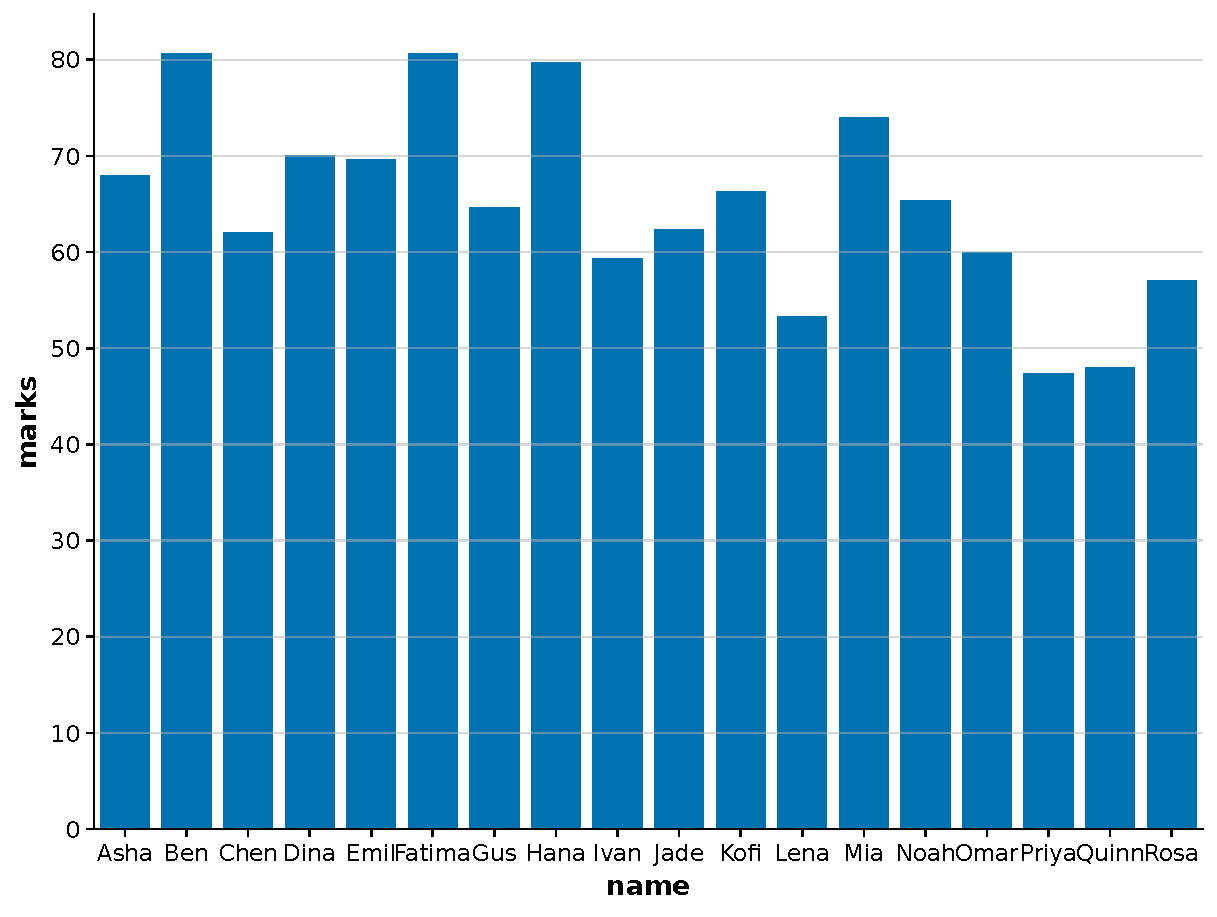
\includegraphics[width=0.72\textwidth,height=0.36\textheight,keepaspectratio]{figures/lesson01_example1_lesson1.pdf}
\captionof{figure}{Lesson 1, example: \code{lesson1.\allowbreak{}png}.}
\end{minipage}\end{center}
\begin{goodtoknow}
\begin{itemize}
  \item Each line is an instruction to the chart: \code{chart.\allowbreak{}draw\_\allowbreak{}bars}, \code{chart.\allowbreak{}draw\_\allowbreak{}lines}, \code{chart.\allowbreak{}draw\_\allowbreak{}dots} ... The chart is the thing, and \code{draw\_\allowbreak{}bars} says what it should do.
  \item For your own data, write chart = \code{sdata.\allowbreak{}chart(\textquotedbl{}my\_\allowbreak{}marks.\allowbreak{}xlsx\textquotedbl{})}. Excel, CSV, TSV, Parquet and JSON files all work.
  \item \code{chart.\allowbreak{}save(\textquotedbl{}lesson1.\allowbreak{}pdf\textquotedbl{})} saves a PDF instead: the end of the name decides the type.
  \item In Jupyter, VS Code or Spyder, write chart on the last line of a cell and the chart appears by itself. In a script, \code{chart.\allowbreak{}show()} opens it in a window.
  \item Are the names under the bars bumping into each other? Lesson 2 shows how to turn them.
  \item Learning on your own? \code{sdata.\allowbreak{}start\_\allowbreak{}30\_\allowbreak{}days()} turns the everyday lessons into 30 days of about an hour: each day starts with a few questions on earlier days and ends with a task. Then type \code{sdata.\allowbreak{}show\_\allowbreak{}today()} each day (or \code{sdata.\allowbreak{}start\_\allowbreak{}30\_\allowbreak{}days(track=\textquotedbl{}beginner\textquotedbl{})} if you have never programmed).
\end{itemize}
\end{goodtoknow}
\begin{tryit}
\begin{enumerate}
  \item Change \code{x=\textquotedbl{}name\textquotedbl{}} to \code{x=\textquotedbl{}subject\textquotedbl{}}. What does each bar show now?
  \item Save the chart as \code{\textquotedbl{}my\_\allowbreak{}first\_\allowbreak{}chart.\allowbreak{}png\textquotedbl{}} and also as \code{\textquotedbl{}my\_\allowbreak{}first\_\allowbreak{}chart.\allowbreak{}pdf\textquotedbl{}}.
  \item Make a chart of the \code{\textquotedbl{}fruit\textquotedbl{}} table: bars with \code{x=\textquotedbl{}fruit\textquotedbl{}} and \code{y=\textquotedbl{}count\textquotedbl{}}.
\end{enumerate}
Worked solutions: page~\pageref{solutions:1}, or type \code{sdata.\allowbreak{}show\_\allowbreak{}lesson(1,\allowbreak{} solutions=True)}.
\end{tryit}
\par\noindent{\small\sffamily\textbf{Words in this lesson:} \hyperref[word:sdata.get-example]{\code{sdata.\allowbreak{}get\_\allowbreak{}example()}}, \hyperref[word:sdata.chart]{\code{sdata.\allowbreak{}chart()}}, \hyperref[word:draw-bars]{\code{chart.\allowbreak{}draw\_\allowbreak{}bars()}}, \hyperref[word:save]{\code{chart.\allowbreak{}save()}}, \hyperref[word:show]{\code{chart.\allowbreak{}show()}}, \hyperref[word:sdata.start-30-days]{\code{sdata.\allowbreak{}start\_\allowbreak{}30\_\allowbreak{}days()}}, \hyperref[word:sdata.show-today]{\code{sdata.\allowbreak{}show\_\allowbreak{}today()}}.\par}

\chapter{Titles and labels}\label{lesson:2}
\begin{learnbox}
\begin{itemize}
  \item how to put a title on top
  \item how to name the x-axis and the y-axis
  \item how to add a small caption and change the size of the text
\end{itemize}
\end{learnbox}
\section*{Example 1}
A chart is easier to read when it says what it shows. First draw, then add the words.
\begin{lstlisting}[style=py]
import simplydata as sdata
marks = sdata.get_example("marks")
chart = sdata.chart(marks)
chart.draw_bars(x="name", y="marks")
chart.write_title_on_top("Our class marks")
chart.label_x("Student")
chart.label_y("Average mark")
chart.rotate_labels_x(45)
chart.write_caption_at_bottom("Made-up data from sdata.get_example")
chart.use_font_size(14)
chart.save("lesson2.png")
\end{lstlisting}
\whateachline
\begin{lineexplain}
  \item[1] Load simplydata.
  \item[2] Get the marks table.
  \item[3] Start a chart.
  \item[4] Draw one bar for each child.
  \item[5] Write a title on top of the chart.
  \item[6] Write a name under the x-axis (the bottom).
  \item[7] Write a name beside the y-axis (the side).
  \item[8] Turn the names under the bars by 45 degrees, so long names do not bump into each other.
  \item[9] Write a small line under the whole chart.
  \item[10] Make all the text a bit bigger (normal is 12).
  \item[11] Save it.
\end{lineexplain}
\printedoutput{output/lesson02_example1.txt}
\begin{center}\begin{minipage}{\linewidth}\centering
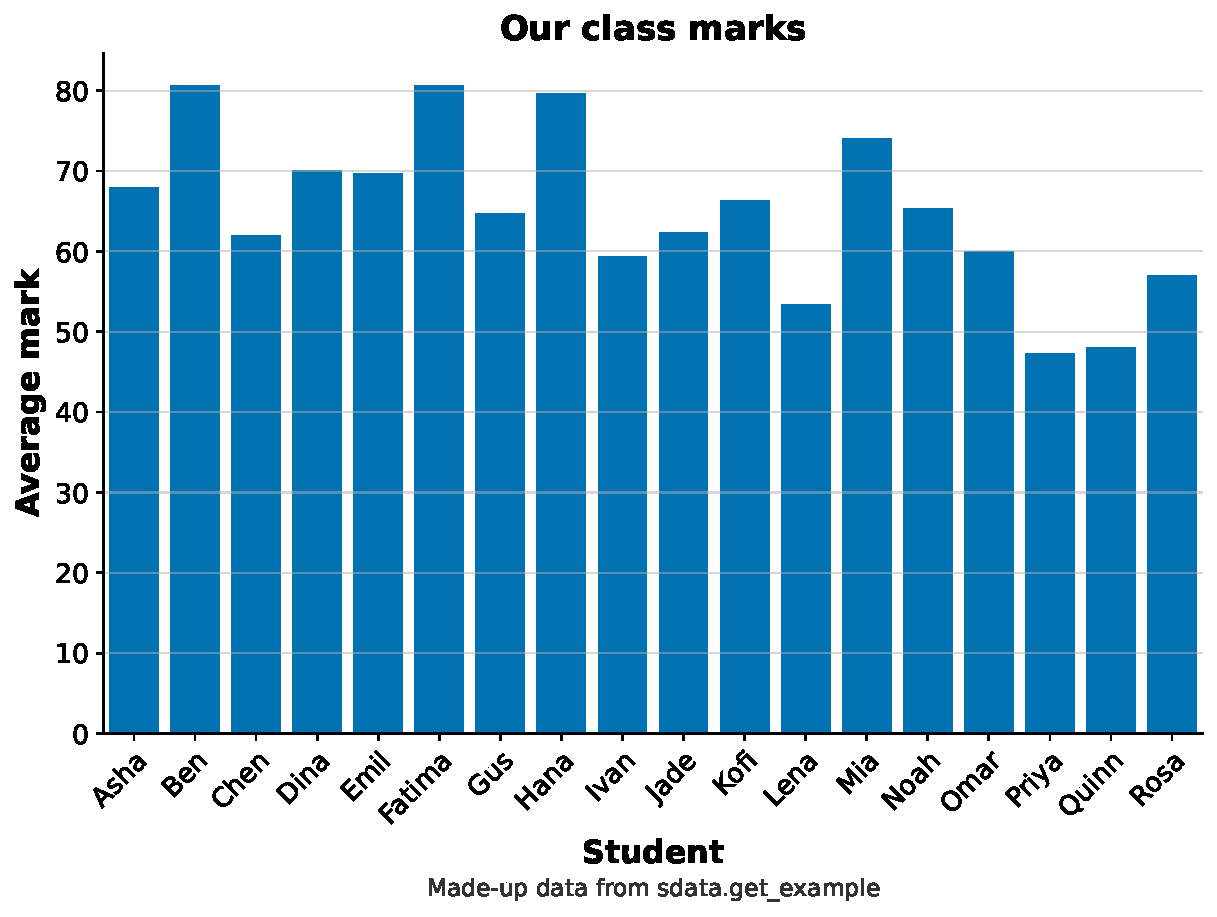
\includegraphics[width=0.72\textwidth,height=0.36\textheight,keepaspectratio]{figures/lesson02_example1_lesson2.pdf}
\captionof{figure}{Lesson 2, example 1: \code{lesson2.\allowbreak{}png}.}
\end{minipage}\end{center}
\section*{Example 2}
Words can also go next to the dots: a name for each dot, where it covers nothing.
\begin{lstlisting}[style=py]
import simplydata as sdata
kids = {"name": ["Asha", "Ben", "Chen", "Dina", "Eli"], "hours": [2.0, 5.5, 3.1, 7.2, 4.4], "marks": [48, 71, 55, 88, 62]}
chart = sdata.chart(kids)
chart.draw_dots(x="hours", y="marks")
chart.write_names_on_dots("name")
chart.label_x("Hours of study")
chart.save("lesson2_names.png")
\end{lstlisting}
\whateachline
\begin{lineexplain}
  \item[1] Load simplydata.
  \item[2] A small table typed by hand: each column name, then its values in a list.
  \item[3] Start a chart of it.
  \item[4] One dot for each child.
  \item[5] Write each name next to its dot, where it covers no other name or dot. A name with no free place is left out, and a line says so.
  \item[6] Name the x-axis.
  \item[7] Save it.
\end{lineexplain}
\printedoutput{output/lesson02_example2.txt}
\begin{center}\begin{minipage}{\linewidth}\centering
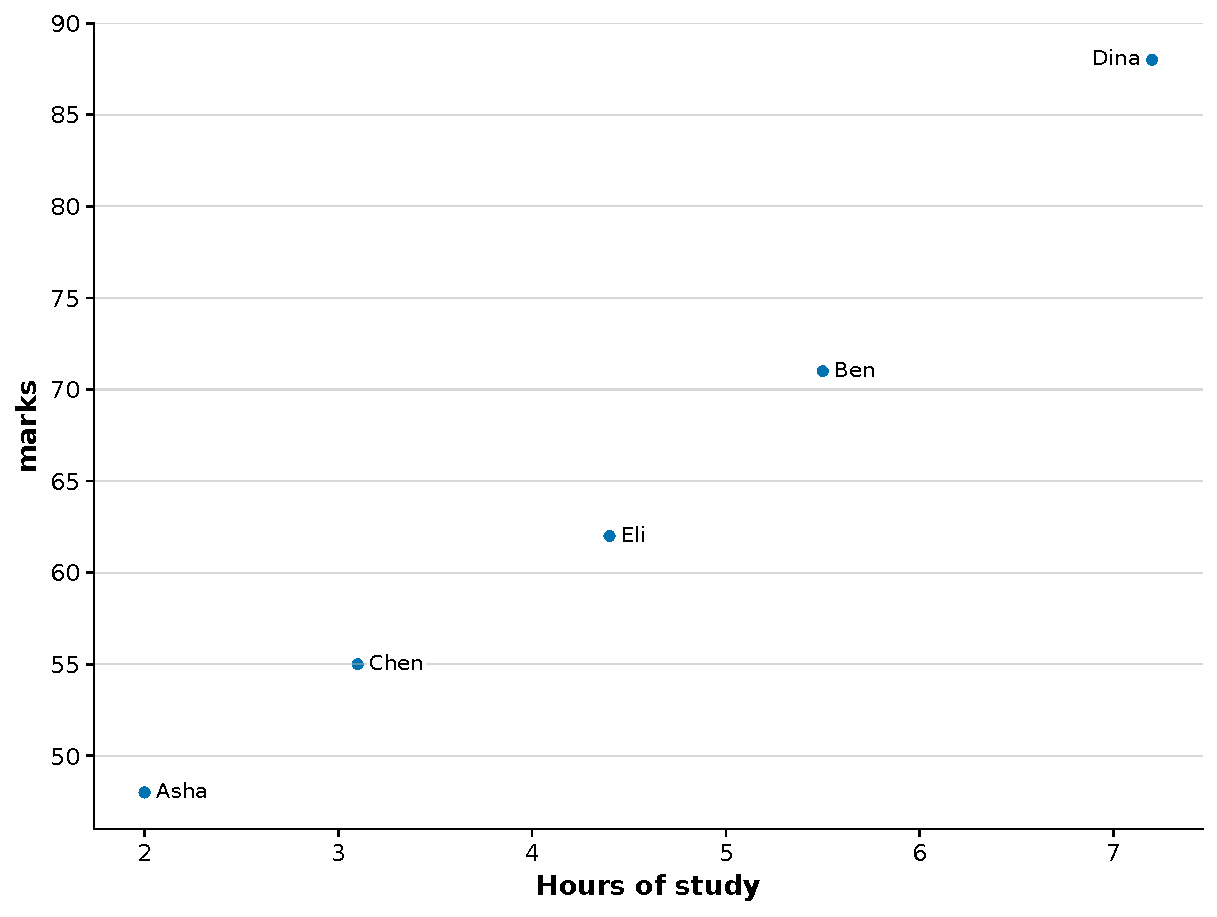
\includegraphics[width=0.72\textwidth,height=0.36\textheight,keepaspectratio]{figures/lesson02_example2_lesson2_names.pdf}
\captionof{figure}{Lesson 2, example 2: \code{lesson2\_\allowbreak{}names.\allowbreak{}png}.}
\end{minipage}\end{center}
\begin{goodtoknow}
\begin{itemize}
  \item After the chart type, the order of words such as \code{write\_\allowbreak{}title\_\allowbreak{}on\_\allowbreak{}top} and \code{label\_\allowbreak{}y} does not matter: the chart is drawn when you save or show it.
  \item Words that belong to one axis end in \_x or \_y: \code{label\_\allowbreak{}x}, \code{label\_\allowbreak{}y}, \code{rotate\_\allowbreak{}labels\_\allowbreak{}x}.
\end{itemize}
\end{goodtoknow}
\begin{tryit}
\begin{enumerate}
  \item Give the chart your own title, and label the y-axis \code{\textquotedbl{}Marks out of 100\textquotedbl{}}.
  \item Try \code{chart.\allowbreak{}use\_\allowbreak{}font\_\allowbreak{}size(20)}. Then try 9. Which is easier to read?
  \item Take away the line \code{chart.\allowbreak{}rotate\_\allowbreak{}labels\_\allowbreak{}x(45)}. What happens to the names?
\end{enumerate}
Worked solutions: page~\pageref{solutions:2}, or type \code{sdata.\allowbreak{}show\_\allowbreak{}lesson(2,\allowbreak{} solutions=True)}.
\end{tryit}
\par\noindent{\small\sffamily\textbf{Words in this lesson:} \hyperref[word:write-title-on-top]{\code{chart.\allowbreak{}write\_\allowbreak{}title\_\allowbreak{}on\_\allowbreak{}top()}}, \hyperref[word:label-x]{\code{chart.\allowbreak{}label\_\allowbreak{}x()}}, \hyperref[word:label-y]{\code{chart.\allowbreak{}label\_\allowbreak{}y()}}, \hyperref[word:rotate-labels-x]{\code{chart.\allowbreak{}rotate\_\allowbreak{}labels\_\allowbreak{}x()}}, \hyperref[word:write-caption-at-bottom]{\code{chart.\allowbreak{}write\_\allowbreak{}caption\_\allowbreak{}at\_\allowbreak{}bottom()}}, \hyperref[word:use-font-size]{\code{chart.\allowbreak{}use\_\allowbreak{}font\_\allowbreak{}size()}}, \hyperref[word:write-names-on-dots]{\code{chart.\allowbreak{}write\_\allowbreak{}names\_\allowbreak{}on\_\allowbreak{}dots()}}.\par}

\chapter{Colours, groups and legends}\label{lesson:3}
\begin{learnbox}
\begin{itemize}
  \item how to give each group its own colour
  \item how to choose your own colours
  \item how to move the legend (the box that says which colour is which)
  \item how to change the whole look with a style
\end{itemize}
\end{learnbox}
\section*{Example 1}
\code{colour=} inside a chart type splits the data into groups.
\begin{lstlisting}[style=py]
import simplydata as sdata
marks = sdata.get_example("marks")
chart = sdata.chart(marks)
chart.draw_bars(x="subject", y="marks", colour="class")
chart.use_colours("orange", "teal", "purple")
chart.put_legend_at_bottom()
chart.write_title_on_top("Marks in each subject")
chart.save("lesson3_groups.png")
\end{lstlisting}
\whateachline
\begin{lineexplain}
  \item[1] Load simplydata.
  \item[2] Get the marks table.
  \item[3] Start a chart.
  \item[4] For each subject, draw one bar per class, each class in its own colour.
  \item[5] Choose the colours yourself, in order: class A orange, B teal, C purple.
  \item[6] Put the legend under the chart.
  \item[7] Add a title.
  \item[8] Save it.
\end{lineexplain}
\printedoutput{output/lesson03_example1.txt}
\begin{center}\begin{minipage}{\linewidth}\centering
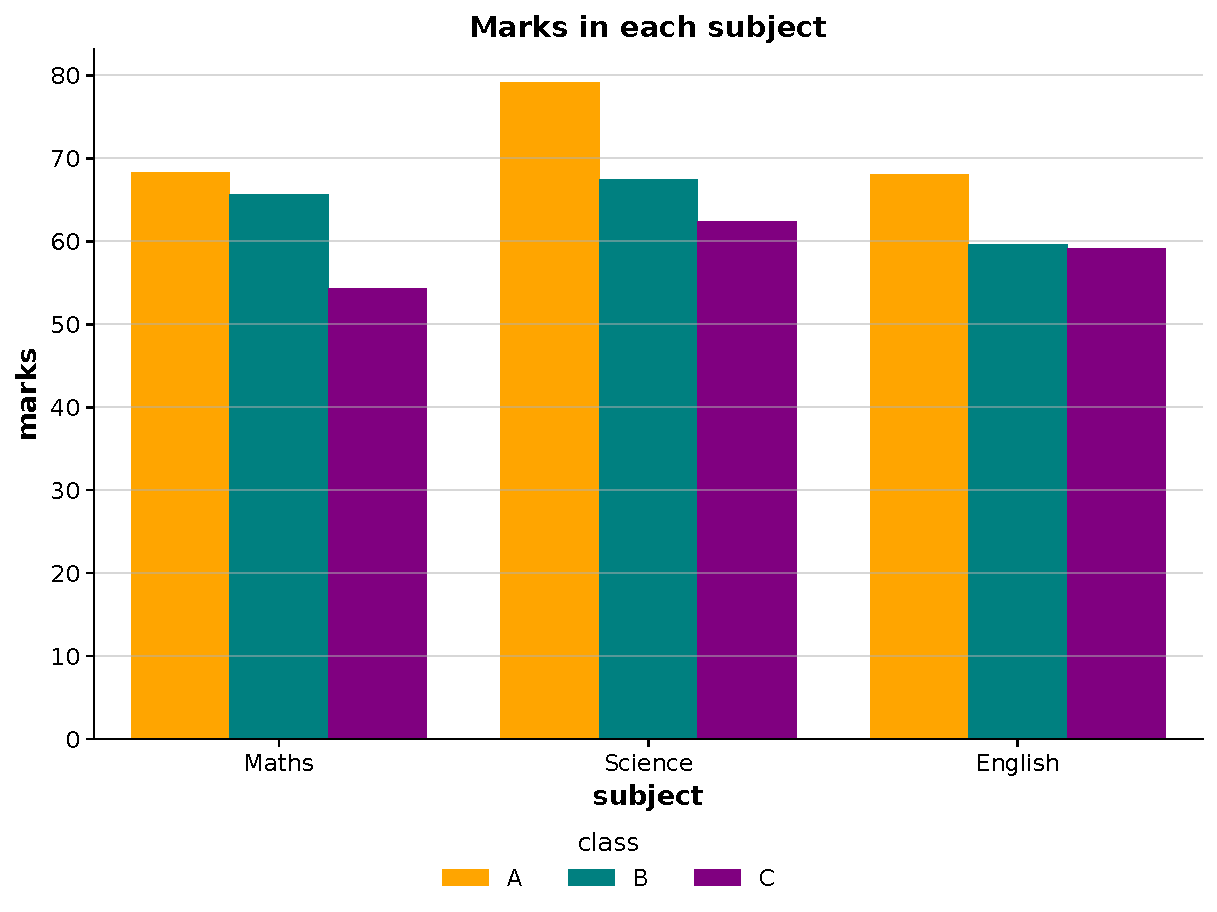
\includegraphics[width=0.72\textwidth,height=0.36\textheight,keepaspectratio]{figures/lesson03_example1_lesson3_groups.pdf}
\captionof{figure}{Lesson 3, example 1: \code{lesson3\_\allowbreak{}groups.\allowbreak{}png}.}
\end{minipage}\end{center}
\section*{Example 2}
Without groups, one colour is used for everything. You can choose it.
\begin{lstlisting}[style=py]
import simplydata as sdata
weather = sdata.get_example("weather")
chart = sdata.chart(weather)
chart.draw_lines(x="month", y="rain")
chart.use_colour("blue")
chart.use_style("school")
chart.save("lesson3_look.png")
\end{lstlisting}
\whateachline
\begin{lineexplain}
  \item[1] Load simplydata.
  \item[2] Get the weather table: three made-up cities.
  \item[3] Start a chart.
  \item[4] Draw a line of rain through the months. With three cities in each month, the line shows their average.
  \item[5] Make the line blue.
  \item[6] Change the whole look. Try \code{\textquotedbl{}paper\textquotedbl{}}, \code{\textquotedbl{}school\textquotedbl{}}, \code{\textquotedbl{}presentation\textquotedbl{}} and \code{\textquotedbl{}dark\textquotedbl{}}.
  \item[7] Save it.
\end{lineexplain}
\printedoutput{output/lesson03_example2.txt}
\begin{center}\begin{minipage}{\linewidth}\centering
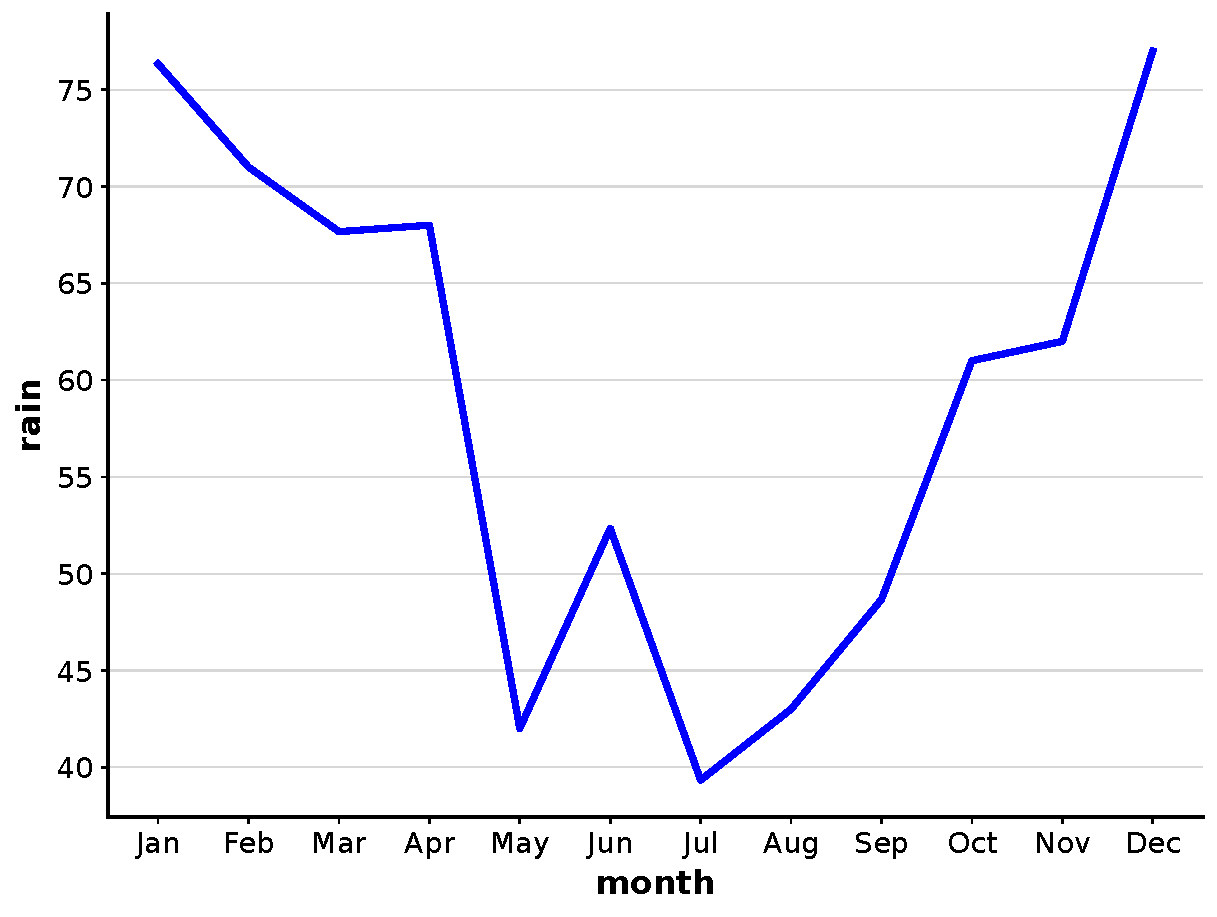
\includegraphics[width=0.72\textwidth,height=0.36\textheight,keepaspectratio]{figures/lesson03_example2_lesson3_look.pdf}
\captionof{figure}{Lesson 3, example 2: \code{lesson3\_\allowbreak{}look.\allowbreak{}png}.}
\end{minipage}\end{center}
\section*{Example 3}
Groups come in the order they first appear in the table. You can choose another order, and give the legend a name.
\begin{lstlisting}[style=py]
import simplydata as sdata
marks = sdata.get_example("marks")
chart = sdata.chart(marks)
chart.draw_bars(x="class", y="marks", colour="subject")
chart.order_x("C", "B", "A")
chart.order_legend("Science", "Maths", "English")
chart.label_legend("Subject")
chart.save("lesson3_order.png")
\end{lstlisting}
\whateachline
\begin{lineexplain}
  \item[1] Load simplydata.
  \item[2] Get the marks table.
  \item[3] Start a chart.
  \item[4] For each class, one bar per subject.
  \item[5] Put the classes along the x-axis in this order.
  \item[6] Put the subjects in this order: in the legend and side by side in each class.
  \item[7] The name above the legend (normally the column name).
  \item[8] Save it.
\end{lineexplain}
\printedoutput{output/lesson03_example3.txt}
\begin{center}\begin{minipage}{\linewidth}\centering
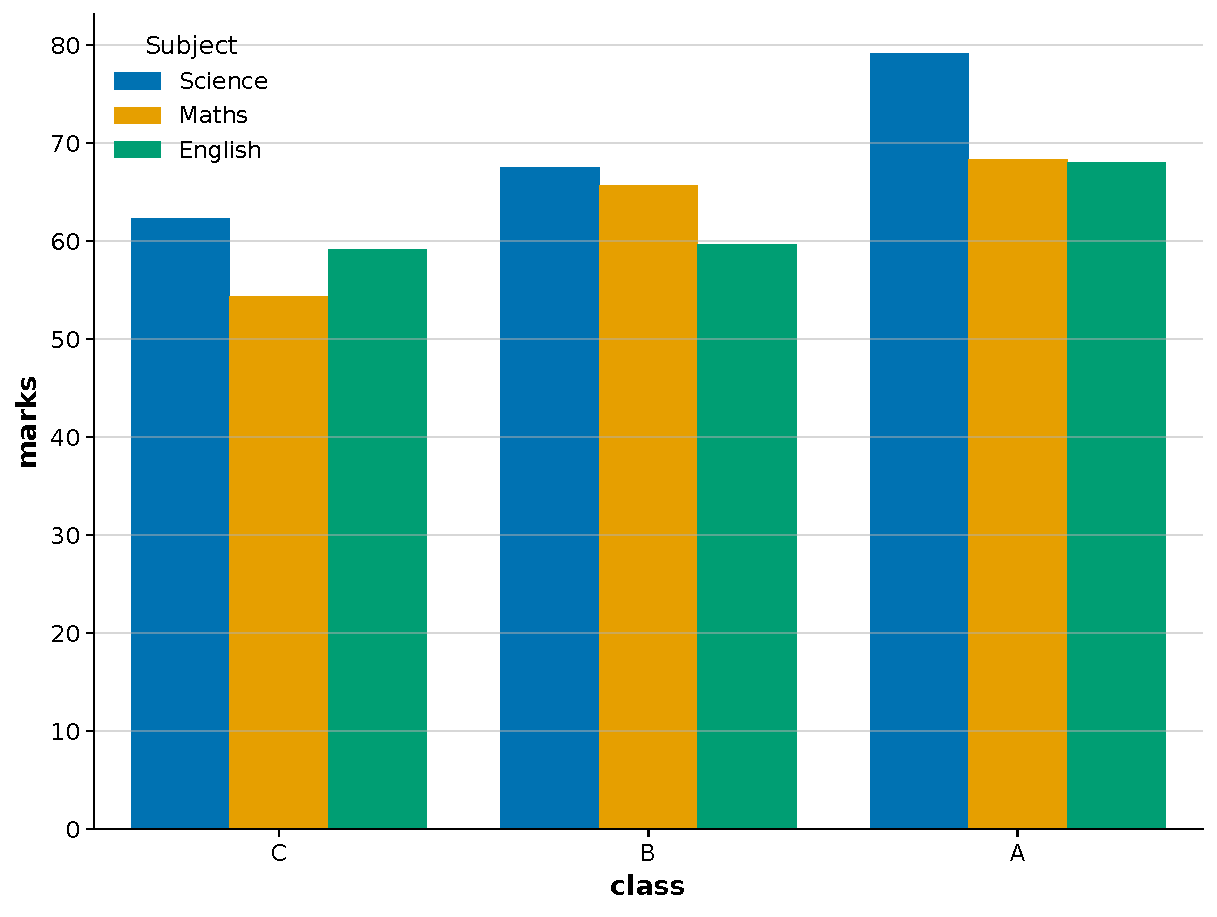
\includegraphics[width=0.72\textwidth,height=0.36\textheight,keepaspectratio]{figures/lesson03_example3_lesson3_order.pdf}
\captionof{figure}{Lesson 3, example 3: \code{lesson3\_\allowbreak{}order.\allowbreak{}png}.}
\end{minipage}\end{center}
\section*{Example 4}
Numbers can have colours too: a colour scale. And dots that overlap are easier to see when they let the others show through.
\begin{lstlisting}[style=py]
import simplydata as sdata
weather = sdata.get_example("weather")
chart = sdata.chart(weather)
chart.draw_heatmap(x="month", y="city", value="temperature")
chart.use_colour_scale("blue to red", middle=10)
chart.save("lesson3_colour_scale.png")
marks = sdata.get_example("marks")
dots = sdata.chart(marks)
dots.draw_dots(x="hours", y="marks", colour="class", transparency=0.5)
dots.save("lesson3_transparency.png")
\end{lstlisting}
\whateachline
\begin{lineexplain}
  \item[1] Load simplydata.
  \item[2] Get the weather table.
  \item[3] Start a chart.
  \item[4] One square per city and month, coloured by temperature.
  \item[5] Blue below 10 \textdegree{}C, red above, white at 10. \code{middle=} makes a scale that goes two ways.
  \item[6] Save it.
  \item[7] Get the marks table.
  \item[8] A second chart.
  \item[9] \code{transparency=0.\allowbreak{}5} makes each dot half see-through, so dots on top of each other show.
  \item[10] Save it.
\end{lineexplain}
\printedoutput{output/lesson03_example4.txt}
\begin{center}\begin{minipage}{\linewidth}\centering
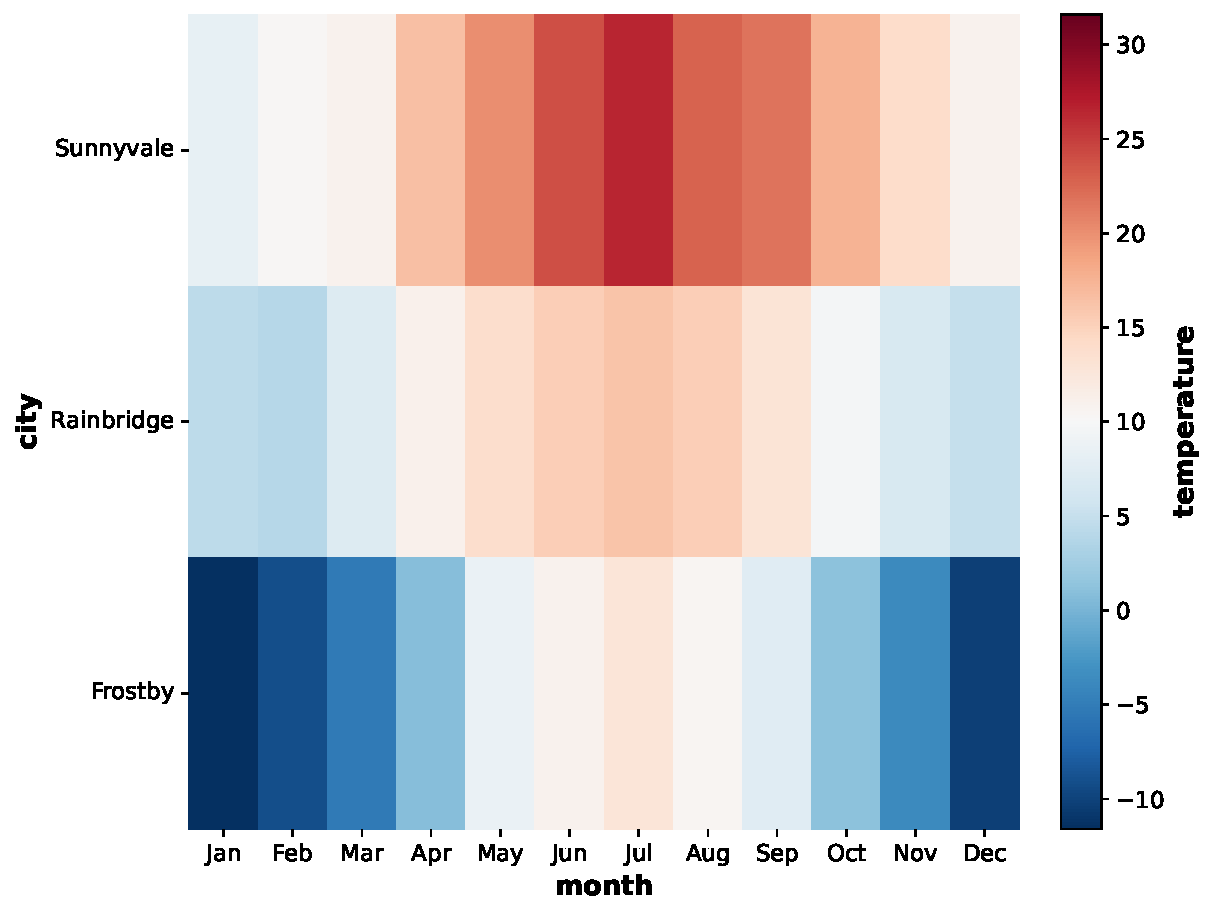
\includegraphics[width=0.48\textwidth,height=0.36\textheight,keepaspectratio]{figures/lesson03_example4_lesson3_colour_scale.pdf}\hfill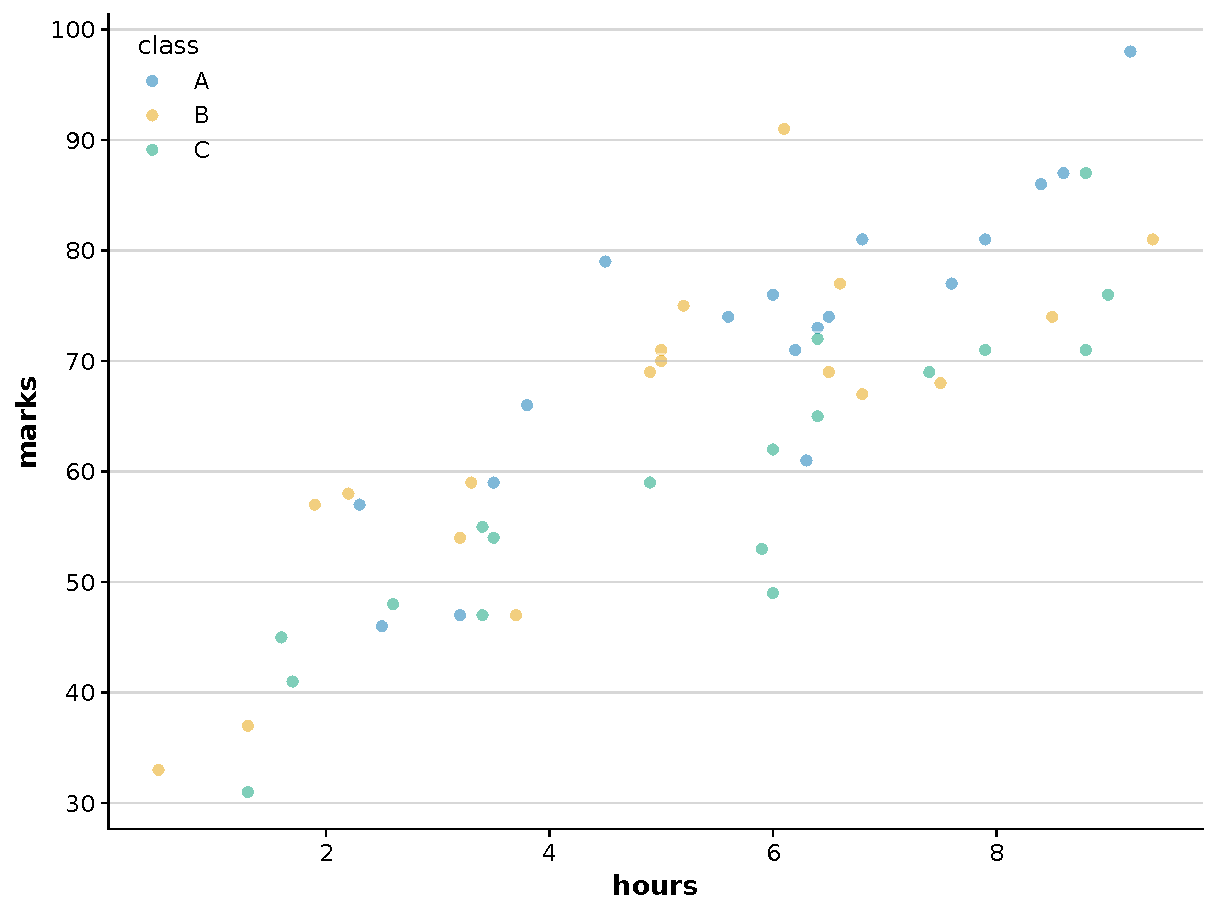
\includegraphics[width=0.48\textwidth,height=0.36\textheight,keepaspectratio]{figures/lesson03_example4_lesson3_transparency.pdf}
\captionof{figure}{Lesson 3, example 4: \code{lesson3\_\allowbreak{}colour\_\allowbreak{}scale.\allowbreak{}png} and \code{lesson3\_\allowbreak{}transparency.\allowbreak{}png}.}
\end{minipage}\end{center}
\begin{goodtoknow}
\begin{itemize}
  \item \code{colour=\textquotedbl{}class\textquotedbl{}} (a column) gives each group a colour. \code{colour=\textquotedbl{}red\textquotedbl{}} (a colour) makes that step red. color works too.
  \item The legend can go on any side: \code{put\_\allowbreak{}legend\_\allowbreak{}at\_\allowbreak{}top}, \code{put\_\allowbreak{}legend\_\allowbreak{}at\_\allowbreak{}bottom}, \code{put\_\allowbreak{}legend\_\allowbreak{}on\_\allowbreak{}left}, \code{put\_\allowbreak{}legend\_\allowbreak{}on\_\allowbreak{}right}. \code{hide\_\allowbreak{}legend} takes it away and \code{show\_\allowbreak{}legend} brings it back.
  \item Month and weekday names (\code{\textquotedbl{}Jan\textquotedbl{}}, \code{\textquotedbl{}Monday\textquotedbl{}}) come in calendar order by themselves, also in the small charts of \code{draw\_\allowbreak{}one\_\allowbreak{}chart\_\allowbreak{}for\_\allowbreak{}each\_\allowbreak{}group\_\allowbreak{}in} and the frames of animate. \code{order\_\allowbreak{}x(biggest\_\allowbreak{}first=True)} puts the biggest bar first, and \code{order\_\allowbreak{}y} orders the groups up the y-axis.
\end{itemize}
\end{goodtoknow}
\begin{tryit}
\begin{enumerate}
  \item In the weather chart, add \code{colour=\textquotedbl{}city\textquotedbl{}} to \code{chart.\allowbreak{}draw\_\allowbreak{}lines(.\allowbreak{}.\allowbreak{}.\allowbreak{})}. How many lines do you get?
  \item Move the legend to the top with \code{chart.\allowbreak{}put\_\allowbreak{}legend\_\allowbreak{}at\_\allowbreak{}top()}.
  \item Try \code{chart.\allowbreak{}use\_\allowbreak{}style(\textquotedbl{}dark\textquotedbl{})} and choose three colours that look good on it.
\end{enumerate}
Worked solutions: page~\pageref{solutions:3}, or type \code{sdata.\allowbreak{}show\_\allowbreak{}lesson(3,\allowbreak{} solutions=True)}.
\end{tryit}
\par\noindent{\small\sffamily\textbf{Words in this lesson:} \hyperref[word:use-colours]{\code{chart.\allowbreak{}use\_\allowbreak{}colours()}}, \hyperref[word:use-colour]{\code{chart.\allowbreak{}use\_\allowbreak{}colour()}}, \hyperref[word:use-colour-scale]{\code{chart.\allowbreak{}use\_\allowbreak{}colour\_\allowbreak{}scale()}}, \hyperref[word:put-legend-at-bottom]{\code{chart.\allowbreak{}put\_\allowbreak{}legend\_\allowbreak{}at\_\allowbreak{}bottom()}}, \hyperref[word:put-legend-at-top]{\code{chart.\allowbreak{}put\_\allowbreak{}legend\_\allowbreak{}at\_\allowbreak{}top()}}, \hyperref[word:hide-legend]{\code{chart.\allowbreak{}hide\_\allowbreak{}legend()}}, \hyperref[word:use-style]{\code{chart.\allowbreak{}use\_\allowbreak{}style()}}, \hyperref[word:draw-lines]{\code{chart.\allowbreak{}draw\_\allowbreak{}lines()}}, \hyperref[word:order-x]{\code{chart.\allowbreak{}order\_\allowbreak{}x()}}, \hyperref[word:order-legend]{\code{chart.\allowbreak{}order\_\allowbreak{}legend()}}, \hyperref[word:label-legend]{\code{chart.\allowbreak{}label\_\allowbreak{}legend()}}.\par}

\chapter{Different chart types}\label{lesson:4}
\begin{learnbox}
\begin{itemize}
  \item lines, dots, histograms, boxes and pies
  \item which chart suits which question
  \item how to put two chart types on top of each other
\end{itemize}
\end{learnbox}
\section*{Example 1}
Lines show how something changes, for example over time.
\begin{lstlisting}[style=py]
import simplydata as sdata
weather = sdata.get_example("weather")
chart = sdata.chart(weather)
chart.draw_lines(x="month", y="temperature", colour="city", with_dots=True)
chart.save("lesson4_lines.png")
\end{lstlisting}
\whateachline
\begin{lineexplain}
  \item[1] Load simplydata.
  \item[2] Get the weather table.
  \item[3] Start a chart.
  \item[4] One line per city. \code{with\_\allowbreak{}dots=True} also marks each month with a dot.
  \item[5] Save it.
\end{lineexplain}
\printedoutput{output/lesson04_example1.txt}
\begin{center}\begin{minipage}{\linewidth}\centering
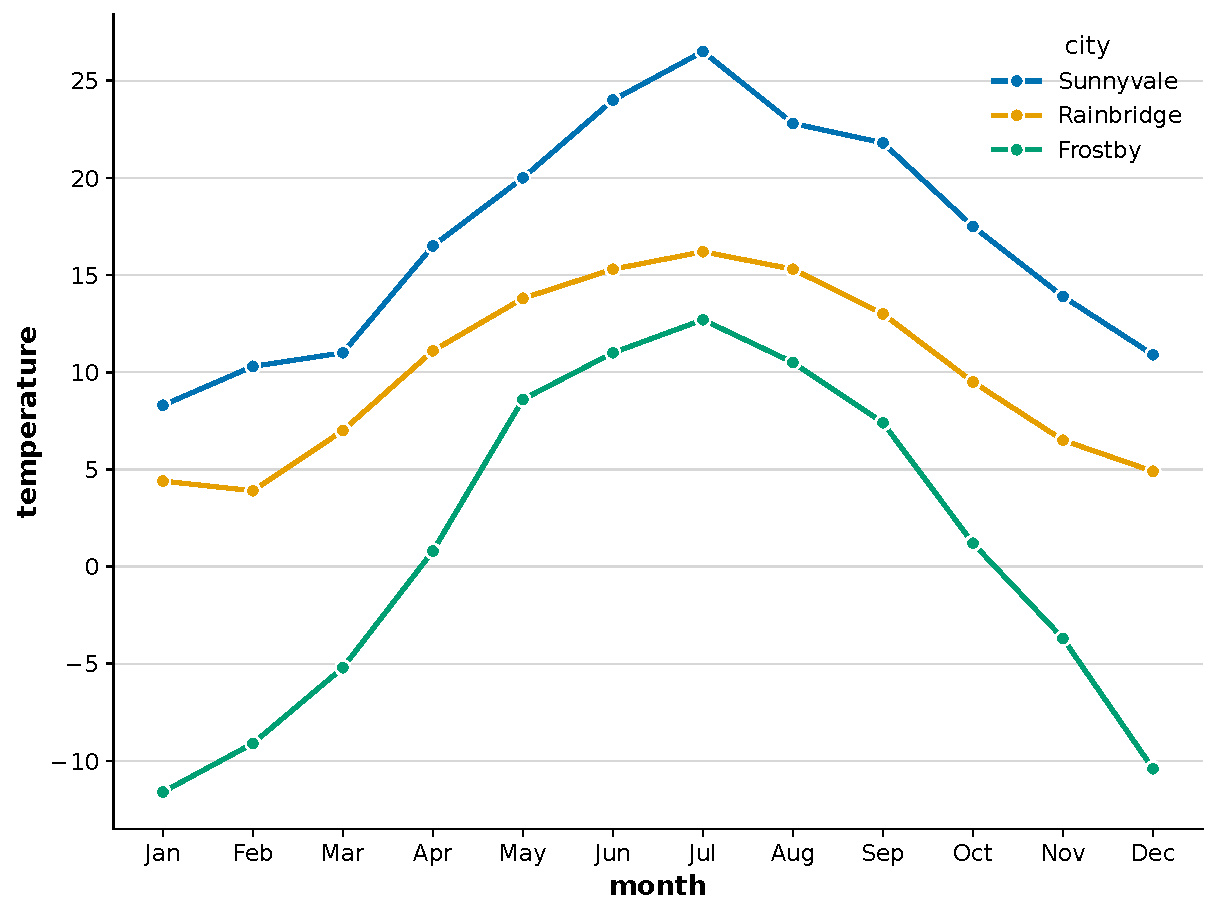
\includegraphics[width=0.72\textwidth,height=0.36\textheight,keepaspectratio]{figures/lesson04_example1_lesson4_lines.pdf}
\captionof{figure}{Lesson 4, example 1: \code{lesson4\_\allowbreak{}lines.\allowbreak{}png}.}
\end{minipage}\end{center}
\section*{Example 2}
Dots show if two things go together. This is also called a scatter chart.
\begin{lstlisting}[style=py]
import simplydata as sdata
marks = sdata.get_example("marks")
chart = sdata.chart(marks)
chart.draw_dots(x="hours", y="marks", colour="class")
chart.save("lesson4_dots.png")
\end{lstlisting}
\whateachline
\begin{lineexplain}
  \item[1] Load simplydata.
  \item[2] Get the marks table.
  \item[3] Start a chart.
  \item[4] One dot for each test: how long the child studied, and the mark they got.
  \item[5] Save it. Do more hours give more marks?
\end{lineexplain}
\printedoutput{output/lesson04_example2.txt}
\begin{center}\begin{minipage}{\linewidth}\centering
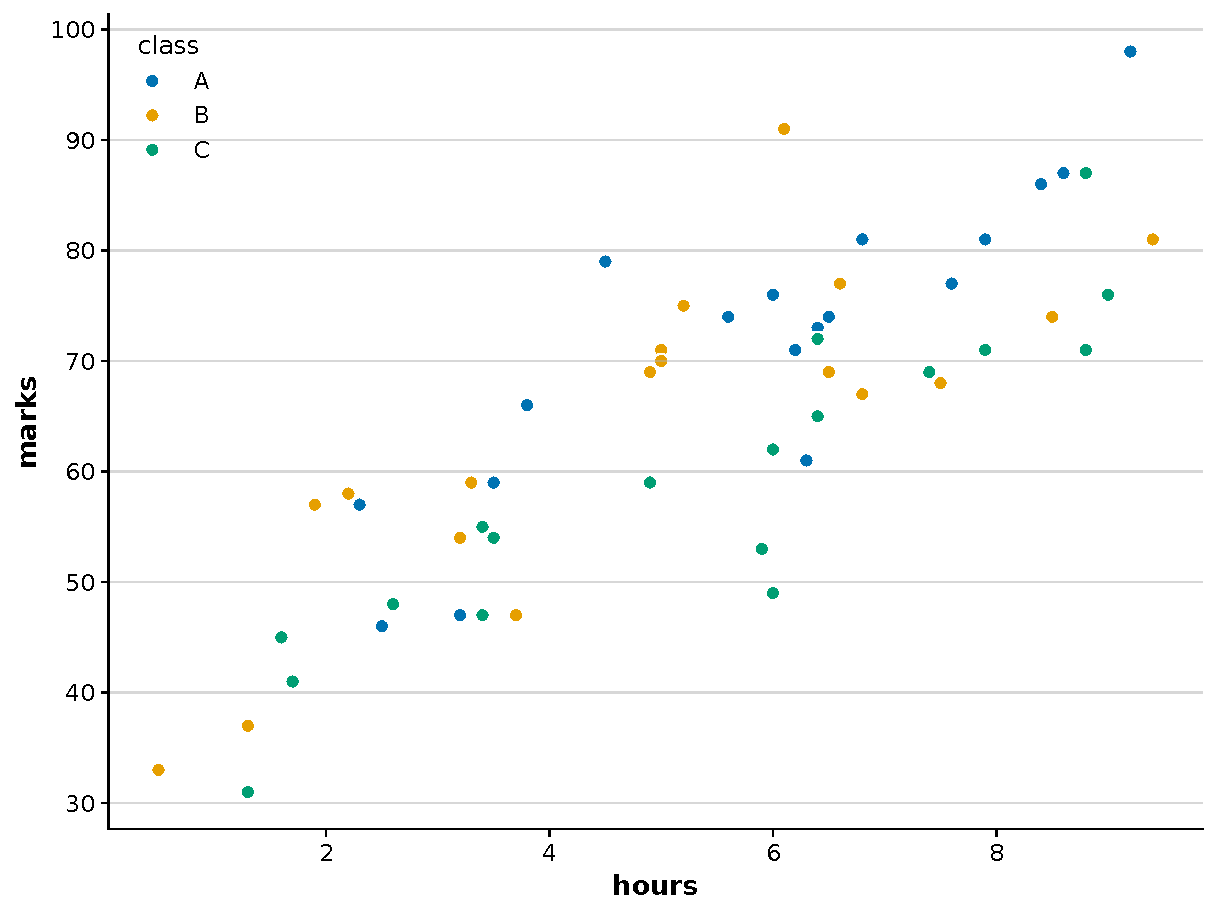
\includegraphics[width=0.72\textwidth,height=0.36\textheight,keepaspectratio]{figures/lesson04_example2_lesson4_dots.pdf}
\captionof{figure}{Lesson 4, example 2: \code{lesson4\_\allowbreak{}dots.\allowbreak{}png}.}
\end{minipage}\end{center}
\section*{Example 3}
A histogram counts how many values fall in each range, like 40 to 50, 50 to 60 ... Its shape is called the distribution of the values.
\begin{lstlisting}[style=py]
import simplydata as sdata
marks = sdata.get_example("marks")
chart = sdata.chart(marks)
chart.draw_histogram(x="marks", with_bins=8)
chart.save("lesson4_histogram.png")
\end{lstlisting}
\whateachline
\begin{lineexplain}
  \item[1] Load simplydata.
  \item[2] Get the marks table.
  \item[3] Start a chart.
  \item[4] Cut the marks into 8 ranges (bins) and draw a bar for how many marks are in each.
  \item[5] Save it.
\end{lineexplain}
\printedoutput{output/lesson04_example3.txt}
\begin{center}\begin{minipage}{\linewidth}\centering
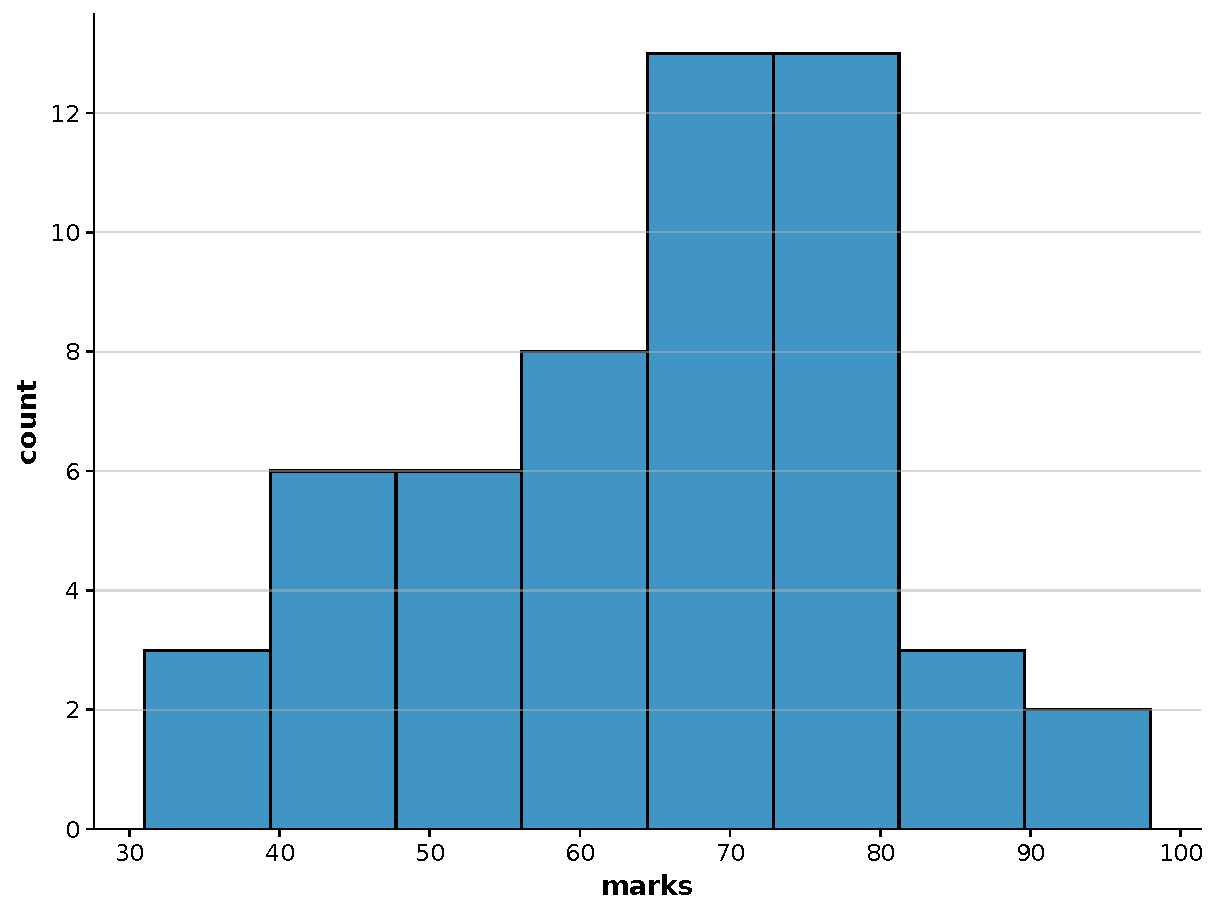
\includegraphics[width=0.72\textwidth,height=0.36\textheight,keepaspectratio]{figures/lesson04_example3_lesson4_histogram.pdf}
\captionof{figure}{Lesson 4, example 3: \code{lesson4\_\allowbreak{}histogram.\allowbreak{}png}.}
\end{minipage}\end{center}
\section*{Example 4}
Boxes show how spread out the values are. Two chart types on one chart are drawn one on top of the other.
\begin{lstlisting}[style=py]
import simplydata as sdata
marks = sdata.get_example("marks")
chart = sdata.chart(marks)
chart.draw_boxes(x="class", y="marks")
chart.draw_all_dots(x="class", y="marks")
chart.save("lesson4_boxes.png")
\end{lstlisting}
\whateachline
\begin{lineexplain}
  \item[1] Load simplydata.
  \item[2] Get the marks table.
  \item[3] Start a chart.
  \item[4] One box per class. The line in the box is the median: the middle mark when they are put in order. The box holds the middle half of the marks (the interquartile range).
  \item[5] Also show every single mark as a dot, on top of the boxes.
  \item[6] Save it.
\end{lineexplain}
\printedoutput{output/lesson04_example4.txt}
\begin{center}\begin{minipage}{\linewidth}\centering
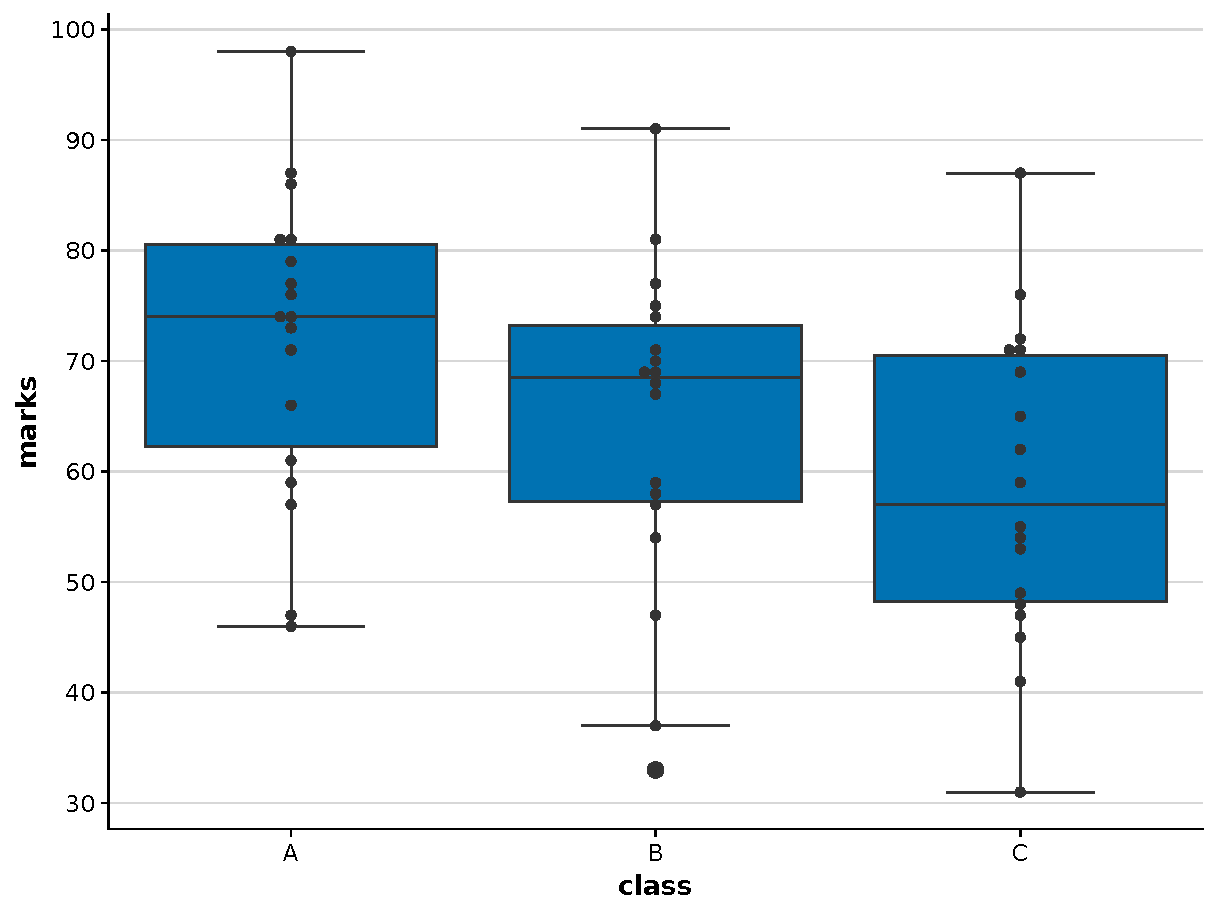
\includegraphics[width=0.72\textwidth,height=0.36\textheight,keepaspectratio]{figures/lesson04_example4_lesson4_boxes.pdf}
\captionof{figure}{Lesson 4, example 4: \code{lesson4\_\allowbreak{}boxes.\allowbreak{}png}.}
\end{minipage}\end{center}
\section*{Example 5}
A pie shows how a whole is shared out.
\begin{lstlisting}[style=py]
import simplydata as sdata
fruit = sdata.get_example("fruit")
chart = sdata.chart(fruit)
chart.draw_pie(labels="fruit", values="count")
chart.save("lesson4_pie.png")
\end{lstlisting}
\whateachline
\begin{lineexplain}
  \item[1] Load simplydata.
  \item[2] Get the fruit table: what two shops sold in a week.
  \item[3] Start a chart.
  \item[4] One slice per fruit, as big as the number sold.
  \item[5] Save it.
\end{lineexplain}
\printedoutput{output/lesson04_example5.txt}
\begin{center}\begin{minipage}{\linewidth}\centering
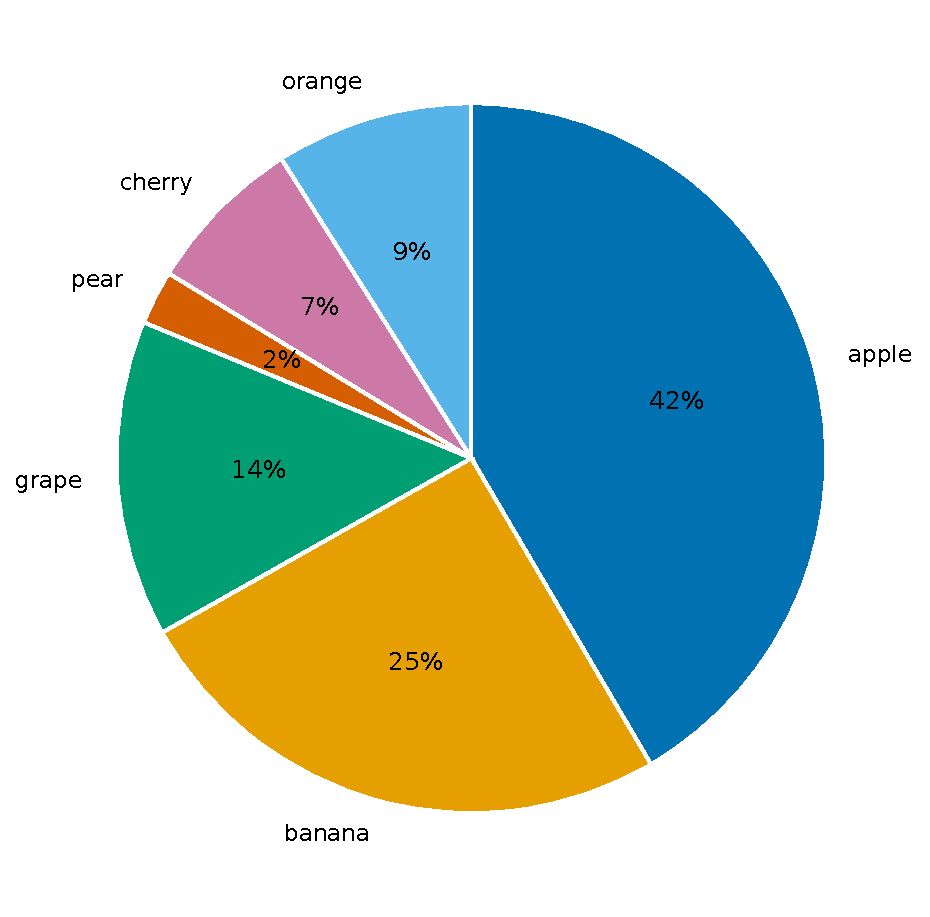
\includegraphics[width=0.72\textwidth,height=0.36\textheight,keepaspectratio]{figures/lesson04_example5_lesson4_pie.pdf}
\captionof{figure}{Lesson 4, example 5: \code{lesson4\_\allowbreak{}pie.\allowbreak{}png}.}
\end{minipage}\end{center}
\begin{goodtoknow}
\begin{itemize}
  \item Chart types on the same chart are layers of one chart. Lesson 7 shows how to make several charts and put them on one page.
  \item There are more chart types: \code{draw\_\allowbreak{}area}, \code{draw\_\allowbreak{}violins}, \code{draw\_\allowbreak{}heatmap}, \code{draw\_\allowbreak{}polar}, \code{draw\_\allowbreak{}contour}, \code{draw\_\allowbreak{}surface} and \code{draw\_\allowbreak{}dots\_\allowbreak{}3d}. Type \code{sdata.\allowbreak{}show\_\allowbreak{}all\_\allowbreak{}words()} to see them all and \code{sdata.\allowbreak{}help(\textquotedbl{}draw\_\allowbreak{}violins\textquotedbl{})} to learn one.
\end{itemize}
\end{goodtoknow}
\begin{tryit}
\begin{enumerate}
  \item Draw \code{chart.\allowbreak{}draw\_\allowbreak{}violins(x=\textquotedbl{}class\textquotedbl{},\allowbreak{} y=\textquotedbl{}marks\textquotedbl{})} instead of boxes. What is different?
  \item Draw a histogram of the weather \code{\textquotedbl{}temperature\textquotedbl{}} column with \code{with\_\allowbreak{}bins=6}.
  \item Make a chart of \code{sdata.\allowbreak{}get\_\allowbreak{}example(\textquotedbl{}growth\textquotedbl{})} and draw \code{chart.\allowbreak{}draw\_\allowbreak{}area(x=\textquotedbl{}year\textquotedbl{},\allowbreak{} y=\textquotedbl{}population\textquotedbl{},\allowbreak{} colour=\textquotedbl{}country\textquotedbl{})}.
\end{enumerate}
Worked solutions: page~\pageref{solutions:4}, or type \code{sdata.\allowbreak{}show\_\allowbreak{}lesson(4,\allowbreak{} solutions=True)}.
\end{tryit}
\par\noindent{\small\sffamily\textbf{Words in this lesson:} \hyperref[word:draw-lines]{\code{chart.\allowbreak{}draw\_\allowbreak{}lines()}}, \hyperref[word:draw-dots]{\code{chart.\allowbreak{}draw\_\allowbreak{}dots()}}, \hyperref[word:draw-histogram]{\code{chart.\allowbreak{}draw\_\allowbreak{}histogram()}}, \hyperref[word:draw-boxes]{\code{chart.\allowbreak{}draw\_\allowbreak{}boxes()}}, \hyperref[word:draw-all-dots]{\code{chart.\allowbreak{}draw\_\allowbreak{}all\_\allowbreak{}dots()}}, \hyperref[word:draw-pie]{\code{chart.\allowbreak{}draw\_\allowbreak{}pie()}}, \hyperref[word:draw-violins]{\code{chart.\allowbreak{}draw\_\allowbreak{}violins()}}, \hyperref[word:draw-area]{\code{chart.\allowbreak{}draw\_\allowbreak{}area()}}.\par}

\chapter{Statistics: averages, error bars and fit lines}\label{lesson:5}
\begin{learnbox}
\begin{itemize}
  \item what a bar shows when a group has many values: the average or the median
  \item how to add error bars, and the difference between standard deviation and standard error
  \item how to draw the straight line that fits some dots best
\end{itemize}
\end{learnbox}
\section*{Example 1}
The average (also called the mean) is all the values added up, divided by how many there are. Error bars show how far the values spread around it.
\begin{lstlisting}[style=py]
import simplydata as sdata
marks = sdata.get_example("marks")
chart = sdata.chart(marks)
chart.draw_bars(x="class", y="marks", show="average", error="standard deviation")
chart.write_numbers_on_bars()
chart.save("lesson5_average.png")
\end{lstlisting}
\whateachline
\begin{lineexplain}
  \item[1] Load simplydata.
  \item[2] Get the marks table.
  \item[3] Start a chart.
  \item[4] One bar per class, as tall as the average mark. The error bars show the standard deviation: how far marks usually are from the average. A line is printed that says which error bars were drawn.
  \item[5] Write the average on each bar.
  \item[6] Save it.
\end{lineexplain}
\printedoutput{output/lesson05_example1.txt}
\begin{center}\begin{minipage}{\linewidth}\centering
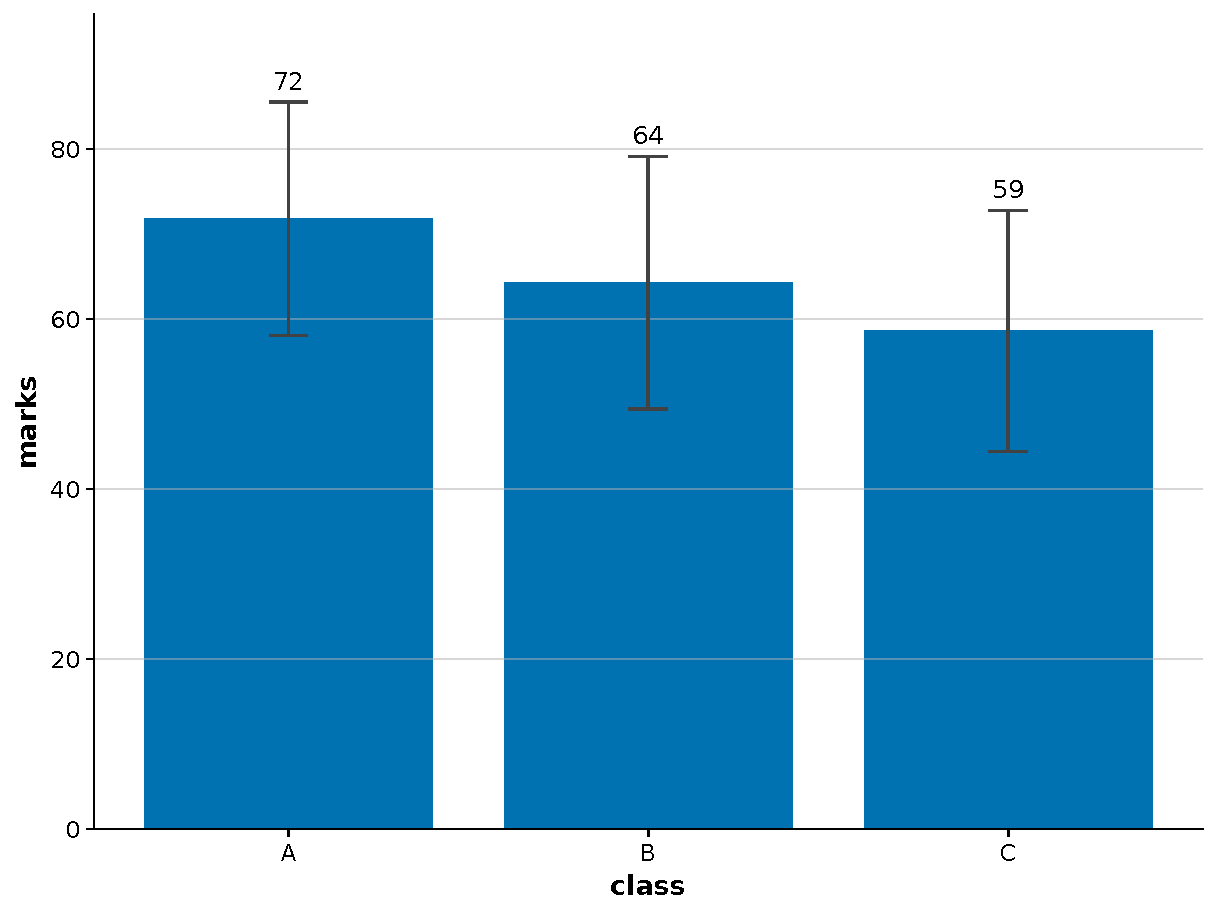
\includegraphics[width=0.72\textwidth,height=0.36\textheight,keepaspectratio]{figures/lesson05_example1_lesson5_average.pdf}
\captionof{figure}{Lesson 5, example 1: \code{lesson5\_\allowbreak{}average.\allowbreak{}png}.}
\end{minipage}\end{center}
\section*{Example 2}
A fit line is the straight line that goes as close as possible to all the dots.
\begin{lstlisting}[style=py]
import simplydata as sdata
marks = sdata.get_example("marks")
chart = sdata.chart(marks)
chart.draw_dots(x="hours", y="marks")
chart.fit_line(with_confidence_band=True, show_equation=True)
chart.save("lesson5_fit.png")
\end{lstlisting}
\whateachline
\begin{lineexplain}
  \item[1] Load simplydata.
  \item[2] Get the marks table.
  \item[3] Start a chart.
  \item[4] One dot per test: hours of study and the mark.
  \item[5] Add the best straight line (also called linear regression). \code{with\_\allowbreak{}confidence\_\allowbreak{}band=True} shades where the true line very likely is (the 95 \% confidence interval). \code{show\_\allowbreak{}equation=True} writes its equation and R\textsuperscript{2} (1 means the dots sit right on the line, 0 means no pattern at all).
  \item[6] Save it.
\end{lineexplain}
\printedoutput{output/lesson05_example2.txt}
\begin{center}\begin{minipage}{\linewidth}\centering
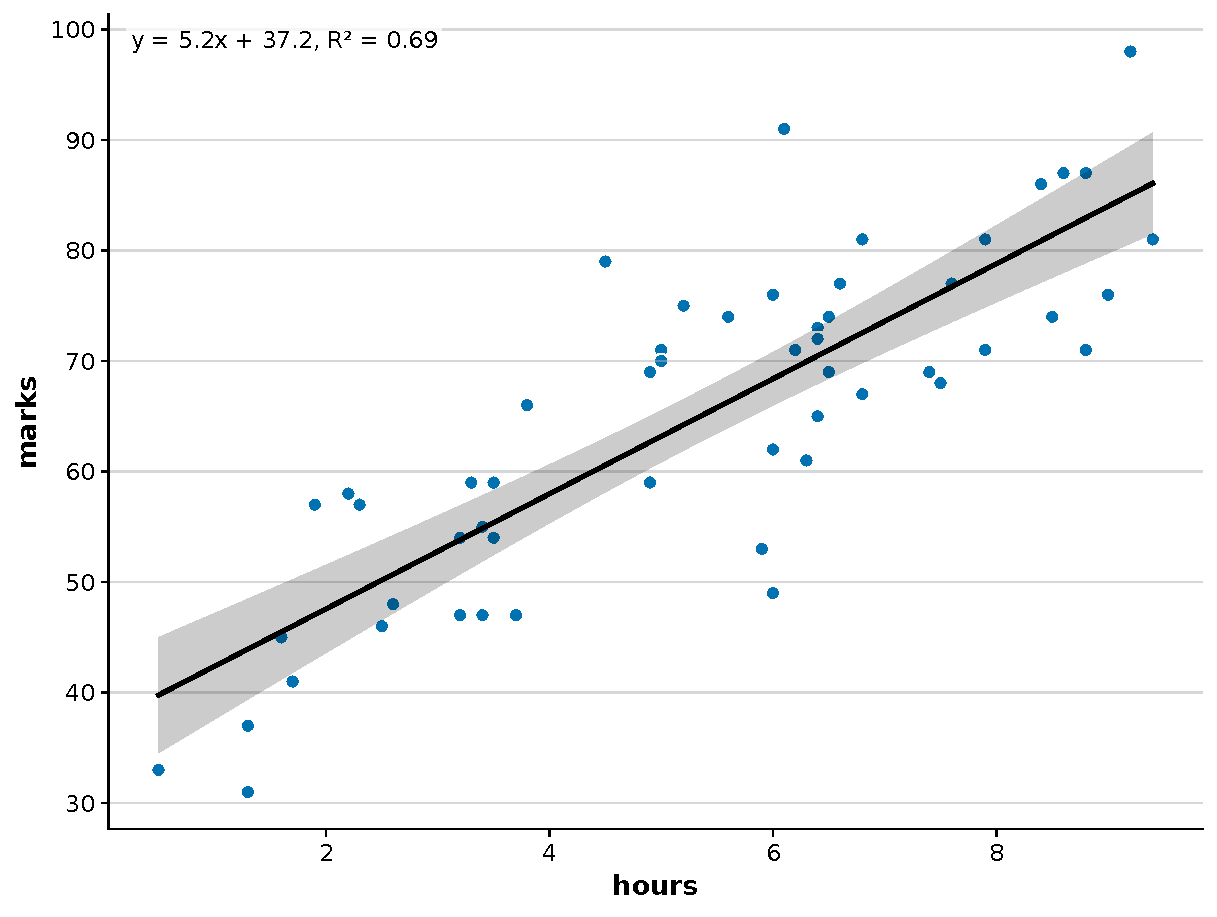
\includegraphics[width=0.72\textwidth,height=0.36\textheight,keepaspectratio]{figures/lesson05_example2_lesson5_fit.pdf}
\captionof{figure}{Lesson 5, example 2: \code{lesson5\_\allowbreak{}fit.\allowbreak{}png}.}
\end{minipage}\end{center}
\section*{Example 3}
A density curve is a smooth histogram: high where many values are.
\begin{lstlisting}[style=py]
import simplydata as sdata
marks = sdata.get_example("marks")
chart = sdata.chart(marks)
chart.draw_density(x="marks", colour="class")
chart.save("lesson5_density.png")
\end{lstlisting}
\whateachline
\begin{lineexplain}
  \item[1] Load simplydata.
  \item[2] Get the marks table.
  \item[3] Start a chart.
  \item[4] One smooth curve for each class (a kernel density estimate).
  \item[5] Save it.
\end{lineexplain}
\printedoutput{output/lesson05_example3.txt}
\begin{center}\begin{minipage}{\linewidth}\centering
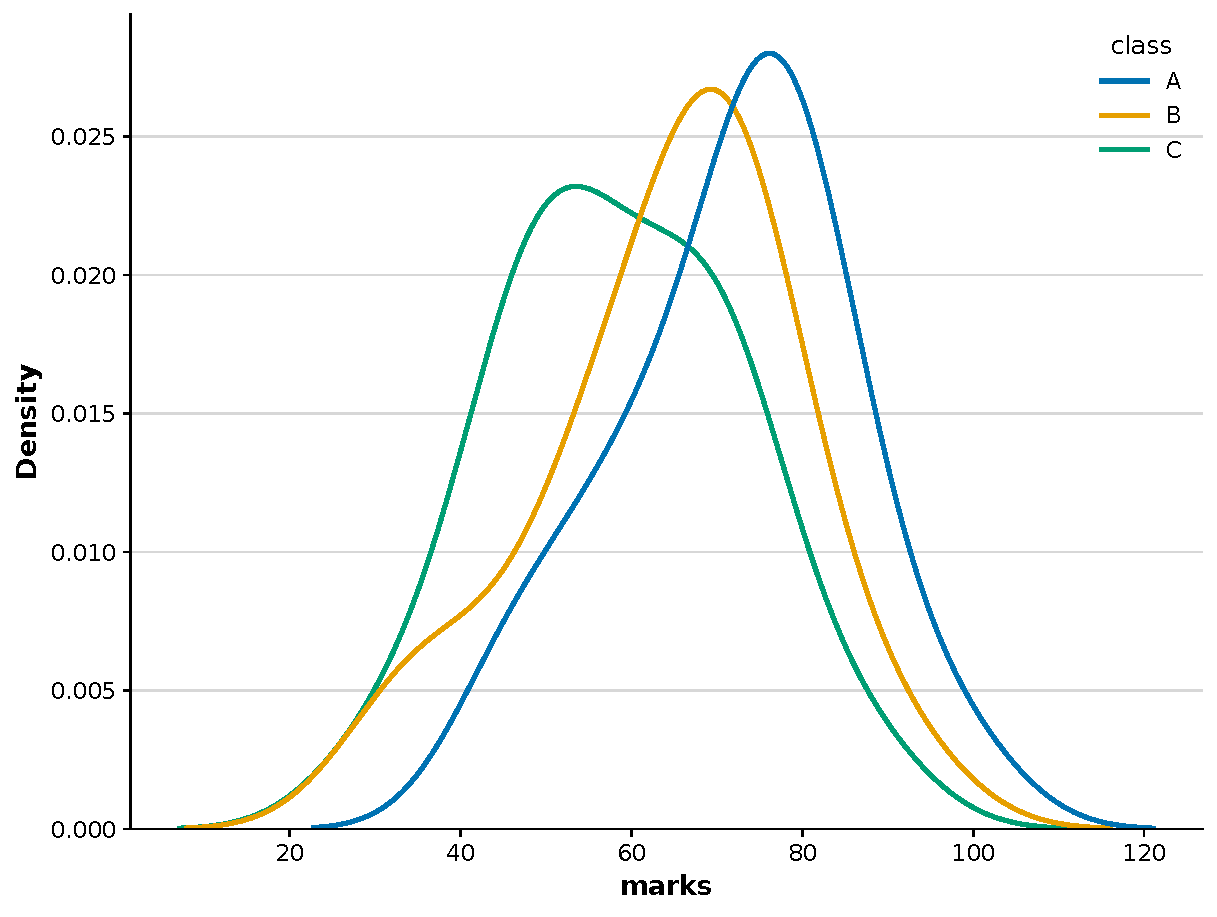
\includegraphics[width=0.72\textwidth,height=0.36\textheight,keepaspectratio]{figures/lesson05_example3_lesson5_density.pdf}
\captionof{figure}{Lesson 5, example 3: \code{lesson5\_\allowbreak{}density.\allowbreak{}png}.}
\end{minipage}\end{center}
\section*{Example 4}
Two more ways to see the shape of values: are they bell-shaped, and what share lies below each value?
\begin{lstlisting}[style=py]
import simplydata as sdata
marks = sdata.get_example("marks")
chart = sdata.chart(marks)
chart.draw_qq_dots("marks")
chart.save("lesson5_qq.png")
shares = sdata.chart(marks)
shares.draw_cumulative_share(x="marks", colour="class")
shares.save("lesson5_cumulative.png")
\end{lstlisting}
\whateachline
\begin{lineexplain}
  \item[1] Load simplydata.
  \item[2] Get the marks table.
  \item[3] Start a chart.
  \item[4] A Q-Q plot: if the marks follow a bell curve (normal), the dots lie close to the straight line.
  \item[5] Save it.
  \item[6] A second chart.
  \item[7] For each mark, the share of children with that mark or less (an ECDF). The class whose line is further right did better.
  \item[8] Save it.
\end{lineexplain}
\printedoutput{output/lesson05_example4.txt}
\begin{center}\begin{minipage}{\linewidth}\centering
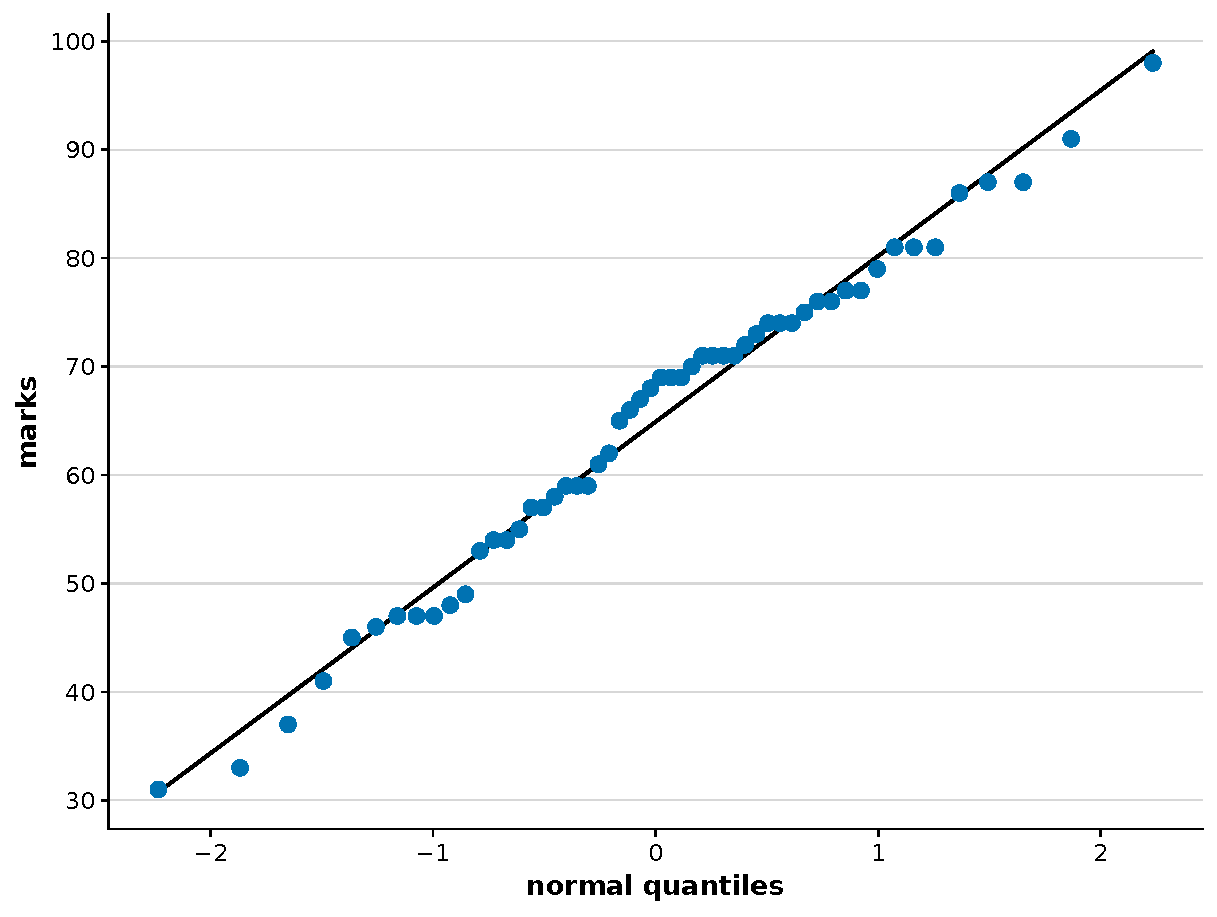
\includegraphics[width=0.48\textwidth,height=0.36\textheight,keepaspectratio]{figures/lesson05_example4_lesson5_qq.pdf}\hfill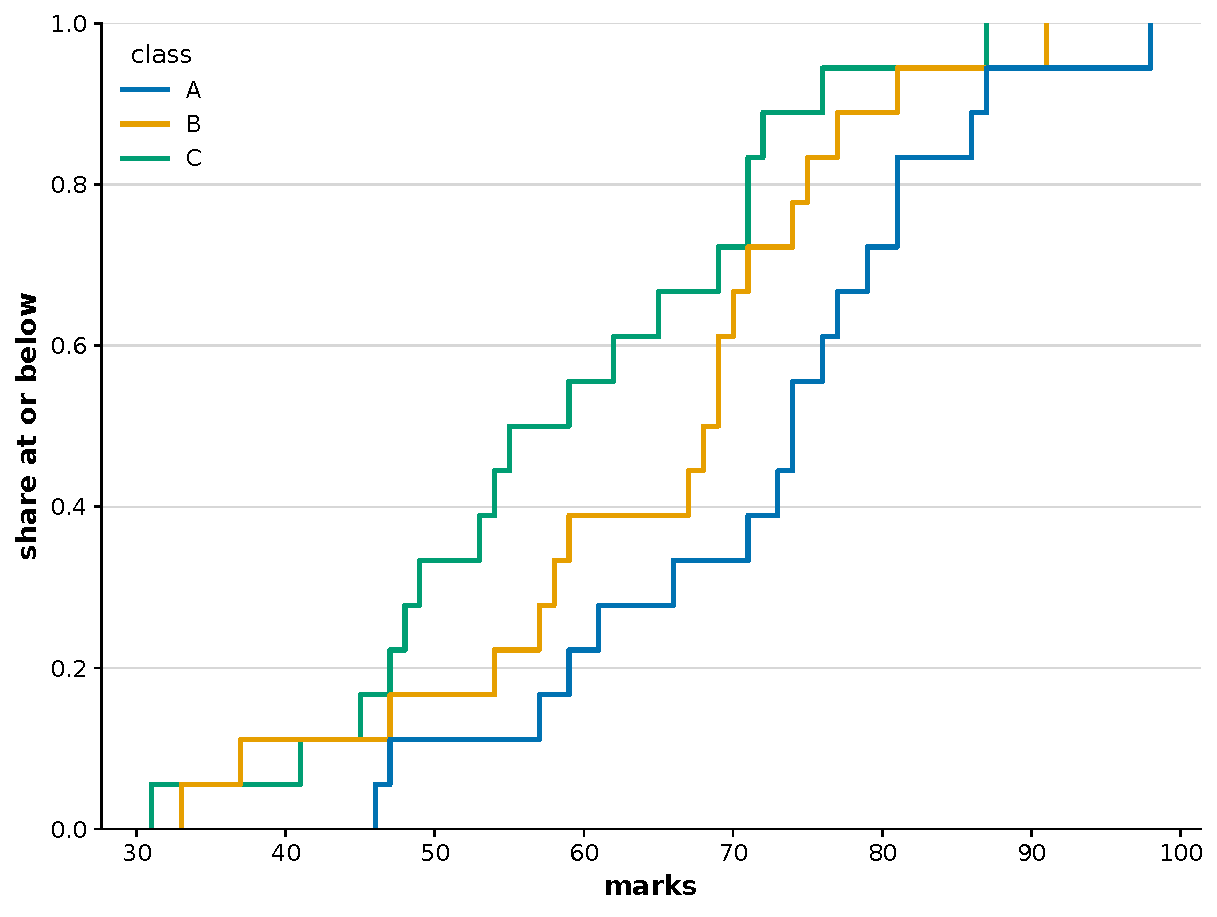
\includegraphics[width=0.48\textwidth,height=0.36\textheight,keepaspectratio]{figures/lesson05_example4_lesson5_cumulative.pdf}
\captionof{figure}{Lesson 5, example 4: \code{lesson5\_\allowbreak{}qq.\allowbreak{}png} and \code{lesson5\_\allowbreak{}cumulative.\allowbreak{}png}.}
\end{minipage}\end{center}
\begin{goodtoknow}
\begin{itemize}
  \item Average or median? The median is the middle value when the values are put in order. One very big or very small value pulls the average towards it, but hardly moves the median, so the median is safer when a few values are far from the rest (outliers).
  \item \code{show=} can be \code{\textquotedbl{}average\textquotedbl{}}, \code{\textquotedbl{}median\textquotedbl{}}, \code{\textquotedbl{}total\textquotedbl{}} (all added up), \code{\textquotedbl{}count\textquotedbl{}} (how many rows), \code{\textquotedbl{}smallest\textquotedbl{}}, \code{\textquotedbl{}biggest\textquotedbl{}} or \code{\textquotedbl{}standard deviation\textquotedbl{}}: the same names as the table words \code{find\_\allowbreak{}average\_\allowbreak{}of}, \code{find\_\allowbreak{}median\_\allowbreak{}of} and so on.
  \item Standard deviation or standard error? The standard deviation describes the values: how spread out they are. The standard error describes the average: how sure we are of it. It gets smaller as you collect more values, even when the values spread just as much.
  \item \code{error=\textquotedbl{}confidence interval\textquotedbl{}} draws the 95 \% confidence interval: the range the true average is very likely to be in. The short forms \code{\textquotedbl{}sd\textquotedbl{}}, \code{\textquotedbl{}se\textquotedbl{}} and \code{\textquotedbl{}ci\textquotedbl{}} work too. Always say in your caption which error bars you drew.
  \item \code{fit\_\allowbreak{}curve(of\_\allowbreak{}degree=2)} fits a curve with one bend; \code{draw\_\allowbreak{}smooth\_\allowbreak{}line()} follows the dots freely.
\end{itemize}
\end{goodtoknow}
\begin{tryit}
\begin{enumerate}
  \item Change \code{show=\textquotedbl{}average\textquotedbl{}} to \code{show=\textquotedbl{}median\textquotedbl{}}. Do the bars change much?
  \item Change \code{error=\textquotedbl{}standard deviation\textquotedbl{}} to \code{error=\textquotedbl{}standard error\textquotedbl{}}. Are the error bars bigger or smaller? Why?
  \item Make a chart of the weather table, draw dots with \code{x=\textquotedbl{}month\_\allowbreak{}number\textquotedbl{}}, \code{y=\textquotedbl{}temperature\textquotedbl{}} and add \code{chart.\allowbreak{}fit\_\allowbreak{}curve(of\_\allowbreak{}degree=2)}.
\end{enumerate}
Worked solutions: page~\pageref{solutions:5}, or type \code{sdata.\allowbreak{}show\_\allowbreak{}lesson(5,\allowbreak{} solutions=True)}.
\end{tryit}
\par\noindent{\small\sffamily\textbf{Words in this lesson:} \hyperref[word:show-eq]{\code{show=}}, \hyperref[word:error-eq]{\code{error=}}, \hyperref[word:write-numbers-on-bars]{\code{chart.\allowbreak{}write\_\allowbreak{}numbers\_\allowbreak{}on\_\allowbreak{}bars()}}, \hyperref[word:fit-line]{\code{chart.\allowbreak{}fit\_\allowbreak{}line()}}, \hyperref[word:draw-density]{\code{chart.\allowbreak{}draw\_\allowbreak{}density()}}, \hyperref[word:fit-curve]{\code{chart.\allowbreak{}fit\_\allowbreak{}curve()}}, \hyperref[word:draw-smooth-line]{\code{chart.\allowbreak{}draw\_\allowbreak{}smooth\_\allowbreak{}line()}}, \hyperref[word:draw-qq-dots]{\code{chart.\allowbreak{}draw\_\allowbreak{}qq\_\allowbreak{}dots()}}, \hyperref[word:draw-cumulative-share]{\code{chart.\allowbreak{}draw\_\allowbreak{}cumulative\_\allowbreak{}share()}}.\par}

\chapter{Axes and reference lines}\label{lesson:6}
\begin{learnbox}
\begin{itemize}
  \item how to choose where an axis starts and stops
  \item how to draw a line at a value, like a pass mark, and shade a band
  \item how to choose the tick marks, and what a log scale is
\end{itemize}
\end{learnbox}
\section*{Example 1}
The axes are the two edges with numbers: x along the bottom, y up the side.
\begin{lstlisting}[style=py]
import simplydata as sdata
marks = sdata.get_example("marks")
chart = sdata.chart(marks)
chart.draw_bars(x="name", y="marks")
chart.set_range_y(0, 100)
chart.put_ticks_y(0, 25, 50, 75, 100)
chart.draw_line_at_y(50, labelled="pass mark")
chart.shade_between_y(40, 60)
chart.rotate_labels_x()
chart.save("lesson6_marks.png")
\end{lstlisting}
\whateachline
\begin{lineexplain}
  \item[1] Load simplydata.
  \item[2] Get the marks table.
  \item[3] Start a chart.
  \item[4] One bar for each child.
  \item[5] Make the y-axis go from 0 to 100, the lowest and highest mark you can get.
  \item[6] Put the numbers on the y-axis at these places.
  \item[7] Draw a dashed line across at 50, with a name.
  \item[8] Shade the band between 40 and 60.
  \item[9] Turn the names so they fit.
  \item[10] Save it.
\end{lineexplain}
\printedoutput{output/lesson06_example1.txt}
\begin{center}\begin{minipage}{\linewidth}\centering
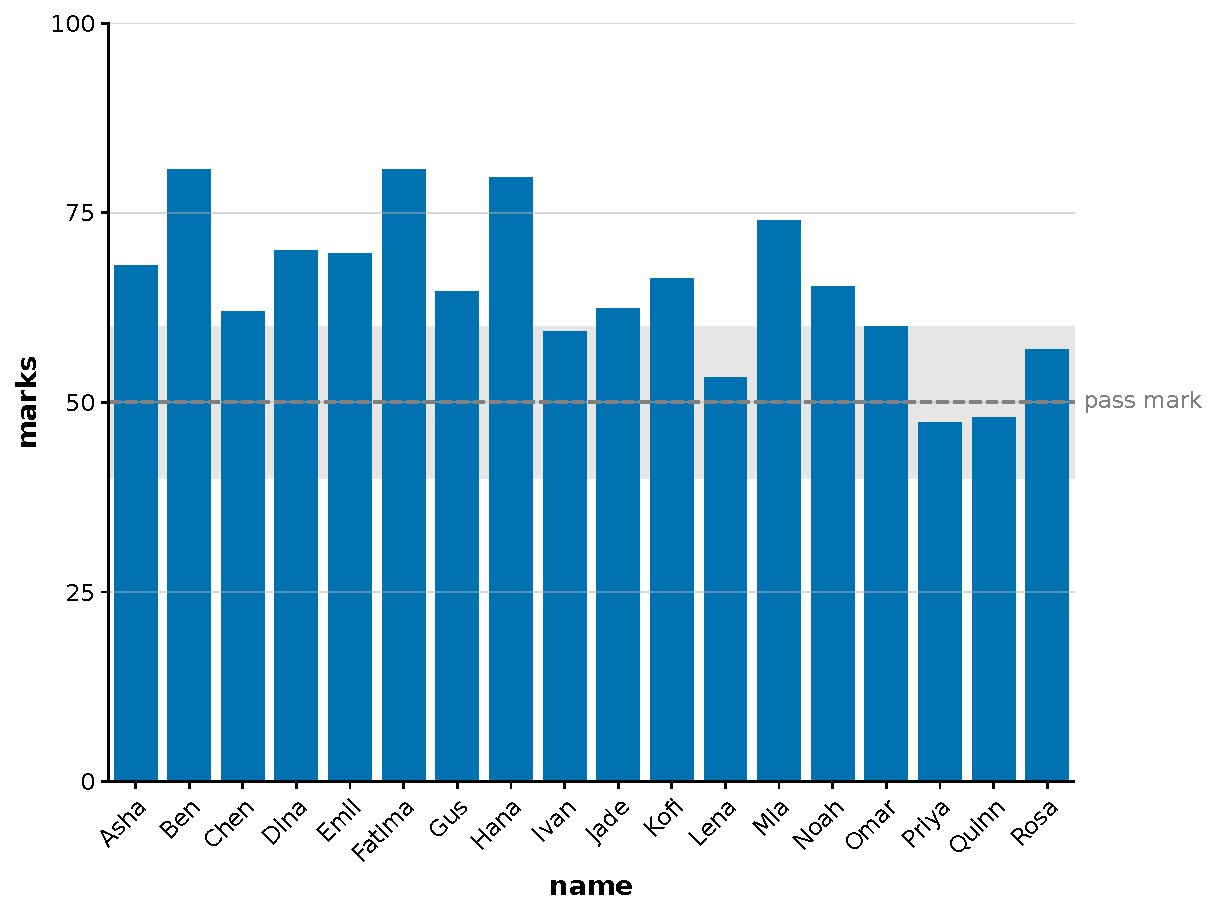
\includegraphics[width=0.72\textwidth,height=0.36\textheight,keepaspectratio]{figures/lesson06_example1_lesson6_marks.pdf}
\captionof{figure}{Lesson 6, example 1: \code{lesson6\_\allowbreak{}marks.\allowbreak{}png}.}
\end{minipage}\end{center}
\section*{Example 2}
On a log scale 1, 10, 100 and 1000 are the same distance apart. It helps when some numbers are much bigger than others.
\begin{lstlisting}[style=py]
import simplydata as sdata
growth = sdata.get_example("growth")
chart = sdata.chart(growth)
chart.draw_lines(x="year", y="population", colour="country")
chart.use_log_scale_y()
chart.draw_line_at_x(2010, labelled="2010")
chart.label_y("People (millions)")
chart.save("lesson6_log.png")
\end{lstlisting}
\whateachline
\begin{lineexplain}
  \item[1] Load simplydata.
  \item[2] Get the growth table: people in four made-up countries.
  \item[3] Start a chart.
  \item[4] One line per country.
  \item[5] Use a log scale on the y-axis. A country that grows by the same share each year now gets a straight line.
  \item[6] Draw an up-and-down line at the year 2010.
  \item[7] Name the y-axis.
  \item[8] Save it.
\end{lineexplain}
\printedoutput{output/lesson06_example2.txt}
\begin{center}\begin{minipage}{\linewidth}\centering
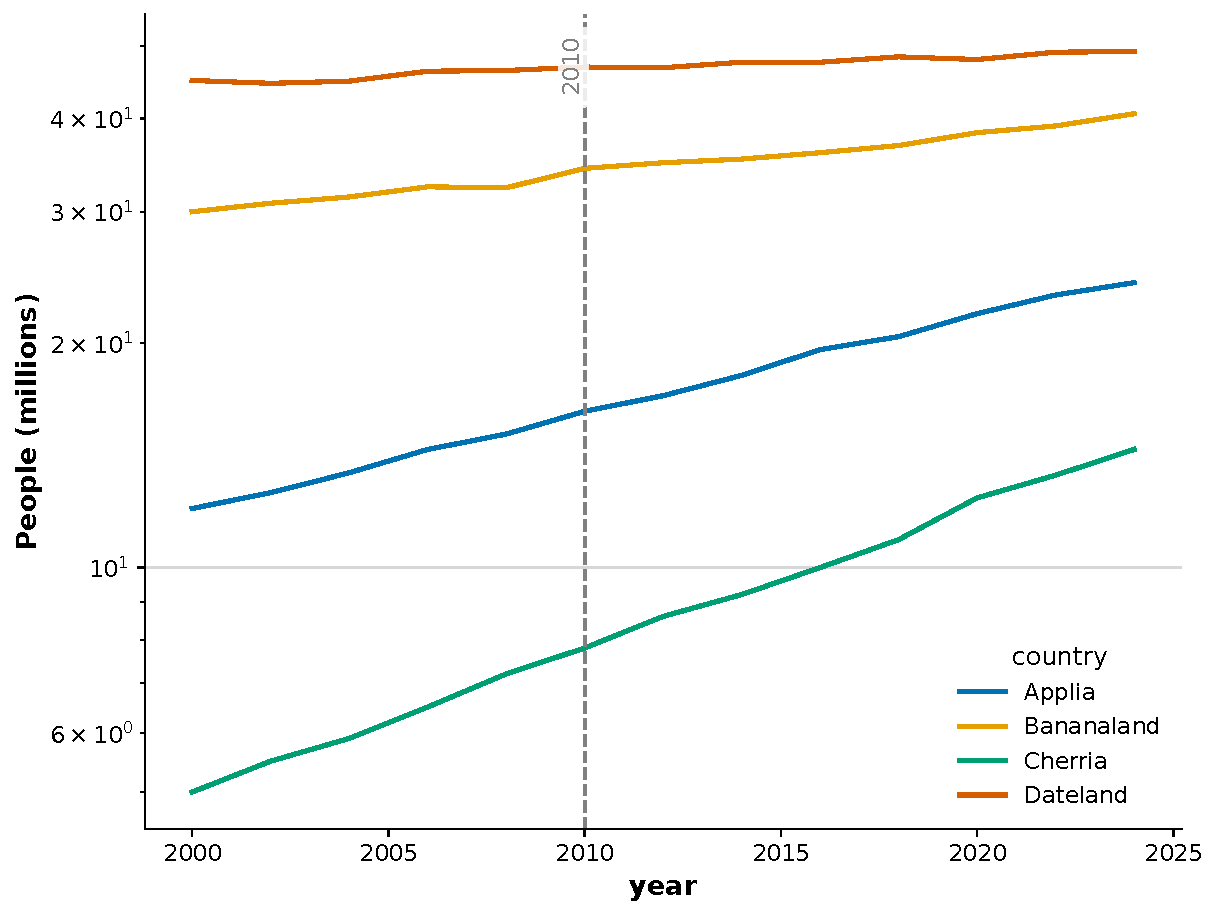
\includegraphics[width=0.72\textwidth,height=0.36\textheight,keepaspectratio]{figures/lesson06_example2_lesson6_log.pdf}
\captionof{figure}{Lesson 6, example 2: \code{lesson6\_\allowbreak{}log.\allowbreak{}png}.}
\end{minipage}\end{center}
\section*{Example 3}
A band shades the space between a low and a high value at each x: a range, or the uncertainty around a line.
\begin{lstlisting}[style=py]
import simplydata as sdata
days = {"day": [1, 2, 3, 4, 5], "lowest": [3, 5, 4, 6, 8], "average": [6, 8, 7, 9, 11], "highest": [9, 11, 10, 12, 14]}
chart = sdata.chart(days)
chart.draw_band(x="day", between=["lowest", "highest"], labelled="lowest to highest")
chart.draw_lines(x="day", y="average")
chart.label_y("Temperature (°C)")
chart.save("lesson6_band.png")
\end{lstlisting}
\whateachline
\begin{lineexplain}
  \item[1] Load simplydata.
  \item[2] A small table: the lowest, average and highest temperature on five days.
  \item[3] Start a chart of it.
  \item[4] Shade from the lowest to the highest value of each day. \code{labelled=} names it in the legend.
  \item[5] The average as a line through the band.
  \item[6] Name the y-axis.
  \item[7] Save it.
\end{lineexplain}
\printedoutput{output/lesson06_example3.txt}
\begin{center}\begin{minipage}{\linewidth}\centering
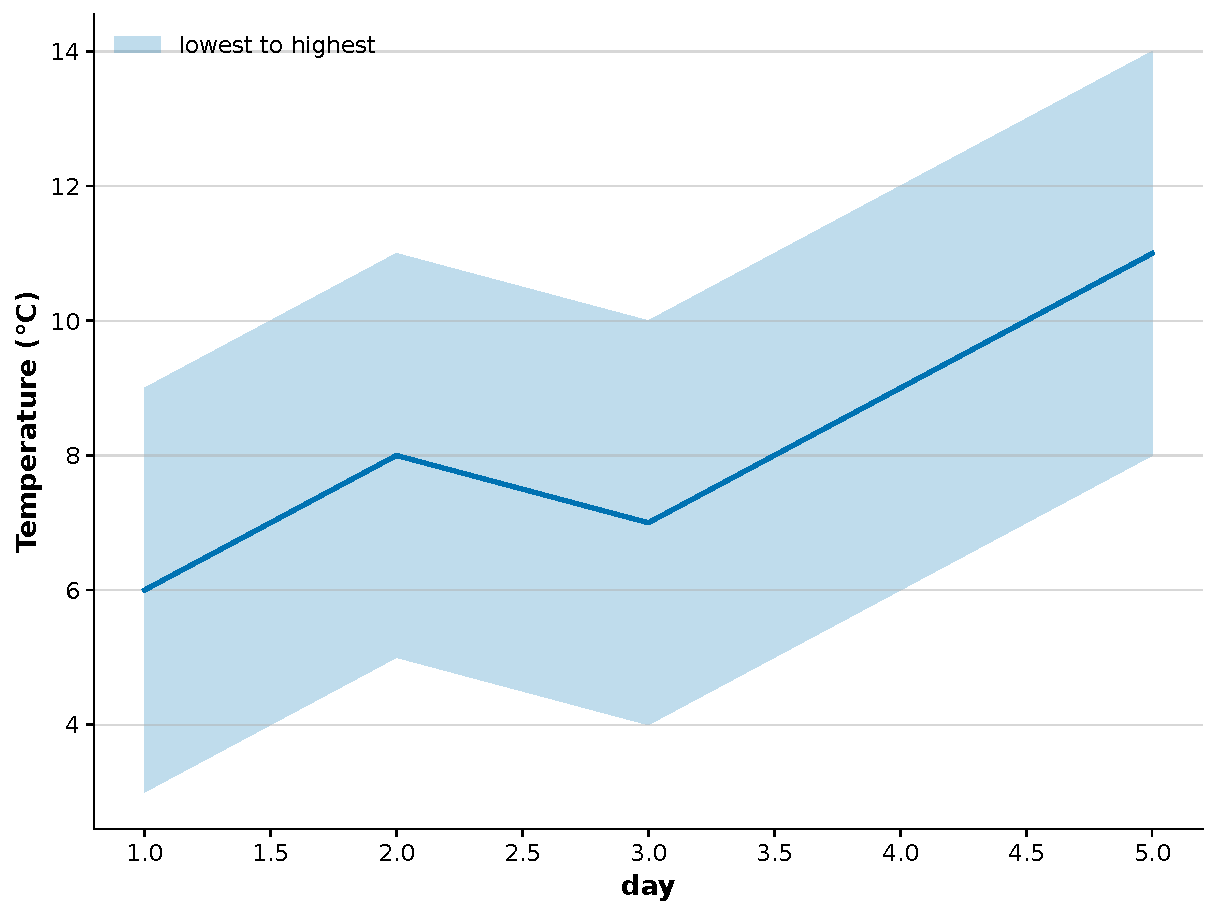
\includegraphics[width=0.72\textwidth,height=0.36\textheight,keepaspectratio]{figures/lesson06_example3_lesson6_band.pdf}
\captionof{figure}{Lesson 6, example 3: \code{lesson6\_\allowbreak{}band.\allowbreak{}png}.}
\end{minipage}\end{center}
\section*{Example 4}
Axes can say what their numbers mean, and a 1:1 line shows where two columns agree.
\begin{lstlisting}[style=py]
import simplydata as sdata
growth = sdata.get_example("growth")
chart = sdata.chart(growth)
chart.draw_lines(x="year", y="forest", colour="country")
chart.write_ticks_y_as("percent")
chart.save("lesson6_percent.png")
guesses = {"measured": [12, 18, 25, 31, 40], "predicted": [14, 17, 27, 29, 43]}
check = sdata.chart(guesses)
check.draw_dots(x="measured", y="predicted")
check.draw_line_with_slope(1, through=(0, 0), labelled="1:1")
check.save("lesson6_one_to_one.png")
\end{lstlisting}
\whateachline
\begin{lineexplain}
  \item[1] Load simplydata.
  \item[2] Get the growth table.
  \item[3] Start a chart.
  \item[4] The forest of each country, in \%.
  \item[5] Write the y numbers as 40 \%, 50 \% ... (\code{\textquotedbl{}thousands\textquotedbl{}}, \code{\textquotedbl{}scientific\textquotedbl{}} and dates such as \code{\textquotedbl{}Jan 2026\textquotedbl{}} work too).
  \item[6] Save it.
  \item[7] Five measured values and what a model predicted for them.
  \item[8] A second chart.
  \item[9] One dot per value.
  \item[10] The 1:1 line: dots on it were predicted exactly; above it, too high.
  \item[11] Save it.
\end{lineexplain}
\printedoutput{output/lesson06_example4.txt}
\begin{center}\begin{minipage}{\linewidth}\centering
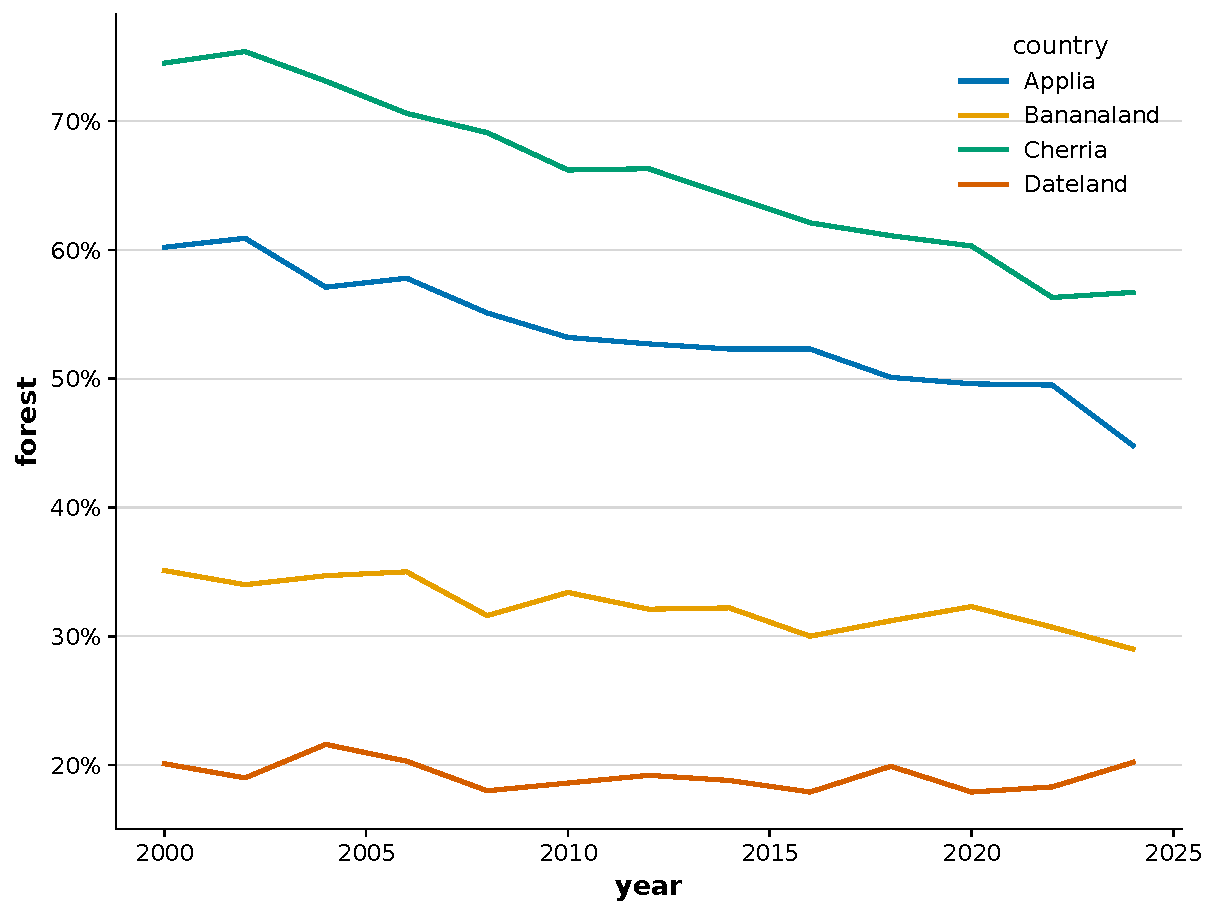
\includegraphics[width=0.48\textwidth,height=0.36\textheight,keepaspectratio]{figures/lesson06_example4_lesson6_percent.pdf}\hfill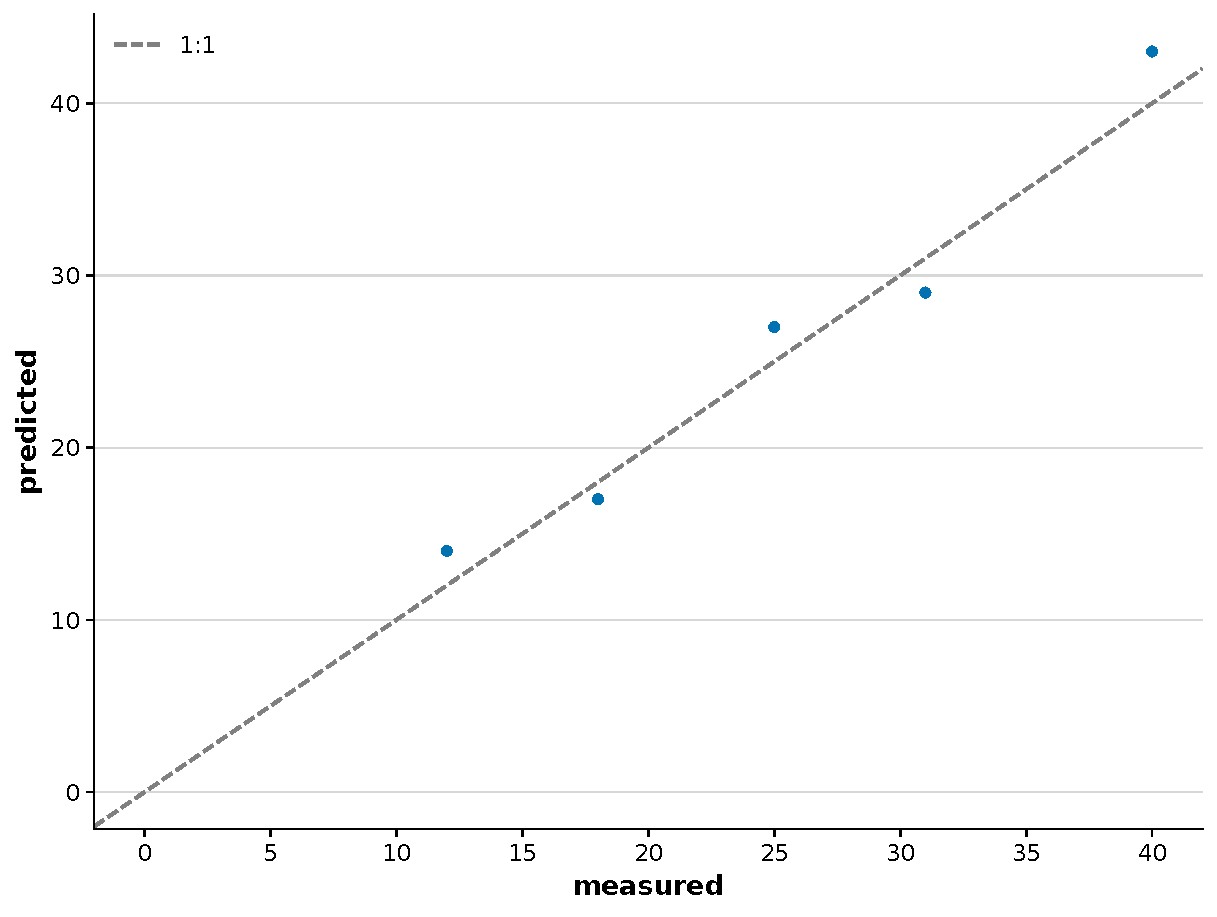
\includegraphics[width=0.48\textwidth,height=0.36\textheight,keepaspectratio]{figures/lesson06_example4_lesson6_one_to_one.pdf}
\captionof{figure}{Lesson 6, example 4: \code{lesson6\_\allowbreak{}percent.\allowbreak{}png} and \code{lesson6\_\allowbreak{}one\_\allowbreak{}to\_\allowbreak{}one.\allowbreak{}png}.}
\end{minipage}\end{center}
\begin{goodtoknow}
\begin{itemize}
  \item Every axis word ends in \_x or \_y: \code{set\_\allowbreak{}range\_\allowbreak{}x}, \code{put\_\allowbreak{}ticks\_\allowbreak{}x}, \code{use\_\allowbreak{}log\_\allowbreak{}scale\_\allowbreak{}x}, \code{draw\_\allowbreak{}line\_\allowbreak{}at\_\allowbreak{}x}, \code{shade\_\allowbreak{}between\_\allowbreak{}x}, \code{flip\_\allowbreak{}x} ...
  \item \code{set\_\allowbreak{}range\_\allowbreak{}y(0,\allowbreak{} None)} fixes only the bottom and lets the top choose itself.
  \item Bars should start at 0: a bar is read by its length, so a y-axis that starts at 40 makes small differences look big.
\end{itemize}
\end{goodtoknow}
\begin{tryit}
\begin{enumerate}
  \item Move the pass mark to 60 and shade between 0 and 40 instead.
  \item Take away \code{chart.\allowbreak{}use\_\allowbreak{}log\_\allowbreak{}scale\_\allowbreak{}y()}. Which countries look different?
  \item Try \code{chart.\allowbreak{}flip\_\allowbreak{}y()} on any chart. What happens?
\end{enumerate}
Worked solutions: page~\pageref{solutions:6}, or type \code{sdata.\allowbreak{}show\_\allowbreak{}lesson(6,\allowbreak{} solutions=True)}.
\end{tryit}
\par\noindent{\small\sffamily\textbf{Words in this lesson:} \hyperref[word:set-range-y]{\code{chart.\allowbreak{}set\_\allowbreak{}range\_\allowbreak{}y()}}, \hyperref[word:put-ticks-y]{\code{chart.\allowbreak{}put\_\allowbreak{}ticks\_\allowbreak{}y()}}, \hyperref[word:draw-line-at-y]{\code{chart.\allowbreak{}draw\_\allowbreak{}line\_\allowbreak{}at\_\allowbreak{}y()}}, \hyperref[word:shade-between-y]{\code{chart.\allowbreak{}shade\_\allowbreak{}between\_\allowbreak{}y()}}, \hyperref[word:use-log-scale-y]{\code{chart.\allowbreak{}use\_\allowbreak{}log\_\allowbreak{}scale\_\allowbreak{}y()}}, \hyperref[word:draw-line-at-x]{\code{chart.\allowbreak{}draw\_\allowbreak{}line\_\allowbreak{}at\_\allowbreak{}x()}}, \hyperref[word:flip-y]{\code{chart.\allowbreak{}flip\_\allowbreak{}y()}}, \hyperref[word:draw-band]{\code{chart.\allowbreak{}draw\_\allowbreak{}band()}}, \hyperref[word:write-ticks-y-as]{\code{chart.\allowbreak{}write\_\allowbreak{}ticks\_\allowbreak{}y\_\allowbreak{}as()}}, \hyperref[word:draw-line-with-slope]{\code{chart.\allowbreak{}draw\_\allowbreak{}line\_\allowbreak{}with\_\allowbreak{}slope()}}.\par}

\chapter{Several charts together}\label{lesson:7}
\begin{learnbox}
\begin{itemize}
  \item how to make one small chart for each group
  \item how to put different charts on one page: side by side, one above the other, or in a grid
  \item how to write A, B, C on the charts, as figures in papers have
  \item how to compare every number column with every other
\end{itemize}
\end{learnbox}
\section*{Example 1}
\code{draw\_\allowbreak{}one\_\allowbreak{}chart\_\allowbreak{}for\_\allowbreak{}each\_\allowbreak{}group\_\allowbreak{}in} draws the same chart once for each group.
\begin{lstlisting}[style=py]
import simplydata as sdata
marks = sdata.get_example("marks")
chart = sdata.chart(marks)
chart.draw_dots(x="hours", y="marks")
chart.fit_line()
chart.draw_one_chart_for_each_group_in("class")
chart.save("lesson7_one_chart_per.png")
\end{lstlisting}
\whateachline
\begin{lineexplain}
  \item[1] Load simplydata.
  \item[2] Get the marks table.
  \item[3] Start a chart.
  \item[4] Dots of hours and marks.
  \item[5] Add a fit line.
  \item[6] Make one small chart for each class, with the same axes so they are easy to compare.
  \item[7] Save it.
\end{lineexplain}
\printedoutput{output/lesson07_example1.txt}
\begin{center}\begin{minipage}{\linewidth}\centering
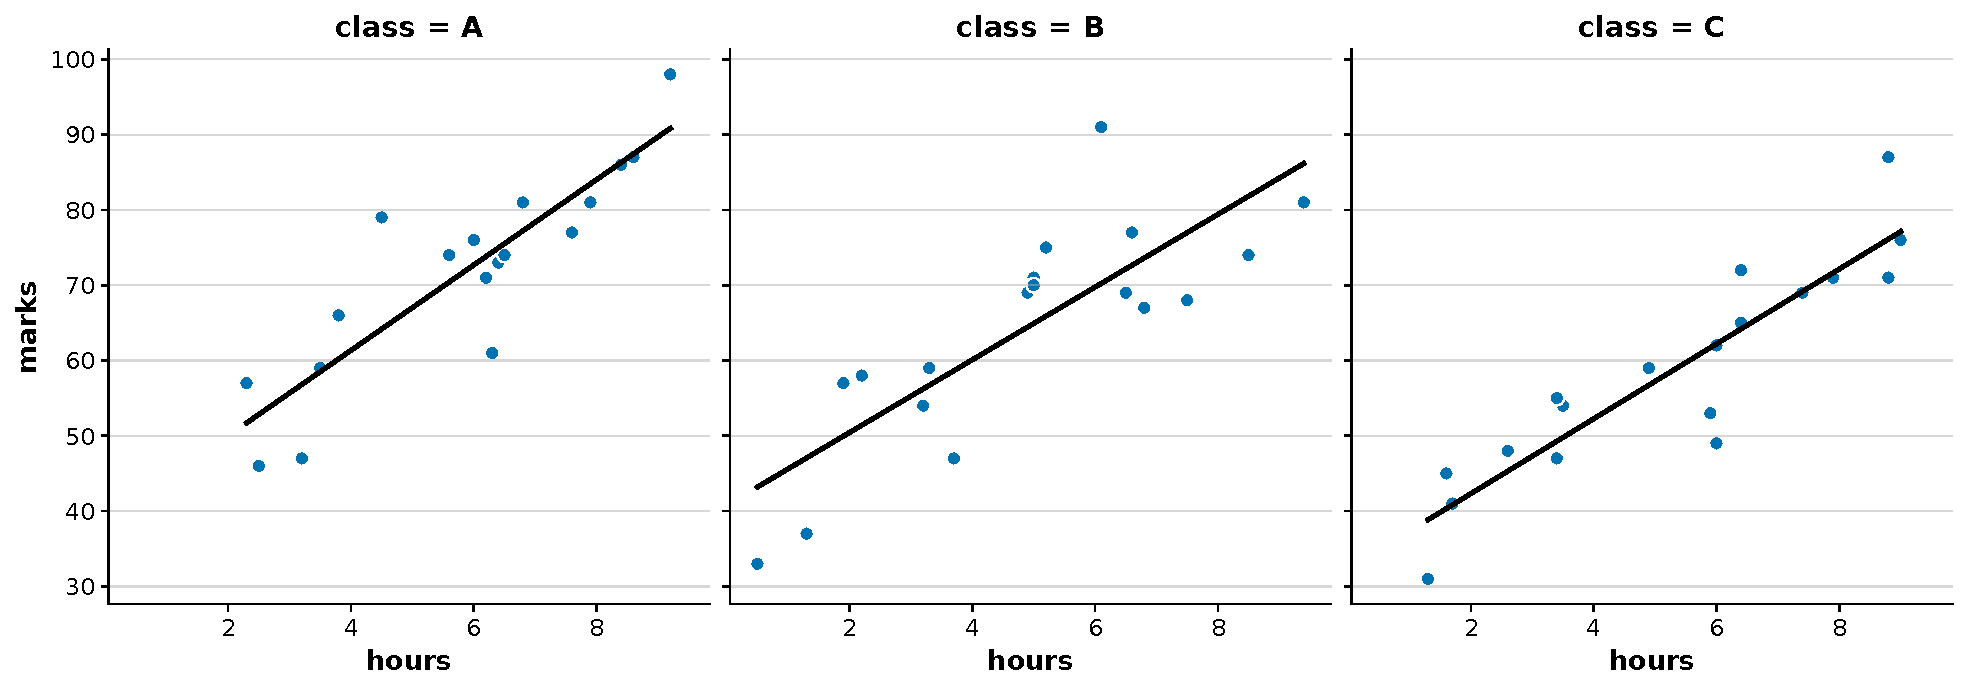
\includegraphics[width=0.72\textwidth,height=0.36\textheight,keepaspectratio]{figures/lesson07_example1_lesson7_one_chart_per.pdf}
\captionof{figure}{Lesson 7, example 1: \code{lesson7\_\allowbreak{}one\_\allowbreak{}chart\_\allowbreak{}per.\allowbreak{}png}.}
\end{minipage}\end{center}
\section*{Example 2}
Each chart is an object of its own, so different charts can share one page.
\begin{lstlisting}[style=py]
import simplydata as sdata
weather = sdata.get_example("weather")
a = sdata.chart(weather).draw_lines(x="month", y="temperature", colour="city")
b = sdata.chart(weather).draw_bars(x="month", y="rain", colour="city")
page = sdata.put_one_above_other(a, b)
page.write_title_on_top("A year of weather")
page.save("lesson7_page.png")
\end{lstlisting}
\whateachline
\begin{lineexplain}
  \item[1] Load simplydata.
  \item[2] Get the weather table.
  \item[3] Make a first chart, called a. Steps can also be joined with dots on one line.
  \item[4] Make a second chart, called b.
  \item[5] Put a above b on one page.
  \item[6] Give the whole page a title.
  \item[7] Save the page.
\end{lineexplain}
\printedoutput{output/lesson07_example2.txt}
\begin{center}\begin{minipage}{\linewidth}\centering
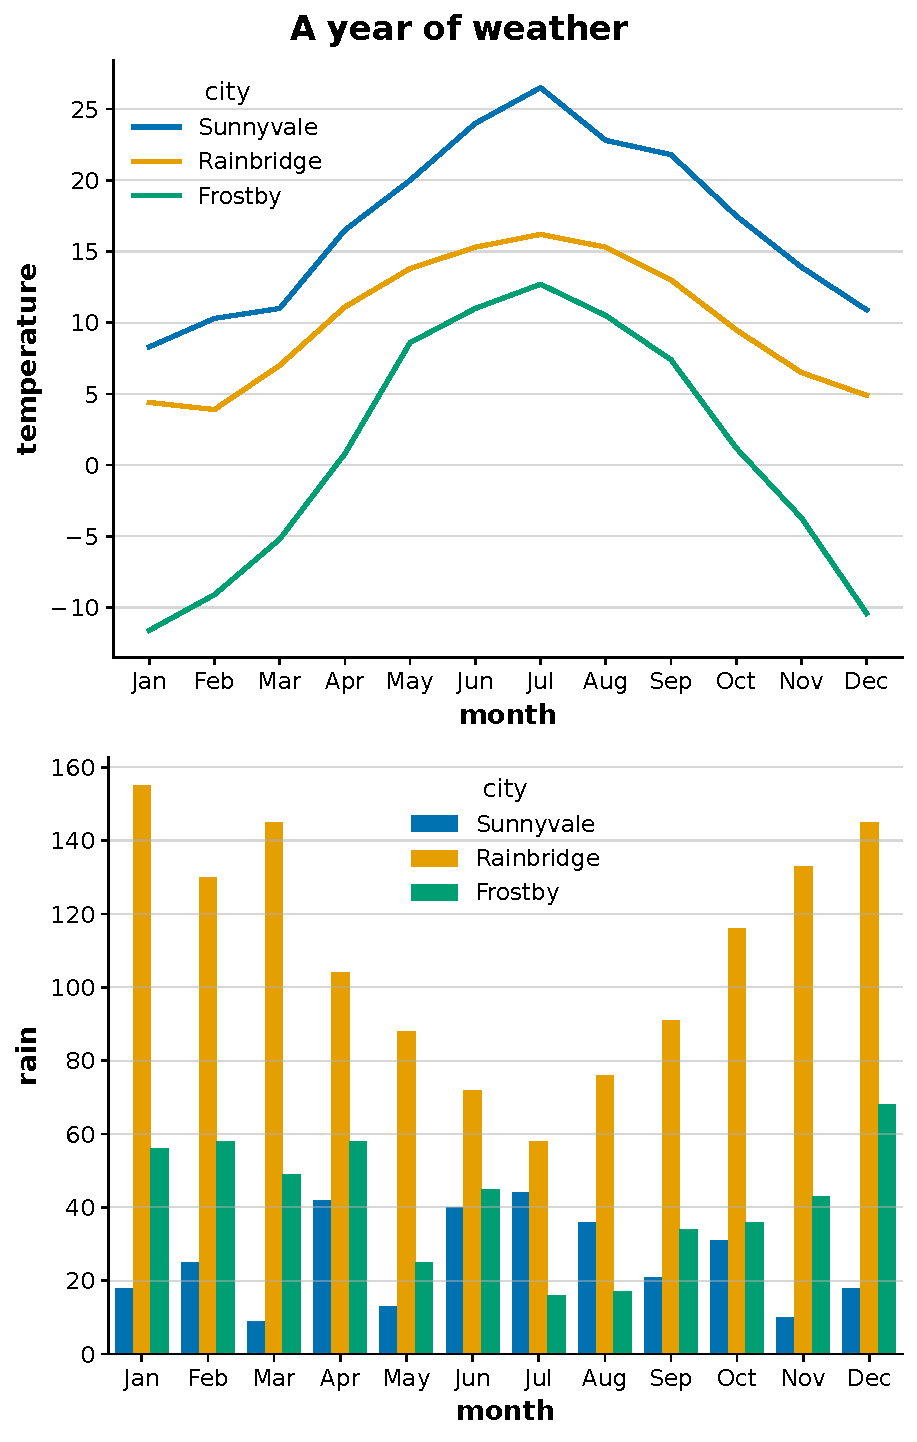
\includegraphics[width=0.72\textwidth,height=0.36\textheight,keepaspectratio]{figures/lesson07_example2_lesson7_page.pdf}
\captionof{figure}{Lesson 7, example 2: \code{lesson7\_\allowbreak{}page.\allowbreak{}png}.}
\end{minipage}\end{center}
\section*{Example 3}
A grid holds many charts in rows and columns. \code{with\_\allowbreak{}letters=True} writes A, B, C and D on them, as figures in papers have.
\begin{lstlisting}[style=py]
import simplydata as sdata
marks = sdata.get_example("marks")
a = sdata.chart(marks).draw_bars(x="class", y="marks").write_title_on_top("Average")
b = sdata.chart(marks).draw_histogram(x="marks").write_title_on_top("All marks")
c = sdata.chart(marks).draw_dots(x="height", y="marks").write_title_on_top("Height")
d = sdata.chart(marks).draw_boxes(x="subject", y="marks").write_title_on_top("Subjects")
page = sdata.put_in_rows_and_columns(a, b, c, d, per_row=2, with_letters=True)
page.save("lesson7_grid.png")
\end{lstlisting}
\whateachline
\begin{lineexplain}
  \item[1] Load simplydata.
  \item[2] Get the marks table.
  \item[3] Chart a.
  \item[4] Chart b.
  \item[5] Chart c.
  \item[6] Chart d.
  \item[7] All four in a grid, 2 charts per row, with a letter on each.
  \item[8] Save it.
\end{lineexplain}
\printedoutput{output/lesson07_example3.txt}
\begin{center}\begin{minipage}{\linewidth}\centering
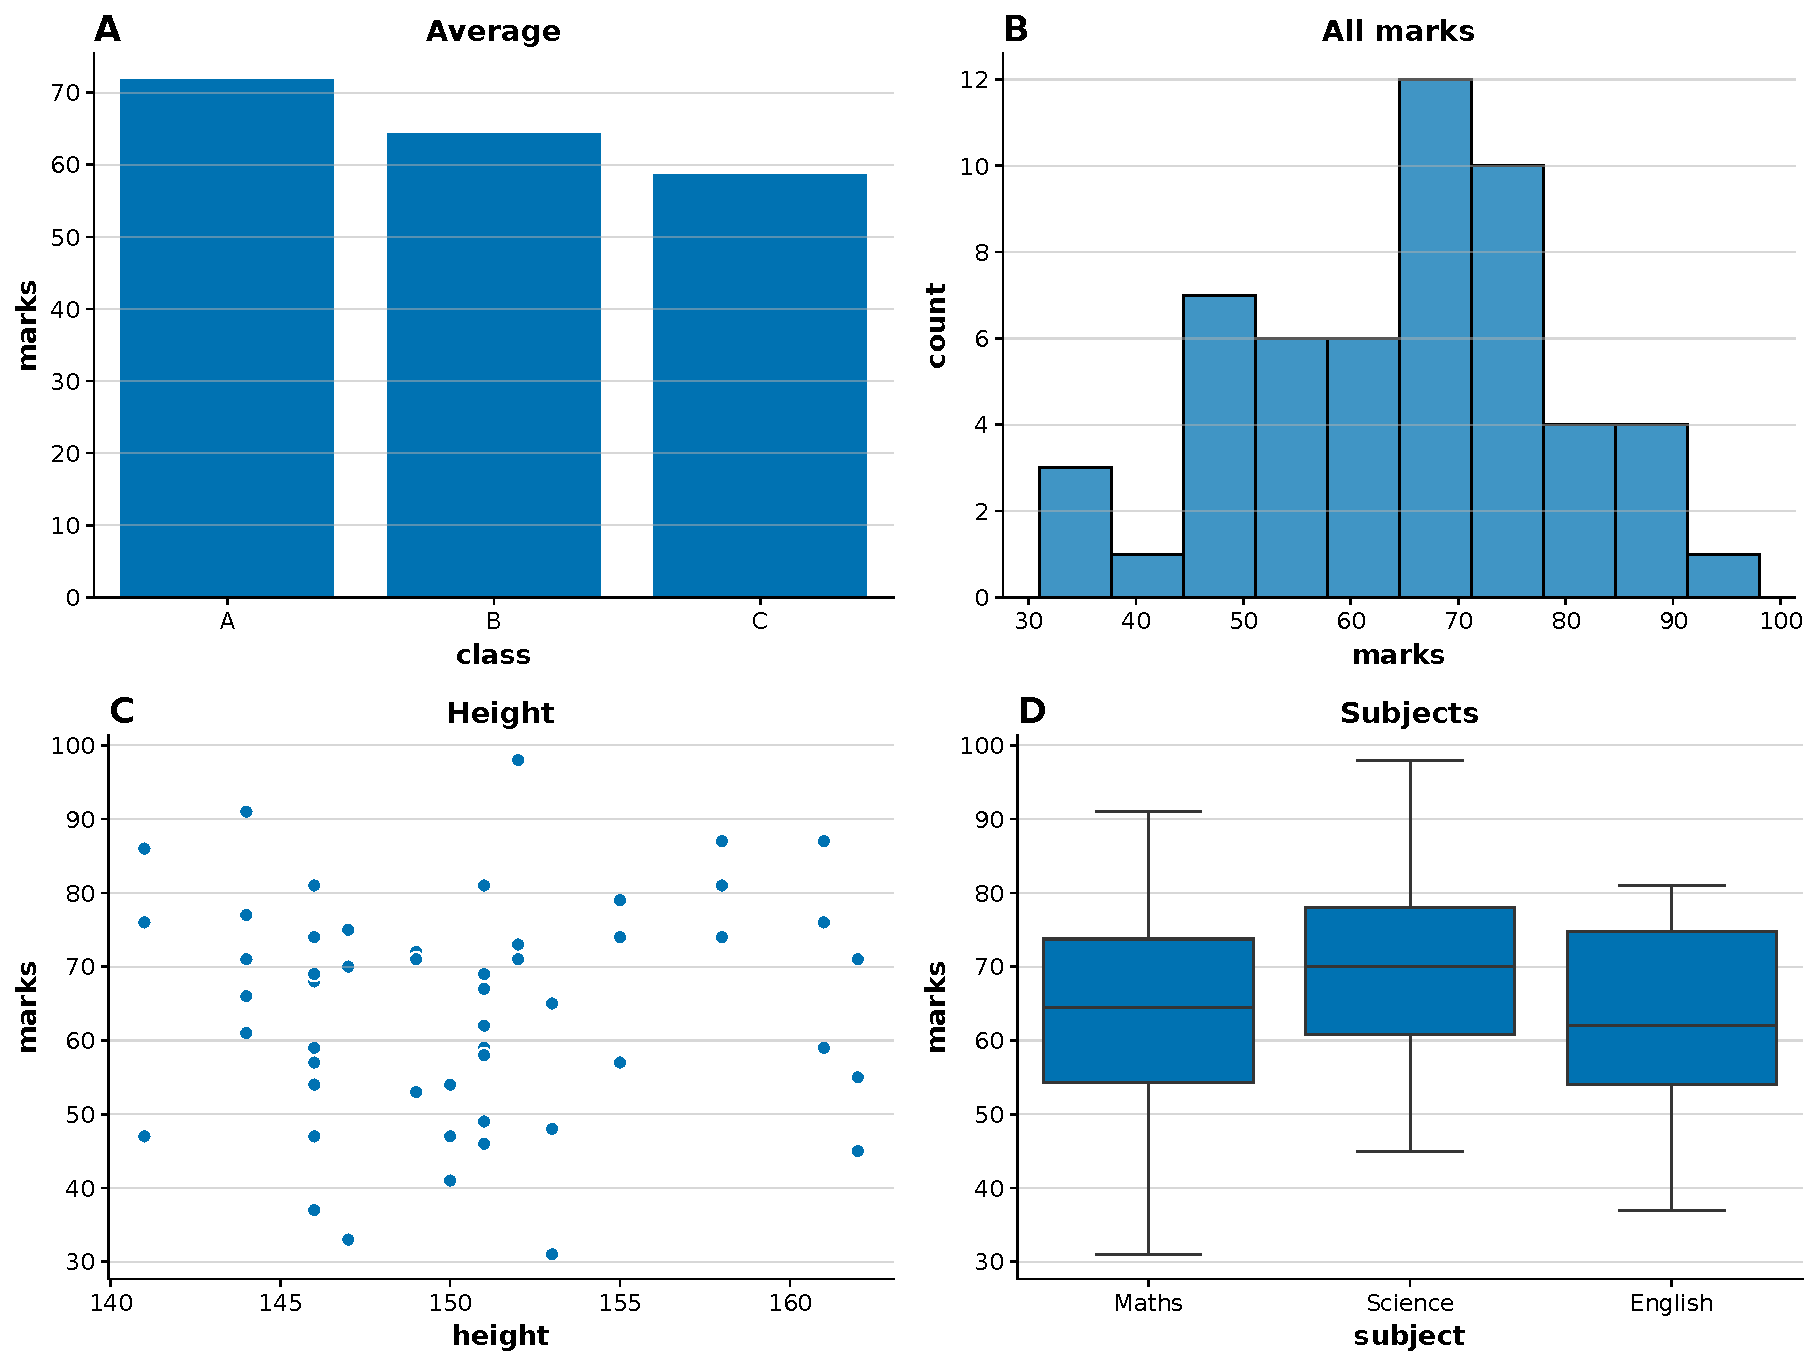
\includegraphics[width=0.72\textwidth,height=0.36\textheight,keepaspectratio]{figures/lesson07_example3_lesson7_grid.pdf}
\captionof{figure}{Lesson 7, example 3: \code{lesson7\_\allowbreak{}grid.\allowbreak{}png}.}
\end{minipage}\end{center}
\section*{Example 4}
Charts from different tables can share a page too.
\begin{lstlisting}[style=py]
import simplydata as sdata
rain = sdata.chart(sdata.get_example("weather")).draw_lines(x="month", y="rain", colour="city")
forest = sdata.chart(sdata.get_example("growth")).draw_lines(x="year", y="forest", colour="country")
page = sdata.put_side_by_side(rain, forest, with_letters=True)
page.save("lesson7_two_tables.png")
\end{lstlisting}
\whateachline
\begin{lineexplain}
  \item[1] Load simplydata.
  \item[2] A chart of the weather table, called rain.
  \item[3] A chart of the growth table, called forest.
  \item[4] Put the two charts next to each other, with A and B.
  \item[5] Save the page.
\end{lineexplain}
\printedoutput{output/lesson07_example4.txt}
\begin{center}\begin{minipage}{\linewidth}\centering
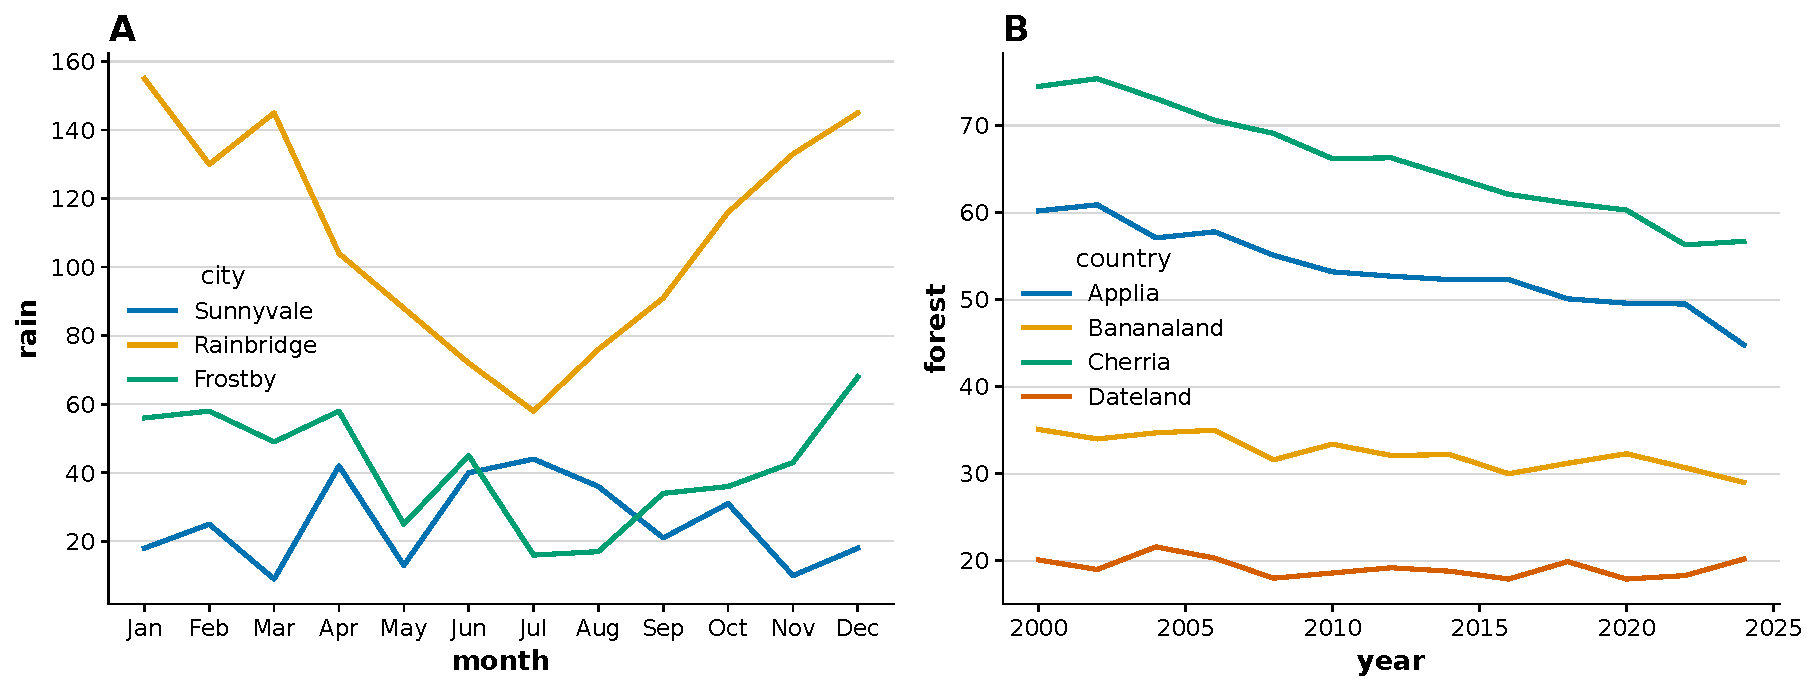
\includegraphics[width=0.72\textwidth,height=0.36\textheight,keepaspectratio]{figures/lesson07_example4_lesson7_two_tables.pdf}
\captionof{figure}{Lesson 7, example 4: \code{lesson7\_\allowbreak{}two\_\allowbreak{}tables.\allowbreak{}png}.}
\end{minipage}\end{center}
\section*{Example 5}
\code{sdata.\allowbreak{}draw\_\allowbreak{}all\_\allowbreak{}pairs} draws every number column against every other, in one go.
\begin{lstlisting}[style=py]
import simplydata as sdata
pairs = sdata.draw_all_pairs(sdata.get_example("marks"), colour="class")
pairs.save("lesson7_pairs.png")
\end{lstlisting}
\whateachline
\begin{lineexplain}
  \item[1] Load simplydata.
  \item[2] Hours, marks and height, each against each other. The middle line shows how each column is spread out.
  \item[3] Save it. Which two columns go together?
\end{lineexplain}
\printedoutput{output/lesson07_example5.txt}
\begin{center}\begin{minipage}{\linewidth}\centering
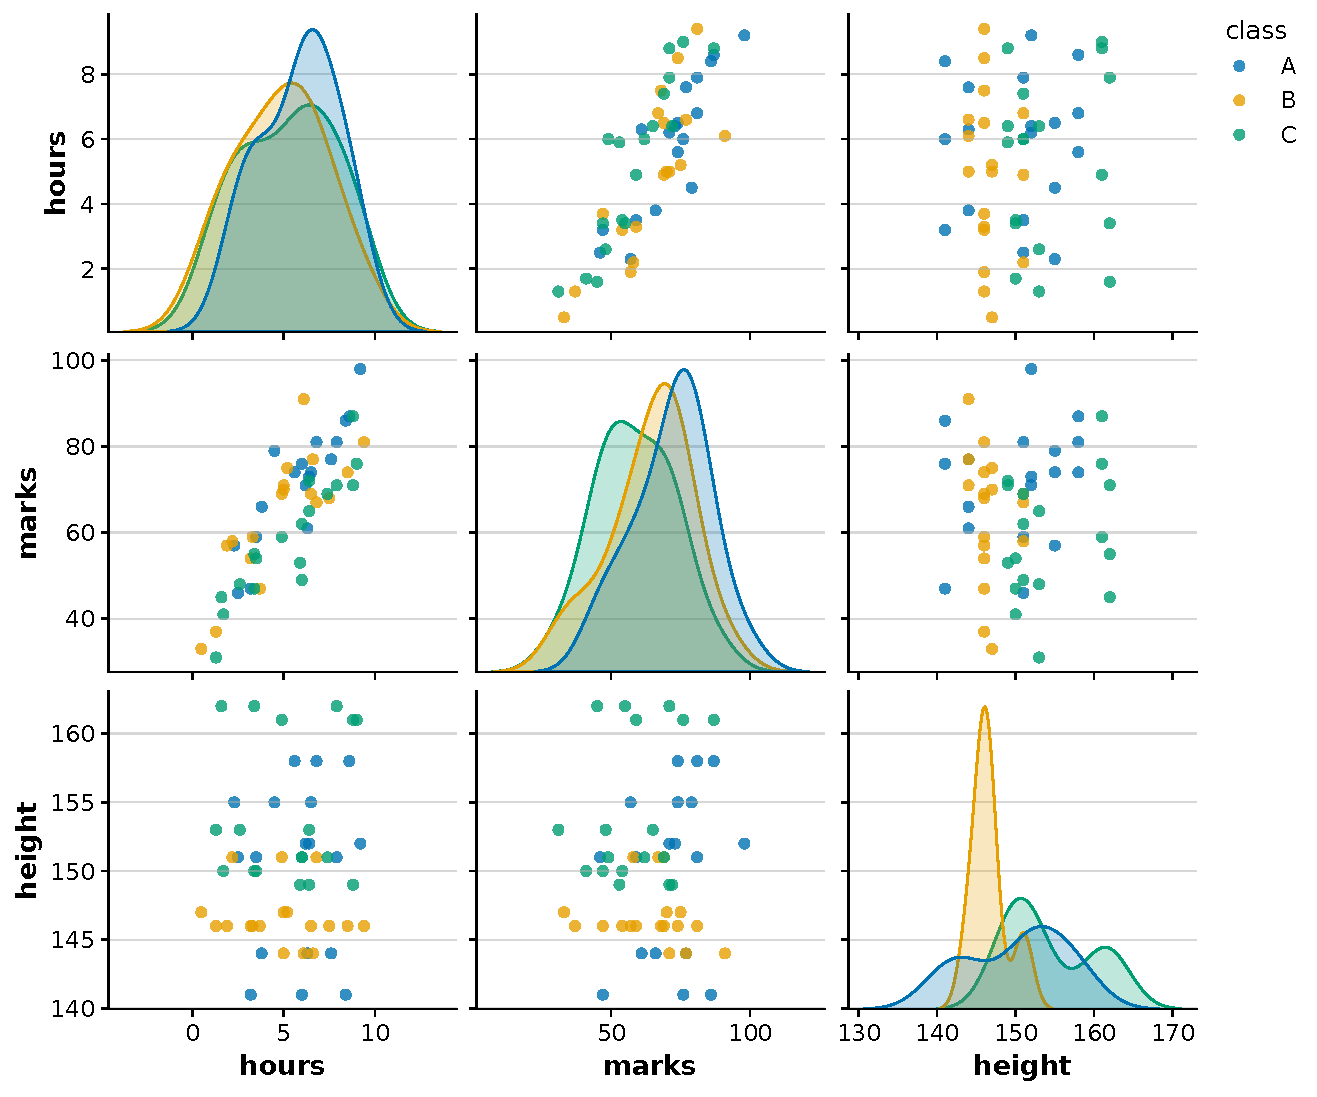
\includegraphics[width=0.72\textwidth,height=0.36\textheight,keepaspectratio]{figures/lesson07_example5_lesson7_pairs.pdf}
\captionof{figure}{Lesson 7, example 5: \code{lesson7\_\allowbreak{}pairs.\allowbreak{}png}.}
\end{minipage}\end{center}
\begin{goodtoknow}
\begin{itemize}
  \item \code{same\_\allowbreak{}y=True} gives all the charts on a page the same y-axis, so heights can be compared fairly: \code{sdata.\allowbreak{}put\_\allowbreak{}side\_\allowbreak{}by\_\allowbreak{}side(a,\allowbreak{} b,\allowbreak{} same\_\allowbreak{}y=True)}.
  \item \code{sdata.\allowbreak{}put\_\allowbreak{}side\_\allowbreak{}by\_\allowbreak{}side}, \code{sdata.\allowbreak{}put\_\allowbreak{}one\_\allowbreak{}above\_\allowbreak{}other} and \code{sdata.\allowbreak{}put\_\allowbreak{}in\_\allowbreak{}rows\_\allowbreak{}and\_\allowbreak{}columns} all take \code{with\_\allowbreak{}letters=True}.
  \item \code{chart.\allowbreak{}draw\_\allowbreak{}one\_\allowbreak{}chart\_\allowbreak{}for\_\allowbreak{}each\_\allowbreak{}group\_\allowbreak{}in(down=\textquotedbl{}class\textquotedbl{},\allowbreak{} across=\textquotedbl{}subject\textquotedbl{})} makes a table of small charts: the classes go down, the subjects go across. \code{per\_\allowbreak{}row=3} puts 3 small charts in a row.
\end{itemize}
\end{goodtoknow}
\begin{tryit}
\begin{enumerate}
  \item Change \code{chart.\allowbreak{}draw\_\allowbreak{}one\_\allowbreak{}chart\_\allowbreak{}for\_\allowbreak{}each\_\allowbreak{}group\_\allowbreak{}in(\textquotedbl{}class\textquotedbl{})} to \code{chart.\allowbreak{}draw\_\allowbreak{}one\_\allowbreak{}chart\_\allowbreak{}for\_\allowbreak{}each\_\allowbreak{}group\_\allowbreak{}in(\textquotedbl{}subject\textquotedbl{})}.
  \item Use \code{sdata.\allowbreak{}put\_\allowbreak{}side\_\allowbreak{}by\_\allowbreak{}side(a,\allowbreak{} b)} instead of \code{sdata.\allowbreak{}put\_\allowbreak{}one\_\allowbreak{}above\_\allowbreak{}other(a,\allowbreak{} b)} for the weather charts.
  \item Make \code{sdata.\allowbreak{}draw\_\allowbreak{}all\_\allowbreak{}pairs} of \code{sdata.\allowbreak{}get\_\allowbreak{}example(\textquotedbl{}weather\textquotedbl{})} with \code{colour=\textquotedbl{}city\textquotedbl{}}.
\end{enumerate}
Worked solutions: page~\pageref{solutions:7}, or type \code{sdata.\allowbreak{}show\_\allowbreak{}lesson(7,\allowbreak{} solutions=True)}.
\end{tryit}
\par\noindent{\small\sffamily\textbf{Words in this lesson:} \hyperref[word:draw-one-chart-for-each-group-in]{\code{chart.\allowbreak{}draw\_\allowbreak{}one\_\allowbreak{}chart\_\allowbreak{}for\_\allowbreak{}each\_\allowbreak{}group\_\allowbreak{}in()}}, \hyperref[word:sdata.put-one-above-other]{\code{sdata.\allowbreak{}put\_\allowbreak{}one\_\allowbreak{}above\_\allowbreak{}other()}}, \hyperref[word:sdata.put-in-rows-and-columns]{\code{sdata.\allowbreak{}put\_\allowbreak{}in\_\allowbreak{}rows\_\allowbreak{}and\_\allowbreak{}columns()}}, \hyperref[word:sdata.put-side-by-side]{\code{sdata.\allowbreak{}put\_\allowbreak{}side\_\allowbreak{}by\_\allowbreak{}side()}}, \hyperref[word:sdata.draw-all-pairs]{\code{sdata.\allowbreak{}draw\_\allowbreak{}all\_\allowbreak{}pairs()}}, \hyperref[word:fit-line]{\code{chart.\allowbreak{}fit\_\allowbreak{}line()}}, \hyperref[word:draw-histogram]{\code{chart.\allowbreak{}draw\_\allowbreak{}histogram()}}.\par}

\chapter{Hard tricks, and your own program}\label{lesson:8}
\begin{learnbox}
\begin{itemize}
  \item a second y-axis, a zoom box and a moving chart
  \item a heatmap that sorts itself
  \item how to write your own program from start to end
\end{itemize}
\end{learnbox}
\section*{Example 1}
A second y-axis shows a column measured in other units on the same chart.
\begin{lstlisting}[style=py]
import simplydata as sdata
weather = sdata.get_example("weather")
chart = sdata.chart(weather)
chart.draw_lines(x="month", y="temperature")
chart.add_second_y("rain", drawn_as="bars", labelled="Rain (mm)")
chart.label_y("Temperature (°C)")
chart.save("lesson8_second_y.png")
\end{lstlisting}
\whateachline
\begin{lineexplain}
  \item[1] Load simplydata.
  \item[2] Get the weather table.
  \item[3] Start a chart.
  \item[4] A line of temperature (average of the three cities).
  \item[5] Add rain, drawn as bars, with its own y-axis on the right.
  \item[6] Name the left y-axis.
  \item[7] Save it.
\end{lineexplain}
\printedoutput{output/lesson08_example1.txt}
\begin{center}\begin{minipage}{\linewidth}\centering
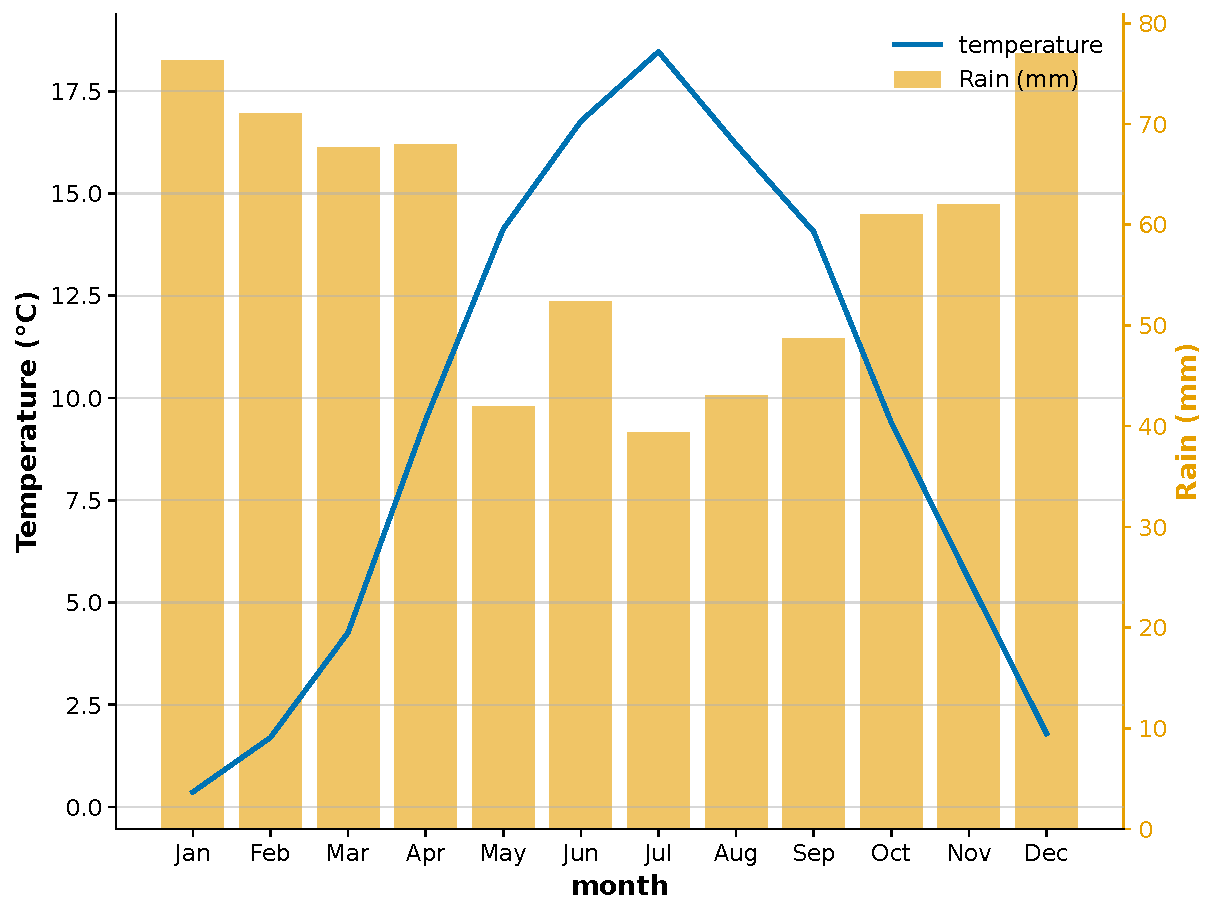
\includegraphics[width=0.72\textwidth,height=0.36\textheight,keepaspectratio]{figures/lesson08_example1_lesson8_second_y.pdf}
\captionof{figure}{Lesson 8, example 1: \code{lesson8\_\allowbreak{}second\_\allowbreak{}y.\allowbreak{}png}.}
\end{minipage}\end{center}
\section*{Example 2}
A zoom box shows a small part of the chart close up.
\begin{lstlisting}[style=py]
import simplydata as sdata
marks = sdata.get_example("marks")
chart = sdata.chart(marks)
chart.draw_dots(x="hours", y="marks")
chart.add_zoom_box(x_between=[2, 4], y_between=[40, 60], where="top left")
chart.save("lesson8_zoom.png")
\end{lstlisting}
\whateachline
\begin{lineexplain}
  \item[1] Load simplydata.
  \item[2] Get the marks table.
  \item[3] Start a chart.
  \item[4] Dots of hours and marks.
  \item[5] Show the part between 2 and 4 hours and between 40 and 60 marks, bigger, in a box at the top left.
  \item[6] Save it.
\end{lineexplain}
\printedoutput{output/lesson08_example2.txt}
\begin{center}\begin{minipage}{\linewidth}\centering
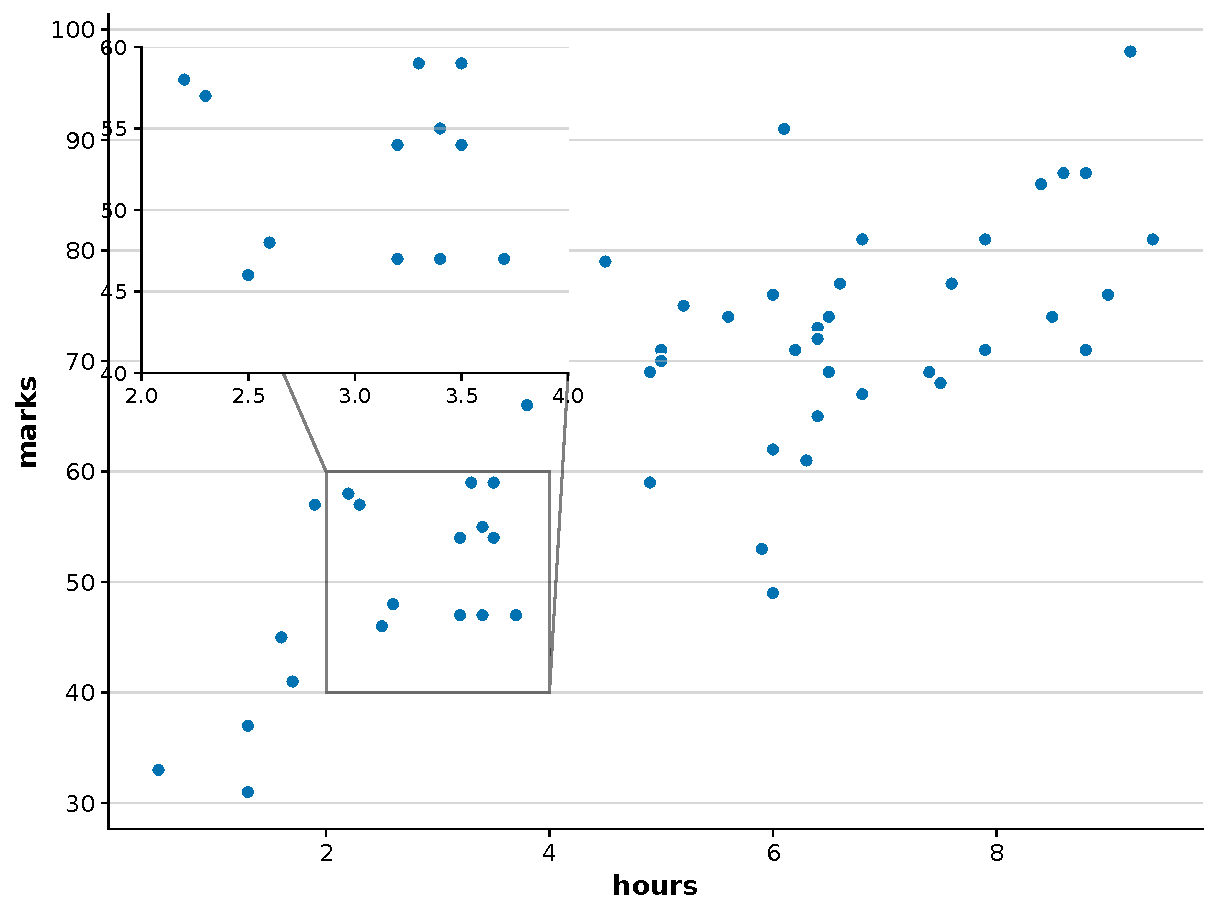
\includegraphics[width=0.72\textwidth,height=0.36\textheight,keepaspectratio]{figures/lesson08_example2_lesson8_zoom.pdf}
\captionof{figure}{Lesson 8, example 2: \code{lesson8\_\allowbreak{}zoom.\allowbreak{}png}.}
\end{minipage}\end{center}
\section*{Example 3}
A heatmap colours a grid of numbers. \code{cluster=True} puts rows that are alike next to each other.
\begin{lstlisting}[style=py]
import simplydata as sdata
weather = sdata.get_example("weather")
chart = sdata.chart(weather)
chart.draw_heatmap(x="month", y="city", value="rain", with_numbers=True, cluster=True)
chart.label_colour_bar("Rain (mm)")
chart.set_size(width=12, height=4)
chart.save("lesson8_heatmap.png")
\end{lstlisting}
\whateachline
\begin{lineexplain}
  \item[1] Load simplydata.
  \item[2] Get the weather table.
  \item[3] Start a chart.
  \item[4] One square per city and month, coloured by rain, with the number written in. \code{cluster=True} sorts the rows and columns and draws a tree of how alike they are (hierarchical clustering).
  \item[5] Name the colour bar.
  \item[6] Make the chart wide and low.
  \item[7] Save it.
\end{lineexplain}
\printedoutput{output/lesson08_example3.txt}
\begin{center}\begin{minipage}{\linewidth}\centering
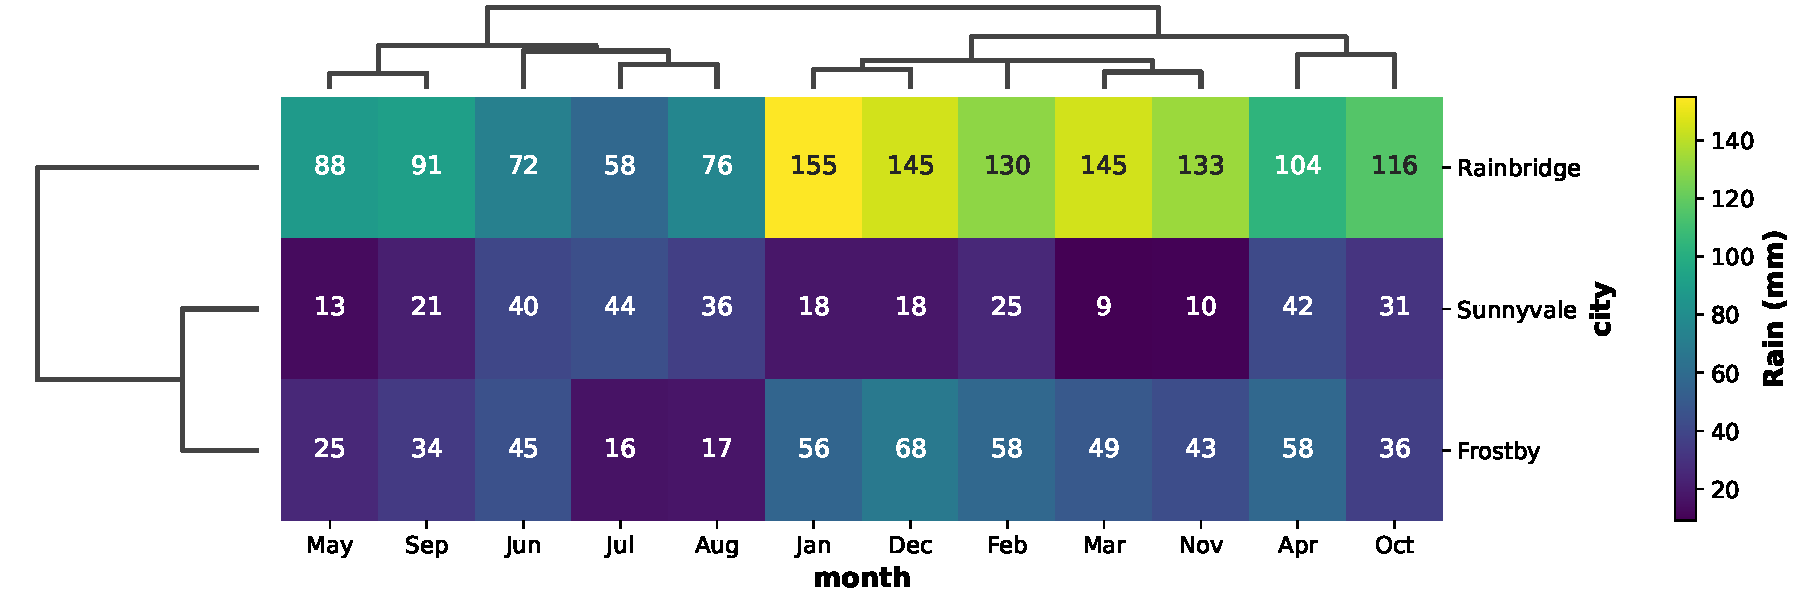
\includegraphics[width=0.72\textwidth,height=0.36\textheight,keepaspectratio]{figures/lesson08_example3_lesson8_heatmap.pdf}
\captionof{figure}{Lesson 8, example 3: \code{lesson8\_\allowbreak{}heatmap.\allowbreak{}png}.}
\end{minipage}\end{center}
\section*{Example 4}
An animation is a chart that moves: one picture for each value of a column.
\begin{lstlisting}[style=py]
import simplydata as sdata
growth = sdata.get_example("growth")
chart = sdata.chart(growth)
chart.draw_bars(x="country", y="population")
chart.set_range_y(0, 50)
chart.animate(over="year")
chart.save("lesson8_growth.gif")
\end{lstlisting}
\whateachline
\begin{lineexplain}
  \item[1] Load simplydata.
  \item[2] Get the growth table.
  \item[3] Start a chart.
  \item[4] One bar per country.
  \item[5] Keep the y-axis still, from 0 to 50.
  \item[6] Make one picture for each year.
  \item[7] Save it as a \code{.\allowbreak{}gif}, a moving picture. Open it in a web browser to watch.
\end{lineexplain}
\printedoutput{output/lesson08_example4.txt}
\begin{center}\begin{minipage}{\linewidth}\centering
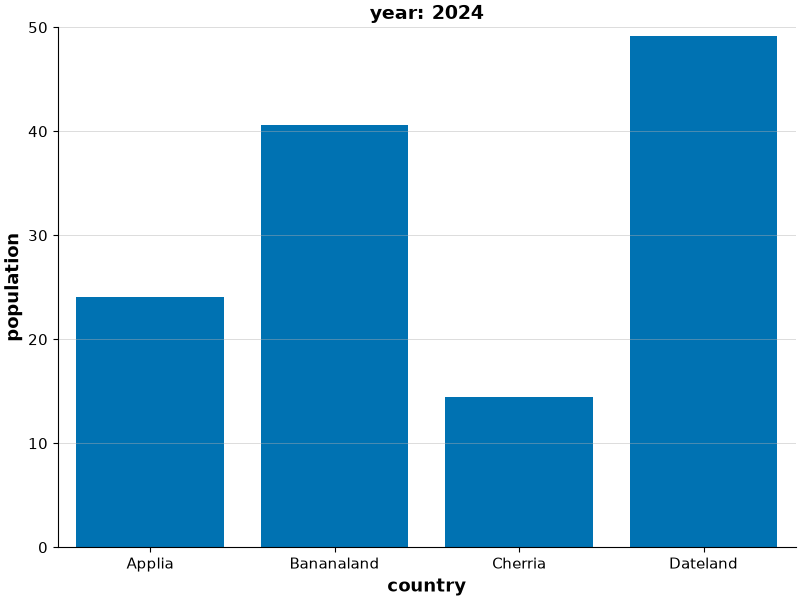
\includegraphics[width=0.72\textwidth,height=0.36\textheight,keepaspectratio]{figures/lesson08_example4_lesson8_growth.png}
\captionof{figure}{Lesson 8, example 4: \code{lesson8\_\allowbreak{}growth.\allowbreak{}gif} (the last picture of the animation).}
\end{minipage}\end{center}
\section*{Example 5}
Your own program. Every chart follows the same plan: get the data, look, start, draw, words, look, save.
\begin{lstlisting}[style=py]
import simplydata as sdata
island = sdata.get_example("island")
print(island)
chart = sdata.chart(island)
chart.draw_contour(x="east", y="north", z="height")
chart.write_title_on_top("Treasure Island")
chart.label_x("East (km)")
chart.label_y("North (km)")
chart.label_colour_bar("Height (m)")
chart.write_note("X marks the spot", x=10, y=4, with_arrow=True)
chart.use_style("presentation")
chart.save("lesson8_my_program.png")
\end{lstlisting}
\whateachline
\begin{lineexplain}
  \item[1] 1. Load simplydata.
  \item[2] 2. Get the data. For your own file, skip this line and write chart = \code{sdata.\allowbreak{}chart(\textquotedbl{}my\_\allowbreak{}file.\allowbreak{}xlsx\textquotedbl{})} below.
  \item[3] 3. Look at the data before you draw it.
  \item[4] 4. Start a chart.
  \item[5] 5. Draw: a map where each colour band is one height.
  \item[6] 6. Words: a title ...
  \item[7] ... and the axis names ...
  \item[9] ... and the name of the colour bar.
  \item[10] A note with an arrow.
  \item[11] 7. Look: big and clear for showing to others.
  \item[12] 8. Save.
\end{lineexplain}
\printedoutput{output/lesson08_example5.txt}
\begin{center}\begin{minipage}{\linewidth}\centering
\includegraphics[width=0.72\textwidth,height=0.36\textheight,keepaspectratio]{figures/lesson08_example5_lesson8_my_program.pdf}
\captionof{figure}{Lesson 8, example 5: \code{lesson8\_\allowbreak{}my\_\allowbreak{}program.\allowbreak{}png}.}
\end{minipage}\end{center}
\begin{goodtoknow}
\begin{itemize}
  \item Those are all the charts! \code{sdata.\allowbreak{}show\_\allowbreak{}all\_\allowbreak{}words()} lists every word and \code{sdata.\allowbreak{}help(\textquotedbl{}word\textquotedbl{})} explains any of them. Lessons 9 to 12 teach tables: how to look at your data, clean it and sum it up before you draw it.
  \item Your own data: save it from Excel as \code{.\allowbreak{}xlsx} or \code{.\allowbreak{}csv}, then chart = \code{sdata.\allowbreak{}chart(\textquotedbl{}my\_\allowbreak{}file.\allowbreak{}xlsx\textquotedbl{})}. If a column name is spelt wrong, simplydata tells you the right one.
\end{itemize}
\end{goodtoknow}
\begin{tryit}
\begin{enumerate}
  \item Write your own program, from an empty file, for a question you care about.
  \item Use any example table, or your own. Give it a title, axis names and a note.
  \item Make a second chart of the same table, put the two charts side by side and save the page as a PDF.
\end{enumerate}
Worked solutions: page~\pageref{solutions:8}, or type \code{sdata.\allowbreak{}show\_\allowbreak{}lesson(8,\allowbreak{} solutions=True)}.
\end{tryit}
\par\noindent{\small\sffamily\textbf{Words in this lesson:} \hyperref[word:add-second-y]{\code{chart.\allowbreak{}add\_\allowbreak{}second\_\allowbreak{}y()}}, \hyperref[word:add-zoom-box]{\code{chart.\allowbreak{}add\_\allowbreak{}zoom\_\allowbreak{}box()}}, \hyperref[word:draw-heatmap]{\code{chart.\allowbreak{}draw\_\allowbreak{}heatmap()}}, \hyperref[word:label-colour-bar]{\code{chart.\allowbreak{}label\_\allowbreak{}colour\_\allowbreak{}bar()}}, \hyperref[word:set-size]{\code{chart.\allowbreak{}set\_\allowbreak{}size()}}, \hyperref[word:animate]{\code{chart.\allowbreak{}animate()}}, \hyperref[word:draw-contour]{\code{chart.\allowbreak{}draw\_\allowbreak{}contour()}}, \hyperref[word:write-note]{\code{chart.\allowbreak{}write\_\allowbreak{}note()}}, \hyperref[word:use-style]{\code{chart.\allowbreak{}use\_\allowbreak{}style()}}, \hyperref[word:sdata.show-all-words]{\code{sdata.\allowbreak{}show\_\allowbreak{}all\_\allowbreak{}words()}}, \hyperref[word:sdata.help]{\code{sdata.\allowbreak{}help()}}.\par}

\chapter{Tables: open one and look at it}\label{lesson:9}
\begin{learnbox}
\begin{itemize}
  \item how to turn data into a simplydata table
  \item how to look at the first and last rows, and the names of the columns
  \item how to describe every column and count what is in it
\end{itemize}
\end{learnbox}
\section*{Example 1}
Before you draw, look at your data. \code{sdata.\allowbreak{}table} gives you plain words for that.
\begin{lstlisting}[style=py]
import simplydata as sdata
table = sdata.table(sdata.get_example("marks"))
print(table)
table.show_first_rows(5)
table.show_last_rows(3)
print(table.get_column_names())
table.describe_columns()
table.count_rows()
\end{lstlisting}
\whateachline
\begin{lineexplain}
  \item[1] Load simplydata.
  \item[2] Make a table from the practice marks. For your own file, write \code{sdata.\allowbreak{}table(\textquotedbl{}my\_\allowbreak{}file.\allowbreak{}xlsx\textquotedbl{})}.
  \item[3] Print the table. The first line says how many rows and columns it has. Then come the first 10 rows.
  \item[4] Show only the first 5 rows.
  \item[5] Show the last 3 rows.
  \item[6] Print the names of the columns.
  \item[7] Describe every column: is it numbers or text, how many cells are empty, and the smallest, biggest and average number.
  \item[8] Count the rows, and say the answer in a sentence. One row is one child in one test.
\end{lineexplain}
\printedoutput{output/lesson09_example1.txt}
\section*{Example 2}
\code{count\_\allowbreak{}each} counts how often each different value comes up.
\begin{lstlisting}[style=py]
import simplydata as sdata
table = sdata.table(sdata.get_example("fruit"))
table.show_first_rows()
table.count_each("fruit")
table.count_each("shop")
\end{lstlisting}
\whateachline
\begin{lineexplain}
  \item[1] Load simplydata.
  \item[2] Make a table of fruit sold by two shops.
  \item[3] Show the first rows. With nothing in the brackets you get 5.
  \item[4] For each fruit: in how many rows it comes up. It says the answer in a sentence, and gives back a small table that also has the percent of all the rows.
  \item[5] The same for each shop.
\end{lineexplain}
\printedoutput{output/lesson09_example2.txt}
\section*{Example 3}
\code{sdata.\allowbreak{}table} can read many files at once. Here we first save two small files, then read them back together.
\begin{lstlisting}[style=py]
import simplydata as sdata
weather = sdata.table(sdata.get_example("weather"))
weather.keep_first_rows(12)
weather.save("lesson9_part1.csv")
weather.start_again()
weather.keep_last_rows(12)
weather.save("lesson9_part2.csv")
both = sdata.table("lesson9_part*.csv")
both.count_each("file")
both.show(rows=3)
\end{lstlisting}
\whateachline
\begin{lineexplain}
  \item[1] Load simplydata.
  \item[2] Make a table of the weather.
  \item[3] Keep the first 12 rows: one city, a whole year.
  \item[4] Save them as a CSV file.
  \item[5] Back to the whole table.
  \item[6] Keep the last 12 rows: another city.
  \item[7] Save them as a second file.
  \item[8] Read every file whose name fits the pattern (* stands for any text) and stack them. A new column, \code{\textquotedbl{}file\textquotedbl{}}, says where each row came from.
  \item[9] 12 rows from each file.
  \item[10] Show the first 3 rows with every column. \code{both.\allowbreak{}show()} shows the whole table.
\end{lineexplain}
\printedoutput{output/lesson09_example3.txt}
\begin{goodtoknow}
\begin{itemize}
  \item Looking never changes the table. Only steps that say what they change (\code{keep\_\allowbreak{}rows\_\allowbreak{}where}, \code{sort\_\allowbreak{}by} ...) do, and lesson 10 shows them.
  \item In Jupyter, VS Code or Spyder, write table on the last line of a cell to see it as a nice table.
  \item \code{sdata.\allowbreak{}table} reads the same files as \code{sdata.\allowbreak{}chart}: \code{.\allowbreak{}xlsx}, \code{.\allowbreak{}csv}, \code{.\allowbreak{}tsv}, \code{.\allowbreak{}parquet} and \code{.\allowbreak{}json}. For one sheet of an Excel file: \code{sdata.\allowbreak{}table(\textquotedbl{}results.\allowbreak{}xlsx\textquotedbl{},\allowbreak{} sheet=\textquotedbl{}2026\textquotedbl{})}.
  \item The row numbers on the left start at 1, the way people count: the last row of a table of 54 rows is row 54. Lesson 10 uses these numbers to choose rows by their place.
  \item A folder works too: \code{sdata.\allowbreak{}table(\textquotedbl{}data/\textquotedbl{})} reads every table file in it. A web address works like a file name: \code{sdata.\allowbreak{}table(\textquotedbl{}https://example.\allowbreak{}org/data.\allowbreak{}csv\textquotedbl{})}.
  \item Files written in another way: \code{separator=\textquotedbl{};\textquotedbl{}}, \code{decimal\_\allowbreak{}mark=\textquotedbl{},\allowbreak{}\textquotedbl{}} (3,5 is three and a half), \code{thousands\_\allowbreak{}mark=\textquotedbl{}.\allowbreak{}\textquotedbl{}}, \code{empty\_\allowbreak{}values=[\textquotedbl{}NA\textquotedbl{},\allowbreak{} \textquotedbl{}-\textquotedbl{}]}, \code{skip\_\allowbreak{}rows=2} and \code{encoding=\textquotedbl{}latin-1\textquotedbl{}}.
\end{itemize}
\end{goodtoknow}
\begin{tryit}
\begin{enumerate}
  \item Make a table of \code{sdata.\allowbreak{}get\_\allowbreak{}example(\textquotedbl{}weather\textquotedbl{})}. How many rows does it have?
  \item Describe its columns. Which column has the biggest numbers?
  \item Count each \code{\textquotedbl{}city\textquotedbl{}}. Does every city have the same number of rows?
\end{enumerate}
Worked solutions: page~\pageref{solutions:9}, or type \code{sdata.\allowbreak{}show\_\allowbreak{}lesson(9,\allowbreak{} solutions=True)}.
\end{tryit}
\par\noindent{\small\sffamily\textbf{Words in this lesson:} \hyperref[word:sdata.table]{\code{sdata.\allowbreak{}table()}}, \hyperref[word:table.show-first-rows]{\code{table.\allowbreak{}show\_\allowbreak{}first\_\allowbreak{}rows()}}, \hyperref[word:table.show-last-rows]{\code{table.\allowbreak{}show\_\allowbreak{}last\_\allowbreak{}rows()}}, \hyperref[word:table.get-column-names]{\code{table.\allowbreak{}get\_\allowbreak{}column\_\allowbreak{}names()}}, \hyperref[word:table.describe-columns]{\code{table.\allowbreak{}describe\_\allowbreak{}columns()}}, \hyperref[word:table.count-rows]{\code{table.\allowbreak{}count\_\allowbreak{}rows()}}, \hyperref[word:table.count-each]{\code{table.\allowbreak{}count\_\allowbreak{}each()}}, \hyperref[word:table.show]{\code{table.\allowbreak{}show()}}.\par}

\chapter{Tables: choose rows and columns, and undo}\label{lesson:10}
\begin{learnbox}
\begin{itemize}
  \item how to keep only the columns and rows you want
  \item how to sort the rows
  \item how to take a step back, and start again
  \item how to save your table
\end{itemize}
\end{learnbox}
\section*{Example 1}
A table is changed in small steps, like a chart. Each step says what it did.
\begin{lstlisting}[style=py]
import simplydata as sdata
table = sdata.table(sdata.get_example("marks"))
table.keep_columns("name", "subject", "marks")
table.keep_rows_where("subject", is_equal_to="Maths")
table.keep_rows_where("marks", is_above=60)
table.sort_by("marks", biggest_first=True)
table.show_first_rows(10)
table.show_steps()
table.undo()
table.start_again()
print(table)
\end{lstlisting}
\whateachline
\begin{lineexplain}
  \item[1] Load simplydata.
  \item[2] Make a table of the marks.
  \item[3] Keep only these three columns, in this order.
  \item[4] Keep only the rows where the subject is Maths. simplydata says how many rows it kept.
  \item[5] Of those, keep only marks above 60.
  \item[6] Put the rows in order, the biggest mark first.
  \item[7] Show the first 10 rows: the best Maths marks.
  \item[8] List every step you did, in order.
  \item[9] Take back the last step (the sorting).
  \item[10] Go back to the whole table, as it was at the start.
  \item[11] All 54 rows and 6 columns are back.
\end{lineexplain}
\printedoutput{output/lesson10_example1.txt}
\section*{Example 2}
\code{keep\_\allowbreak{}rows\_\allowbreak{}where} and \code{remove\_\allowbreak{}rows\_\allowbreak{}where} know many conditions. Then save what you made.
\begin{lstlisting}[style=py]
import simplydata as sdata
table = sdata.table(sdata.get_example("weather"))
table.keep_rows_where("month_number", is_between=[6, 8])
table.remove_rows_where("city", is_equal_to="Frostby")
table.remove_columns("wind_direction", "wind_speed")
table.rename_column("temperature", to="temp")
print(table)
table.save("lesson10_summer.xlsx")
\end{lstlisting}
\whateachline
\begin{lineexplain}
  \item[1] Load simplydata.
  \item[2] Make a table of the weather.
  \item[3] Keep the summer months: 6, 7 and 8. \code{is\_\allowbreak{}between=} keeps both ends.
  \item[4] Remove the rows of the city Frostby.
  \item[5] Remove two columns we do not need.
  \item[6] Give the column \code{\textquotedbl{}temperature\textquotedbl{}} the shorter name \code{\textquotedbl{}temp\textquotedbl{}}.
  \item[7] Look at what is left: 6 rows and 5 columns.
  \item[8] Save the table as an Excel file. A name ending in \code{.\allowbreak{}csv} saves a CSV file.
\end{lineexplain}
\printedoutput{output/lesson10_example2.txt}
\section*{Example 3}
A condition can also be written out, with and, or, not and brackets. And \code{keep\_\allowbreak{}biggest\_\allowbreak{}rows} keeps the top rows of each group.
\begin{lstlisting}[style=py]
import simplydata as sdata
table = sdata.table(sdata.get_example("marks"))
table.keep_rows_where("marks > 60 and subject == 'Maths'")
table.undo()
table.remove_rows_where("hours < 3 or class in ['B', 'C']")
table.start_again()
table.keep_biggest_rows(2, by="marks", for_each_group_in="subject")
table.show()
\end{lstlisting}
\whateachline
\begin{lineexplain}
  \item[1] Load simplydata.
  \item[2] Make a table of the marks.
  \item[3] Keep the rows where both are true: a mark above 60, in Maths. Text goes in quotes, and == means \code{\textquotedbl{}is equal to\textquotedbl{}}.
  \item[4] Back to all the rows.
  \item[5] Remove the rows where at least one is true: under 3 hours of study, or class B or C.
  \item[6] Back to the whole table.
  \item[7] Keep the 2 best marks in each subject: 6 rows.
  \item[8] Show the whole (small) table.
\end{lineexplain}
\printedoutput{output/lesson10_example3.txt}
\section*{Example 4}
Rows and columns can also be chosen by their place in the table. Positions count from 1, the numbers \code{table.\allowbreak{}show()} prints, and both ends are included.
\begin{lstlisting}[style=py]
import simplydata as sdata
table = sdata.table(sdata.get_example("marks"))
table.show_last_rows(3)
table.keep_rows_by_position(10, to=20)
table.keep_rows_by_position(1, step=2)
table.keep_columns_by_position(1, to=3)
table.show()
table.start_again()
print(table.get_cell_at(row=3, column="marks"))
table.reverse_rows()
table.show_first_rows(3)
\end{lstlisting}
\whateachline
\begin{lineexplain}
  \item[1] Load simplydata.
  \item[2] Make a table of the marks.
  \item[3] The last three rows are numbered 52, 53 and 54: rows count from 1.
  \item[4] Keep rows 10 to 20. Both ends are included, so that is 11 rows.
  \item[5] Of those, keep every 2nd row: the 1st, 3rd, 5th ... 6 rows.
  \item[6] Keep the first three columns. It says which columns they were.
  \item[7] 6 rows and 3 columns, numbered again from 1.
  \item[8] Back to the whole table.
  \item[9] One cell: the mark in row 3. \code{get\_\allowbreak{}cell\_\allowbreak{}at} only looks; the table does not change.
  \item[10] Turn the table upside down: the last row comes first.
  \item[11] Rosa's marks are on top now.
\end{lineexplain}
\printedoutput{output/lesson10_example4.txt}
\begin{goodtoknow}
\begin{itemize}
  \item Conditions for \code{keep\_\allowbreak{}rows\_\allowbreak{}where} and \code{remove\_\allowbreak{}rows\_\allowbreak{}where}: \code{is\_\allowbreak{}above}, \code{is\_\allowbreak{}below}, \code{is\_\allowbreak{}at\_\allowbreak{}least}, \code{is\_\allowbreak{}at\_\allowbreak{}most}, \code{is\_\allowbreak{}equal\_\allowbreak{}to}, \code{is\_\allowbreak{}not\_\allowbreak{}equal\_\allowbreak{}to}, \code{is\_\allowbreak{}between}, \code{is\_\allowbreak{}one\_\allowbreak{}of}, contains, \code{starts\_\allowbreak{}with}, \code{ends\_\allowbreak{}with} and \code{is\_\allowbreak{}empty}.
  \item \code{is\_\allowbreak{}one\_\allowbreak{}of=} takes a list: \code{table.\allowbreak{}keep\_\allowbreak{}rows\_\allowbreak{}where(\textquotedbl{}subject\textquotedbl{},\allowbreak{} is\_\allowbreak{}one\_\allowbreak{}of=[\textquotedbl{}Maths\textquotedbl{},\allowbreak{} \textquotedbl{}Science\textquotedbl{}])}.
  \item \code{undo()} takes back one step at a time. \code{start\_\allowbreak{}again()} is a step too, so \code{undo()} can take it back.
  \item Your file is never changed: only \code{table.\allowbreak{}save(.\allowbreak{}.\allowbreak{}.\allowbreak{})} writes a file.
  \item Written conditions use == != \textless{} \textless{}= \textgreater{} \textgreater{}=, and, or, not, brackets, in [...] and is empty. An empty cell never meets a condition, and not does not change that: \code{\textquotedbl{}not (marks \textgreater{} 50)\textquotedbl{}} leaves out empty marks too. To find them, write \code{\textquotedbl{}marks is empty\textquotedbl{}}. A note says how many rows had an empty cell.
  \item Dates go in quotes as year-month-day: \code{table.\allowbreak{}keep\_\allowbreak{}rows\_\allowbreak{}where(\textquotedbl{}date \textgreater{} '2026-03-01'\textquotedbl{})}, or \code{table.\allowbreak{}keep\_\allowbreak{}rows\_\allowbreak{}where(\textquotedbl{}date\textquotedbl{},\allowbreak{} is\_\allowbreak{}after=\textquotedbl{}2026-03-01\textquotedbl{})}.
  \item \code{keep\_\allowbreak{}rows\_\allowbreak{}where} chooses rows by their values, \code{keep\_\allowbreak{}rows\_\allowbreak{}by\_\allowbreak{}position} by their place. Positions count from 1 and both ends are included, so rows 10 to 20 are 11 rows. \code{to=\textquotedbl{}last\textquotedbl{}} goes to the end, and a list such as [1, 5, 9] keeps those rows in that order.
  \item Coming from pandas or NumPy, which count from 0 and leave out the end: df.iloc[9:20] is \code{table.\allowbreak{}keep\_\allowbreak{}rows\_\allowbreak{}by\_\allowbreak{}position(10,\allowbreak{} to=20)}, df.iloc[::2] is \code{keep\_\allowbreak{}rows\_\allowbreak{}by\_\allowbreak{}position(1,\allowbreak{} step=2)}, df.iloc[[0, 4]] is \code{keep\_\allowbreak{}rows\_\allowbreak{}by\_\allowbreak{}position([1,\allowbreak{} 5])}, df.iloc[:, 0:3] is \code{keep\_\allowbreak{}columns\_\allowbreak{}by\_\allowbreak{}position(1,\allowbreak{} to=3)}, df.loc[:, \code{\textquotedbl{}hours\textquotedbl{}}:\code{\textquotedbl{}height\textquotedbl{}}] is \code{keep\_\allowbreak{}columns(\textquotedbl{}hours\textquotedbl{},\allowbreak{} to=\textquotedbl{}height\textquotedbl{})}, \code{df.\allowbreak{}select\_\allowbreak{}dtypes(\textquotedbl{}number\textquotedbl{})} is \code{keep\_\allowbreak{}columns(of\_\allowbreak{}kind=\textquotedbl{}number\textquotedbl{})}, df.at[2, \code{\textquotedbl{}marks\textquotedbl{}}] is \code{get\_\allowbreak{}cell\_\allowbreak{}at(row=3,\allowbreak{} column=\textquotedbl{}marks\textquotedbl{})} and df.iloc[::-1] is \code{reverse\_\allowbreak{}rows()}. For numbers, a[2:8] is \code{nums.\allowbreak{}keep\_\allowbreak{}numbers\_\allowbreak{}by\_\allowbreak{}position(3,\allowbreak{} to=8)}, and for a grid, g[1:5, 0:3] is \code{grid.\allowbreak{}keep\_\allowbreak{}rows\_\allowbreak{}by\_\allowbreak{}position(2,\allowbreak{} to=5)}.keep\_columns\_by\_position(1, \code{to=3}).
\end{itemize}
\end{goodtoknow}
\begin{tryit}
\begin{enumerate}
  \item In the marks table, keep only class \code{\textquotedbl{}B\textquotedbl{}} and sort by \code{\textquotedbl{}hours\textquotedbl{}}. Who studied the longest?
  \item Undo the sorting, then sort by name instead.
  \item Keep 5 random rows with \code{table.\allowbreak{}keep\_\allowbreak{}random\_\allowbreak{}rows(5,\allowbreak{} with\_\allowbreak{}seed=1)} and save them as \code{\textquotedbl{}five.\allowbreak{}csv\textquotedbl{}}.
  \item With one written condition, keep the rows with marks below 50 or hours above 8. How many rows are there?
  \item From memory, without looking back: start again, keep rows 5 to 9, then remove the last row. How many rows are left, and whose name is in row 1 now?
\end{enumerate}
Worked solutions: page~\pageref{solutions:10}, or type \code{sdata.\allowbreak{}show\_\allowbreak{}lesson(10,\allowbreak{} solutions=True)}.
\end{tryit}
\par\noindent{\small\sffamily\textbf{Words in this lesson:} \hyperref[word:table.keep-columns]{\code{table.\allowbreak{}keep\_\allowbreak{}columns()}}, \hyperref[word:table.keep-rows-where]{\code{table.\allowbreak{}keep\_\allowbreak{}rows\_\allowbreak{}where()}}, \hyperref[word:table.sort-by]{\code{table.\allowbreak{}sort\_\allowbreak{}by()}}, \hyperref[word:table.show-steps]{\code{table.\allowbreak{}show\_\allowbreak{}steps()}}, \hyperref[word:table.undo]{\code{table.\allowbreak{}undo()}}, \hyperref[word:table.start-again]{\code{table.\allowbreak{}start\_\allowbreak{}again()}}, \hyperref[word:table.remove-rows-where]{\code{table.\allowbreak{}remove\_\allowbreak{}rows\_\allowbreak{}where()}}, \hyperref[word:table.remove-columns]{\code{table.\allowbreak{}remove\_\allowbreak{}columns()}}, \hyperref[word:table.rename-column]{\code{table.\allowbreak{}rename\_\allowbreak{}column()}}, \hyperref[word:table.save]{\code{table.\allowbreak{}save()}}, \hyperref[word:table.keep-random-rows]{\code{table.\allowbreak{}keep\_\allowbreak{}random\_\allowbreak{}rows()}}, \hyperref[word:table.keep-biggest-rows]{\code{table.\allowbreak{}keep\_\allowbreak{}biggest\_\allowbreak{}rows()}}, \hyperref[word:table.keep-rows-by-position]{\code{table.\allowbreak{}keep\_\allowbreak{}rows\_\allowbreak{}by\_\allowbreak{}position()}}, \hyperref[word:table.remove-rows-by-position]{\code{table.\allowbreak{}remove\_\allowbreak{}rows\_\allowbreak{}by\_\allowbreak{}position()}}, \hyperref[word:table.keep-columns-by-position]{\code{table.\allowbreak{}keep\_\allowbreak{}columns\_\allowbreak{}by\_\allowbreak{}position()}}, \hyperref[word:table.get-cell-at]{\code{table.\allowbreak{}get\_\allowbreak{}cell\_\allowbreak{}at()}}, \hyperref[word:table.reverse-rows]{\code{table.\allowbreak{}reverse\_\allowbreak{}rows()}}.\par}

\chapter{Tables: clean the data and add new columns}\label{lesson:11}
\begin{learnbox}
\begin{itemize}
  \item how to find and fill empty cells
  \item how to fix columns: numbers written as text, extra spaces, wrong values
  \item how to add new columns, in plain words or like a sum in maths
  \item what long and wide tables are
\end{itemize}
\end{learnbox}
\section*{Example 1}
Real data often has empty cells. The practice tables have none, so we make some first.
\begin{lstlisting}[style=py]
import simplydata as sdata
table = sdata.table(sdata.get_example("marks"))
table.replace_values_in("marks", [61, 73], with_value=None)
table.count_empty_cells_in()
table.fill_empty_cells_in("marks", with_the="average")
table.undo()
table.remove_rows_with_empty_cells_in("marks")
print(table)
\end{lstlisting}
\whateachline
\begin{lineexplain}
  \item[1] Load simplydata.
  \item[2] Make a table of the marks.
  \item[3] Make every mark of 61 or 73 empty. \code{with\_\allowbreak{}value=None} means an empty cell.
  \item[4] Show how many empty cells each column has.
  \item[5] Fill the empty marks with the average of the other marks.
  \item[6] Changed your mind? Take it back: the cells are empty again.
  \item[7] This time remove the rows with an empty cell in marks.
  \item[8] Some rows fewer than at the start.
\end{lineexplain}
\printedoutput{output/lesson11_example1.txt}
\section*{Example 2}
Data typed by people is often untidy. These words fix whole columns at once.
\begin{lstlisting}[style=py]
import simplydata as sdata
table = sdata.table({"name": ["  Asha", "ben ", "Chen"], "height": ["144", "152", "unknown"]})
table.remove_extra_spaces_in("name")
table.replace_values_in("name", "ben", with_value="Ben")
table.turn_into_numbers("height")
table.describe_columns()
\end{lstlisting}
\whateachline
\begin{lineexplain}
  \item[1] Load simplydata.
  \item[2] Make a small table by hand: each column name, then its values in a list.
  \item[3] Take away the spaces before and after the names.
  \item[4] Write \code{\textquotedbl{}ben\textquotedbl{}} with a capital letter.
  \item[5] Turn the heights from text into numbers. \code{\textquotedbl{}unknown\textquotedbl{}} is not a number, so that cell becomes empty, and simplydata tells you.
  \item[6] Now height is a column of numbers.
\end{lineexplain}
\printedoutput{output/lesson11_example2.txt}
\section*{Example 3}
A new column can be worked out from other columns, in plain words.
\begin{lstlisting}[style=py]
import simplydata as sdata
table = sdata.table(sdata.get_example("marks"))
table.add_column("marks_per_hour", by_dividing=["marks", "hours"])
table.add_group_column("grade", from_column="marks", cut_at=[40, 60, 80], names=["D", "C", "B", "A"])
table.show_first_rows()
table.count_each("grade")
\end{lstlisting}
\whateachline
\begin{lineexplain}
  \item[1] Load simplydata.
  \item[2] Make a table of the marks.
  \item[3] A new column called \code{\textquotedbl{}marks\_\allowbreak{}per\_\allowbreak{}hour\textquotedbl{}}: the marks divided by the hours.
  \item[4] A grade for each mark: below 40 is D, 40 to 59 is C, 60 to 79 is B, 80 and more is A.
  \item[5] Look at the two new columns on the right.
  \item[6] How many of each grade?
\end{lineexplain}
\printedoutput{output/lesson11_example3.txt}
\section*{Example 4}
Or write the new column like a sum in maths. Here each subject first gets its own column: the table goes from long to wide.
\begin{lstlisting}[style=py]
import simplydata as sdata
table = sdata.table(sdata.get_example("marks"))
table.keep_columns("name", "class", "subject", "marks")
table.turn_rows_into_columns(names_from="subject", values_from="marks")
table.add_column("total", "Maths + Science + English")
table.add_column("average", "total / 3")
table.add_rank_column("place", from_column="total")
table.sort_by("place")
table.show_first_rows()
\end{lstlisting}
\whateachline
\begin{lineexplain}
  \item[1] Load simplydata.
  \item[2] Make a table of the marks.
  \item[3] Keep the columns we need.
  \item[4] Make one column for each subject: Maths, Science and English. Each child now has one row.
  \item[5] A new column \code{\textquotedbl{}total\textquotedbl{}}: the three marks added up.
  \item[6] The average of the three marks.
  \item[7] Each child's place: 1 for the biggest total.
  \item[8] Put the rows in order of place.
  \item[9] Who came first?
\end{lineexplain}
\printedoutput{output/lesson11_example4.txt}
\section*{Example 5}
The shop table has real dates and some empty cells: days when the till broke. Look where they are, then fill them.
\begin{lstlisting}[style=py]
import simplydata as sdata
table = sdata.table(sdata.get_example("shop"))
table.count_empty_cells_in()
look = table.start_chart()
look.draw_map_of_empty_cells()
look.save("lesson11_empty_cells.png")
table.add_is_empty_column("sales_was_empty", from_column="sales")
table.fill_empty_cells_in("sales", with_the="line between neighbours", sorted_by="date", for_each_group_in="shop")
table.add_column_with_part_of_date("weekday", from_column="date", part="weekday name")
table.add_rolling_column("sales_7_days", from_column="sales", window=7, for_each_group_in="shop", sorted_by="date")
table.show(rows=8)
\end{lstlisting}
\whateachline
\begin{lineexplain}
  \item[1] Load simplydata.
  \item[2] Daily sales of two shops, January to March 2026.
  \item[3] 10 empty sales and 5 empty customer counts.
  \item[4] A chart of the table, to see where the empty cells are.
  \item[5] One strip per column and one line per row: empty cells are coloured, and each column says how many it has.
  \item[6] Save it.
  \item[7] Before filling: a True/False column that remembers which sales were empty.
  \item[8] Fill each gap on the straight line between the day before and the day after, in date order, for each shop on its own. A gap at the very start or end has a neighbour on one side only, so it stays empty, and a note says so.
  \item[9] A new column with the weekday of each date.
  \item[10] The average of each day and the 6 days before it: a 7-day moving average, which smooths out the busy weekends.
  \item[11] Look at the first 8 rows.
\end{lineexplain}
\printedoutput{output/lesson11_example5.txt}
\begin{center}\begin{minipage}{\linewidth}\centering
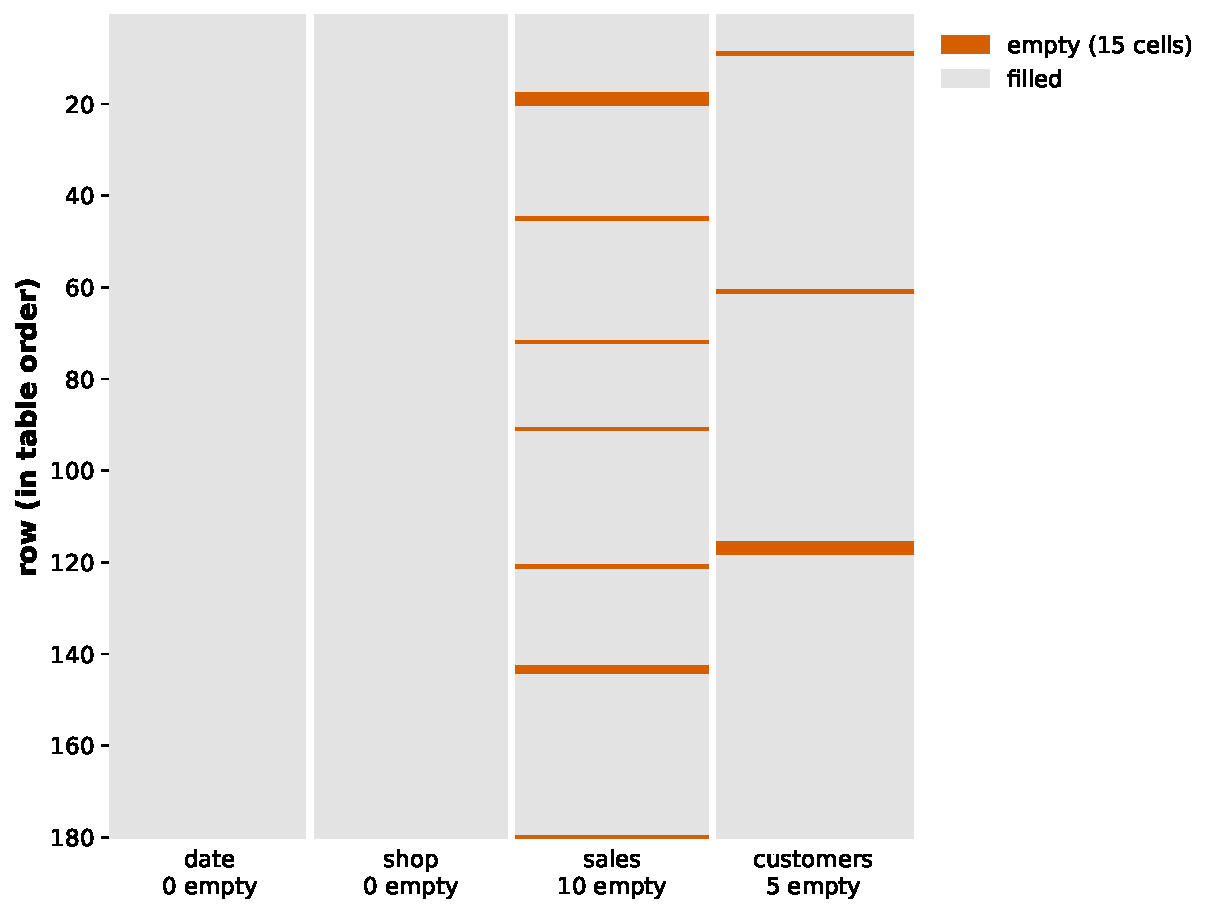
\includegraphics[width=0.72\textwidth,height=0.36\textheight,keepaspectratio]{figures/lesson11_example5_lesson11_empty_cells.pdf}
\captionof{figure}{Lesson 11, example 5: \code{lesson11\_\allowbreak{}empty\_\allowbreak{}cells.\allowbreak{}png}.}
\end{minipage}\end{center}
\section*{Example 6}
Names and dates typed in by people often need taking apart.
\begin{lstlisting}[style=py]
import simplydata as sdata
table = sdata.table({"name": ["Asha Rao", "Ben Lee", "Chen Wu"], "born": ["04/30/2014", "12/25/2013", "07/03/2014"], "height": [144.37, 152.81, 139.5]})
table.split_column("name", separator=" ", into=["first_name", "family_name"])
table.add_column_with_part_of_text("initial", from_column="first_name", first_characters=1)
table.replace_text_in("family_name", "Lee", with_value="Li")
table.turn_into_dates("born", order="month day year")
table.add_column_with_part_of_date("month_born", from_column="born", part="month name")
table.change_column("height", "height / 100")
table.round_numbers_in("height", 2)
table.show()
\end{lstlisting}
\whateachline
\begin{lineexplain}
  \item[1] Load simplydata.
  \item[2] A small table typed by hand. The birthdays are written month first, as in the USA.
  \item[3] Split each name at the space into two new columns.
  \item[4] The first letter of each first name.
  \item[5] Replace a piece of text inside the cells.
  \item[6] Turn the birthdays into dates. \code{order=} says how they are written, so 07/03/2014 is read as 3 July and not as 7 March.
  \item[7] The month of each birthday, as a word.
  \item[8] Change the heights from centimetres to metres, in the same column.
  \item[9] Round them to 2 decimal places.
  \item[10] Look at the whole table.
\end{lineexplain}
\printedoutput{output/lesson11_example6.txt}
\begin{goodtoknow}
\begin{itemize}
  \item Formulas know more maths than + - * /: sqrt, log, exp, sin, cos, tan, pi, and special functions such as erf, gamma, lgamma, beta and besselJ: \code{table.\allowbreak{}add\_\allowbreak{}column(\textquotedbl{}z\textquotedbl{},\allowbreak{} formula=\textquotedbl{}erf(marks / 100)\textquotedbl{})}.
  \item Long or wide? A long table has one row for each measurement: the marks table has a row for each child in each subject. A wide table puts the measurements of one child side by side, one column per subject. Charts and tests like long tables (also called tidy data); sums across columns, like the total above, need wide ones.
  \item Filling empty cells is called imputation. Filling with the average makes the values look less spread out than they really are, so say in your report how you filled them. \code{with\_\allowbreak{}the=\textquotedbl{}median\textquotedbl{}}, \code{\textquotedbl{}value above\textquotedbl{}} or \code{\textquotedbl{}value below\textquotedbl{}} and \code{with\_\allowbreak{}value=0} work too.
  \item \code{remove\_\allowbreak{}rows\_\allowbreak{}with\_\allowbreak{}empty\_\allowbreak{}cells\_\allowbreak{}in()} with nothing in the brackets removes every row that has an empty cell in any column.
  \item More fixing words: \code{turn\_\allowbreak{}into\_\allowbreak{}text}, \code{turn\_\allowbreak{}into\_\allowbreak{}dates}, \code{turn\_\allowbreak{}into\_\allowbreak{}lowercase} and \code{turn\_\allowbreak{}into\_\allowbreak{}uppercase}.
  \item Plain words for new columns: \code{by\_\allowbreak{}adding=}, \code{by\_\allowbreak{}subtracting=}, \code{by\_\allowbreak{}multiplying=} and \code{by\_\allowbreak{}dividing=}, or \code{from\_\allowbreak{}column=} with \code{plus=}, \code{minus=}, \code{times=} or \code{divide\_\allowbreak{}by=}.
  \item In a maths-style column, a column name with spaces goes in backticks: \code{\textquotedbl{}`max temp` - 2\textquotedbl{}}.
  \item \code{with\_\allowbreak{}the=\textquotedbl{}line between neighbours\textquotedbl{}} is linear interpolation. It suits values that change smoothly, like sales from day to day; it cannot know about a sudden jump. Keep a True/False column of what you filled, and say in your report how you filled it.
  \item Charts say it too: when a chart leaves out rows because of empty cells, one line tells you how many.
  \item Row after row: \code{add\_\allowbreak{}previous\_\allowbreak{}value\_\allowbreak{}column} gives the value of the row before, and \code{add\_\allowbreak{}change\_\allowbreak{}column} the change since then (\code{in\_\allowbreak{}percent=True} for a percent).
\end{itemize}
\end{goodtoknow}
\begin{tryit}
\begin{enumerate}
  \item In the first example, fill the empty marks with the median instead of the average.
  \item Add a column \code{\textquotedbl{}height\_\allowbreak{}m\textquotedbl{}} with the height in metres: \code{from\_\allowbreak{}column=\textquotedbl{}height\textquotedbl{}}, \code{divide\_\allowbreak{}by=100}.
  \item In the last example, add a column \code{\textquotedbl{}best\_\allowbreak{}two\textquotedbl{}} with the formula \code{\textquotedbl{}total - English\textquotedbl{}}.
  \item In the shop example, add a column \code{\textquotedbl{}change\textquotedbl{}} with the change in sales from the day before, \code{for\_\allowbreak{}each\_\allowbreak{}group\_\allowbreak{}in=\textquotedbl{}shop\textquotedbl{}} and \code{sorted\_\allowbreak{}by=\textquotedbl{}date\textquotedbl{}} (\code{add\_\allowbreak{}change\_\allowbreak{}column}).
\end{enumerate}
Worked solutions: page~\pageref{solutions:11}, or type \code{sdata.\allowbreak{}show\_\allowbreak{}lesson(11,\allowbreak{} solutions=True)}.
\end{tryit}
\par\noindent{\small\sffamily\textbf{Words in this lesson:} \hyperref[word:table.replace-values-in]{\code{table.\allowbreak{}replace\_\allowbreak{}values\_\allowbreak{}in()}}, \hyperref[word:table.count-empty-cells-in]{\code{table.\allowbreak{}count\_\allowbreak{}empty\_\allowbreak{}cells\_\allowbreak{}in()}}, \hyperref[word:table.fill-empty-cells-in]{\code{table.\allowbreak{}fill\_\allowbreak{}empty\_\allowbreak{}cells\_\allowbreak{}in()}}, \hyperref[word:table.remove-rows-with-empty-cells-in]{\code{table.\allowbreak{}remove\_\allowbreak{}rows\_\allowbreak{}with\_\allowbreak{}empty\_\allowbreak{}cells\_\allowbreak{}in()}}, \hyperref[word:table.remove-extra-spaces-in]{\code{table.\allowbreak{}remove\_\allowbreak{}extra\_\allowbreak{}spaces\_\allowbreak{}in()}}, \hyperref[word:table.turn-into-numbers]{\code{table.\allowbreak{}turn\_\allowbreak{}into\_\allowbreak{}numbers()}}, \hyperref[word:table.add-column]{\code{table.\allowbreak{}add\_\allowbreak{}column()}}, \hyperref[word:table.add-group-column]{\code{table.\allowbreak{}add\_\allowbreak{}group\_\allowbreak{}column()}}, \hyperref[word:table.add-rank-column]{\code{table.\allowbreak{}add\_\allowbreak{}rank\_\allowbreak{}column()}}, \hyperref[word:table.turn-rows-into-columns]{\code{table.\allowbreak{}turn\_\allowbreak{}rows\_\allowbreak{}into\_\allowbreak{}columns()}}, \hyperref[word:table.add-is-empty-column]{\code{table.\allowbreak{}add\_\allowbreak{}is\_\allowbreak{}empty\_\allowbreak{}column()}}, \hyperref[word:draw-map-of-empty-cells]{\code{chart.\allowbreak{}draw\_\allowbreak{}map\_\allowbreak{}of\_\allowbreak{}empty\_\allowbreak{}cells()}}, \hyperref[word:table.add-column-with-part-of-date]{\code{table.\allowbreak{}add\_\allowbreak{}column\_\allowbreak{}with\_\allowbreak{}part\_\allowbreak{}of\_\allowbreak{}date()}}, \hyperref[word:table.add-rolling-column]{\code{table.\allowbreak{}add\_\allowbreak{}rolling\_\allowbreak{}column()}}, \hyperref[word:table.split-column]{\code{table.\allowbreak{}split\_\allowbreak{}column()}}, \hyperref[word:table.add-column-with-part-of-text]{\code{table.\allowbreak{}add\_\allowbreak{}column\_\allowbreak{}with\_\allowbreak{}part\_\allowbreak{}of\_\allowbreak{}text()}}, \hyperref[word:table.replace-text-in]{\code{table.\allowbreak{}replace\_\allowbreak{}text\_\allowbreak{}in()}}, \hyperref[word:table.turn-into-dates]{\code{table.\allowbreak{}turn\_\allowbreak{}into\_\allowbreak{}dates()}}, \hyperref[word:table.change-column]{\code{table.\allowbreak{}change\_\allowbreak{}column()}}, \hyperref[word:table.round-numbers-in]{\code{table.\allowbreak{}round\_\allowbreak{}numbers\_\allowbreak{}in()}}, \hyperref[word:table.add-change-column]{\code{table.\allowbreak{}add\_\allowbreak{}change\_\allowbreak{}column()}}.\par}

\chapter{Tables: summaries, and from a table to a chart}\label{lesson:12}
\begin{learnbox}
\begin{itemize}
  \item how to work out averages, totals and counts, for each group
  \item how to tell if two columns go together, and why that is not the same as a cause
  \item how to draw a table, and which rows a chart uses
  \item how to join two tables and turn columns into rows
\end{itemize}
\end{learnbox}
\section*{Example 1}
A summary turns many rows into a few numbers. It never changes your table, and it says its answer in a sentence.
\begin{lstlisting}[style=py]
import simplydata as sdata
table = sdata.table(sdata.get_example("marks"))
table.find_average_of("marks")
table.find_average_of("marks", for_each_group_in="class")
table.find_biggest_of("marks", for_each_group_in="subject")
table.find_correlation_between("hours", "marks")
\end{lstlisting}
\whateachline
\begin{lineexplain}
  \item[1] Load simplydata.
  \item[2] Make a table of the marks.
  \item[3] The average of all the marks: just one number.
  \item[4] One average for each class. \code{for\_\allowbreak{}each\_\allowbreak{}group\_\allowbreak{}in=} also gives back a new, small table.
  \item[5] The best mark in each subject.
  \item[6] Do more hours go with more marks? The answer is a number r from -1 to 1 (Pearson's correlation), explained in words.
\end{lineexplain}
\printedoutput{output/lesson12_example1.txt}
\section*{Example 2}
A summary for each group is a table too, so you can sort it and draw it.
\begin{lstlisting}[style=py]
import simplydata as sdata
table = sdata.table(sdata.get_example("fruit"))
totals = table.find_total_of("count", for_each_group_in="fruit")
totals.sort_by("total of count", biggest_first=True)
chart = totals.start_chart()
chart.draw_bars(x="fruit", y="total of count")
chart.write_numbers_on_bars()
chart.save("lesson12_fruit.png")
\end{lstlisting}
\whateachline
\begin{lineexplain}
  \item[1] Load simplydata.
  \item[2] Make a table of fruit sales.
  \item[3] A new table called totals: one row per fruit, with a column \code{\textquotedbl{}total of count\textquotedbl{}}. table itself does not change.
  \item[4] Best seller first.
  \item[5] Start a chart from the summary table.
  \item[6] One bar per fruit.
  \item[7] Write the total on each bar.
  \item[8] Save the chart.
\end{lineexplain}
\printedoutput{output/lesson12_example2.txt}
\begin{center}\begin{minipage}{\linewidth}\centering
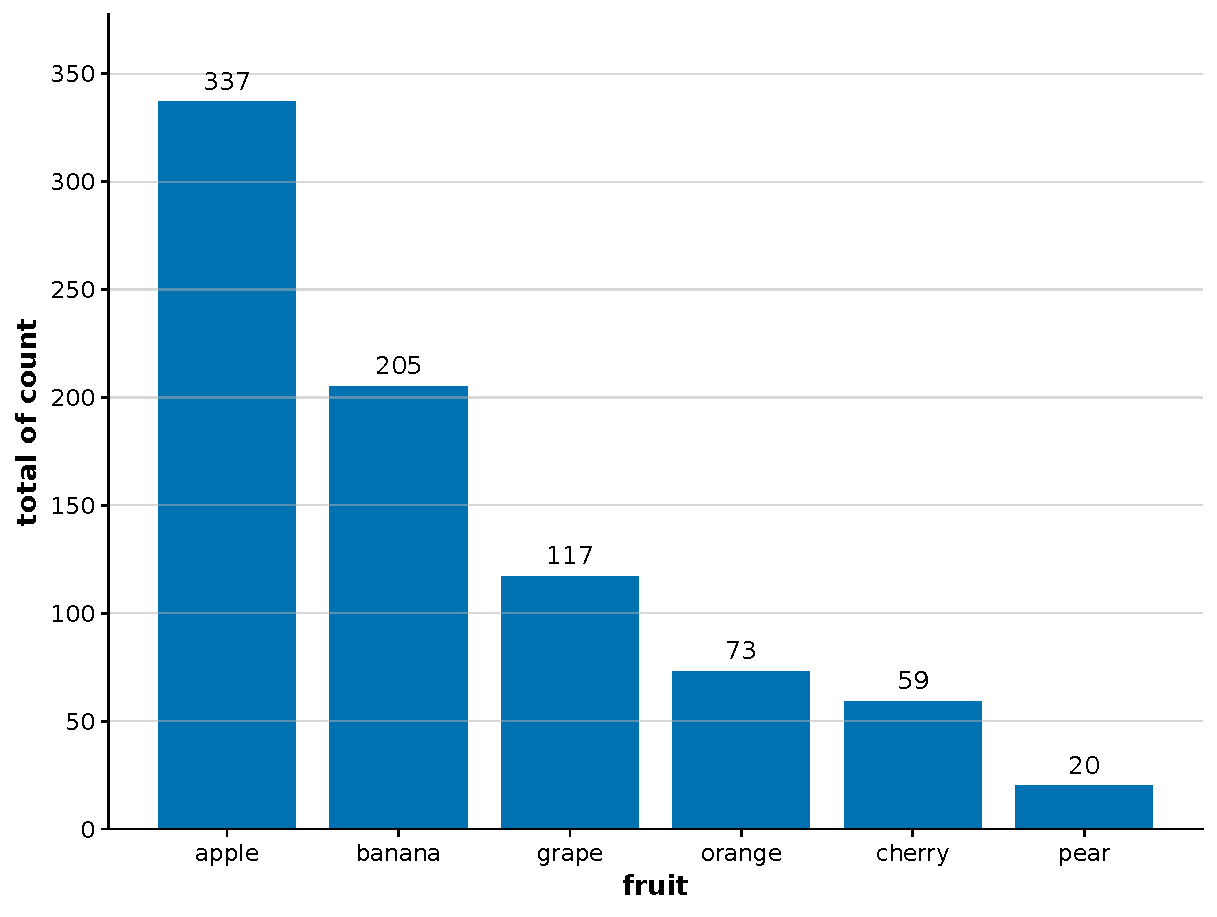
\includegraphics[width=0.72\textwidth,height=0.36\textheight,keepaspectratio]{figures/lesson12_example2_lesson12_fruit.pdf}
\captionof{figure}{Lesson 12, example 2: \code{lesson12\_\allowbreak{}fruit.\allowbreak{}png}.}
\end{minipage}\end{center}
\section*{Example 3}
A chart uses the table as it was when you made the chart. Table steps after it are for the next chart.
\begin{lstlisting}[style=py]
import simplydata as sdata
table = sdata.table(sdata.get_example("marks"))
table.keep_rows_where("class", is_equal_to="A")
all_tests = table.start_chart()
all_tests.draw_dots(x="hours", y="marks")
table.keep_rows_where("subject", is_equal_to="Maths")
maths = table.start_chart()
maths.draw_dots(x="hours", y="marks")
page = sdata.put_side_by_side(all_tests, maths, same_y=True)
page.save("lesson12_maths.png")
\end{lstlisting}
\whateachline
\begin{lineexplain}
  \item[1] Load simplydata.
  \item[2] Make a table of the marks.
  \item[3] Keep class A.
  \item[4] A chart of the table as it is now: every test of class A. \code{sdata.\allowbreak{}chart(table)} does the same.
  \item[5] Draw hours against marks.
  \item[6] A table step after the chart. The chart \code{all\_\allowbreak{}tests} does not change.
  \item[7] A second chart, of the table as it is now: only the Maths tests of class A.
  \item[8] Draw the same thing again.
  \item[9] Both charts on one page, with the same y-axis, so you can compare them.
  \item[10] Save the page.
\end{lineexplain}
\printedoutput{output/lesson12_example3.txt}
\begin{center}\begin{minipage}{\linewidth}\centering
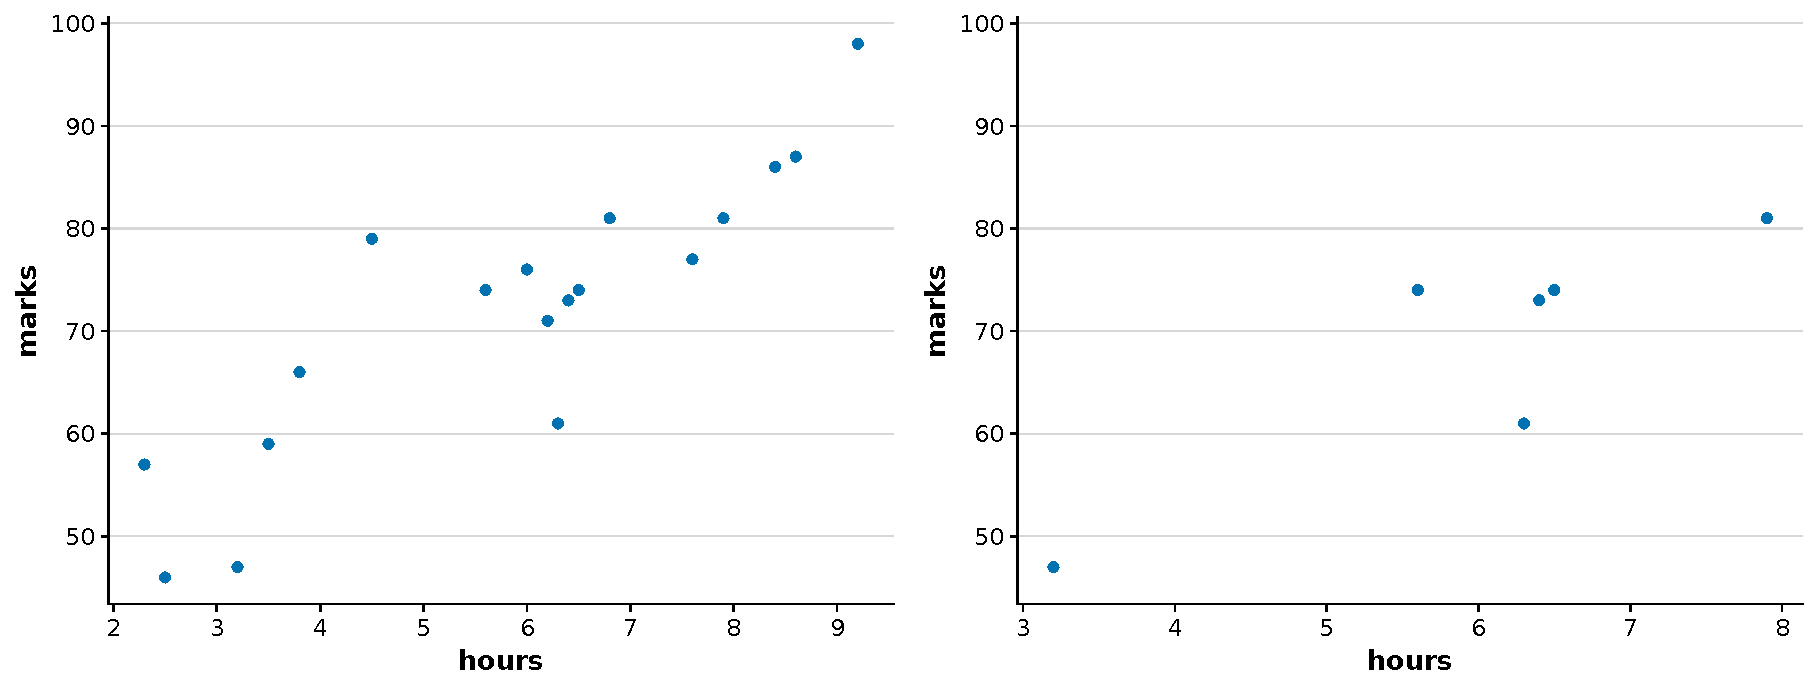
\includegraphics[width=0.72\textwidth,height=0.36\textheight,keepaspectratio]{figures/lesson12_example3_lesson12_maths.pdf}
\captionof{figure}{Lesson 12, example 3: \code{lesson12\_\allowbreak{}maths.\allowbreak{}png}.}
\end{minipage}\end{center}
\section*{Example 4}
Two tables can be joined: their rows are matched on a column they share.
\begin{lstlisting}[style=py]
import simplydata as sdata
table = sdata.table(sdata.get_example("marks"))
ages = {"name": ["Asha", "Ben", "Chen"], "age": [12, 13, 12]}
table.join_with(ages, using="name")
table.show_first_rows()
table.find_average_of("marks", for_each_group_in="age")
\end{lstlisting}
\whateachline
\begin{lineexplain}
  \item[1] Load simplydata.
  \item[2] Make a table of the marks.
  \item[3] A small table of ages, typed by hand: each column name, then its values.
  \item[4] Bring in the age, matching the rows on the name. Only children found in both tables stay.
  \item[5] Look: there is a new column, age.
  \item[6] The average mark at each age.
\end{lineexplain}
\printedoutput{output/lesson12_example4.txt}
\section*{Example 5}
Turning columns into rows makes a wide table long: the shape most charts like.
\begin{lstlisting}[style=py]
import simplydata as sdata
table = sdata.table({"name": ["Asha", "Ben", "Chen"], "test_1": [61, 73, 81], "test_2": [70, 68, 90]})
table.turn_columns_into_rows(["test_1", "test_2"], names_to="test", values_to="mark")
table.show_first_rows(6)
chart = table.start_chart()
chart.draw_bars(x="name", y="mark", colour="test")
chart.save("lesson12_tests.png")
\end{lstlisting}
\whateachline
\begin{lineexplain}
  \item[1] Load simplydata.
  \item[2] A small, wide table: two tests, one column for each.
  \item[3] Put the two tests under each other. The new column \code{\textquotedbl{}test\textquotedbl{}} says which test, and \code{\textquotedbl{}mark\textquotedbl{}} holds the mark. Each child now has two rows.
  \item[4] Look at the new, long shape.
  \item[5] Start a chart from it.
  \item[6] Both tests side by side for each child.
  \item[7] Save it.
\end{lineexplain}
\printedoutput{output/lesson12_example5.txt}
\begin{center}\begin{minipage}{\linewidth}\centering
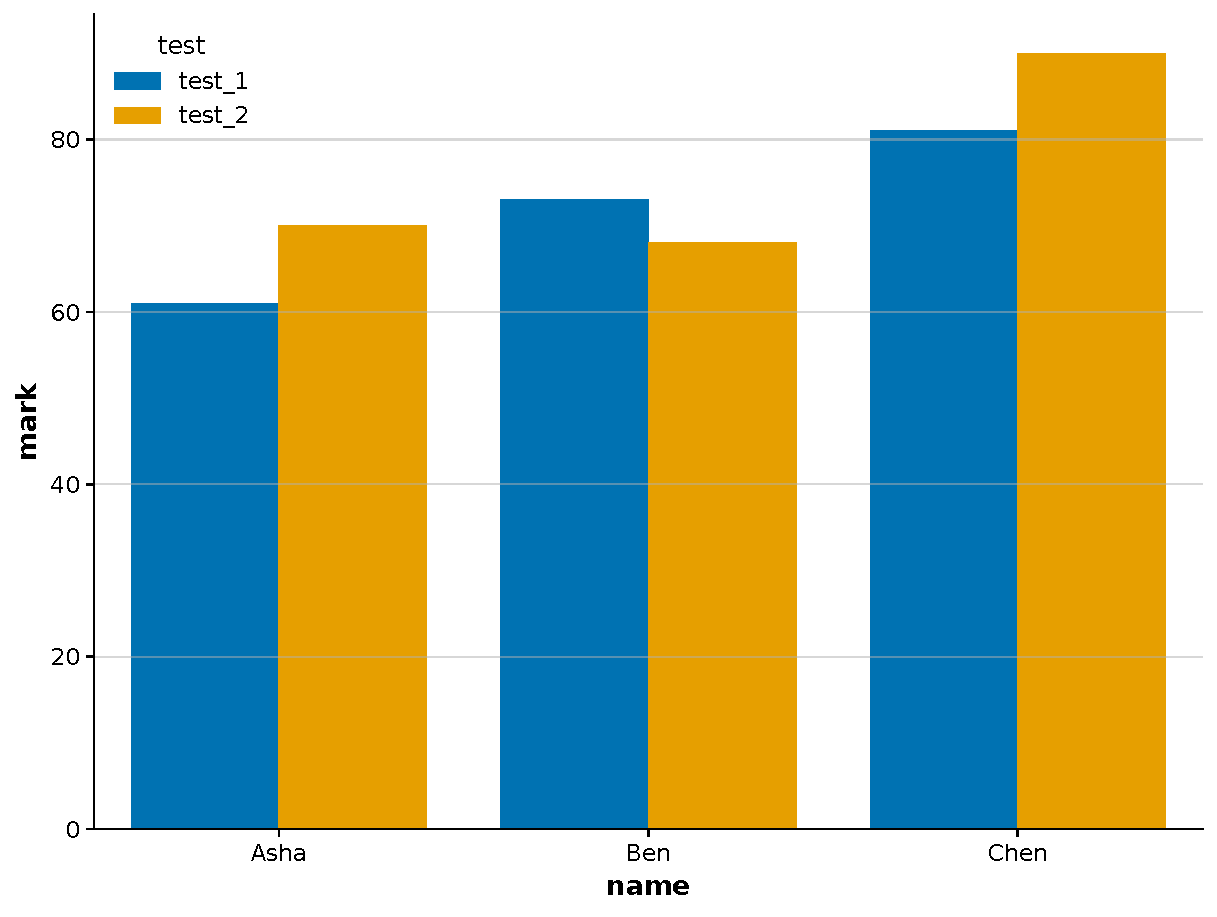
\includegraphics[width=0.72\textwidth,height=0.36\textheight,keepaspectratio]{figures/lesson12_example5_lesson12_tests.pdf}
\captionof{figure}{Lesson 12, example 5: \code{lesson12\_\allowbreak{}tests.\allowbreak{}png}.}
\end{minipage}\end{center}
\section*{Example 6}
\code{find\_\allowbreak{}summary\_\allowbreak{}of} gives several measures at once, and \code{every=} sums up dates by week, month or year.
\begin{lstlisting}[style=py]
import simplydata as sdata
table = sdata.table(sdata.get_example("shop"))
table.find_summary_of("sales", for_each_group_in="shop", show=["average", "median", "standard deviation", "count", "empty cells"])
table.find_total_of("sales", for_each_group_in="date", every="month")
table.find_percent_of_rows_where("sales", is_above=500, for_each_group_in="shop")
\end{lstlisting}
\whateachline
\begin{lineexplain}
  \item[1] Load simplydata.
  \item[2] Daily sales of two shops.
  \item[3] Five measures of each shop's sales in one tidy table. count counts the days with a number; empty cells counts the others.
  \item[4] The total sales of each month: \code{every=} puts the days of one month together.
  \item[5] On what percent of the days did each shop take more than 500? Each percent comes with its 95 \% confidence interval.
\end{lineexplain}
\printedoutput{output/lesson12_example6.txt}
\section*{Example 7}
A cross table puts one group down the side and another across the top. A correlation table compares many columns at once.
\begin{lstlisting}[style=py]
import simplydata as sdata
fruit = sdata.table(sdata.get_example("fruit"))
fruit.count_rows(for_each_group_in="shop", across="fruit")
fruit.count_different_values_in("fruit", for_each_group_in="shop")
marks = sdata.table(sdata.get_example("marks"))
marks.find_average_of("marks", for_each_group_in="class", across="subject")
marks.find_correlation_between("hours", "marks", "height")
\end{lstlisting}
\whateachline
\begin{lineexplain}
  \item[1] Load simplydata.
  \item[2] A table of fruit sales.
  \item[3] How many sales of each fruit in each shop: one row per shop, one column per fruit.
  \item[4] How many different fruits each shop sold.
  \item[5] A table of the marks.
  \item[6] The average mark of each class in each subject.
  \item[7] Every pair of the three columns at once: a correlation table, with the strongest pairs in words.
\end{lineexplain}
\printedoutput{output/lesson12_example7.txt}
\section*{Example 8}
More ways to sum up: percentiles, the most common value, and measures of shape.
\begin{lstlisting}[style=py]
import simplydata as sdata
marks = sdata.table(sdata.get_example("marks"))
marks.find_percentile_of("marks", 90, for_each_group_in="class")
marks.find_summary_of("marks", show=["median", "skewness", "coefficient of variation"], for_each_group_in="class")
school = sdata.table(sdata.get_example("school"))
school.find_most_common_of("days_absent")
\end{lstlisting}
\whateachline
\begin{lineexplain}
  \item[1] Load simplydata.
  \item[2] A table of the marks.
  \item[3] The 90th percentile: 90 \% of the marks are below it (86.3 in class A).
  \item[4] Skewness says if the values lean to one side (below 0: a longer tail of low marks); the coefficient of variation is the standard deviation divided by the average.
  \item[5] A table of pupils.
  \item[6] The most common number of days absent (the mode): 2.
\end{lineexplain}
\printedoutput{output/lesson12_example8.txt}
\section*{Example 9}
A z-score puts marks from different subjects on one scale: how many standard deviations a value lies above or below the average of its group.
\begin{lstlisting}[style=py]
import simplydata as sdata
table = sdata.table(sdata.get_example("marks"))
table.add_z_score_column("marks_z", from_column="marks", for_each_group_in="subject")
table.show_first_rows(3)
\end{lstlisting}
\whateachline
\begin{lineexplain}
  \item[1] Load simplydata.
  \item[2] A table of the marks.
  \item[3] A new column \code{\textquotedbl{}marks\_\allowbreak{}z\textquotedbl{}}: 0 is the average of that subject, 1 one standard deviation above it (SciPy zscore, as R \code{scale()}).
  \item[4] Asha's 77 in English is 1.09 standard deviations above the English average; her 66 in Science is a little below the Science average (-0.25).
\end{lineexplain}
\printedoutput{output/lesson12_example9.txt}
\begin{goodtoknow}
\begin{itemize}
  \item Correlation is not cause. Children who study more might also sleep more, or like the subject more; r only says that two columns go up and down together, not which one makes the other change.
  \item More summaries: \code{find\_\allowbreak{}median\_\allowbreak{}of}, \code{find\_\allowbreak{}total\_\allowbreak{}of}, \code{find\_\allowbreak{}smallest\_\allowbreak{}of}, \code{find\_\allowbreak{}biggest\_\allowbreak{}of}, \code{find\_\allowbreak{}standard\_\allowbreak{}deviation\_\allowbreak{}of} and \code{count\_\allowbreak{}rows}. Each one can take \code{for\_\allowbreak{}each\_\allowbreak{}group\_\allowbreak{}in=}.
  \item A chart never changes its table, and a table step never changes a chart you already made. So one cleaned table can feed many charts.
  \item \code{table.\allowbreak{}add\_\allowbreak{}rows\_\allowbreak{}from(other)} puts the rows of another table under this one. \code{turn\_\allowbreak{}rows\_\allowbreak{}into\_\allowbreak{}columns} does the opposite of \code{turn\_\allowbreak{}columns\_\allowbreak{}into\_\allowbreak{}rows}.
  \item Lesson 13 teaches numbers, and lesson 14 the statistical tests: is a difference real, and how big is it?
  \item Every summary skips empty cells and says how many it skipped. \code{find\_\allowbreak{}summary\_\allowbreak{}of} can also show \code{\textquotedbl{}variance\textquotedbl{}}, \code{\textquotedbl{}standard error\textquotedbl{}}, \code{\textquotedbl{}confidence interval\textquotedbl{}}, \code{\textquotedbl{}range\textquotedbl{}} and \code{\textquotedbl{}interquartile range\textquotedbl{}}.
\end{itemize}
\end{goodtoknow}
\begin{tryit}
\begin{enumerate}
  \item Make the fruit totals \code{for\_\allowbreak{}each\_\allowbreak{}group\_\allowbreak{}in=\textquotedbl{}shop\textquotedbl{}} instead. Which shop sold more?
  \item Work out the average temperature \code{for\_\allowbreak{}each\_\allowbreak{}group\_\allowbreak{}in=\textquotedbl{}city\textquotedbl{}} in the weather table and draw it as bars.
  \item Is there a link between height and marks? Use \code{find\_\allowbreak{}correlation\_\allowbreak{}between} to find out.
  \item Make a cross table of the average mark \code{for\_\allowbreak{}each\_\allowbreak{}group\_\allowbreak{}in=\textquotedbl{}subject\textquotedbl{}} \code{across=\textquotedbl{}class\textquotedbl{}}. Which class is best in Science?
\end{enumerate}
Worked solutions: page~\pageref{solutions:12}, or type \code{sdata.\allowbreak{}show\_\allowbreak{}lesson(12,\allowbreak{} solutions=True)}.
\end{tryit}
\par\noindent{\small\sffamily\textbf{Words in this lesson:} \hyperref[word:table.find-average-of]{\code{table.\allowbreak{}find\_\allowbreak{}average\_\allowbreak{}of()}}, \hyperref[word:table.find-biggest-of]{\code{table.\allowbreak{}find\_\allowbreak{}biggest\_\allowbreak{}of()}}, \hyperref[word:table.find-correlation-between]{\code{table.\allowbreak{}find\_\allowbreak{}correlation\_\allowbreak{}between()}}, \hyperref[word:table.find-total-of]{\code{table.\allowbreak{}find\_\allowbreak{}total\_\allowbreak{}of()}}, \hyperref[word:table.start-chart]{\code{table.\allowbreak{}start\_\allowbreak{}chart()}}, \hyperref[word:sdata.put-side-by-side]{\code{sdata.\allowbreak{}put\_\allowbreak{}side\_\allowbreak{}by\_\allowbreak{}side()}}, \hyperref[word:table.join-with]{\code{table.\allowbreak{}join\_\allowbreak{}with()}}, \hyperref[word:table.turn-columns-into-rows]{\code{table.\allowbreak{}turn\_\allowbreak{}columns\_\allowbreak{}into\_\allowbreak{}rows()}}, \hyperref[word:table.add-rows-from]{\code{table.\allowbreak{}add\_\allowbreak{}rows\_\allowbreak{}from()}}, \hyperref[word:table.find-summary-of]{\code{table.\allowbreak{}find\_\allowbreak{}summary\_\allowbreak{}of()}}, \hyperref[word:table.find-percent-of-rows-where]{\code{table.\allowbreak{}find\_\allowbreak{}percent\_\allowbreak{}of\_\allowbreak{}rows\_\allowbreak{}where()}}, \hyperref[word:table.count-rows]{\code{table.\allowbreak{}count\_\allowbreak{}rows()}}, \hyperref[word:table.count-different-values-in]{\code{table.\allowbreak{}count\_\allowbreak{}different\_\allowbreak{}values\_\allowbreak{}in()}}, \hyperref[word:table.find-percentile-of]{\code{table.\allowbreak{}find\_\allowbreak{}percentile\_\allowbreak{}of()}}, \hyperref[word:table.find-most-common-of]{\code{table.\allowbreak{}find\_\allowbreak{}most\_\allowbreak{}common\_\allowbreak{}of()}}.\par}

\chapter{Numbers: lists and grids of numbers}\label{lesson:13}
\begin{learnbox}
\begin{itemize}
  \item how to make a list of numbers, and a grid of them
  \item two ways to do maths: symbols make new numbers, words change the numbers you have
  \item how to keep some numbers, sum them up, and draw them
\end{itemize}
\end{learnbox}
\section*{Example 1}
Numbers are for when you have just numbers, not a table with named columns.
\begin{lstlisting}[style=py]
import simplydata as sdata
nums = sdata.numbers([12, 15, 9, 20, 14])
print(nums)
bigger = nums * 2
print(bigger)
nums.add(1)
nums.undo()
nums.keep_each_number_that(is_above=10)
nums.find_average()
nums.find_standard_deviation()
nums.show_steps()
\end{lstlisting}
\whateachline
\begin{lineexplain}
  \item[1] Load simplydata.
  \item[2] Make a list of five numbers and call it nums.
  \item[3] Look at them. The first line says how many there are.
  \item[4] Maths with symbols makes NEW numbers: every number times 2. nums itself does not change.
  \item[5] 24, 30, 18, 40 and 28.
  \item[6] Maths with words CHANGES the numbers you have: add 1 to each one.
  \item[7] Like a table, numbers can take back every word.
  \item[8] Keep only the numbers above 10. The same conditions as \code{keep\_\allowbreak{}rows\_\allowbreak{}where}: \code{is\_\allowbreak{}above}, \code{is\_\allowbreak{}below}, \code{is\_\allowbreak{}between} ...
  \item[9] The average of what is left, said in a sentence.
  \item[10] How spread out they are (divide by n - 1, as in pandas and R).
  \item[11] List the steps you did.
\end{lineexplain}
\printedoutput{output/lesson13_example1.txt}
\section*{Example 2}
Counting, random numbers and a chart.
\begin{lstlisting}[style=py]
import simplydata as sdata
months = sdata.numbers(1, to=12)
temps = sdata.numbers([4, 6, 9, 13, 17, 20, 22, 21, 17, 12, 8, 5])
chart = sdata.chart()
chart.draw_lines(x=months, y=temps, with_dots=True)
chart.save("lesson13_line.png")
heights = sdata.make_random_numbers(how_many=200, average=150, standard_deviation=8, with_seed=1)
heights.find_median()
heights.find_percentile(90)
chart = heights.start_chart()
chart.draw_histogram(x="value", with_bins=12)
chart.save("lesson13_heights.png")
\end{lstlisting}
\whateachline
\begin{lineexplain}
  \item[1] Load simplydata.
  \item[2] Count from 1 to 12. The end is included.
  \item[3] A temperature for each month.
  \item[4] Start an empty chart: the numbers go straight into the chart type.
  \item[5] Draw the temperatures as a line, month by month.
  \item[6] Save it.
  \item[7] 200 made-up heights that bunch around 150 in a bell shape (a normal distribution). \code{with\_\allowbreak{}seed=1} gives the same numbers every time, so others can repeat your work.
  \item[8] The middle height.
  \item[9] The height that 90 \% of them are below.
  \item[10] Start a chart from the numbers. Their column is called value.
  \item[11] Count how many heights fall in each range.
  \item[12] Save it. Can you see the bell shape?
\end{lineexplain}
\printedoutput{output/lesson13_example2.txt}
\begin{center}\begin{minipage}{\linewidth}\centering
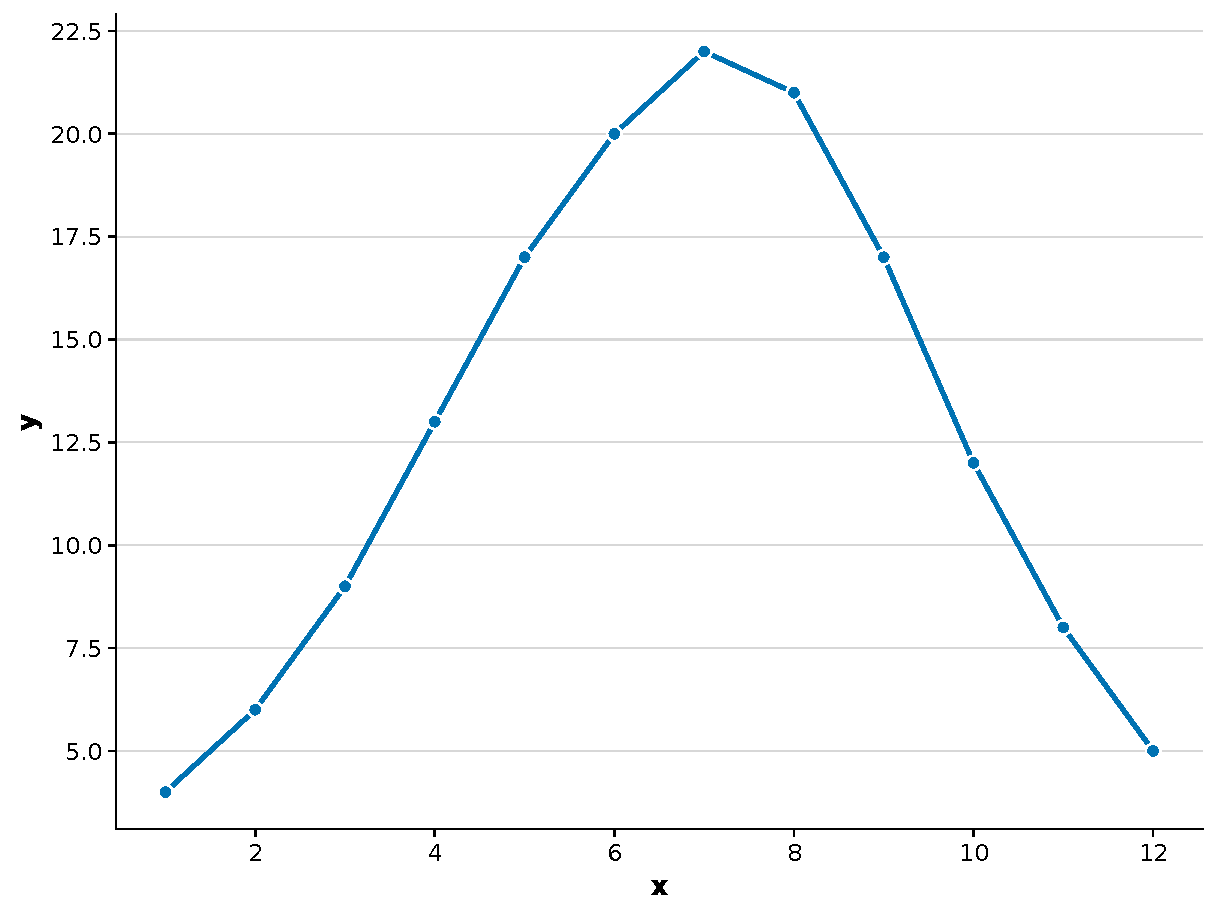
\includegraphics[width=0.48\textwidth,height=0.36\textheight,keepaspectratio]{figures/lesson13_example2_lesson13_line.pdf}\hfill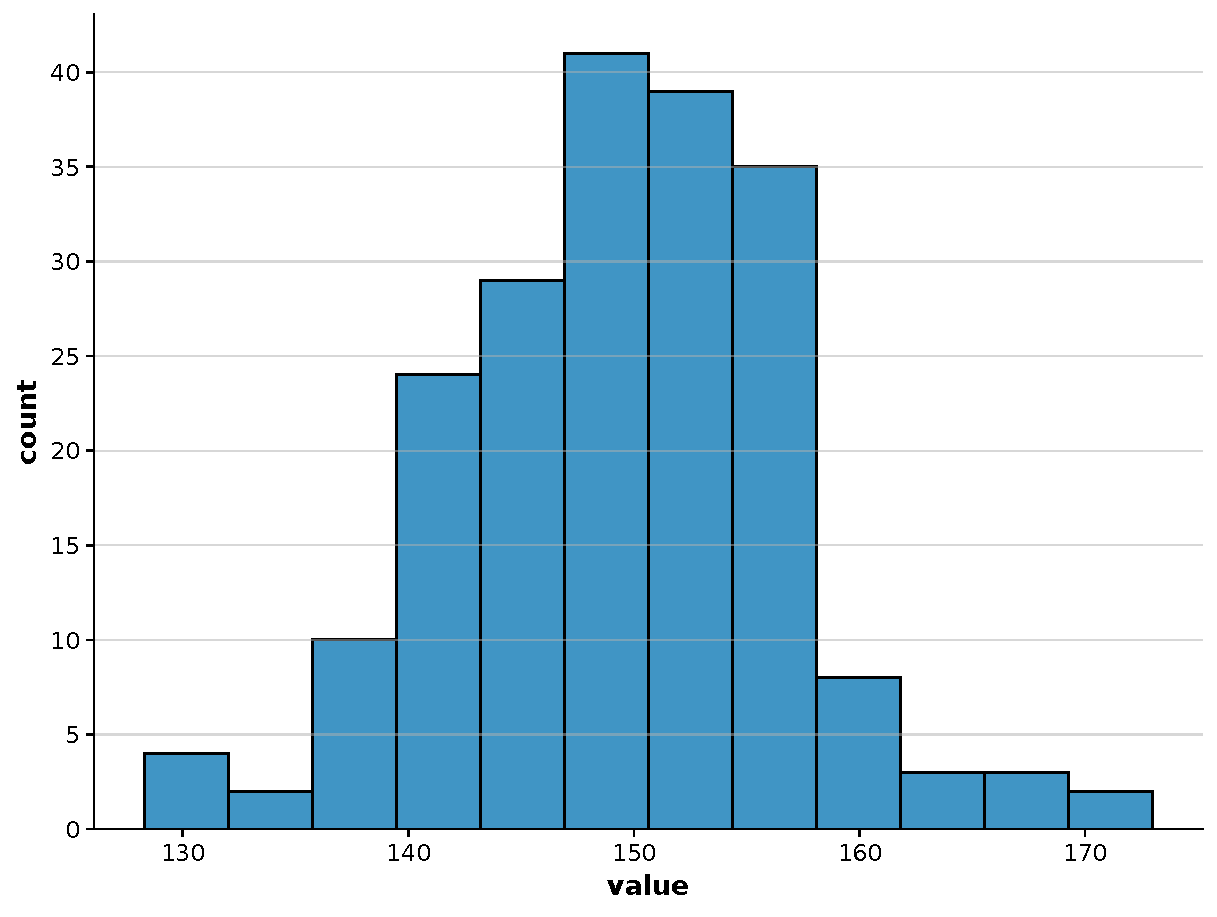
\includegraphics[width=0.48\textwidth,height=0.36\textheight,keepaspectratio]{figures/lesson13_example2_lesson13_heights.pdf}
\captionof{figure}{Lesson 13, example 2: \code{lesson13\_\allowbreak{}line.\allowbreak{}png} and \code{lesson13\_\allowbreak{}heights.\allowbreak{}png}.}
\end{minipage}\end{center}
\section*{Example 3}
A grid holds numbers in rows and columns. Positions count from 1.
\begin{lstlisting}[style=py]
import simplydata as sdata
grid = sdata.number_grid([[3, 5, 2], [8, 6, 4]])
print(grid.get_number_at(row=1, column=2))
grid.find_total(in_each="row")
grid.find_average(in_each="column")
grid.swap_rows_and_columns()
print(grid)
chart = grid.start_chart()
chart.draw_heatmap(with_numbers=True)
chart.save("lesson13_grid.png")
\end{lstlisting}
\whateachline
\begin{lineexplain}
  \item[1] Load simplydata.
  \item[2] A grid with 2 rows and 3 columns: one list for each row.
  \item[3] The number in row 1, column 2: 5.
  \item[4] The total of each row: 10 and 18.
  \item[5] The average of each column.
  \item[6] Rows become columns (in maths: the transpose).
  \item[7] Now 3 rows and 2 columns.
  \item[8] Start a chart from the grid.
  \item[9] One coloured square for each number, with the number written in.
  \item[10] Save it.
\end{lineexplain}
\printedoutput{output/lesson13_example3.txt}
\begin{center}\begin{minipage}{\linewidth}\centering
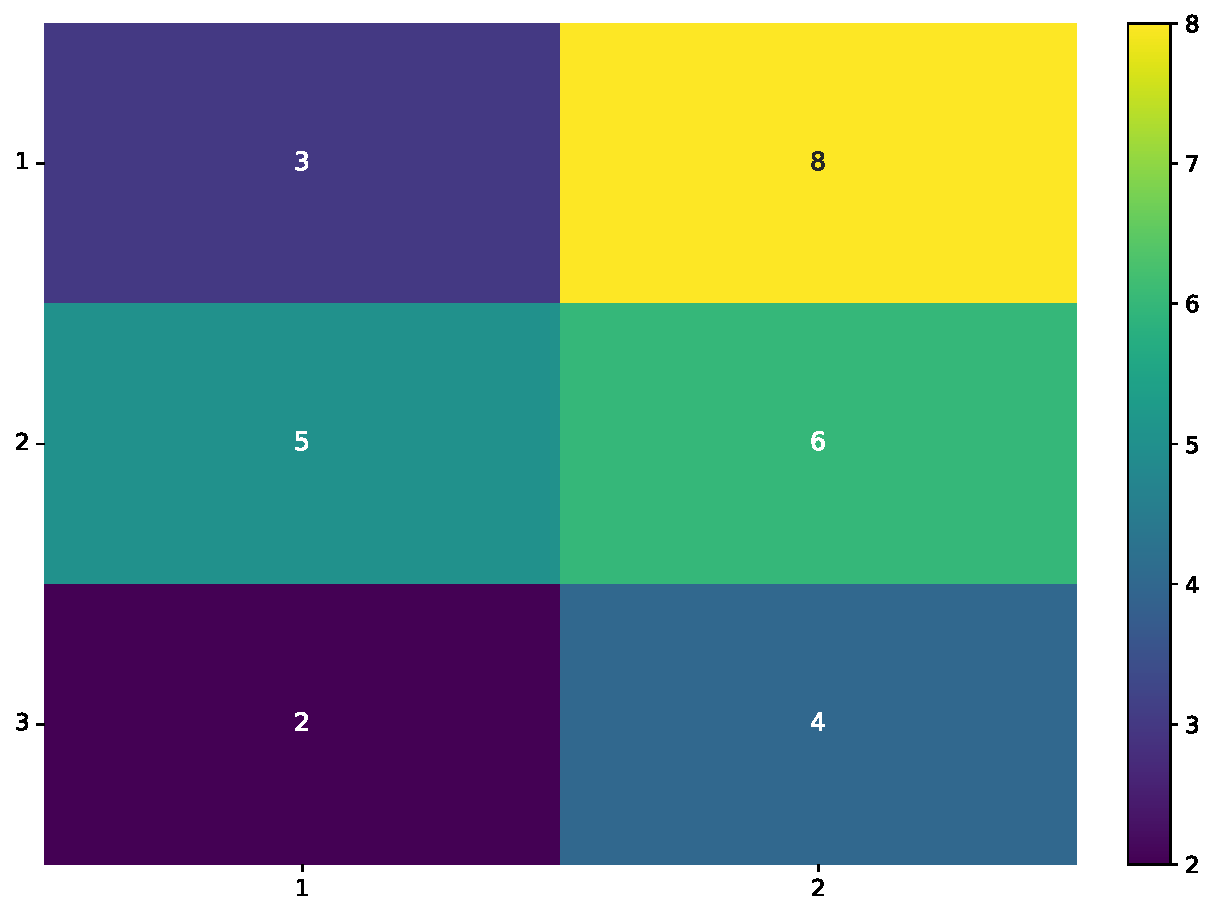
\includegraphics[width=0.72\textwidth,height=0.36\textheight,keepaspectratio]{figures/lesson13_example3_lesson13_grid.pdf}
\captionof{figure}{Lesson 13, example 3: \code{lesson13\_\allowbreak{}grid.\allowbreak{}png}.}
\end{minipage}\end{center}
\begin{goodtoknow}
\begin{itemize}
  \item The words follow the table words, with numbers in place of rows: \code{keep\_\allowbreak{}first\_\allowbreak{}numbers}, \code{remove\_\allowbreak{}empty\_\allowbreak{}numbers}, \code{fill\_\allowbreak{}empty\_\allowbreak{}numbers}, \code{show\_\allowbreak{}first\_\allowbreak{}numbers}.
  \item Summaries have no \_of, because there is no column to name: \code{nums.\allowbreak{}find\_\allowbreak{}average()}, not \code{table.\allowbreak{}find\_\allowbreak{}average\_\allowbreak{}of(\textquotedbl{}marks\textquotedbl{})}.
  \item A sum with no answer, such as dividing by 0 or the square root of a negative number, gives an empty value and a note, never a crash.
  \item \code{nums.\allowbreak{}turn\_\allowbreak{}into\_\allowbreak{}table()} turns numbers into a table, and \code{nums.\allowbreak{}as\_\allowbreak{}numpy()} gives a plain NumPy array if another Python tool needs one.
\end{itemize}
\end{goodtoknow}
\begin{tryit}
\begin{enumerate}
  \item Make the numbers 1 to 10, then square them in two ways: with ** 2 and with \code{raise\_\allowbreak{}to\_\allowbreak{}power(2)}.
  \item Make 6 dice throws with \code{sdata.\allowbreak{}make\_\allowbreak{}random\_\allowbreak{}numbers(how\_\allowbreak{}many=6,\allowbreak{} between=[1,\allowbreak{} 6],\allowbreak{} whole\_\allowbreak{}numbers=True,\allowbreak{} with\_\allowbreak{}seed=1)}. What is their total?
  \item Make a grid of 3 rows and 4 columns filled with 0: \code{sdata.\allowbreak{}number\_\allowbreak{}grid(rows=3,\allowbreak{} columns=4,\allowbreak{} filled\_\allowbreak{}with=0)}.
\end{enumerate}
Worked solutions: page~\pageref{solutions:13}, or type \code{sdata.\allowbreak{}show\_\allowbreak{}lesson(13,\allowbreak{} solutions=True)}.
\end{tryit}
\par\noindent{\small\sffamily\textbf{Words in this lesson:} \hyperref[word:sdata.numbers]{\code{sdata.\allowbreak{}numbers()}}, \hyperref[word:sdata.make-random-numbers]{\code{sdata.\allowbreak{}make\_\allowbreak{}random\_\allowbreak{}numbers()}}, \hyperref[word:sdata.number-grid]{\code{sdata.\allowbreak{}number\_\allowbreak{}grid()}}, \hyperref[word:nums.add]{\code{nums.\allowbreak{}add()}}, \hyperref[word:nums.undo]{\code{nums.\allowbreak{}undo()}}, \hyperref[word:nums.keep-each-number-that]{\code{nums.\allowbreak{}keep\_\allowbreak{}each\_\allowbreak{}number\_\allowbreak{}that()}}, \hyperref[word:nums.find-average]{\code{nums.\allowbreak{}find\_\allowbreak{}average()}}, \hyperref[word:nums.find-standard-deviation]{\code{nums.\allowbreak{}find\_\allowbreak{}standard\_\allowbreak{}deviation()}}, \hyperref[word:nums.find-median]{\code{nums.\allowbreak{}find\_\allowbreak{}median()}}, \hyperref[word:nums.find-percentile]{\code{nums.\allowbreak{}find\_\allowbreak{}percentile()}}, \hyperref[word:nums.start-chart]{\code{nums.\allowbreak{}start\_\allowbreak{}chart()}}, \hyperref[word:grid.get-number-at]{\code{grid.\allowbreak{}get\_\allowbreak{}number\_\allowbreak{}at()}}, \hyperref[word:grid.swap-rows-and-columns]{\code{grid.\allowbreak{}swap\_\allowbreak{}rows\_\allowbreak{}and\_\allowbreak{}columns()}}, \hyperref[word:nums.show-steps]{\code{nums.\allowbreak{}show\_\allowbreak{}steps()}}.\par}

\chapter{Statistical tests: real difference, or chance?}\label{lesson:14}
\begin{learnbox}
\begin{itemize}
  \item how big a difference is, and how sure the data are: the effect and its interval first
  \item what a p-value means: first by shuffling the labels, then from the usual formula
  \item how to compare the averages of groups, and which groups differ
  \item how to compare counts and measurements of the same people, and how to fit a line or a formula
\end{itemize}
\end{learnbox}
\section*{Example 1}
Start with the question \code{\textquotedbl{}how big?\textquotedbl{}}: the difference between two groups, and how sure the data are about it.
\begin{lstlisting}[style=py]
import simplydata as sdata
school = sdata.table(sdata.get_example("school"))
school.find_average_of("sleep", for_each_group_in="passed", interval=95)
school.compare_averages_of("sleep", for_each_group_in="passed")
\end{lstlisting}
\whateachline
\begin{lineexplain}
  \item[1] Load simplydata.
  \item[2] A table of pupils.
  \item[3] The average hours of sleep of the pupils who passed and of those who did not, each with its 95 \% confidence interval: the range the true average is very likely in.
  \item[4] Read the first sentence first: the pupils who did not pass slept about half an hour less (0.485 hours), and the 95 \% interval of the difference goes from 0.196 to 0.774 hours. That is the effect, and how sure the data are about it. The p-value comes after it.
\end{lineexplain}
\printedoutput{output/lesson14_example1.txt}
\section*{Example 2}
Where does a p-value come from? Shuffle the labels, and count.
\begin{lstlisting}[style=py]
import simplydata as sdata
school = sdata.table(sdata.get_example("school"))
school.compare_averages_of("sleep", for_each_group_in="passed", p_value_by="shuffling")
\end{lstlisting}
\whateachline
\begin{lineexplain}
  \item[1] Load simplydata.
  \item[2] A table of pupils.
  \item[3] Imagine that passing had nothing to do with sleep. Then the labels \code{\textquotedbl{}yes\textquotedbl{}} and \code{\textquotedbl{}no\textquotedbl{}} could be shuffled among the pupils and nothing would change. simplydata shuffles them 9999 times and counts how often the shuffled difference is as big as the real one: about 1 time in 1000 (p = 0.001). That count is the p-value. The p-value in the part before came from a formula (the t distribution), a shortcut for the same count: here it is the same, p = 0.001.
\end{lineexplain}
\printedoutput{output/lesson14_example2.txt}
\section*{Example 3}
Groups almost never have exactly the same average. A test asks: is the difference bigger than chance alone would often give?
\begin{lstlisting}[style=py]
import simplydata as sdata
table = sdata.table(sdata.get_example("marks"))
table.compare_averages_of("marks", for_each_group_in="class")
table.compare_each_pair_of("marks", for_each_group_in="class")
table.compare_averages_of("marks", for_each_group_in="subject", based_on="ranks")
\end{lstlisting}
\whateachline
\begin{lineexplain}
  \item[1] Load simplydata.
  \item[2] Make a table of the marks.
  \item[3] Do the three classes really differ in their average mark? The answer comes in words. The p-value says how often differences this big or bigger would turn up in studies like this one if the classes were truly the same: here in about 3 of 100 (p = 0.028). It is not the chance that the classes are the same. With three or more groups this test is also called Welch's ANOVA; with two groups, a t-test.
  \item[4] Which classes differ? Each pair gets its own t-test (Welch's). Testing many pairs makes a false alarm more likely, so the p-values are adjusted (Holm's method).
  \item[5] \code{based\_\allowbreak{}on=\textquotedbl{}ranks\textquotedbl{}} puts the marks in order and compares the places instead (a Kruskal-Wallis test, or Mann-Whitney for two groups). It is safer when groups are small and the values are not bell-shaped.
\end{lineexplain}
\printedoutput{output/lesson14_example3.txt}
\section*{Example 4}
Counts can be compared too: does how often something happens differ between groups?
\begin{lstlisting}[style=py]
import simplydata as sdata
table = sdata.table(sdata.get_example("marks"))
table.add_group_column("result", from_column="marks", cut_at=[60], names=["below 60", "60 or more"])
table.compare_counts_of("result", for_each_group_in="class")
\end{lstlisting}
\whateachline
\begin{lineexplain}
  \item[1] Load simplydata.
  \item[2] Make a table of the marks.
  \item[3] A new column that says if each mark is below 60 or not.
  \item[4] Do the classes differ in how many marks are 60 or more? This counts the rows for each class and result and uses the chi-square test. Cramer's V says how strong the link is, from 0 (none) to 1.
\end{lineexplain}
\printedoutput{output/lesson14_example4.txt}
\section*{Example 5}
A fit finds the line or formula that follows the data best, and says how sure it is.
\begin{lstlisting}[style=py]
import simplydata as sdata
table = sdata.table(sdata.get_example("marks"))
table.fit_line(x="hours", y="marks")
growth = sdata.table(sdata.get_example("growth"))
growth.keep_rows_where("country", is_equal_to="Applia")
growth.fit_formula("population = a * exp(b * (year - 2000))")
\end{lstlisting}
\whateachline
\begin{lineexplain}
  \item[1] Load simplydata.
  \item[2] Make a table of the marks.
  \item[3] How much do the marks go up for each extra hour of study? This is linear regression by least squares. R squared says how much of the differences in marks the line explains.
  \item[4] A second table, with the growth data.
  \item[5] Keep one country.
  \item[6] Fit a formula you write yourself. Names that are columns (population, year) are data; the others (a and b) are found by simplydata. Here b is the growth rate each year. This is nonlinear least squares.
\end{lineexplain}
\printedoutput{output/lesson14_example5.txt}
\section*{Example 6}
Before a test, look at the shape of the values and at values far from the rest. After many tests, adjust the p-values.
\begin{lstlisting}[style=py]
import simplydata as sdata
table = sdata.table(sdata.get_example("marks"))
table.compare_shape_to("marks", "normal", for_each_group_in="class")
table.show_rows_with_outliers("marks", for_each_group_in="class")
pairs = table.find_correlation_between("hours", "marks", "height", show="each pair")
pairs.add_adjusted_p_value_column(method="holm")
pairs.show()
\end{lstlisting}
\whateachline
\begin{lineexplain}
  \item[1] Load simplydata.
  \item[2] Make a table of the marks.
  \item[3] Do the marks of each class look bell-shaped (normal)? The Shapiro-Wilk test answers for each class. Tests on averages work best with bell-shaped values, or with many values.
  \item[4] The rows whose mark is far from the rest of its class, by Tukey's rule (the one box plots use): here one mark of 33 in class B. The table does not change.
  \item[5] Test three pairs of columns at once: a table with one row per pair and its p-value.
  \item[6] With many tests, one of them looks real by chance more often. Holm's adjustment keeps the chance of even one false alarm at 5 \%.
  \item[7] The p-values and the adjusted ones, side by side.
\end{lineexplain}
\printedoutput{output/lesson14_example6.txt}
\section*{Example 7}
Some questions are about spread, or about counts compared with what you expect.
\begin{lstlisting}[style=py]
import simplydata as sdata
table = sdata.table(sdata.get_example("marks"))
table.compare_spreads_of("marks", for_each_group_in="class")
table.compare_each_pair_of("marks", for_each_group_in="class", test="tukey")
school = sdata.table(sdata.get_example("school"))
school.compare_counts_to("breakfast", expected={"yes": 0.6, "no": 0.4})
school.compare_percent_to("passed", value="yes", percent=50)
\end{lstlisting}
\whateachline
\begin{lineexplain}
  \item[1] Load simplydata.
  \item[2] Make a table of the marks.
  \item[3] Are the marks of one class more spread out? The data cannot tell: differences in spread this big would turn up in about 91 of 100 studies even if the spreads were the same (p = 0.91).
  \item[4] Tukey's test compares every pair at once: only A and C differ (p = 0.020).
  \item[5] A table of pupils.
  \item[6] Did 60 \% eat breakfast, as a survey said? 115 of 180 is close enough (p = 0.29).
  \item[7] Did half the pupils pass? 43.3 \% did; if truly half passed, a difference this big would turn up in about 9 of 100 studies (p = 0.086), so the data cannot tell.
\end{lineexplain}
\printedoutput{output/lesson14_example7.txt}
\section*{Example 8}
When the same people are measured three times, compare the measurements within each person.
\begin{lstlisting}[style=py]
import simplydata as sdata
clinic = sdata.table(sdata.get_example("clinic"))
clinic.compare_matched_columns("pain_week_0", "pain_week_4", "pain_week_8")
\end{lstlisting}
\whateachline
\begin{lineexplain}
  \item[1] Load simplydata.
  \item[2] A table of patients.
  \item[3] Each patient scored the pain at week 0, 4 and 8, one column each. \code{compare\_\allowbreak{}matched\_\allowbreak{}columns} compares the three columns within each patient (the Friedman test, on ranks): the median pain falls from 6 to 5 to 4, far more than chance would give (p \textless{} 0.0001). For two columns, \code{compare\_\allowbreak{}before\_\allowbreak{}and\_\allowbreak{}after} does the same.
\end{lineexplain}
\printedoutput{output/lesson14_example8.txt}
\begin{goodtoknow}
\begin{itemize}
  \item The idea behind every test: imagine there is no real difference (this is called the null hypothesis). The p-value says how often a difference this big or bigger would turn up then, in studies like yours: p = 0.03 is \code{\textquotedbl{}about 3 of 100 studies\textquotedbl{}}. It is not the chance that there is no difference, and every test says it in that one sentence.
  \item A p-value does not say how big or important the difference is: the effect size does that (omega-squared, Cohen's d, Cramer's V ...). And a large p-value does not show that there is no difference. It only means these data cannot tell.
  \item A 95 \% confidence interval is the range the true value is very likely in. A narrow one means the data pin the value down well; a wide one means you need more data.
  \item Each test gives back a one-row table with all its numbers, so you can save it: result = \code{table.\allowbreak{}compare\_\allowbreak{}averages\_\allowbreak{}of(.\allowbreak{}.\allowbreak{}.\allowbreak{})}, then \code{result.\allowbreak{}save(\textquotedbl{}test.\allowbreak{}csv\textquotedbl{})}.
  \item Also: \code{compare\_\allowbreak{}before\_\allowbreak{}and\_\allowbreak{}after} for two measurements of the same thing (a paired t-test), and \code{compare\_\allowbreak{}average\_\allowbreak{}to} for one average against a number you choose.
  \item \code{remove\_\allowbreak{}rows\_\allowbreak{}with\_\allowbreak{}outliers} removes such rows. Say in your report which rule removed how many rows, and never remove a value only because it spoils the result.
  \item \code{method=\textquotedbl{}benjamini-hochberg\textquotedbl{}} adjusts for many tests more gently: it controls the share of false alarms among your findings (the false discovery rate).
\end{itemize}
\end{goodtoknow}
\begin{tryit}
\begin{enumerate}
  \item Compare the average marks \code{for\_\allowbreak{}each\_\allowbreak{}group\_\allowbreak{}in=\textquotedbl{}subject\textquotedbl{}}. Could the differences be chance?
  \item Is the average temperature different between the cities of \code{sdata.\allowbreak{}get\_\allowbreak{}example(\textquotedbl{}weather\textquotedbl{})}?
  \item Fit a straight line of \code{\textquotedbl{}forest\textquotedbl{}} against \code{\textquotedbl{}year\textquotedbl{}} in \code{sdata.\allowbreak{}get\_\allowbreak{}example(\textquotedbl{}growth\textquotedbl{})} for one country.
  \item Remove the rows with outliers in \code{\textquotedbl{}marks\textquotedbl{}} \code{for\_\allowbreak{}each\_\allowbreak{}group\_\allowbreak{}in=\textquotedbl{}class\textquotedbl{}}, then compare the average marks \code{for\_\allowbreak{}each\_\allowbreak{}group\_\allowbreak{}in=\textquotedbl{}class\textquotedbl{}} again. Did the answer change?
\end{enumerate}
Worked solutions: page~\pageref{solutions:14}, or type \code{sdata.\allowbreak{}show\_\allowbreak{}lesson(14,\allowbreak{} solutions=True)}.
\end{tryit}
\par\noindent{\small\sffamily\textbf{Words in this lesson:} \hyperref[word:table.compare-averages-of]{\code{table.\allowbreak{}compare\_\allowbreak{}averages\_\allowbreak{}of()}}, \hyperref[word:table.compare-each-pair-of]{\code{table.\allowbreak{}compare\_\allowbreak{}each\_\allowbreak{}pair\_\allowbreak{}of()}}, \hyperref[word:table.compare-counts-of]{\code{table.\allowbreak{}compare\_\allowbreak{}counts\_\allowbreak{}of()}}, \hyperref[word:table.fit-line]{\code{table.\allowbreak{}fit\_\allowbreak{}line()}}, \hyperref[word:table.fit-formula]{\code{table.\allowbreak{}fit\_\allowbreak{}formula()}}, \hyperref[word:table.add-group-column]{\code{table.\allowbreak{}add\_\allowbreak{}group\_\allowbreak{}column()}}, \hyperref[word:table.compare-shape-to]{\code{table.\allowbreak{}compare\_\allowbreak{}shape\_\allowbreak{}to()}}, \hyperref[word:table.show-rows-with-outliers]{\code{table.\allowbreak{}show\_\allowbreak{}rows\_\allowbreak{}with\_\allowbreak{}outliers()}}, \hyperref[word:table.add-adjusted-p-value-column]{\code{table.\allowbreak{}add\_\allowbreak{}adjusted\_\allowbreak{}p\_\allowbreak{}value\_\allowbreak{}column()}}, \hyperref[word:table.remove-rows-with-outliers]{\code{table.\allowbreak{}remove\_\allowbreak{}rows\_\allowbreak{}with\_\allowbreak{}outliers()}}, \hyperref[word:table.compare-spreads-of]{\code{table.\allowbreak{}compare\_\allowbreak{}spreads\_\allowbreak{}of()}}, \hyperref[word:table.compare-counts-to]{\code{table.\allowbreak{}compare\_\allowbreak{}counts\_\allowbreak{}to()}}, \hyperref[word:table.compare-percent-to]{\code{table.\allowbreak{}compare\_\allowbreak{}percent\_\allowbreak{}to()}}, \hyperref[word:table.compare-matched-columns]{\code{table.\allowbreak{}compare\_\allowbreak{}matched\_\allowbreak{}columns()}}.\par}

\chapter{A whole analysis: from a question to a figure}\label{lesson:15}
\begin{learnbox}
\begin{itemize}
  \item how to put all the lessons together: open, look, clean, sum up, test, draw and save
  \item how to make a figure with panels A and B, ready for a report or a paper
  \item how \code{show\_\allowbreak{}steps()} writes down what you did, in plain words
  \item how to hand your table to pandas or Polars, and back
\end{itemize}
\end{learnbox}
\section*{Example 1}
A whole analysis with one question: do children who study longer get better marks, and do the classes differ? One table feeds two charts, and the two charts become one figure.
\begin{lstlisting}[style=py]
import simplydata as sdata
table = sdata.table(sdata.get_example("marks"))
table.describe_columns()
table.remove_rows_with_empty_cells_in()
table.find_average_of("marks", for_each_group_in="class")
table.compare_averages_of("marks", for_each_group_in="class")
a = table.start_chart()
a.draw_boxes(x="class", y="marks")
a.draw_all_dots(x="class", y="marks")
a.label_y("Mark (out of 100)")
b = table.start_chart()
b.draw_dots(x="hours", y="marks", colour="class")
b.fit_line(with_confidence_band=True)
b.label_x("Hours of study")
figure = sdata.put_in_rows_and_columns(a, b, per_row=2, with_letters=True)
figure.write_title_on_top("Marks, classes and hours of study")
figure.use_style("paper")
figure.set_size(width=17, height=8, unit="cm")
figure.save("lesson15_figure.pdf")
figure.save("lesson15_figure.tif", resolution=600)
table.save("lesson15_clean.xlsx")
table.show_steps()
\end{lstlisting}
\whateachline
\begin{lineexplain}
  \item[1] Load simplydata.
  \item[2] Open the data. For your own file: \code{sdata.\allowbreak{}table(\textquotedbl{}results.\allowbreak{}xlsx\textquotedbl{})}.
  \item[3] Look: what is in each column, and are any cells empty?
  \item[4] Clean: remove the rows with an empty cell. The practice table has none, so nothing is removed.
  \item[5] Sum up: the average mark of each class.
  \item[6] Test: could the differences between the classes be chance?
  \item[7] Chart A, from the cleaned table.
  \item[8] The marks of each class as boxes.
  \item[9] Every mark as a dot, on top of the boxes.
  \item[10] Name its y-axis.
  \item[11] Chart B, from the same table.
  \item[12] Hours of study against marks, one colour per class.
  \item[13] A straight line for each class, with its 95 \% confidence band.
  \item[14] Name its x-axis.
  \item[15] Both charts on one page, with A and B at the top left.
  \item[16] A title for the whole page.
  \item[17] A quiet look that suits a paper.
  \item[18] The size a journal asks for: 17 cm wide (a full page width) and 8 cm high.
  \item[19] Save the figure as a PDF: sharp at any size.
  \item[20] And as a \code{.\allowbreak{}tif} picture with 600 dots per inch, as many journals ask.
  \item[21] Save the cleaned table that the figure was drawn from.
  \item[22] Every table step in plain words, in order: a good start for the methods part of your report.
\end{lineexplain}
\printedoutput{output/lesson15_example1.txt}
\begin{center}\begin{minipage}{\linewidth}\centering
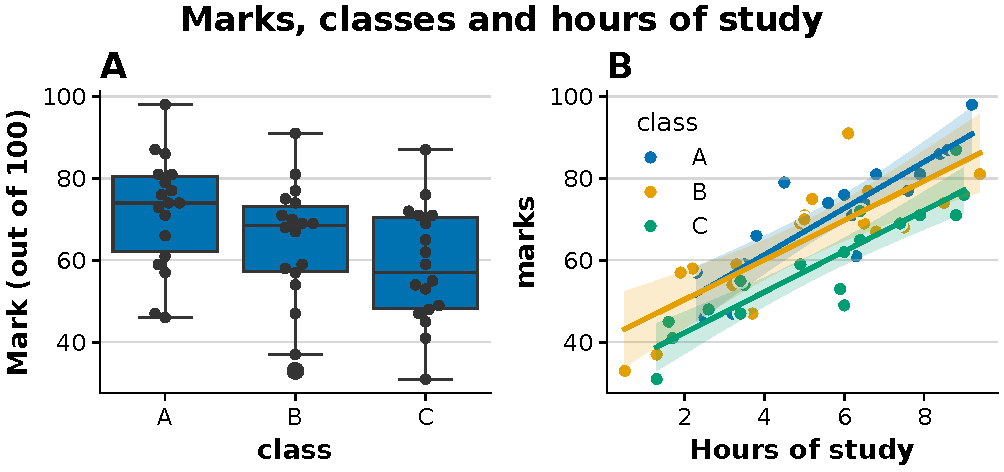
\includegraphics[width=0.72\textwidth,height=0.36\textheight,keepaspectratio]{figures/lesson15_example1_lesson15_figure.pdf}
\captionof{figure}{Lesson 15, example 1: \code{lesson15\_\allowbreak{}figure.\allowbreak{}pdf}.}
\end{minipage}\end{center}
\section*{Example 2}
Two questions about two tables give two charts. \code{sdata.\allowbreak{}put\_\allowbreak{}in\_\allowbreak{}rows\_\allowbreak{}and\_\allowbreak{}columns} puts them on one page.
\begin{lstlisting}[style=py]
import simplydata as sdata
weather = sdata.table(sdata.get_example("weather"))
weather.keep_rows_where("city", is_equal_to="Rainbridge")
rain = weather.start_chart()
rain.draw_bars(x="month", y="rain")
rain.draw_line_at_y(100, labelled="100 mm")
growth = sdata.table(sdata.get_example("growth"))
forest = growth.start_chart()
forest.draw_lines(x="year", y="forest", colour="country")
forest.label_y("Forest (% of the land)")
page = sdata.put_in_rows_and_columns(rain, forest, per_row=2, with_letters=True)
page.save("lesson15_two_tables.png")
\end{lstlisting}
\whateachline
\begin{lineexplain}
  \item[1] Load simplydata.
  \item[2] Table 1: the weather.
  \item[3] Keep one city.
  \item[4] A chart of it, called rain.
  \item[5] Its rain through the year.
  \item[6] A line at 100 mm.
  \item[7] Table 2: four countries.
  \item[8] A chart of it, called forest.
  \item[9] Their forest over the years.
  \item[10] Name the y-axis.
  \item[11] Both charts on one page, with letters.
  \item[12] Save the page.
\end{lineexplain}
\printedoutput{output/lesson15_example2.txt}
\begin{center}\begin{minipage}{\linewidth}\centering
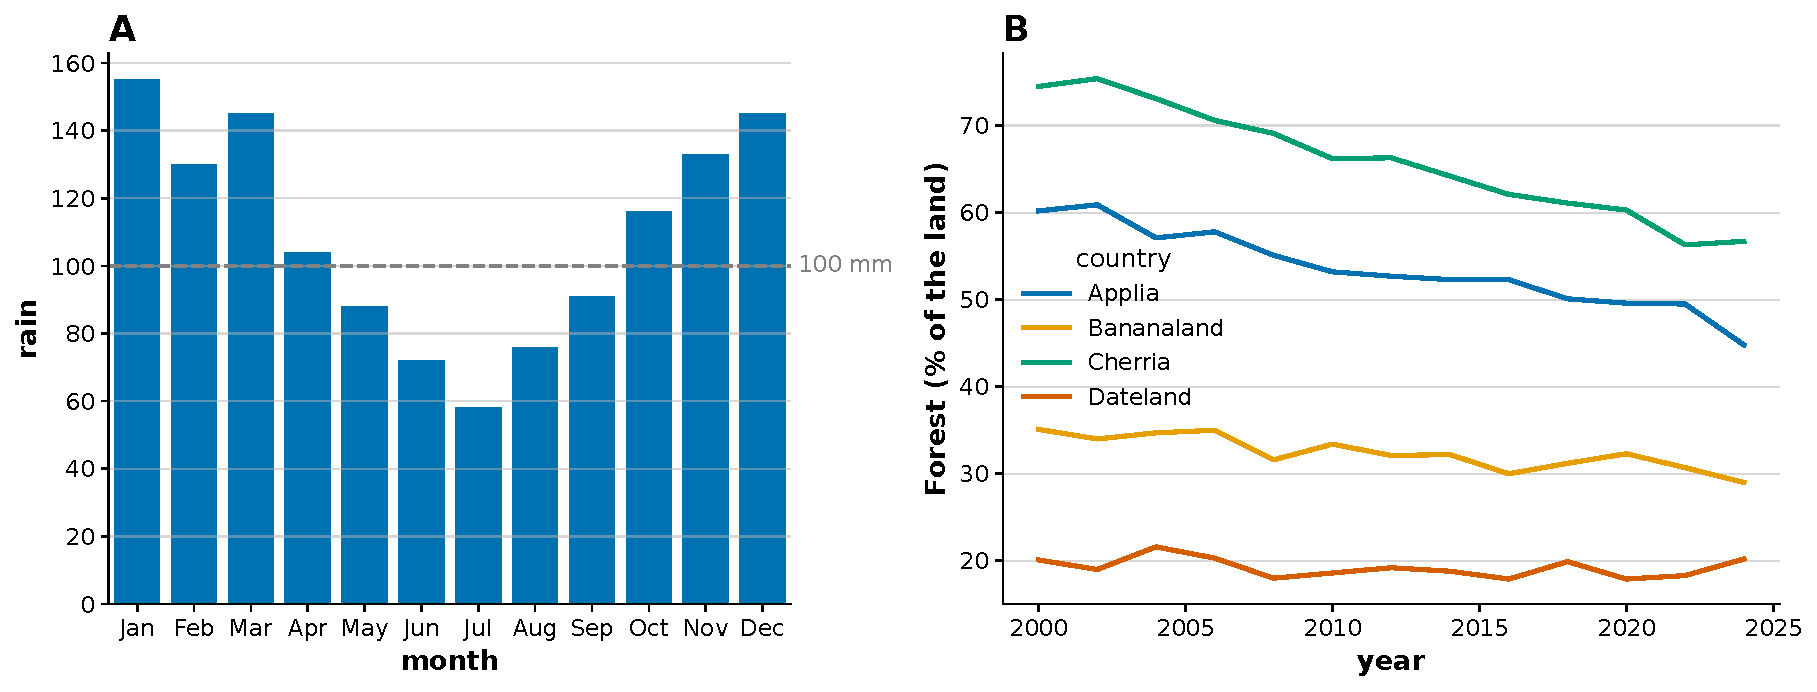
\includegraphics[width=0.72\textwidth,height=0.36\textheight,keepaspectratio]{figures/lesson15_example2_lesson15_two_tables.pdf}
\captionof{figure}{Lesson 15, example 2: \code{lesson15\_\allowbreak{}two\_\allowbreak{}tables.\allowbreak{}png}.}
\end{minipage}\end{center}
\section*{Example 3}
A table goes to pandas or Polars and back whenever another Python tool needs it.
\begin{lstlisting}[style=py]
import simplydata as sdata
table = sdata.table(sdata.get_example("weather"))
table.keep_rows_where("city", is_equal_to="Rainbridge")
df = table.as_pandas()
print(df["rain"].max())
again = sdata.table(df)
chart = sdata.chart(df)
chart.draw_bars(x="month", y="rain")
chart.save("lesson15_rain.png")
\end{lstlisting}
\whateachline
\begin{lineexplain}
  \item[1] Load simplydata.
  \item[2] A table of the weather.
  \item[3] Keep one city.
  \item[4] A plain pandas DataFrame (\code{table.\allowbreak{}as\_\allowbreak{}polars()} gives a Polars one).
  \item[5] Any pandas code works on it.
  \item[6] And back: \code{sdata.\allowbreak{}table} takes a pandas or Polars table you already have.
  \item[7] \code{sdata.\allowbreak{}chart} takes one too.
  \item[8] Draw it.
  \item[9] Save the chart.
\end{lineexplain}
\printedoutput{output/lesson15_example3.txt}
\begin{center}\begin{minipage}{\linewidth}\centering
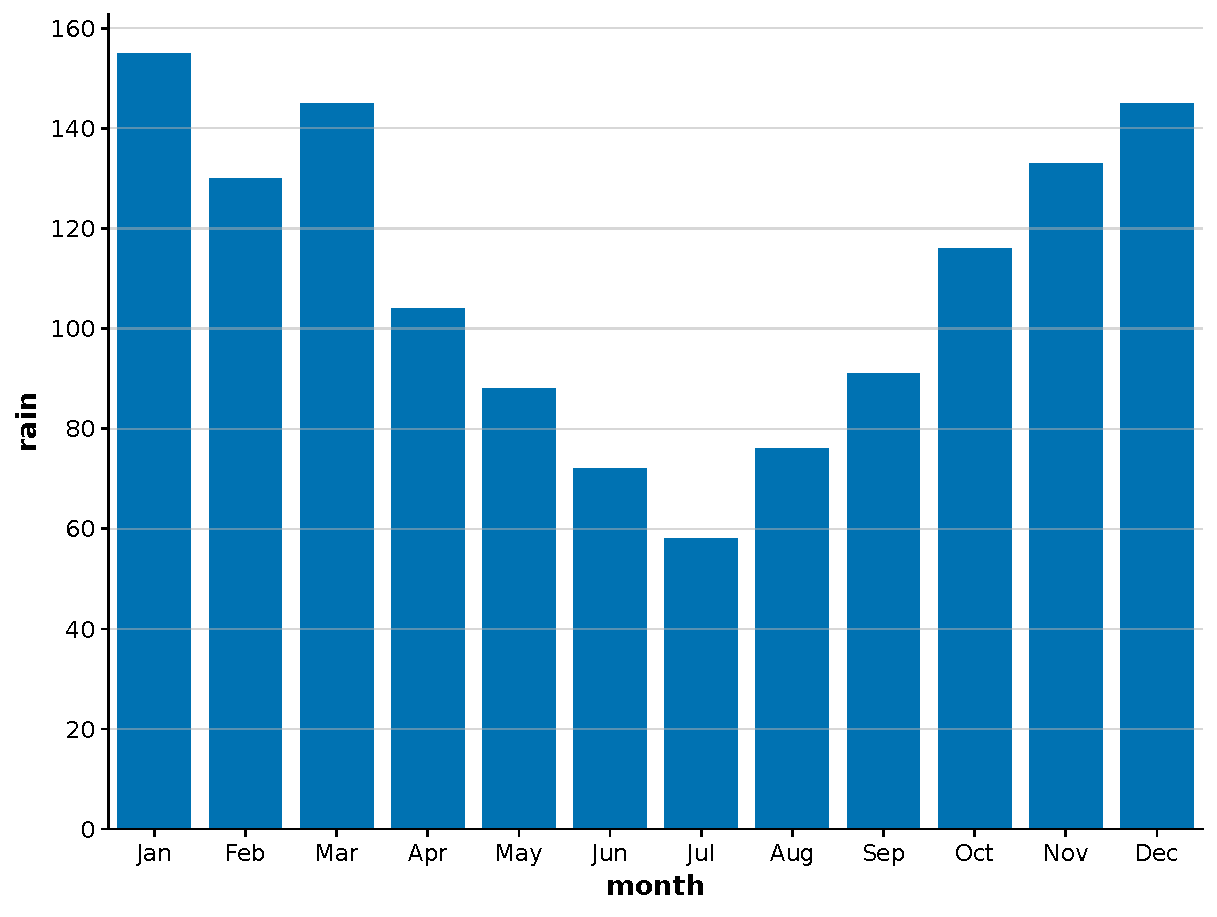
\includegraphics[width=0.72\textwidth,height=0.36\textheight,keepaspectratio]{figures/lesson15_example3_lesson15_rain.pdf}
\captionof{figure}{Lesson 15, example 3: \code{lesson15\_\allowbreak{}rain.\allowbreak{}png}.}
\end{minipage}\end{center}
\begin{goodtoknow}
\begin{itemize}
  \item Every analysis follows the same plan: open, look, clean, sum up, test, draw, words, save. Lessons 1 to 14 taught each part; this lesson puts them together.
  \item The table and the charts are separate objects, as in pandas and matplotlib: one cleaned table can feed many charts, and each chart keeps the rows the table had when the chart was made.
  \item \code{table.\allowbreak{}save} saves the table, and \code{chart.\allowbreak{}save} or \code{page.\allowbreak{}save} the picture. Save both, so anyone can check the figure against its data.
  \item \code{table.\allowbreak{}show\_\allowbreak{}steps()} lists the table steps. Together with the chart lines of your program, it says everything you did.
  \item simplydata words never need \code{as\_\allowbreak{}pandas()}; it is only for other tools.
\end{itemize}
\end{goodtoknow}
\begin{tryit}
\begin{enumerate}
  \item Do a whole analysis of \code{sdata.\allowbreak{}get\_\allowbreak{}example(\textquotedbl{}weather\textquotedbl{})}: look at it, compare the average rain \code{for\_\allowbreak{}each\_\allowbreak{}group\_\allowbreak{}in=\textquotedbl{}city\textquotedbl{}}, draw the rain of each city as boxes, and save the chart and the table.
  \item Make a second chart of the temperature, then put the two charts together with \code{sdata.\allowbreak{}put\_\allowbreak{}side\_\allowbreak{}by\_\allowbreak{}side(.\allowbreak{}.\allowbreak{}.\allowbreak{},\allowbreak{} with\_\allowbreak{}letters=True)}.
  \item Read the \code{show\_\allowbreak{}steps()} of your table out loud. Would someone else understand what you did?
\end{enumerate}
Worked solutions: page~\pageref{solutions:15}, or type \code{sdata.\allowbreak{}show\_\allowbreak{}lesson(15,\allowbreak{} solutions=True)}.
\end{tryit}
\par\noindent{\small\sffamily\textbf{Words in this lesson:} \hyperref[word:sdata.table]{\code{sdata.\allowbreak{}table()}}, \hyperref[word:table.describe-columns]{\code{table.\allowbreak{}describe\_\allowbreak{}columns()}}, \hyperref[word:table.remove-rows-with-empty-cells-in]{\code{table.\allowbreak{}remove\_\allowbreak{}rows\_\allowbreak{}with\_\allowbreak{}empty\_\allowbreak{}cells\_\allowbreak{}in()}}, \hyperref[word:table.compare-averages-of]{\code{table.\allowbreak{}compare\_\allowbreak{}averages\_\allowbreak{}of()}}, \hyperref[word:table.start-chart]{\code{table.\allowbreak{}start\_\allowbreak{}chart()}}, \hyperref[word:draw-boxes]{\code{chart.\allowbreak{}draw\_\allowbreak{}boxes()}}, \hyperref[word:draw-all-dots]{\code{chart.\allowbreak{}draw\_\allowbreak{}all\_\allowbreak{}dots()}}, \hyperref[word:draw-dots]{\code{chart.\allowbreak{}draw\_\allowbreak{}dots()}}, \hyperref[word:fit-line]{\code{chart.\allowbreak{}fit\_\allowbreak{}line()}}, \hyperref[word:sdata.put-in-rows-and-columns]{\code{sdata.\allowbreak{}put\_\allowbreak{}in\_\allowbreak{}rows\_\allowbreak{}and\_\allowbreak{}columns()}}, \hyperref[word:use-style]{\code{chart.\allowbreak{}use\_\allowbreak{}style()}}, \hyperref[word:table.save]{\code{table.\allowbreak{}save()}}, \hyperref[word:table.show-steps]{\code{table.\allowbreak{}show\_\allowbreak{}steps()}}, \hyperref[word:table.as-pandas]{\code{table.\allowbreak{}as\_\allowbreak{}pandas()}}, \hyperref[word:sdata.chart]{\code{sdata.\allowbreak{}chart()}}.\par}

\chapter{Models: explain one column from several others}\label{lesson:16}
\begin{learnbox}
\begin{itemize}
  \item how to explain one column from several others at once (multiple regression)
  \item how to explain a yes/no column (logistic regression) and a column of counts (Poisson regression)
  \item how to allow for groups such as schools (a mixed model)
  \item how to use rows with empty cells without guessing once (multiple imputation)
  \item how to say how much a column changes the chance of yes (a risk ratio, not only an odds ratio)
\end{itemize}
\end{learnbox}
\begin{needsr}Only \code{explain(.\allowbreak{}.\allowbreak{}.\allowbreak{},\allowbreak{} empty\_\allowbreak{}cells=\textquotedbl{}multiple imputation\textquotedbl{})} needs R: it pools its results with R (mice). The rest of the lesson needs no R. That option and the other R words run R's own code, the same code R users run. Install it once: pip install \code{\textquotedbl{}simplydata[r]\textquotedbl{}}, then R from https://cran.r-project.org, then in R: \code{install.\allowbreak{}packages(c(\textquotedbl{}vegan\textquotedbl{},\allowbreak{} \textquotedbl{}survival\textquotedbl{},\allowbreak{} \textquotedbl{}mice\textquotedbl{},\allowbreak{} \textquotedbl{}emmeans\textquotedbl{}))}. Without R these words print a message that says what to install.\end{needsr}
\section*{Example 1}
Marks depend on more than one thing. \code{explain()} looks at several columns together, so each effect is the effect with the other columns held fixed.
\begin{lstlisting}[style=py]
import simplydata as sdata
table = sdata.table(sdata.get_example("school"))
table.explain("marks", using=["hours", "sleep", "breakfast"])
table.explain("marks", using=["hours * breakfast"])
\end{lstlisting}
\whateachline
\begin{lineexplain}
  \item[1] Load simplydata.
  \item[2] Pupils in 12 schools: study, sleep, breakfast and marks.
  \item[3] Explain the marks from hours of study, hours of sleep and breakfast. Each extra hour of study goes with about 2.7 more marks, each extra hour of sleep with 2.3 more, and breakfast with 3.2 more, each with its 95 \% confidence interval and p-value. This is a linear model (multiple regression) by least squares.
  \item[4] hours * breakfast also asks: does the effect of study depend on breakfast? That is an interaction. Here the data cannot tell: about 31 of 100 studies would show this much if there were truly none (p = 0.31).
\end{lineexplain}
\printedoutput{output/lesson16_example1.txt}
\section*{Example 2}
Not every column is a number to explain. A yes/no column needs the chance of yes, and a count needs a model for counts.
\begin{lstlisting}[style=py]
import simplydata as sdata
table = sdata.table(sdata.get_example("school"))
table.explain("passed", using=["hours", "breakfast"], outcome="yes or no")
table.explain("days_absent", using=["hours", "sleep"], outcome="counts")
table.add_predicted_column("marks", using=["hours", "breakfast"])
table.show_first_rows(5)
\end{lstlisting}
\whateachline
\begin{lineexplain}
  \item[1] Load simplydata.
  \item[2] The school table.
  \item[3] Did the pupil pass? \code{outcome=\textquotedbl{}yes or no\textquotedbl{}} is logistic regression. Each extra hour of study multiplies the odds of passing by 1.66 (an odds ratio).
  \item[4] Days absent are counts (0, 1, 2 ...). \code{outcome=\textquotedbl{}counts\textquotedbl{}} is Poisson regression; each extra hour of study multiplies the expected days absent by 0.88 (a rate ratio).
  \item[5] Add a column \code{\textquotedbl{}predicted marks\textquotedbl{}}: what the model expects for each pupil.
  \item[6] Look at the marks next to the predicted marks.
\end{lineexplain}
\printedoutput{output/lesson16_example2.txt}
\section*{Example 3}
Pupils in the same school are alike in ways the columns do not show. A mixed model allows for that, and multiple imputation uses the rows with empty cells.
\begin{lstlisting}[style=py]
import simplydata as sdata
table = sdata.table(sdata.get_example("school"))
table.explain("marks", using=["hours", "breakfast"], grouped_by="school")
table.explain("marks", using=["hours", "sleep", "breakfast"], empty_cells="multiple imputation")
\end{lstlisting}
\whateachline
\begin{lineexplain}
  \item[1] Load simplydata.
  \item[2] The school table.
  \item[3] A mixed model: each school gets its own starting level (a random intercept). About 39 \% of the differences the columns do not explain lie between schools (the ICC).
  \item[4] 19 pupils did not say how long they slept. Instead of leaving them out, multiple imputation fills the empty cells 20 times, fits the model to each filled-in table and pools the 20 answers (Rubin's rules), so the extra uncertainty is counted.
\end{lineexplain}
\printedoutput{output/lesson16_example3.txt}
\section*{Example 4}
An odds ratio is not a risk ratio. When yes is common, the odds ratio is further from 1 than the change in the chance itself, and readers often take it for the chance.
\begin{lstlisting}[style=py]
import simplydata as sdata
table = sdata.table(sdata.get_example("school"))
table.explain("passed", using=["hours", "breakfast"], outcome="yes or no")
table.explain("passed", using=["hours", "breakfast"], outcome="yes or no", show="risk ratios")
\end{lstlisting}
\whateachline
\begin{lineexplain}
  \item[1] Load simplydata.
  \item[2] The school table.
  \item[3] Odds ratios, as in part 2. 43 \% of the pupils passed, so the printout ends with a note: an odds ratio is not a risk ratio here, and \code{show=\textquotedbl{}risk ratios\textquotedbl{}} gives risk ratios.
  \item[4] \code{show=\textquotedbl{}risk ratios\textquotedbl{}} gives risk ratios (modified Poisson regression): each extra hour of study multiplies the chance of passing by 1.21, where the odds ratio was 1.66. Say in words what 1.21 means: with one more hour of study, the chance of passing is about a fifth higher.
\end{lineexplain}
\printedoutput{output/lesson16_example4.txt}
\begin{goodtoknow}
\begin{itemize}
  \item Each effect in \code{explain()} holds the other columns fixed: the effect of sleep is the effect for pupils who study the same number of hours and have the same breakfast.
  \item A text column such as breakfast is compared with its first group in A to Z order (here \code{\textquotedbl{}no\textquotedbl{}}); the answer says which group is the baseline.
  \item An odds ratio above 1 means higher odds of yes; a rate ratio above 1 means more counts. 1 means no difference.
  \item If counts vary much more than a Poisson model expects (overdispersion), simplydata says so and suggests \code{outcome=\textquotedbl{}counts (overdispersed)\textquotedbl{}}; it never switches by itself.
  \item \code{grouped\_\allowbreak{}by=} is for rows that come in groups: pupils in schools, measurements on the same animal, samples from the same site. Without it, the p-values are too small.
  \item Multiple imputation needs the empty cells to be explainable by the other columns (missing at random). Say in your report how many cells were empty and how they were handled.
  \item \code{grouped\_\allowbreak{}by=} works out of the box (statsmodels comes with simplydata). Multiple imputation pools its results in R, so it needs R (see the box at the start).
  \item A risk ratio of 1.21 means the chance of yes is 21 \% higher. Report risk ratios when yes is common (more than about 1 in 10 rows); simplydata says when that is the case.
  \item More outcomes for later, all in the manual and the dictionary: \code{\textquotedbl{}yes or no (overdispersed)\textquotedbl{}} (yes counts out of tries that vary a lot), \code{\textquotedbl{}counts with many zeros that vary a lot\textquotedbl{}} and \code{\textquotedbl{}counts in two steps\textquotedbl{}} (first zero or not, then how many).
\end{itemize}
\end{goodtoknow}
\begin{tryit}
\begin{enumerate}
  \item Explain \code{\textquotedbl{}marks\textquotedbl{}} using \code{\textquotedbl{}hours\textquotedbl{}} and \code{\textquotedbl{}school\textquotedbl{}} (school as a column of groups). Which schools differ from School A, and is school as a whole important?
  \item Explain \code{\textquotedbl{}passed\textquotedbl{}} using \code{\textquotedbl{}hours\textquotedbl{}} and \code{\textquotedbl{}sleep\textquotedbl{}} with \code{outcome=\textquotedbl{}yes or no\textquotedbl{}}.
  \item Explain \code{\textquotedbl{}days\_\allowbreak{}absent\textquotedbl{}} using \code{\textquotedbl{}hours\textquotedbl{}} and \code{\textquotedbl{}breakfast\textquotedbl{}} with \code{outcome=\textquotedbl{}counts\textquotedbl{}}. Does breakfast matter?
  \item In the clinic table, explain \code{\textquotedbl{}caught\_\allowbreak{}infection\textquotedbl{}} using \code{\textquotedbl{}ward\textquotedbl{}} and \code{\textquotedbl{}patient\_\allowbreak{}days\textquotedbl{}} with \code{outcome=\textquotedbl{}yes or no\textquotedbl{}}, first as odds ratios and then with \code{show=\textquotedbl{}risk ratios\textquotedbl{}}. Which is further from 1?
\end{enumerate}
Worked solutions: page~\pageref{solutions:16}, or type \code{sdata.\allowbreak{}show\_\allowbreak{}lesson(16,\allowbreak{} solutions=True)}.
\end{tryit}
\par\noindent{\small\sffamily\textbf{Words in this lesson:} \hyperref[word:table.explain]{\code{table.\allowbreak{}explain()}}, \hyperref[word:table.add-predicted-column]{\code{table.\allowbreak{}add\_\allowbreak{}predicted\_\allowbreak{}column()}}, \hyperref[word:table.show-first-rows]{\code{table.\allowbreak{}show\_\allowbreak{}first\_\allowbreak{}rows()}}.\par}

\chapter{Patterns across many columns}\label{lesson:17}
\begin{learnbox}
\begin{itemize}
  \item how to sum up many columns in two new ones (principal components)
  \item how to measure how different rows are (Bray-Curtis and other distances)
  \item how to draw a map of the rows (NMDS) and test groups on all columns at once (PERMANOVA)
  \item how to find groups of similar rows (clustering)
\end{itemize}
\end{learnbox}
\begin{needsr}\code{add\_\allowbreak{}nmds()}, \code{compare\_\allowbreak{}profiles\_\allowbreak{}of()} and \code{add\_\allowbreak{}clusters()} with k-means (the default) run R's own code, the same code R users run. Install it once: pip install \code{\textquotedbl{}simplydata[r]\textquotedbl{}}, then R from https://cran.r-project.org, then in R: \code{install.\allowbreak{}packages(c(\textquotedbl{}vegan\textquotedbl{},\allowbreak{} \textquotedbl{}survival\textquotedbl{},\allowbreak{} \textquotedbl{}mice\textquotedbl{},\allowbreak{} \textquotedbl{}emmeans\textquotedbl{}))}. Without R these words print a message that says what to install.\end{needsr}
\section*{Example 1}
Ten plant counts per plot are too many to look at one by one. Principal components make a few new columns that hold most of the spread.
\begin{lstlisting}[style=py]
import simplydata as sdata
table = sdata.table(sdata.get_example("meadow"))
table.add_principal_components(how_many=2)
chart = table.start_chart()
chart.draw_dots(x="PC1", y="PC2", colour="grazed")
chart.save("lesson17_pca.png")
\end{lstlisting}
\whateachline
\begin{lineexplain}
  \item[1] Load simplydata.
  \item[2] Plants counted in 30 plots, half of them grazed by sheep.
  \item[3] Principal component analysis (PCA): adds PC1 and PC2. PC1 holds 30 \% of the spread, PC2 15 \%. The printout says which plants weigh most in each.
  \item[4] Start a chart.
  \item[5] Each plot is a dot; grazed and ungrazed plots sit apart.
  \item[6] Save it.
\end{lineexplain}
\printedoutput{output/lesson17_example1.txt}
\begin{center}\begin{minipage}{\linewidth}\centering
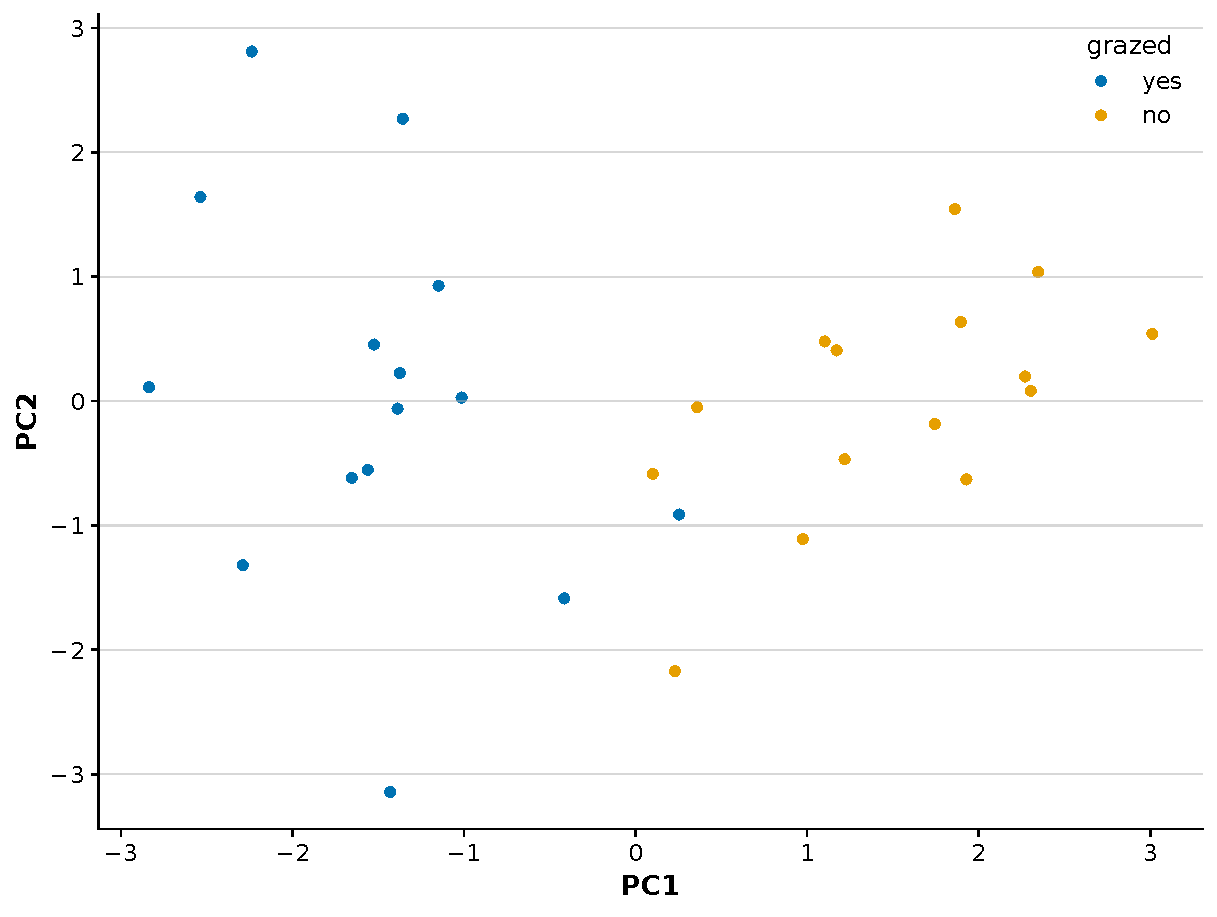
\includegraphics[width=0.72\textwidth,height=0.36\textheight,keepaspectratio]{figures/lesson17_example1_lesson17_pca.pdf}
\captionof{figure}{Lesson 17, example 1: \code{lesson17\_\allowbreak{}pca.\allowbreak{}png}.}
\end{minipage}\end{center}
\section*{Example 2}
Ecologists compare plots by how different their make-up is. Bray-Curtis is the usual distance for counts, and NMDS draws a map that keeps the order of the distances.
\begin{lstlisting}[style=py]
import simplydata as sdata
table = sdata.table(sdata.get_example("meadow"))
distances = table.find_distances_between_rows(measure="bray-curtis", names="plot")
distances.show_first_rows(3)
table.add_nmds(measure="bray-curtis")
table.compare_profiles_of(for_each_group_in="grazed")
chart = table.start_chart()
chart.draw_dots(x="NMDS1", y="NMDS2", colour="grazed")
chart.save("lesson17_nmds.png")
\end{lstlisting}
\whateachline
\begin{lineexplain}
  \item[1] Load simplydata.
  \item[2] The meadow table.
  \item[3] A table of the Bray-Curtis distance between every pair of plots: 0 means the same plants in the same numbers, 1 means nothing in common.
  \item[4] Look at the first rows.
  \item[5] Non-metric multidimensional scaling (NMDS): adds NMDS1 and NMDS2. The stress (0.195) says how well the map keeps the distances: usable.
  \item[6] Do grazed and ungrazed plots differ in make-up? PERMANOVA tests all ten plants at once: grazing explains 25 \% of the differences (p = 0.001).
  \item[7] Start a chart.
  \item[8] The NMDS map.
  \item[9] Save it.
\end{lineexplain}
\printedoutput{output/lesson17_example2.txt}
\begin{center}\begin{minipage}{\linewidth}\centering
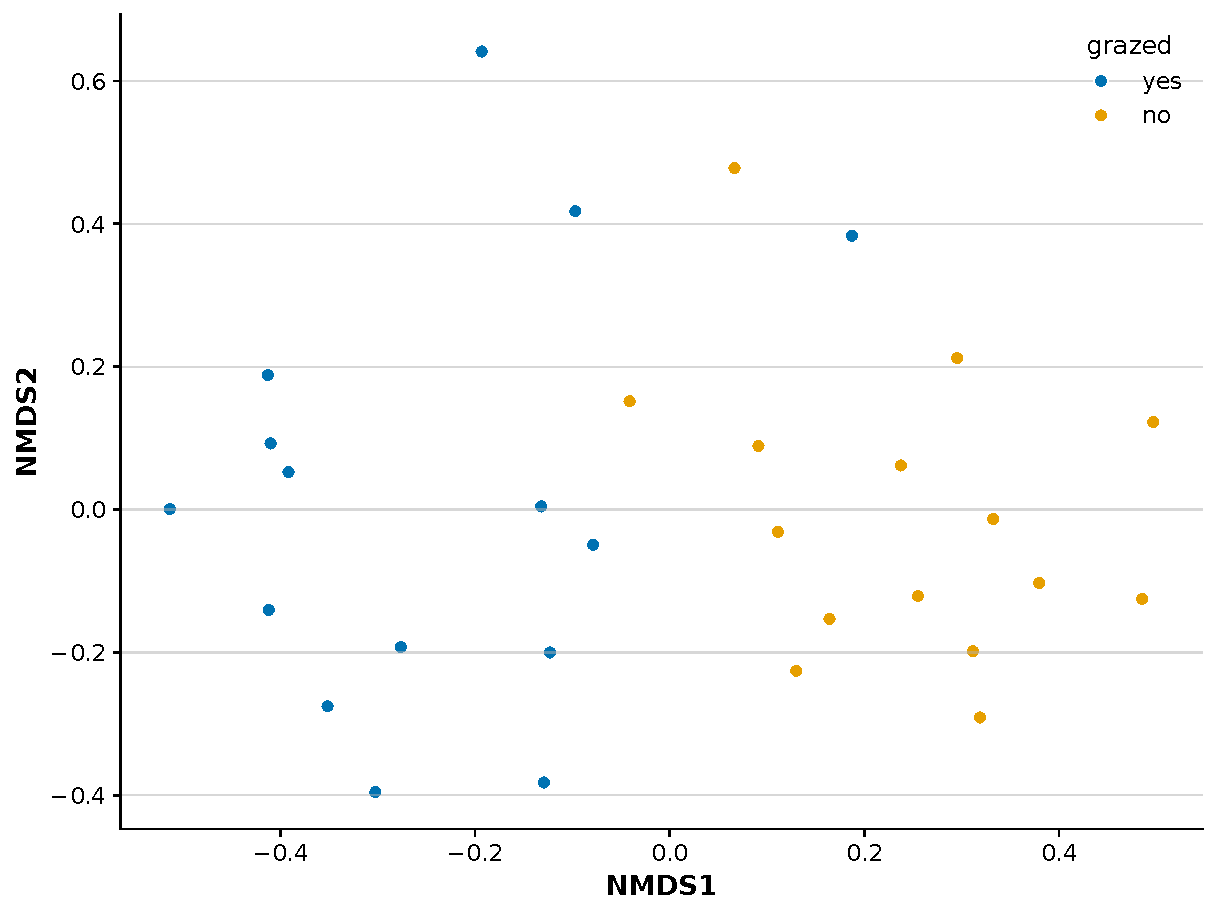
\includegraphics[width=0.72\textwidth,height=0.36\textheight,keepaspectratio]{figures/lesson17_example2_lesson17_nmds.pdf}
\captionof{figure}{Lesson 17, example 2: \code{lesson17\_\allowbreak{}nmds.\allowbreak{}png}.}
\end{minipage}\end{center}
\section*{Example 3}
Clustering finds groups of similar rows without being told the groups.
\begin{lstlisting}[style=py]
import simplydata as sdata
table = sdata.table(sdata.get_example("meadow"))
table.add_clusters(how_many=2)
table.count_rows(for_each_group_in="cluster", across="grazed")
\end{lstlisting}
\whateachline
\begin{lineexplain}
  \item[1] Load simplydata.
  \item[2] The meadow table.
  \item[3] k-means clustering: adds a column \code{\textquotedbl{}cluster\textquotedbl{}} with 1 or 2.
  \item[4] Did the clusters find the grazing? Cluster 1 is 14 grazed plots, cluster 2 is the 15 ungrazed plots and one grazed one.
\end{lineexplain}
\printedoutput{output/lesson17_example3.txt}
\begin{goodtoknow}
\begin{itemize}
  \item \code{same\_\allowbreak{}scale=True} (the normal choice for PCA and clusters) puts every column on the same scale first, so a column with big numbers does not drown the others.
  \item The signs and the rotation of PC and NMDS axes are arbitrary; only the distances between the dots mean something.
  \item Clarke's rule for NMDS stress: below 0.05 excellent, below 0.1 good, below 0.2 usable, above 0.2 hard to trust. Try \code{dimensions=3} if the stress is high.
  \item PERMANOVA can mistake a difference in spread for a difference in make-up, so \code{compare\_\allowbreak{}profiles\_\allowbreak{}of} also checks the spread of each group and says if it differs.
  \item Clusters always appear, even in data without groups: check them against what you know.
  \item \code{method=\textquotedbl{}hierarchical\textquotedbl{}} clusters step by step (Ward linkage) instead of k-means.
\end{itemize}
\end{goodtoknow}
\begin{tryit}
\begin{enumerate}
  \item Add principal components of \code{\textquotedbl{}hours\textquotedbl{}}, \code{\textquotedbl{}sleep\textquotedbl{}}, \code{\textquotedbl{}marks\textquotedbl{}} and \code{\textquotedbl{}days\_\allowbreak{}absent\textquotedbl{}} in \code{sdata.\allowbreak{}get\_\allowbreak{}example(\textquotedbl{}school\textquotedbl{})}. Which columns weigh most in PC1?
  \item Make an NMDS map of the meadow in 3 dimensions. Is the stress lower than in 2?
  \item Do the three fields differ in make-up? Use \code{compare\_\allowbreak{}profiles\_\allowbreak{}of} with \code{for\_\allowbreak{}each\_\allowbreak{}group\_\allowbreak{}in=\textquotedbl{}field\textquotedbl{}}.
  \item Cluster the meadow plots with \code{method=\textquotedbl{}hierarchical\textquotedbl{}}. Do the clusters match the grazing?
\end{enumerate}
Worked solutions: page~\pageref{solutions:17}, or type \code{sdata.\allowbreak{}show\_\allowbreak{}lesson(17,\allowbreak{} solutions=True)}.
\end{tryit}
\par\noindent{\small\sffamily\textbf{Words in this lesson:} \hyperref[word:table.add-principal-components]{\code{table.\allowbreak{}add\_\allowbreak{}principal\_\allowbreak{}components()}}, \hyperref[word:table.find-principal-components-of]{\code{table.\allowbreak{}find\_\allowbreak{}principal\_\allowbreak{}components\_\allowbreak{}of()}}, \hyperref[word:table.add-clusters]{\code{table.\allowbreak{}add\_\allowbreak{}clusters()}}, \hyperref[word:table.find-distances-between-rows]{\code{table.\allowbreak{}find\_\allowbreak{}distances\_\allowbreak{}between\_\allowbreak{}rows()}}, \hyperref[word:table.add-nmds]{\code{table.\allowbreak{}add\_\allowbreak{}nmds()}}, \hyperref[word:table.compare-profiles-of]{\code{table.\allowbreak{}compare\_\allowbreak{}profiles\_\allowbreak{}of()}}, \hyperref[word:draw-dots]{\code{chart.\allowbreak{}draw\_\allowbreak{}dots()}}.\par}

\chapter{Survival, and planning a study}\label{lesson:18}
\begin{learnbox}
\begin{itemize}
  \item how to draw survival curves (Kaplan-Meier) and compare them (log-rank test)
  \item how to explain the risk of an event from several columns (a Cox model)
  \item how many values a study needs, before you collect them (power analysis)
\end{itemize}
\end{learnbox}
\begin{needsr}The proportional-hazards check inside \code{explain\_\allowbreak{}survival()} (R survival::\code{cox.\allowbreak{}zph()}); the rest of the lesson needs no R. Without R that one check is left out with a note. The check and the other R words run R's own code, the same code R users run. Install it once: pip install \code{\textquotedbl{}simplydata[r]\textquotedbl{}}, then R from https://cran.r-project.org, then in R: \code{install.\allowbreak{}packages(c(\textquotedbl{}vegan\textquotedbl{},\allowbreak{} \textquotedbl{}survival\textquotedbl{},\allowbreak{} \textquotedbl{}mice\textquotedbl{},\allowbreak{} \textquotedbl{}emmeans\textquotedbl{}))}. Without R these words print a message that says what to install.\end{needsr}
\section*{Example 1}
In a trial, some patients are still alive when the follow-up ends. Survival words use their time too: they count as followed without the event (censored).
\begin{lstlisting}[style=py]
import simplydata as sdata
table = sdata.table(sdata.get_example("trial"))
table.find_survival_over_time(time="days", event="died", for_each_group_in="treatment")
chart = table.start_chart()
chart.draw_survival_curves(time="days", event="died", colour="treatment", with_confidence_band=True, with_at_risk_table=True)
chart.save("lesson18_survival.png")
\end{lstlisting}
\whateachline
\begin{lineexplain}
  \item[1] Load simplydata.
  \item[2] 120 patients, a new medicine or usual care, followed for up to 3 years.
  \item[3] The Kaplan-Meier estimate: the share still alive at each time, and the median time (706 days with the new medicine, 545 with usual care).
  \item[4] Start a chart.
  \item[5] Survival curves with their 95 \% bands, ticks where patients were censored, and the number still followed under the x-axis.
  \item[6] Save it.
\end{lineexplain}
\printedoutput{output/lesson18_example1.txt}
\begin{center}\begin{minipage}{\linewidth}\centering
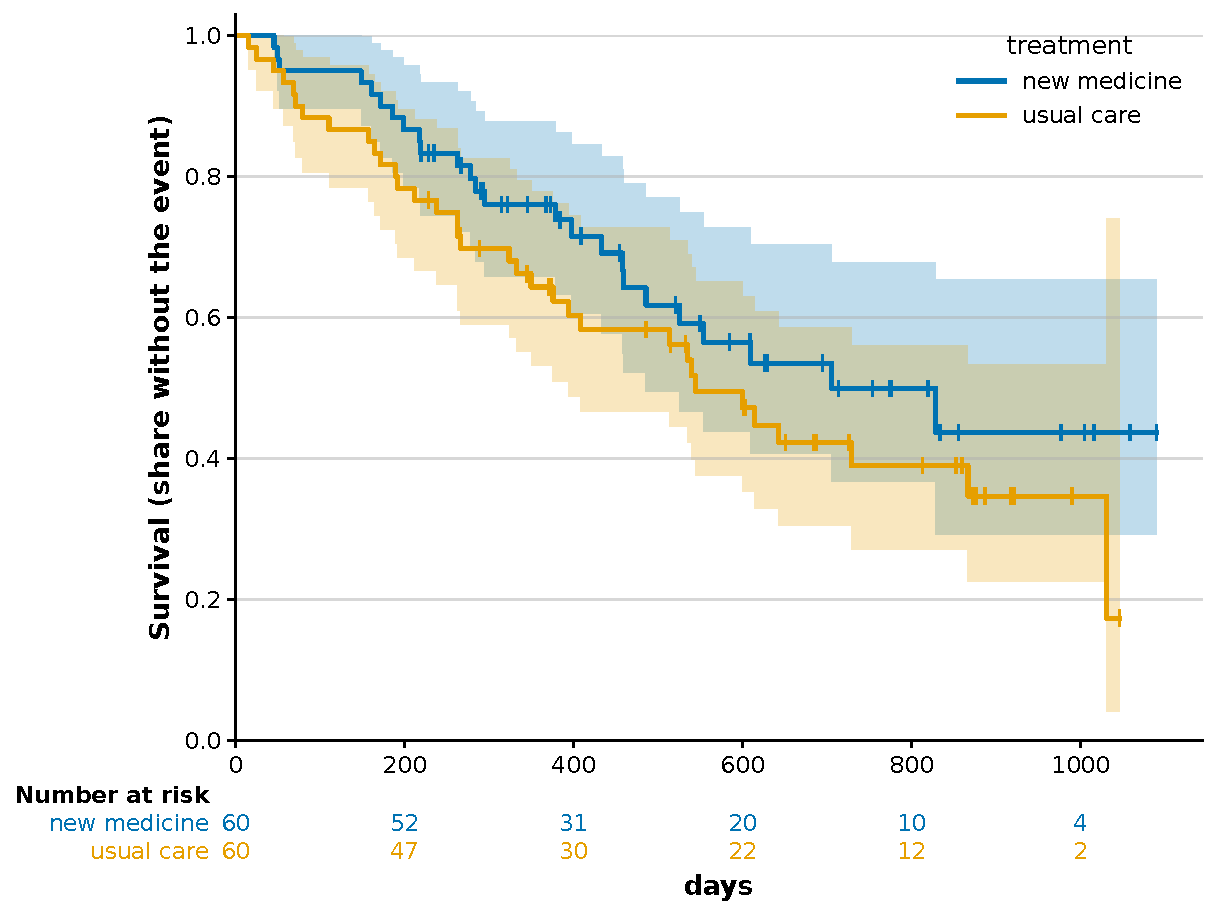
\includegraphics[width=0.72\textwidth,height=0.36\textheight,keepaspectratio]{figures/lesson18_example1_lesson18_survival.pdf}
\captionof{figure}{Lesson 18, example 1: \code{lesson18\_\allowbreak{}survival.\allowbreak{}png}.}
\end{minipage}\end{center}
\section*{Example 2}
Is the difference real? And what else changes the risk?
\begin{lstlisting}[style=py]
import simplydata as sdata
table = sdata.table(sdata.get_example("trial"))
table.compare_survival(time="days", event="died", for_each_group_in="treatment")
table.explain_survival(time="days", event="died", using=["treatment", "age"])
\end{lstlisting}
\whateachline
\begin{lineexplain}
  \item[1] Load simplydata.
  \item[2] The trial table.
  \item[3] The log-rank test compares the whole curves: here the data cannot tell (p = 0.22; differences this big would turn up in about 22 of 100 studies with truly alike groups).
  \item[4] A Cox model: each year of age raises the risk of dying at any moment by about 5 \% (hazard ratio 1.05), with the treatment held fixed.
\end{lineexplain}
\printedoutput{output/lesson18_example2.txt}
\section*{Example 3}
Was the trial big enough? Power analysis tells you how many values you need before you collect them.
\begin{lstlisting}[style=py]
import simplydata as sdata
sdata.find_how_many_needed(effect_size=0.5, power=0.8)
sdata.find_chance_of_finding(effect_size=0.5, values_per_group=20)
\end{lstlisting}
\whateachline
\begin{lineexplain}
  \item[1] Load simplydata.
  \item[2] To find a medium difference between two averages (half a standard deviation) with an 80 \% chance, you need 64 values in each group.
  \item[3] With only 20 values in each group, the chance to find it is just 34 \%.
\end{lineexplain}
\printedoutput{output/lesson18_example3.txt}
\begin{goodtoknow}
\begin{itemize}
  \item Never leave out the censored rows or count them as survivors: the survival words use the time they were followed, which is what makes these methods right.
  \item A hazard ratio above 1 means a higher risk of the event at any moment; 1 means no difference. The Cox model assumes the ratio stays the same over time, and simplydata checks this and says so if it does not.
  \item A study that is too small often finds nothing even when there is something to find. Plan the size before collecting data, not after.
  \item \code{effect\_\allowbreak{}size=} is Cohen's d for averages, f for 3 or more groups, w for counts and r for a correlation. You can also give \code{difference=} and \code{spread=} in your own units.
\end{itemize}
\end{goodtoknow}
\begin{tryit}
\begin{enumerate}
  \item Explain the risk of dying from \code{\textquotedbl{}age\textquotedbl{}} alone with \code{explain\_\allowbreak{}survival}.
  \item How many pairs does a before/after study need to find a small change (\code{effect\_\allowbreak{}size=0.\allowbreak{}3})?
  \item What is the chance to find a medium difference (\code{effect\_\allowbreak{}size=0.\allowbreak{}25}) between 3 groups with 30 values in each?
\end{enumerate}
Worked solutions: page~\pageref{solutions:18}, or type \code{sdata.\allowbreak{}show\_\allowbreak{}lesson(18,\allowbreak{} solutions=True)}.
\end{tryit}
\par\noindent{\small\sffamily\textbf{Words in this lesson:} \hyperref[word:table.find-survival-over-time]{\code{table.\allowbreak{}find\_\allowbreak{}survival\_\allowbreak{}over\_\allowbreak{}time()}}, \hyperref[word:draw-survival-curves]{\code{chart.\allowbreak{}draw\_\allowbreak{}survival\_\allowbreak{}curves()}}, \hyperref[word:table.compare-survival]{\code{table.\allowbreak{}compare\_\allowbreak{}survival()}}, \hyperref[word:table.explain-survival]{\code{table.\allowbreak{}explain\_\allowbreak{}survival()}}, \hyperref[word:sdata.find-how-many-needed]{\code{sdata.\allowbreak{}find\_\allowbreak{}how\_\allowbreak{}many\_\allowbreak{}needed()}}, \hyperref[word:sdata.find-chance-of-finding]{\code{sdata.\allowbreak{}find\_\allowbreak{}chance\_\allowbreak{}of\_\allowbreak{}finding()}}.\par}

\chapter{Fitting curves, finding the best value and solving}\label{lesson:19}
\begin{learnbox}
\begin{itemize}
  \item how to fit a straight line, a curve or any formula to your data, on a table and on a chart
  \item how to find where a formula is smallest or biggest
  \item how to solve an equation, also one made from a fitted formula
\end{itemize}
\end{learnbox}
\section*{Example 1}
Start with something you know: a straight line through the dots. \code{fit\_\allowbreak{}line}, \code{fit\_\allowbreak{}curve} and \code{fit\_\allowbreak{}formula} are the same words on a table (the numbers) and on a chart (the picture).
\begin{lstlisting}[style=py]
import simplydata as sdata
table = sdata.table(sdata.get_example("marks"))
table.fit_line(x="hours", y="marks")
table.fit_curve(x="hours", y="marks", of_degree=2)
chart = table.start_chart()
chart.draw_dots(x="hours", y="marks")
chart.fit_line()
chart.fit_curve(of_degree=2)
chart.save("lesson19_line_and_curve.png")
\end{lstlisting}
\whateachline
\begin{lineexplain}
  \item[1] Load simplydata.
  \item[2] The marks table: hours of study and marks.
  \item[3] The straight line: about 5.2 marks more for each hour of study, and R squared 0.69.
  \item[4] A curve with one bend (hours and hours**2). R squared only goes from 0.69 to 0.70, so the bend adds little: the straight line is enough here.
  \item[5] Start a chart of the same table.
  \item[6] The dots.
  \item[7] The same straight line, drawn.
  \item[8] And the curve, to see how close they are.
  \item[9] Save it.
\end{lineexplain}
\printedoutput{output/lesson19_example1.txt}
\begin{center}\begin{minipage}{\linewidth}\centering
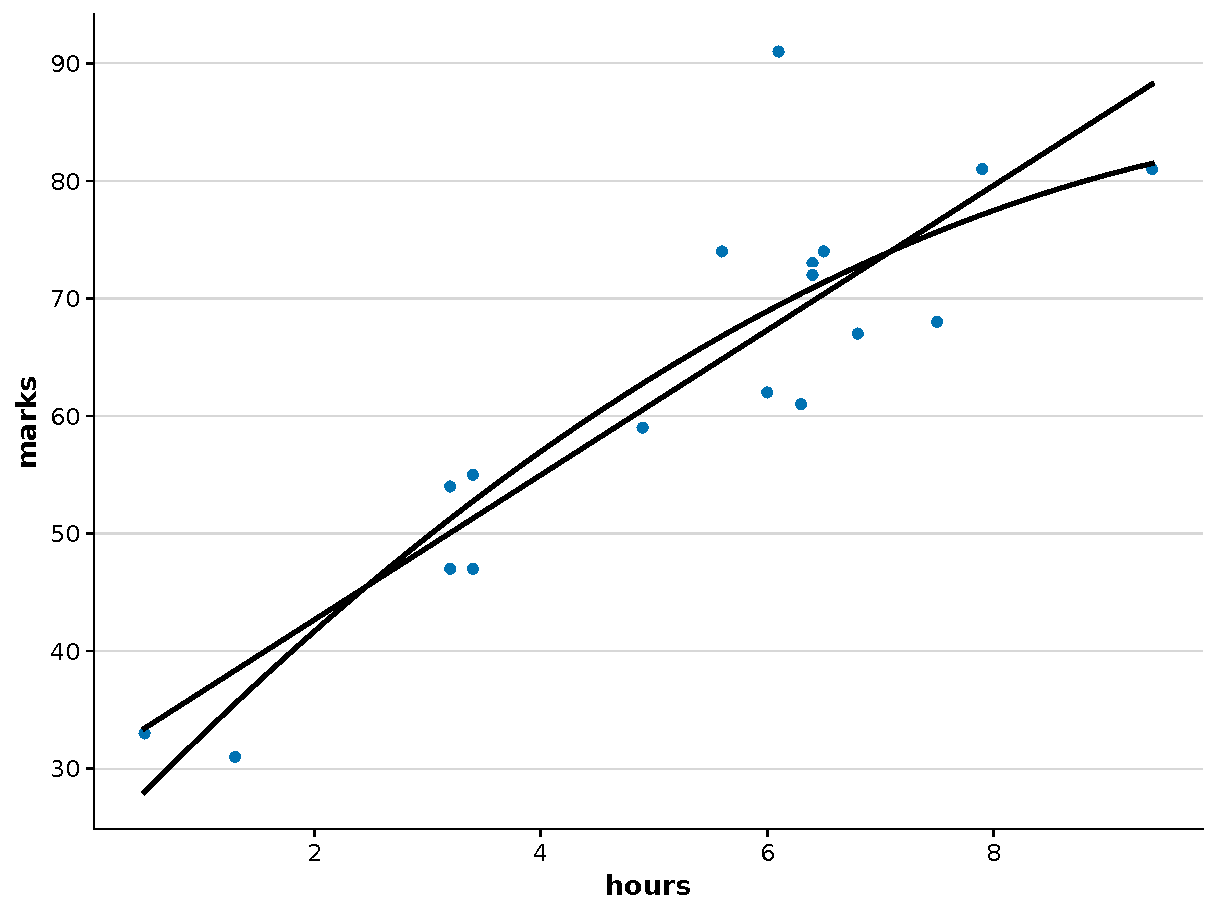
\includegraphics[width=0.72\textwidth,height=0.36\textheight,keepaspectratio]{figures/lesson19_example1_lesson19_line_and_curve.pdf}
\captionof{figure}{Lesson 19, example 1: \code{lesson19\_\allowbreak{}line\_\allowbreak{}and\_\allowbreak{}curve.\allowbreak{}png}.}
\end{minipage}\end{center}
\section*{Example 2}
A research question: how fast does each country grow? Growth by a fixed share each year is the formula population = a * \code{exp(b * (year - 2000))}. Names that are columns (population, year) are data; the other names (a, b) are the values to find.
\begin{lstlisting}[style=py]
import simplydata as sdata
table = sdata.table(sdata.get_example("growth"))
table.fit_formula("population = a * exp(b * (year - 2000))", for_each_group_in="country")
chart = table.start_chart()
chart.draw_dots(x="year", y="population", colour="country")
chart.fit_formula("population = a * exp(b * (year - 2000))")
chart.save("lesson19_growth.png")
\end{lstlisting}
\whateachline
\begin{lineexplain}
  \item[1] Load simplydata.
  \item[2] Four countries, every two years.
  \item[3] One fit for each country, by nonlinear least squares (as R \code{nls()}). a is the population in 2000 and b the growth rate: Cherria grows fastest, b = 0.0443, about 4.5 \% a year.
  \item[4] Start a chart.
  \item[5] The data, one colour per country.
  \item[6] The fitted curve of each country, with the same values as the table word.
  \item[7] Save it.
\end{lineexplain}
\printedoutput{output/lesson19_example2.txt}
\begin{center}\begin{minipage}{\linewidth}\centering
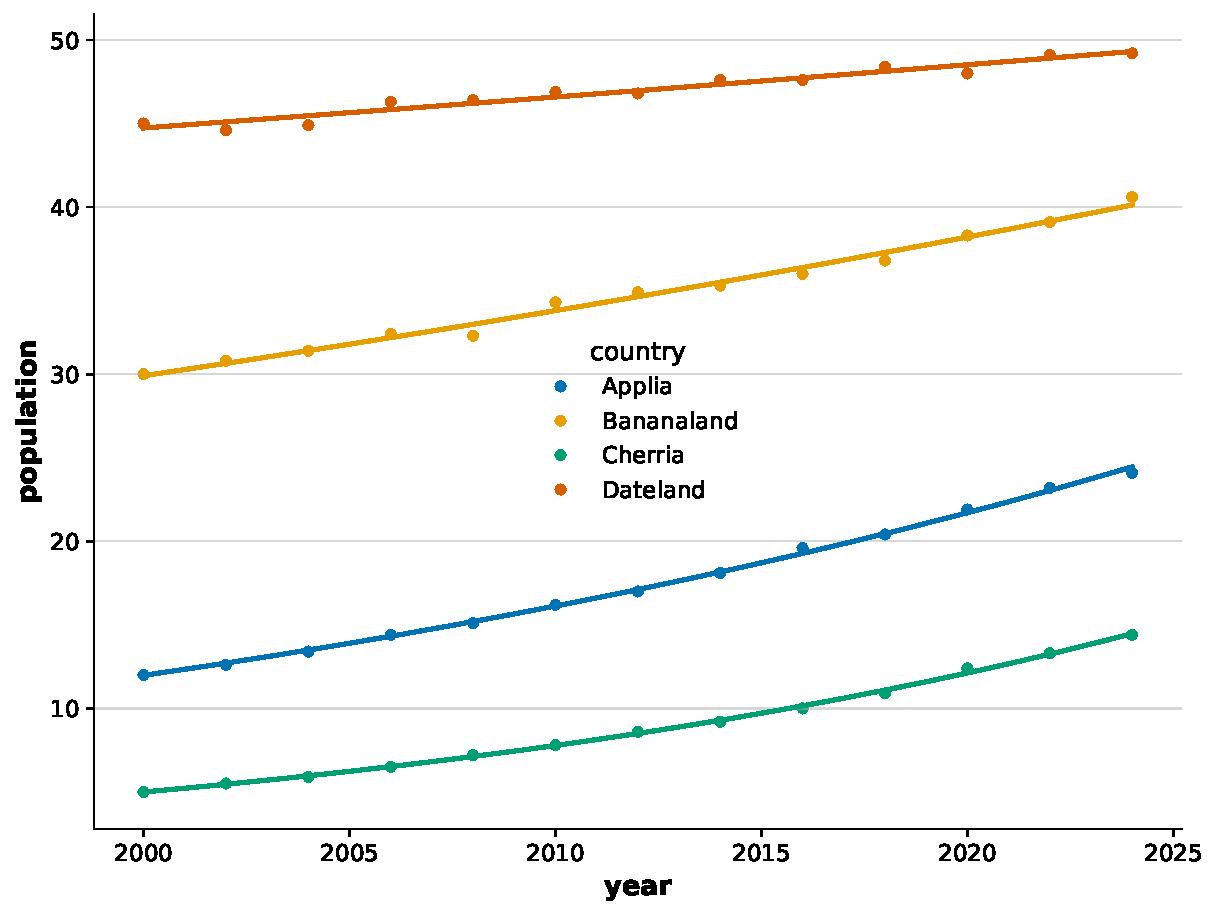
\includegraphics[width=0.72\textwidth,height=0.36\textheight,keepaspectratio]{figures/lesson19_example2_lesson19_growth.pdf}
\captionof{figure}{Lesson 19, example 2: \code{lesson19\_\allowbreak{}growth.\allowbreak{}png}.}
\end{minipage}\end{center}
\section*{Example 3}
Finding and solving: \code{sdata.\allowbreak{}find\_\allowbreak{}where\_\allowbreak{}smallest}, \code{sdata.\allowbreak{}find\_\allowbreak{}where\_\allowbreak{}biggest} and \code{sdata.\allowbreak{}solve} work on a formula. The names in it are what to find; \code{between=} says where to look.
\begin{lstlisting}[style=py]
import simplydata as sdata
sdata.find_where_smallest("x**2 - 4*x + 1", between=[0, 5])
sdata.find_where_biggest("3*x + 2*y", rules=["x + y <= 4", "x + 3*y <= 6", "x >= 0", "y >= 0"])
sdata.solve("x**3 - 2*x = 5", between=[0, 3])
table = sdata.table(sdata.get_example("growth"))
table.keep_rows_where("country", is_equal_to="Applia")
fit = table.fit_formula("population = a * exp(b * (year - 2000))")
sdata.solve("a * exp(b * (year - 2000)) = 20", between=[2000, 2050], known=fit)
\end{lstlisting}
\whateachline
\begin{lineexplain}
  \item[1] Load simplydata.
  \item[2] The smallest value is -3, at x = 2. The method and its R name are printed (R \code{optimize()}).
  \item[3] The biggest value under rules: 12, at x = 4 and y = 0. Everything is a straight line, so simplydata uses linear programming and says which rules are reached exactly.
  \item[4] The value of x that makes both sides equal: 2.09455. Every solution in the range is found.
  \item[5] Back to the growth table.
  \item[6] Keep one country.
  \item[7] Fit the growth formula and keep the result, a one-row table with a and b.
  \item[8] \code{known=fit} puts the fitted a and b into the equation: Applia reaches 20 million in about 2017 (year = 2017.24). A fitted curve answers questions, not only draws a line.
\end{lineexplain}
\printedoutput{output/lesson19_example3.txt}
\begin{goodtoknow}
\begin{itemize}
  \item Fitting is the same idea every time: a line, a curve or a formula is moved until it is as close to the points as it can be (least squares). The printed sentence says how sure each value is (its 95 \% confidence interval).
  \item A curve with a high \code{of\_\allowbreak{}degree=} can wiggle through every point and still say nothing true. Choose the simplest line or formula that follows the data, and a formula whose values mean something (here b is a growth rate).
  \item If a formula fit fails, give start values near the answer: \code{start=}\{\code{\textquotedbl{}a\textquotedbl{}}: 10, \code{\textquotedbl{}b\textquotedbl{}}: 0.03\}.
  \item \code{sdata.\allowbreak{}find\_\allowbreak{}where\_\allowbreak{}smallest} with \code{between=} finds one lowest point; when the curve has several dips it says so, and \code{search=\textquotedbl{}whole range\textquotedbl{}} looks everywhere. solve with \code{between=} finds every crossing.
  \item Names from other tools point to these words: minimize, optimise and argmin to \code{find\_\allowbreak{}where\_\allowbreak{}smallest}, fsolve, brentq and uniroot to solve, \code{curve\_\allowbreak{}fit} and nls to \code{fit\_\allowbreak{}formula}, polyfit to \code{fit\_\allowbreak{}curve}.
\end{itemize}
\end{goodtoknow}
\begin{tryit}
\begin{enumerate}
  \item Fit a curve of degree 3 to \code{\textquotedbl{}marks\textquotedbl{}} against \code{\textquotedbl{}hours\textquotedbl{}}. Does R squared go up much from the straight line?
  \item With the weather table, keep the city Sunnyvale and fit \code{\textquotedbl{}temperature = a + b * cos(2 * pi * (month\_\allowbreak{}number - c) / 12)\textquotedbl{}} with \code{start=}\{\code{\textquotedbl{}a\textquotedbl{}}: 15, \code{\textquotedbl{}b\textquotedbl{}}: 8, \code{\textquotedbl{}c\textquotedbl{}}: 7\}. In which month is it warmest (c)?
  \item Try to remember without looking back: which word finds where a formula is biggest, and which word finds where the two sides of an equation are equal? Use them on \code{\textquotedbl{}x * (10 - x)\textquotedbl{}} between 0 and 10, and on \code{\textquotedbl{}x**2 = 2\textquotedbl{}} between 0 and 2.
\end{enumerate}
Worked solutions: page~\pageref{solutions:19}, or type \code{sdata.\allowbreak{}show\_\allowbreak{}lesson(19,\allowbreak{} solutions=True)}.
\end{tryit}
\par\noindent{\small\sffamily\textbf{Words in this lesson:} \hyperref[word:table.fit-line]{\code{table.\allowbreak{}fit\_\allowbreak{}line()}}, \hyperref[word:table.fit-curve]{\code{table.\allowbreak{}fit\_\allowbreak{}curve()}}, \hyperref[word:table.fit-formula]{\code{table.\allowbreak{}fit\_\allowbreak{}formula()}}, \hyperref[word:fit-line]{\code{chart.\allowbreak{}fit\_\allowbreak{}line()}}, \hyperref[word:fit-curve]{\code{chart.\allowbreak{}fit\_\allowbreak{}curve()}}, \hyperref[word:fit-formula]{\code{chart.\allowbreak{}fit\_\allowbreak{}formula()}}, \hyperref[word:sdata.find-where-smallest]{\code{sdata.\allowbreak{}find\_\allowbreak{}where\_\allowbreak{}smallest()}}, \hyperref[word:sdata.find-where-biggest]{\code{sdata.\allowbreak{}find\_\allowbreak{}where\_\allowbreak{}biggest()}}, \hyperref[word:sdata.solve]{\code{sdata.\allowbreak{}solve()}}.\par}

\chapter{Distributions, chances and values between points}\label{lesson:20}
\begin{learnbox}
\begin{itemize}
  \item how to ask a distribution for chances, percentiles and cut-offs
  \item how to find which distribution fits your data, and check it
  \item how to estimate values between the points you measured
\end{itemize}
\end{learnbox}
\section*{Example 1}
A distribution says how likely each value is. Start with the bell curve (normal): marks with an average of 50 and a standard deviation of 10.
\begin{lstlisting}[style=py]
import simplydata as sdata
dist = sdata.distribution("normal", average=50, standard_deviation=10)
dist.find_chance_that_value(is_above=80)
dist.find_chance_that_value(is_between=[40, 60])
dist.find_percentile(95)
dist.find_cut_off(with_chance_above=0.025)
chart = dist.draw_chart()
chart.save("lesson20_normal.png")
\end{lstlisting}
\whateachline
\begin{lineexplain}
  \item[1] Load simplydata.
  \item[2] Make the distribution. R's names (\code{mean=}, \code{sd=}) work too.
  \item[3] The chance of a mark above 80: 0.135 \%. The R code that gives the same answer is printed too: \code{pnorm(80,\allowbreak{} .\allowbreak{}.\allowbreak{}.\allowbreak{})}.
  \item[4] 68.3 \%: about two in three are within one standard deviation of the average.
  \item[5] 95 \% of marks are below 66.4.
  \item[6] The cut-off with a 2.5 \% chance above it: 69.6. Tests use such cut-offs (critical values).
  \item[7] A chart of the bell curve.
  \item[8] Save it.
\end{lineexplain}
\printedoutput{output/lesson20_example1.txt}
\begin{center}\begin{minipage}{\linewidth}\centering
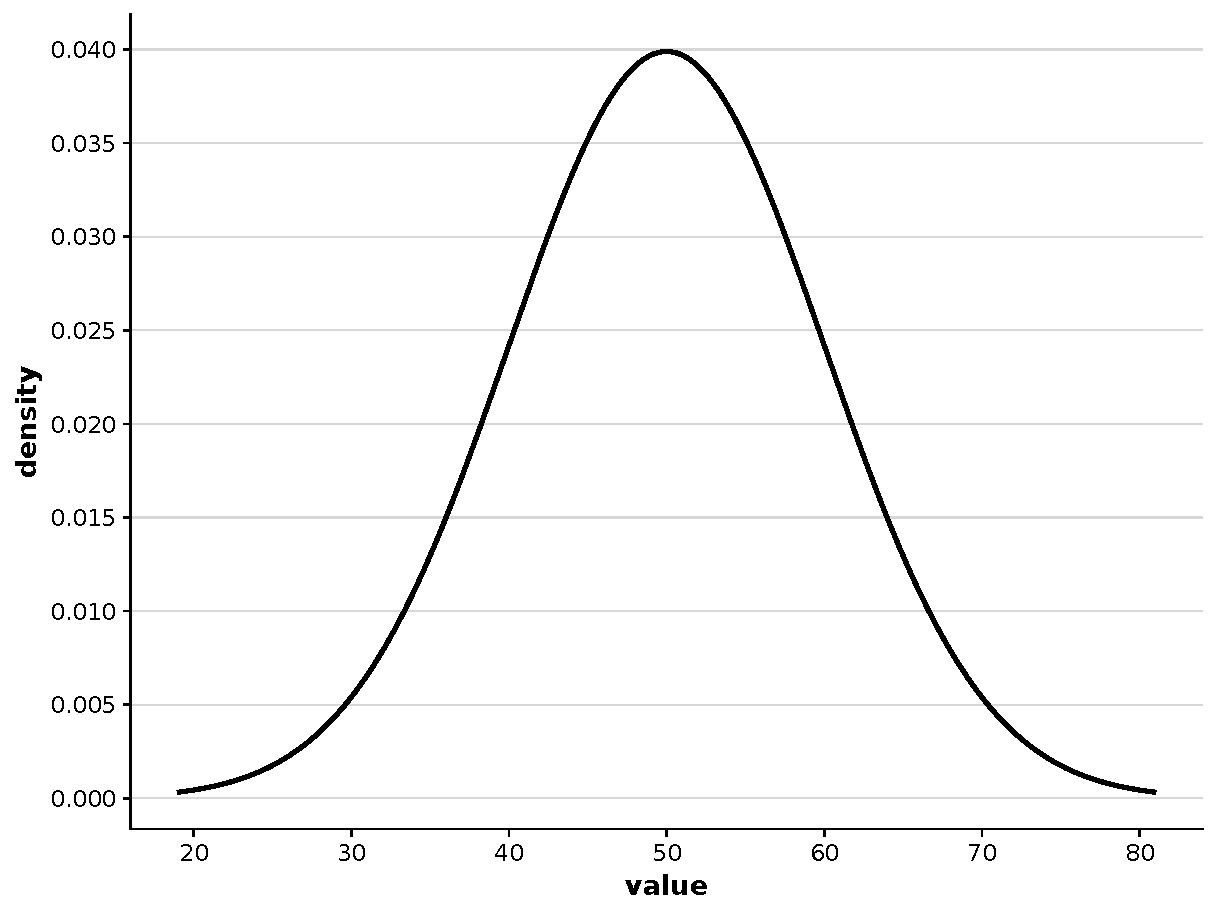
\includegraphics[width=0.72\textwidth,height=0.36\textheight,keepaspectratio]{figures/lesson20_example1_lesson20_normal.pdf}
\captionof{figure}{Lesson 20, example 1: \code{lesson20\_\allowbreak{}normal.\allowbreak{}png}.}
\end{minipage}\end{center}
\section*{Example 2}
A research question: pupils' days absent are counts (0, 1, 2 ...). Do they vary as a Poisson distribution expects, or more? The words that fit are \code{fit\_\allowbreak{}distribution\_\allowbreak{}to} and \code{compare\_\allowbreak{}distributions\_\allowbreak{}for}.
\begin{lstlisting}[style=py]
import simplydata as sdata
table = sdata.table(sdata.get_example("school"))
table.compare_distributions_for("days_absent", distributions=("poisson", "negative binomial"))
fit = table.fit_distribution_to("days_absent", "negative binomial")
fit.find_chance_that_value(is_at_least=10)
chart = table.start_chart()
chart.draw_histogram(x="days_absent", show="density")
chart.fit_distribution("negative binomial")
chart.save("lesson20_absent.png")
\end{lstlisting}
\whateachline
\begin{lineexplain}
  \item[1] Load simplydata.
  \item[2] 180 pupils and their days absent.
  \item[3] Both are fitted by maximum likelihood and ranked by AIC: the negative binomial wins by 7, so the counts vary more than Poisson allows.
  \item[4] Fit it and keep the fitted distribution.
  \item[5] The chance a pupil misses 10 days or more: 0.66 \%.
  \item[6] Start a chart.
  \item[7] The counts, as shares.
  \item[8] The fitted chance of each count, on top.
  \item[9] Save it.
\end{lineexplain}
\printedoutput{output/lesson20_example2.txt}
\begin{center}\begin{minipage}{\linewidth}\centering
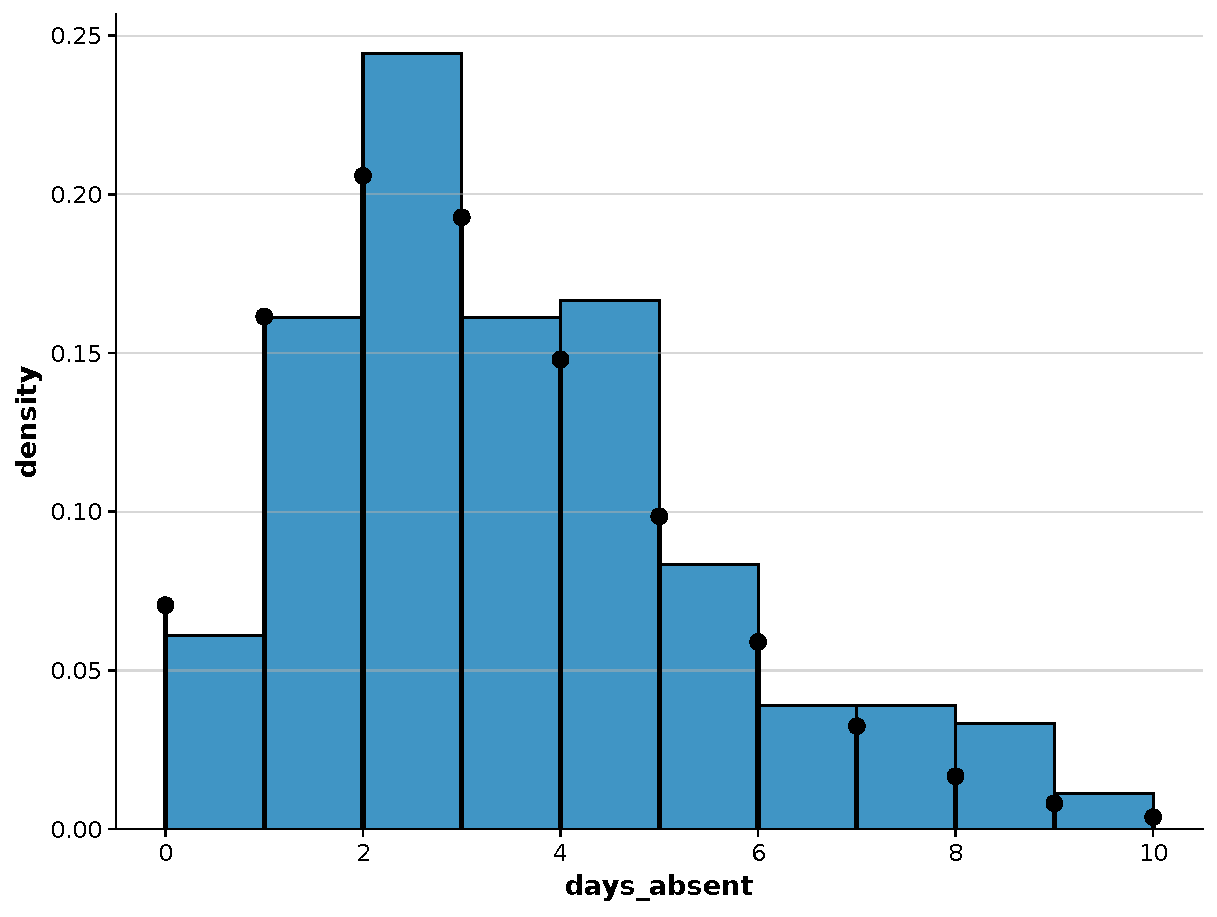
\includegraphics[width=0.72\textwidth,height=0.36\textheight,keepaspectratio]{figures/lesson20_example2_lesson20_absent.pdf}
\captionof{figure}{Lesson 20, example 2: \code{lesson20\_\allowbreak{}absent.\allowbreak{}png}.}
\end{minipage}\end{center}
\section*{Example 3}
Values between points: you measured every two years, but you need 2001. \code{values\_\allowbreak{}at} joins the dots (straight lines, or a smooth curve) and reads off the value; \code{make\_\allowbreak{}map\_\allowbreak{}of} does it across a whole map.
\begin{lstlisting}[style=py]
import simplydata as sdata
table = sdata.table(sdata.get_example("growth"))
estimates = table.values_at("population", at={"year": [2001, 2011]}, for_each_group_in="country")
estimates.show()
island = sdata.table(sdata.get_example("island"))
heights = island.make_map_of("height", across=["east", "north"], steps=60, joined_by="smooth surface")
chart = heights.start_chart()
chart.draw_contour(x="east", y="north", z="height")
chart.save("lesson20_map.png")
\end{lstlisting}
\whateachline
\begin{lineexplain}
  \item[1] Load simplydata.
  \item[2] Population every two years.
  \item[3] Straight lines between the known points (linear interpolation, as R \code{approx()}), for each country.
  \item[4] A new table with the estimates.
  \item[5] Heights measured on a 15 x 15 grid.
  \item[6] A finer 60 x 60 map, with a smooth surface through every point (a thin-plate spline).
  \item[7] A chart of the new map.
  \item[8] Its contour map.
  \item[9] Save it.
\end{lineexplain}
\printedoutput{output/lesson20_example3.txt}
\begin{center}\begin{minipage}{\linewidth}\centering
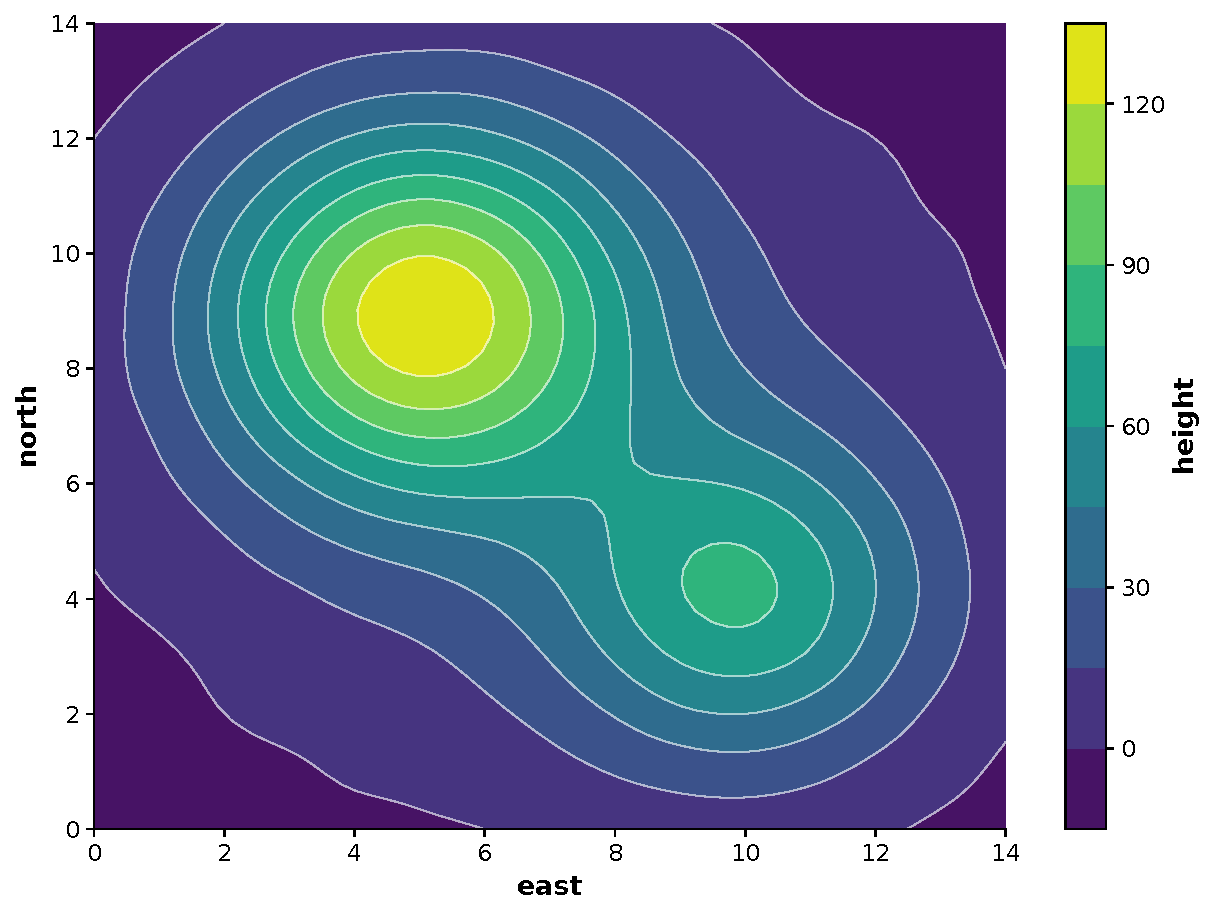
\includegraphics[width=0.72\textwidth,height=0.36\textheight,keepaspectratio]{figures/lesson20_example3_lesson20_map.pdf}
\captionof{figure}{Lesson 20, example 3: \code{lesson20\_\allowbreak{}map.\allowbreak{}png}.}
\end{minipage}\end{center}
\begin{goodtoknow}
\begin{itemize}
  \item \code{find\_\allowbreak{}chance\_\allowbreak{}that\_\allowbreak{}value()} gives back a share from 0 to 1 and prints it as a percent. \code{is\_\allowbreak{}above=} and \code{is\_\allowbreak{}below=} leave the value itself out, \code{is\_\allowbreak{}at\_\allowbreak{}least=} and \code{is\_\allowbreak{}at\_\allowbreak{}most=} keep it in, as in \code{keep\_\allowbreak{}rows\_\allowbreak{}where}. For counts that matters: \code{is\_\allowbreak{}at\_\allowbreak{}most=3} means 3 or fewer.
  \item \code{find\_\allowbreak{}density\_\allowbreak{}at()} is the height of the curve, not a chance: a chance is an area under the curve, so ask \code{find\_\allowbreak{}chance\_\allowbreak{}that\_\allowbreak{}value(is\_\allowbreak{}between=[.\allowbreak{}.\allowbreak{}.\allowbreak{}])}.
  \item A fitted distribution is only as good as its fit. Compare a few with \code{compare\_\allowbreak{}distributions\_\allowbreak{}for}, and test the shape with \code{table.\allowbreak{}compare\_\allowbreak{}shape\_\allowbreak{}to(\textquotedbl{}column\textquotedbl{},\allowbreak{} \textquotedbl{}gamma\textquotedbl{})}.
  \item Values between points are estimates. Straight lines are the safe choice; a smooth curve can swing above or below the points (\code{joined\_\allowbreak{}by=\textquotedbl{}curve without overshoot\textquotedbl{}} never does). Outside the measured range the cells stay empty unless you ask for \code{outside=}.
  \item Names from other tools point to these words: pnorm and cdf to chance, qnorm and ppf to percentile, dnorm and pdf to \code{find\_\allowbreak{}density\_\allowbreak{}at}, interpolate and approx to \code{values\_\allowbreak{}at}.
\end{itemize}
\end{goodtoknow}
\begin{tryit}
\begin{enumerate}
  \item Ten coins are thrown. With \code{sdata.\allowbreak{}distribution(\textquotedbl{}binomial\textquotedbl{},\allowbreak{} tries=10,\allowbreak{} chance=0.\allowbreak{}5)}, what is the chance of 8 heads or more?
  \item Which fits the daily \code{\textquotedbl{}sales\textquotedbl{}} of the shop table best: normal, lognormal, gamma or weibull? Then check the best one with \code{compare\_\allowbreak{}shape\_\allowbreak{}to}.
  \item Try to remember without looking back: which word estimates a value between the points you measured? Use it to estimate the temperature of each city at \code{month\_\allowbreak{}number} 6.5, joined by a smooth curve.
\end{enumerate}
Worked solutions: page~\pageref{solutions:20}, or type \code{sdata.\allowbreak{}show\_\allowbreak{}lesson(20,\allowbreak{} solutions=True)}.
\end{tryit}
\par\noindent{\small\sffamily\textbf{Words in this lesson:} \hyperref[word:sdata.distribution]{\code{sdata.\allowbreak{}distribution()}}, \hyperref[word:dist.find-chance-that-value]{\code{dist.\allowbreak{}find\_\allowbreak{}chance\_\allowbreak{}that\_\allowbreak{}value()}}, \hyperref[word:dist.find-percentile]{\code{dist.\allowbreak{}find\_\allowbreak{}percentile()}}, \hyperref[word:dist.find-cut-off]{\code{dist.\allowbreak{}find\_\allowbreak{}cut\_\allowbreak{}off()}}, \hyperref[word:dist.draw-chart]{\code{dist.\allowbreak{}draw\_\allowbreak{}chart()}}, \hyperref[word:table.compare-distributions-for]{\code{table.\allowbreak{}compare\_\allowbreak{}distributions\_\allowbreak{}for()}}, \hyperref[word:table.fit-distribution-to]{\code{table.\allowbreak{}fit\_\allowbreak{}distribution\_\allowbreak{}to()}}, \hyperref[word:fit-distribution]{\code{chart.\allowbreak{}fit\_\allowbreak{}distribution()}}, \hyperref[word:table.values-at]{\code{table.\allowbreak{}values\_\allowbreak{}at()}}, \hyperref[word:table.make-map-of]{\code{table.\allowbreak{}make\_\allowbreak{}map\_\allowbreak{}of()}}, \hyperref[word:draw-curve]{\code{chart.\allowbreak{}draw\_\allowbreak{}curve()}}.\par}

\chapter{Working with a model: check it, compare it, predict with it}\label{lesson:21}
\begin{learnbox}
\begin{itemize}
  \item how to check a model from \code{explain()} with four pictures (\code{check\_\allowbreak{}model\_\allowbreak{}of})
  \item how to find the rows that pull a model the most (\code{show\_\allowbreak{}rows\_\allowbreak{}that\_\allowbreak{}pull\_\allowbreak{}model})
  \item how to ask whether a column helps a model (\code{compare\_\allowbreak{}models})
  \item how sure a prediction is, for the average and for one new row (\code{add\_\allowbreak{}predicted\_\allowbreak{}column} with \code{interval=95})
  \item if you have R: the average of each group once the other columns are allowed for (\code{find\_\allowbreak{}model\_\allowbreak{}averages\_\allowbreak{}of})
\end{itemize}
\end{learnbox}
\begin{needsr}Only example 5, which you may leave out, needs R: \code{find\_\allowbreak{}model\_\allowbreak{}averages\_\allowbreak{}of()} (R emmeans). The rest of the lesson needs no R. \code{find\_\allowbreak{}model\_\allowbreak{}averages\_\allowbreak{}of()} and the other R words run R's own code, the same code R users run. Install it once: pip install \code{\textquotedbl{}simplydata[r]\textquotedbl{}}, then R from https://cran.r-project.org, then in R: \code{install.\allowbreak{}packages(c(\textquotedbl{}vegan\textquotedbl{},\allowbreak{} \textquotedbl{}survival\textquotedbl{},\allowbreak{} \textquotedbl{}mice\textquotedbl{},\allowbreak{} \textquotedbl{}emmeans\textquotedbl{}))}. Without R these words print a message that says what to install.\end{needsr}
\section*{Example 1}
\code{explain()} gives the effects, but they can only be trusted if the model suits the data. \code{check\_\allowbreak{}model\_\allowbreak{}of} draws the four pictures R users look at first.
\begin{lstlisting}[style=py]
import simplydata as sdata
table = sdata.table(sdata.get_example("school"))
table.explain("marks", using=["hours", "breakfast"])
page = table.check_model_of("marks", using=["hours", "breakfast"])
page.save("lesson21_checks.png")
\end{lstlisting}
\whateachline
\begin{lineexplain}
  \item[1] Load simplydata.
  \item[2] The pupils of lesson 16.
  \item[3] The model to check: 2.82 more marks for each hour of study and 3.21 more with breakfast. The line under the effects says how well it fits: AIC 1292 and BIC 1305, numbers that only mean something when you compare two models.
  \item[4] Four pictures of the same model. Here the residuals lie in an even band around 0, the dots follow the Q-Q line, the scale-location line is flat, and the dashed Cook's distance lines lie outside the leverage picture: no row comes near them. The variance inflation factors are 1.00: hours and breakfast are not linked.
  \item[5] Save the page of pictures.
\end{lineexplain}
\printedoutput{output/lesson21_example1.txt}
\begin{center}\begin{minipage}{\linewidth}\centering
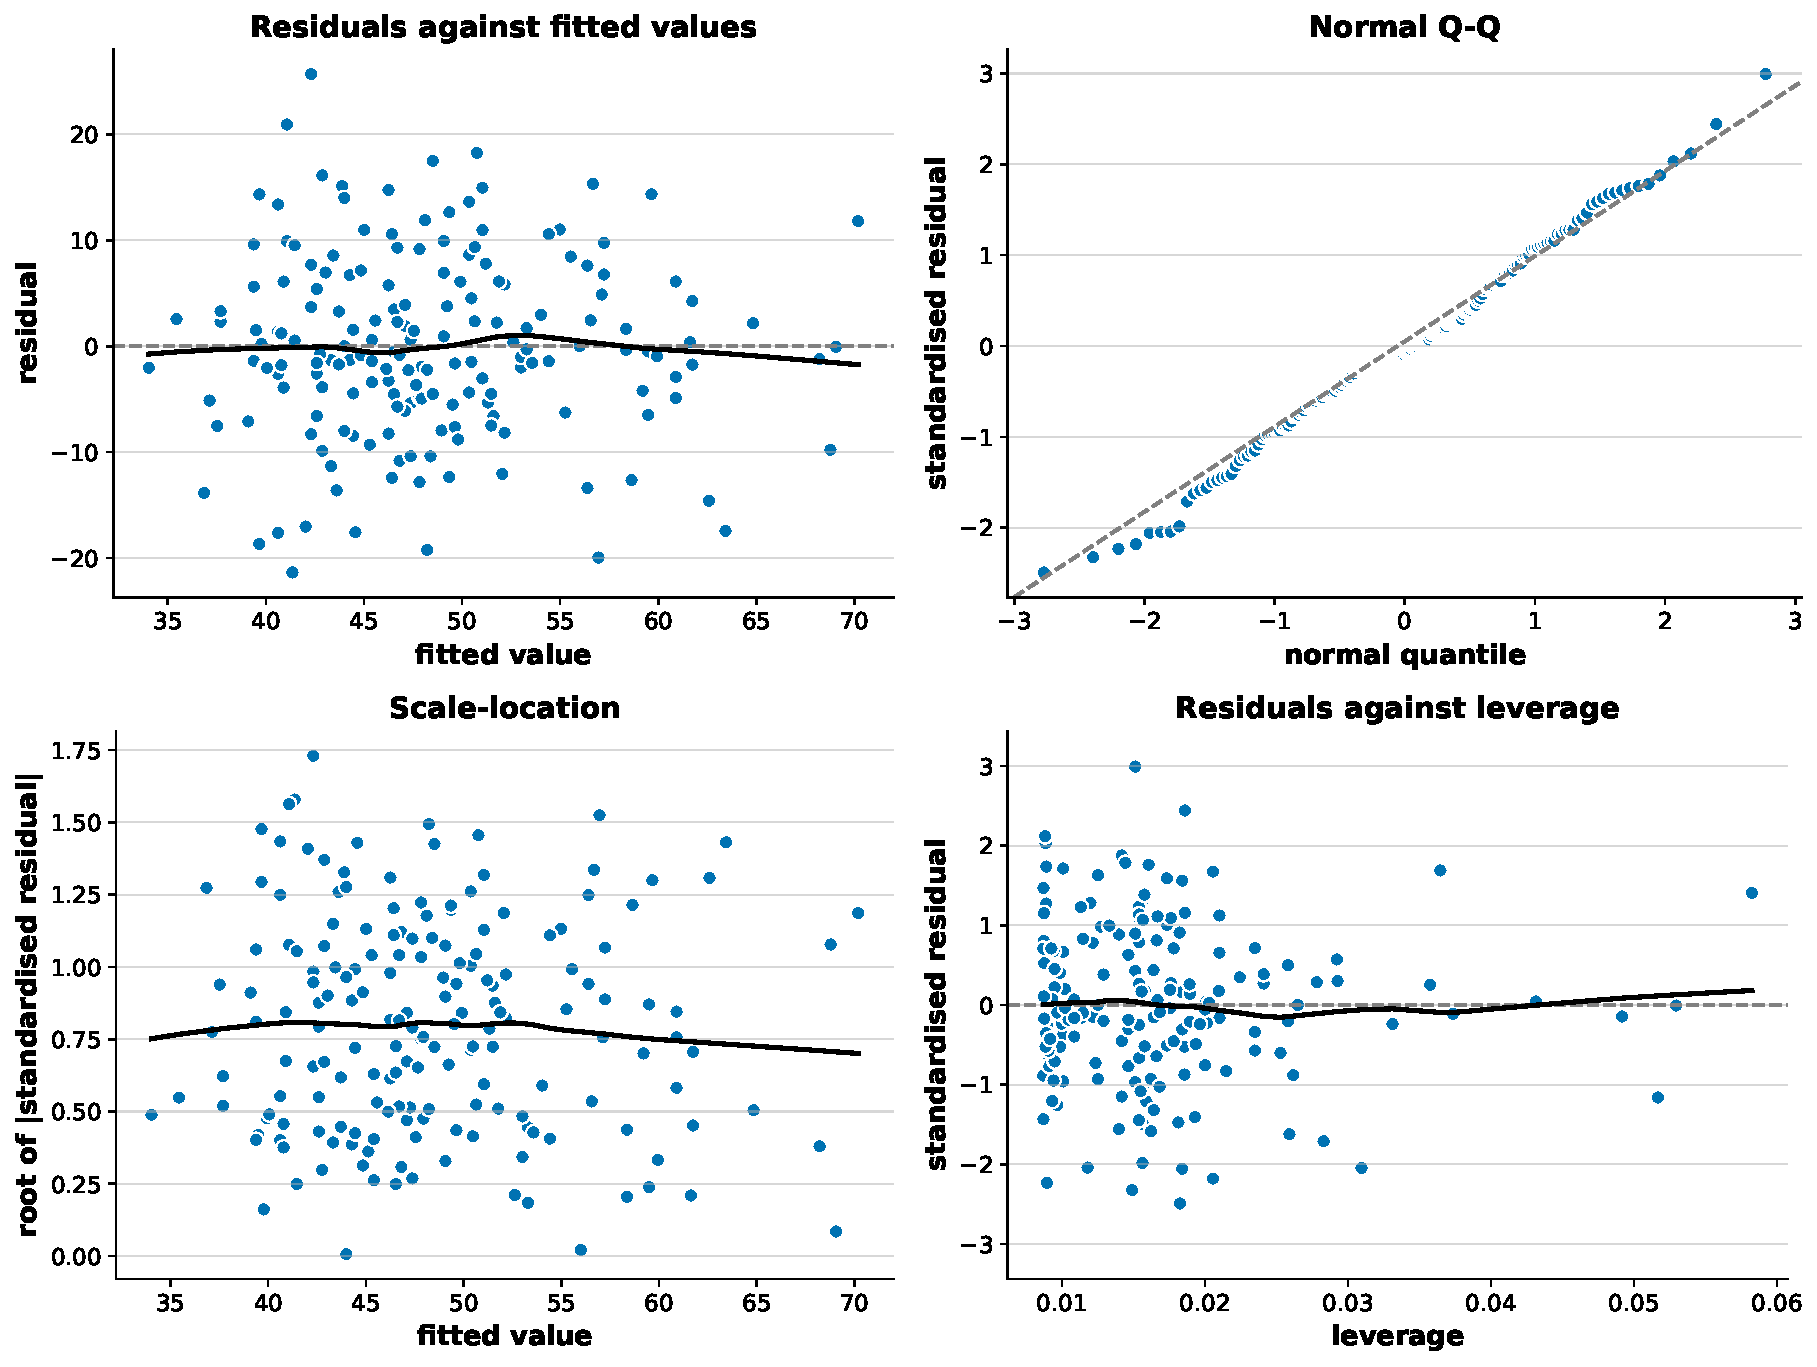
\includegraphics[width=0.72\textwidth,height=0.36\textheight,keepaspectratio]{figures/lesson21_example1_lesson21_checks.pdf}
\captionof{figure}{Lesson 21, example 1: \code{lesson21\_\allowbreak{}checks.\allowbreak{}png}.}
\end{minipage}\end{center}
\section*{Example 2}
Some rows pull a model more than others. \code{show\_\allowbreak{}rows\_\allowbreak{}that\_\allowbreak{}pull\_\allowbreak{}model} lists them, the strongest first, so you can look at them before you trust the model.
\begin{lstlisting}[style=py]
import simplydata as sdata
table = sdata.table(sdata.get_example("school"))
table.show_rows_that_pull_model("marks", using=["hours", "breakfast"])
\end{lstlisting}
\whateachline
\begin{lineexplain}
  \item[1] Load simplydata.
  \item[2] The school table.
  \item[3] 12 of the 180 rows have a Cook's distance above the rule of thumb 4 / 180 = 0.0222. The biggest, row 48 (0.0459), is far below 0.5, where the pictures draw the first dashed line: no row pulls strongly. The table itself does not change.
\end{lineexplain}
\printedoutput{output/lesson21_example2.txt}
\section*{Example 3}
Does a column help? \code{compare\_\allowbreak{}models} fits the model with and without it, on the same rows, and tests the difference.
\begin{lstlisting}[style=py]
import simplydata as sdata
table = sdata.table(sdata.get_example("school"))
table.compare_models("marks", using=["hours"], against=["hours", "breakfast"])
\end{lstlisting}
\whateachline
\begin{lineexplain}
  \item[1] Load simplydata.
  \item[2] The school table.
  \item[3] Does breakfast help a model that already has hours? The F test: about 2 of 100 studies would show this much if breakfast truly did not help (p = 0.018), and the AIC is 3.72 lower with breakfast: keep it.
\end{lineexplain}
\printedoutput{output/lesson21_example3.txt}
\section*{Example 4}
A prediction is never exact. \code{interval=95} says how sure the model is about the average; \code{for\_\allowbreak{}new\_\allowbreak{}rows=True} says where one new pupil would fall, which is much wider.
\begin{lstlisting}[style=py]
import simplydata as sdata
table = sdata.table(sdata.get_example("school"))
table.add_predicted_column("marks", using=["hours", "breakfast"], name="average", interval=95)
table.add_predicted_column("marks", using=["hours", "breakfast"], name="new pupil", interval=95, for_new_rows=True)
table.keep_columns(contains="95 %")
table.show(rows=3)
\end{lstlisting}
\whateachline
\begin{lineexplain}
  \item[1] Load simplydata.
  \item[2] The school table.
  \item[3] Adds \code{\textquotedbl{}average\textquotedbl{}}, the predicted marks, and the ends of its 95 \% confidence interval, \code{\textquotedbl{}average 95 \% CI low\textquotedbl{}} and \code{\textquotedbl{}average 95 \% CI high\textquotedbl{}}. \code{name=} gives the new columns short names.
  \item[4] The 95 \% prediction interval, in \code{\textquotedbl{}new pupil 95 \% prediction low\textquotedbl{}} and \code{\textquotedbl{}.\allowbreak{}.\allowbreak{}.\allowbreak{} high\textquotedbl{}}.
  \item[5] Keep only the four ends of the two intervals.
  \item[6] For pupils like pupil 1 the model expects between 42.3 and 46.6 marks on average (44.5 in the middle), but one new pupil like pupil 1 could score anything from 27.2 to 61.7.
\end{lineexplain}
\printedoutput{output/lesson21_example4.txt}
\section*{Example 5}
If you have R (you may leave this example out): \code{find\_\allowbreak{}model\_\allowbreak{}averages\_\allowbreak{}of} gives the average of each group with the other columns held fixed, and compares every pair.
\begin{lstlisting}[style=py]
import simplydata as sdata
table = sdata.table(sdata.get_example("school"))
table.find_model_averages_of("marks", for_each_group_in="breakfast", using=["hours", "school"])
\end{lstlisting}
\whateachline
\begin{lineexplain}
  \item[1] Load simplydata.
  \item[2] The school table.
  \item[3] With hours held at their average (5.00) and the 12 schools counted equally, pupils without breakfast average 46.6 marks and pupils with breakfast 49.5. If the two groups truly did not differ, a difference of -2.95 or bigger would turn up in about 1 of 100 studies like this one (p = 0.008). This is R emmeans.
\end{lineexplain}
\printedoutput{output/lesson21_example5.txt}
\begin{goodtoknow}
\begin{itemize}
  \item Check before you trust: look at \code{check\_\allowbreak{}model\_\allowbreak{}of}'s pictures before you read the p-values of \code{explain()}.
  \item For a yes/no or count model the first picture always shows bands of dots, one for each value; look at the smooth line, which should stay near 0.
  \item AIC and BIC compare models of the same rows only. sleep has 19 empty cells, so a model with sleep uses fewer rows; \code{compare\_\allowbreak{}models} fits both models on the rows they share.
  \item A pseudo R squared (yes/no, counts) is not a share explained: 0 means no better than no columns.
  \item Remove a row that pulls only for a reason, such as a typing mistake, and say so in your report.
  \item The confidence interval (\code{interval=95}) is about the average of many pupils like this one; the prediction interval (\code{for\_\allowbreak{}new\_\allowbreak{}rows=True}) is about one pupil. The second is always wider.
\end{itemize}
\end{goodtoknow}
\begin{tryit}
\begin{enumerate}
  \item Partly done for you: after import simplydata as sdata, the next two lines are table = \code{sdata.\allowbreak{}table(sdata.\allowbreak{}get\_\allowbreak{}example(\textquotedbl{}school\textquotedbl{}))} and \code{table.\allowbreak{}check\_\allowbreak{}model\_\allowbreak{}of(\textquotedbl{}marks\textquotedbl{},\allowbreak{} using=[\textquotedbl{}hours\textquotedbl{},\allowbreak{} \textquotedbl{}breakfast\textquotedbl{}])}. Write the last line yourself: does \code{\textquotedbl{}sleep\textquotedbl{}} help the model of \code{\textquotedbl{}marks\textquotedbl{}} that already has \code{\textquotedbl{}hours\textquotedbl{}} and \code{\textquotedbl{}breakfast\textquotedbl{}}?
  \item Check the model of \code{\textquotedbl{}marks\textquotedbl{}} using \code{\textquotedbl{}hours\textquotedbl{}} and \code{\textquotedbl{}school\textquotedbl{}} with \code{check\_\allowbreak{}model\_\allowbreak{}of} and \code{show\_\allowbreak{}rows\_\allowbreak{}that\_\allowbreak{}pull\_\allowbreak{}model}, then use \code{compare\_\allowbreak{}models} to ask whether adding \code{\textquotedbl{}breakfast\textquotedbl{}} to it helps.
  \item Try to remember without looking back: which word adds a prediction with its interval, and which option gives the interval for one new row? Use them to predict \code{\textquotedbl{}marks\textquotedbl{}} from \code{\textquotedbl{}hours\textquotedbl{}} and \code{\textquotedbl{}sleep\textquotedbl{}}, and look at the first 3 rows.
  \item If you have R: find the model averages of \code{\textquotedbl{}marks\textquotedbl{}} for each \code{\textquotedbl{}school\textquotedbl{}}, allowing for \code{\textquotedbl{}hours\textquotedbl{}}. Which school has the highest average and which the lowest, and how many pairs of schools differ?
\end{enumerate}
Worked solutions: page~\pageref{solutions:21}, or type \code{sdata.\allowbreak{}show\_\allowbreak{}lesson(21,\allowbreak{} solutions=True)}.
\end{tryit}
\par\noindent{\small\sffamily\textbf{Words in this lesson:} \hyperref[word:table.check-model-of]{\code{table.\allowbreak{}check\_\allowbreak{}model\_\allowbreak{}of()}}, \hyperref[word:table.show-rows-that-pull-model]{\code{table.\allowbreak{}show\_\allowbreak{}rows\_\allowbreak{}that\_\allowbreak{}pull\_\allowbreak{}model()}}, \hyperref[word:table.compare-models]{\code{table.\allowbreak{}compare\_\allowbreak{}models()}}, \hyperref[word:table.add-predicted-column]{\code{table.\allowbreak{}add\_\allowbreak{}predicted\_\allowbreak{}column()}}, \hyperref[word:table.find-model-averages-of]{\code{table.\allowbreak{}find\_\allowbreak{}model\_\allowbreak{}averages\_\allowbreak{}of()}}, \hyperref[word:table.explain]{\code{table.\allowbreak{}explain()}}.\par}

\chapter{Risks, diagnostic tests and agreement}\label{lesson:22}
\begin{learnbox}
\begin{itemize}
  \item how to compare risks: in absolute terms first (out of 100), then as ratios, and how to draw them
  \item how good a test is, in counts of 1000 people: what it finds, what it misses, and its false alarms
  \item why the share of positive results that are real depends on how common the condition is
  \item how to measure agreement between two raters, which is not the same as correlation
  \item optional, for later: scores and their trade-off curves, devices, questionnaires and rates
\end{itemize}
\end{learnbox}
\begin{needsr}Examples 1 to 4 and the tasks need no R. The optional examples 5 to 8 (a score and its trade-off curve, two devices, a questionnaire, risks allowing for age) run R's own code, the same code R users run. Install it once: pip install \code{\textquotedbl{}simplydata[r]\textquotedbl{}}, then R from https://cran.r-project.org, then in R: \code{install.\allowbreak{}packages(c(\textquotedbl{}pROC\textquotedbl{},\allowbreak{} \textquotedbl{}BlandAltmanLeh\textquotedbl{},\allowbreak{} \textquotedbl{}DescTools\textquotedbl{},\allowbreak{} \textquotedbl{}psych\textquotedbl{},\allowbreak{} \textquotedbl{}epiR\textquotedbl{}))}. Without R these words print a message that says what to install.\end{needsr}
\section*{Example 1}
Did patients catch an infection in hospital more often in one ward? Absolute risks come first, then the ratios.
\begin{lstlisting}[style=py]
import simplydata as sdata
table = sdata.table(sdata.get_example("clinic"))
table.compare_risks("caught_infection", for_each_group_in="ward", against="ward A")
\end{lstlisting}
\whateachline
\begin{lineexplain}
  \item[1] Load simplydata.
  \item[2] 200 made-up patients in two hospital wards.
  \item[3] 4 of 100 caught an infection in ward A and 16 of 100 in ward B: out of 100, about 12 more in ward B, and the interval of the difference (3.70 to 20.8 points) leaves out 0. For every 9 patients in ward B instead of ward A, one infection more. Then the risk ratio (4.00) and the odds ratio (4.57), and p = 0.010.
\end{lineexplain}
\printedoutput{output/lesson22_example1.txt}
\section*{Example 2}
The answer is also a table, one row per measure, so the ratios can be drawn: each as a dot with its interval (a forest plot).
\begin{lstlisting}[style=py]
import simplydata as sdata
table = sdata.table(sdata.get_example("clinic"))
risks = table.compare_risks("caught_infection", for_each_group_in="ward", against="ward A")
risks.keep_rows_where("measure", is_one_of=["risk ratio", "odds ratio"])
chart = risks.start_chart()
chart.forest_plot(x="estimate", y="measure")
chart.save("risk_ratios.png")
\end{lstlisting}
\whateachline
\begin{lineexplain}
  \item[1] Load simplydata.
  \item[2] The clinic table.
  \item[3] The same comparison as in example 1, kept as a table named risks.
  \item[4] Keep the two ratios.
  \item[5] Start a chart of the result table.
  \item[6] Each ratio as a dot with its 95 \% interval, on a log scale, with a line at 1 (no effect). Both intervals lie above the line.
  \item[7] Save it.
\end{lineexplain}
\printedoutput{output/lesson22_example2.txt}
\begin{center}\begin{minipage}{\linewidth}\centering
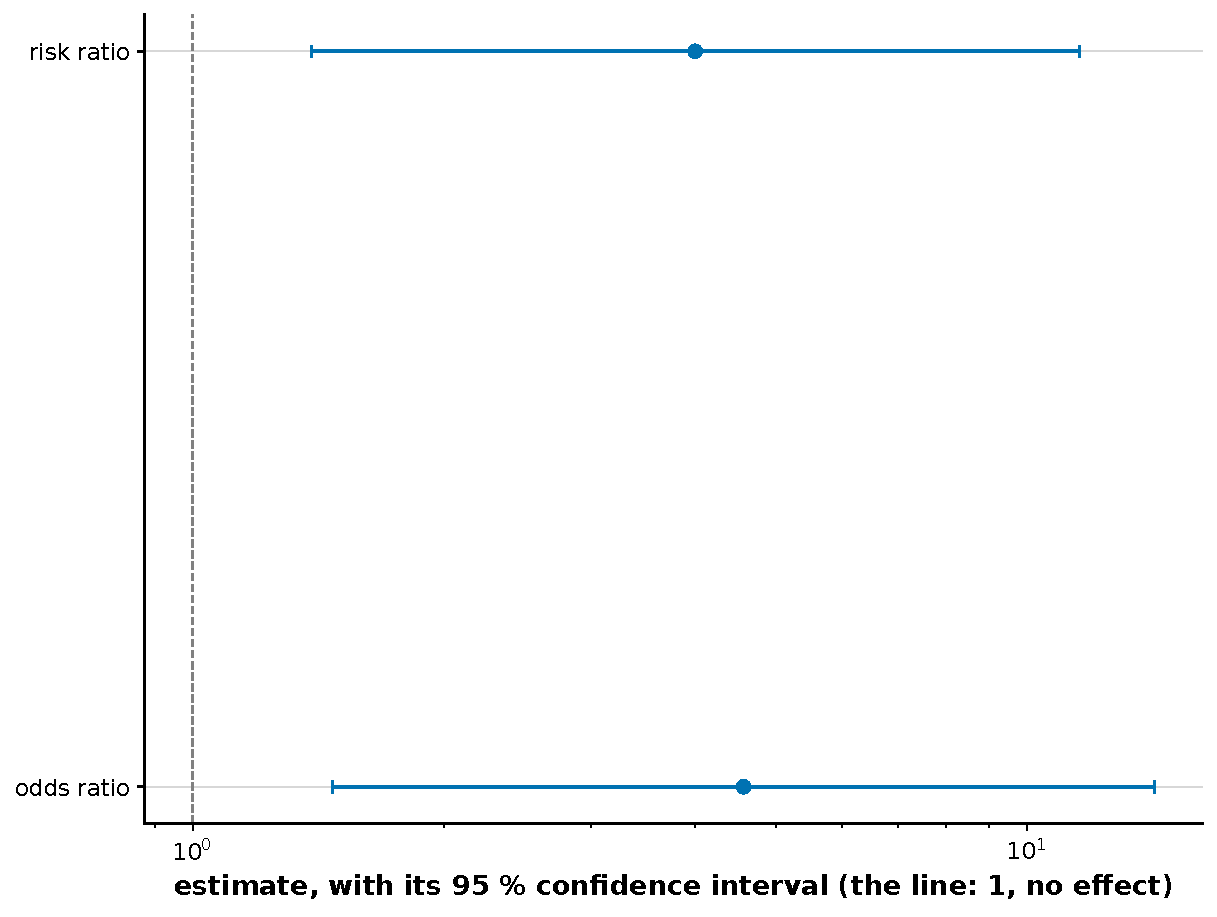
\includegraphics[width=0.72\textwidth,height=0.36\textheight,keepaspectratio]{figures/lesson22_example2_risk_ratios.pdf}
\captionof{figure}{Lesson 22, example 2: \code{risk\_\allowbreak{}ratios.\allowbreak{}png}.}
\end{minipage}\end{center}
\section*{Example 3}
How good is a quick test, against the truth from a slow lab test?
\begin{lstlisting}[style=py]
import simplydata as sdata
table = sdata.table(sdata.get_example("clinic"))
table.compare_to_truth("rapid_test", truth="infected")
table.compare_to_truth("rapid_test", truth="infected", prevalence=1)
\end{lstlisting}
\whateachline
\begin{lineexplain}
  \item[1] Load simplydata.
  \item[2] 50 of the 200 patients have the infection.
  \item[3] Of 1000 people like these, 250 have it: the test finds 195 (sensitivity 78 \%) and misses 55. Of the 750 without it, 50 test positive by mistake (specificity 93.3 \%).
  \item[4] Where only 1 \% have it, the same test gives 74 positives in 1000 people, and only 8 of them really have it: most positives are false alarms.
\end{lineexplain}
\printedoutput{output/lesson22_example3.txt}
\section*{Example 4}
Do a nurse and a doctor agree on how ill each patient looks?
\begin{lstlisting}[style=py]
import simplydata as sdata
table = sdata.table(sdata.get_example("clinic"))
table.agreement_between("nurse_rating", "doctor_rating")
\end{lstlisting}
\whateachline
\begin{lineexplain}
  \item[1] Load simplydata.
  \item[2] The clinic table.
  \item[3] They agree on 136 of 200 patients (68 \%); by chance alone they would agree on about 34 \%. Cohen's kappa = 0.516: they agree about half of the way from chance to perfect.
\end{lineexplain}
\printedoutput{output/lesson22_example4.txt}
\section*{Example 5}
More, optional (needs R): a score such as CRP has no single cut-off; each cut-off trades found cases against false alarms.
\begin{lstlisting}[style=py]
import simplydata as sdata
table = sdata.table(sdata.get_example("clinic"))
table.compare_to_truth("crp", truth="infected")
table.compare_accuracy("crp", "procalcitonin", truth="infected")
chart = table.start_chart()
chart.trade_off_curve(score=["crp", "procalcitonin"], truth="infected")
chart.save("trade_off.png")
\end{lstlisting}
\whateachline
\begin{lineexplain}
  \item[1] Load simplydata.
  \item[2] The clinic table.
  \item[3] AUC 0.893: a person who has it scores higher than one who does not in 89 of 100 such pairs. The best cut-off by Youden's index is 2.15.
  \item[4] AUC 0.893 against 0.715, a difference of 0.177 (0.085 to 0.270), on the same patients: CRP tells better who has it (DeLong's test, p = 0.0002).
  \item[5] Start a chart.
  \item[6] Both trade-off (ROC) curves: CRP climbs faster to the top left than procalcitonin.
  \item[7] Save it.
\end{lineexplain}
\printedoutput{output/lesson22_example5.txt}
\begin{center}\begin{minipage}{\linewidth}\centering
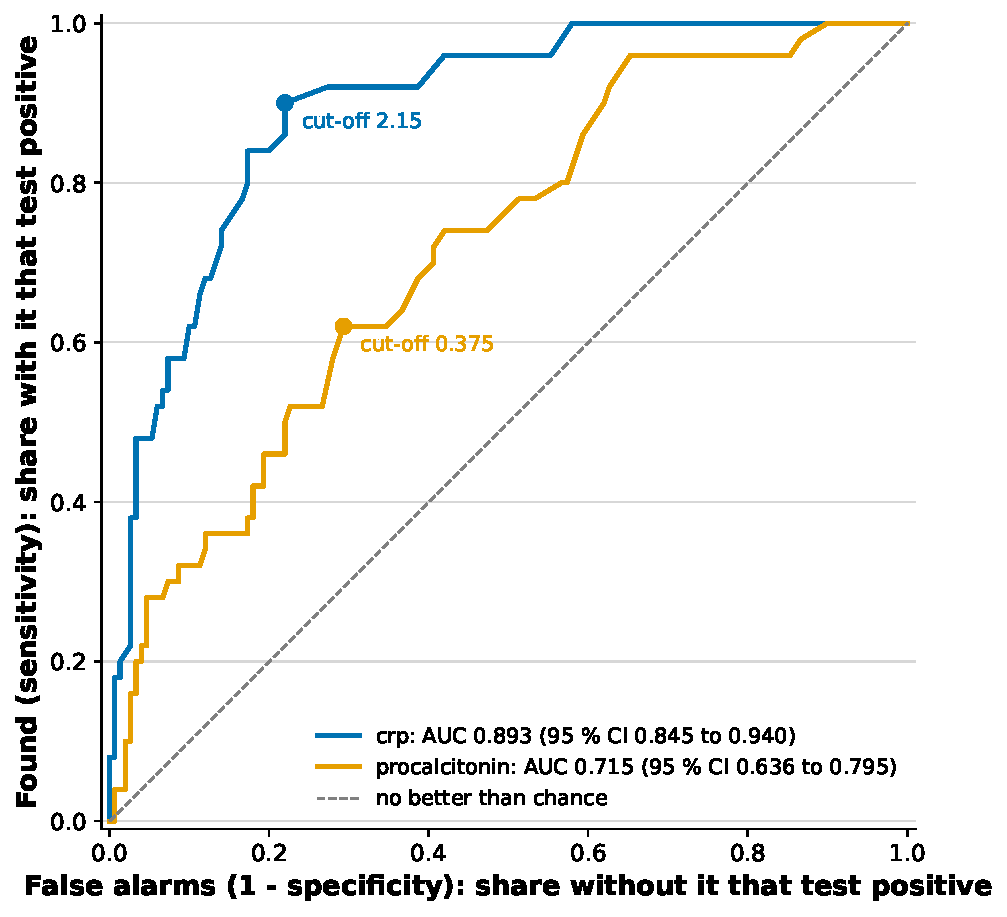
\includegraphics[width=0.72\textwidth,height=0.36\textheight,keepaspectratio]{figures/lesson22_example5_trade_off.pdf}
\captionof{figure}{Lesson 22, example 5: \code{trade\_\allowbreak{}off.\allowbreak{}png}.}
\end{minipage}\end{center}
\section*{Example 6}
More, optional (needs R): do two blood-pressure devices agree?
\begin{lstlisting}[style=py]
import simplydata as sdata
table = sdata.table(sdata.get_example("clinic"))
table.limits_of_agreement("device_a", "device_b")
chart = table.start_chart()
chart.difference_dots(first="device_a", second="device_b")
chart.save("devices.png")
\end{lstlisting}
\whateachline
\begin{lineexplain}
  \item[1] Load simplydata.
  \item[2] The clinic table.
  \item[3] Device A reads on average 2.18 lower, and 95 \% of the differences lie between -11.7 and 7.33.
  \item[4] Start a chart.
  \item[5] The Bland-Altman chart: each difference (first minus second) against the average of the two, with the limits of agreement.
  \item[6] Save it.
\end{lineexplain}
\printedoutput{output/lesson22_example6.txt}
\begin{center}\begin{minipage}{\linewidth}\centering
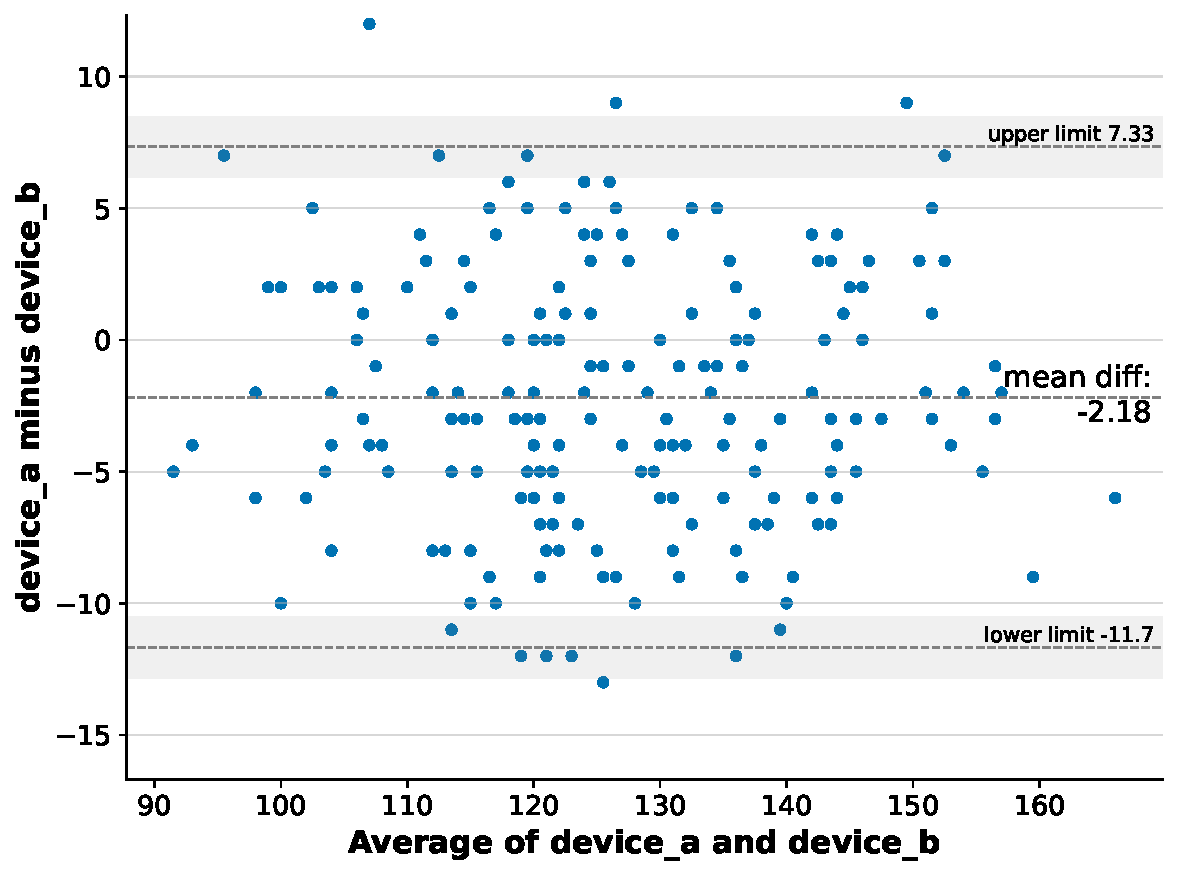
\includegraphics[width=0.72\textwidth,height=0.36\textheight,keepaspectratio]{figures/lesson22_example6_devices.pdf}
\captionof{figure}{Lesson 22, example 6: \code{devices.\allowbreak{}png}.}
\end{minipage}\end{center}
\section*{Example 7}
More, optional (needs R): do five questions on satisfaction with care (\code{item\_\allowbreak{}1} to \code{item\_\allowbreak{}5}) hang together?
\begin{lstlisting}[style=py]
import simplydata as sdata
table = sdata.table(sdata.get_example("clinic"))
table.reliability_of(["item_1", "item_2", "item_3", "item_4", "item_5"])
\end{lstlisting}
\whateachline
\begin{lineexplain}
  \item[1] Load simplydata.
  \item[2] The clinic table.
  \item[3] Cronbach's alpha = 0.865 (0.833 to 0.893); leaving out any one item lowers it.
\end{lineexplain}
\printedoutput{output/lesson22_example7.txt}
\section*{Example 8}
More, optional: risks allowing for a third column, and rates per patient-day.
\begin{lstlisting}[style=py]
import simplydata as sdata
table = sdata.table(sdata.get_example("clinic"))
table.compare_risks("infected", for_each_group_in="ward", allowing_for="age_group")
table.rate_of("infections", time="patient_days", for_each_group_in="ward")
\end{lstlisting}
\whateachline
\begin{lineexplain}
  \item[1] Load simplydata.
  \item[2] The clinic table.
  \item[3] Mantel-Haenszel odds ratio 1.76 (0.911 to 3.40), about the same as 1.71 without allowing for age (the interval of its risk ratio needs R epiR).
  \item[4] 2.22 infections per 1000 patient-days in ward A and 10.0 in ward B, each with its exact interval; \code{compare\_\allowbreak{}rates} compares them.
\end{lineexplain}
\printedoutput{output/lesson22_example8.txt}
\begin{goodtoknow}
\begin{itemize}
  \item This lesson is optional, for the life sciences (medicine, biology, ecology); no other lesson needs it. Examples 1 to 4 are the core; examples 5 to 8 are more, for when you need them.
  \item Give absolute risks first. A risk ratio of 0.5 can mean 2 in 100 instead of 4, or 20 instead of 40: the same ratio, a very different number of people helped.
  \item When the interval of the difference includes 0, the number needed for one event fewer (or more) has an interval that runs through infinity: the data fit fewer events, no change and more. Task 1 shows one.
  \item Odds are not risks. When the outcome is common (over 10 \%), the odds ratio lies further from 1 than the risk ratio, so say which one you report.
  \item Sensitivity and specificity belong to the test; the share of positives that are real also depends on how common the condition is. Counts of 1000 people make this easy to see.
  \item Agreement is not correlation: two raters (or devices) can rise and fall together and still differ every time.
\end{itemize}
\end{goodtoknow}
\begin{tryit}
\begin{enumerate}
  \item Compare the risk of \code{\textquotedbl{}infected\textquotedbl{}} between the wards, against \code{\textquotedbl{}ward A\textquotedbl{}}. Does the interval of the difference leave out 0?
  \item How good is the rapid test where only 2 \% have the infection? Of the positive results, how many really have it?
  \item Complete the started lines to draw the two ratios of task 1: risks = \code{table.\allowbreak{}compare\_\allowbreak{}risks(\textquotedbl{}infected\textquotedbl{},\allowbreak{} for\_\allowbreak{}each\_\allowbreak{}group\_\allowbreak{}in=\textquotedbl{}ward\textquotedbl{},\allowbreak{} against=\textquotedbl{}ward A\textquotedbl{})}, then \code{risks.\allowbreak{}keep\_\allowbreak{}rows\_\allowbreak{}where(\textquotedbl{}measure\textquotedbl{},\allowbreak{} is\_\allowbreak{}one\_\allowbreak{}of=[.\allowbreak{}.\allowbreak{}.\allowbreak{}])}, then chart = \code{risks.\allowbreak{}start\_\allowbreak{}chart()} and \code{chart.\allowbreak{}forest\_\allowbreak{}plot(.\allowbreak{}.\allowbreak{}.\allowbreak{})}.
\end{enumerate}
Worked solutions: page~\pageref{solutions:22}, or type \code{sdata.\allowbreak{}show\_\allowbreak{}lesson(22,\allowbreak{} solutions=True)}.
\end{tryit}
\par\noindent{\small\sffamily\textbf{Words in this lesson:} \hyperref[word:table.compare-risks]{\code{table.\allowbreak{}compare\_\allowbreak{}risks()}}, \hyperref[word:forest-plot]{\code{chart.\allowbreak{}forest\_\allowbreak{}plot()}}, \hyperref[word:table.compare-to-truth]{\code{table.\allowbreak{}compare\_\allowbreak{}to\_\allowbreak{}truth()}}, \hyperref[word:table.agreement-between]{\code{table.\allowbreak{}agreement\_\allowbreak{}between()}}, \hyperref[word:trade-off-curve]{\code{chart.\allowbreak{}trade\_\allowbreak{}off\_\allowbreak{}curve()}}, \hyperref[word:table.compare-accuracy]{\code{table.\allowbreak{}compare\_\allowbreak{}accuracy()}}, \hyperref[word:table.limits-of-agreement]{\code{table.\allowbreak{}limits\_\allowbreak{}of\_\allowbreak{}agreement()}}, \hyperref[word:difference-dots]{\code{chart.\allowbreak{}difference\_\allowbreak{}dots()}}, \hyperref[word:table.reliability-of]{\code{table.\allowbreak{}reliability\_\allowbreak{}of()}}, \hyperref[word:table.rate-of]{\code{table.\allowbreak{}rate\_\allowbreak{}of()}}.\par}

\chapter{Time series: dates, missing days, time windows and trend}\label{lesson:23}
\begin{learnbox}
\begin{itemize}
  \item how to make a run of dates, and add the days that are missing from a daily table
  \item how to average over a window of time, such as the last 7 days
  \item how to smooth a noisy series, and test whether it has a trend
\end{itemize}
\end{learnbox}
\begin{needsr}\code{find\_\allowbreak{}trend\_\allowbreak{}of()} and its test run R's own code, the same code R users run. Install it once: pip install \code{\textquotedbl{}simplydata[r]\textquotedbl{}}, then R from https://cran.r-project.org, then in R: \code{install.\allowbreak{}packages(c(\textquotedbl{}trend\textquotedbl{}))}. Without R these words print a message that says what to install.\end{needsr}
\section*{Example 1}
Time series are readings in time order: one a day, a month or a second. A run of dates is the backbone of such a table.
\begin{lstlisting}[style=py]
import simplydata as sdata
days = sdata.make_run_of_dates("2026-01-01", to="2026-12-31", every="month")
days.show()
\end{lstlisting}
\whateachline
\begin{lineexplain}
  \item[1] Load simplydata.
  \item[2] 12 dates, the first of each month of 2026, in a table with one column, date.
  \item[3] Show them.
\end{lineexplain}
\printedoutput{output/lesson23_example1.txt}
\section*{Example 2}
Two river stations measured the water level and nitrate every day for two years, but some days are missing: their rows are simply not there. Words that need even steps stop with a message, so add the missing days first and fill them in.
\begin{lstlisting}[style=py]
import simplydata as sdata
table = sdata.table(sdata.get_example("river"))
table.add_missing_dates("date", every="day", for_each_group_in="station")
table.fill_empty_cells_in("nitrate", with_the="line between neighbours", sorted_by="date", for_each_group_in="station")
table.fill_empty_cells_in("level", with_the="line between neighbours", sorted_by="date", for_each_group_in="station")
\end{lstlisting}
\whateachline
\begin{lineexplain}
  \item[1] Load simplydata.
  \item[2] Daily date, station, level and nitrate.
  \item[3] 15 days were missing (6 at Station A, 9 at Station B); their rows are added with empty cells.
  \item[4] The 15 empty nitrate cells get the value on the straight line between their neighbours.
  \item[5] The same for the level: 23 cells (a few were empty already).
\end{lineexplain}
\printedoutput{output/lesson23_example2.txt}
\section*{Example 3}
Daily readings are noisy. A time window averages the readings of the last 7 days; a smoother averages the readings on both sides of each day.
\begin{lstlisting}[style=py]
import simplydata as sdata
table = sdata.table(sdata.get_example("river"))
table.add_missing_dates("date", every="day", for_each_group_in="station")
table.fill_empty_cells_in("nitrate", with_the="line between neighbours", sorted_by="date", for_each_group_in="station")
table.add_rolling_column("week_average", from_column="nitrate", window="7 days", sorted_by="date", for_each_group_in="station")
table.add_smoothed_column("nitrate_smoothed", from_column="nitrate", method="moving average", window=31, sorted_by="date", for_each_group_in="station")
chart = table.start_chart()
chart.draw_lines(x="date", y="nitrate_smoothed", colour="station")
chart.save("nitrate.png")
\end{lstlisting}
\whateachline
\begin{lineexplain}
  \item[1] Load simplydata.
  \item[2] The river table.
  \item[3] Add the missing days.
  \item[4] Fill them in.
  \item[5] Each \code{week\_\allowbreak{}average} is the average nitrate of the 7 days up to that day, for each station.
  \item[6] A moving average over 31 days centred on each day; the first and last 15 days have no full window, so they are empty (as R stats::\code{filter(x,\allowbreak{} rep(1 / 31,\allowbreak{} 31),\allowbreak{} sides = 2)}).
  \item[7] Start a chart.
  \item[8] The smoothed nitrate, one line per station: Station A creeps up, Station B goes down.
  \item[9] Save it.
\end{lineexplain}
\printedoutput{output/lesson23_example3.txt}
\begin{center}\begin{minipage}{\linewidth}\centering
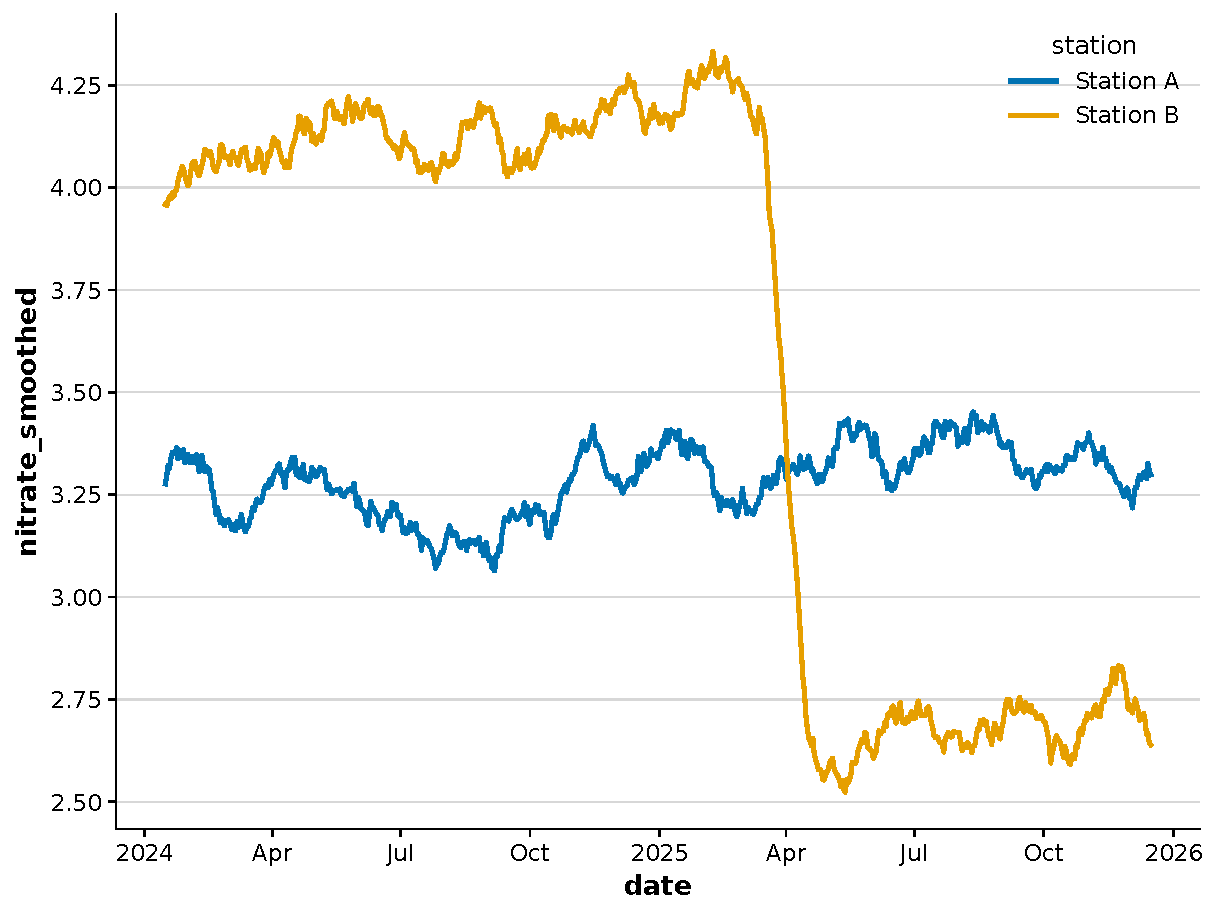
\includegraphics[width=0.72\textwidth,height=0.36\textheight,keepaspectratio]{figures/lesson23_example3_nitrate.pdf}
\captionof{figure}{Lesson 23, example 3: \code{nitrate.\allowbreak{}png}.}
\end{minipage}\end{center}
\section*{Example 4}
Is there a steady trend? \code{find\_\allowbreak{}trend\_\allowbreak{}of} gives the slope (Sen's slope, the middle of the slopes between all pairs of days) and the Mann-Kendall test.
\begin{lstlisting}[style=py]
import simplydata as sdata
table = sdata.table(sdata.get_example("river"))
table.find_trend_of("nitrate", sorted_by="date", for_each_group_in="station")
\end{lstlisting}
\whateachline
\begin{lineexplain}
  \item[1] Load simplydata.
  \item[2] The river table.
  \item[3] Station A rises by 0.0708 a year (p = 0.003); Station B falls by 0.927 a year (p \textless{} 0.0001). R's trend::\code{sens.\allowbreak{}slope()} and trend::\code{mk.\allowbreak{}test()} give the same numbers.
\end{lineexplain}
\printedoutput{output/lesson23_example4.txt}
\begin{goodtoknow}
\begin{itemize}
  \item \code{sorted\_\allowbreak{}by=} is the time column: it gives the order and the time between readings. \code{for\_\allowbreak{}each\_\allowbreak{}group\_\allowbreak{}in=} gives one series per group, here one per station.
  \item \code{window=7} is 7 rows; \code{window=\textquotedbl{}7 days\textquotedbl{}} is 7 days of time, whatever the number of rows.
  \item \code{find\_\allowbreak{}trend\_\allowbreak{}of} needs no even steps and no filling: empty cells are left out.
\end{itemize}
\end{goodtoknow}
\begin{tryit}
\begin{enumerate}
  \item Make a run of dates for every day of March 2026.
  \item Add a column with the average level of the last 30 days at each station.
  \item Smooth the level of each station with a moving average over 61 days instead of 31, and draw it. What does the wider window do?
\end{enumerate}
Worked solutions: page~\pageref{solutions:23}, or type \code{sdata.\allowbreak{}show\_\allowbreak{}lesson(23,\allowbreak{} solutions=True)}.
\end{tryit}
\par\noindent{\small\sffamily\textbf{Words in this lesson:} \hyperref[word:sdata.make-run-of-dates]{\code{sdata.\allowbreak{}make\_\allowbreak{}run\_\allowbreak{}of\_\allowbreak{}dates()}}, \hyperref[word:table.add-missing-dates]{\code{table.\allowbreak{}add\_\allowbreak{}missing\_\allowbreak{}dates()}}, \hyperref[word:table.fill-empty-cells-in]{\code{table.\allowbreak{}fill\_\allowbreak{}empty\_\allowbreak{}cells\_\allowbreak{}in()}}, \hyperref[word:table.add-rolling-column]{\code{table.\allowbreak{}add\_\allowbreak{}rolling\_\allowbreak{}column()}}, \hyperref[word:table.add-smoothed-column]{\code{table.\allowbreak{}add\_\allowbreak{}smoothed\_\allowbreak{}column()}}, \hyperref[word:table.find-trend-of]{\code{table.\allowbreak{}find\_\allowbreak{}trend\_\allowbreak{}of()}}, \hyperref[word:draw-lines]{\code{chart.\allowbreak{}draw\_\allowbreak{}lines()}}.\par}

\chapter{Forecasts: the next months, checked first}\label{lesson:24}
\begin{learnbox}
\begin{itemize}
  \item how to draw a series over time, and each year on top of the others (a seasonal chart)
  \item how to forecast the next months, starting from the simplest forecast
  \item how to check a forecast on months it has not seen before trusting it
\end{itemize}
\end{learnbox}
\begin{needsr}\code{forecast()} and \code{compare\_\allowbreak{}forecasts\_\allowbreak{}for()} run R's own code, the same code R users run. Install it once: pip install \code{\textquotedbl{}simplydata[r]\textquotedbl{}}, then R from https://cran.r-project.org, then in R: \code{install.\allowbreak{}packages(c(\textquotedbl{}forecast\textquotedbl{}))}. Without R these words print a message that says what to install.\end{needsr}
\section*{Example 1}
Two museums counted their visitors every month for twelve years. A chart over time comes first: it shows the trend and the season at a glance.
\begin{lstlisting}[style=py]
import simplydata as sdata
table = sdata.table(sdata.get_example("visitors"))
chart = table.start_chart()
chart.draw_lines(x="month", y="visitors", colour="museum")
chart.save("visitor_lines.png")
\end{lstlisting}
\whateachline
\begin{lineexplain}
  \item[1] Load simplydata.
  \item[2] Monthly visitors to two made-up museums, 2014 to 2025: month, museum, visitors.
  \item[3] Start a chart of the table.
  \item[4] One line per museum: both rise year after year, with a peak every summer.
  \item[5] Save it.
\end{lineexplain}
\printedoutput{output/lesson24_example1.txt}
\begin{center}\begin{minipage}{\linewidth}\centering
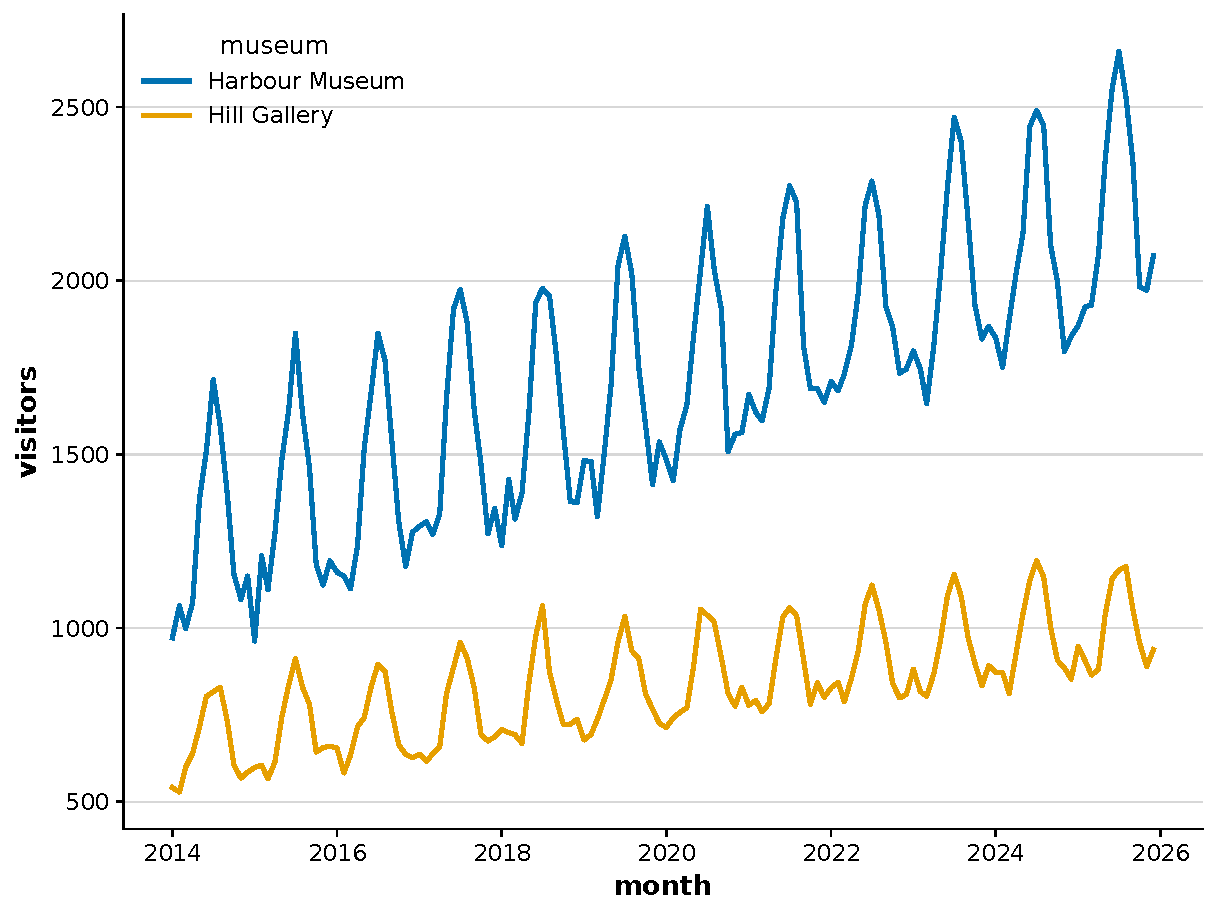
\includegraphics[width=0.72\textwidth,height=0.36\textheight,keepaspectratio]{figures/lesson24_example1_visitor_lines.pdf}
\captionof{figure}{Lesson 24, example 1: \code{visitor\_\allowbreak{}lines.\allowbreak{}png}.}
\end{minipage}\end{center}
\section*{Example 2}
A seasonal chart puts each year on top of the others, January to December. It needs no new word: take the month and the year out of the date, then draw one line per year.
\begin{lstlisting}[style=py]
import simplydata as sdata
table = sdata.table(sdata.get_example("visitors"))
table.keep_rows_where("museum", is_equal_to="Harbour Museum")
table.add_column_with_part_of_date("month_name", from_column="month", part="month")
table.add_column_with_part_of_date("year", from_column="month", part="year")
chart = table.start_chart()
chart.draw_lines(x="month_name", y="visitors", colour="year")
chart.save("visitor_seasons.png")
\end{lstlisting}
\whateachline
\begin{lineexplain}
  \item[1] Load simplydata.
  \item[2] The visitors table.
  \item[3] Keep one museum: 144 of 288 rows.
  \item[4] The month of each date.
  \item[5] The year of each date.
  \item[6] Start a chart.
  \item[7] Twelve lines, one per year, all with the same summer peak; later years lie higher.
  \item[8] Save it.
\end{lineexplain}
\printedoutput{output/lesson24_example2.txt}
\begin{center}\begin{minipage}{\linewidth}\centering
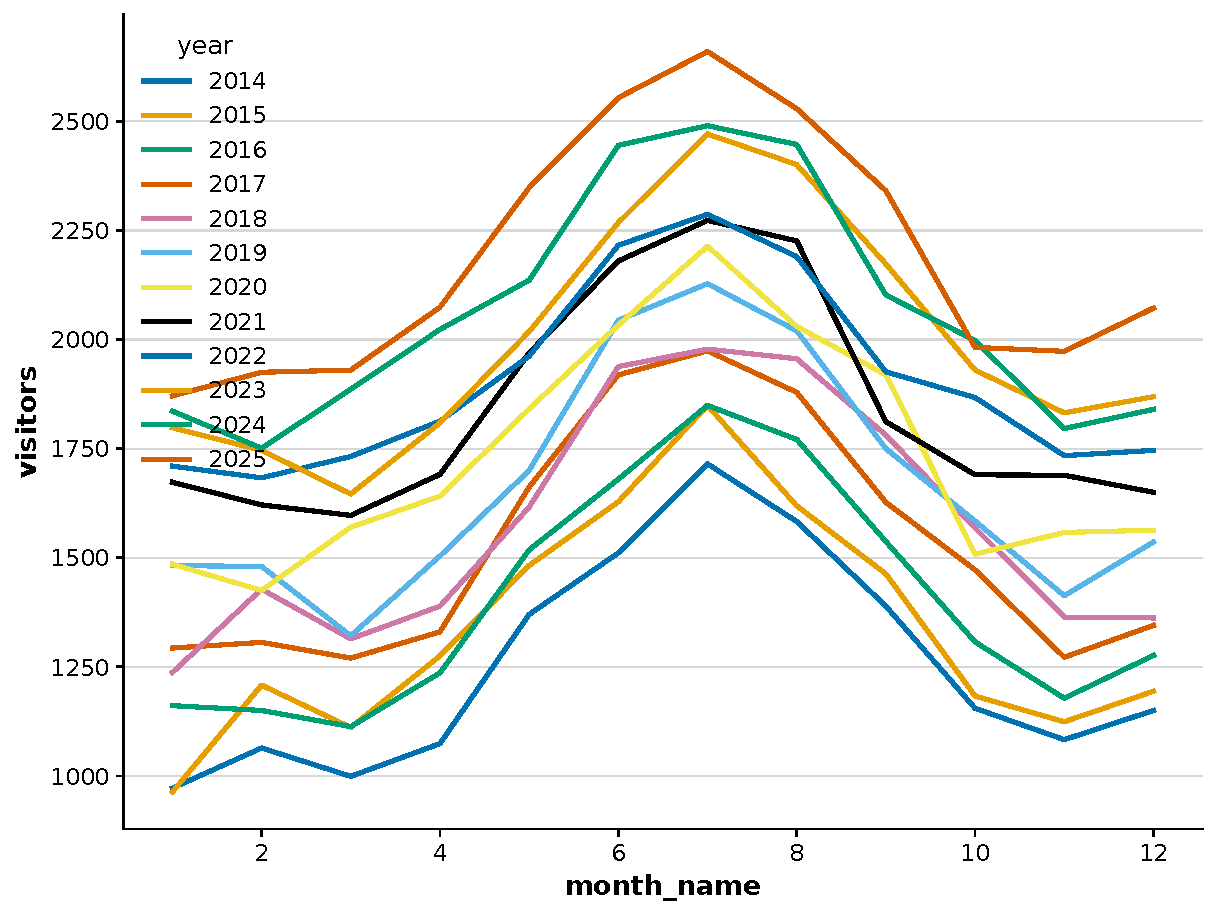
\includegraphics[width=0.72\textwidth,height=0.36\textheight,keepaspectratio]{figures/lesson24_example2_visitor_seasons.pdf}
\captionof{figure}{Lesson 24, example 2: \code{visitor\_\allowbreak{}seasons.\allowbreak{}png}.}
\end{minipage}\end{center}
\section*{Example 3}
Start with the simplest forecast: every future month is the last value. Any better method must beat it.
\begin{lstlisting}[style=py]
import simplydata as sdata
table = sdata.table(sdata.get_example("visitors"))
table.forecast("visitors", sorted_by="month", steps_ahead=12, method="last value", for_each_group_in="museum")
\end{lstlisting}
\whateachline
\begin{lineexplain}
  \item[1] Load simplydata.
  \item[2] The visitors table.
  \item[3] Harbour Museum: 2072 every month (95 \% prediction interval 1746 to 2398 next month, 944 to 3200 in a year). The printout warns that the errors still hold a pattern: the season is missed.
\end{lineexplain}
\printedoutput{output/lesson24_example3.txt}
\section*{Example 4}
Exponential smoothing (Holt-Winters) follows the level, the trend and the season. Before trusting it, hold back the last year, forecast it from the years before, and see how far off it is.
\begin{lstlisting}[style=py]
import simplydata as sdata
table = sdata.table(sdata.get_example("visitors"))
table.forecast("visitors", sorted_by="month", steps_ahead=12, repeats_every="year", check_on_last=12, for_each_group_in="museum")
table.compare_forecasts_for("visitors", sorted_by="month", repeats_every="year", for_each_group_in="museum")
\end{lstlisting}
\whateachline
\begin{lineexplain}
  \item[1] Load simplydata.
  \item[2] The visitors table.
  \item[3] Fitted on all but the last 12 months, it was off by 64.7 visitors a month on average at the Harbour Museum (2.93 \%) and 21.5 at the Hill Gallery (2.20 \%).
  \item[4] Four methods on the same held-back year: exponential smoothing is best for both museums (MASE 0.469 and 0.348; below 1 is better than repeating last year's month).
\end{lineexplain}
\printedoutput{output/lesson24_example4.txt}
\section*{Example 5}
Now forecast the next year from all the data, and draw it after the lines.
\begin{lstlisting}[style=py]
import simplydata as sdata
table = sdata.table(sdata.get_example("visitors"))
table.forecast("visitors", sorted_by="month", steps_ahead=12, repeats_every="year", for_each_group_in="museum")
chart = table.start_chart()
chart.draw_lines(x="month", y="visitors", colour="museum")
chart.forecast(steps_ahead=12, repeats_every="year")
chart.save("visitor_forecast.png")
\end{lstlisting}
\whateachline
\begin{lineexplain}
  \item[1] Load simplydata.
  \item[2] The visitors table.
  \item[3] Harbour Museum next month: 2016 visitors (95 \% prediction interval 1887 to 2146); Hill Gallery: 947 (887 to 1008). R's \code{HoltWinters()} and \code{forecast()} give the same numbers.
  \item[4] Start a chart.
  \item[5] The data, one line per museum.
  \item[6] The forecast as a dashed line after the data, with its interval band.
  \item[7] Save it.
\end{lineexplain}
\printedoutput{output/lesson24_example5.txt}
\begin{center}\begin{minipage}{\linewidth}\centering
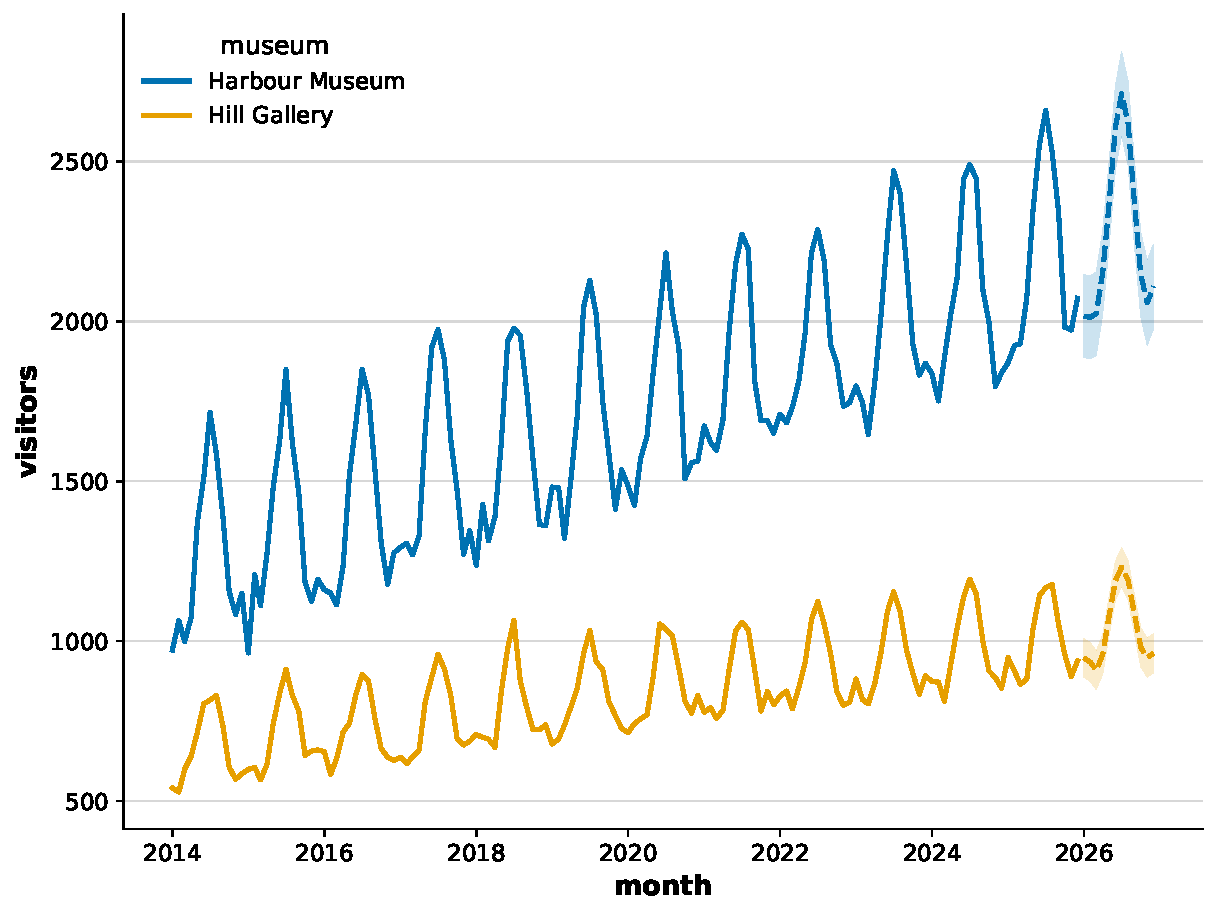
\includegraphics[width=0.72\textwidth,height=0.36\textheight,keepaspectratio]{figures/lesson24_example5_visitor_forecast.pdf}
\captionof{figure}{Lesson 24, example 5: \code{visitor\_\allowbreak{}forecast.\allowbreak{}png}.}
\end{minipage}\end{center}
\begin{goodtoknow}
\begin{itemize}
  \item \code{repeats\_\allowbreak{}every=\textquotedbl{}year\textquotedbl{}} turns into 12 rows for monthly data (7 for \code{\textquotedbl{}week\textquotedbl{}} with daily data).
  \item A prediction interval says where the next values will probably fall. It widens the further ahead you look.
  \item \code{check\_\allowbreak{}on\_\allowbreak{}last=12} holds back the last 12 readings: a forecast is only as good as its check on data it has not seen.
\end{itemize}
\end{goodtoknow}
\begin{tryit}
\begin{enumerate}
  \item Forecast the Harbour Museum with \code{method=\textquotedbl{}same season last time\textquotedbl{}}. How does it compare with exponential smoothing?
  \item Check the \code{\textquotedbl{}straight on\textquotedbl{}} method (the line from the first reading to the last) on the last 12 months of the Hill Gallery.
\end{enumerate}
Worked solutions: page~\pageref{solutions:24}, or type \code{sdata.\allowbreak{}show\_\allowbreak{}lesson(24,\allowbreak{} solutions=True)}.
\end{tryit}
\par\noindent{\small\sffamily\textbf{Words in this lesson:} \hyperref[word:draw-lines]{\code{chart.\allowbreak{}draw\_\allowbreak{}lines()}}, \hyperref[word:table.add-column-with-part-of-date]{\code{table.\allowbreak{}add\_\allowbreak{}column\_\allowbreak{}with\_\allowbreak{}part\_\allowbreak{}of\_\allowbreak{}date()}}, \hyperref[word:table.forecast]{\code{table.\allowbreak{}forecast()}}, \hyperref[word:table.compare-forecasts-for]{\code{table.\allowbreak{}compare\_\allowbreak{}forecasts\_\allowbreak{}for()}}, \hyperref[word:forecast]{\code{chart.\allowbreak{}forecast()}}.\par}

\chapter{Cycles: spectra, filters, peaks, and steady or not}\label{lesson:25}
\begin{learnbox}
\begin{itemize}
  \item how to find the repeating cycles in a recording, and how strong each is (the spectrum)
  \item how to take out a hum, or keep only the slow cycles (filters)
  \item how to find the peaks and the dips of a signal
  \item more, if you want it: a smoother spectrum (Welch), and whether a series stays steady
\end{itemize}
\end{learnbox}
\begin{needsr}Only the last part, \code{check\_\allowbreak{}steady\_\allowbreak{}over\_\allowbreak{}time()} and its two tests, run R's own code, the same code R users run. Install it once: pip install \code{\textquotedbl{}simplydata[r]\textquotedbl{}}, then R from https://cran.r-project.org, then in R: \code{install.\allowbreak{}packages(c(\textquotedbl{}tseries\textquotedbl{}))}. Without R these words print a message that says what to install.\end{needsr}
\section*{Example 1}
A sensor gives 200 readings a second for 5 seconds. Which cycles does its signal hold? The spectrum splits a recording into its frequencies, like a prism splits light into colours.
\begin{lstlisting}[style=py]
import simplydata as sdata
table = sdata.table(sdata.get_example("sensor"))
table.find_spectrum_of("signal", sorted_by="time")
chart = table.start_chart()
chart.spectrum("signal", sorted_by="time")
chart.save("spectrum.png")
\end{lstlisting}
\whateachline
\begin{lineexplain}
  \item[1] Load simplydata.
  \item[2] Five seconds of a made-up sensor: time in seconds, signal and vibration.
  \item[3] The strongest cycle has frequency 5 per second (it repeats every 0.2 seconds) and holds 68 \% of the variance; next come 20 per second (11 \%) and a 50-per-second hum (4 \%).
  \item[4] Start a chart.
  \item[5] The same numbers as a chart: power against frequency on a log scale, the three strongest cycles labelled with how often they repeat.
  \item[6] Save it.
\end{lineexplain}
\printedoutput{output/lesson25_example1.txt}
\begin{center}\begin{minipage}{\linewidth}\centering
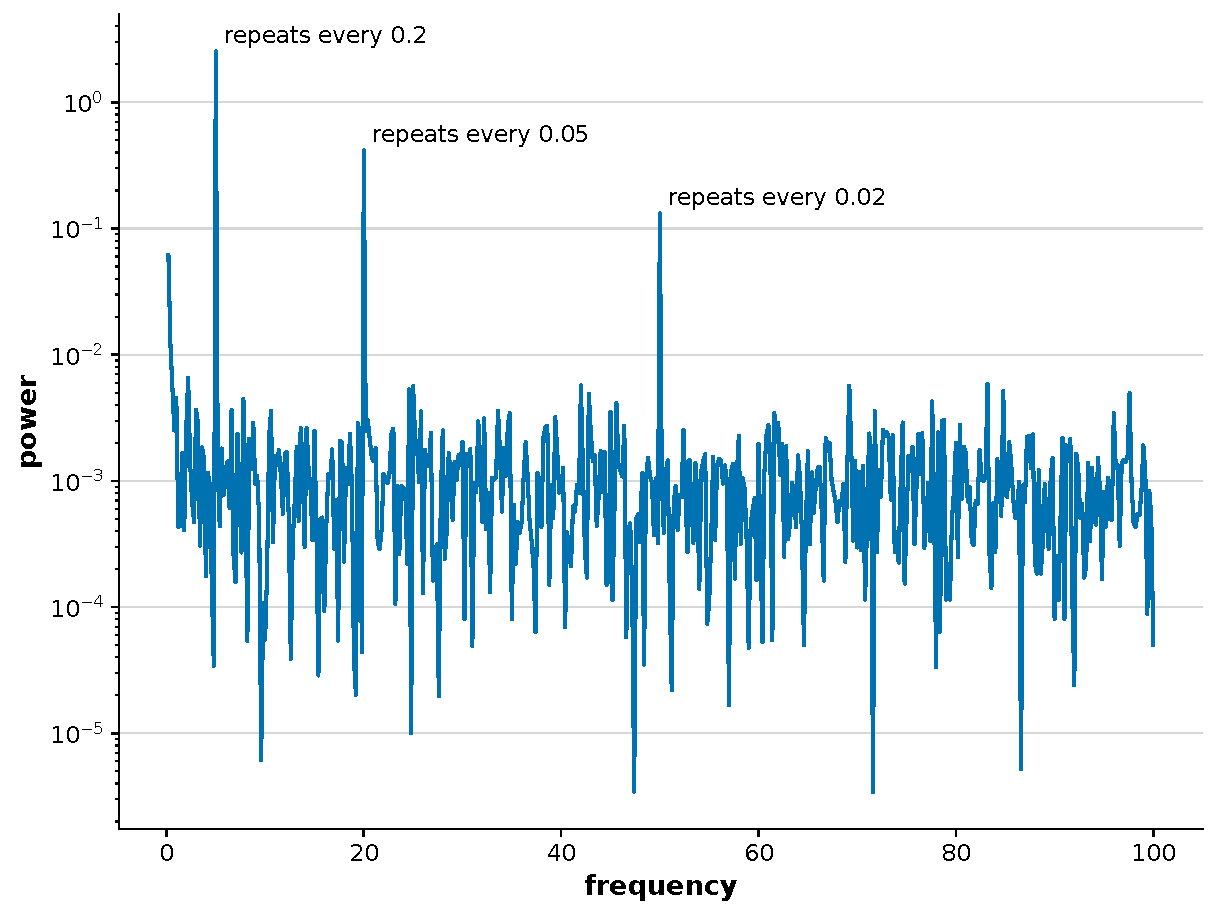
\includegraphics[width=0.72\textwidth,height=0.36\textheight,keepaspectratio]{figures/lesson25_example1_spectrum.pdf}
\captionof{figure}{Lesson 25, example 1: \code{spectrum.\allowbreak{}png}.}
\end{minipage}\end{center}
\section*{Example 2}
A filter keeps some frequencies and removes others. \code{remove\_\allowbreak{}at=50} takes out the hum; \code{keep\_\allowbreak{}below=10} keeps only the slow cycles.
\begin{lstlisting}[style=py]
import simplydata as sdata
table = sdata.table(sdata.get_example("sensor"))
table.add_filtered_column("no_hum", from_column="signal", remove_at=50, sorted_by="time")
table.find_spectrum_of("no_hum", sorted_by="time")
table.add_filtered_column("slow", from_column="signal", keep_below=10, sorted_by="time")
chart = table.start_chart()
chart.draw_lines(x="time", y="signal")
chart.draw_lines(x="time", y="slow")
chart.set_range_x(0, 1)
chart.save("filter.png")
\end{lstlisting}
\whateachline
\begin{lineexplain}
  \item[1] Load simplydata.
  \item[2] The sensor table.
  \item[3] A notch filter at 50 per second, run forwards and backwards so nothing moves in time.
  \item[4] The hum is gone: now 5 per second holds 71 \% and 20 per second 12 \% of the variance.
  \item[5] A Butterworth low-pass filter (steepness 4), as R signal::\code{filtfilt(signal::butter(4,\allowbreak{} 0.\allowbreak{}1),\allowbreak{} x)}.
  \item[6] Start a chart.
  \item[7] The raw signal.
  \item[8] The slow part only: a clean 5-per-second wave.
  \item[9] Show the first second.
  \item[10] Save it.
\end{lineexplain}
\printedoutput{output/lesson25_example2.txt}
\begin{center}\begin{minipage}{\linewidth}\centering
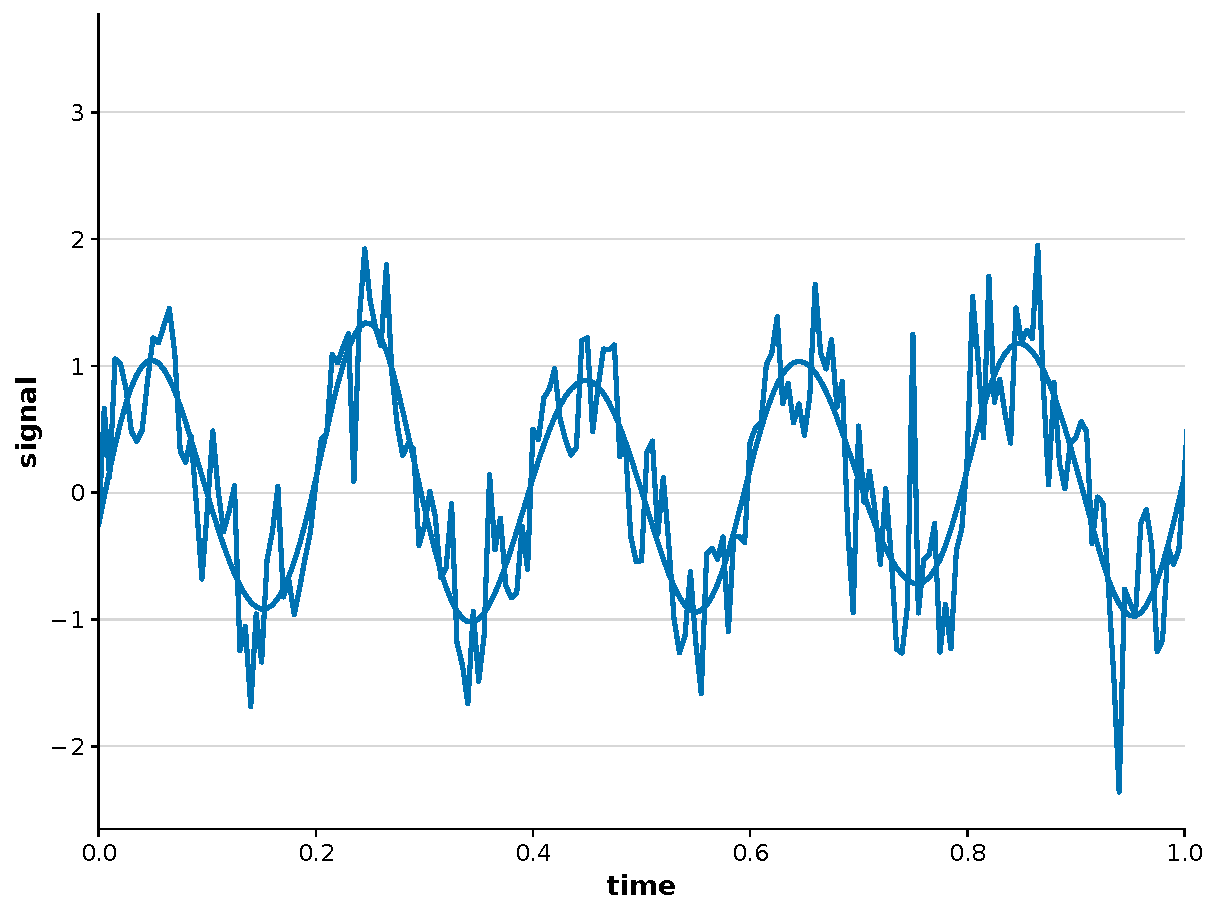
\includegraphics[width=0.72\textwidth,height=0.36\textheight,keepaspectratio]{figures/lesson25_example2_filter.pdf}
\captionof{figure}{Lesson 25, example 2: \code{filter.\allowbreak{}png}.}
\end{minipage}\end{center}
\section*{Example 3}
Peaks are readings higher than both neighbours; dips are readings lower than both. Conditions keep only the ones that matter.
\begin{lstlisting}[style=py]
import simplydata as sdata
table = sdata.table(sdata.get_example("sensor"))
table.find_each_peak_that("signal", sorted_by="time", is_at_least=2.5)
table.find_each_dip_that("signal", sorted_by="time", is_at_most=-2)
chart = table.start_chart()
chart.draw_lines(x="time", y="signal")
chart.peak_dots(is_at_least=2.5)
chart.save("peaks.png")
\end{lstlisting}
\whateachline
\begin{lineexplain}
  \item[1] Load simplydata.
  \item[2] The sensor table.
  \item[3] One peak is at least 2.5 high: 3.48 at time 3.885, a spike. R's pracma::\code{findpeaks()} finds the same.
  \item[4] \code{find\_\allowbreak{}each\_\allowbreak{}dip\_\allowbreak{}that} is \code{find\_\allowbreak{}each\_\allowbreak{}peak\_\allowbreak{}that} upside down: one dip goes down to -2 or lower, -2.36 at time 0.94.
  \item[5] Start a chart.
  \item[6] The signal.
  \item[7] A mark on the peak.
  \item[8] Save it.
\end{lineexplain}
\printedoutput{output/lesson25_example3.txt}
\begin{center}\begin{minipage}{\linewidth}\centering
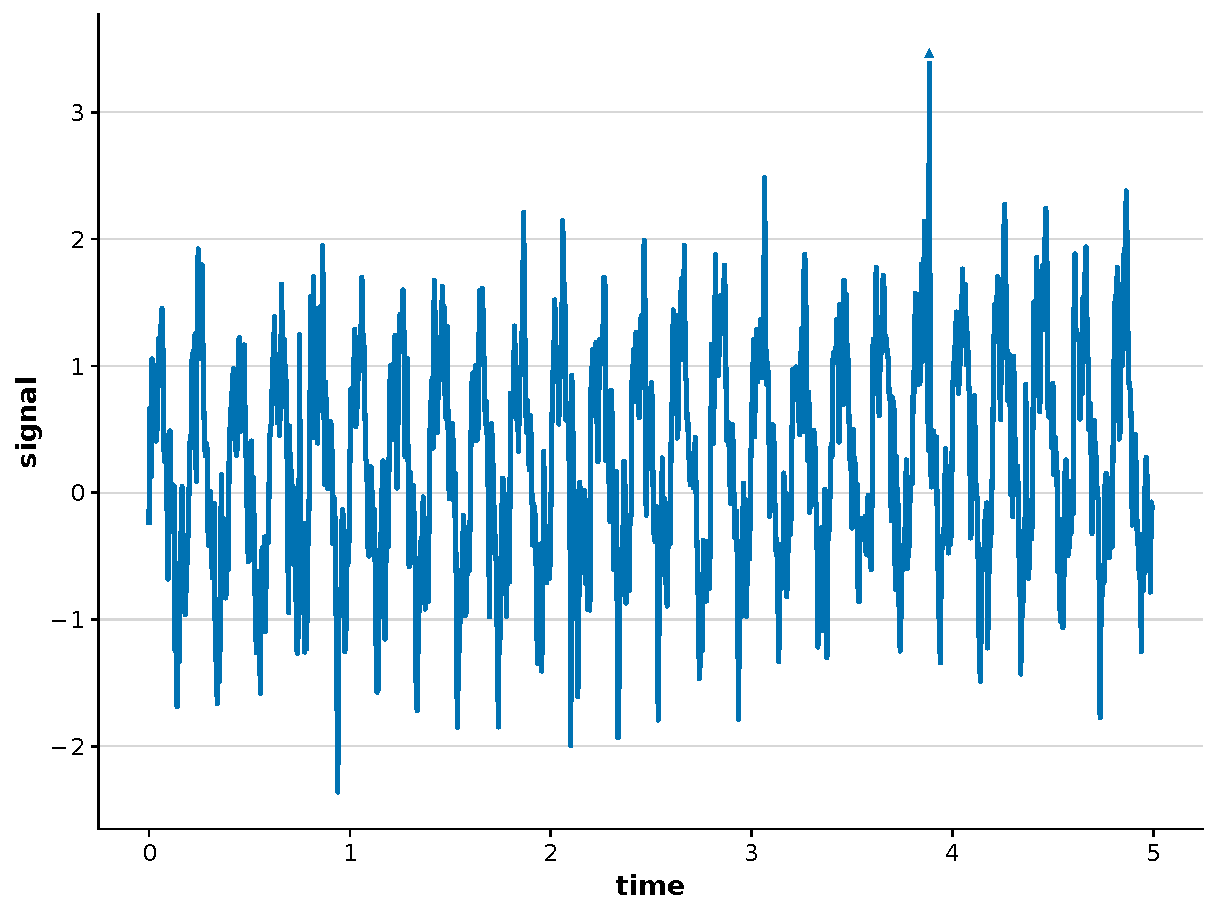
\includegraphics[width=0.72\textwidth,height=0.36\textheight,keepaspectratio]{figures/lesson25_example3_peaks.pdf}
\captionof{figure}{Lesson 25, example 3: \code{peaks.\allowbreak{}png}.}
\end{minipage}\end{center}
\section*{Example 4}
More (if you want it): Welch's method averages the spectra of overlapping pieces of the recording. The spectrum is smoother but coarser.
\begin{lstlisting}[style=py]
import simplydata as sdata
table = sdata.table(sdata.get_example("sensor"))
table.find_spectrum_of("signal", sorted_by="time", method="welch", window=200)
\end{lstlisting}
\whateachline
\begin{lineexplain}
  \item[1] Load simplydata.
  \item[2] The sensor table.
  \item[3] Pieces of 200 readings with half overlap: the same three cycles stand out (5, 20 and 50 per second).
\end{lineexplain}
\printedoutput{output/lesson25_example4.txt}
\section*{Example 5}
More (if you want it; needs R): some forecasts (ARIMA) assume the series is steady: the same average and spread all the way through. \code{check\_\allowbreak{}steady\_\allowbreak{}over\_\allowbreak{}time} runs two tests that start from opposite assumptions and gives one answer: steady, wanders, or close to the edge.
\begin{lstlisting}[style=py]
import simplydata as sdata
table = sdata.table(sdata.get_example("sensor"))
table.check_steady_over_time("signal", sorted_by="time")
\end{lstlisting}
\whateachline
\begin{lineexplain}
  \item[1] Load simplydata.
  \item[2] The sensor table.
  \item[3] The signal looks steady: it stays around a steady level (both tests agree: ADF p below 0.01, KPSS p = 0.095), as R tseries::\code{adf.\allowbreak{}test()} and \code{kpss.\allowbreak{}test()}.
\end{lineexplain}
\printedoutput{output/lesson25_example5.txt}
\begin{goodtoknow}
\begin{itemize}
  \item Frequencies are counted per unit of the \code{sorted\_\allowbreak{}by} column: per second here. For a list of numbers give \code{time\_\allowbreak{}step=} (\code{nums.\allowbreak{}find\_\allowbreak{}spectrum(time\_\allowbreak{}step=0.\allowbreak{}005)}).
  \item The powers add up to the variance, so each peak's share of the variance is easy to read. R's \code{spec.\allowbreak{}pgram()} gives half these powers (it spreads them over negative frequencies too).
  \item A recording can only show frequencies up to half its readings per second: 100 per second here.
  \item Filters run both ways by default, so nothing moves in time. \code{both\_\allowbreak{}ways=False} runs forwards only, as a live instrument would. \code{sdata.\allowbreak{}frequency\_\allowbreak{}filter(keep\_\allowbreak{}below=10,\allowbreak{} time\_\allowbreak{}step=0.\allowbreak{}005)} gives the filter itself, to look at with .chart().
  \item ADF starts from \code{\textquotedbl{}it wanders\textquotedbl{}} (a small p-value says steady); KPSS starts from \code{\textquotedbl{}steady\textquotedbl{}} (a small p-value says it wanders). The first line of the printout gives the answer in words.
\end{itemize}
\end{goodtoknow}
\begin{tryit}
\begin{enumerate}
  \item Which cycle is strongest in the \code{\textquotedbl{}vibration\textquotedbl{}} column? Is it the same as in \code{\textquotedbl{}signal\textquotedbl{}}?
  \item Keep only the frequencies between 15 and 25 in the signal. Which cycle is left?
  \item Find the dips of the signal that go down to -1.5 or lower. Is the lowest one still the same?
\end{enumerate}
Worked solutions: page~\pageref{solutions:25}, or type \code{sdata.\allowbreak{}show\_\allowbreak{}lesson(25,\allowbreak{} solutions=True)}.
\end{tryit}
\par\noindent{\small\sffamily\textbf{Words in this lesson:} \hyperref[word:table.find-spectrum-of]{\code{table.\allowbreak{}find\_\allowbreak{}spectrum\_\allowbreak{}of()}}, \hyperref[word:spectrum]{\code{chart.\allowbreak{}spectrum()}}, \hyperref[word:table.add-filtered-column]{\code{table.\allowbreak{}add\_\allowbreak{}filtered\_\allowbreak{}column()}}, \hyperref[word:table.find-each-peak-that]{\code{table.\allowbreak{}find\_\allowbreak{}each\_\allowbreak{}peak\_\allowbreak{}that()}}, \hyperref[word:table.find-each-dip-that]{\code{table.\allowbreak{}find\_\allowbreak{}each\_\allowbreak{}dip\_\allowbreak{}that()}}, \hyperref[word:peak-dots]{\code{chart.\allowbreak{}peak\_\allowbreak{}dots()}}, \hyperref[word:table.check-steady-over-time]{\code{table.\allowbreak{}check\_\allowbreak{}steady\_\allowbreak{}over\_\allowbreak{}time()}}.\par}

\chapter{Systems: a spring and damper, its response and a feedback loop}\label{lesson:26}
\begin{learnbox}
\begin{itemize}
  \item that a filter is a system, and how to write down a system of your own (a spring and damper)
  \item whether a system is stable, from its poles, and how it answers a step (overshoot, settling time)
  \item how a feedback loop with a controller changes the answer
  \item more, if you want it: the Bode chart and the margins, and a system in steps for a computer
\end{itemize}
\end{learnbox}
\section*{Example 1}
This lesson is optional, for engineering. It starts from the filter of the cycles lesson: a filter is a system, something that turns an input (the raw signal) into an output.
\begin{lstlisting}[style=py]
import simplydata as sdata
low_pass = sdata.frequency_filter(keep_below=10, time_step=0.005)
low_pass.frequency_response(between=[1, 50])
chart = low_pass.chart()
chart.save("low_pass.png")
\end{lstlisting}
\whateachline
\begin{lineexplain}
  \item[1] Load simplydata.
  \item[2] The filter of \code{add\_\allowbreak{}filtered\_\allowbreak{}column(keep\_\allowbreak{}below=10)} as a system: it prints its formula and its poles. All poles lie inside the unit circle, so it is stable: its output settles.
  \item[3] How much of each frequency gets through: all of 1 per second (gain 1), almost nothing of 50 per second (gain 0.0006).
  \item[4] The gain and the phase against frequency (a Bode chart).
  \item[5] Save it.
\end{lineexplain}
\printedoutput{output/lesson26_example1.txt}
\begin{center}\begin{minipage}{\linewidth}\centering
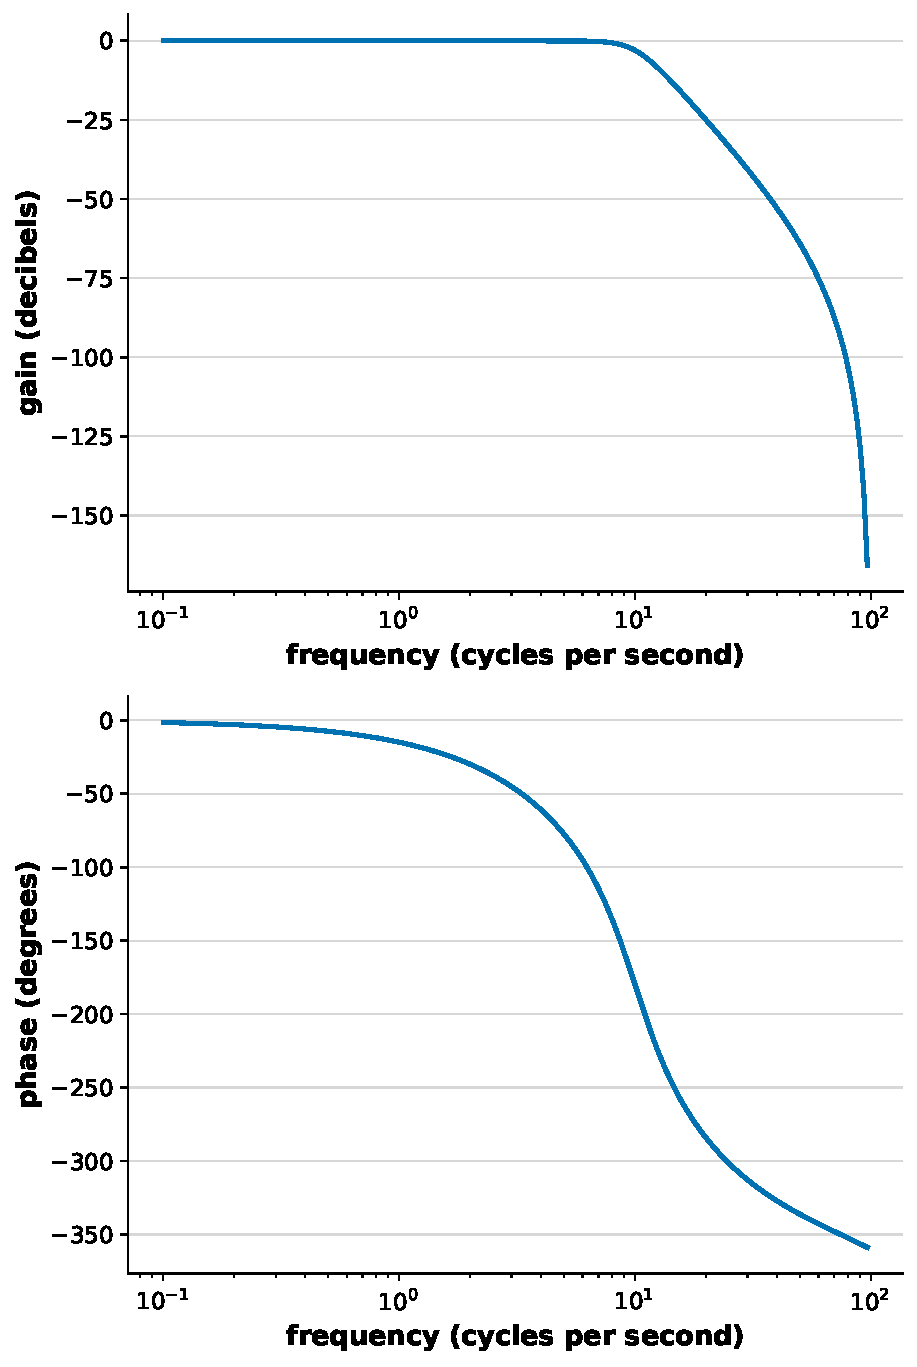
\includegraphics[width=0.72\textwidth,height=0.36\textheight,keepaspectratio]{figures/lesson26_example1_low_pass.pdf}
\captionof{figure}{Lesson 26, example 1: \code{low\_\allowbreak{}pass.\allowbreak{}png}.}
\end{minipage}\end{center}
\section*{Example 2}
A weight on a spring with a damper: push it with a force and it moves. Its output (the position) over its input (the force) is 1 / (s**2 + 0.8*s + 4). s stands for \code{\textquotedbl{}how fast it changes\textquotedbl{}}: s times the position is its speed.
\begin{lstlisting}[style=py]
import simplydata as sdata
spring = sdata.system("1 / (s**2 + 0.8*s + 4)")
spring.poles()
chart = spring.chart(show="poles and zeros")
chart.save("spring_poles.png")
spring.step_response(until=15)
chart = spring.chart(show="step", until=15)
chart.save("spring_step.png")
\end{lstlisting}
\whateachline
\begin{lineexplain}
  \item[1] Load simplydata.
  \item[2] Poles -0.4 +/- 1.96i: stable, because every pole has a negative real part. A constant force of 1 settles at 0.25. R: control::\code{tf(1,\allowbreak{} c(1,\allowbreak{} 0.\allowbreak{}8,\allowbreak{} 4))}.
  \item[3] The table of poles: damping ratio 0.2 (lightly damped), natural frequency 2.
  \item[4] The poles as x on the plane of real and imaginary parts: both lie left of the line, so the spring is stable.
  \item[5] Save it.
  \item[6] It overshoots by 52.6 \% (peak 0.3815 at time 1.58), rises in 0.60 and settles within 2 \% after 9.9. R's control::\code{step()} gives the same response.
  \item[7] The step response as a chart.
  \item[8] Save it.
\end{lineexplain}
\printedoutput{output/lesson26_example2.txt}
\begin{center}\begin{minipage}{\linewidth}\centering
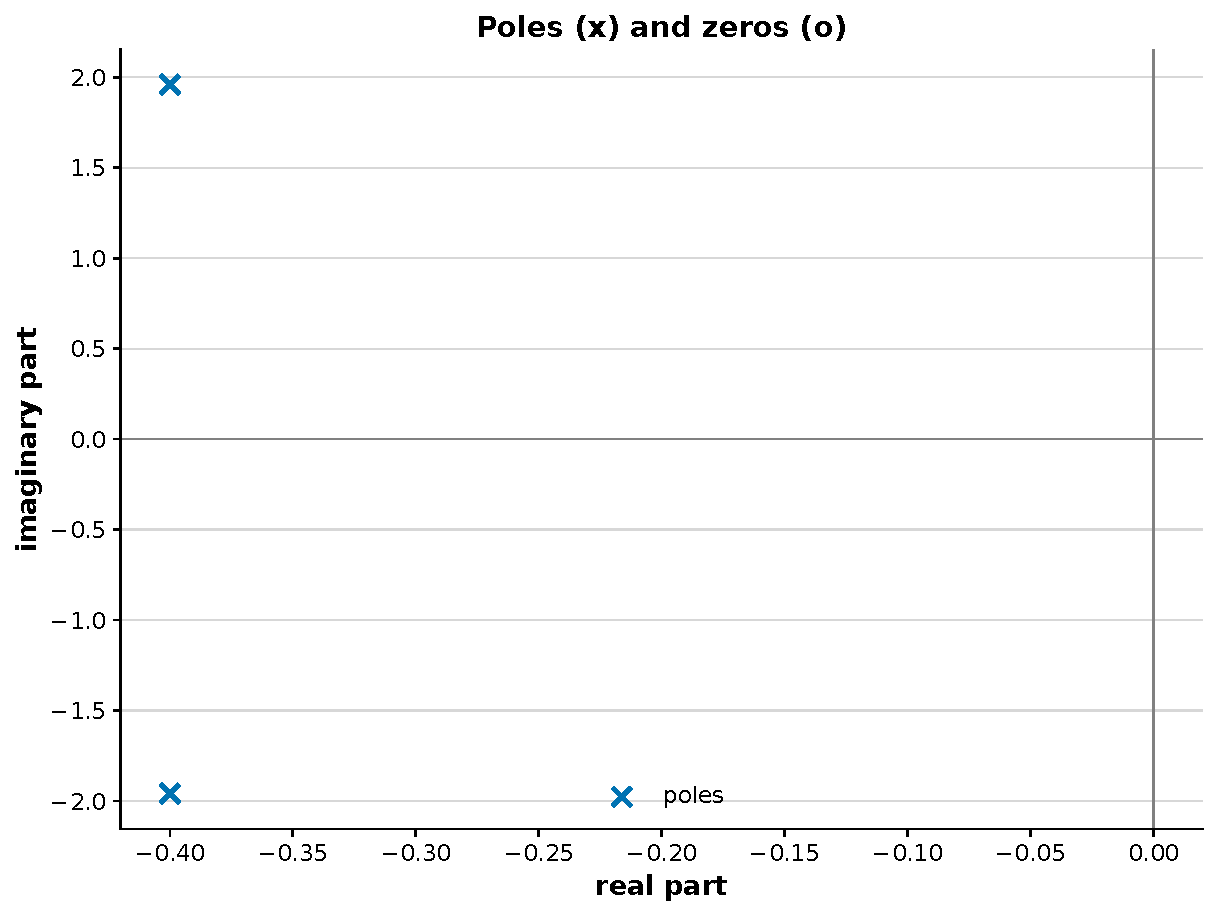
\includegraphics[width=0.48\textwidth,height=0.36\textheight,keepaspectratio]{figures/lesson26_example2_spring_poles.pdf}\hfill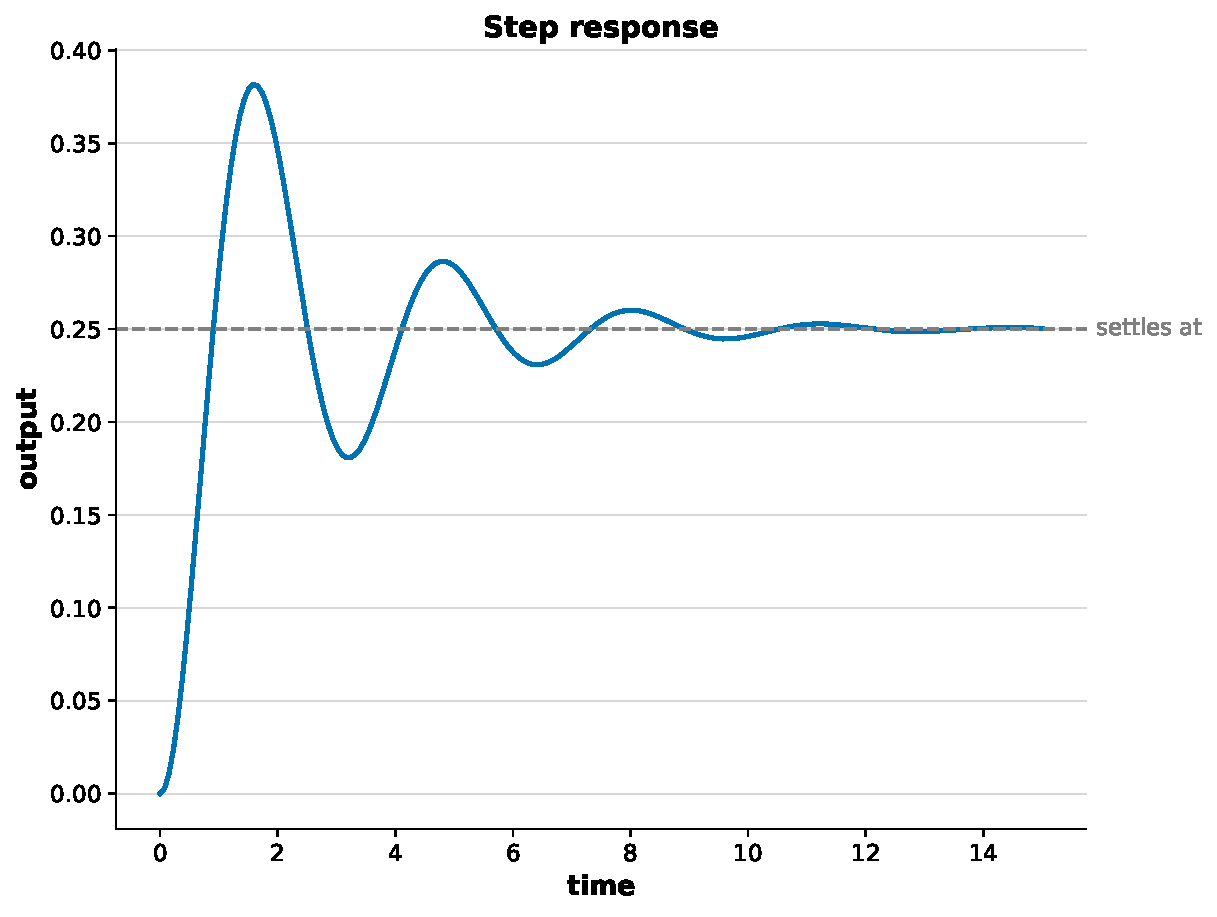
\includegraphics[width=0.48\textwidth,height=0.36\textheight,keepaspectratio]{figures/lesson26_example2_spring_step.pdf}
\captionof{figure}{Lesson 26, example 2: \code{spring\_\allowbreak{}poles.\allowbreak{}png} and \code{spring\_\allowbreak{}step.\allowbreak{}png}.}
\end{minipage}\end{center}
\section*{Example 3}
A controller measures the position, compares it with the target and pushes. This one pushes by 2 x the error plus 2 x the error added up over time: 2 * (s + 1) / s.
\begin{lstlisting}[style=py]
import simplydata as sdata
spring = sdata.system("1 / (s**2 + 0.8*s + 4)")
controller = sdata.system("2 * (s + 1) / s")
loop = controller.then(spring).with_feedback()
loop.step_response(until=30)
\end{lstlisting}
\whateachline
\begin{lineexplain}
  \item[1] Load simplydata.
  \item[2] The spring.
  \item[3] The controller.
  \item[4] The controller, then the spring, with the position fed back: (2*s + 2) / (s**3 + 0.8*s**2 + 6*s + 2), as R control::\code{feedback()}.
  \item[5] Now the position settles at the target, 1 (without the controller it settled at 0.25), with only 1.5 \% overshoot.
\end{lineexplain}
\printedoutput{output/lesson26_example3.txt}
\section*{Example 4}
More (if you want it): the frequency response says how much of each frequency gets through (the gain) and how late (the phase). The frequencies of systems are in radians per second, as R control and SciPy: 2 radians per second is 0.32 cycles per second.
\begin{lstlisting}[style=py]
import simplydata as sdata
spring = sdata.system("1 / (s**2 + 0.8*s + 4)")
spring.frequency_response(between=[0.1, 10])
chart = spring.chart(between=[0.1, 10])
chart.save("spring_bode.png")
controller = sdata.system("2 * (s + 1) / s")
controller.then(spring).frequency_response()
\end{lstlisting}
\whateachline
\begin{lineexplain}
  \item[1] Load simplydata.
  \item[2] The spring.
  \item[3] -12.02 decibels at 0.1 radians per second, -39.68 at 10; R's control::\code{bode()} gives the same.
  \item[4] The Bode chart: a peak near 2 radians per second, where the spring rings.
  \item[5] Save it.
  \item[6] The controller.
  \item[7] Before closing the loop: gain margin 18.06 decibels and phase margin 32.98 degrees. The loop could take about 8 times the gain, or 33 degrees more delay, before it stopped settling.
\end{lineexplain}
\printedoutput{output/lesson26_example4.txt}
\begin{center}\begin{minipage}{\linewidth}\centering
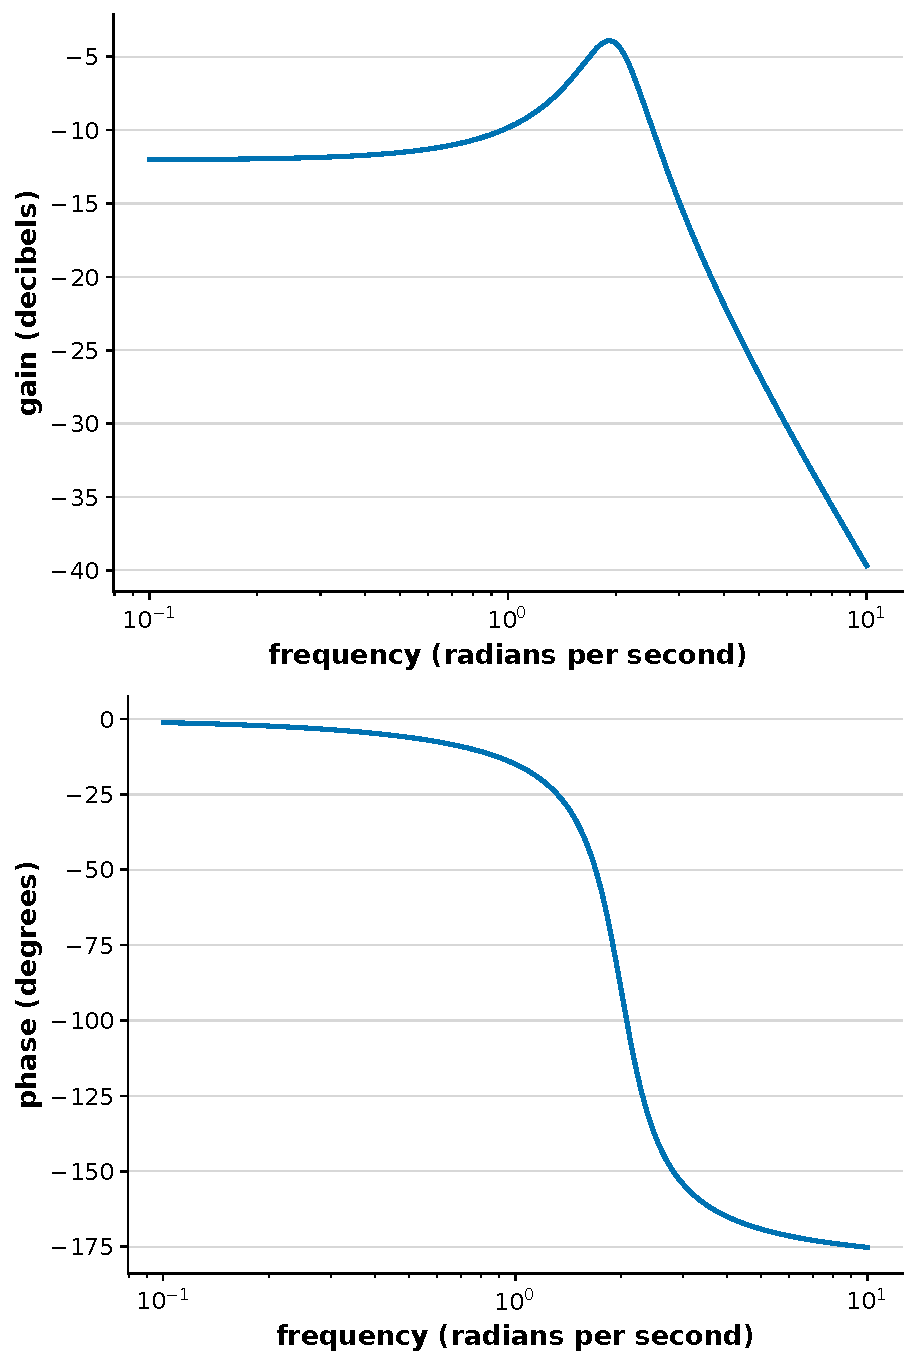
\includegraphics[width=0.72\textwidth,height=0.36\textheight,keepaspectratio]{figures/lesson26_example4_spring_bode.pdf}
\captionof{figure}{Lesson 26, example 4: \code{spring\_\allowbreak{}bode.\allowbreak{}png}.}
\end{minipage}\end{center}
\section*{Example 5}
More (if you want it): a computer reads and acts in steps. \code{in\_\allowbreak{}steps} turns the system into one that works every 0.1 seconds.
\begin{lstlisting}[style=py]
import simplydata as sdata
spring = sdata.system("1 / (s**2 + 0.8*s + 4)")
digital = spring.in_steps(time_step=0.1)
response = digital.step_response(until=15)
chart = response.start_chart()
chart.draw_lines(x="time", y="output", joined_by="steps")
chart.save("spring_in_steps.png")
\end{lstlisting}
\whateachline
\begin{lineexplain}
  \item[1] Load simplydata.
  \item[2] The spring.
  \item[3] (0.00485317*z + 0.0047253) / (z**2 - 1.8848*z + 0.923116), as R control::\code{c2d(sys,\allowbreak{} 0.\allowbreak{}1)}.
  \item[4] Almost the same answer as before: overshoot 52.7 \%, settling time 9.9.
  \item[5] The response is a table, so it can be drawn like any other.
  \item[6] Each value holds until the next step, as the computer sees it.
  \item[7] Save it.
\end{lineexplain}
\printedoutput{output/lesson26_example5.txt}
\begin{center}\begin{minipage}{\linewidth}\centering
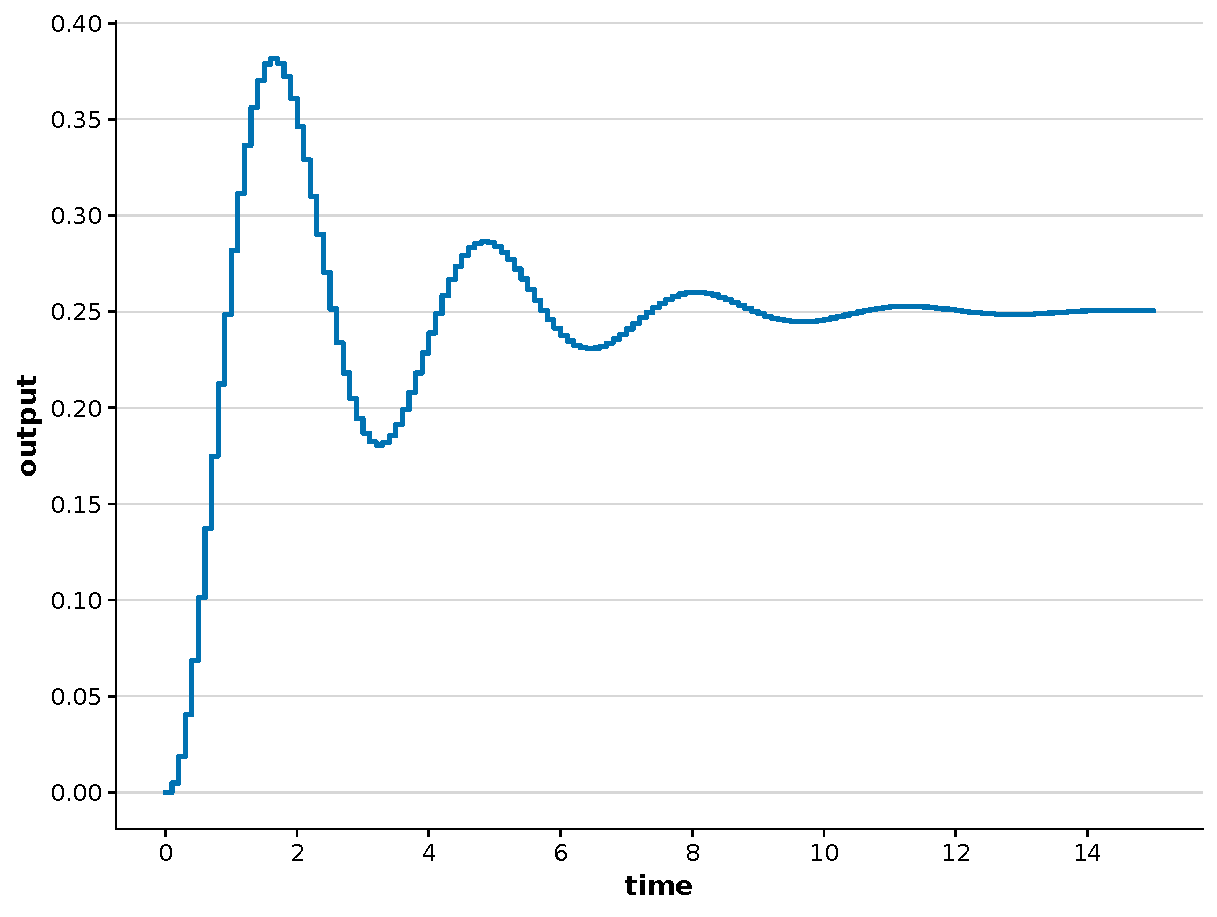
\includegraphics[width=0.72\textwidth,height=0.36\textheight,keepaspectratio]{figures/lesson26_example5_spring_in_steps.pdf}
\captionof{figure}{Lesson 26, example 5: \code{spring\_\allowbreak{}in\_\allowbreak{}steps.\allowbreak{}png}.}
\end{minipage}\end{center}
\begin{goodtoknow}
\begin{itemize}
  \item This lesson is optional: no other lesson needs it.
  \item A system can be written as a formula, as \code{numerator=} and \code{denominator=} (highest power first), as \code{poles=} and \code{zeros=}, or as matrices \code{a=}, \code{b=}, \code{c=}, \code{d=}.
  \item Frequencies of systems are in radians per second, as R control and SciPy; \code{unit=\textquotedbl{}cycles per second\textquotedbl{}} gives cycles per second. A filter from \code{sdata.\allowbreak{}frequency\_\allowbreak{}filter} is in cycles per second.
  \item R's control package has no \code{stepinfo()} or \code{margin()}: the rise time, settling time, overshoot and margins come from python-control (\code{step\_\allowbreak{}info}, \code{stability\_\allowbreak{}margins}), the Python package for control systems. Install it with pip install \code{\textquotedbl{}simplydata[systems]\textquotedbl{}}; without it the responses still come.
\end{itemize}
\end{goodtoknow}
\begin{tryit}
\begin{enumerate}
  \item Make the damper stronger: 1 / (s**2 + 2*s + 4). What happens to the overshoot?
  \item Use a controller that only pushes in proportion to the error, \code{sdata.\allowbreak{}system(\textquotedbl{}10\textquotedbl{})}. Where does the position settle?
  \item Draw the poles and zeros of the closed loop of part 3.
\end{enumerate}
Worked solutions: page~\pageref{solutions:26}, or type \code{sdata.\allowbreak{}show\_\allowbreak{}lesson(26,\allowbreak{} solutions=True)}.
\end{tryit}
\par\noindent{\small\sffamily\textbf{Words in this lesson:} \hyperref[word:sdata.frequency-filter]{\code{sdata.\allowbreak{}frequency\_\allowbreak{}filter()}}, \hyperref[word:sdata.system]{\code{sdata.\allowbreak{}system()}}, \hyperref[word:system.poles]{\code{system.\allowbreak{}poles()}}, \hyperref[word:system.chart]{\code{system.\allowbreak{}chart()}}, \hyperref[word:system.step-response]{\code{system.\allowbreak{}step\_\allowbreak{}response()}}, \hyperref[word:system.then]{\code{system.\allowbreak{}then()}}, \hyperref[word:system.with-feedback]{\code{system.\allowbreak{}with\_\allowbreak{}feedback()}}, \hyperref[word:system.frequency-response]{\code{system.\allowbreak{}frequency\_\allowbreak{}response()}}, \hyperref[word:system.in-steps]{\code{system.\allowbreak{}in\_\allowbreak{}steps()}}.\par}

\chapter{Beyond the average line: outliers}\label{lesson:27}
\begin{learnbox}
\begin{itemize}
  \item how a few rows far from the rest pull an ordinary model towards them
  \item how to give those rows less weight (robust regression, Huber's method)
  \item how \code{giving\_\allowbreak{}outliers\_\allowbreak{}less\_\allowbreak{}weight=} differs from \code{robust\_\allowbreak{}errors=}
\end{itemize}
\end{learnbox}
\section*{Example}
A least-squares line counts every row the same, so a few rows far from the rest pull it towards them. Robust regression gives those rows less weight, so they pull less.
\begin{lstlisting}[style=py]
import simplydata as sdata
table = sdata.table(sdata.get_example("school"))
table.explain("marks", using=["hours", "breakfast"])
table.explain("marks", using=["hours", "breakfast"], giving_outliers_less_weight=True)
table.explain("marks", using=["hours", "breakfast"], robust_errors=True)
\end{lstlisting}
\whateachline
\begin{lineexplain}
  \item[1] Load simplydata.
  \item[2] Pupils in 12 schools (lesson 16).
  \item[3] The ordinary model (least squares, as in lesson 16): each extra hour of study goes with about 2.8 more marks.
  \item[4] The same model with Huber's weights: rows far from the line count less. The effect of study hardly moves (2.87), and the printout lists the rows given less weight, by their row number. Say in words what that means: no few pupils decide the answer here.
  \item[5] Not the same thing: \code{robust\_\allowbreak{}errors=True} keeps the effects of the ordinary model (2.82) and only changes their standard errors, so the intervals stay right when the spread is not the same everywhere. Outliers still pull.
\end{lineexplain}
\printedoutput{output/lesson27_example1.txt}
\begin{goodtoknow}
\begin{itemize}
  \item \code{giving\_\allowbreak{}outliers\_\allowbreak{}less\_\allowbreak{}weight=True} changes the effects (rows far from the model count less); \code{robust\_\allowbreak{}errors=True} keeps the effects and changes only their standard errors. Choose by the problem: outliers, or a spread that is not the same everywhere.
  \item Huber's method resists outliers in the column you explain, not unusual values in the \code{using=} columns (far-out hours, for example). \code{table.\allowbreak{}show\_\allowbreak{}rows\_\allowbreak{}that\_\allowbreak{}pull\_\allowbreak{}model()} finds those.
  \item A row given less weight is not wrong: look at it before you decide anything. Say in your report that you used robust regression (Huber's M-estimation, as R MASS::\code{rlm()}).
\end{itemize}
\end{goodtoknow}
\begin{tryit}
\begin{enumerate}
  \item In the marks table, explain \code{\textquotedbl{}marks\textquotedbl{}} from \code{\textquotedbl{}hours\textquotedbl{}} with \code{giving\_\allowbreak{}outliers\_\allowbreak{}less\_\allowbreak{}weight=True}. Which rows get less weight?
  \item Without looking back: which option changes the effects themselves, \code{giving\_\allowbreak{}outliers\_\allowbreak{}less\_\allowbreak{}weight=} or \code{robust\_\allowbreak{}errors=}? Run both on the school table to check.
\end{enumerate}
Worked solutions: page~\pageref{solutions:27}, or type \code{sdata.\allowbreak{}show\_\allowbreak{}lesson(27,\allowbreak{} solutions=True)}.
\end{tryit}
\par\noindent{\small\sffamily\textbf{Words in this lesson:} \hyperref[word:table.explain]{\code{table.\allowbreak{}explain()}}, \hyperref[word:table.show-rows-that-pull-model]{\code{table.\allowbreak{}show\_\allowbreak{}rows\_\allowbreak{}that\_\allowbreak{}pull\_\allowbreak{}model()}}.\par}

\otherchapters

\part{Dictionary of words}\label{part:dictionary}

\unchapter{How to read the dictionary}{dictionary:how}

Each entry gives the word as you type it, what it does (in the words of \code{sdata.\allowbreak{}help(\textquotedbl{}word\textquotedbl{})}), the options you can put in its brackets and what they normally are, the library that does the work underneath, and an example you can run as it is. The same entries are in Python: \code{sdata.\allowbreak{}help(\textquotedbl{}draw\_\allowbreak{}bars\textquotedbl{})}. The words come in the same groups as \code{sdata.\allowbreak{}show\_\allowbreak{}all\_\allowbreak{}words()}; the \hyperref[index]{index of words} at the end of the book lists them A to Z.

Some entries end with a grey box, \textbf{The same underneath}. It shows the same job written in the package simplydata uses: pandas and then Polars for tables, NumPy for numbers, seaborn or matplotlib for charts, SciPy or statsmodels for statistics, and R where simplydata runs R for you. The box is for readers who know one of these packages or want to learn it; if you are learning simplydata, you can skip it. Each setting that simplydata chooses for you is marked in the code with a number, (1), (2) and so on, and explained under the code. A test runs the code in each box next to the simplydata word and checks that both give the same result, so the box cannot drift from simplydata. simplydata runs its table steps on pandas and Polars through narwhals; narwhals is only the link between the two and is not shown.

\unchapter{Chart words}{family:chart}
Steps on a chart: \code{chart = sdata.chart(table)}, then \code{chart.draw\_bars(...)}. Words that start with \code{sdata.} are called on simplydata itself, and words that end in \code{=} are options inside a chart step.
\unsection{Start, show and save}{group:Start-show-and-save}
\wordentry{sdata.chart()}{word:sdata.chart}
Start a chart. \code{sdata.\allowbreak{}chart(sdata.\allowbreak{}get\_\allowbreak{}example(\textquotedbl{}marks\textquotedbl{}))}

\codeline{sdata.chart(table)}\enspace a pandas or Polars table, like \code{sdata.\allowbreak{}get\_\allowbreak{}example(\textquotedbl{}marks\textquotedbl{})}\\
\codeline{sdata.chart(\textquotedbl{}my\_file.xlsx\textquotedbl{})}\enspace your own file (Excel, CSV, TSV, Parquet, JSON)\\
\codeline{sdata.chart(\textquotedbl{}my\_file.xlsx\textquotedbl{}, sheet=\textquotedbl{}2026\textquotedbl{}) one sheet of an Excel file}\\
\codeline{sdata.chart()}\enspace no table: give lists to each step instead\\
\codeline{fast=True}\enspace always use the fast engine (Polars) to read the file

\wordfield{Options}{}\par\nopagebreak
\begin{optiontable}
\code{data=} & \\
\code{sheet=} & \\
\code{fast=} & normally \code{False}\\
\end{optiontable}

\wordfield{Underneath}{pandas reads the file (Polars for big files); the chart is drawn with matplotlib and seaborn}
\wordfield{Example you can run}{}\par\nopagebreak
\begin{lstlisting}[style=py]
import simplydata as sdata
marks = sdata.get_example("marks")
chart = sdata.chart(marks)
chart.draw_dots(x="hours", y="marks")
chart.save("my_chart.png")
\end{lstlisting}
\wordentry{sdata.get\_example()}{word:sdata.get-example}
A small made-up table to practise with. \code{sdata.\allowbreak{}get\_\allowbreak{}example(\textquotedbl{}marks\textquotedbl{})}

\codeline{sdata.get\_example() with no name lists every table and its columns.}\\
The tables are: marks, weather, fruit, growth, sensor, visitors, river, shop, school, meadow, trial, clinic, island. \code{\textquotedbl{}shop\textquotedbl{}} has empty cells and a column of dates to practise with; \code{\textquotedbl{}school\textquotedbl{}} has empty cells too.

\wordfield{Options}{}\par\nopagebreak
\begin{optiontable}
\code{name=} & \\
\end{optiontable}

\wordfield{Underneath}{pandas (\code{read\_\allowbreak{}csv} of a small file inside simplydata)}
\wordfield{Example you can run}{}\par\nopagebreak
\begin{lstlisting}[style=py]
import simplydata as sdata
sdata.get_example()
marks = sdata.get_example("marks")
print(marks)
\end{lstlisting}
\wordentry{chart.show()}{word:show}
Show the chart in a window. \code{chart.\allowbreak{}show()}

In Jupyter, VS Code and Spyder charts appear by themselves.

\wordfield{Options}{none: just write the empty brackets.}

\wordfield{Good to know}{Not the same as the \code{show=} option inside \code{draw\_\allowbreak{}bars} and \code{draw\_\allowbreak{}lines}: for that, type \code{sdata.\allowbreak{}help(\textquotedbl{}show=\textquotedbl{})}.}

\wordfield{Underneath}{matplotlib (pyplot.show)}
\wordfield{Example you can run}{}\par\nopagebreak
\begin{lstlisting}[style=py]
import simplydata as sdata
marks = sdata.get_example("marks")
chart = sdata.chart(marks)
chart.draw_bars(x="name", y="marks")
chart.show()
chart.save("marks.png")
\end{lstlisting}
\wordentry{chart.save()}{word:save}
Save the chart. \code{chart.\allowbreak{}save(\textquotedbl{}marks.\allowbreak{}png\textquotedbl{})} or \code{chart.\allowbreak{}save(\textquotedbl{}marks.\allowbreak{}tif\textquotedbl{},\allowbreak{} resolution=600)}

The end of the file name decides the format: \code{\textquotedbl{}marks.\allowbreak{}png\textquotedbl{}}, \code{\textquotedbl{}marks.\allowbreak{}pdf\textquotedbl{}}. \code{resolution=} is the sharpness in dots per inch (dpi); normally 300.

\wordfield{Options}{}\par\nopagebreak
\begin{optiontable}
\code{file\_\allowbreak{}name} & needed\\
\code{quality=} & normally \code{\textquotedbl{}normal\textquotedbl{}}\\
\code{resolution=} & \\
\code{dpi=} & \\
\end{optiontable}

\wordfield{Good to know}{File types: \code{.\allowbreak{}png} (a picture), \code{.\allowbreak{}pdf} and \code{.\allowbreak{}svg} (sharp at any size, good for printing), \code{.\allowbreak{}jpg}, \code{.\allowbreak{}tif}, and \code{.\allowbreak{}gif} for animations. \code{resolution=} is how sharp a picture is, in dots per inch (dpi): 300 is normal, journals often ask for 300 or 600 (\code{dpi=} means the same). \code{quality=\textquotedbl{}high\textquotedbl{}} is the same as \code{resolution=600}. \code{.\allowbreak{}tif} files are compressed without losing anything. To choose the size of the file in cm, mm or pixels, use \code{chart.\allowbreak{}set\_\allowbreak{}size()} first.}

\wordfield{Underneath}{matplotlib (Figure.savefig); Pillow writes \code{.\allowbreak{}gif} animations}
\wordfield{Example you can run}{}\par\nopagebreak
\begin{lstlisting}[style=py]
import simplydata as sdata
marks = sdata.get_example("marks")
chart = sdata.chart(marks)
chart.draw_bars(x="name", y="marks")
chart.save("marks.png")
chart.save("marks.pdf")
chart.save("marks.tif", resolution=600)
\end{lstlisting}
\unsection{Chart types}{group:Chart-types}
\wordentry{chart.draw\_bars()}{word:draw-bars}
Bars. \code{chart.\allowbreak{}draw\_\allowbreak{}bars(x=\textquotedbl{}name\textquotedbl{},\allowbreak{} y=\textquotedbl{}marks\textquotedbl{})} (with \code{sdata.\allowbreak{}get\_\allowbreak{}example(\textquotedbl{}marks\textquotedbl{})})

\code{colour=\textquotedbl{}class\textquotedbl{}} gives each group its own colour, or \code{colour=\textquotedbl{}blue\textquotedbl{}} one colour. \code{show=} says what each bar stands for when a group has many rows: \code{\textquotedbl{}average\textquotedbl{}} (default), \code{\textquotedbl{}median\textquotedbl{}}, \code{\textquotedbl{}total\textquotedbl{}}, \code{\textquotedbl{}count\textquotedbl{}}, \code{\textquotedbl{}smallest\textquotedbl{}}, \code{\textquotedbl{}biggest\textquotedbl{}} or \code{\textquotedbl{}standard deviation\textquotedbl{}}. \code{error=\textquotedbl{}standard deviation\textquotedbl{}}, \code{\textquotedbl{}standard error\textquotedbl{}} or \code{\textquotedbl{}confidence interval\textquotedbl{}} adds error bars (with \code{show=\textquotedbl{}average\textquotedbl{}}); a line says which one was drawn. \code{stacked=True} puts groups on top of each other; \code{sideways=True} lays bars down. \code{transparency=0.\allowbreak{}5} makes them half see-through (0 is solid).

\wordfield{Options}{}\par\nopagebreak
\begin{optiontable}
\code{x=} & \\
\code{y=} & \\
\code{colour=} & \\
\code{show=} & normally \code{\textquotedbl{}average\textquotedbl{}}\\
\code{error=} & \\
\code{stacked=} & normally \code{False}\\
\code{sideways=} & normally \code{False}\\
\code{transparency=} & \\
\end{optiontable}

\wordfield{Underneath}{seaborn \code{barplot()}}
\wordfield{Example you can run}{}\par\nopagebreak
\begin{lstlisting}[style=py]
import simplydata as sdata
marks = sdata.get_example("marks")
chart = sdata.chart(marks)
chart.draw_bars(x="name", y="marks", colour="class")
chart.rotate_labels_x()
chart.save("draw_bars.png")
\end{lstlisting}
\begin{center}\begin{minipage}{\linewidth}\centering
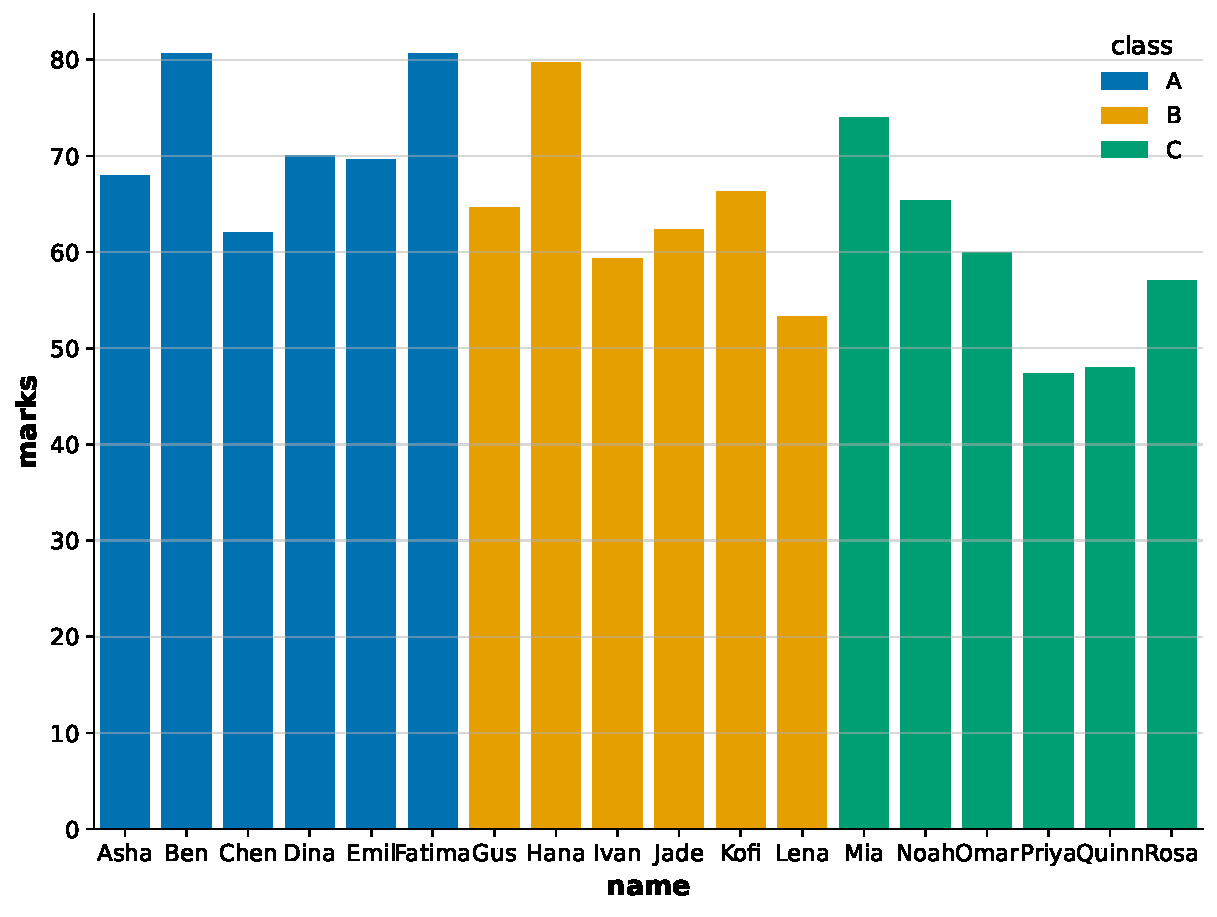
\includegraphics[width=0.52\textwidth,height=0.26\textheight,keepaspectratio]{figures/underneath_draw_bars.pdf}
\captionof*{figure}{The chart simplydata draws. The code below draws the same bars, without simplydata's paper look.}
\end{minipage}\end{center}
\needspace{10\baselineskip}\begin{underneathbox}{\libbadge{seaborn}}
\underlib{seaborn}
\begin{lstlisting}[style=under]
import matplotlib.pyplot as plt
import seaborn as sns
df = sdata.get_example("marks")
fig, ax = plt.subplots()
# draw_bars(x="name", y="marks", colour="class")
sns.barplot(df, x="name", y="marks", hue="class",
            errorbar=None, ax=ax)           # (1)
\end{lstlisting}
\undertext{\textbf{simplydata chooses}}
\undertext{(1) simplydata draws no error bars unless you ask (\code{error=}); seaborn's own default draws a bootstrap 95 \% interval on each bar.}
\undertext{Each bar is the average of its rows, as in seaborn. simplydata also gives the chart its paper look (fonts, colours, no top and right lines); that is left out here.}
\undertext{\textit{Checked:} a test runs both and compares the bars, which bars share a colour, the lines, the axis labels, the tick labels, the legend and the axis ranges (the chart's data, not its pixels).}
\end{underneathbox}
\wordentry{chart.draw\_lines()}{word:draw-lines}
Lines. \code{chart.\allowbreak{}draw\_\allowbreak{}lines(x=\textquotedbl{}month\textquotedbl{},\allowbreak{} y=\textquotedbl{}temperature\textquotedbl{},\allowbreak{} colour=\textquotedbl{}city\textquotedbl{})} (with \code{sdata.\allowbreak{}get\_\allowbreak{}example(\textquotedbl{}weather\textquotedbl{})})

\code{colour=\textquotedbl{}city\textquotedbl{}} draws one line per group. \code{with\_\allowbreak{}dots=True} marks each point. \code{dashed=True} draws a dashed line. \code{show=} works as in bars (not \code{\textquotedbl{}count\textquotedbl{}}). \code{error=\textquotedbl{}standard deviation\textquotedbl{}}, \code{\textquotedbl{}standard error\textquotedbl{}} or \code{\textquotedbl{}confidence interval\textquotedbl{}} adds a shaded band; a line says which one was drawn. \code{thickness=3} draws thicker lines (normal is 2, in points); \code{transparency=0.\allowbreak{}5} makes them half see-through (0 is solid). \code{joined\_\allowbreak{}by=} says how the points are joined, as in \code{table.\allowbreak{}values\_\allowbreak{}at()}: \code{\textquotedbl{}straight lines\textquotedbl{}} (normal), \code{\textquotedbl{}smooth curve\textquotedbl{}} (natural cubic spline), \code{\textquotedbl{}curve without overshoot\textquotedbl{}} (PCHIP), \code{\textquotedbl{}steps\textquotedbl{}} (each value stays until the next point), \code{\textquotedbl{}nearest\textquotedbl{}}; experts: \code{\textquotedbl{}akima\textquotedbl{}}, \code{\textquotedbl{}makima\textquotedbl{}}, \code{\textquotedbl{}not-a-knot\textquotedbl{}}, \code{\textquotedbl{}periodic\textquotedbl{}}. Curves need numbers on x and y.

\wordfield{Options}{}\par\nopagebreak
\begin{optiontable}
\code{x=} & \\
\code{y=} & \\
\code{colour=} & \\
\code{show=} & normally \code{\textquotedbl{}average\textquotedbl{}}\\
\code{error=} & \\
\code{with\_\allowbreak{}dots=} & normally \code{False}\\
\code{dashed=} & normally \code{False}\\
\code{thickness=} & \\
\code{transparency=} & \\
\code{joined\_\allowbreak{}by=} & normally \code{\textquotedbl{}straight lines\textquotedbl{}}\\
\end{optiontable}

\wordfield{Underneath}{seaborn (lineplot); SciPy (interpolate) for \code{joined\_\allowbreak{}by=} curves}
\wordfield{Example you can run}{}\par\nopagebreak
\begin{lstlisting}[style=py]
import simplydata as sdata
weather = sdata.get_example("weather")
chart = sdata.chart(weather)
chart.draw_lines(x="month", y="temperature", colour="city", with_dots=True)
chart.save("draw_lines.png")
\end{lstlisting}
\wordentry{chart.draw\_dots()}{word:draw-dots}
Dots (a scatter chart). \code{chart.\allowbreak{}draw\_\allowbreak{}dots(x=\textquotedbl{}hours\textquotedbl{},\allowbreak{} y=\textquotedbl{}marks\textquotedbl{})} (with \code{sdata.\allowbreak{}get\_\allowbreak{}example(\textquotedbl{}marks\textquotedbl{})})

\code{colour=\textquotedbl{}class\textquotedbl{}} colours dots by group. \code{size=\textquotedbl{}height\textquotedbl{}} makes dots bigger for bigger values, or \code{size=10} makes all dots that big. \code{shape=\textquotedbl{}subject\textquotedbl{}} gives each group a shape. \code{transparency=0.\allowbreak{}5} makes dots half see-through, so dots on top of each other show. With \code{colour=} a number column and \code{chart.\allowbreak{}use\_\allowbreak{}colour\_\allowbreak{}scale(.\allowbreak{}.\allowbreak{}.\allowbreak{})}, dots get a smooth colour scale and a colour bar.

\wordfield{Options}{}\par\nopagebreak
\begin{optiontable}
\code{x=} & \\
\code{y=} & \\
\code{colour=} & \\
\code{size=} & \\
\code{shape=} & \\
\code{transparency=} & \\
\end{optiontable}

\wordfield{Underneath}{seaborn \code{scatterplot()}}
\wordfield{Example you can run}{}\par\nopagebreak
\begin{lstlisting}[style=py]
import simplydata as sdata
marks = sdata.get_example("marks")
chart = sdata.chart(marks)
chart.draw_dots(x="hours", y="marks", colour="class", size="height")
chart.save("draw_dots.png")
\end{lstlisting}
\begin{center}\begin{minipage}{\linewidth}\centering
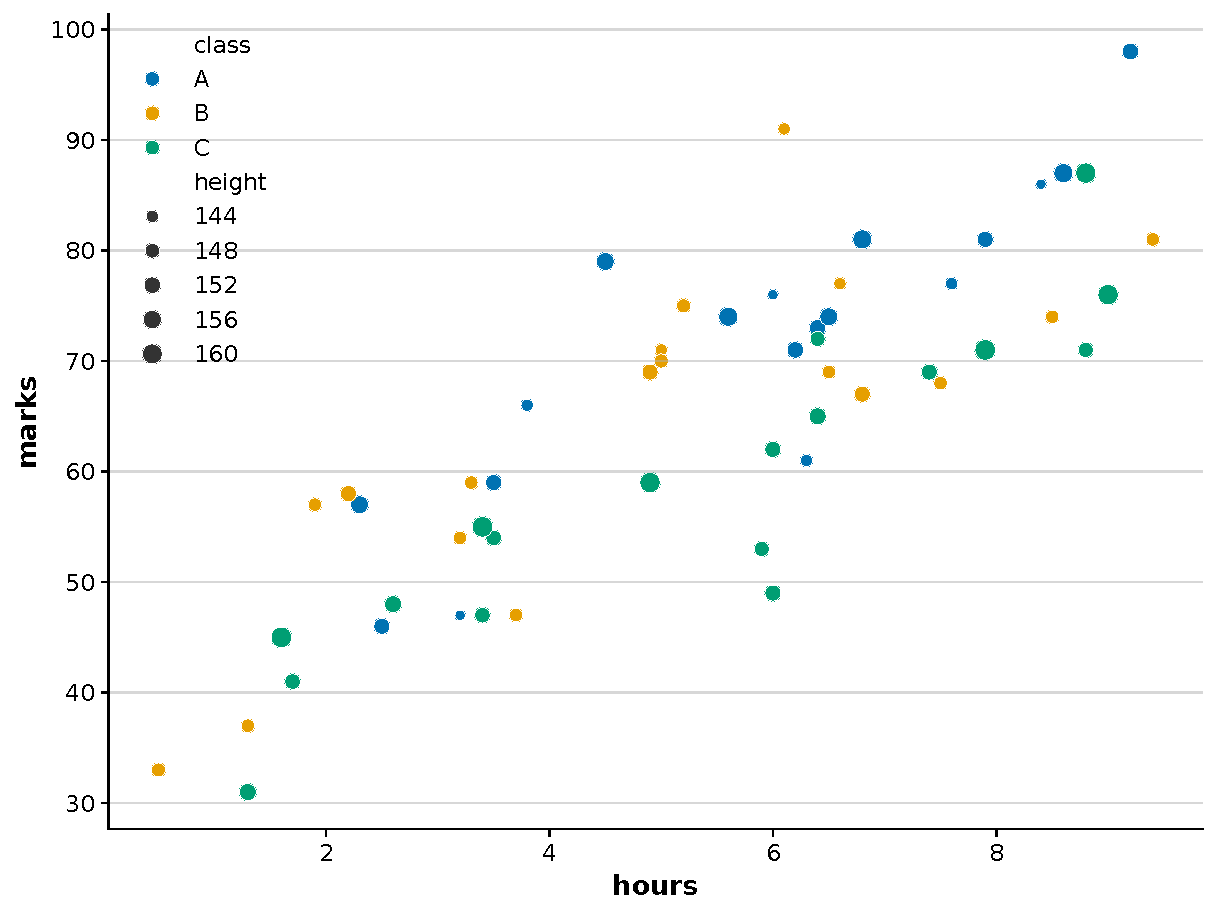
\includegraphics[width=0.52\textwidth,height=0.26\textheight,keepaspectratio]{figures/underneath_draw_dots.pdf}
\captionof*{figure}{The chart simplydata draws. The code below draws the same dots, without simplydata's paper look.}
\end{minipage}\end{center}
\needspace{10\baselineskip}\begin{underneathbox}{\libbadge{seaborn}}
\underlib{seaborn}
\begin{lstlisting}[style=under]
import matplotlib.pyplot as plt
import seaborn as sns
df = sdata.get_example("marks")
fig, ax = plt.subplots()
# draw_dots(x="hours", y="marks", colour="class", size="height")
sns.scatterplot(df, x="hours", y="marks", hue="class",
                size="height", ax=ax)
\end{lstlisting}
\undertext{simplydata's paper look draws every dot a little bigger; the sizes keep the same proportions. simplydata also gives the chart its paper look (fonts, colours, no top and right lines); that is left out here.}
\undertext{\textit{Checked:} a test runs both and compares the dots, the dot sizes, which dots share a colour, the axis labels, the legend and the axis ranges (the chart's data, not its pixels).}
\end{underneathbox}
\wordentry{chart.draw\_area()}{word:draw-area}
A line with the space under it coloured in.\\
\codeline{chart.draw\_area(x=\textquotedbl{}year\textquotedbl{}, y=\textquotedbl{}population\textquotedbl{}, colour=\textquotedbl{}country\textquotedbl{}) (with sdata.get\_example(\textquotedbl{}growth\textquotedbl{}))}

\code{colour=\textquotedbl{}country\textquotedbl{}} gives each group its own area; \code{stacked=True} piles the groups on top of each other, so the top edge shows the total. \code{transparency=0.\allowbreak{}3} sets how see-through the coloured space is (0 is solid); \code{thickness=3} makes its top line thicker.

\wordfield{Options}{}\par\nopagebreak
\begin{optiontable}
\code{x=} & \\
\code{y=} & \\
\code{colour=} & \\
\code{stacked=} & normally \code{False}\\
\code{transparency=} & \\
\code{thickness=} & \\
\end{optiontable}

\wordfield{Underneath}{matplotlib (\code{fill\_\allowbreak{}between}, or stackplot with \code{stacked=True})}
\wordfield{Example you can run}{}\par\nopagebreak
\begin{lstlisting}[style=py]
import simplydata as sdata
growth = sdata.get_example("growth")
chart = sdata.chart(growth)
chart.draw_area(x="year", y="population", colour="country", stacked=True)
chart.save("draw_area.png")
\end{lstlisting}
\wordentry{chart.draw\_histogram()}{word:draw-histogram}
Bars that count how many values fall in each range. \code{chart.\allowbreak{}draw\_\allowbreak{}histogram(x=\textquotedbl{}marks\textquotedbl{},\allowbreak{} with\_\allowbreak{}bins=10)} (with \code{sdata.\allowbreak{}get\_\allowbreak{}example(\textquotedbl{}marks\textquotedbl{})})

\code{with\_\allowbreak{}bins=} is how many bars (normally 10), or a list of where each bar starts and ends; \code{bin\_\allowbreak{}width=5} makes every bar 5 wide instead. \code{show=} is what the height of a bar means: \code{\textquotedbl{}count\textquotedbl{}} (normal), \code{\textquotedbl{}percent\textquotedbl{}} (of the values) or \code{\textquotedbl{}density\textquotedbl{}} (the bars have an area of 1, to compare with a density curve). \code{colour=\textquotedbl{}class\textquotedbl{}} draws one see-through histogram per group; with \code{show=\textquotedbl{}percent\textquotedbl{}} or \code{\textquotedbl{}density\textquotedbl{}} each group is worked out on its own. \code{stacked=True} piles the groups on top of each other instead (then the whole stack makes 100 \%). \code{steps=True} draws only the outline, as steps; \code{cumulative=True} adds up from the left, so each bar counts the values up to its right edge. \code{transparency=0.\allowbreak{}5} makes the bars half see-through; \code{thickness=} sets the outline width.

\wordfield{Options}{}\par\nopagebreak
\begin{optiontable}
\code{x=} & \\
\code{with\_\allowbreak{}bins=} & \\
\code{colour=} & \\
\code{show=} & normally \code{\textquotedbl{}count\textquotedbl{}}\\
\code{stacked=} & normally \code{False}\\
\code{steps=} & normally \code{False}\\
\code{cumulative=} & normally \code{False}\\
\code{bin\_\allowbreak{}width=} & \\
\code{transparency=} & \\
\code{thickness=} & \\
\end{optiontable}

\wordfield{Underneath}{seaborn \code{histplot()}}
\wordfield{Example you can run}{}\par\nopagebreak
\begin{lstlisting}[style=py]
import simplydata as sdata
marks = sdata.get_example("marks")
chart = sdata.chart(marks)
chart.draw_histogram(x="marks", with_bins=10)
chart.save("draw_histogram.png")
\end{lstlisting}
\begin{center}\begin{minipage}{\linewidth}\centering
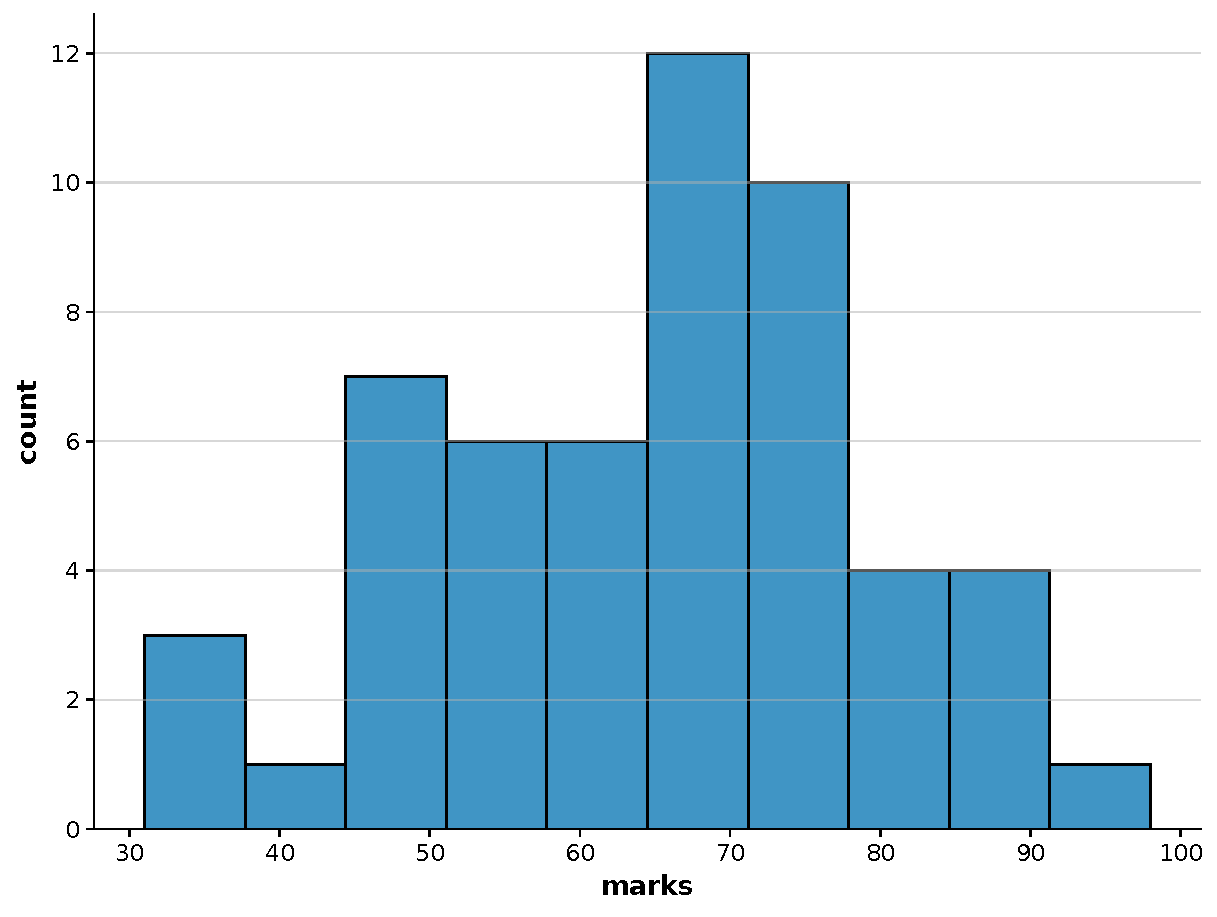
\includegraphics[width=0.52\textwidth,height=0.26\textheight,keepaspectratio]{figures/underneath_draw_histogram.pdf}
\captionof*{figure}{The chart simplydata draws. The code below draws the same bars, without simplydata's paper look.}
\end{minipage}\end{center}
\needspace{10\baselineskip}\begin{underneathbox}{\libbadge{seaborn}}
\underlib{seaborn}
\begin{lstlisting}[style=under]
import matplotlib.pyplot as plt
import seaborn as sns
df = sdata.get_example("marks")
fig, ax = plt.subplots()
# draw_histogram(x="marks")
sns.histplot(df, x="marks", bins=10, ax=ax)   # (1)
\end{lstlisting}
\undertext{\textbf{simplydata chooses}}
\undertext{(1) simplydata makes 10 bins unless you say \code{with\_\allowbreak{}bins=}; seaborn's own default chooses the number of bins from the data.}
\undertext{simplydata writes the y label in small letters (count). simplydata also gives the chart its paper look (fonts, colours, no top and right lines); that is left out here.}
\undertext{\textit{Checked:} a test runs both and compares the bars, the tick labels and the axis ranges (the chart's data, not its pixels).}
\end{underneathbox}
\wordentry{chart.draw\_boxes()}{word:draw-boxes}
Boxes that show the middle half of the values and the median.\\
\codeline{chart.draw\_boxes(x=\textquotedbl{}class\textquotedbl{}, y=\textquotedbl{}marks\textquotedbl{}) (with sdata.get\_example(\textquotedbl{}marks\textquotedbl{}))}

The line in the box is the median, the box holds the middle half of the values, the whiskers reach the rest, and lone dots are values far away from the others. \code{transparency=0.\allowbreak{}5} makes the boxes half see-through; \code{thickness=} sets the width of their lines.

\wordfield{Options}{}\par\nopagebreak
\begin{optiontable}
\code{x=} & \\
\code{y=} & \\
\code{colour=} & \\
\code{transparency=} & \\
\code{thickness=} & \\
\end{optiontable}

\wordfield{Underneath}{seaborn (boxplot)}
\wordfield{Example you can run}{}\par\nopagebreak
\begin{lstlisting}[style=py]
import simplydata as sdata
marks = sdata.get_example("marks")
chart = sdata.chart(marks)
chart.draw_boxes(x="class", y="marks")
chart.save("draw_boxes.png")
\end{lstlisting}
\wordentry{chart.draw\_violins()}{word:draw-violins}
Shapes that are wide where many values are. \code{chart.\allowbreak{}draw\_\allowbreak{}violins(x=\textquotedbl{}class\textquotedbl{},\allowbreak{} y=\textquotedbl{}marks\textquotedbl{})} (with \code{sdata.\allowbreak{}get\_\allowbreak{}example(\textquotedbl{}marks\textquotedbl{})})

Each violin stops at the smallest and the largest value; the small box inside shows the middle half of the values. \code{transparency=0.\allowbreak{}5} makes the violins half see-through; \code{thickness=} sets the width of their lines.

\wordfield{Options}{}\par\nopagebreak
\begin{optiontable}
\code{x=} & \\
\code{y=} & \\
\code{colour=} & \\
\code{transparency=} & \\
\code{thickness=} & \\
\end{optiontable}

\wordfield{Underneath}{seaborn (violinplot)}
\wordfield{Example you can run}{}\par\nopagebreak
\begin{lstlisting}[style=py]
import simplydata as sdata
marks = sdata.get_example("marks")
chart = sdata.chart(marks)
chart.draw_violins(x="subject", y="marks")
chart.save("draw_violins.png")
\end{lstlisting}
\wordentry{chart.draw\_heatmap()}{word:draw-heatmap}
A grid of coloured squares, one colour for each number.\\
\codeline{chart.draw\_heatmap(x=\textquotedbl{}month\textquotedbl{}, y=\textquotedbl{}city\textquotedbl{}, value=\textquotedbl{}rain\textquotedbl{}, with\_numbers=True) (with sdata.get\_example(\textquotedbl{}weather\textquotedbl{}))}

With no columns named, every number column of the table is used (rows are the table's rows): \code{chart.\allowbreak{}draw\_\allowbreak{}heatmap(with\_\allowbreak{}numbers=True)}. \code{with\_\allowbreak{}numbers=True} writes the number in each square. \code{cluster=True} puts similar rows and columns next to each other and draws a tree of how alike they are.\\
\codeline{chart.use\_colour\_scale(...) chooses the colours. transparency=0.3 lets grid lines show through.}

\wordfield{Options}{}\par\nopagebreak
\begin{optiontable}
\code{x=} & \\
\code{y=} & \\
\code{value=} & \\
\code{with\_\allowbreak{}numbers=} & normally \code{False}\\
\code{cluster=} & normally \code{False}\\
\code{transparency=} & \\
\end{optiontable}

\wordfield{Underneath}{seaborn (heatmap); SciPy (scipy.cluster.hierarchy) for \code{cluster=True}}
\wordfield{Example you can run}{}\par\nopagebreak
\begin{lstlisting}[style=py]
import simplydata as sdata
weather = sdata.get_example("weather")
chart = sdata.chart(weather)
chart.draw_heatmap(x="month", y="city", value="rain", with_numbers=True)
chart.save("draw_heatmap.png")
\end{lstlisting}
\wordentry{chart.draw\_pie()}{word:draw-pie}
A circle cut into slices, one slice per group. \code{chart.\allowbreak{}draw\_\allowbreak{}pie(labels=\textquotedbl{}fruit\textquotedbl{},\allowbreak{} values=\textquotedbl{}count\textquotedbl{})} (with \code{sdata.\allowbreak{}get\_\allowbreak{}example(\textquotedbl{}fruit\textquotedbl{})})

Without \code{values=} each slice shows how many rows have that label. \code{transparency=0.\allowbreak{}3} makes the slices a little see-through (0 is solid).

\wordfield{Options}{}\par\nopagebreak
\begin{optiontable}
\code{labels=} & \\
\code{values=} & \\
\code{transparency=} & \\
\end{optiontable}

\wordfield{Underneath}{matplotlib (Axes.pie)}
\wordfield{Example you can run}{}\par\nopagebreak
\begin{lstlisting}[style=py]
import simplydata as sdata
fruit = sdata.get_example("fruit")
chart = sdata.chart(fruit)
chart.draw_pie(labels="fruit", values="count")
chart.save("draw_pie.png")
\end{lstlisting}
\wordentry{chart.draw\_polar()}{word:draw-polar}
Dots on a round chart: how far round, and how far out.\\
\codeline{chart.draw\_polar(angle=\textquotedbl{}wind\_direction\textquotedbl{}, distance=\textquotedbl{}wind\_speed\textquotedbl{}, colour=\textquotedbl{}city\textquotedbl{}) (with sdata.get\_example(\textquotedbl{}weather\textquotedbl{}))}

Angles are in degrees (a full turn is 360), going round from the right, the way maths measures angles. Use \code{degrees=False} if your angles are in radians. \code{transparency=0.\allowbreak{}5} makes them half see-through (0 is solid).

\wordfield{Options}{}\par\nopagebreak
\begin{optiontable}
\code{angle=} & \\
\code{distance=} & \\
\code{colour=} & \\
\code{degrees=} & normally \code{True}\\
\code{transparency=} & \\
\end{optiontable}

\wordfield{Underneath}{matplotlib (polar axes)}
\wordfield{Example you can run}{}\par\nopagebreak
\begin{lstlisting}[style=py]
import simplydata as sdata
weather = sdata.get_example("weather")
chart = sdata.chart(weather)
chart.draw_polar(angle="wind_direction", distance="wind_speed", colour="city")
chart.save("draw_polar.png")
\end{lstlisting}
\wordentry{chart.draw\_contour()}{word:draw-contour}
A map where each colour band joins places with the same height.\\
\codeline{chart.draw\_contour(x=\textquotedbl{}east\textquotedbl{}, y=\textquotedbl{}north\textquotedbl{}, z=\textquotedbl{}height\textquotedbl{}) (with sdata.get\_example(\textquotedbl{}island\textquotedbl{}))}

\code{z=} is the height (or depth, or temperature). The points can be a full grid or scattered; scattered points are joined up with straight lines in between. \code{filled=False} draws only the lines, with their numbers written on them.\\
\codeline{chart.use\_colour\_scale(...) chooses the colours (and steps= the bands).}\\
\code{transparency=0.\allowbreak{}3} lets what is under it show through; \code{thickness=} sets the width of the lines.

\wordfield{Options}{}\par\nopagebreak
\begin{optiontable}
\code{x=} & \\
\code{y=} & \\
\code{z=} & \\
\code{filled=} & normally \code{True}\\
\code{transparency=} & \\
\code{thickness=} & \\
\end{optiontable}

\wordfield{Underneath}{matplotlib (contourf); SciPy (interpolate.griddata) for scattered points}
\wordfield{Example you can run}{}\par\nopagebreak
\begin{lstlisting}[style=py]
import simplydata as sdata
island = sdata.get_example("island")
chart = sdata.chart(island)
chart.draw_contour(x="east", y="north", z="height")
chart.save("draw_contour.png")
\end{lstlisting}
\wordentry{chart.draw\_surface()}{word:draw-surface}
A 3D landscape: \code{z=} is how high the ground is.\\
\codeline{chart.draw\_surface(x=\textquotedbl{}east\textquotedbl{}, y=\textquotedbl{}north\textquotedbl{}, z=\textquotedbl{}height\textquotedbl{}) (with sdata.get\_example(\textquotedbl{}island\textquotedbl{}))}

The points can be a full grid or scattered; scattered points are joined up.\\
\codeline{chart.use\_colour\_scale(...) chooses the colours. transparency=0.3 makes it a little see-through.}

\wordfield{Options}{}\par\nopagebreak
\begin{optiontable}
\code{x=} & \\
\code{y=} & \\
\code{z=} & \\
\code{transparency=} & \\
\end{optiontable}

\wordfield{Underneath}{matplotlib (mplot3d \code{plot\_\allowbreak{}surface}); SciPy (interpolate.griddata) for scattered points}
\wordfield{Example you can run}{}\par\nopagebreak
\begin{lstlisting}[style=py]
import simplydata as sdata
island = sdata.get_example("island")
chart = sdata.chart(island)
chart.draw_surface(x="east", y="north", z="height")
chart.save("draw_surface.png")
\end{lstlisting}
\wordentry{chart.draw\_dots\_3d()}{word:draw-dots-3d}
Dots floating in a 3D box. \code{chart.\allowbreak{}draw\_\allowbreak{}dots\_\allowbreak{}3d(x=\textquotedbl{}hours\textquotedbl{},\allowbreak{} y=\textquotedbl{}height\textquotedbl{},\allowbreak{} z=\textquotedbl{}marks\textquotedbl{},\allowbreak{} colour=\textquotedbl{}class\textquotedbl{})} (with \code{sdata.\allowbreak{}get\_\allowbreak{}example(\textquotedbl{}marks\textquotedbl{})})

\code{colour=\textquotedbl{}class\textquotedbl{}} gives each group its own colour; a number column with many values gets a colour scale (\code{chart.\allowbreak{}use\_\allowbreak{}colour\_\allowbreak{}scale(.\allowbreak{}.\allowbreak{}.\allowbreak{})} chooses it). \code{transparency=0.\allowbreak{}5} makes dots half see-through (0 is solid).

\wordfield{Options}{}\par\nopagebreak
\begin{optiontable}
\code{x=} & \\
\code{y=} & \\
\code{z=} & \\
\code{colour=} & \\
\code{transparency=} & \\
\end{optiontable}

\wordfield{Underneath}{matplotlib (mplot3d scatter)}
\wordfield{Example you can run}{}\par\nopagebreak
\begin{lstlisting}[style=py]
import simplydata as sdata
marks = sdata.get_example("marks")
chart = sdata.chart(marks)
chart.draw_dots_3d(x="hours", y="height", z="marks", colour="class")
chart.save("draw_dots_3d.png")
\end{lstlisting}
\wordentry{chart.draw\_band()}{word:draw-band}
A shaded band between a low and a high column, along x.\\
\codeline{chart.draw\_band(x=\textquotedbl{}month\textquotedbl{}, between=[\textquotedbl{}lowest\textquotedbl{}, \textquotedbl{}highest\textquotedbl{}]) (with a table that has those columns)}

\code{between=[\textquotedbl{}low column\textquotedbl{},\allowbreak{} \textquotedbl{}high column\textquotedbl{}]} gives the bottom and the top edge at each x: a range of temperatures, a confidence band you worked out, or a smallest-to-biggest band around a line. Draw .draw\_lines() as well to show the middle. \code{colour=\textquotedbl{}city\textquotedbl{}} draws one band per group (in the group's colour), or \code{colour=\textquotedbl{}blue\textquotedbl{}} one colour. \code{labelled=\textquotedbl{}Range\textquotedbl{}} names the band in the legend. Empty cells leave a gap. \code{transparency=} is how see-through the band is (normally 0.75; 0 is solid).

\wordfield{Options}{}\par\nopagebreak
\begin{optiontable}
\code{x=} & \\
\code{between=} & \\
\code{colour=} & \\
\code{labelled=} & \\
\code{transparency=} & \\
\end{optiontable}

\wordfield{Underneath}{matplotlib (\code{fill\_\allowbreak{}between})}
\wordfield{Example you can run}{}\par\nopagebreak
\begin{lstlisting}[style=py]
import simplydata as sdata
table = sdata.table(sdata.get_example("weather"))
table.keep_rows_where("city", is_equal_to="Sunnyvale")
table.add_column("lowest", "temperature - 4")
table.add_column("highest", "temperature + 4")
chart = table.start_chart()
chart.draw_band(x="month", between=["lowest", "highest"], labelled="4 degrees either side")
chart.draw_lines(x="month", y="temperature")
chart.save("band.png")
\end{lstlisting}
\wordentry{chart.draw\_map\_of\_empty\_cells()}{word:draw-map-of-empty-cells}
A map of the empty cells: one row of the chart for each row of the table, one strip for each column, with empty cells coloured. \code{chart.\allowbreak{}draw\_\allowbreak{}map\_\allowbreak{}of\_\allowbreak{}empty\_\allowbreak{}cells()} (with \code{sdata.\allowbreak{}get\_\allowbreak{}example(\textquotedbl{}shop\textquotedbl{})})

Under each column it says how many of its cells are empty. \code{columns=[\textquotedbl{}sales\textquotedbl{},\allowbreak{} \textquotedbl{}customers\textquotedbl{}]} shows only those columns. A cell is empty when it is missing or holds only spaces.

\wordfield{Options}{}\par\nopagebreak
\begin{optiontable}
\code{columns=} & \\
\end{optiontable}

\wordfield{Underneath}{pandas finds the empty cells (isna); matplotlib (imshow) draws the grid}
\wordfield{Example you can run}{}\par\nopagebreak
\begin{lstlisting}[style=py]
import simplydata as sdata
shop = sdata.get_example("shop")
chart = sdata.chart(shop)
chart.draw_map_of_empty_cells()
chart.write_title_on_top("Where the empty cells are")
chart.save("draw_map_of_empty_cells.png")
\end{lstlisting}
\wordentry{chart.sticks()}{word:sticks}
A thin line from 0 up (or down) to each value, with a dot on top (a stem chart).

\codeline{chart.sticks(x=\textquotedbl{}month\_number\textquotedbl{}, y=\textquotedbl{}rain\textquotedbl{}, colour=\textquotedbl{}city\textquotedbl{})   (with sdata.get\_example(\textquotedbl{}weather\textquotedbl{}))}\\
Good for values at separate places, such as correlations for each number of rows back. \code{colour=\textquotedbl{}group\textquotedbl{}} draws each group in its own colour. \code{thickness=3} draws thicker sticks (normal is 1.5).

\wordfield{Options}{}\par\nopagebreak
\begin{optiontable}
\code{x=} & \\
\code{y=} & \\
\code{colour=} & \\
\code{thickness=} & \\
\end{optiontable}

\wordfield{Underneath}{matplotlib (vlines and plot)}
\wordfield{Example you can run}{}\par\nopagebreak
\begin{lstlisting}[style=py]
import simplydata as sdata
weather = sdata.get_example("weather")
chart = sdata.chart(weather)
chart.sticks(x="month_number", y="rain", colour="city")
chart.save("sticks.png")
\end{lstlisting}
\unsection{Statistics}{group:Statistics}
\wordentry{show=}{word:show-eq}
What each bar or point on a line stands for, when a group has many rows.

\code{show=\textquotedbl{}average\textquotedbl{}} (the normal choice) adds up the values and divides by how many there are. \code{show=\textquotedbl{}median\textquotedbl{}} is the middle value when they are put in order. \code{show=\textquotedbl{}total\textquotedbl{}} adds them all up. \code{show=\textquotedbl{}count\textquotedbl{}} counts the rows (bars only). \code{show=\textquotedbl{}smallest\textquotedbl{}}, \code{\textquotedbl{}biggest\textquotedbl{}} and \code{\textquotedbl{}standard deviation\textquotedbl{}} work too. The names are the same as the table words: \code{find\_\allowbreak{}average\_\allowbreak{}of}, \code{find\_\allowbreak{}median\_\allowbreak{}of}, \code{find\_\allowbreak{}total\_\allowbreak{}of}, \code{find\_\allowbreak{}smallest\_\allowbreak{}of} ...

\wordfield{Works in}{\hyperref[word:draw-bars]{\code{chart.\allowbreak{}draw\_\allowbreak{}bars()}}, \hyperref[word:draw-lines]{\code{chart.\allowbreak{}draw\_\allowbreak{}lines()}}}

\wordfield{Underneath}{seaborn (the estimator of barplot and lineplot)}
\wordfield{Example you can run}{}\par\nopagebreak
\begin{lstlisting}[style=py]
import simplydata as sdata
marks = sdata.get_example("marks")
chart = sdata.chart(marks)
chart.draw_bars(x="class", y="marks", show="median")
chart.save("median.png")
\end{lstlisting}
\wordentry{error=}{word:error-eq}
Error bars on top of averages: how spread out, or how sure, the values are.

\code{error=\textquotedbl{}standard deviation\textquotedbl{}} shows how far the values usually are from the average: how spread out they are. \code{error=\textquotedbl{}standard error\textquotedbl{}} shows how sure we are about the average itself; it gets smaller as you collect more values. \code{error=\textquotedbl{}confidence interval\textquotedbl{}} is the 95 \% confidence interval: the range the true average is very likely to be in. Lines get a shaded band instead of bars. A line is printed saying which one was drawn, so your figure caption can say it too. The short forms \code{\textquotedbl{}sd\textquotedbl{}}, \code{\textquotedbl{}se\textquotedbl{}} and \code{\textquotedbl{}ci\textquotedbl{}} also work.

\wordfield{Works in}{\hyperref[word:draw-bars]{\code{chart.\allowbreak{}draw\_\allowbreak{}bars()}}, \hyperref[word:draw-lines]{\code{chart.\allowbreak{}draw\_\allowbreak{}lines()}}}

\wordfield{Underneath}{seaborn (\code{errorbar=\textquotedbl{}sd\textquotedbl{}} or \code{\textquotedbl{}se\textquotedbl{}}); the confidence interval from the t distribution (SciPy)}
\wordfield{Example you can run}{}\par\nopagebreak
\begin{lstlisting}[style=py]
import simplydata as sdata
marks = sdata.get_example("marks")
chart = sdata.chart(marks)
chart.draw_bars(x="class", y="marks", error="standard deviation")
chart.save("error.png")
\end{lstlisting}
\wordentry{chart.draw\_error\_bars()}{word:draw-error-bars}
Error bars on dots or lines. \code{chart.\allowbreak{}draw\_\allowbreak{}error\_\allowbreak{}bars(\textquotedbl{}standard error\textquotedbl{})}

For every x value the bar shows the average of y and how sure or spread it is: \code{\textquotedbl{}standard deviation\textquotedbl{}} (n - 1): how spread out the values are around the average; \code{\textquotedbl{}standard error\textquotedbl{}}: how sure we are about the average itself; \code{\textquotedbl{}confidence interval\textquotedbl{}}: the 95 \% range the true average is very likely in (t distribution). A line says which one was drawn. Empty cells are skipped. \code{column=\textquotedbl{}error\textquotedbl{}} uses error sizes from your own column instead. With colour groups, bars at the same x move a little apart (with their lines and dots) so they do not hide each other; \code{dodge=False} keeps them on the true x.

\wordfield{Options}{}\par\nopagebreak
\begin{optiontable}
\code{of\_\allowbreak{}kind=} & normally \code{\textquotedbl{}standard deviation\textquotedbl{}}\\
\code{column=} & \\
\code{dodge=} & normally \code{True}\\
\end{optiontable}

\wordfield{Good to know}{Standard deviation or standard error? The standard deviation describes the values (how spread out they are). The standard error describes the average (how sure we are of it). Say in your caption which one you drew.}

\wordfield{Underneath}{pandas (group averages) and matplotlib (errorbar); SciPy for the t-based confidence interval}
\wordfield{Example you can run}{}\par\nopagebreak
\begin{lstlisting}[style=py]
import simplydata as sdata
marks = sdata.get_example("marks")
chart = sdata.chart(marks)
chart.draw_lines(x="subject", y="marks", colour="class")
chart.draw_error_bars("standard error")
chart.save("draw_error_bars.png")
\end{lstlisting}
\wordentry{chart.fit\_line()}{word:fit-line}
A straight line that fits the dots best (linear regression). \code{chart.\allowbreak{}fit\_\allowbreak{}line()}

The line is found by least squares: it makes the squared distances from the dots to the line as small as possible. \code{with\_\allowbreak{}confidence\_\allowbreak{}band=True} shades the 95 \% confidence band: where the true line very likely is. \code{show\_\allowbreak{}equation=True} writes the equation and R\textsuperscript{2} on the chart. Each colour group gets its own line. \code{colour=\textquotedbl{}red\textquotedbl{}} makes every line red. \code{thickness=3} draws a thicker line (normal is 2).

\wordfield{Options}{}\par\nopagebreak
\begin{optiontable}
\code{with\_\allowbreak{}confidence\_\allowbreak{}band=} & normally \code{False}\\
\code{show\_\allowbreak{}equation=} & normally \code{False}\\
\code{colour=} & \\
\code{thickness=} & \\
\end{optiontable}

\wordfield{Underneath}{SciPy (stats.linregress); the confidence band from statsmodels OLS, drawn with matplotlib}
\wordfield{Example you can run}{}\par\nopagebreak
\begin{lstlisting}[style=py]
import simplydata as sdata
marks = sdata.get_example("marks")
chart = sdata.chart(marks)
chart.draw_dots(x="hours", y="marks")
chart.fit_line(with_confidence_band=True, show_equation=True)
chart.save("fit_line.png")
\end{lstlisting}
\wordentry{chart.fit\_curve()}{word:fit-curve}
A curve that fits the dots best. \code{chart.\allowbreak{}fit\_\allowbreak{}curve(of\_\allowbreak{}degree=2)}

\code{of\_\allowbreak{}degree=2} is a curve with one bend (x\textsuperscript{2}), \code{of\_\allowbreak{}degree=3} can bend twice (x\textsuperscript{3}), and so on. \code{show\_\allowbreak{}equation=True} writes the equation and R\textsuperscript{2} on the chart. \code{thickness=3} draws a thicker curve (normal is 2).

\wordfield{Options}{}\par\nopagebreak
\begin{optiontable}
\code{of\_\allowbreak{}degree=} & normally \code{2}\\
\code{show\_\allowbreak{}equation=} & normally \code{False}\\
\code{colour=} & \\
\code{thickness=} & \\
\end{optiontable}

\wordfield{Underneath}{statsmodels (least squares on the powers of x), drawn with matplotlib}
\wordfield{Example you can run}{}\par\nopagebreak
\begin{lstlisting}[style=py]
import simplydata as sdata
weather = sdata.get_example("weather")
chart = sdata.chart(weather)
chart.draw_dots(x="month_number", y="temperature", colour="city")
chart.fit_curve(of_degree=2)
chart.save("fit_curve.png")
\end{lstlisting}
\wordentry{chart.fit\_formula()}{word:fit-formula}
The curve of a formula fitted to the dots. \code{chart.\allowbreak{}fit\_\allowbreak{}formula(\textquotedbl{}population = a * exp(b * (year - 2000))\textquotedbl{})}

After dots, for example \code{chart.\allowbreak{}draw\_\allowbreak{}dots(x=\textquotedbl{}year\textquotedbl{},\allowbreak{} y=\textquotedbl{}population\textquotedbl{},\allowbreak{} colour=\textquotedbl{}country\textquotedbl{})} (with\\
\codeline{sdata.get\_example(\textquotedbl{}growth\textquotedbl{})).}

The same fit as \code{table.\allowbreak{}fit\_\allowbreak{}formula} (nonlinear least squares, as R \code{nls()}): names that are columns are data, other names (a, b) are the values to find. \code{start=} and \code{between=} work as there. Each colour group gets its own curve, and the values found are printed (once). \code{show\_\allowbreak{}equation=True} writes the formula with the values found on the chart. \code{colour=\textquotedbl{}red\textquotedbl{}} makes every curve red; \code{thickness=3} draws thicker curves.

\wordfield{Options}{}\par\nopagebreak
\begin{optiontable}
\code{formula=} & \\
\code{start=} & \\
\code{between=} & \\
\code{show\_\allowbreak{}equation=} & normally \code{False}\\
\code{colour=} & \\
\code{thickness=} & \\
\end{optiontable}

\wordfield{Underneath}{SciPy (optimize.curve\_fit, as \code{table.\allowbreak{}fit\_\allowbreak{}formula}), drawn with matplotlib}
\wordfield{Example you can run}{}\par\nopagebreak
\begin{lstlisting}[style=py]
import simplydata as sdata
growth = sdata.get_example("growth")
chart = sdata.chart(growth)
chart.draw_dots(x="year", y="population", colour="country")
chart.fit_formula("population = a * exp(b * (year - 2000))")
chart.save("fit_formula.png")
\end{lstlisting}
\wordentry{chart.fit\_distribution()}{word:fit-distribution}
The best-fitting distribution's curve over a histogram or density chart. \code{chart.\allowbreak{}fit\_\allowbreak{}distribution(\textquotedbl{}normal\textquotedbl{})}

After a histogram or density, for example \code{chart.\allowbreak{}draw\_\allowbreak{}histogram(x=\textquotedbl{}marks\textquotedbl{},\allowbreak{} show=\textquotedbl{}density\textquotedbl{})} (with \code{sdata.\allowbreak{}get\_\allowbreak{}example(\textquotedbl{}marks\textquotedbl{})}).

The parameters are found by maximum likelihood, as \code{table.\allowbreak{}fit\_\allowbreak{}distribution\_\allowbreak{}to} (R MASS::\code{fitdistr()}), and printed (once). Each colour group gets its own curve. Over a histogram the curve is scaled to what the bars show (count, percent or density). \code{distribution=} is any name of \code{sdata.\allowbreak{}distribution}, such as \code{\textquotedbl{}gamma\textquotedbl{}} or \code{\textquotedbl{}lognormal\textquotedbl{}}. \code{colour=\textquotedbl{}red\textquotedbl{}} makes every curve red; \code{thickness=3} draws thicker curves.

\wordfield{Options}{}\par\nopagebreak
\begin{optiontable}
\code{distribution=} & normally \code{\textquotedbl{}normal\textquotedbl{}}\\
\code{colour=} & \\
\code{thickness=} & \\
\end{optiontable}

\wordfield{Underneath}{SciPy (scipy.stats, maximum likelihood as \code{table.\allowbreak{}fit\_\allowbreak{}distribution\_\allowbreak{}to}), drawn with matplotlib}
\wordfield{Example you can run}{}\par\nopagebreak
\begin{lstlisting}[style=py]
import simplydata as sdata
marks = sdata.get_example("marks")
chart = sdata.chart(marks)
chart.draw_histogram(x="marks", show="density")
chart.fit_distribution("normal")
chart.save("fit_distribution.png")
\end{lstlisting}
\wordentry{chart.draw\_curve()}{word:draw-curve}
Draw a formula, or a distribution, as a curve. \code{chart.\allowbreak{}draw\_\allowbreak{}curve(\textquotedbl{}y = 100 * exp(-0.\allowbreak{}3 * x)\textquotedbl{},\allowbreak{} between=[0,\allowbreak{} 10])}

The formula uses one name (x, or any other) and the functions of \code{table.\allowbreak{}add\_\allowbreak{}column}; \code{between=[low,\allowbreak{} high]} says where along x (normally the x range of the chart).\\
\codeline{chart.draw\_curve(sdata.distribution(\textquotedbl{}normal\textquotedbl{}, average=50, standard\_deviation=10)) draws a}\\
distribution: its density curve, or for whole-number distributions (binomial, poisson ...) the chance of each value. Over a histogram the curve is scaled to the bars (count, percent or density), with a note. \code{show=\textquotedbl{}cumulative\textquotedbl{}} draws the chance of a value at or below x instead (on a cumulative histogram it is scaled the same way). \code{steps=} is how many points make the curve (normally 200); \code{dashed=True}, \code{colour=\textquotedbl{}red\textquotedbl{}}, \code{thickness=3} and \code{labelled=\textquotedbl{}model\textquotedbl{}} (shown in the legend) change how it looks.

\wordfield{Options}{}\par\nopagebreak
\begin{optiontable}
\code{formula\_\allowbreak{}or\_\allowbreak{}distribution=} & \\
\code{between=} & \\
\code{steps=} & normally \code{200}\\
\code{dashed=} & normally \code{False}\\
\code{colour=} & \\
\code{labelled=} & \\
\code{thickness=} & \\
\code{show=} & normally \code{\textquotedbl{}density\textquotedbl{}}\\
\end{optiontable}

\wordfield{Underneath}{NumPy (the formula on a grid of x values) or scipy.stats (a distribution), drawn with matplotlib}
\wordfield{Example you can run}{}\par\nopagebreak
\begin{lstlisting}[style=py]
import simplydata as sdata
marks = sdata.get_example("marks")
chart = sdata.chart(marks)
chart.draw_histogram(x="marks", show="density")
chart.draw_curve(sdata.distribution("normal", average=60, standard_deviation=15), labelled="a bell curve")
chart.save("draw_curve.png")
\end{lstlisting}
\wordentry{chart.draw\_smooth\_line()}{word:draw-smooth-line}
A smooth line that follows the dots (LOWESS). \code{chart.\allowbreak{}draw\_\allowbreak{}smooth\_\allowbreak{}line()}

Good for seeing a trend that is not straight. Each colour group gets its own line. \code{thickness=3} draws a thicker line (normal is 2). \code{method=\textquotedbl{}spline\textquotedbl{}} draws a smoothing spline instead (as \code{table.\allowbreak{}values\_\allowbreak{}at(.\allowbreak{}.\allowbreak{}.\allowbreak{},\allowbreak{} smoothness=)} and R \code{smooth.\allowbreak{}spline()}): \code{smoothness=\textquotedbl{}auto\textquotedbl{}} lets R choose how smooth by generalised cross-validation, which needs R (pip install \code{\textquotedbl{}simplydata[r]\textquotedbl{}}); a number is R's \code{lambda=} (bigger is smoother) and needs no R. The smoothing methods of \code{nums.\allowbreak{}smooth} work too, on dots or lines with evenly spaced x: \code{\textquotedbl{}moving average\textquotedbl{}} (\code{window=}, \code{weights=}, \code{ends=}), \code{\textquotedbl{}median\textquotedbl{}} (needs R), \code{\textquotedbl{}savitzky-golay\textquotedbl{}} (\code{of\_\allowbreak{}degree=}), \code{\textquotedbl{}exponential\textquotedbl{}} (\code{newest\_\allowbreak{}weight=}), \code{\textquotedbl{}gaussian\textquotedbl{}} (\code{width=}), \code{\textquotedbl{}whittaker\textquotedbl{}} (\code{smoothness=}) and \code{\textquotedbl{}wiener\textquotedbl{}}. The line goes through the x values of the dots, as \code{table.\allowbreak{}add\_\allowbreak{}smoothed\_\allowbreak{}column}.

\wordfield{Options}{}\par\nopagebreak
\begin{optiontable}
\code{colour=} & \\
\code{thickness=} & \\
\code{method=} & normally \code{\textquotedbl{}lowess\textquotedbl{}}\\
\code{smoothness=} & normally \code{\textquotedbl{}auto\textquotedbl{}}\\
\code{window=} & normally \code{5}\\
\code{ends=} & \\
\code{weights=} & \\
\code{of\_\allowbreak{}degree=} & \\
\code{newest\_\allowbreak{}weight=} & \\
\code{width=} & \\
\end{optiontable}

\wordfield{Underneath}{statsmodels (lowess, which follows R's \code{lowess()}) or SciPy (\code{make\_\allowbreak{}smoothing\_\allowbreak{}spline}, for \code{method=\textquotedbl{}spline\textquotedbl{}}; \code{smoothness=\textquotedbl{}auto\textquotedbl{}} lets R smooth.spline choose it and needs R); the other methods as \code{nums.\allowbreak{}smooth} (SciPy, pandas; \code{\textquotedbl{}median\textquotedbl{}} R runmed); drawn with matplotlib}
\wordfield{Example you can run}{}\par\nopagebreak
\begin{lstlisting}[style=py]
import simplydata as sdata
weather = sdata.get_example("weather")
chart = sdata.chart(weather)
chart.draw_dots(x="month_number", y="rain", colour="city")
chart.draw_smooth_line()
chart.save("draw_smooth_line.png")
\end{lstlisting}
\wordentry{chart.draw\_density()}{word:draw-density}
A smooth curve that is high where many values are. \code{chart.\allowbreak{}draw\_\allowbreak{}density(x=\textquotedbl{}marks\textquotedbl{},\allowbreak{} colour=\textquotedbl{}class\textquotedbl{})} (with \code{sdata.\allowbreak{}get\_\allowbreak{}example(\textquotedbl{}marks\textquotedbl{})})

\code{colour=\textquotedbl{}class\textquotedbl{}} draws one curve per group; each curve has an area of 1. \code{thickness=3} draws thicker curves; \code{transparency=0.\allowbreak{}5} makes them half see-through.

\wordfield{Options}{}\par\nopagebreak
\begin{optiontable}
\code{x=} & \\
\code{colour=} & \\
\code{transparency=} & \\
\code{thickness=} & \\
\end{optiontable}

\wordfield{Underneath}{seaborn (kdeplot)}
\wordfield{Example you can run}{}\par\nopagebreak
\begin{lstlisting}[style=py]
import simplydata as sdata
marks = sdata.get_example("marks")
chart = sdata.chart(marks)
chart.draw_density(x="marks", colour="class")
chart.save("draw_density.png")
\end{lstlisting}
\wordentry{chart.draw\_count\_bars()}{word:draw-count-bars}
Bars that count how many rows each group has. \code{chart.\allowbreak{}draw\_\allowbreak{}count\_\allowbreak{}bars(x=\textquotedbl{}fruit\textquotedbl{},\allowbreak{} colour=\textquotedbl{}shop\textquotedbl{})} (with \code{sdata.\allowbreak{}get\_\allowbreak{}example(\textquotedbl{}fruit\textquotedbl{})})

\code{colour=\textquotedbl{}shop\textquotedbl{}} splits each bar by group; \code{sideways=True} lays the bars down. \code{transparency=0.\allowbreak{}5} makes them half see-through (0 is solid).

\wordfield{Options}{}\par\nopagebreak
\begin{optiontable}
\code{x=} & \\
\code{colour=} & \\
\code{sideways=} & normally \code{False}\\
\code{transparency=} & \\
\end{optiontable}

\wordfield{Underneath}{seaborn (countplot)}
\wordfield{Example you can run}{}\par\nopagebreak
\begin{lstlisting}[style=py]
import simplydata as sdata
fruit = sdata.get_example("fruit")
chart = sdata.chart(fruit)
chart.draw_count_bars(x="fruit", colour="shop")
chart.save("draw_count_bars.png")
\end{lstlisting}
\wordentry{chart.draw\_all\_dots()}{word:draw-all-dots}
Every value as a dot, spread out so no dot hides another.\\
\codeline{chart.draw\_all\_dots(x=\textquotedbl{}class\textquotedbl{}, y=\textquotedbl{}marks\textquotedbl{}) (with sdata.get\_example(\textquotedbl{}marks\textquotedbl{}))}

Good on top of .draw\_boxes() or .draw\_violins(), to show each value as well; there the dots are dark grey, so they stand out (\code{colour=} still chooses your own). \code{transparency=0.\allowbreak{}5} makes them half see-through (0 is solid).

\wordfield{Options}{}\par\nopagebreak
\begin{optiontable}
\code{x=} & \\
\code{y=} & \\
\code{colour=} & \\
\code{transparency=} & \\
\end{optiontable}

\wordfield{Underneath}{seaborn (swarmplot; stripplot for groups of more than 100 dots)}
\wordfield{Example you can run}{}\par\nopagebreak
\begin{lstlisting}[style=py]
import simplydata as sdata
marks = sdata.get_example("marks")
chart = sdata.chart(marks)
chart.draw_boxes(x="class", y="marks")
chart.draw_all_dots(x="class", y="marks")
chart.save("draw_all_dots.png")
\end{lstlisting}
\wordentry{chart.draw\_side\_histograms()}{word:draw-side-histograms}
Small histograms along the top and right edges of a dots chart. \code{chart.\allowbreak{}draw\_\allowbreak{}side\_\allowbreak{}histograms()}

\wordfield{Options}{none: just write the empty brackets.}

\wordfield{Underneath}{matplotlib (hist), with NumPy choosing the bins}
\wordfield{Example you can run}{}\par\nopagebreak
\begin{lstlisting}[style=py]
import simplydata as sdata
marks = sdata.get_example("marks")
chart = sdata.chart(marks)
chart.draw_dots(x="hours", y="marks")
chart.draw_side_histograms()
chart.save("draw_side_histograms.png")
\end{lstlisting}
\wordentry{chart.draw\_qq\_dots()}{word:draw-qq-dots}
Dots that lie on a straight line when the values follow a normal (bell) curve.\\
\codeline{chart.draw\_qq\_dots(\textquotedbl{}marks\textquotedbl{}) (with sdata.get\_example(\textquotedbl{}marks\textquotedbl{}))}

Each value, smallest to biggest, is drawn against where it would be if the values were normal (a normal Q-Q plot, scipy.stats.probplot), with the straight line that fits the dots best. Dots that bend away from the line at the ends mean long or short tails; a curve means the values lean to one side. Good for checking residuals. \code{for\_\allowbreak{}each\_\allowbreak{}group\_\allowbreak{}in=\textquotedbl{}class\textquotedbl{}} draws each group in its own colour, with its own line. SciPy places the dots at Filliben's positions; R's \code{qqnorm()} uses slightly different ones, and R's \code{qqline()} draws its line through the quartiles instead. \code{distribution=\textquotedbl{}gamma\textquotedbl{}} (any name of \code{sdata.\allowbreak{}distribution}) compares with that distribution instead, its parameters fitted to each group by maximum likelihood (printed once).

\wordfield{Options}{}\par\nopagebreak
\begin{optiontable}
\code{column=} & \\
\code{for\_\allowbreak{}each\_\allowbreak{}group\_\allowbreak{}in=} & \\
\code{transparency=} & \\
\code{thickness=} & \\
\code{distribution=} & normally \code{\textquotedbl{}normal\textquotedbl{}}\\
\end{optiontable}

\wordfield{Underneath}{SciPy (stats.probplot, against a fitted scipy.stats distribution for \code{distribution=}) for the points and the line; matplotlib draws them}
\wordfield{Example you can run}{}\par\nopagebreak
\begin{lstlisting}[style=py]
import simplydata as sdata
marks = sdata.get_example("marks")
chart = sdata.chart(marks)
chart.draw_qq_dots("marks")
chart.save("draw_qq_dots.png")
\end{lstlisting}
\wordentry{chart.draw\_cumulative\_share()}{word:draw-cumulative-share}
A line that climbs from 0 to 1: the share of values at or below each x.\\
\codeline{chart.draw\_cumulative\_share(x=\textquotedbl{}marks\textquotedbl{}, colour=\textquotedbl{}class\textquotedbl{}) (with sdata.get\_example(\textquotedbl{}marks\textquotedbl{}))}

Also called the empirical cumulative distribution (ECDF; seaborn's ecdfplot). It shows every value, needs no bins, and groups of any size compare directly: at marks = 50 a line at 0.3 means 30 \% of that group scored 50 or less. \code{colour=\textquotedbl{}class\textquotedbl{}} draws one line per group. \code{thickness=3} draws thicker lines.

\wordfield{Options}{}\par\nopagebreak
\begin{optiontable}
\code{x=} & \\
\code{colour=} & \\
\code{transparency=} & \\
\code{thickness=} & \\
\end{optiontable}

\wordfield{Underneath}{seaborn (ecdfplot)}
\wordfield{Example you can run}{}\par\nopagebreak
\begin{lstlisting}[style=py]
import simplydata as sdata
marks = sdata.get_example("marks")
chart = sdata.chart(marks)
chart.draw_cumulative_share(x="marks", colour="class")
chart.save("draw_cumulative_share.png")
\end{lstlisting}
\wordentry{chart.forest\_plot()}{word:forest-plot}
Many results with their intervals, one line each (a forest plot).\\
\codeline{chart.forest\_plot(x=\textquotedbl{}difference\textquotedbl{}, y=\textquotedbl{}group 1\textquotedbl{})}\enspace (on a result table, such as \code{compare\_\allowbreak{}each\_\allowbreak{}pair\_\allowbreak{}of}'s)

Draws each row's x as a dot and its interval as a line, from a result table with the columns \code{\textquotedbl{}\textless{}x\textgreater{} 95 \% CI low\textquotedbl{}} and \code{\textquotedbl{}\textless{}x\textgreater{} 95 \% CI high\textquotedbl{}} (any level). y names the rows. Ratios (x or every row label says \code{\textquotedbl{}ratio\textquotedbl{}}) are drawn on a log scale with a dashed line at 1 (no effect), other results on a plain scale with the line at 0; \code{log\_\allowbreak{}scale=True} or False and \code{line\_\allowbreak{}at=} choose. When the table holds intervals of more than one level (such as 95 \% and 90 \%), the first is drawn and a note names the rows left out. The first row is at the top.

\wordfield{Options}{}\par\nopagebreak
\begin{optiontable}
\code{x=} & normally \code{\textquotedbl{}estimate\textquotedbl{}}\\
\code{y=} & \\
\code{line\_\allowbreak{}at=} & \\
\code{log\_\allowbreak{}scale=} & \\
\code{colour=} & \\
\code{thickness=} & \\
\end{optiontable}

\wordfield{Underneath}{matplotlib (errorbar), from the interval columns of a result table}
\wordfield{Example you can run}{}\par\nopagebreak
\begin{lstlisting}[style=py]
import simplydata as sdata
table = sdata.table(sdata.get_example("marks"))
pairs = table.compare_each_pair_of("marks", for_each_group_in="class", test="tukey")
chart = pairs.start_chart()
chart.forest_plot(x="difference", y="group 1")
chart.save("forest_plot.png")
\end{lstlisting}
\wordentry{sdata.draw\_all\_pairs()}{word:sdata.draw-all-pairs}
Every number column against every other. \code{sdata.\allowbreak{}draw\_\allowbreak{}all\_\allowbreak{}pairs(sdata.\allowbreak{}get\_\allowbreak{}example(\textquotedbl{}marks\textquotedbl{}),\allowbreak{} colour=\textquotedbl{}class\textquotedbl{})}

Histograms on the diagonal (density curves when \code{colour=} makes groups), dots everywhere else. \code{colour=\textquotedbl{}class\textquotedbl{}} colours each group. \code{columns=[\textquotedbl{}hours\textquotedbl{},\allowbreak{} \textquotedbl{}marks\textquotedbl{}]} chooses the columns. Empty cells are skipped. Then use it like any chart: .write\_title\_on\_top(\code{\textquotedbl{}.\allowbreak{}.\allowbreak{}.\allowbreak{}\textquotedbl{}}), .save(\code{\textquotedbl{}pairs.\allowbreak{}png\textquotedbl{}}).

\wordfield{Options}{}\par\nopagebreak
\begin{optiontable}
\code{data} & needed\\
\code{colour=} & \\
\code{columns=} & \\
\end{optiontable}

\wordfield{Underneath}{seaborn (scatterplot, histplot and kdeplot)}
\wordfield{Example you can run}{}\par\nopagebreak
\begin{lstlisting}[style=py]
import simplydata as sdata
marks = sdata.get_example("marks")
chart = sdata.draw_all_pairs(marks, colour="class")
chart.write_title_on_top("Every number column against every other")
chart.save("pairs.png")
\end{lstlisting}
\unsection{Lines and shading}{group:Lines-and-shading}
\wordentry{chart.draw\_line\_at\_x()}{word:draw-line-at-x}
A straight up-and-down line at one x value. \code{chart.\allowbreak{}draw\_\allowbreak{}line\_\allowbreak{}at\_\allowbreak{}x(2010,\allowbreak{} labelled=\textquotedbl{}2010\textquotedbl{})}

\code{thickness=3} draws a thicker line (normal is 1.5).

\wordfield{Options}{}\par\nopagebreak
\begin{optiontable}
\code{value} & needed\\
\code{dashed=} & normally \code{True}\\
\code{colour=} & normally \code{\textquotedbl{}grey\textquotedbl{}}\\
\code{labelled=} & \\
\code{thickness=} & \\
\end{optiontable}

\wordfield{Underneath}{matplotlib}
\wordfield{Example you can run}{}\par\nopagebreak
\begin{lstlisting}[style=py]
import simplydata as sdata
growth = sdata.get_example("growth")
chart = sdata.chart(growth)
chart.draw_lines(x="year", y="population", colour="country")
chart.draw_line_at_x(2010, labelled="2010")
chart.save("draw_line_at_x.png")
\end{lstlisting}
\wordentry{chart.draw\_line\_at\_y()}{word:draw-line-at-y}
A straight side-to-side line at one y value. \code{chart.\allowbreak{}draw\_\allowbreak{}line\_\allowbreak{}at\_\allowbreak{}y(50,\allowbreak{} labelled=\textquotedbl{}pass mark\textquotedbl{})}

\code{thickness=3} draws a thicker line (normal is 1.5).

\wordfield{Options}{}\par\nopagebreak
\begin{optiontable}
\code{value} & needed\\
\code{dashed=} & normally \code{True}\\
\code{colour=} & normally \code{\textquotedbl{}grey\textquotedbl{}}\\
\code{labelled=} & \\
\code{thickness=} & \\
\end{optiontable}

\wordfield{Underneath}{matplotlib}
\wordfield{Example you can run}{}\par\nopagebreak
\begin{lstlisting}[style=py]
import simplydata as sdata
marks = sdata.get_example("marks")
chart = sdata.chart(marks)
chart.draw_bars(x="name", y="marks")
chart.draw_line_at_y(50, labelled="pass mark")
chart.rotate_labels_x()
chart.save("draw_line_at_y.png")
\end{lstlisting}
\wordentry{chart.draw\_line\_with\_slope()}{word:draw-line-with-slope}
A straight line with a given slope, right across the chart. \code{chart.\allowbreak{}draw\_\allowbreak{}line\_\allowbreak{}with\_\allowbreak{}slope(1,\allowbreak{} through=(0,\allowbreak{} 0))}

\codeline{chart.draw\_line\_with\_slope(1, labelled=\textquotedbl{}1:1\textquotedbl{}) draws the 1:1 line (y = x) on a chart of}\\
observed against predicted values. \code{through=}(2, 10) makes the line pass through\\
\codeline{x = 2, y = 10 (normally through 0, 0); intercept=5 instead sets where it crosses}\\
\codeline{x = 0, so y = intercept + slope * x. labelled= names it in the legend.}\\
\code{thickness=3} draws a thicker line (normal is 1.5). Ordinary (not log) axes only.

\wordfield{Options}{}\par\nopagebreak
\begin{optiontable}
\code{slope} & needed\\
\code{through=} & \\
\code{intercept=} & \\
\code{dashed=} & normally \code{True}\\
\code{colour=} & normally \code{\textquotedbl{}grey\textquotedbl{}}\\
\code{labelled=} & \\
\code{thickness=} & \\
\end{optiontable}

\wordfield{Underneath}{matplotlib}
\wordfield{Example you can run}{}\par\nopagebreak
\begin{lstlisting}[style=py]
import simplydata as sdata
marks = sdata.get_example("marks")
chart = sdata.chart(marks)
chart.draw_dots(x="hours", y="hours")
chart.draw_line_with_slope(1, through=(0, 0))
chart.save("draw_line_with_slope.png")
\end{lstlisting}
\wordentry{chart.shade\_between\_x()}{word:shade-between-x}
Shade the band between two x values, behind the data. \code{chart.\allowbreak{}shade\_\allowbreak{}between\_\allowbreak{}x(6,\allowbreak{} 8)}

\wordfield{Options}{}\par\nopagebreak
\begin{optiontable}
\code{low} & needed\\
\code{high} & needed\\
\code{colour=} & normally \code{\textquotedbl{}grey\textquotedbl{}}\\
\end{optiontable}

\wordfield{Underneath}{matplotlib}
\wordfield{Example you can run}{}\par\nopagebreak
\begin{lstlisting}[style=py]
import simplydata as sdata
weather = sdata.get_example("weather")
chart = sdata.chart(weather)
chart.draw_lines(x="month_number", y="temperature", colour="city")
chart.shade_between_x(6, 8)
chart.save("shade_between_x.png")
\end{lstlisting}
\wordentry{chart.shade\_between\_y()}{word:shade-between-y}
Shade the band between two y values, behind the data. \code{chart.\allowbreak{}shade\_\allowbreak{}between\_\allowbreak{}y(40,\allowbreak{} 60)}

\wordfield{Options}{}\par\nopagebreak
\begin{optiontable}
\code{low} & needed\\
\code{high} & needed\\
\code{colour=} & normally \code{\textquotedbl{}grey\textquotedbl{}}\\
\end{optiontable}

\wordfield{Underneath}{matplotlib}
\wordfield{Example you can run}{}\par\nopagebreak
\begin{lstlisting}[style=py]
import simplydata as sdata
marks = sdata.get_example("marks")
chart = sdata.chart(marks)
chart.draw_dots(x="hours", y="marks")
chart.shade_between_y(40, 60)
chart.save("shade_between_y.png")
\end{lstlisting}
\unsection{Words on the chart}{group:Words-on-the-chart}
\wordentry{chart.write\_title\_on\_top()}{word:write-title-on-top}
A title above the chart. \code{chart.\allowbreak{}write\_\allowbreak{}title\_\allowbreak{}on\_\allowbreak{}top(\textquotedbl{}My class marks\textquotedbl{})}

\wordfield{Options}{}\par\nopagebreak
\begin{optiontable}
\code{text} & needed\\
\end{optiontable}

\wordfield{Underneath}{matplotlib}
\wordfield{Example you can run}{}\par\nopagebreak
\begin{lstlisting}[style=py]
import simplydata as sdata
marks = sdata.get_example("marks")
chart = sdata.chart(marks)
chart.draw_bars(x="class", y="marks")
chart.write_title_on_top("Marks in each class")
chart.save("write_title_on_top.png")
\end{lstlisting}
\wordentry{chart.write\_caption\_at\_bottom()}{word:write-caption-at-bottom}
A small line of text under the whole chart. \code{chart.\allowbreak{}write\_\allowbreak{}caption\_\allowbreak{}at\_\allowbreak{}bottom(\textquotedbl{}Data from 2026\textquotedbl{})}

\wordfield{Options}{}\par\nopagebreak
\begin{optiontable}
\code{text} & needed\\
\end{optiontable}

\wordfield{Underneath}{matplotlib}
\wordfield{Example you can run}{}\par\nopagebreak
\begin{lstlisting}[style=py]
import simplydata as sdata
marks = sdata.get_example("marks")
chart = sdata.chart(marks)
chart.draw_bars(x="class", y="marks")
chart.write_caption_at_bottom("Made-up data from sdata.get_example")
chart.save("write_caption_at_bottom.png")
\end{lstlisting}
\wordentry{chart.label\_x()}{word:label-x}
The name under the x-axis. \code{chart.\allowbreak{}label\_\allowbreak{}x(\textquotedbl{}Student\textquotedbl{})}

\wordfield{Options}{}\par\nopagebreak
\begin{optiontable}
\code{text} & needed\\
\end{optiontable}

\wordfield{Underneath}{matplotlib}
\wordfield{Example you can run}{}\par\nopagebreak
\begin{lstlisting}[style=py]
import simplydata as sdata
marks = sdata.get_example("marks")
chart = sdata.chart(marks)
chart.draw_dots(x="hours", y="marks")
chart.label_x("Hours of study")
chart.save("label_x.png")
\end{lstlisting}
\wordentry{chart.label\_y()}{word:label-y}
The name beside the y-axis. \code{chart.\allowbreak{}label\_\allowbreak{}y(\textquotedbl{}Marks\textquotedbl{})}

\wordfield{Options}{}\par\nopagebreak
\begin{optiontable}
\code{text} & needed\\
\end{optiontable}

\wordfield{Underneath}{matplotlib}
\wordfield{Example you can run}{}\par\nopagebreak
\begin{lstlisting}[style=py]
import simplydata as sdata
marks = sdata.get_example("marks")
chart = sdata.chart(marks)
chart.draw_dots(x="hours", y="marks")
chart.label_y("Marks (out of 100)")
chart.save("label_y.png")
\end{lstlisting}
\wordentry{chart.write\_note()}{word:write-note}
A note on the chart at a place x, y. \code{chart.\allowbreak{}write\_\allowbreak{}note(\textquotedbl{}Biggest\textquotedbl{},\allowbreak{} x=2024,\allowbreak{} y=49)}

\code{with\_\allowbreak{}arrow=True} puts the note a little away, with an arrow pointing at x, y. On bar charts x can be a name: \code{chart.\allowbreak{}write\_\allowbreak{}note(\textquotedbl{}Best\textquotedbl{},\allowbreak{} x=\textquotedbl{}Ben\textquotedbl{},\allowbreak{} y=90)} on bars of names.

\wordfield{Options}{}\par\nopagebreak
\begin{optiontable}
\code{text} & needed\\
\code{x=} & \\
\code{y=} & \\
\code{with\_\allowbreak{}arrow=} & normally \code{False}\\
\end{optiontable}

\wordfield{Underneath}{matplotlib}
\wordfield{Example you can run}{}\par\nopagebreak
\begin{lstlisting}[style=py]
import simplydata as sdata
growth = sdata.get_example("growth")
chart = sdata.chart(growth)
chart.draw_lines(x="year", y="population", colour="country")
chart.write_note("Cherria grows fastest", x=2020, y=12, with_arrow=True)
chart.save("write_note.png")
\end{lstlisting}
\wordentry{chart.write\_numbers\_on\_bars()}{word:write-numbers-on-bars}
Write the value of each bar on it. \code{chart.\allowbreak{}write\_\allowbreak{}numbers\_\allowbreak{}on\_\allowbreak{}bars()} \textperiodcentered{} \code{with\_\allowbreak{}decimals=1} shows 12.5

\wordfield{Options}{}\par\nopagebreak
\begin{optiontable}
\code{with\_\allowbreak{}decimals=} & normally \code{0}\\
\end{optiontable}

\wordfield{Underneath}{matplotlib}
\wordfield{Example you can run}{}\par\nopagebreak
\begin{lstlisting}[style=py]
import simplydata as sdata
fruit = sdata.get_example("fruit")
chart = sdata.chart(fruit)
chart.draw_bars(x="fruit", y="count", show="total")
chart.write_numbers_on_bars()
chart.save("write_numbers_on_bars.png")
\end{lstlisting}
\wordentry{chart.write\_names\_on\_dots()}{word:write-names-on-dots}
Write a name next to each dot. \code{chart.\allowbreak{}write\_\allowbreak{}names\_\allowbreak{}on\_\allowbreak{}dots(\textquotedbl{}name\textquotedbl{})} (with \code{chart.\allowbreak{}draw\_\allowbreak{}dots(x=\textquotedbl{}hours\textquotedbl{},\allowbreak{} y=\textquotedbl{}marks\textquotedbl{})} on \code{sdata.\allowbreak{}get\_\allowbreak{}example(\textquotedbl{}marks\textquotedbl{})})

column is the column whose words are written (or a list: one name for each dot). Each name goes where it covers no other name or dot: right of its dot, else left, above, below or in a corner. A name with no free place is left out, and a line says how many; a bigger chart (\code{chart.\allowbreak{}set\_\allowbreak{}size(.\allowbreak{}.\allowbreak{}.\allowbreak{})}) makes room. \code{colour=\textquotedbl{}grey\textquotedbl{}} writes the names in that colour.

\wordfield{Options}{}\par\nopagebreak
\begin{optiontable}
\code{column} & needed\\
\code{colour=} & \\
\end{optiontable}

\wordfield{Underneath}{matplotlib (annotate), with simplydata choosing a free place for each name}
\wordfield{Example you can run}{}\par\nopagebreak
\begin{lstlisting}[style=py]
import simplydata as sdata
table = sdata.table(sdata.get_example("marks"))
table.keep_rows_where("subject", is_equal_to="Maths")
chart = table.start_chart()
chart.draw_dots(x="hours", y="marks")
chart.write_names_on_dots("name")
chart.save("names_on_dots.png")
\end{lstlisting}
\wordentry{chart.use\_font\_size()}{word:use-font-size}
Make all the text bigger or smaller. \code{chart.\allowbreak{}use\_\allowbreak{}font\_\allowbreak{}size(14)} (normal is 12)

\wordfield{Options}{}\par\nopagebreak
\begin{optiontable}
\code{size} & needed\\
\end{optiontable}

\wordfield{Underneath}{matplotlib}
\wordfield{Example you can run}{}\par\nopagebreak
\begin{lstlisting}[style=py]
import simplydata as sdata
marks = sdata.get_example("marks")
chart = sdata.chart(marks)
chart.draw_bars(x="class", y="marks")
chart.write_title_on_top("Big text")
chart.use_font_size(18)
chart.save("use_font_size.png")
\end{lstlisting}
\wordentry{chart.use\_font()}{word:use-font}
The font for all the text on the chart. \code{chart.\allowbreak{}use\_\allowbreak{}font(\textquotedbl{}DejaVu Serif\textquotedbl{})}

Any font installed on your computer, such as \code{\textquotedbl{}Arial\textquotedbl{}} or \code{\textquotedbl{}Times New Roman\textquotedbl{}}, or a kind of font: \code{\textquotedbl{}serif\textquotedbl{}}, \code{\textquotedbl{}sans-serif\textquotedbl{}} (normal) or \code{\textquotedbl{}monospace\textquotedbl{}}. If the font is not installed, the message lists the installed fonts with a similar name.

\wordfield{Options}{}\par\nopagebreak
\begin{optiontable}
\code{name} & needed\\
\end{optiontable}

\wordfield{Underneath}{matplotlib}
\wordfield{Example you can run}{}\par\nopagebreak
\begin{lstlisting}[style=py]
import simplydata as sdata
marks = sdata.get_example("marks")
chart = sdata.chart(marks)
chart.draw_bars(x="class", y="marks")
chart.use_font("DejaVu Serif")
chart.save("use_font.png")
\end{lstlisting}
\unsection{Axes}{group:Axes}
\wordentry{chart.set\_range\_x()}{word:set-range-x}
From where to where the x-axis goes. \code{chart.\allowbreak{}set\_\allowbreak{}range\_\allowbreak{}x(0,\allowbreak{} 10)}

Use None to fix only one end: \code{chart.\allowbreak{}set\_\allowbreak{}range\_\allowbreak{}x(0,\allowbreak{} None)} starts at 0 and lets the top choose itself.

\wordfield{Options}{}\par\nopagebreak
\begin{optiontable}
\code{low=} & \\
\code{high=} & \\
\end{optiontable}

\wordfield{Underneath}{matplotlib}
\wordfield{Example you can run}{}\par\nopagebreak
\begin{lstlisting}[style=py]
import simplydata as sdata
marks = sdata.get_example("marks")
chart = sdata.chart(marks)
chart.draw_dots(x="hours", y="marks")
chart.set_range_x(0, 10)
chart.save("set_range_x.png")
\end{lstlisting}
\wordentry{chart.set\_range\_y()}{word:set-range-y}
From where to where the y-axis goes. \code{chart.\allowbreak{}set\_\allowbreak{}range\_\allowbreak{}y(0,\allowbreak{} 100)}

Use None to fix only one end: \code{chart.\allowbreak{}set\_\allowbreak{}range\_\allowbreak{}y(None,\allowbreak{} 100)} stops at 100.

\wordfield{Options}{}\par\nopagebreak
\begin{optiontable}
\code{low=} & \\
\code{high=} & \\
\end{optiontable}

\wordfield{Underneath}{matplotlib}
\wordfield{Example you can run}{}\par\nopagebreak
\begin{lstlisting}[style=py]
import simplydata as sdata
marks = sdata.get_example("marks")
chart = sdata.chart(marks)
chart.draw_bars(x="class", y="marks")
chart.set_range_y(0, 100)
chart.save("set_range_y.png")
\end{lstlisting}
\wordentry{chart.use\_log\_scale\_x()}{word:use-log-scale-x}
A log scale on the x-axis: 1, 10, 100, 1000 are evenly spaced. \code{chart.\allowbreak{}use\_\allowbreak{}log\_\allowbreak{}scale\_\allowbreak{}x()}

\wordfield{Options}{none: just write the empty brackets.}

\wordfield{Underneath}{matplotlib}
\wordfield{Example you can run}{}\par\nopagebreak
\begin{lstlisting}[style=py]
import simplydata as sdata
growth = sdata.get_example("growth")
chart = sdata.chart(growth)
chart.draw_dots(x="population", y="forest", colour="country")
chart.use_log_scale_x()
chart.save("use_log_scale_x.png")
\end{lstlisting}
\wordentry{chart.use\_log\_scale\_y()}{word:use-log-scale-y}
A log scale on the y-axis: 1, 10, 100, 1000 are evenly spaced. \code{chart.\allowbreak{}use\_\allowbreak{}log\_\allowbreak{}scale\_\allowbreak{}y()}

\wordfield{Options}{none: just write the empty brackets.}

\wordfield{Underneath}{matplotlib}
\wordfield{Example you can run}{}\par\nopagebreak
\begin{lstlisting}[style=py]
import simplydata as sdata
growth = sdata.get_example("growth")
chart = sdata.chart(growth)
chart.draw_lines(x="year", y="population", colour="country")
chart.use_log_scale_y()
chart.save("use_log_scale_y.png")
\end{lstlisting}
\wordentry{chart.put\_ticks\_x()}{word:put-ticks-x}
Where the marks on the x-axis go. \code{chart.\allowbreak{}put\_\allowbreak{}ticks\_\allowbreak{}x(1,\allowbreak{} 4,\allowbreak{} 7,\allowbreak{} 10)}

\code{labels=[\textquotedbl{}Jan\textquotedbl{},\allowbreak{} \textquotedbl{}Apr\textquotedbl{},\allowbreak{} \textquotedbl{}Jul\textquotedbl{},\allowbreak{} \textquotedbl{}Oct\textquotedbl{}]} writes your own words at those places. \code{every=5} puts a tick every 5 units; for dates \code{every=\textquotedbl{}month\textquotedbl{}} (or \code{\textquotedbl{}year\textquotedbl{}}, \code{\textquotedbl{}week\textquotedbl{}}, \code{\textquotedbl{}day\textquotedbl{}}, \code{\textquotedbl{}hour\textquotedbl{}}, \code{\textquotedbl{}3 months\textquotedbl{}} ...). \code{how\_\allowbreak{}many=5} asks for about 5 ticks at round numbers; \code{whole\_\allowbreak{}numbers=True} keeps them to whole numbers, for counts.

\wordfield{Options}{}\par\nopagebreak
\begin{optiontable}
\code{values.\allowbreak{}.\allowbreak{}.\allowbreak{}} & as many as you like, separated by commas\\
\code{labels=} & \\
\code{every=} & \\
\code{how\_\allowbreak{}many=} & \\
\code{whole\_\allowbreak{}numbers=} & normally \code{False}\\
\end{optiontable}

\wordfield{Underneath}{matplotlib}
\wordfield{Example you can run}{}\par\nopagebreak
\begin{lstlisting}[style=py]
import simplydata as sdata
weather = sdata.get_example("weather")
chart = sdata.chart(weather)
chart.draw_lines(x="month_number", y="rain", colour="city")
chart.put_ticks_x(1, 4, 7, 10, labels=["Jan", "Apr", "Jul", "Oct"])
chart.save("put_ticks_x.png")
\end{lstlisting}
\wordentry{chart.put\_ticks\_y()}{word:put-ticks-y}
Where the marks on the y-axis go. \code{chart.\allowbreak{}put\_\allowbreak{}ticks\_\allowbreak{}y(0,\allowbreak{} 50,\allowbreak{} 100)}

\code{labels=[\textquotedbl{}low\textquotedbl{},\allowbreak{} \textquotedbl{}mid\textquotedbl{},\allowbreak{} \textquotedbl{}high\textquotedbl{}]} writes your own words at those places. \code{every=10} puts a tick every 10 units (\code{every=\textquotedbl{}month\textquotedbl{}} for dates); \code{how\_\allowbreak{}many=5} asks for about 5 ticks at round numbers; \code{whole\_\allowbreak{}numbers=True} keeps them to whole numbers.

\wordfield{Options}{}\par\nopagebreak
\begin{optiontable}
\code{values.\allowbreak{}.\allowbreak{}.\allowbreak{}} & as many as you like, separated by commas\\
\code{labels=} & \\
\code{every=} & \\
\code{how\_\allowbreak{}many=} & \\
\code{whole\_\allowbreak{}numbers=} & normally \code{False}\\
\end{optiontable}

\wordfield{Underneath}{matplotlib}
\wordfield{Example you can run}{}\par\nopagebreak
\begin{lstlisting}[style=py]
import simplydata as sdata
marks = sdata.get_example("marks")
chart = sdata.chart(marks)
chart.draw_bars(x="class", y="marks")
chart.put_ticks_y(0, 25, 50, 75)
chart.save("put_ticks_y.png")
\end{lstlisting}
\wordentry{chart.rotate\_labels\_x()}{word:rotate-labels-x}
Turn the names under the x-axis so long ones do not bump into each other.

\codeline{chart.rotate\_labels\_x() turns them 45 degrees; chart.rotate\_labels\_x(90) stands them up.}

\wordfield{Options}{}\par\nopagebreak
\begin{optiontable}
\code{angle=} & normally \code{45}\\
\end{optiontable}

\wordfield{Underneath}{matplotlib}
\wordfield{Example you can run}{}\par\nopagebreak
\begin{lstlisting}[style=py]
import simplydata as sdata
marks = sdata.get_example("marks")
chart = sdata.chart(marks)
chart.draw_bars(x="name", y="marks")
chart.rotate_labels_x(45)
chart.save("rotate_labels_x.png")
\end{lstlisting}
\wordentry{chart.rotate\_labels\_y()}{word:rotate-labels-y}
Turn the names beside the y-axis. \code{chart.\allowbreak{}rotate\_\allowbreak{}labels\_\allowbreak{}y(30)}

\wordfield{Options}{}\par\nopagebreak
\begin{optiontable}
\code{angle=} & normally \code{45}\\
\end{optiontable}

\wordfield{Underneath}{matplotlib}
\wordfield{Example you can run}{}\par\nopagebreak
\begin{lstlisting}[style=py]
import simplydata as sdata
fruit = sdata.get_example("fruit")
chart = sdata.chart(fruit)
chart.draw_bars(x="fruit", y="count", sideways=True)
chart.rotate_labels_y(30)
chart.save("rotate_labels_y.png")
\end{lstlisting}
\wordentry{chart.write\_ticks\_x\_as()}{word:write-ticks-x-as}
How the numbers or dates under the x-axis are written. \code{chart.\allowbreak{}write\_\allowbreak{}ticks\_\allowbreak{}x\_\allowbreak{}as(\textquotedbl{}thousands\textquotedbl{})}

\code{\textquotedbl{}percent\textquotedbl{}} adds a \% sign (\code{out\_\allowbreak{}of=1} if your numbers are shares, so 0.25 shows as 25 \%); \code{\textquotedbl{}thousands\textquotedbl{}} writes 12,500; \code{\textquotedbl{}scientific\textquotedbl{}} writes 1.2 \texttimes{} 10\textsuperscript{4}; \code{\textquotedbl{}plain\textquotedbl{}} never uses 1e4. \code{with\_\allowbreak{}decimals=1} sets the number of decimals. For dates, write how 31 January 2026 should look: \code{\textquotedbl{}Jan 2026\textquotedbl{}}, \code{\textquotedbl{}31.\allowbreak{}01.\allowbreak{}2026\textquotedbl{}}, \code{\textquotedbl{}2026-01-31\textquotedbl{}}, \code{\textquotedbl{}31 Jan\textquotedbl{}} or \code{\textquotedbl{}13:45\textquotedbl{}} (or a code such as \code{\textquotedbl{}\%d \%b\textquotedbl{}}).

\wordfield{Options}{}\par\nopagebreak
\begin{optiontable}
\code{style=} & \\
\code{with\_\allowbreak{}decimals=} & \\
\code{out\_\allowbreak{}of=} & normally \code{100}\\
\end{optiontable}

\wordfield{Underneath}{matplotlib}
\wordfield{Example you can run}{}\par\nopagebreak
\begin{lstlisting}[style=py]
import simplydata as sdata
growth = sdata.get_example("growth")
chart = sdata.chart(growth)
chart.draw_dots(x="population", y="forest")
chart.write_ticks_x_as("thousands")
chart.save("write_ticks_x_as.png")
\end{lstlisting}
\wordentry{chart.write\_ticks\_y\_as()}{word:write-ticks-y-as}
How the numbers beside the y-axis are written. \code{chart.\allowbreak{}write\_\allowbreak{}ticks\_\allowbreak{}y\_\allowbreak{}as(\textquotedbl{}percent\textquotedbl{})}

\code{\textquotedbl{}percent\textquotedbl{}} adds a \% sign (\code{out\_\allowbreak{}of=1} if your numbers are shares, so 0.25 shows as 25 \%); \code{\textquotedbl{}thousands\textquotedbl{}} writes 12,500; \code{\textquotedbl{}scientific\textquotedbl{}} writes 1.2 \texttimes{} 10\textsuperscript{4}; \code{\textquotedbl{}plain\textquotedbl{}} never uses 1e4. \code{with\_\allowbreak{}decimals=1} sets the number of decimals. Dates work as in \code{write\_\allowbreak{}ticks\_\allowbreak{}x\_\allowbreak{}as}.

\wordfield{Options}{}\par\nopagebreak
\begin{optiontable}
\code{style=} & \\
\code{with\_\allowbreak{}decimals=} & \\
\code{out\_\allowbreak{}of=} & normally \code{100}\\
\end{optiontable}

\wordfield{Underneath}{matplotlib}
\wordfield{Example you can run}{}\par\nopagebreak
\begin{lstlisting}[style=py]
import simplydata as sdata
growth = sdata.get_example("growth")
chart = sdata.chart(growth)
chart.draw_lines(x="year", y="forest", colour="country")
chart.write_ticks_y_as("percent")
chart.save("write_ticks_y_as.png")
\end{lstlisting}
\wordentry{chart.add\_second\_y()}{word:add-second-y}
A second y-axis on the right, for a column measured in other units.

\codeline{chart.draw\_lines(x=\textquotedbl{}month\textquotedbl{}, y=\textquotedbl{}temperature\textquotedbl{})}\\
\codeline{chart.add\_second\_y(\textquotedbl{}rain\textquotedbl{}, drawn\_as=\textquotedbl{}bars\textquotedbl{}, labelled=\textquotedbl{}Rain (mm)\textquotedbl{})}\\
(with \code{sdata.\allowbreak{}get\_\allowbreak{}example(\textquotedbl{}weather\textquotedbl{})})

\code{drawn\_\allowbreak{}as=} can be \code{\textquotedbl{}lines\textquotedbl{}}, \code{\textquotedbl{}bars\textquotedbl{}} or \code{\textquotedbl{}dots\textquotedbl{}}. It shares the x-axis with the chart before it.

\wordfield{Options}{}\par\nopagebreak
\begin{optiontable}
\code{y} & needed\\
\code{drawn\_\allowbreak{}as=} & normally \code{\textquotedbl{}lines\textquotedbl{}}\\
\code{labelled=} & \\
\code{colour=} & \\
\end{optiontable}

\wordfield{Underneath}{matplotlib}
\wordfield{Example you can run}{}\par\nopagebreak
\begin{lstlisting}[style=py]
import simplydata as sdata
weather = sdata.get_example("weather")
chart = sdata.chart(weather)
chart.draw_lines(x="month", y="temperature")
chart.add_second_y("rain", drawn_as="bars", labelled="Rain (mm)")
chart.save("add_second_y.png")
\end{lstlisting}
\wordentry{chart.flip\_x()}{word:flip-x}
Turn the x-axis around, so numbers grow from right to left. \code{chart.\allowbreak{}flip\_\allowbreak{}x()}

\wordfield{Options}{none: just write the empty brackets.}

\wordfield{Underneath}{matplotlib}
\wordfield{Example you can run}{}\par\nopagebreak
\begin{lstlisting}[style=py]
import simplydata as sdata
marks = sdata.get_example("marks")
chart = sdata.chart(marks)
chart.draw_dots(x="hours", y="marks")
chart.flip_x()
chart.save("flip_x.png")
\end{lstlisting}
\wordentry{chart.flip\_y()}{word:flip-y}
Turn the y-axis upside down, for example for depth going down. \code{chart.\allowbreak{}flip\_\allowbreak{}y()}

\wordfield{Options}{none: just write the empty brackets.}

\wordfield{Underneath}{matplotlib}
\wordfield{Example you can run}{}\par\nopagebreak
\begin{lstlisting}[style=py]
import simplydata as sdata
island = sdata.get_example("island")
chart = sdata.chart(island)
chart.draw_contour(x="east", y="north", z="height")
chart.flip_y()
chart.save("flip_y.png")
\end{lstlisting}
\unsection{Colours and look}{group:Colours-and-look}
\wordentry{chart.use\_colour()}{word:use-colour}
\wordfield{Also written}{\code{chart.\allowbreak{}use\_\allowbreak{}color()}}
One colour for the whole chart. \code{chart.\allowbreak{}use\_\allowbreak{}colour(\textquotedbl{}blue\textquotedbl{})} or \code{chart.\allowbreak{}use\_\allowbreak{}colour(\textquotedbl{}\#0072B2\textquotedbl{})}

\wordfield{Options}{}\par\nopagebreak
\begin{optiontable}
\code{name} & needed\\
\end{optiontable}

\wordfield{Good to know}{Inside a chart step, \code{colour=} does more: \code{colour=\textquotedbl{}class\textquotedbl{}} gives each class its own colour (and a legend), and \code{colour=\textquotedbl{}red\textquotedbl{}} makes that one step red.}

\wordfield{Underneath}{matplotlib}
\wordfield{Example you can run}{}\par\nopagebreak
\begin{lstlisting}[style=py]
import simplydata as sdata
marks = sdata.get_example("marks")
chart = sdata.chart(marks)
chart.draw_bars(x="class", y="marks")
chart.use_colour("purple")
chart.save("use_colour.png")
\end{lstlisting}
\wordentry{chart.use\_colours()}{word:use-colours}
\wordfield{Also written}{\code{chart.\allowbreak{}use\_\allowbreak{}colors()}}
Your own colours for the groups, in order. \code{chart.\allowbreak{}use\_\allowbreak{}colours(\textquotedbl{}blue\textquotedbl{},\allowbreak{} \textquotedbl{}orange\textquotedbl{},\allowbreak{} \textquotedbl{}green\textquotedbl{})}

\wordfield{Options}{}\par\nopagebreak
\begin{optiontable}
\code{names.\allowbreak{}.\allowbreak{}.\allowbreak{}} & as many as you like, separated by commas\\
\end{optiontable}

\wordfield{Underneath}{matplotlib}
\wordfield{Example you can run}{}\par\nopagebreak
\begin{lstlisting}[style=py]
import simplydata as sdata
marks = sdata.get_example("marks")
chart = sdata.chart(marks)
chart.draw_bars(x="subject", y="marks", colour="class")
chart.use_colours("orange", "teal", "purple")
chart.save("use_colours.png")
\end{lstlisting}
\wordentry{chart.use\_colour\_scale()}{word:use-colour-scale}
\wordfield{Also written}{\code{chart.\allowbreak{}use\_\allowbreak{}color\_\allowbreak{}scale()}}
The colours for numbers on a heatmap, contour map, surface or dots coloured by a number column.\\
\codeline{chart.use\_colour\_scale(\textquotedbl{}magma\textquotedbl{}) (with chart.draw\_heatmap(x=\textquotedbl{}month\textquotedbl{}, y=\textquotedbl{}city\textquotedbl{}, value=\textquotedbl{}rain\textquotedbl{}) on sdata.get\_example(\textquotedbl{}weather\textquotedbl{}))}

A name: \code{\textquotedbl{}viridis\textquotedbl{}} (normal), \code{\textquotedbl{}cividis\textquotedbl{}}, \code{\textquotedbl{}magma\textquotedbl{}}, \code{\textquotedbl{}blues\textquotedbl{}}, \code{\textquotedbl{}greens\textquotedbl{}} ..., \code{\textquotedbl{}blue to red\textquotedbl{}} or \code{\textquotedbl{}purple to orange\textquotedbl{}} for numbers on both sides of a middle; these are all safe for colour-blind readers. Any matplotlib colour map name works too (\code{\textquotedbl{}Blues\textquotedbl{}}, \code{\textquotedbl{}turbo\textquotedbl{}}, \code{\textquotedbl{}rocket\textquotedbl{}}), and two or more colours make your own: \code{chart.\allowbreak{}use\_\allowbreak{}colour\_\allowbreak{}scale(\textquotedbl{}white\textquotedbl{},\allowbreak{} \textquotedbl{}navy\textquotedbl{})}. \code{middle=0} puts the middle colour of a two-sided scale at 0 (or \code{middle=1} for ratios); the scale goes equally far on both sides, so a step of 1 is the same change of colour. \code{log=True} spreads the colours on a log scale (1, 10, 100 ... evenly), for counts that span many sizes. \code{steps=5} cuts the scale into 5 colours, or \code{steps=[0,\allowbreak{} 5,\allowbreak{} 10,\allowbreak{} 20]} sets where each colour starts. \code{between=[0,\allowbreak{} 30]} fixes the ends of the scale, so several charts can share it; values beyond them get the end colour (the colour bar shows an arrow).

\wordfield{Options}{}\par\nopagebreak
\begin{optiontable}
\code{names.\allowbreak{}.\allowbreak{}.\allowbreak{}} & as many as you like, separated by commas\\
\code{middle=} & \\
\code{log=} & normally \code{False}\\
\code{steps=} & \\
\code{between=} & \\
\end{optiontable}

\wordfield{Underneath}{matplotlib}
\wordfield{Example you can run}{}\par\nopagebreak
\begin{lstlisting}[style=py]
import simplydata as sdata
weather = sdata.get_example("weather")
chart = sdata.chart(weather)
chart.draw_heatmap(x="month", y="city", value="rain")
chart.use_colour_scale("magma")
chart.save("use_colour_scale.png")
\end{lstlisting}
\wordentry{chart.use\_style()}{word:use-style}
The overall look. \code{chart.\allowbreak{}use\_\allowbreak{}style(\textquotedbl{}school\textquotedbl{})}

\code{\textquotedbl{}paper\textquotedbl{}} (default), \code{\textquotedbl{}school\textquotedbl{}}, \code{\textquotedbl{}presentation\textquotedbl{}} or \code{\textquotedbl{}dark\textquotedbl{}}.

\wordfield{Options}{}\par\nopagebreak
\begin{optiontable}
\code{name} & needed\\
\end{optiontable}

\wordfield{Underneath}{matplotlib}
\wordfield{Example you can run}{}\par\nopagebreak
\begin{lstlisting}[style=py]
import simplydata as sdata
marks = sdata.get_example("marks")
chart = sdata.chart(marks)
chart.draw_bars(x="subject", y="marks", colour="class")
chart.use_style("school")
chart.save("use_style.png")
\end{lstlisting}
\wordentry{chart.set\_size()}{word:set-size}
The size of the chart. \code{chart.\allowbreak{}set\_\allowbreak{}size(width=17,\allowbreak{} height=12,\allowbreak{} unit=\textquotedbl{}cm\textquotedbl{})}

\code{unit=} is \code{\textquotedbl{}inches\textquotedbl{}} (normal), \code{\textquotedbl{}cm\textquotedbl{}}, \code{\textquotedbl{}mm\textquotedbl{}} or \code{\textquotedbl{}pixels\textquotedbl{}}. A saved file is exactly this size. In pixels, the saved picture has exactly that many pixels at any \code{resolution=}.

\wordfield{Options}{}\par\nopagebreak
\begin{optiontable}
\code{width=} & normally \code{8}\\
\code{height=} & normally \code{6}\\
\code{unit=} & normally \code{\textquotedbl{}inches\textquotedbl{}}\\
\end{optiontable}

\wordfield{Good to know}{\code{unit=} is \code{\textquotedbl{}inches\textquotedbl{}} (the normal choice), \code{\textquotedbl{}cm\textquotedbl{}}, \code{\textquotedbl{}mm\textquotedbl{}} or \code{\textquotedbl{}pixels\textquotedbl{}}. A saved file is exactly this size. With \code{\textquotedbl{}pixels\textquotedbl{}} the picture has exactly that many pixels whatever the \code{resolution=} in \code{chart.\allowbreak{}save()}. Text keeps its size, so a small chart for a paper (about 8 cm wide) usually also needs smaller text: \code{chart.\allowbreak{}use\_\allowbreak{}font\_\allowbreak{}size(8)}.}

\wordfield{Underneath}{matplotlib}
\wordfield{Example you can run}{}\par\nopagebreak
\begin{lstlisting}[style=py]
import simplydata as sdata
weather = sdata.get_example("weather")
chart = sdata.chart(weather)
chart.draw_lines(x="month", y="rain", colour="city")
chart.set_size(width=17, height=8, unit="cm")
chart.save("set_size.png")
\end{lstlisting}
\wordentry{chart.show\_grid()}{word:show-grid}
Grid lines across the chart in both directions. \code{chart.\allowbreak{}show\_\allowbreak{}grid()}

\wordfield{Options}{none: just write the empty brackets.}

\wordfield{Underneath}{matplotlib}
\wordfield{Example you can run}{}\par\nopagebreak
\begin{lstlisting}[style=py]
import simplydata as sdata
marks = sdata.get_example("marks")
chart = sdata.chart(marks)
chart.draw_dots(x="hours", y="marks")
chart.show_grid()
chart.save("show_grid.png")
\end{lstlisting}
\wordentry{chart.hide\_grid()}{word:hide-grid}
No grid lines. \code{chart.\allowbreak{}hide\_\allowbreak{}grid()}

\wordfield{Options}{none: just write the empty brackets.}

\wordfield{Underneath}{matplotlib}
\wordfield{Example you can run}{}\par\nopagebreak
\begin{lstlisting}[style=py]
import simplydata as sdata
marks = sdata.get_example("marks")
chart = sdata.chart(marks)
chart.draw_dots(x="hours", y="marks")
chart.hide_grid()
chart.save("hide_grid.png")
\end{lstlisting}
\wordentry{chart.put\_legend\_at\_top()}{word:put-legend-at-top}
\wordfield{Also written}{\code{chart.\allowbreak{}put\_\allowbreak{}legend\_\allowbreak{}on\_\allowbreak{}top()}}
The legend above the chart, in one row. \code{chart.\allowbreak{}put\_\allowbreak{}legend\_\allowbreak{}at\_\allowbreak{}top()}

\wordfield{Options}{none: just write the empty brackets.}

\wordfield{Underneath}{matplotlib}
\wordfield{Example you can run}{}\par\nopagebreak
\begin{lstlisting}[style=py]
import simplydata as sdata
weather = sdata.get_example("weather")
chart = sdata.chart(weather)
chart.draw_lines(x="month", y="temperature", colour="city")
chart.put_legend_at_top()
chart.save("put_legend_at_top.png")
\end{lstlisting}
\wordentry{chart.put\_legend\_at\_bottom()}{word:put-legend-at-bottom}
\wordfield{Also written}{\code{chart.\allowbreak{}put\_\allowbreak{}legend\_\allowbreak{}on\_\allowbreak{}bottom()}}
The legend below the chart, in one row under the x-axis name. \code{chart.\allowbreak{}put\_\allowbreak{}legend\_\allowbreak{}at\_\allowbreak{}bottom()}

\wordfield{Options}{none: just write the empty brackets.}

\wordfield{Underneath}{matplotlib}
\wordfield{Example you can run}{}\par\nopagebreak
\begin{lstlisting}[style=py]
import simplydata as sdata
weather = sdata.get_example("weather")
chart = sdata.chart(weather)
chart.draw_lines(x="month", y="temperature", colour="city")
chart.put_legend_at_bottom()
chart.save("put_legend_at_bottom.png")
\end{lstlisting}
\wordentry{chart.put\_legend\_on\_left()}{word:put-legend-on-left}
\wordfield{Also written}{\code{chart.\allowbreak{}put\_\allowbreak{}legend\_\allowbreak{}at\_\allowbreak{}left()}}
The legend to the left of the chart. \code{chart.\allowbreak{}put\_\allowbreak{}legend\_\allowbreak{}on\_\allowbreak{}left()}

\wordfield{Options}{none: just write the empty brackets.}

\wordfield{Underneath}{matplotlib}
\wordfield{Example you can run}{}\par\nopagebreak
\begin{lstlisting}[style=py]
import simplydata as sdata
weather = sdata.get_example("weather")
chart = sdata.chart(weather)
chart.draw_lines(x="month", y="temperature", colour="city")
chart.put_legend_on_left()
chart.save("put_legend_on_left.png")
\end{lstlisting}
\wordentry{chart.put\_legend\_on\_right()}{word:put-legend-on-right}
\wordfield{Also written}{\code{chart.\allowbreak{}put\_\allowbreak{}legend\_\allowbreak{}at\_\allowbreak{}right()}}
The legend to the right of the chart, outside the plot. \code{chart.\allowbreak{}put\_\allowbreak{}legend\_\allowbreak{}on\_\allowbreak{}right()}

\wordfield{Options}{none: just write the empty brackets.}

\wordfield{Underneath}{matplotlib}
\wordfield{Example you can run}{}\par\nopagebreak
\begin{lstlisting}[style=py]
import simplydata as sdata
weather = sdata.get_example("weather")
chart = sdata.chart(weather)
chart.draw_lines(x="month", y="temperature", colour="city")
chart.put_legend_on_right()
chart.save("put_legend_on_right.png")
\end{lstlisting}
\wordentry{chart.hide\_legend()}{word:hide-legend}
No legend. \code{chart.\allowbreak{}hide\_\allowbreak{}legend()}

\wordfield{Options}{none: just write the empty brackets.}

\wordfield{Underneath}{matplotlib}
\wordfield{Example you can run}{}\par\nopagebreak
\begin{lstlisting}[style=py]
import simplydata as sdata
weather = sdata.get_example("weather")
chart = sdata.chart(weather)
chart.draw_lines(x="month", y="temperature", colour="city")
chart.hide_legend()
chart.save("hide_legend.png")
\end{lstlisting}
\wordentry{chart.show\_legend()}{word:show-legend}
The legend in its usual place, for example after \code{hide\_\allowbreak{}legend()}. \code{chart.\allowbreak{}show\_\allowbreak{}legend()}

A legend only appears when \code{colour=} (or \code{shape=}) makes groups.

\wordfield{Options}{none: just write the empty brackets.}

\wordfield{Underneath}{matplotlib}
\wordfield{Example you can run}{}\par\nopagebreak
\begin{lstlisting}[style=py]
import simplydata as sdata
weather = sdata.get_example("weather")
chart = sdata.chart(weather)
chart.draw_lines(x="month", y="temperature", colour="city")
chart.hide_legend()
chart.show_legend()
chart.save("show_legend.png")
\end{lstlisting}
\wordentry{chart.label\_legend()}{word:label-legend}
The name above the legend. \code{chart.\allowbreak{}label\_\allowbreak{}legend(\textquotedbl{}Class\textquotedbl{})} (with \code{chart.\allowbreak{}draw\_\allowbreak{}dots(x=\textquotedbl{}hours\textquotedbl{},\allowbreak{} y=\textquotedbl{}marks\textquotedbl{},\allowbreak{} colour=\textquotedbl{}class\textquotedbl{})} on \code{sdata.\allowbreak{}get\_\allowbreak{}example(\textquotedbl{}marks\textquotedbl{})})

Without it the legend is named after the \code{colour=} column. \code{label\_\allowbreak{}legend(\textquotedbl{}\textquotedbl{})} leaves the name out.

\wordfield{Options}{}\par\nopagebreak
\begin{optiontable}
\code{text} & needed\\
\end{optiontable}

\wordfield{Underneath}{matplotlib}
\wordfield{Example you can run}{}\par\nopagebreak
\begin{lstlisting}[style=py]
import simplydata as sdata
marks = sdata.get_example("marks")
chart = sdata.chart(marks)
chart.draw_dots(x="hours", y="marks", colour="class")
chart.label_legend("Class")
chart.save("label_legend.png")
\end{lstlisting}
\wordentry{chart.label\_colour\_bar()}{word:label-colour-bar}
\wordfield{Also written}{\code{chart.\allowbreak{}label\_\allowbreak{}color\_\allowbreak{}bar()}}
The name beside the colour bar of a heatmap or contour. \code{chart.\allowbreak{}label\_\allowbreak{}colour\_\allowbreak{}bar(\textquotedbl{}Height (m)\textquotedbl{})}

\wordfield{Options}{}\par\nopagebreak
\begin{optiontable}
\code{text} & needed\\
\end{optiontable}

\wordfield{Underneath}{matplotlib}
\wordfield{Example you can run}{}\par\nopagebreak
\begin{lstlisting}[style=py]
import simplydata as sdata
island = sdata.get_example("island")
chart = sdata.chart(island)
chart.draw_contour(x="east", y="north", z="height")
chart.label_colour_bar("Height (m)")
chart.save("label_colour_bar.png")
\end{lstlisting}
\unsection{Order of groups}{group:Order-of-groups}
\wordentry{chart.order\_x()}{word:order-x}
Put the groups along the x-axis in your order. \code{chart.\allowbreak{}order\_\allowbreak{}x(\textquotedbl{}C\textquotedbl{},\allowbreak{} \textquotedbl{}B\textquotedbl{},\allowbreak{} \textquotedbl{}A\textquotedbl{})} (with \code{chart.\allowbreak{}draw\_\allowbreak{}bars(x=\textquotedbl{}class\textquotedbl{},\allowbreak{} y=\textquotedbl{}marks\textquotedbl{})} on \code{sdata.\allowbreak{}get\_\allowbreak{}example(\textquotedbl{}marks\textquotedbl{})})

Groups you leave out come after the ones you name. \code{biggest\_\allowbreak{}first=True} puts the biggest bar (or box, or line point) first, \code{biggest\_\allowbreak{}first=False} the smallest; the size is what the chart shows (average, median, count ...). Month and weekday names (\code{\textquotedbl{}Jan\textquotedbl{}}, \code{\textquotedbl{}Monday\textquotedbl{}}) are put in calendar order without asking.

\wordfield{Options}{}\par\nopagebreak
\begin{optiontable}
\code{names.\allowbreak{}.\allowbreak{}.\allowbreak{}} & as many as you like, separated by commas\\
\code{biggest\_\allowbreak{}first=} & \\
\end{optiontable}

\wordfield{Underneath}{pandas (a stable sort of the rows, so every chart type, colour and panel follows the order)}
\wordfield{Example you can run}{}\par\nopagebreak
\begin{lstlisting}[style=py]
import simplydata as sdata
marks = sdata.get_example("marks")
chart = sdata.chart(marks)
chart.draw_bars(x="class", y="marks")
chart.order_x("C", "B", "A")
chart.save("order_x.png")
\end{lstlisting}
\wordentry{chart.order\_y()}{word:order-y}
Put the groups along the y-axis in your order, the first at the top.\\
\codeline{chart.order\_y(\textquotedbl{}C\textquotedbl{}, \textquotedbl{}B\textquotedbl{}, \textquotedbl{}A\textquotedbl{}) (with chart.draw\_bars(x=\textquotedbl{}class\textquotedbl{}, y=\textquotedbl{}marks\textquotedbl{}, sideways=True)}\\
on \code{sdata.\allowbreak{}get\_\allowbreak{}example(\textquotedbl{}marks\textquotedbl{})})

Works like \code{order\_\allowbreak{}x}, for sideways bars, sideways boxes and heatmap rows.

\wordfield{Options}{}\par\nopagebreak
\begin{optiontable}
\code{names.\allowbreak{}.\allowbreak{}.\allowbreak{}} & as many as you like, separated by commas\\
\code{biggest\_\allowbreak{}first=} & \\
\end{optiontable}

\wordfield{Underneath}{pandas (a stable sort of the rows, so every chart type, colour and panel follows the order)}
\wordfield{Example you can run}{}\par\nopagebreak
\begin{lstlisting}[style=py]
import simplydata as sdata
marks = sdata.get_example("marks")
chart = sdata.chart(marks)
chart.draw_bars(x="class", y="marks", sideways=True)
chart.order_y("C", "B", "A")
chart.save("order_y.png")
\end{lstlisting}
\wordentry{chart.order\_legend()}{word:order-legend}
Put the colour groups in your order: in the legend, the colours and side by side.\\
\codeline{chart.order\_legend(\textquotedbl{}Science\textquotedbl{}, \textquotedbl{}Maths\textquotedbl{}, \textquotedbl{}English\textquotedbl{})}\\
(with \code{chart.\allowbreak{}draw\_\allowbreak{}bars(x=\textquotedbl{}class\textquotedbl{},\allowbreak{} y=\textquotedbl{}marks\textquotedbl{},\allowbreak{} colour=\textquotedbl{}subject\textquotedbl{})} on \code{sdata.\allowbreak{}get\_\allowbreak{}example(\textquotedbl{}marks\textquotedbl{})})

Groups you leave out come after the ones you name. The slices of a pie follow it too. The first group gets the first colour.

\wordfield{Options}{}\par\nopagebreak
\begin{optiontable}
\code{names.\allowbreak{}.\allowbreak{}.\allowbreak{}} & as many as you like, separated by commas\\
\end{optiontable}

\wordfield{Underneath}{pandas (a stable sort of the rows, so every chart type, colour and panel follows the order)}
\wordfield{Example you can run}{}\par\nopagebreak
\begin{lstlisting}[style=py]
import simplydata as sdata
marks = sdata.get_example("marks")
chart = sdata.chart(marks)
chart.draw_bars(x="class", y="marks", colour="subject")
chart.order_legend("Science", "Maths", "English")
chart.save("order_legend.png")
\end{lstlisting}
\unsection{Several charts}{group:Several-charts}
\wordentry{chart.draw\_one\_chart\_for\_each\_group\_in()}{word:draw-one-chart-for-each-group-in}
One small chart for each group. \code{chart.\allowbreak{}draw\_\allowbreak{}one\_\allowbreak{}chart\_\allowbreak{}for\_\allowbreak{}each\_\allowbreak{}group\_\allowbreak{}in(\textquotedbl{}class\textquotedbl{},\allowbreak{} per\_\allowbreak{}row=3)} (with \code{sdata.\allowbreak{}get\_\allowbreak{}example(\textquotedbl{}marks\textquotedbl{})})

\code{per\_\allowbreak{}row=3} puts 3 small charts in each row. \code{down=\textquotedbl{}class\textquotedbl{}}, \code{across=\textquotedbl{}subject\textquotedbl{}} makes a table of charts: the classes go down (one row of charts each) and the subjects go across (one column of charts each). \code{same\_\allowbreak{}x=False} / \code{same\_\allowbreak{}y=False} lets each small chart choose its own axis range.

\wordfield{Options}{}\par\nopagebreak
\begin{optiontable}
\code{by=} & \\
\code{down=} & \\
\code{across=} & \\
\code{per\_\allowbreak{}row=} & \\
\code{same\_\allowbreak{}x=} & normally \code{True}\\
\code{same\_\allowbreak{}y=} & normally \code{True}\\
\end{optiontable}

\wordfield{Underneath}{matplotlib (a grid of subplots)}
\wordfield{Example you can run}{}\par\nopagebreak
\begin{lstlisting}[style=py]
import simplydata as sdata
marks = sdata.get_example("marks")
chart = sdata.chart(marks)
chart.draw_dots(x="hours", y="marks")
chart.draw_one_chart_for_each_group_in("class", per_row=3)
chart.save("draw_one_chart_for_each_group_in.png")
\end{lstlisting}
\wordentry{sdata.put\_side\_by\_side()}{word:sdata.put-side-by-side}
Charts next to each other. \code{sdata.\allowbreak{}put\_\allowbreak{}side\_\allowbreak{}by\_\allowbreak{}side(a,\allowbreak{} b)}.save(\code{\textquotedbl{}both.\allowbreak{}png\textquotedbl{}})

\code{same\_\allowbreak{}y=True} gives them all the same y range, so heights can be compared. \code{with\_\allowbreak{}letters=True} writes A, B, C ... at the top left of each chart, as in papers.

\wordfield{Options}{}\par\nopagebreak
\begin{optiontable}
\code{charts.\allowbreak{}.\allowbreak{}.\allowbreak{}} & as many as you like, separated by commas\\
\code{same\_\allowbreak{}x=} & normally \code{False}\\
\code{same\_\allowbreak{}y=} & normally \code{False}\\
\code{with\_\allowbreak{}letters=} & normally \code{False}\\
\end{optiontable}

\wordfield{Underneath}{matplotlib (subplots)}
\wordfield{Example you can run}{}\par\nopagebreak
\begin{lstlisting}[style=py]
import simplydata as sdata
marks = sdata.get_example("marks")
a = sdata.chart(marks).draw_bars(x="class", y="marks").write_title_on_top("Average")
b = sdata.chart(marks).draw_boxes(x="class", y="marks").write_title_on_top("Spread")
page = sdata.put_side_by_side(a, b, same_y=True)
page.save("side_by_side.png")
\end{lstlisting}
\wordentry{sdata.put\_one\_above\_other()}{word:sdata.put-one-above-other}
Charts on top of each other. \code{sdata.\allowbreak{}put\_\allowbreak{}one\_\allowbreak{}above\_\allowbreak{}other(a,\allowbreak{} b)}.save(\code{\textquotedbl{}both.\allowbreak{}png\textquotedbl{}})

\code{same\_\allowbreak{}x=True} gives them all the same x range, which suits time series. \code{with\_\allowbreak{}letters=True} writes A, B, C ... at the top left of each chart, as in papers.

\wordfield{Options}{}\par\nopagebreak
\begin{optiontable}
\code{charts.\allowbreak{}.\allowbreak{}.\allowbreak{}} & as many as you like, separated by commas\\
\code{same\_\allowbreak{}x=} & normally \code{False}\\
\code{same\_\allowbreak{}y=} & normally \code{False}\\
\code{with\_\allowbreak{}letters=} & normally \code{False}\\
\end{optiontable}

\wordfield{Underneath}{matplotlib (subplots)}
\wordfield{Example you can run}{}\par\nopagebreak
\begin{lstlisting}[style=py]
import simplydata as sdata
weather = sdata.get_example("weather")
a = sdata.chart(weather).draw_lines(x="month", y="temperature", colour="city")
b = sdata.chart(weather).draw_bars(x="month", y="rain", colour="city")
page = sdata.put_one_above_other(a, b)
page.save("one_above_other.png")
\end{lstlisting}
\wordentry{sdata.put\_in\_rows\_and\_columns()}{word:sdata.put-in-rows-and-columns}
Charts in rows and columns. \code{sdata.\allowbreak{}put\_\allowbreak{}in\_\allowbreak{}rows\_\allowbreak{}and\_\allowbreak{}columns(a,\allowbreak{} b,\allowbreak{} c,\allowbreak{} d,\allowbreak{} per\_\allowbreak{}row=2)}

\code{per\_\allowbreak{}row=2} puts 2 charts in each row. \code{with\_\allowbreak{}letters=True} writes A, B, C ... at the top left of each chart, as figures in papers do.

\wordfield{Options}{}\par\nopagebreak
\begin{optiontable}
\code{charts.\allowbreak{}.\allowbreak{}.\allowbreak{}} & as many as you like, separated by commas\\
\code{per\_\allowbreak{}row=} & normally \code{2}\\
\code{same\_\allowbreak{}x=} & normally \code{False}\\
\code{same\_\allowbreak{}y=} & normally \code{False}\\
\code{with\_\allowbreak{}letters=} & normally \code{False}\\
\end{optiontable}

\wordfield{Underneath}{matplotlib (subplots)}
\wordfield{Example you can run}{}\par\nopagebreak
\begin{lstlisting}[style=py]
import simplydata as sdata
marks = sdata.get_example("marks")
a = sdata.chart(marks).draw_bars(x="class", y="marks")
b = sdata.chart(marks).draw_histogram(x="marks")
c = sdata.chart(marks).draw_dots(x="hours", y="marks")
d = sdata.chart(marks).draw_boxes(x="subject", y="marks")
page = sdata.put_in_rows_and_columns(a, b, c, d, per_row=2)
page.write_title_on_top("Four ways to look at the marks")
page.save("grid.png")
\end{lstlisting}
\wordentry{chart.add\_zoom\_box()}{word:add-zoom-box}
A small box showing part of the chart close up.

\codeline{chart.add\_zoom\_box(x\_between=[2, 4], y\_between=[40, 60]) (with sdata.get\_example(\textquotedbl{}marks\textquotedbl{}))}\\
\code{x\_\allowbreak{}between=} and \code{y\_\allowbreak{}between=} are the part to show: [low, high] on each axis. \code{where=\textquotedbl{}top right\textquotedbl{}} (default), \code{\textquotedbl{}top left\textquotedbl{}}, \code{\textquotedbl{}bottom right\textquotedbl{}} or \code{\textquotedbl{}bottom left\textquotedbl{}}.

\wordfield{Options}{}\par\nopagebreak
\begin{optiontable}
\code{x\_\allowbreak{}between=} & \\
\code{y\_\allowbreak{}between=} & \\
\code{where=} & normally \code{\textquotedbl{}top right\textquotedbl{}}\\
\end{optiontable}

\wordfield{Underneath}{matplotlib (\code{inset\_\allowbreak{}axes} and \code{indicate\_\allowbreak{}inset\_\allowbreak{}zoom})}
\wordfield{Example you can run}{}\par\nopagebreak
\begin{lstlisting}[style=py]
import simplydata as sdata
marks = sdata.get_example("marks")
chart = sdata.chart(marks)
chart.draw_dots(x="hours", y="marks")
chart.add_zoom_box(x_between=[2, 4], y_between=[40, 60], where="top left")
chart.save("add_zoom_box.png")
\end{lstlisting}
\wordentry{chart.animate()}{word:animate}
A moving chart with one picture for each value of a column.

\codeline{chart.animate(over=\textquotedbl{}year\textquotedbl{}) (with sdata.get\_example(\textquotedbl{}growth\textquotedbl{})), then chart.save(\textquotedbl{}growth.gif\textquotedbl{})}\\
\code{keep=True} builds the chart up: each picture also keeps the values before it.

\wordfield{Options}{}\par\nopagebreak
\begin{optiontable}
\code{over} & needed\\
\code{seconds\_\allowbreak{}per\_\allowbreak{}frame=} & normally \code{0.\allowbreak{}8}\\
\code{keep=} & normally \code{False}\\
\end{optiontable}

\wordfield{Underneath}{matplotlib (animation) and Pillow (the \code{.\allowbreak{}gif} file)}
\wordfield{Example you can run}{}\par\nopagebreak
\begin{lstlisting}[style=py]
import simplydata as sdata
growth = sdata.get_example("growth")
chart = sdata.chart(growth)
chart.draw_bars(x="country", y="population")
chart.set_range_y(0, 50)
chart.animate(over="year")
chart.save("growth.gif")
\end{lstlisting}
\unchapter{Table words}{family:table}
Steps on a table: \code{table = sdata.table(...)}, then \code{table.keep\_rows\_where(...)}. Table words work the same on pandas and Polars tables. Words that start with \code{sdata.} (finding and solving, planning a study) are called on simplydata itself, and words that start with \code{dist.} are steps on a distribution: \code{dist = sdata.distribution("normal")}.
\unsection{Tables: start and look}{group:Tables-start-and-look}
\wordentry{sdata.table()}{word:sdata.table}
Start a table.

\codeline{sdata.table(sdata.get\_example(\textquotedbl{}marks\textquotedbl{}))}\enspace a practice table\\
\codeline{sdata.table(\textquotedbl{}my\_file.xlsx\textquotedbl{})}\enspace a file (Excel, CSV, TSV, Parquet, JSON; Word, SPSS, Stata)\\
\codeline{sdata.table(\textquotedbl{}my\_file.xlsx\textquotedbl{}, sheet=\textquotedbl{}2026\textquotedbl{}) one sheet of an Excel file; sheet=\textquotedbl{}all\textquotedbl{} stacks every sheet}\\
\codeline{sdata.table(\textquotedbl{}data/*.csv\textquotedbl{})}\enspace several files stacked, with a \code{\textquotedbl{}file\textquotedbl{}} column (or a folder: \code{\textquotedbl{}data/\textquotedbl{}})\\
\codeline{sdata.table(\textquotedbl{}https://example.org/data.csv\textquotedbl{}) a file on the web}\\
\codeline{fast=True}\enspace use the fast engine (Polars), for big data

Reading options, for files whose values are written differently:\\
\codeline{separator=\textquotedbl{};\textquotedbl{}}\enspace the character between values (\code{\textquotedbl{}tab\textquotedbl{}} for tabs)\\
\codeline{decimal\_mark=\textquotedbl{},\textquotedbl{}}\enspace 3,5 means three and a half\\
\codeline{thousands\_mark=\textquotedbl{}.\textquotedbl{}}\enspace 1.000 means one thousand\\
\code{empty\_\allowbreak{}values=[\textquotedbl{}NA\textquotedbl{},\allowbreak{} \textquotedbl{}-\textquotedbl{}]} markers that mean \code{\textquotedbl{}no value\textquotedbl{}}\\
\codeline{skip\_rows=2}\enspace skip lines above the column names\\
\codeline{encoding=\textquotedbl{}latin-1\textquotedbl{}}\enspace for text files not saved as UTF-8\\
\codeline{table\_number=2}\enspace which table in a Word file (\code{\textquotedbl{}all\textquotedbl{}} stacks them)

\wordfield{Options}{}\par\nopagebreak
\begin{optiontable}
\code{data=} & \\
\code{sheet=} & \\
\code{fast=} & normally \code{False}\\
\code{separator=} & \\
\code{decimal\_\allowbreak{}mark=} & \\
\code{thousands\_\allowbreak{}mark=} & \\
\code{empty\_\allowbreak{}values=} & \\
\code{skip\_\allowbreak{}rows=} & \\
\code{encoding=} & \\
\code{table\_\allowbreak{}number=} & \\
\end{optiontable}

\wordfield{Underneath}{pandas or Polars read the file; narwhals lets every table word run on both}
\wordfield{Example you can run}{}\par\nopagebreak
\begin{lstlisting}[style=py]
import simplydata as sdata
table = sdata.table(sdata.get_example("marks"))
table.show_first_rows()
\end{lstlisting}
\wordentry{table.show\_first\_rows()}{word:table.show-first-rows}
Show the first rows, numbered from 1. \code{table.\allowbreak{}show\_\allowbreak{}first\_\allowbreak{}rows(5)}

\wordfield{Options}{}\par\nopagebreak
\begin{optiontable}
\code{rows=} & normally \code{5}\\
\end{optiontable}

\wordfield{Underneath}{narwhals, which runs the step in pandas or Polars (whichever holds the table)}
\wordfield{Example you can run}{}\par\nopagebreak
\begin{lstlisting}[style=py]
import simplydata as sdata
table = sdata.table(sdata.get_example("marks"))
table.show_first_rows(10)
\end{lstlisting}
\wordentry{table.show\_last\_rows()}{word:table.show-last-rows}
Show the last rows, with their row numbers in the whole table. \code{table.\allowbreak{}show\_\allowbreak{}last\_\allowbreak{}rows(5)}

The last 3 rows of a table of 54 rows are numbered 52, 53 and 54, the numbers that\\
\codeline{table.keep\_rows\_by\_position(52, to=54) takes.}

\wordfield{Options}{}\par\nopagebreak
\begin{optiontable}
\code{rows=} & normally \code{5}\\
\end{optiontable}

\wordfield{Underneath}{narwhals, which runs the step in pandas or Polars (whichever holds the table)}
\wordfield{Example you can run}{}\par\nopagebreak
\begin{lstlisting}[style=py]
import simplydata as sdata
table = sdata.table(sdata.get_example("marks"))
table.show_last_rows(3)
\end{lstlisting}
\wordentry{table.show()}{word:table.show}
Show the table, every row and every column (or only the first \code{rows=}).

\codeline{table.show()   table.show(rows=10)   (with sdata.get\_example(\textquotedbl{}marks\textquotedbl{}))}\\
A table with more than 1,000 rows shows its first 1,000; choose another number with \code{rows=}. Rows are numbered from 1, the numbers \code{keep\_\allowbreak{}rows\_\allowbreak{}by\_\allowbreak{}position()} takes.

\wordfield{Options}{}\par\nopagebreak
\begin{optiontable}
\code{rows=} & \\
\end{optiontable}

\wordfield{Underneath}{pandas or Polars (printing the table)}
\wordfield{Example you can run}{}\par\nopagebreak
\begin{lstlisting}[style=py]
import simplydata as sdata
table = sdata.table(sdata.get_example("marks"))
table.keep_rows_where("class", is_equal_to="A")
table.show(rows=10)
\end{lstlisting}
\wordentry{table.get\_column\_names()}{word:table.get-column-names}
The names of all columns. \code{table.\allowbreak{}get\_\allowbreak{}column\_\allowbreak{}names()}

\wordfield{Options}{none: just write the empty brackets.}

\wordfield{Underneath}{narwhals, which runs the step in pandas or Polars (whichever holds the table)}
\wordfield{Example you can run}{}\par\nopagebreak
\begin{lstlisting}[style=py]
import simplydata as sdata
table = sdata.table(sdata.get_example("marks"))
print(table.get_column_names())
\end{lstlisting}
\wordentry{table.describe\_columns()}{word:table.describe-columns}
Describe every column: its kind, empty cells, smallest, biggest and average.

\codeline{table.describe\_columns()   (with sdata.get\_example(\textquotedbl{}marks\textquotedbl{}))}

\wordfield{Options}{none: just write the empty brackets.}

\wordfield{Underneath}{narwhals, which runs the step in pandas or Polars (whichever holds the table)}
\wordfield{Example you can run}{}\par\nopagebreak
\begin{lstlisting}[style=py]
import simplydata as sdata
table = sdata.table(sdata.get_example("marks"))
table.describe_columns()
\end{lstlisting}
\wordentry{table.get\_column()}{word:table.get-column}
One column on its own: a column of numbers becomes \code{sdata.\allowbreak{}numbers}, any other a plain list.

\codeline{marks = table.get\_column(\textquotedbl{}marks\textquotedbl{})   (with sdata.get\_example(\textquotedbl{}marks\textquotedbl{}))}\\
then \code{marks.\allowbreak{}find\_\allowbreak{}average()}, \code{marks.\allowbreak{}start\_\allowbreak{}chart()} ... like any \code{sdata.\allowbreak{}numbers}. Empty cells become empty numbers. The table does not change.

\wordfield{Options}{}\par\nopagebreak
\begin{optiontable}
\code{name=} & \\
\end{optiontable}

\wordfield{Underneath}{NumPy (a column of numbers becomes \code{sdata.\allowbreak{}numbers})}
\wordfield{Example you can run}{}\par\nopagebreak
\begin{lstlisting}[style=py]
import simplydata as sdata
table = sdata.table(sdata.get_example("marks"))
marks = table.get_column("marks")
marks.find_average()
marks.find_percentile(90)
\end{lstlisting}
\wordentry{table.get\_row()}{word:table.get-row}
One row as a plain dict of column: value, counting from 1. \code{table.\allowbreak{}get\_\allowbreak{}row(3)}

\codeline{table.get\_row(3)   (with sdata.get\_example(\textquotedbl{}marks\textquotedbl{}))}\\
\codeline{table.get\_row(\textquotedbl{}last\textquotedbl{}) is the last row. Empty cells become None. The table does not change.}\\
As pandas df.iloc[2].to\_dict() and Polars \code{df.\allowbreak{}row(2,\allowbreak{} named=True)}.

\wordfield{Options}{}\par\nopagebreak
\begin{optiontable}
\code{position=} & \\
\end{optiontable}

\wordfield{Underneath}{narwhals, which runs the step in pandas or Polars (whichever holds the table)}
\wordfield{Example you can run}{}\par\nopagebreak
\begin{lstlisting}[style=py]
import simplydata as sdata
table = sdata.table(sdata.get_example("marks"))
print(table.get_row(3))
print(table.get_row("last"))
\end{lstlisting}
\wordentry{table.get\_cell\_at()}{word:table.get-cell-at}
The value in one cell: a row counting from 1 and a column by name. \code{table.\allowbreak{}get\_\allowbreak{}cell\_\allowbreak{}at(row=3,\allowbreak{} column=\textquotedbl{}marks\textquotedbl{})}

\codeline{table.get\_cell\_at(row=3, column=\textquotedbl{}marks\textquotedbl{})   (with sdata.get\_example(\textquotedbl{}marks\textquotedbl{}))}\\
\code{row=\textquotedbl{}last\textquotedbl{}} is the last row. An empty cell gives None, with a note. The table does not change. As pandas df.at[2, \code{\textquotedbl{}marks\textquotedbl{}}] and Polars \code{df.\allowbreak{}item(2,\allowbreak{} \textquotedbl{}marks\textquotedbl{})}.

\wordfield{Options}{}\par\nopagebreak
\begin{optiontable}
\code{row=} & \\
\code{column=} & \\
\end{optiontable}

\wordfield{Underneath}{narwhals, which runs the step in pandas or Polars (whichever holds the table)}
\wordfield{Example you can run}{}\par\nopagebreak
\begin{lstlisting}[style=py]
import simplydata as sdata
table = sdata.table(sdata.get_example("marks"))
print(table.get_cell_at(row=3, column="marks"))
print(table.get_cell_at(row="last", column="name"))
\end{lstlisting}
\unsection{Choose columns}{group:Choose-columns}
\wordentry{table.keep\_columns()}{word:table.keep-columns}
Keep only these columns: by name (in the order you list them), a run of names, or by kind.

\codeline{table.keep\_columns(\textquotedbl{}name\textquotedbl{}, \textquotedbl{}marks\textquotedbl{})   (with sdata.get\_example(\textquotedbl{}marks\textquotedbl{}))}\\
\codeline{table.keep\_columns(\textquotedbl{}hours\textquotedbl{}, to=\textquotedbl{}height\textquotedbl{}) keeps a run of columns, both ends included;}\\
\code{of\_\allowbreak{}kind=\textquotedbl{}number\textquotedbl{}} (or \code{\textquotedbl{}text\textquotedbl{}}, \code{\textquotedbl{}date\textquotedbl{}}, \code{\textquotedbl{}true/false\textquotedbl{}}, the kinds \code{describe\_\allowbreak{}columns()} prints) keeps every column of that kind; \code{starts\_\allowbreak{}with=}, \code{ends\_\allowbreak{}with=}, \code{contains=} (plain text, capital letters matter) and \code{matches\_\allowbreak{}pattern=} (a regular expression) choose by the column names. One way at a time; two steps one after the other keep the columns that meet both.

\wordfield{Options}{}\par\nopagebreak
\begin{optiontable}
\code{names.\allowbreak{}.\allowbreak{}.\allowbreak{}} & as many as you like, separated by commas\\
\code{to=} & \\
\code{of\_\allowbreak{}kind=} & \\
\code{starts\_\allowbreak{}with=} & \\
\code{ends\_\allowbreak{}with=} & \\
\code{contains=} & \\
\code{matches\_\allowbreak{}pattern=} & \\
\end{optiontable}

\wordfield{Underneath}{narwhals, which runs the step in pandas or Polars (whichever holds the table)}
\wordfield{Example you can run}{}\par\nopagebreak
\begin{lstlisting}[style=py]
import simplydata as sdata
table = sdata.table(sdata.get_example("marks"))
table.keep_columns("name", "marks")
table.show_first_rows()
table.start_again()
table.keep_columns("hours", to="height")
table.start_again()
table.keep_columns(of_kind="number")
table.show_first_rows()
\end{lstlisting}
\wordentry{table.remove\_columns()}{word:table.remove-columns}
Remove these columns: by name, a run of names, or by kind.

\codeline{table.remove\_columns(\textquotedbl{}height\textquotedbl{})   (with sdata.get\_example(\textquotedbl{}marks\textquotedbl{}))}\\
The same ways as \code{keep\_\allowbreak{}columns}: \code{remove\_\allowbreak{}columns(\textquotedbl{}hours\textquotedbl{},\allowbreak{} to=\textquotedbl{}marks\textquotedbl{})}, \code{remove\_\allowbreak{}columns(of\_\allowbreak{}kind=\textquotedbl{}text\textquotedbl{})}, \code{remove\_\allowbreak{}columns(starts\_\allowbreak{}with=\textquotedbl{}wind\textquotedbl{})}, \code{remove\_\allowbreak{}columns(matches\_\allowbreak{}pattern=\textquotedbl{}\textasciicircum{}wind\_\allowbreak{}\textquotedbl{})}.

\wordfield{Options}{}\par\nopagebreak
\begin{optiontable}
\code{names.\allowbreak{}.\allowbreak{}.\allowbreak{}} & as many as you like, separated by commas\\
\code{to=} & \\
\code{of\_\allowbreak{}kind=} & \\
\code{starts\_\allowbreak{}with=} & \\
\code{ends\_\allowbreak{}with=} & \\
\code{contains=} & \\
\code{matches\_\allowbreak{}pattern=} & \\
\end{optiontable}

\wordfield{Underneath}{narwhals, which runs the step in pandas or Polars (whichever holds the table)}
\wordfield{Example you can run}{}\par\nopagebreak
\begin{lstlisting}[style=py]
import simplydata as sdata
table = sdata.table(sdata.get_example("marks"))
table.remove_columns("height")
print(table.get_column_names())
table.remove_columns(of_kind="text")
print(table.get_column_names())
\end{lstlisting}
\wordentry{table.keep\_columns\_by\_position()}{word:table.keep-columns-by-position}
Keep columns by their position, counting from 1 at the left; it says which columns they were.

\codeline{table.keep\_columns\_by\_position(1, to=3)   (with sdata.get\_example(\textquotedbl{}marks\textquotedbl{}))}\\
Both ends are included. \code{\textquotedbl{}last\textquotedbl{}} is the last column; \code{step=2} keeps every 2nd column; a list such as [3, 1] keeps those columns in that order. As pandas df.iloc[:, 0:3].

\wordfield{Options}{}\par\nopagebreak
\begin{optiontable}
\code{positions=} & \\
\code{to=} & \\
\code{step=} & \\
\end{optiontable}

\wordfield{Underneath}{narwhals, which runs the step in pandas or Polars (whichever holds the table)}
\wordfield{Example you can run}{}\par\nopagebreak
\begin{lstlisting}[style=py]
import simplydata as sdata
table = sdata.table(sdata.get_example("marks"))
table.keep_columns_by_position(1, to=3)
table.show_first_rows()
\end{lstlisting}
\wordentry{table.remove\_columns\_by\_position()}{word:table.remove-columns-by-position}
Remove columns by their position, counting from 1 at the left; it says which columns they were.

\codeline{table.remove\_columns\_by\_position(1)   (with sdata.get\_example(\textquotedbl{}marks\textquotedbl{}))}\\
Handy for the \code{\textquotedbl{}Unnamed: 0\textquotedbl{}} column a CSV file often brings. Same positions as \code{keep\_\allowbreak{}columns\_\allowbreak{}by\_\allowbreak{}position}.

\wordfield{Options}{}\par\nopagebreak
\begin{optiontable}
\code{positions=} & \\
\code{to=} & \\
\code{step=} & \\
\end{optiontable}

\wordfield{Underneath}{narwhals, which runs the step in pandas or Polars (whichever holds the table)}
\wordfield{Example you can run}{}\par\nopagebreak
\begin{lstlisting}[style=py]
import simplydata as sdata
table = sdata.table(sdata.get_example("marks"))
table.remove_columns_by_position(1)
print(table.get_column_names())
\end{lstlisting}
\wordentry{table.rename\_column()}{word:table.rename-column}
Give a column a new name.

\codeline{table.rename\_column(\textquotedbl{}marks\textquotedbl{}, to=\textquotedbl{}score\textquotedbl{})   (with sdata.get\_example(\textquotedbl{}marks\textquotedbl{}))}

\wordfield{Options}{}\par\nopagebreak
\begin{optiontable}
\code{old=} & \\
\code{to=} & \\
\end{optiontable}

\wordfield{Underneath}{narwhals, which runs the step in pandas or Polars (whichever holds the table)}
\wordfield{Example you can run}{}\par\nopagebreak
\begin{lstlisting}[style=py]
import simplydata as sdata
table = sdata.table(sdata.get_example("marks"))
table.rename_column("marks", to="score")
table.show_first_rows()
\end{lstlisting}
\unsection{Choose rows}{group:Choose-rows}
\wordentry{table.keep\_rows\_where()}{word:table.keep-rows-where}
Keep only the rows that match a condition.

\codeline{table.keep\_rows\_where(\textquotedbl{}marks\textquotedbl{}, is\_above=50)   (with sdata.get\_example(\textquotedbl{}marks\textquotedbl{}))}\\
\codeline{table.keep\_rows\_where(\textquotedbl{}marks \textgreater{} 50 and class == 'A'\textquotedbl{})}\enspace a written condition\\
Plain words: \code{is\_\allowbreak{}above}, \code{is\_\allowbreak{}below}, \code{is\_\allowbreak{}at\_\allowbreak{}least}, \code{is\_\allowbreak{}at\_\allowbreak{}most}, \code{is\_\allowbreak{}equal\_\allowbreak{}to}, \code{is\_\allowbreak{}not\_\allowbreak{}equal\_\allowbreak{}to}, \code{is\_\allowbreak{}between=[low,\allowbreak{} high]} (both ends included), \code{is\_\allowbreak{}one\_\allowbreak{}of=[.\allowbreak{}.\allowbreak{}.\allowbreak{}]}, contains, \code{starts\_\allowbreak{}with}, \code{ends\_\allowbreak{}with} (capital letters matter), \code{is\_\allowbreak{}empty=True}, and \code{is\_\allowbreak{}after=} / \code{is\_\allowbreak{}before=} for dates. Written conditions use == != \textless{} \textless{}= \textgreater{} \textgreater{}=, and, or, not, brackets, in [...], is empty; text and dates go in quotes. Empty cells only match \code{is\_\allowbreak{}empty} / is empty.

\wordfield{Options}{}\par\nopagebreak
\begin{optiontable}
\code{column=} & \\
\code{is\_\allowbreak{}above=} & \\
\code{is\_\allowbreak{}below=} & \\
\code{is\_\allowbreak{}at\_\allowbreak{}least=} & \\
\code{is\_\allowbreak{}at\_\allowbreak{}most=} & \\
\code{is\_\allowbreak{}equal\_\allowbreak{}to=} & \\
\code{is\_\allowbreak{}not\_\allowbreak{}equal\_\allowbreak{}to=} & \\
\code{is\_\allowbreak{}between=} & \\
\code{is\_\allowbreak{}one\_\allowbreak{}of=} & \\
\code{contains=} & \\
\code{starts\_\allowbreak{}with=} & \\
\code{ends\_\allowbreak{}with=} & \\
\code{is\_\allowbreak{}empty=} & \\
\code{is\_\allowbreak{}after=} & \\
\code{is\_\allowbreak{}before=} & \\
\end{optiontable}

\wordfield{Underneath}{pandas \code{boolean indexing} \textperiodcentered{} Polars \code{filter()}, \code{col()}}
\wordfield{Example you can run}{}\par\nopagebreak
\begin{lstlisting}[style=py]
import simplydata as sdata
table = sdata.table(sdata.get_example("marks"))
table.keep_rows_where("marks", is_above=50)
table.keep_rows_where("subject", is_one_of=["Maths", "Science"])
table.keep_rows_where("hours > 5 and class != 'C'")
table.show_first_rows()
\end{lstlisting}
\needspace{10\baselineskip}\begin{underneathbox}{\libbadge{pandas}\libbadge{Polars}}
\underlib{pandas}
\begin{lstlisting}[style=under]
df = sdata.get_example("marks")
# keep_rows_where("marks", is_above=50)
df[df["marks"] > 50]                 # (1)
\end{lstlisting}
\underlib{Polars}
\begin{lstlisting}[style=under]
import polars as pl
df = pl.from_pandas(sdata.get_example("marks"))
# keep_rows_where("marks", is_above=50)
df.filter(pl.col("marks") > 50)      # (1)
\end{lstlisting}
\undertext{\textbf{simplydata chooses}}
\undertext{(1) \code{is\_\allowbreak{}above=} means strictly above (\textgreater{}); use \code{is\_\allowbreak{}at\_\allowbreak{}least=} for \textgreater{}=. Rows with an empty cell in \code{\textquotedbl{}marks\textquotedbl{}} are left out, as in pandas and Polars.}
\undertext{simplydata also says how many rows it kept, and keeps the table before the step (undo).}
\undertext{\textit{Checked:} a test runs both and compares the table (on a pandas and on a Polars table).}
\end{underneathbox}
\wordentry{table.remove\_rows\_where()}{word:table.remove-rows-where}
Remove the rows that match a condition (the opposite of \code{keep\_\allowbreak{}rows\_\allowbreak{}where}).

\codeline{table.remove\_rows\_where(\textquotedbl{}subject\textquotedbl{}, is\_equal\_to=\textquotedbl{}English\textquotedbl{})   (with sdata.get\_example(\textquotedbl{}marks\textquotedbl{}))}\\
\codeline{table.remove\_rows\_where(\textquotedbl{}marks \textless{} 40 or hours \textless{} 2\textquotedbl{})}\enspace a written condition\\
Same conditions as \code{keep\_\allowbreak{}rows\_\allowbreak{}where}; \code{is\_\allowbreak{}between=[low,\allowbreak{} high]} includes both ends. A row whose cell is empty is never removed by a comparison on that cell (use \code{is\_\allowbreak{}empty=True}).

\wordfield{Options}{}\par\nopagebreak
\begin{optiontable}
\code{column=} & \\
\code{is\_\allowbreak{}above=} & \\
\code{is\_\allowbreak{}below=} & \\
\code{is\_\allowbreak{}at\_\allowbreak{}least=} & \\
\code{is\_\allowbreak{}at\_\allowbreak{}most=} & \\
\code{is\_\allowbreak{}equal\_\allowbreak{}to=} & \\
\code{is\_\allowbreak{}not\_\allowbreak{}equal\_\allowbreak{}to=} & \\
\code{is\_\allowbreak{}between=} & \\
\code{is\_\allowbreak{}one\_\allowbreak{}of=} & \\
\code{contains=} & \\
\code{starts\_\allowbreak{}with=} & \\
\code{ends\_\allowbreak{}with=} & \\
\code{is\_\allowbreak{}empty=} & \\
\code{is\_\allowbreak{}after=} & \\
\code{is\_\allowbreak{}before=} & \\
\end{optiontable}

\wordfield{Underneath}{narwhals, which runs the step in pandas or Polars (whichever holds the table)}
\wordfield{Example you can run}{}\par\nopagebreak
\begin{lstlisting}[style=py]
import simplydata as sdata
table = sdata.table(sdata.get_example("marks"))
table.remove_rows_where("subject", is_equal_to="English")
table.show_first_rows()
\end{lstlisting}
\wordentry{table.keep\_first\_rows()}{word:table.keep-first-rows}
Keep only the first rows.

\codeline{table.keep\_first\_rows(10)   (with sdata.get\_example(\textquotedbl{}marks\textquotedbl{}))}

\wordfield{Options}{}\par\nopagebreak
\begin{optiontable}
\code{n=} & normally \code{5}\\
\end{optiontable}

\wordfield{Underneath}{narwhals, which runs the step in pandas or Polars (whichever holds the table)}
\wordfield{Example you can run}{}\par\nopagebreak
\begin{lstlisting}[style=py]
import simplydata as sdata
table = sdata.table(sdata.get_example("marks"))
table.keep_first_rows(10)
print(table)
\end{lstlisting}
\wordentry{table.keep\_last\_rows()}{word:table.keep-last-rows}
Keep only the last rows.

\codeline{table.keep\_last\_rows(10)   (with sdata.get\_example(\textquotedbl{}marks\textquotedbl{}))}

\wordfield{Options}{}\par\nopagebreak
\begin{optiontable}
\code{n=} & normally \code{5}\\
\end{optiontable}

\wordfield{Underneath}{narwhals, which runs the step in pandas or Polars (whichever holds the table)}
\wordfield{Example you can run}{}\par\nopagebreak
\begin{lstlisting}[style=py]
import simplydata as sdata
table = sdata.table(sdata.get_example("marks"))
table.keep_last_rows(10)
print(table)
\end{lstlisting}
\wordentry{table.keep\_rows\_by\_position()}{word:table.keep-rows-by-position}
Keep rows by their position, counting from 1: a run, every n-th row, or a list.

\codeline{table.keep\_rows\_by\_position(10, to=20)   (with sdata.get\_example(\textquotedbl{}marks\textquotedbl{}))}\\
Both ends are included, so rows 10 to 20 are 11 rows. \code{to=\textquotedbl{}last\textquotedbl{}} goes to the end; \code{step=10} keeps every 10th row (1, 11, 21 ...); a list such as [1, 5, 9] keeps those rows in that order. The numbers are the ones \code{table.\allowbreak{}show()} prints, as pandas df.iloc[9:20].

\wordfield{Options}{}\par\nopagebreak
\begin{optiontable}
\code{positions=} & \\
\code{to=} & \\
\code{step=} & \\
\end{optiontable}

\wordfield{Underneath}{narwhals, which runs the step in pandas or Polars (whichever holds the table)}
\wordfield{Example you can run}{}\par\nopagebreak
\begin{lstlisting}[style=py]
import simplydata as sdata
table = sdata.table(sdata.get_example("marks"))
table.show_last_rows(3)
table.keep_rows_by_position(10, to=20)
table.keep_rows_by_position(1, step=2)
table.show()
\end{lstlisting}
\wordentry{table.remove\_rows\_by\_position()}{word:table.remove-rows-by-position}
Remove rows by their position, counting from 1: a run, every n-th row, or a list.

\codeline{table.remove\_rows\_by\_position([12, 40])   (with sdata.get\_example(\textquotedbl{}marks\textquotedbl{}))}\\
The opposite of \code{keep\_\allowbreak{}rows\_\allowbreak{}by\_\allowbreak{}position}, with the same positions: \code{remove\_\allowbreak{}rows\_\allowbreak{}by\_\allowbreak{}position(1)} removes the first row (a second header read as data), (2, \code{step=2}) every 2nd row.

\wordfield{Options}{}\par\nopagebreak
\begin{optiontable}
\code{positions=} & \\
\code{to=} & \\
\code{step=} & \\
\end{optiontable}

\wordfield{Underneath}{narwhals, which runs the step in pandas or Polars (whichever holds the table)}
\wordfield{Example you can run}{}\par\nopagebreak
\begin{lstlisting}[style=py]
import simplydata as sdata
table = sdata.table(sdata.get_example("marks"))
table.remove_rows_by_position([12, 40])
table.remove_rows_by_position(1, step=2)
table.count_rows()
\end{lstlisting}
\wordentry{table.reverse\_rows()}{word:table.reverse-rows}
Turn the table upside down: the last row comes first. \code{table.\allowbreak{}reverse\_\allowbreak{}rows()}

\codeline{table.reverse\_rows()   (with sdata.get\_example(\textquotedbl{}marks\textquotedbl{}))}\\
For an order by the values in a column use \code{table.\allowbreak{}sort\_\allowbreak{}by(\textquotedbl{}marks\textquotedbl{},\allowbreak{} biggest\_\allowbreak{}first=True)}.

\wordfield{Options}{none: just write the empty brackets.}

\wordfield{Underneath}{narwhals, which runs the step in pandas or Polars (whichever holds the table)}
\wordfield{Example you can run}{}\par\nopagebreak
\begin{lstlisting}[style=py]
import simplydata as sdata
table = sdata.table(sdata.get_example("marks"))
table.reverse_rows()
table.show_first_rows(3)
\end{lstlisting}
\wordentry{table.keep\_random\_rows()}{word:table.keep-random-rows}
Keep some rows picked at random; give a seed to get the same rows every time.

\codeline{table.keep\_random\_rows(10, with\_seed=1)   (with sdata.get\_example(\textquotedbl{}marks\textquotedbl{}))}

\wordfield{Options}{}\par\nopagebreak
\begin{optiontable}
\code{n=} & normally \code{5}\\
\code{with\_\allowbreak{}seed=} & \\
\end{optiontable}

\wordfield{Underneath}{narwhals, which runs the step in pandas or Polars (whichever holds the table)}
\wordfield{Example you can run}{}\par\nopagebreak
\begin{lstlisting}[style=py]
import simplydata as sdata
table = sdata.table(sdata.get_example("marks"))
table.keep_random_rows(10, with_seed=1)
print(table)
\end{lstlisting}
\wordentry{table.remove\_duplicate\_rows()}{word:table.remove-duplicate-rows}
Remove rows that repeat an earlier row, or that repeat it in the columns you name.

\codeline{table.remove\_duplicate\_rows(columns=[\textquotedbl{}name\textquotedbl{}])   (with sdata.get\_example(\textquotedbl{}marks\textquotedbl{}))}

\wordfield{Options}{}\par\nopagebreak
\begin{optiontable}
\code{columns=} & \\
\end{optiontable}

\wordfield{Underneath}{narwhals, which runs the step in pandas or Polars (whichever holds the table)}
\wordfield{Example you can run}{}\par\nopagebreak
\begin{lstlisting}[style=py]
import simplydata as sdata
table = sdata.table(sdata.get_example("marks"))
table.remove_duplicate_rows(columns=["name"])
print(table)
\end{lstlisting}
\wordentry{table.keep\_biggest\_rows()}{word:table.keep-biggest-rows}
Keep the n rows with the biggest values in a column (also for each group).

\codeline{table.keep\_biggest\_rows(3, by=\textquotedbl{}marks\textquotedbl{}, for\_each\_group\_in=\textquotedbl{}subject\textquotedbl{})   (with sdata.get\_example(\textquotedbl{}marks\textquotedbl{}))}\\
The rows come biggest first. Exactly n rows are kept: when rows tie at the cut, the ones higher up in the table are kept (a note says so). Empty cells are never kept.

\wordfield{Options}{}\par\nopagebreak
\begin{optiontable}
\code{n=} & \\
\code{by=} & \\
\code{for\_\allowbreak{}each\_\allowbreak{}group\_\allowbreak{}in=} & \\
\end{optiontable}

\wordfield{Underneath}{narwhals, which runs the step in pandas or Polars (whichever holds the table)}
\wordfield{Example you can run}{}\par\nopagebreak
\begin{lstlisting}[style=py]
import simplydata as sdata
table = sdata.table(sdata.get_example("marks"))
table.keep_biggest_rows(3, by="marks", for_each_group_in="subject")
table.show()
\end{lstlisting}
\wordentry{table.keep\_smallest\_rows()}{word:table.keep-smallest-rows}
Keep the n rows with the smallest values in a column (also for each group).

\codeline{table.keep\_smallest\_rows(3, by=\textquotedbl{}marks\textquotedbl{}, for\_each\_group\_in=\textquotedbl{}subject\textquotedbl{})   (with sdata.get\_example(\textquotedbl{}marks\textquotedbl{}))}\\
The rows come smallest first. Exactly n rows are kept: when rows tie at the cut, the ones higher up in the table are kept (a note says so). Empty cells are never kept.

\wordfield{Options}{}\par\nopagebreak
\begin{optiontable}
\code{n=} & \\
\code{by=} & \\
\code{for\_\allowbreak{}each\_\allowbreak{}group\_\allowbreak{}in=} & \\
\end{optiontable}

\wordfield{Underneath}{narwhals, which runs the step in pandas or Polars (whichever holds the table)}
\wordfield{Example you can run}{}\par\nopagebreak
\begin{lstlisting}[style=py]
import simplydata as sdata
table = sdata.table(sdata.get_example("marks"))
table.keep_smallest_rows(3, by="marks", for_each_group_in="subject")
table.show()
\end{lstlisting}
\wordentry{table.show\_rows\_with\_outliers()}{word:table.show-rows-with-outliers}
Show the rows whose value in a column is an outlier, and say why (the table does not change).

\codeline{table.show\_rows\_with\_outliers(\textquotedbl{}marks\textquotedbl{}, for\_each\_group\_in=\textquotedbl{}subject\textquotedbl{})   (with sdata.get\_example(\textquotedbl{}marks\textquotedbl{}))}\\
\code{rule=\textquotedbl{}1.\allowbreak{}5 IQR\textquotedbl{}} (the default) is Tukey's rule, the one box plots use: below Q1 - 1.5 x IQR or above Q3 + 1.5 x IQR. Also \code{rule=\textquotedbl{}3 IQR\textquotedbl{}} or \code{rule=\textquotedbl{}3 standard deviations\textquotedbl{}}, or an outlier test run in R (simplydata[r]): \code{rule=\textquotedbl{}grubbs\textquotedbl{}} (outliers::\code{grubbs.\allowbreak{}test()}, the value farthest from the average), \code{\textquotedbl{}dixon\textquotedbl{}} (outliers::\code{dixon.\allowbreak{}test()}, 3 to 30 values) or \code{\textquotedbl{}rosner\textquotedbl{}} (EnvStats::\code{rosnerTest()}, up to 3 outliers), each at the 5 \% level, group by group. Empty cells are never outliers. Each row is shown with its number in the whole table (counting from 1), so \code{remove\_\allowbreak{}rows\_\allowbreak{}by\_\allowbreak{}position()} can follow.

\wordfield{Options}{}\par\nopagebreak
\begin{optiontable}
\code{column=} & \\
\code{for\_\allowbreak{}each\_\allowbreak{}group\_\allowbreak{}in=} & \\
\code{rule=} & normally \code{\textquotedbl{}1.\allowbreak{}5 IQR\textquotedbl{}}\\
\end{optiontable}

\wordfield{Underneath}{narwhals (quartiles, average and standard deviation per group); R outliers::grubbs.test, dixon.test and EnvStats::rosnerTest for the test rules (simplydata[r])}
\wordfield{Example you can run}{}\par\nopagebreak
\begin{lstlisting}[style=py]
import simplydata as sdata
table = sdata.table(sdata.get_example("marks"))
table.show_rows_with_outliers("marks", for_each_group_in="class")
\end{lstlisting}
\wordentry{table.remove\_rows\_with\_outliers()}{word:table.remove-rows-with-outliers}
Remove the rows whose value in a column is an outlier, and say how many and why.

\codeline{table.remove\_rows\_with\_outliers(\textquotedbl{}marks\textquotedbl{}, for\_each\_group\_in=\textquotedbl{}subject\textquotedbl{})   (with sdata.get\_example(\textquotedbl{}marks\textquotedbl{}))}\\
\code{rule=\textquotedbl{}1.\allowbreak{}5 IQR\textquotedbl{}} (the default) is Tukey's rule, the one box plots use: below Q1 - 1.5 x IQR or above Q3 + 1.5 x IQR. Also \code{rule=\textquotedbl{}3 IQR\textquotedbl{}} or \code{rule=\textquotedbl{}3 standard deviations\textquotedbl{}}, or an outlier test run in R (simplydata[r]): \code{rule=\textquotedbl{}grubbs\textquotedbl{}} (outliers::\code{grubbs.\allowbreak{}test()}, the value farthest from the average), \code{\textquotedbl{}dixon\textquotedbl{}} (outliers::\code{dixon.\allowbreak{}test()}, 3 to 30 values) or \code{\textquotedbl{}rosner\textquotedbl{}} (EnvStats::\code{rosnerTest()}, up to 3 outliers), each at the 5 \% level, group by group. Rows with an empty cell stay. Look first with \code{show\_\allowbreak{}rows\_\allowbreak{}with\_\allowbreak{}outliers()}, and say in your report which rule removed how many rows.

\wordfield{Options}{}\par\nopagebreak
\begin{optiontable}
\code{column=} & \\
\code{for\_\allowbreak{}each\_\allowbreak{}group\_\allowbreak{}in=} & \\
\code{rule=} & normally \code{\textquotedbl{}1.\allowbreak{}5 IQR\textquotedbl{}}\\
\end{optiontable}

\wordfield{Underneath}{narwhals, as \code{show\_\allowbreak{}rows\_\allowbreak{}with\_\allowbreak{}outliers}; R outliers and EnvStats for the test rules (simplydata[r])}
\wordfield{Example you can run}{}\par\nopagebreak
\begin{lstlisting}[style=py]
import simplydata as sdata
table = sdata.table(sdata.get_example("marks"))
table.remove_rows_with_outliers("marks", for_each_group_in="subject")
table.show_steps()
\end{lstlisting}
\unsection{Empty cells}{group:Empty-cells}
\wordentry{table.count\_empty\_cells\_in()}{word:table.count-empty-cells-in}
Show how many empty cells each column has.

\codeline{table.count\_empty\_cells\_in()   (with sdata.get\_example(\textquotedbl{}shop\textquotedbl{}))}

\wordfield{Options}{none: just write the empty brackets.}

\wordfield{Underneath}{narwhals, which runs the step in pandas or Polars (whichever holds the table)}
\wordfield{Example you can run}{}\par\nopagebreak
\begin{lstlisting}[style=py]
import simplydata as sdata
table = sdata.table(sdata.get_example("shop"))
table.count_empty_cells_in()
\end{lstlisting}
\wordentry{table.remove\_rows\_with\_empty\_cells\_in()}{word:table.remove-rows-with-empty-cells-in}
Remove rows with an empty cell (in any column, or only in the column you name).

\codeline{table.remove\_rows\_with\_empty\_cells\_in(\textquotedbl{}sales\textquotedbl{})   (with sdata.get\_example(\textquotedbl{}shop\textquotedbl{}))}

\wordfield{Options}{}\par\nopagebreak
\begin{optiontable}
\code{column=} & \\
\end{optiontable}

\wordfield{Underneath}{narwhals, which runs the step in pandas or Polars (whichever holds the table)}
\wordfield{Example you can run}{}\par\nopagebreak
\begin{lstlisting}[style=py]
import simplydata as sdata
table = sdata.table(sdata.get_example("shop"))
table.remove_rows_with_empty_cells_in("sales")
print(table)
\end{lstlisting}
\wordentry{table.fill\_empty\_cells\_in()}{word:table.fill-empty-cells-in}
Fill the empty cells of a column with a value, or with the average, median, value above or value below.

\codeline{table.fill\_empty\_cells\_in(\textquotedbl{}customers\textquotedbl{}, with\_the=\textquotedbl{}median\textquotedbl{})   (with sdata.get\_example(\textquotedbl{}shop\textquotedbl{}))}\\
\code{with\_\allowbreak{}the=\textquotedbl{}line between neighbours\textquotedbl{}} fills each gap on the straight line between the filled cells just before and just after it (linear interpolation). It follows the rows in table order, or \code{sorted\_\allowbreak{}by=} a column of numbers or dates (then the line is spaced by those values, so a missing day counts as one day); \code{for\_\allowbreak{}each\_\allowbreak{}group\_\allowbreak{}in=} fills each group on its own. Empty cells at the start or end have only one neighbour, so they stay empty.\\
\codeline{table.fill\_empty\_cells\_in(\textquotedbl{}sales\textquotedbl{}, with\_the=\textquotedbl{}line between neighbours\textquotedbl{}, sorted\_by=\textquotedbl{}date\textquotedbl{}, for\_each\_group\_in=\textquotedbl{}shop\textquotedbl{})}\\
\code{with\_\allowbreak{}the=\textquotedbl{}curve between neighbours\textquotedbl{}} fills them on a smooth curve through the filled cells instead (a natural cubic spline, as R zoo::\code{na.\allowbreak{}spline(method = \textquotedbl{}natural\textquotedbl{})}), and \code{with\_\allowbreak{}the=\textquotedbl{}curve without overshoot\textquotedbl{}} on a smooth curve that never goes above or below its neighbours (PCHIP); both take \code{sorted\_\allowbreak{}by=} and \code{for\_\allowbreak{}each\_\allowbreak{}group\_\allowbreak{}in=} the same way.

\wordfield{Options}{}\par\nopagebreak
\begin{optiontable}
\code{column=} & \\
\code{with\_\allowbreak{}value=} & \\
\code{with\_\allowbreak{}the=} & \\
\code{sorted\_\allowbreak{}by=} & \\
\code{for\_\allowbreak{}each\_\allowbreak{}group\_\allowbreak{}in=} & \\
\end{optiontable}

\wordfield{Underneath}{narwhals; NumPy (interp) for the line between neighbours; SciPy (CubicSpline, PchipInterpolator) for the curves}
\wordfield{Example you can run}{}\par\nopagebreak
\begin{lstlisting}[style=py]
import simplydata as sdata
table = sdata.table(sdata.get_example("shop"))
table.fill_empty_cells_in("customers", with_the="median")
table.fill_empty_cells_in("sales", with_the="line between neighbours", sorted_by="date", for_each_group_in="shop")
table.count_empty_cells_in()
\end{lstlisting}
\wordentry{table.add\_is\_empty\_column()}{word:table.add-is-empty-column}
Add a true/false column: True where a cell of \code{from\_\allowbreak{}column} is empty.

Add it before filling empty cells, to keep track of which values were filled in.\\
\codeline{table.add\_is\_empty\_column(\textquotedbl{}sales\_was\_empty\textquotedbl{}, from\_column=\textquotedbl{}sales\textquotedbl{})   (with sdata.get\_example(\textquotedbl{}shop\textquotedbl{}))}

\wordfield{Options}{}\par\nopagebreak
\begin{optiontable}
\code{name=} & \\
\code{from\_\allowbreak{}column=} & \\
\end{optiontable}

\wordfield{Underneath}{narwhals, which runs the step in pandas or Polars (whichever holds the table)}
\wordfield{Example you can run}{}\par\nopagebreak
\begin{lstlisting}[style=py]
import simplydata as sdata
table = sdata.table(sdata.get_example("shop"))
table.add_is_empty_column("sales_was_empty", from_column="sales")
table.fill_empty_cells_in("sales", with_the="line between neighbours", sorted_by="date", for_each_group_in="shop")
table.keep_rows_where("sales_was_empty")
table.show()
\end{lstlisting}
\unsection{Fix columns}{group:Fix-columns}
\wordentry{table.turn\_into\_numbers()}{word:table.turn-into-numbers}
Turn a column into numbers; cells that are not numbers become empty.

\codeline{table.turn\_into\_numbers(\textquotedbl{}marks\textquotedbl{})   (with sdata.get\_example(\textquotedbl{}marks\textquotedbl{}))}\\
Understands 12.5, -3, 1e3, 1 200 and 1,200 (thousands) and 12,5 (decimal comma).

\wordfield{Options}{}\par\nopagebreak
\begin{optiontable}
\code{column=} & \\
\end{optiontable}

\wordfield{Underneath}{narwhals, which runs the step in pandas or Polars (whichever holds the table)}
\wordfield{Example you can run}{}\par\nopagebreak
\begin{lstlisting}[style=py]
import simplydata as sdata
table = sdata.table(sdata.get_example("marks"))
table.turn_into_numbers("marks")
table.describe_columns()
\end{lstlisting}
\wordentry{table.turn\_into\_text()}{word:table.turn-into-text}
Turn a column into text.

\codeline{table.turn\_into\_text(\textquotedbl{}month\_number\textquotedbl{})   (with sdata.get\_example(\textquotedbl{}weather\textquotedbl{}))}

\wordfield{Options}{}\par\nopagebreak
\begin{optiontable}
\code{column=} & \\
\end{optiontable}

\wordfield{Underneath}{narwhals, which runs the step in pandas or Polars (whichever holds the table)}
\wordfield{Example you can run}{}\par\nopagebreak
\begin{lstlisting}[style=py]
import simplydata as sdata
table = sdata.table(sdata.get_example("weather"))
table.turn_into_text("month_number")
table.describe_columns()
\end{lstlisting}
\wordentry{table.turn\_into\_dates()}{word:table.turn-into-dates}
Turn a column into dates; cells that are not dates become empty.

\codeline{table.turn\_into\_dates(\textquotedbl{}year\textquotedbl{})   (with sdata.get\_example(\textquotedbl{}growth\textquotedbl{}))}\\
Understands 2026-03-15, 15/03/2026, 15.03.2026, 15 March 2026, March 15, 2026, 2026-03 and 2026. 03/04/2026 is read day first, as 3 April (month first only when day first cannot work). \code{order=} says how the dates are written, so nothing is guessed: \code{\textquotedbl{}day month year\textquotedbl{}} (15/03/2026), \code{\textquotedbl{}month day year\textquotedbl{}} (03/15/2026) or \code{\textquotedbl{}year month day\textquotedbl{}} (2026/03/15).\\
\codeline{table.turn\_into\_dates(\textquotedbl{}when\textquotedbl{}, order=\textquotedbl{}month day year\textquotedbl{})}

\wordfield{Options}{}\par\nopagebreak
\begin{optiontable}
\code{column=} & \\
\code{order=} & \\
\end{optiontable}

\wordfield{Underneath}{pandas (\code{to\_\allowbreak{}datetime}) or Polars (str.strptime), trying the date formats in a fixed order}
\wordfield{Example you can run}{}\par\nopagebreak
\begin{lstlisting}[style=py]
import simplydata as sdata
table = sdata.table(sdata.get_example("growth"))
table.turn_into_dates("year")
table.show_first_rows()
\end{lstlisting}
\wordentry{table.turn\_into\_lowercase()}{word:table.turn-into-lowercase}
Write all the text in a column in small letters.

\codeline{table.turn\_into\_lowercase(\textquotedbl{}name\textquotedbl{})   (with sdata.get\_example(\textquotedbl{}marks\textquotedbl{}))}

\wordfield{Options}{}\par\nopagebreak
\begin{optiontable}
\code{column=} & \\
\end{optiontable}

\wordfield{Underneath}{narwhals, which runs the step in pandas or Polars (whichever holds the table)}
\wordfield{Example you can run}{}\par\nopagebreak
\begin{lstlisting}[style=py]
import simplydata as sdata
table = sdata.table(sdata.get_example("marks"))
table.turn_into_lowercase("name")
table.show_first_rows()
\end{lstlisting}
\wordentry{table.turn\_into\_uppercase()}{word:table.turn-into-uppercase}
Write all the text in a column in capital letters.

\codeline{table.turn\_into\_uppercase(\textquotedbl{}name\textquotedbl{})   (with sdata.get\_example(\textquotedbl{}marks\textquotedbl{}))}

\wordfield{Options}{}\par\nopagebreak
\begin{optiontable}
\code{column=} & \\
\end{optiontable}

\wordfield{Underneath}{narwhals, which runs the step in pandas or Polars (whichever holds the table)}
\wordfield{Example you can run}{}\par\nopagebreak
\begin{lstlisting}[style=py]
import simplydata as sdata
table = sdata.table(sdata.get_example("marks"))
table.turn_into_uppercase("name")
table.show_first_rows()
\end{lstlisting}
\wordentry{table.remove\_extra\_spaces\_in()}{word:table.remove-extra-spaces-in}
Remove spaces at the start and end of the text, and double spaces inside it.

\codeline{table.remove\_extra\_spaces\_in(\textquotedbl{}name\textquotedbl{})   (with sdata.get\_example(\textquotedbl{}marks\textquotedbl{}))}

\wordfield{Options}{}\par\nopagebreak
\begin{optiontable}
\code{column=} & \\
\end{optiontable}

\wordfield{Underneath}{narwhals, which runs the step in pandas or Polars (whichever holds the table)}
\wordfield{Example you can run}{}\par\nopagebreak
\begin{lstlisting}[style=py]
import simplydata as sdata
table = sdata.table(sdata.get_example("marks"))
table.remove_extra_spaces_in("name")
table.show_first_rows()
\end{lstlisting}
\wordentry{table.replace\_values\_in()}{word:table.replace-values-in}
Replace a value (or a list of values) in a column; \code{with\_\allowbreak{}value=None} makes those cells empty.

\codeline{table.replace\_values\_in(\textquotedbl{}subject\textquotedbl{}, \textquotedbl{}Maths\textquotedbl{}, with\_value=\textquotedbl{}Math\textquotedbl{})   (with sdata.get\_example(\textquotedbl{}marks\textquotedbl{}))}\\
\codeline{table.replace\_values\_in(\textquotedbl{}class\textquotedbl{}, \{\textquotedbl{}A\textquotedbl{}: \textquotedbl{}Class A\textquotedbl{}, \textquotedbl{}B\textquotedbl{}: \textquotedbl{}Class B\textquotedbl{}\})}\enspace several at once, old: new\\
\codeline{table.replace\_values\_in(\textquotedbl{}marks\textquotedbl{}, is\_above=90, with\_value=90)}\enspace every value that meets a condition\\
With \{old: new\}, every cell is looked up once in the original column, so \{\code{\textquotedbl{}A\textquotedbl{}}: \code{\textquotedbl{}B\textquotedbl{}}, \code{\textquotedbl{}B\textquotedbl{}}: \code{\textquotedbl{}A\textquotedbl{}}\} swaps A and B. A new value of None makes those cells empty. The conditions are the \code{keep\_\allowbreak{}rows\_\allowbreak{}where} ones, one at a time: \code{is\_\allowbreak{}above}, \code{is\_\allowbreak{}below}, \code{is\_\allowbreak{}at\_\allowbreak{}least}, \code{is\_\allowbreak{}at\_\allowbreak{}most}, \code{is\_\allowbreak{}equal\_\allowbreak{}to}, \code{is\_\allowbreak{}not\_\allowbreak{}equal\_\allowbreak{}to}, \code{is\_\allowbreak{}between}, \code{is\_\allowbreak{}one\_\allowbreak{}of}, contains, \code{starts\_\allowbreak{}with}, \code{ends\_\allowbreak{}with}, \code{is\_\allowbreak{}after}, \code{is\_\allowbreak{}before}. Empty cells never match (fill them with \code{fill\_\allowbreak{}empty\_\allowbreak{}cells\_\allowbreak{}in}).

\wordfield{Options}{}\par\nopagebreak
\begin{optiontable}
\code{column=} & \\
\code{old=} & \\
\code{with\_\allowbreak{}value=} & \\
\code{is\_\allowbreak{}above=} & \\
\code{is\_\allowbreak{}below=} & \\
\code{is\_\allowbreak{}at\_\allowbreak{}least=} & \\
\code{is\_\allowbreak{}at\_\allowbreak{}most=} & \\
\code{is\_\allowbreak{}equal\_\allowbreak{}to=} & \\
\code{is\_\allowbreak{}not\_\allowbreak{}equal\_\allowbreak{}to=} & \\
\code{is\_\allowbreak{}between=} & \\
\code{is\_\allowbreak{}one\_\allowbreak{}of=} & \\
\code{contains=} & \\
\code{starts\_\allowbreak{}with=} & \\
\code{ends\_\allowbreak{}with=} & \\
\code{is\_\allowbreak{}after=} & \\
\code{is\_\allowbreak{}before=} & \\
\end{optiontable}

\wordfield{Underneath}{narwhals, which runs the step in pandas or Polars (whichever holds the table)}
\wordfield{Example you can run}{}\par\nopagebreak
\begin{lstlisting}[style=py]
import simplydata as sdata
table = sdata.table(sdata.get_example("marks"))
table.replace_values_in("subject", "Maths", with_value="Math")
table.count_each("subject")
table.replace_values_in("marks", is_above=90, with_value=90)
table.find_biggest_of("marks")
\end{lstlisting}
\wordentry{table.round\_numbers\_in()}{word:table.round-numbers-in}
Round numbers to this many decimal places: in one column, a list of columns, or every number column.

\codeline{table.round\_numbers\_in(\textquotedbl{}hours\textquotedbl{}, 0)}\enspace \code{table.\allowbreak{}round\_\allowbreak{}numbers\_\allowbreak{}in([\textquotedbl{}hours\textquotedbl{},\allowbreak{} \textquotedbl{}marks\textquotedbl{}],\allowbreak{} 1)} \code{table.\allowbreak{}round\_\allowbreak{}numbers\_\allowbreak{}in(1)}\\
(with \code{sdata.\allowbreak{}get\_\allowbreak{}example(\textquotedbl{}marks\textquotedbl{})}) A number exactly halfway goes to the even neighbour (2.5 becomes 2, 3.5 becomes 4), like R and NumPy; this stops a run of halves from always pushing totals up. \code{round\_\allowbreak{}numbers\_\allowbreak{}in(\textquotedbl{}price\textquotedbl{},\allowbreak{} with\_\allowbreak{}decimals=0)} gives whole numbers; a negative number of places rounds to tens (-1), hundreds (-2).

\wordfield{Options}{}\par\nopagebreak
\begin{optiontable}
\code{column=} & \\
\code{with\_\allowbreak{}decimals=} & \\
\end{optiontable}

\wordfield{Underneath}{narwhals, which runs the step in pandas or Polars (whichever holds the table)}
\wordfield{Example you can run}{}\par\nopagebreak
\begin{lstlisting}[style=py]
import simplydata as sdata
table = sdata.table(sdata.get_example("marks"))
table.round_numbers_in("hours", 0)
table.show_first_rows()
\end{lstlisting}
\wordentry{table.change\_column()}{word:table.change-column}
Change the values of a column in place, with the same ways as \code{add\_\allowbreak{}column()}.

The column keeps its name and its place in the table; \code{undo()} brings the old values back.\\
\codeline{table.change\_column(\textquotedbl{}marks\textquotedbl{}, \textquotedbl{}marks / 10\textquotedbl{})              (with sdata.get\_example(\textquotedbl{}marks\textquotedbl{}))}\\
\codeline{table.change\_column(\textquotedbl{}marks\textquotedbl{}, from\_column=\textquotedbl{}marks\textquotedbl{}, plus=5)}\\
\codeline{table.change\_column(\textquotedbl{}marks\textquotedbl{}, \textquotedbl{}marks - average(marks)\textquotedbl{}, for\_each\_group\_in=\textquotedbl{}class\textquotedbl{})}

\wordfield{Options}{}\par\nopagebreak
\begin{optiontable}
\code{column=} & \\
\code{formula=} & \\
\code{by\_\allowbreak{}adding=} & \\
\code{by\_\allowbreak{}subtracting=} & \\
\code{by\_\allowbreak{}multiplying=} & \\
\code{by\_\allowbreak{}dividing=} & \\
\code{by\_\allowbreak{}joining\_\allowbreak{}text=} & \\
\code{separator=} & \\
\code{by\_\allowbreak{}running=} & \\
\code{for\_\allowbreak{}each\_\allowbreak{}group\_\allowbreak{}in=} & \\
\code{from\_\allowbreak{}column=} & \\
\code{plus=} & \\
\code{minus=} & \\
\code{times=} & \\
\code{divide\_\allowbreak{}by=} & \\
\code{value=} & \\
\end{optiontable}

\wordfield{Underneath}{narwhals, which runs the step in pandas or Polars (whichever holds the table)}
\wordfield{Example you can run}{}\par\nopagebreak
\begin{lstlisting}[style=py]
import simplydata as sdata
table = sdata.table(sdata.get_example("marks"))
table.change_column("marks", "marks / 10")
table.show_first_rows()
\end{lstlisting}
\unsection{Sort and new columns}{group:Sort-and-new-columns}
\wordentry{table.sort\_by()}{word:table.sort-by}
Put the rows in order of one or more columns; empty cells go last.

Numbers go smallest first and text goes A to Z. \code{biggest\_\allowbreak{}first=True} turns this round: biggest number first, and text Z to A. Rows that tie keep the order they had.\\
\codeline{table.sort\_by(\textquotedbl{}marks\textquotedbl{}, biggest\_first=True)   (with sdata.get\_example(\textquotedbl{}marks\textquotedbl{}))}

\wordfield{Options}{}\par\nopagebreak
\begin{optiontable}
\code{columns.\allowbreak{}.\allowbreak{}.\allowbreak{}} & as many as you like, separated by commas\\
\code{biggest\_\allowbreak{}first=} & normally \code{False}\\
\end{optiontable}

\wordfield{Underneath}{narwhals, which runs the step in pandas or Polars (whichever holds the table)}
\wordfield{Example you can run}{}\par\nopagebreak
\begin{lstlisting}[style=py]
import simplydata as sdata
table = sdata.table(sdata.get_example("marks"))
table.sort_by("marks", biggest_first=True)
table.show_first_rows()
\end{lstlisting}
\wordentry{table.add\_column()}{word:table.add-column}
Add a new column, worked out from other columns in plain words or with a formula.

Choose one way:\\
\codeline{table.add\_column(\textquotedbl{}study\_and\_marks\textquotedbl{}, by\_adding=[\textquotedbl{}hours\textquotedbl{}, \textquotedbl{}marks\textquotedbl{}])}\\
\codeline{table.add\_column(\textquotedbl{}half\textquotedbl{}, from\_column=\textquotedbl{}marks\textquotedbl{}, divide\_by=2)}\\
\codeline{table.add\_column(\textquotedbl{}school\textquotedbl{}, value=\textquotedbl{}Hill School\textquotedbl{})}\enspace same value in every row\\
\codeline{table.add\_column(\textquotedbl{}marks\_per\_hour\textquotedbl{}, \textquotedbl{}marks / hours\textquotedbl{})}\enspace calculator style\\
\codeline{table.add\_column(\textquotedbl{}name\_and\_class\textquotedbl{}, by\_joining\_text=[\textquotedbl{}name\textquotedbl{}, \textquotedbl{}class\textquotedbl{}], separator=\textquotedbl{} \textquotedbl{})}\\
(all with \code{sdata.\allowbreak{}get\_\allowbreak{}example(\textquotedbl{}marks\textquotedbl{})}). \code{by\_\allowbreak{}subtracting=[\textquotedbl{}a\textquotedbl{},\allowbreak{} \textquotedbl{}b\textquotedbl{}]} means a - b and \code{by\_\allowbreak{}dividing=[\textquotedbl{}a\textquotedbl{},\allowbreak{} \textquotedbl{}b\textquotedbl{}]} means a / b, in the order written. Dividing by zero gives an empty cell. In a formula, a column name with spaces goes in backticks: \code{\textquotedbl{}`max temp` - 2\textquotedbl{}}.

Days between two dates: \code{by\_\allowbreak{}subtracting=[\textquotedbl{}end\textquotedbl{},\allowbreak{} \textquotedbl{}start\textquotedbl{}]} with two date columns gives the number of whole days from start to end (a part of a day is not counted).

Summary words in a formula, \code{average()} \code{median()} \code{total()} \code{smallest()} \code{biggest()} \code{count()}, give one value for the whole column, or for each group with \code{for\_\allowbreak{}each\_\allowbreak{}group\_\allowbreak{}in=}:\\
\codeline{table.add\_column(\textquotedbl{}share\textquotedbl{}, \textquotedbl{}marks / total(marks) * 100\textquotedbl{}, for\_each\_group\_in=\textquotedbl{}class\textquotedbl{})}\\
gives each mark as a percent of its class total (with \code{sdata.\allowbreak{}get\_\allowbreak{}example(\textquotedbl{}marks\textquotedbl{})}).

\code{by\_\allowbreak{}running=} runs a function you wrote once for each row. This is ordinary Python: the function gets the row (row[\code{\textquotedbl{}marks\textquotedbl{}}] is that row's mark; an empty cell is None) and gives back the new value. def \code{per\_\allowbreak{}hour(row)}: return row[\code{\textquotedbl{}marks\textquotedbl{}}] / row[\code{\textquotedbl{}hours\textquotedbl{}}]\\
\codeline{table.add\_column(\textquotedbl{}per\_hour\textquotedbl{}, by\_running=per\_hour)   (with sdata.get\_example(\textquotedbl{}marks\textquotedbl{}))}

\wordfield{Options}{}\par\nopagebreak
\begin{optiontable}
\code{name=} & \\
\code{formula=} & \\
\code{by\_\allowbreak{}adding=} & \\
\code{by\_\allowbreak{}subtracting=} & \\
\code{by\_\allowbreak{}multiplying=} & \\
\code{by\_\allowbreak{}dividing=} & \\
\code{by\_\allowbreak{}joining\_\allowbreak{}text=} & \\
\code{separator=} & \\
\code{by\_\allowbreak{}running=} & \\
\code{for\_\allowbreak{}each\_\allowbreak{}group\_\allowbreak{}in=} & \\
\code{from\_\allowbreak{}column=} & \\
\code{plus=} & \\
\code{minus=} & \\
\code{times=} & \\
\code{divide\_\allowbreak{}by=} & \\
\code{value=} & \\
\end{optiontable}

\wordfield{Underneath}{narwhals, which runs the step in pandas or Polars (whichever holds the table)}
\wordfield{Example you can run}{}\par\nopagebreak
\begin{lstlisting}[style=py]
import simplydata as sdata
table = sdata.table(sdata.get_example("marks"))
table.add_column("study_and_marks", by_adding=["hours", "marks"])
table.add_column("marks_per_hour", "marks / hours")
table.show_first_rows()
\end{lstlisting}
\wordentry{table.add\_group\_column()}{word:table.add-group-column}
Add a column that puts each row into a group, like turning marks into grades.

Two ways. With numbers: \code{cut\_\allowbreak{}at=} says where one group ends and the next begins; \code{names=} has one more name than \code{cut\_\allowbreak{}at=} has numbers. A value exactly on a cut goes into the higher group: with \code{cut\_\allowbreak{}at=[40,\allowbreak{} 60,\allowbreak{} 80]}, a mark of 60 is a \code{\textquotedbl{}B\textquotedbl{}}. Empty cells stay empty.\\
\codeline{table.add\_group\_column(\textquotedbl{}grade\textquotedbl{}, from\_column=\textquotedbl{}marks\textquotedbl{}, cut\_at=[40, 60, 80], names=[\textquotedbl{}D\textquotedbl{}, \textquotedbl{}C\textquotedbl{}, \textquotedbl{}B\textquotedbl{}, \textquotedbl{}A\textquotedbl{}])}\\
With rules: each rule is a condition and the group name for rows that meet it. The first rule a row meets wins; rows that meet no rule get \code{otherwise=} (or stay empty). An empty cell never meets a rule.\\
\codeline{table.add\_group\_column(\textquotedbl{}result\textquotedbl{}, rules=\{\textquotedbl{}marks \textgreater{}= 80\textquotedbl{}: \textquotedbl{}top\textquotedbl{}, \textquotedbl{}marks \textgreater{}= 50\textquotedbl{}: \textquotedbl{}pass\textquotedbl{}\}, otherwise=\textquotedbl{}fail\textquotedbl{})}\\
(both with \code{sdata.\allowbreak{}get\_\allowbreak{}example(\textquotedbl{}marks\textquotedbl{})}). Rules can also be a list of pairs: \code{rules=[(\textquotedbl{}marks \textgreater{}= 80\textquotedbl{},\allowbreak{} \textquotedbl{}top\textquotedbl{}),\allowbreak{} (\textquotedbl{}marks \textgreater{}= 50\textquotedbl{},\allowbreak{} \textquotedbl{}pass\textquotedbl{})]}.

\wordfield{Options}{}\par\nopagebreak
\begin{optiontable}
\code{name=} & \\
\code{from\_\allowbreak{}column=} & \\
\code{cut\_\allowbreak{}at=} & \\
\code{names=} & \\
\code{rules=} & \\
\code{otherwise=} & \\
\end{optiontable}

\wordfield{Underneath}{narwhals, which runs the step in pandas or Polars (whichever holds the table)}
\wordfield{Example you can run}{}\par\nopagebreak
\begin{lstlisting}[style=py]
import simplydata as sdata
table = sdata.table(sdata.get_example("marks"))
table.add_group_column("grade", from_column="marks", cut_at=[40, 60, 80], names=["D", "C", "B", "A"])
table.count_each("grade")
\end{lstlisting}
\wordentry{table.add\_rank\_column()}{word:table.add-rank-column}
Add a column with each row's place, where 1 is the best.

The biggest value gets place 1 (\code{biggest\_\allowbreak{}first=False} gives 1 to the smallest). Rows that tie share the best place and the next place is skipped, as in sports tables: 1, 2, 2, 4. Empty cells get no place.\\
\codeline{table.add\_rank\_column(\textquotedbl{}place\textquotedbl{}, from\_column=\textquotedbl{}marks\textquotedbl{})   (with sdata.get\_example(\textquotedbl{}marks\textquotedbl{}))}

\wordfield{Options}{}\par\nopagebreak
\begin{optiontable}
\code{name=} & \\
\code{from\_\allowbreak{}column=} & \\
\code{biggest\_\allowbreak{}first=} & normally \code{True}\\
\end{optiontable}

\wordfield{Underneath}{narwhals, which runs the step in pandas or Polars (whichever holds the table)}
\wordfield{Example you can run}{}\par\nopagebreak
\begin{lstlisting}[style=py]
import simplydata as sdata
table = sdata.table(sdata.get_example("marks"))
table.add_rank_column("place", from_column="marks")
table.sort_by("place")
table.show_first_rows()
\end{lstlisting}
\wordentry{table.add\_z\_score\_column()}{word:table.add-z-score-column}
Add a column with each value's z-score: how many standard deviations it lies above the average.

A z-score of 2 is two standard deviations above the average, -1 one below. It puts columns measured in different units on one scale. SciPy \code{stats.\allowbreak{}zscore(ddof=1)}, as R \code{scale()}. \code{for\_\allowbreak{}each\_\allowbreak{}group\_\allowbreak{}in=} works it out within each group. Empty cells stay empty.\\
\codeline{table.add\_z\_score\_column(\textquotedbl{}marks\_z\textquotedbl{}, from\_column=\textquotedbl{}marks\textquotedbl{}, for\_each\_group\_in=\textquotedbl{}subject\textquotedbl{})   (with sdata.get\_example(\textquotedbl{}marks\textquotedbl{}))}

\wordfield{Options}{}\par\nopagebreak
\begin{optiontable}
\code{name=} & \\
\code{from\_\allowbreak{}column=} & \\
\code{for\_\allowbreak{}each\_\allowbreak{}group\_\allowbreak{}in=} & \\
\end{optiontable}

\wordfield{Underneath}{SciPy (stats.zscore with \code{ddof=1}, as R \code{scale()})}
\wordfield{Example you can run}{}\par\nopagebreak
\begin{lstlisting}[style=py]
import simplydata as sdata
table = sdata.table(sdata.get_example("marks"))
table.add_z_score_column("marks_z", from_column="marks", for_each_group_in="subject")
table.show_first_rows()
\end{lstlisting}
\unsection{Dates and text}{group:Dates-and-text}
\wordentry{table.add\_column\_with\_part\_of\_date()}{word:table.add-column-with-part-of-date}
Add a column with one part of each date, such as its year, month or weekday.

\code{part=} can be \code{\textquotedbl{}year\textquotedbl{}}, \code{\textquotedbl{}quarter\textquotedbl{}} (1 to 4), \code{\textquotedbl{}month\textquotedbl{}} (1 to 12), \code{\textquotedbl{}month name\textquotedbl{}} (\code{\textquotedbl{}March\textquotedbl{}}), \code{\textquotedbl{}week\textquotedbl{}} (the ISO week number, 1 to 53), \code{\textquotedbl{}day\textquotedbl{}} (day of the month), \code{\textquotedbl{}weekday\textquotedbl{}} (1 is Monday ... 7 is Sunday, as in the ISO 8601 standard), \code{\textquotedbl{}weekday name\textquotedbl{}} (\code{\textquotedbl{}Monday\textquotedbl{}}), \code{\textquotedbl{}day of year\textquotedbl{}} (1 to 366), \code{\textquotedbl{}hour\textquotedbl{}} or \code{\textquotedbl{}minute\textquotedbl{}}. Empty dates give empty cells.\\
\codeline{table.add\_column\_with\_part\_of\_date(\textquotedbl{}weekday\textquotedbl{}, from\_column=\textquotedbl{}date\textquotedbl{}, part=\textquotedbl{}weekday name\textquotedbl{})}\\
(with \code{sdata.\allowbreak{}get\_\allowbreak{}example(\textquotedbl{}shop\textquotedbl{})}: which weekday was each day?)

\wordfield{Options}{}\par\nopagebreak
\begin{optiontable}
\code{name=} & \\
\code{from\_\allowbreak{}column=} & \\
\code{part=} & \\
\end{optiontable}

\wordfield{Underneath}{narwhals, which runs the step in pandas or Polars (whichever holds the table)}
\wordfield{Example you can run}{}\par\nopagebreak
\begin{lstlisting}[style=py]
import simplydata as sdata
table = sdata.table(sdata.get_example("shop"))
table.add_column_with_part_of_date("weekday", from_column="date", part="weekday name")
table.find_average_of("sales", for_each_group_in="weekday")
\end{lstlisting}
\wordentry{table.add\_column\_with\_part\_of\_text()}{word:table.add-column-with-part-of-text}
Add a column with one part of each text, such as its first letters or the text before a mark.

Choose one way:\\
\codeline{first\_characters=3}\enspace the first 3 characters (letters, digits, spaces and signs)\\
\codeline{last\_characters=3}\enspace the last 3 characters\\
\codeline{characters=[2, 4]}\enspace characters 2 to 4, counting from 1\\
\codeline{before=\textquotedbl{} \textquotedbl{}}\enspace the text before the first \code{\textquotedbl{} \textquotedbl{}}\\
\codeline{after=\textquotedbl{} \textquotedbl{}}\enspace the text after the first \code{\textquotedbl{} \textquotedbl{}}\\
\codeline{matches\_pattern=r\textquotedbl{}\textbackslash{}d+\textquotedbl{}}\enspace the first piece that fits a regular expression; with\\
brackets ( ) in it, only the part inside the first brackets Cells where the mark or pattern is not found give empty cells.\\
\codeline{table.add\_column\_with\_part\_of\_text(\textquotedbl{}initial\textquotedbl{}, from\_column=\textquotedbl{}name\textquotedbl{}, first\_characters=1)   (with sdata.get\_example(\textquotedbl{}marks\textquotedbl{}))}

\wordfield{Options}{}\par\nopagebreak
\begin{optiontable}
\code{name=} & \\
\code{from\_\allowbreak{}column=} & \\
\code{first\_\allowbreak{}characters=} & \\
\code{last\_\allowbreak{}characters=} & \\
\code{characters=} & \\
\code{before=} & \\
\code{after=} & \\
\code{matches\_\allowbreak{}pattern=} & \\
\end{optiontable}

\wordfield{Underneath}{narwhals, which runs the step in pandas or Polars (whichever holds the table)}
\wordfield{Example you can run}{}\par\nopagebreak
\begin{lstlisting}[style=py]
import simplydata as sdata
table = sdata.table(sdata.get_example("marks"))
table.add_column_with_part_of_text("initial", from_column="name", first_characters=1)
table.show_first_rows()
\end{lstlisting}
\wordentry{table.split\_column()}{word:table.split-column}
Split a text column into several columns at a separator, such as a comma or a space.

\code{into=} names the new columns; they take the place of the old column. The last new column keeps the rest of the text when there are more pieces. Spaces at the ends of each piece are removed, and missing pieces give empty cells.\\
\codeline{table.split\_column(\textquotedbl{}shop\textquotedbl{}, separator=\textquotedbl{} \textquotedbl{}, into=[\textquotedbl{}shop\_kind\textquotedbl{}, \textquotedbl{}shop\_word\textquotedbl{}])   (with sdata.get\_example(\textquotedbl{}fruit\textquotedbl{}))}

\wordfield{Options}{}\par\nopagebreak
\begin{optiontable}
\code{column=} & \\
\code{separator=} & normally \code{\textquotedbl{} \textquotedbl{}}\\
\code{into=} & \\
\end{optiontable}

\wordfield{Underneath}{pandas (str.split) or Polars (str.splitn), whichever holds the table}
\wordfield{Example you can run}{}\par\nopagebreak
\begin{lstlisting}[style=py]
import simplydata as sdata
table = sdata.table(sdata.get_example("fruit"))
table.split_column("shop", separator=" ", into=["shop_kind", "shop_word"])
table.show_first_rows()
\end{lstlisting}
\wordentry{table.replace\_text\_in()}{word:table.replace-text-in}
Replace a piece of text inside the cells of a text column, wherever it appears.

The old text is plain text and capitals matter. \code{with\_\allowbreak{}value=\textquotedbl{}\textquotedbl{}} removes it.\\
\codeline{table.replace\_text\_in(\textquotedbl{}shop\textquotedbl{}, \textquotedbl{} shop\textquotedbl{}, with\_value=\textquotedbl{}\textquotedbl{})   (with sdata.get\_example(\textquotedbl{}fruit\textquotedbl{}))}\\
\code{matches\_\allowbreak{}pattern=} takes a regular expression instead of plain text (a pattern language for text: \textbackslash{}d means a digit, \textbackslash{}s a space, + \code{\textquotedbl{}one or more\textquotedbl{}}):\\
\codeline{table.replace\_text\_in(\textquotedbl{}shop\textquotedbl{}, matches\_pattern=r\textquotedbl{}\textbackslash{}s+\textquotedbl{}, with\_value=\textquotedbl{}\_\textquotedbl{})}

\wordfield{Options}{}\par\nopagebreak
\begin{optiontable}
\code{column=} & \\
\code{old=} & \\
\code{with\_\allowbreak{}value=} & \\
\code{matches\_\allowbreak{}pattern=} & \\
\end{optiontable}

\wordfield{Underneath}{narwhals, which runs the step in pandas or Polars (whichever holds the table)}
\wordfield{Example you can run}{}\par\nopagebreak
\begin{lstlisting}[style=py]
import simplydata as sdata
table = sdata.table(sdata.get_example("fruit"))
table.replace_text_in("shop", " shop", with_value="")
table.count_each("shop")
\end{lstlisting}
\unsection{Row after row}{group:Row-after-row}
\wordentry{table.add\_rolling\_column()}{word:table.add-rolling-column}
Add a rolling (moving) summary: for each row, the average of this row and the rows just before it.

\code{window=} is how many rows go into each summary (this row and the window - 1 rows before it). The first rows of each group are empty until there are enough rows, and a window with an empty cell in it gives an empty cell. \code{show=} can be \code{\textquotedbl{}average\textquotedbl{}}, \code{\textquotedbl{}total\textquotedbl{}}, \code{\textquotedbl{}median\textquotedbl{}}, \code{\textquotedbl{}smallest\textquotedbl{}}, \code{\textquotedbl{}biggest\textquotedbl{}}, \code{\textquotedbl{}standard deviation\textquotedbl{}}, \code{\textquotedbl{}variance\textquotedbl{}}, \code{\textquotedbl{}skewness\textquotedbl{}}, \code{\textquotedbl{}kurtosis\textquotedbl{}} (excess, both adjusted for small windows as pandas skew and kurt), \code{\textquotedbl{}percentile\textquotedbl{}} (with \code{percent=90}; as R quantile type 7), \code{\textquotedbl{}count\textquotedbl{}} (readings in the window), or \code{\textquotedbl{}correlation\textquotedbl{}} and \code{\textquotedbl{}covariance\textquotedbl{}} (\code{from\_\allowbreak{}column=} two columns). \code{sorted\_\allowbreak{}by=} works it out in the order of a column such as a date (the rows themselves keep their place).\\
\codeline{table.add\_rolling\_column(\textquotedbl{}rain\_3\_months\textquotedbl{}, from\_column=\textquotedbl{}rain\textquotedbl{}, window=3, show=\textquotedbl{}total\textquotedbl{},}\\
\code{for\_\allowbreak{}each\_\allowbreak{}group\_\allowbreak{}in=\textquotedbl{}city\textquotedbl{}}, \code{sorted\_\allowbreak{}by=\textquotedbl{}month\_\allowbreak{}number\textquotedbl{}})   (with \code{sdata.\allowbreak{}get\_\allowbreak{}example(\textquotedbl{}weather\textquotedbl{})}) \code{window=\textquotedbl{}7 days\textquotedbl{}} (or \code{\textquotedbl{}12 hours\textquotedbl{}}, \code{\textquotedbl{}2 weeks\textquotedbl{}}) is a window of time ending at this row's date: this day and the 6 days before, with whatever readings fall in it (\code{sorted\_\allowbreak{}by=} a date column; empty cells are left out), as pandas \code{rolling(\textquotedbl{}7D\textquotedbl{})}. \code{centre=True} puts the window's middle on the row (an odd window such as 7), as R stats::\code{filter(x,\allowbreak{} rep(1/7,\allowbreak{} 7),\allowbreak{} sides = 2)}.

\wordfield{Options}{}\par\nopagebreak
\begin{optiontable}
\code{name=} & \\
\code{from\_\allowbreak{}column=} & \\
\code{window=} & normally \code{3}\\
\code{show=} & normally \code{\textquotedbl{}average\textquotedbl{}}\\
\code{for\_\allowbreak{}each\_\allowbreak{}group\_\allowbreak{}in=} & \\
\code{sorted\_\allowbreak{}by=} & \\
\code{centre=} & normally \code{False}\\
\code{percent=} & \\
\code{center=} & \\
\end{optiontable}

\wordfield{Underneath}{narwhals (\code{rolling\_\allowbreak{}mean}, \code{rolling\_\allowbreak{}sum}, \code{rolling\_\allowbreak{}std} with \code{over(order\_\allowbreak{}by=)}); pandas or Polars rolling for median, smallest and biggest}
\wordfield{Example you can run}{}\par\nopagebreak
\begin{lstlisting}[style=py]
import simplydata as sdata
table = sdata.table(sdata.get_example("weather"))
table.add_rolling_column("rain_3_months", from_column="rain", window=3, show="total", for_each_group_in="city", sorted_by="month_number")
table.show_first_rows()
\end{lstlisting}
\wordentry{table.add\_previous\_value\_column()}{word:table.add-previous-value-column}
Add a column with the value from the row before (or \code{rows\_\allowbreak{}back=} rows before).

The first row of each group has no row before it, so it gets an empty cell.\\
\codeline{table.add\_previous\_value\_column(\textquotedbl{}last\_month\textquotedbl{}, from\_column=\textquotedbl{}temperature\textquotedbl{}, for\_each\_group\_in=\textquotedbl{}city\textquotedbl{},}\\
\code{sorted\_\allowbreak{}by=\textquotedbl{}month\_\allowbreak{}number\textquotedbl{}})   (with \code{sdata.\allowbreak{}get\_\allowbreak{}example(\textquotedbl{}weather\textquotedbl{})})

\wordfield{Options}{}\par\nopagebreak
\begin{optiontable}
\code{name=} & \\
\code{from\_\allowbreak{}column=} & \\
\code{rows\_\allowbreak{}back=} & normally \code{1}\\
\code{for\_\allowbreak{}each\_\allowbreak{}group\_\allowbreak{}in=} & \\
\code{sorted\_\allowbreak{}by=} & \\
\end{optiontable}

\wordfield{Underneath}{narwhals (shift, \code{rolling\_\allowbreak{}mean} and over with \code{order\_\allowbreak{}by=}, so each group keeps its own rows)}
\wordfield{Example you can run}{}\par\nopagebreak
\begin{lstlisting}[style=py]
import simplydata as sdata
table = sdata.table(sdata.get_example("weather"))
table.add_previous_value_column("last_month", from_column="temperature", for_each_group_in="city", sorted_by="month_number")
table.show_first_rows()
\end{lstlisting}
\wordentry{table.add\_change\_column()}{word:table.add-change-column}
Add a column with the change from the row before: this value minus the previous one.

\code{in\_\allowbreak{}percent=True} gives the change as a percent of the previous value, (this - previous) / previous * 100; a previous value of 0 gives an empty cell. The first row of each group has nothing to compare with, so it is empty.\\
\codeline{table.add\_change\_column(\textquotedbl{}growth\textquotedbl{}, from\_column=\textquotedbl{}population\textquotedbl{}, in\_percent=True,}\\
\code{for\_\allowbreak{}each\_\allowbreak{}group\_\allowbreak{}in=\textquotedbl{}country\textquotedbl{}}, \code{sorted\_\allowbreak{}by=\textquotedbl{}year\textquotedbl{}})   (with \code{sdata.\allowbreak{}get\_\allowbreak{}example(\textquotedbl{}growth\textquotedbl{})})

\wordfield{Options}{}\par\nopagebreak
\begin{optiontable}
\code{name=} & \\
\code{from\_\allowbreak{}column=} & \\
\code{in\_\allowbreak{}percent=} & normally \code{False}\\
\code{rows\_\allowbreak{}back=} & normally \code{1}\\
\code{for\_\allowbreak{}each\_\allowbreak{}group\_\allowbreak{}in=} & \\
\code{sorted\_\allowbreak{}by=} & \\
\end{optiontable}

\wordfield{Underneath}{narwhals (shift, \code{rolling\_\allowbreak{}mean} and over with \code{order\_\allowbreak{}by=}, so each group keeps its own rows)}
\wordfield{Example you can run}{}\par\nopagebreak
\begin{lstlisting}[style=py]
import simplydata as sdata
table = sdata.table(sdata.get_example("growth"))
table.add_change_column("growth", from_column="population", in_percent=True, for_each_group_in="country", sorted_by="year")
table.show_first_rows()
\end{lstlisting}
\unsection{Summaries}{group:Summaries}
\wordentry{table.count\_rows()}{word:table.count-rows}
How many rows the table has, or how many in each group.

\codeline{table.count\_rows(for\_each\_group\_in=\textquotedbl{}class\textquotedbl{})   (with sdata.get\_example(\textquotedbl{}marks\textquotedbl{}))}\\
\code{across=} gives a cross table (pandas crosstab), one column per value:\\
\codeline{table.count\_rows(for\_each\_group\_in=\textquotedbl{}shop\textquotedbl{}, across=\textquotedbl{}fruit\textquotedbl{})   (with sdata.get\_example(\textquotedbl{}fruit\textquotedbl{}))}\\
\code{in\_\allowbreak{}percent=True} gives percents (0 to 100) instead: of all rows, or with \code{across=} of each row of the cross table, so every row adds up to 100 \%. \code{every=\textquotedbl{}month\textquotedbl{}} with a date column in \code{for\_\allowbreak{}each\_\allowbreak{}group\_\allowbreak{}in=} counts the rows of each month.

\wordfield{Options}{}\par\nopagebreak
\begin{optiontable}
\code{for\_\allowbreak{}each\_\allowbreak{}group\_\allowbreak{}in=} & \\
\code{across=} & \\
\code{every=} & \\
\code{in\_\allowbreak{}percent=} & normally \code{False}\\
\end{optiontable}

\wordfield{Underneath}{narwhals, which runs the step in pandas or Polars (whichever holds the table)}
\wordfield{Example you can run}{}\par\nopagebreak
\begin{lstlisting}[style=py]
import simplydata as sdata
table = sdata.table(sdata.get_example("marks"))
table.count_rows()
table.count_rows(for_each_group_in="class")
\end{lstlisting}
\wordentry{table.count\_each()}{word:table.count-each}
Each different value in a column, how many times it appears, and its percent.

Biggest count first. Empty cells count as a value of their own, so the percents are out of all rows. Percents are rounded to 1 decimal place.\\
\codeline{table.count\_each(\textquotedbl{}fruit\textquotedbl{})   (with sdata.get\_example(\textquotedbl{}fruit\textquotedbl{}))}\\
\code{interval=95} adds a 95 \% interval to each percent that holds for all of them at once (Sison and Glaz, statsmodels \code{multinomial\_\allowbreak{}proportions\_\allowbreak{}confint}, as R DescTools::\code{MultinomCI()}).

\wordfield{Options}{}\par\nopagebreak
\begin{optiontable}
\code{column} & needed\\
\code{interval=} & \\
\end{optiontable}

\wordfield{Underneath}{narwhals (counts per value); statsmodels (\code{multinomial\_\allowbreak{}proportions\_\allowbreak{}confint}, Sison-Glaz, for \code{interval=})}
\wordfield{Example you can run}{}\par\nopagebreak
\begin{lstlisting}[style=py]
import simplydata as sdata
table = sdata.table(sdata.get_example("fruit"))
table.count_each("fruit")
\end{lstlisting}
\wordentry{table.find\_average\_of()}{word:table.find-average-of}
The average (mean) of a column; empty cells are skipped.

\codeline{table.find\_average\_of(\textquotedbl{}marks\textquotedbl{}, for\_each\_group\_in=\textquotedbl{}class\textquotedbl{})   (with sdata.get\_example(\textquotedbl{}marks\textquotedbl{}))}\\
\code{across=} gives a cross table, one column per subject:\\
\codeline{table.find\_average\_of(\textquotedbl{}marks\textquotedbl{}, for\_each\_group\_in=\textquotedbl{}class\textquotedbl{}, across=\textquotedbl{}subject\textquotedbl{})}\\
\code{every=} groups a date column in \code{for\_\allowbreak{}each\_\allowbreak{}group\_\allowbreak{}in=} into \code{\textquotedbl{}hour\textquotedbl{}}, \code{\textquotedbl{}day\textquotedbl{}}, \code{\textquotedbl{}week\textquotedbl{}}, \code{\textquotedbl{}month\textquotedbl{}}, \code{\textquotedbl{}quarter\textquotedbl{}} or \code{\textquotedbl{}year\textquotedbl{}} periods:\\
\codeline{table.turn\_into\_dates(\textquotedbl{}year\textquotedbl{})}\\
\codeline{table.find\_average\_of(\textquotedbl{}population\textquotedbl{}, for\_each\_group\_in=\textquotedbl{}year\textquotedbl{}, every=\textquotedbl{}year\textquotedbl{})   (with sdata.get\_example(\textquotedbl{}growth\textquotedbl{}))}\\
\code{interval=95} adds the 95 \% confidence interval of each average (the t interval, as R \code{t.\allowbreak{}test()}) and gives back a table with the average, the interval and the count. \code{weights=\textquotedbl{}people\textquotedbl{}} gives the weighted average: each row counts as much as its number in the column of weights (statsmodels DescrStatsW, as R \code{weighted.\allowbreak{}mean()}).

\wordfield{Options}{}\par\nopagebreak
\begin{optiontable}
\code{column} & needed\\
\code{for\_\allowbreak{}each\_\allowbreak{}group\_\allowbreak{}in=} & \\
\code{every=} & \\
\code{across=} & \\
\code{interval=} & \\
\code{weights=} & \\
\end{optiontable}

\wordfield{Underneath}{pandas \code{groupby().\allowbreak{}mean().\allowbreak{}reset\_\allowbreak{}index()} \textperiodcentered{} Polars \code{group\_\allowbreak{}by().\allowbreak{}agg()}, \code{col().\allowbreak{}mean()}}
\wordfield{Example you can run}{}\par\nopagebreak
\begin{lstlisting}[style=py]
import simplydata as sdata
table = sdata.table(sdata.get_example("marks"))
table.find_average_of("marks")
by_class = table.find_average_of("marks", for_each_group_in="class")
print(by_class)
\end{lstlisting}
\needspace{10\baselineskip}\begin{underneathbox}{\libbadge{pandas}\libbadge{Polars}}
\underlib{pandas}
\begin{lstlisting}[style=under]
df = sdata.get_example("marks")
# find_average_of("marks", for_each_group_in="class")
df.groupby("class", sort=False)["marks"].mean().reset_index()   # (1)
\end{lstlisting}
\underlib{Polars}
\begin{lstlisting}[style=under]
import polars as pl
df = pl.from_pandas(sdata.get_example("marks"))
# find_average_of("marks", for_each_group_in="class")
df.group_by("class", maintain_order=True).agg(pl.col("marks").mean())   # (1)
\end{lstlisting}
\undertext{\textbf{simplydata chooses}}
\undertext{(1) groups stay in the order they first appear (\code{sort=False}, \code{maintain\_\allowbreak{}order=True}); empty cells are skipped, as pandas and Polars do (NumPy's mean would give nan).}
\undertext{simplydata also names the column \code{\textquotedbl{}average of marks\textquotedbl{}} and writes the averages in a sentence.}
\undertext{\textit{Checked:} a test runs both and compares the table (on a pandas and on a Polars table).}
\end{underneathbox}
\wordentry{table.find\_median\_of()}{word:table.find-median-of}
The middle number of a column once it is sorted; empty cells are skipped.

\codeline{table.find\_median\_of(\textquotedbl{}marks\textquotedbl{}, for\_each\_group\_in=\textquotedbl{}class\textquotedbl{})   (with sdata.get\_example(\textquotedbl{}marks\textquotedbl{}))}\\
\code{across=} and \code{every=} work as in \code{find\_\allowbreak{}average\_\allowbreak{}of}. \code{interval=95} adds the 95 \% confidence interval of each median: the exact interval from the order of the values (SciPy \code{quantile\_\allowbreak{}test}, as R DescTools::\code{MedianCI(method = \textquotedbl{}exact\textquotedbl{})}); it gives back a table with the median, the interval and the count.

\wordfield{Options}{}\par\nopagebreak
\begin{optiontable}
\code{column} & needed\\
\code{for\_\allowbreak{}each\_\allowbreak{}group\_\allowbreak{}in=} & \\
\code{every=} & \\
\code{across=} & \\
\code{interval=} & \\
\end{optiontable}

\wordfield{Underneath}{narwhals (group medians); SciPy (stats.quantile\_test \code{confidence\_\allowbreak{}interval} for \code{interval=})}
\wordfield{Example you can run}{}\par\nopagebreak
\begin{lstlisting}[style=py]
import simplydata as sdata
table = sdata.table(sdata.get_example("marks"))
table.find_median_of("marks", for_each_group_in="class")
\end{lstlisting}
\wordentry{table.find\_total\_of()}{word:table.find-total-of}
All the numbers in a column added up; empty cells are skipped.

\codeline{table.find\_total\_of(\textquotedbl{}count\textquotedbl{}, for\_each\_group\_in=\textquotedbl{}shop\textquotedbl{})   (with sdata.get\_example(\textquotedbl{}fruit\textquotedbl{}))}\\
\codeline{table.find\_total\_of(\textquotedbl{}count\textquotedbl{}, for\_each\_group\_in=\textquotedbl{}shop\textquotedbl{}, across=\textquotedbl{}fruit\textquotedbl{})}\enspace a cross table\\
\code{every=\textquotedbl{}month\textquotedbl{}} with a date column in \code{for\_\allowbreak{}each\_\allowbreak{}group\_\allowbreak{}in=} gives the total of each month.

\wordfield{Options}{}\par\nopagebreak
\begin{optiontable}
\code{column} & needed\\
\code{for\_\allowbreak{}each\_\allowbreak{}group\_\allowbreak{}in=} & \\
\code{every=} & \\
\code{across=} & \\
\end{optiontable}

\wordfield{Underneath}{narwhals, which runs the step in pandas or Polars (whichever holds the table)}
\wordfield{Example you can run}{}\par\nopagebreak
\begin{lstlisting}[style=py]
import simplydata as sdata
table = sdata.table(sdata.get_example("fruit"))
table.find_total_of("count", for_each_group_in="shop")
\end{lstlisting}
\wordentry{table.find\_smallest\_of()}{word:table.find-smallest-of}
The smallest number in a column; empty cells are skipped.

\codeline{table.find\_smallest\_of(\textquotedbl{}temperature\textquotedbl{}, for\_each\_group\_in=\textquotedbl{}city\textquotedbl{})   (with sdata.get\_example(\textquotedbl{}weather\textquotedbl{}))}\\
\code{across=} and \code{every=} work as in \code{find\_\allowbreak{}average\_\allowbreak{}of}.

\wordfield{Options}{}\par\nopagebreak
\begin{optiontable}
\code{column} & needed\\
\code{for\_\allowbreak{}each\_\allowbreak{}group\_\allowbreak{}in=} & \\
\code{every=} & \\
\code{across=} & \\
\end{optiontable}

\wordfield{Underneath}{narwhals, which runs the step in pandas or Polars (whichever holds the table)}
\wordfield{Example you can run}{}\par\nopagebreak
\begin{lstlisting}[style=py]
import simplydata as sdata
table = sdata.table(sdata.get_example("weather"))
table.find_smallest_of("temperature", for_each_group_in="city")
\end{lstlisting}
\wordentry{table.find\_biggest\_of()}{word:table.find-biggest-of}
The biggest number in a column; empty cells are skipped.

\codeline{table.find\_biggest\_of(\textquotedbl{}temperature\textquotedbl{}, for\_each\_group\_in=\textquotedbl{}city\textquotedbl{})   (with sdata.get\_example(\textquotedbl{}weather\textquotedbl{}))}\\
\code{across=} and \code{every=} work as in \code{find\_\allowbreak{}average\_\allowbreak{}of}.

\wordfield{Options}{}\par\nopagebreak
\begin{optiontable}
\code{column} & needed\\
\code{for\_\allowbreak{}each\_\allowbreak{}group\_\allowbreak{}in=} & \\
\code{every=} & \\
\code{across=} & \\
\end{optiontable}

\wordfield{Underneath}{narwhals, which runs the step in pandas or Polars (whichever holds the table)}
\wordfield{Example you can run}{}\par\nopagebreak
\begin{lstlisting}[style=py]
import simplydata as sdata
table = sdata.table(sdata.get_example("weather"))
table.find_biggest_of("temperature", for_each_group_in="city")
\end{lstlisting}
\wordentry{table.find\_standard\_deviation\_of()}{word:table.find-standard-deviation-of}
How spread out the numbers are: the sample standard deviation (divide by n - 1).

It is the same as pandas .std() and R \code{sd()}. Empty cells are skipped.\\
\codeline{table.find\_standard\_deviation\_of(\textquotedbl{}marks\textquotedbl{}, for\_each\_group\_in=\textquotedbl{}class\textquotedbl{})   (with sdata.get\_example(\textquotedbl{}marks\textquotedbl{}))}\\
\code{across=} and \code{every=} work as in \code{find\_\allowbreak{}average\_\allowbreak{}of}. \code{interval=95} adds the 95 \% confidence interval of each standard deviation (the chi-square interval of the variance from R DescTools::\code{VarCI()}, square-rooted; needs simplydata[r], as Python has no function for it). It assumes bell-shaped values. \code{weights=\textquotedbl{}people\textquotedbl{}} gives the weighted standard deviation. \code{weight\_\allowbreak{}kind=\textquotedbl{}frequency\textquotedbl{}} (the default) reads each weight as how many times the row counts (statsmodels DescrStatsW, divide by the total weight minus 1, as R \code{sqrt(Hmisc::wtd.\allowbreak{}var(x,\allowbreak{} w))}); \code{\textquotedbl{}analytic\textquotedbl{}} reads it as how precise the row is, such as the number of values behind an average (NumPy \code{cov(aweights=)}, as R \code{sqrt(Hmisc::wtd.\allowbreak{}var(x,\allowbreak{} w,\allowbreak{} normwt = TRUE))}).

\wordfield{Options}{}\par\nopagebreak
\begin{optiontable}
\code{column} & needed\\
\code{for\_\allowbreak{}each\_\allowbreak{}group\_\allowbreak{}in=} & \\
\code{every=} & \\
\code{across=} & \\
\code{interval=} & \\
\code{weights=} & \\
\code{weight\_\allowbreak{}kind=} & normally \code{\textquotedbl{}frequency\textquotedbl{}}\\
\end{optiontable}

\wordfield{Underneath}{narwhals (group standard deviations); R DescTools::VarCI for \code{interval=} (simplydata[r]); statsmodels DescrStatsW and NumPy \code{cov(aweights=)} for \code{weights=}}
\wordfield{Example you can run}{}\par\nopagebreak
\begin{lstlisting}[style=py]
import simplydata as sdata
table = sdata.table(sdata.get_example("marks"))
table.find_standard_deviation_of("marks", for_each_group_in="class")
\end{lstlisting}
\wordentry{table.find\_summary\_of()}{word:table.find-summary-of}
Several measures of one or more columns at once, in one tidy table.

\codeline{table.find\_summary\_of(\textquotedbl{}marks\textquotedbl{}, for\_each\_group\_in=\textquotedbl{}class\textquotedbl{}, show=[\textquotedbl{}average\textquotedbl{}, \textquotedbl{}standard deviation\textquotedbl{}, \textquotedbl{}count\textquotedbl{}])}\\
(with \code{sdata.\allowbreak{}get\_\allowbreak{}example(\textquotedbl{}marks\textquotedbl{})}). Several columns: \code{table.\allowbreak{}find\_\allowbreak{}summary\_\allowbreak{}of([\textquotedbl{}marks\textquotedbl{},\allowbreak{} \textquotedbl{}hours\textquotedbl{}])}. \code{show=} takes any of: \code{\textquotedbl{}count\textquotedbl{}} (numbers, empty cells left out), \code{\textquotedbl{}average\textquotedbl{}}, \code{\textquotedbl{}median\textquotedbl{}}, \code{\textquotedbl{}total\textquotedbl{}}, \code{\textquotedbl{}smallest\textquotedbl{}}, \code{\textquotedbl{}biggest\textquotedbl{}}, \code{\textquotedbl{}standard deviation\textquotedbl{}} (sample, n - 1), \code{\textquotedbl{}variance\textquotedbl{}} (sample, n - 1), \code{\textquotedbl{}standard error\textquotedbl{}} (of the average), \code{\textquotedbl{}confidence interval\textquotedbl{}} (95 \% t interval of the average, as R t.test), \code{\textquotedbl{}range\textquotedbl{}} (biggest minus smallest), \code{\textquotedbl{}interquartile range\textquotedbl{}} (upper quartile minus lower quartile, R type 7), \code{\textquotedbl{}empty cells\textquotedbl{}}, and these, with the definitions R uses: \code{\textquotedbl{}geometric mean\textquotedbl{}} (numbers above 0), \code{\textquotedbl{}skewness\textquotedbl{}} and \code{\textquotedbl{}kurtosis\textquotedbl{}} (the bias-corrected sample values G1 and G2, as SciPy skew/\code{kurtosis(bias=False)}, R e1071 type 2 and Excel; kurtosis is excess kurtosis, 0 for a bell shape), \code{\textquotedbl{}coefficient of variation\textquotedbl{}} (standard deviation / average, a ratio), \code{\textquotedbl{}median absolute deviation\textquotedbl{}} (as R \code{mad()}, times 1.4826), \code{\textquotedbl{}trimmed average\textquotedbl{}} (10 \% cut from each end, as R \code{mean(trim = 0.\allowbreak{}1)}; \code{\textquotedbl{}trimmed average 20\textquotedbl{}} cuts 20 \%), \code{\textquotedbl{}most common\textquotedbl{}} (the smallest if tied), \code{\textquotedbl{}percentile 90\textquotedbl{}} (any percent, R quantile type 7), \code{\textquotedbl{}harmonic mean\textquotedbl{}} (numbers above 0, SciPy hmean, as R psych::harmonic.mean) and \code{\textquotedbl{}winsorised average\textquotedbl{}} (the lowest and highest 20 \% set to the nearest value kept, then the average; SciPy, as R WRS2::\code{winmean(tr = 0.\allowbreak{}2)}; \code{\textquotedbl{}winsorised average 10\textquotedbl{}} pulls in 10 \%). Without \code{show=}: count, average, standard deviation, smallest, median, biggest. A measure of your own also works: a function that gets one group's numbers (a NumPy array) and gives back one number, \code{show=[\textquotedbl{}average\textquotedbl{},\allowbreak{} my\_\allowbreak{}measure]}. The new table has one row for each column (and each group), so it can be saved or charted. \code{every=} groups a date column in \code{for\_\allowbreak{}each\_\allowbreak{}group\_\allowbreak{}in=} by \code{\textquotedbl{}week\textquotedbl{}}, \code{\textquotedbl{}month\textquotedbl{}}, \code{\textquotedbl{}year\textquotedbl{}} ...

\wordfield{Options}{}\par\nopagebreak
\begin{optiontable}
\code{column=} & \\
\code{show=} & \\
\code{for\_\allowbreak{}each\_\allowbreak{}group\_\allowbreak{}in=} & \\
\code{every=} & \\
\end{optiontable}

\wordfield{Underneath}{narwhals (group summaries); SciPy (stats: gmean, variation, \code{median\_\allowbreak{}abs\_\allowbreak{}deviation}, \code{trim\_\allowbreak{}mean}, mode, skew, kurtosis, hmean, mstats.winsorize, and the t distribution for the confidence interval)}
\wordfield{Example you can run}{}\par\nopagebreak
\begin{lstlisting}[style=py]
import simplydata as sdata
table = sdata.table(sdata.get_example("marks"))
table.find_summary_of("marks", for_each_group_in="class", show=["average", "standard deviation", "count"])
\end{lstlisting}
\wordentry{table.find\_percent\_of\_rows\_where()}{word:table.find-percent-of-rows-where}
What percent of the rows meet a condition, or each group's share.

\codeline{table.find\_percent\_of\_rows\_where(\textquotedbl{}marks\textquotedbl{}, is\_above=60, for\_each\_group\_in=\textquotedbl{}class\textquotedbl{})   (with sdata.get\_example(\textquotedbl{}marks\textquotedbl{}))}\\
With a condition (the same words as \code{keep\_\allowbreak{}rows\_\allowbreak{}where}: \code{is\_\allowbreak{}above}, \code{is\_\allowbreak{}below}, \code{is\_\allowbreak{}at\_\allowbreak{}least}, \code{is\_\allowbreak{}at\_\allowbreak{}most}, \code{is\_\allowbreak{}equal\_\allowbreak{}to}, \code{is\_\allowbreak{}not\_\allowbreak{}equal\_\allowbreak{}to}, \code{is\_\allowbreak{}between}, \code{is\_\allowbreak{}one\_\allowbreak{}of}, contains, \code{starts\_\allowbreak{}with}, \code{ends\_\allowbreak{}with}, \code{is\_\allowbreak{}empty}): the percent of rows that meet it, out of the rows with a value in the column, with its 95 \% confidence interval (Clopper-Pearson exact interval, as R binom.test). Without a condition:\\
\codeline{table.find\_percent\_of\_rows\_where(for\_each\_group\_in=\textquotedbl{}class\textquotedbl{})}\enspace each group's percent of all rows\\
\codeline{table.find\_percent\_of\_rows\_where(\textquotedbl{}count\textquotedbl{}, for\_each\_group\_in=\textquotedbl{}shop\textquotedbl{})}\enspace each group's share of the total of a\\
column   (with \code{sdata.\allowbreak{}get\_\allowbreak{}example(\textquotedbl{}fruit\textquotedbl{})}) Percents go from 0 to 100. Without \code{for\_\allowbreak{}each\_\allowbreak{}group\_\allowbreak{}in=} you get one number; with it a new table. \code{interval\_\allowbreak{}by=} chooses the 95 \% interval of a percent: \code{\textquotedbl{}exact\textquotedbl{}} (Clopper-Pearson, the default, as R \code{binom.\allowbreak{}test()}), \code{\textquotedbl{}wilson\textquotedbl{}} (Wilson score) or \code{\textquotedbl{}agresti-coull\textquotedbl{}}; the last two from statsmodels \code{proportion\_\allowbreak{}confint}, as R DescTools::\code{BinomCI()}.

\wordfield{Options}{}\par\nopagebreak
\begin{optiontable}
\code{column=} & \\
\code{for\_\allowbreak{}each\_\allowbreak{}group\_\allowbreak{}in=} & \\
\code{every=} & \\
\code{is\_\allowbreak{}above=} & \\
\code{is\_\allowbreak{}below=} & \\
\code{is\_\allowbreak{}at\_\allowbreak{}least=} & \\
\code{is\_\allowbreak{}at\_\allowbreak{}most=} & \\
\code{is\_\allowbreak{}equal\_\allowbreak{}to=} & \\
\code{is\_\allowbreak{}not\_\allowbreak{}equal\_\allowbreak{}to=} & \\
\code{is\_\allowbreak{}between=} & \\
\code{is\_\allowbreak{}one\_\allowbreak{}of=} & \\
\code{contains=} & \\
\code{starts\_\allowbreak{}with=} & \\
\code{ends\_\allowbreak{}with=} & \\
\code{is\_\allowbreak{}empty=} & \\
\code{interval\_\allowbreak{}by=} & normally \code{\textquotedbl{}exact\textquotedbl{}}\\
\end{optiontable}

\wordfield{Underneath}{narwhals; SciPy (stats.binomtest, the Clopper-Pearson exact interval)}
\wordfield{Example you can run}{}\par\nopagebreak
\begin{lstlisting}[style=py]
import simplydata as sdata
table = sdata.table(sdata.get_example("marks"))
table.find_percent_of_rows_where("marks", is_above=60, for_each_group_in="class")
\end{lstlisting}
\wordentry{table.count\_different\_values\_in()}{word:table.count-different-values-in}
How many different values a column has, or how many in each group.

\codeline{table.count\_different\_values\_in(\textquotedbl{}name\textquotedbl{}, for\_each\_group\_in=\textquotedbl{}class\textquotedbl{})   (with sdata.get\_example(\textquotedbl{}marks\textquotedbl{}))}\\
Empty cells are not counted (as pandas \code{nunique()}); a note says how many there were. Capital letters matter: \code{\textquotedbl{}Apple\textquotedbl{}} and \code{\textquotedbl{}apple\textquotedbl{}} are two values.

\wordfield{Options}{}\par\nopagebreak
\begin{optiontable}
\code{column=} & \\
\code{for\_\allowbreak{}each\_\allowbreak{}group\_\allowbreak{}in=} & \\
\code{every=} & \\
\end{optiontable}

\wordfield{Underneath}{narwhals, which runs the step in pandas or Polars (whichever holds the table)}
\wordfield{Example you can run}{}\par\nopagebreak
\begin{lstlisting}[style=py]
import simplydata as sdata
table = sdata.table(sdata.get_example("marks"))
table.count_different_values_in("name", for_each_group_in="class")
\end{lstlisting}
\wordentry{table.find\_percentile\_of()}{word:table.find-percentile-of}
The value below which a given percent of the numbers lie; empty cells are skipped.

\codeline{table.find\_percentile\_of(\textquotedbl{}marks\textquotedbl{}, 90, for\_each\_group\_in=\textquotedbl{}class\textquotedbl{})   (with sdata.get\_example(\textquotedbl{}marks\textquotedbl{}))}\\
\code{find\_\allowbreak{}percentile\_\allowbreak{}of(\textquotedbl{}marks\textquotedbl{},\allowbreak{} 50)} is the median, 25 and 75 the quartiles. Between two numbers it uses the usual linear rule (R \code{quantile(type = 7)}, NumPy and pandas default). \code{across=} and \code{every=} work as in \code{find\_\allowbreak{}average\_\allowbreak{}of}. \code{method=} picks one of R's nine rules, by R's number or NumPy's name: 1 \code{\textquotedbl{}inverted\_\allowbreak{}cdf\textquotedbl{}}, 2 \code{\textquotedbl{}averaged\_\allowbreak{}inverted\_\allowbreak{}cdf\textquotedbl{}}, 3 \code{\textquotedbl{}closest\_\allowbreak{}observation\textquotedbl{}}, 4 \code{\textquotedbl{}interpolated\_\allowbreak{}inverted\_\allowbreak{}cdf\textquotedbl{}}, 5 \code{\textquotedbl{}hazen\textquotedbl{}}, 6 \code{\textquotedbl{}weibull\textquotedbl{}} (as SPSS and Minitab), 7 \code{\textquotedbl{}linear\textquotedbl{}} (the default), 8 \code{\textquotedbl{}median\_\allowbreak{}unbiased\textquotedbl{}} (recommended by Hyndman and Fan), 9 \code{\textquotedbl{}normal\_\allowbreak{}unbiased\textquotedbl{}}; NumPy \code{percentile(method=)}, as R \code{quantile(type =)}. \code{interval=95} adds the 95 \% confidence interval of each percentile: the exact interval from the order of the values (SciPy \code{quantile\_\allowbreak{}test}; for the median and the quartiles the same as R DescTools::\code{QuantileCI(method = \textquotedbl{}exact\textquotedbl{})}, which picks other values for other percents); with few values an end can be empty.

\wordfield{Options}{}\par\nopagebreak
\begin{optiontable}
\code{column=} & \\
\code{percent=} & \\
\code{for\_\allowbreak{}each\_\allowbreak{}group\_\allowbreak{}in=} & \\
\code{every=} & \\
\code{across=} & \\
\code{method=} & normally \code{\textquotedbl{}linear\textquotedbl{}}\\
\code{interval=} & \\
\end{optiontable}

\wordfield{Underneath}{narwhals (quantile with linear interpolation, as R quantile type 7); NumPy (percentile with \code{method=}, R's nine types); SciPy (stats.quantile\_test for \code{interval=})}
\wordfield{Example you can run}{}\par\nopagebreak
\begin{lstlisting}[style=py]
import simplydata as sdata
table = sdata.table(sdata.get_example("marks"))
table.find_percentile_of("marks", 90, for_each_group_in="class")
\end{lstlisting}
\wordentry{table.find\_most\_common\_of()}{word:table.find-most-common-of}
The value that turns up most often (the mode), for numbers or text; empty cells are skipped.

\codeline{table.find\_most\_common\_of(\textquotedbl{}days\_absent\textquotedbl{}, for\_each\_group\_in=\textquotedbl{}school\textquotedbl{})   (with sdata.get\_example(\textquotedbl{}school\textquotedbl{}))}\\
When values are tied, the smallest (first in order) is given and a note names the others. Without \code{for\_\allowbreak{}each\_\allowbreak{}group\_\allowbreak{}in=} you get the value; with it a new table with, for each group, the most common value, how many rows have it, its percent of the group's filled cells, and how many values share the top count.

\wordfield{Options}{}\par\nopagebreak
\begin{optiontable}
\code{column=} & \\
\code{for\_\allowbreak{}each\_\allowbreak{}group\_\allowbreak{}in=} & \\
\code{every=} & \\
\end{optiontable}

\wordfield{Underneath}{narwhals (value counts per group)}
\wordfield{Example you can run}{}\par\nopagebreak
\begin{lstlisting}[style=py]
import simplydata as sdata
table = sdata.table(sdata.get_example("school"))
table.find_most_common_of("days_absent", for_each_group_in="school")
\end{lstlisting}
\wordentry{table.find\_interval\_of()}{word:table.find-interval-of}
A confidence interval for any summary, from the bootstrap.

\codeline{table.find\_interval\_of(\textquotedbl{}marks\textquotedbl{}, \textquotedbl{}median\textquotedbl{}, for\_each\_group\_in=\textquotedbl{}class\textquotedbl{})   (with sdata.get\_example(\textquotedbl{}marks\textquotedbl{}))}\\
\code{summary=} is any one-number measure of \code{find\_\allowbreak{}summary\_\allowbreak{}of()} (\code{\textquotedbl{}average\textquotedbl{}}, \code{\textquotedbl{}median\textquotedbl{}}, \code{\textquotedbl{}standard deviation\textquotedbl{}}, \code{\textquotedbl{}trimmed average 20\textquotedbl{}}, \code{\textquotedbl{}percentile 90\textquotedbl{}}, \code{\textquotedbl{}coefficient of variation\textquotedbl{}}, ...) or a function of your own that gets the numbers (a NumPy array) and gives back one number. The bootstrap draws the rows again at random, with replacement, \code{resamples=9999} times (\code{with\_\allowbreak{}seed=1}, printed; the same seed gives the same interval) and works out the summary each time; SciPy stats.bootstrap, as R boot::\code{boot.\allowbreak{}ci()}. \code{method=\textquotedbl{}bootstrap\textquotedbl{}} is the bias-corrected and accelerated (BCa) interval, the usual choice; \code{\textquotedbl{}percentile bootstrap\textquotedbl{}} and \code{\textquotedbl{}reverse percentile bootstrap\textquotedbl{}} (R's \code{\textquotedbl{}basic\textquotedbl{}}) are the other two. With fewer than 20 values a note says the interval is often too narrow. Gives back one row per group: the summary, the interval and the count.

\wordfield{Options}{}\par\nopagebreak
\begin{optiontable}
\code{column=} & \\
\code{summary=} & normally \code{\textquotedbl{}average\textquotedbl{}}\\
\code{for\_\allowbreak{}each\_\allowbreak{}group\_\allowbreak{}in=} & \\
\code{interval=} & normally \code{95}\\
\code{method=} & normally \code{\textquotedbl{}bootstrap\textquotedbl{}}\\
\code{resamples=} & normally \code{9999}\\
\code{with\_\allowbreak{}seed=} & normally \code{1}\\
\end{optiontable}

\wordfield{Underneath}{SciPy (stats.bootstrap, BCa, percentile or basic)}
\wordfield{Example you can run}{}\par\nopagebreak
\begin{lstlisting}[style=py]
import simplydata as sdata
table = sdata.table(sdata.get_example("marks"))
table.find_interval_of("marks", "median", for_each_group_in="class")
\end{lstlisting}
\wordentry{table.find\_correlation\_between()}{word:table.find-correlation-between}
How strongly columns of numbers go up or down together, from -1 to 1.

\codeline{table.find\_correlation\_between(\textquotedbl{}hours\textquotedbl{}, \textquotedbl{}marks\textquotedbl{})   (with sdata.get\_example(\textquotedbl{}marks\textquotedbl{}))}\\
\code{method=\textquotedbl{}pearson\textquotedbl{}} (a straight-line link, the usual one), \code{\textquotedbl{}spearman\textquotedbl{}} (uses ranks, for any link that keeps going one way) or \code{\textquotedbl{}kendall\textquotedbl{}} (Kendall's tau-b, also ranks: the share of pairs of rows that agree in order minus the share that disagree; as R \code{cor.\allowbreak{}test(method = \textquotedbl{}kendall\textquotedbl{})}, SciPy kendalltau). Prints the strength in words and the p-value from SciPy. With two columns it gives back the number r; rows with an empty cell in either column are skipped. With three or more columns it gives back a correlation table (as pandas .corr()), and prints the strongest pairs:\\
\codeline{table.find\_correlation\_between(\textquotedbl{}hours\textquotedbl{}, \textquotedbl{}marks\textquotedbl{}, \textquotedbl{}height\textquotedbl{})}\\
Each pair uses the rows where both columns have a number. \code{show=\textquotedbl{}p-value\textquotedbl{}} gives the table of p-values instead, and \code{show=\textquotedbl{}each pair\textquotedbl{}} one row per pair (r, p-value, rows), ready for \code{add\_\allowbreak{}adjusted\_\allowbreak{}p\_\allowbreak{}value\_\allowbreak{}column()}: testing many pairs makes a chance finding more likely. Strength words for the size of r: below 0.2 very weak, from 0.2 weak, from 0.4 medium, from 0.6 strong, from 0.8 very strong (after Evans 1996). The p-value is said as how often a link this strong or stronger would turn up in studies like this one if there were truly no link (\code{\textquotedbl{}about 3 of 100 studies\textquotedbl{}}, p = 0.031). \code{sides=1}, \code{higher=\textquotedbl{}positive\textquotedbl{}} (or \code{\textquotedbl{}negative\textquotedbl{}}) tests in one direction only, as decided before seeing the data (R \code{cor.\allowbreak{}test(alternative = \textquotedbl{}greater\textquotedbl{})}); two columns only. Two columns only: \code{p\_\allowbreak{}value\_\allowbreak{}by=\textquotedbl{}shuffling\textquotedbl{}} gives the p-value from shuffling one column against the other \code{shuffles=9999} times (\code{with\_\allowbreak{}seed=1}; SciPy \code{permutation\_\allowbreak{}test}), and \code{interval\_\allowbreak{}by=\textquotedbl{}bootstrap\textquotedbl{}} adds a 95 \% interval of r from drawing the rows again with replacement \code{resamples=9999} times (\code{with\_\allowbreak{}seed=1}; SciPy bootstrap, BCa, as R boot::\code{boot.\allowbreak{}ci()}). With \code{rows\_\allowbreak{}back=12} and two columns (\code{sorted\_\allowbreak{}by=} the time column): the correlation for shifts -12 to 12 (cross-correlation, as R ccf with the sign of the lag reversed): shift 2 pairs the first column with the second 2 rows later. It says which column follows the other. A correlation does not show that one thing causes the other.

\wordfield{Options}{}\par\nopagebreak
\begin{optiontable}
\code{columns.\allowbreak{}.\allowbreak{}.\allowbreak{}} & as many as you like, separated by commas\\
\code{method=} & normally \code{\textquotedbl{}pearson\textquotedbl{}}\\
\code{show=} & normally \code{\textquotedbl{}r\textquotedbl{}}\\
\code{sides=} & normally \code{2}\\
\code{higher=} & \\
\code{lower=} & \\
\code{alternative=} & \\
\code{p\_\allowbreak{}value\_\allowbreak{}by=} & normally \code{\textquotedbl{}formula\textquotedbl{}}\\
\code{interval\_\allowbreak{}by=} & \\
\code{shuffles=} & normally \code{9999}\\
\code{resamples=} & normally \code{9999}\\
\code{with\_\allowbreak{}seed=} & normally \code{1}\\
\code{allowing\_\allowbreak{}for=} & \\
\code{rows\_\allowbreak{}back=} & \\
\code{sorted\_\allowbreak{}by=} & \\
\end{optiontable}

\wordfield{Underneath}{SciPy (stats.pearsonr, spearmanr or kendalltau; \code{permutation\_\allowbreak{}test} and bootstrap for \code{p\_\allowbreak{}value\_\allowbreak{}by=\textquotedbl{}shuffling\textquotedbl{}} and \code{interval\_\allowbreak{}by=\textquotedbl{}bootstrap\textquotedbl{}}); R DescTools (SpearmanRho, KendallTauB, SomersDelta, GoodmanKruskalGamma) for intervals and ppcor::pcor.test for \code{allowing\_\allowbreak{}for=} (simplydata[r])}
\wordfield{Example you can run}{}\par\nopagebreak
\begin{lstlisting}[style=py]
import simplydata as sdata
table = sdata.table(sdata.get_example("marks"))
table.find_correlation_between("hours", "marks")
\end{lstlisting}
\unsection{Statistical tests}{group:Statistical-tests}
\wordentry{table.compare\_averages\_of()}{word:table.compare-averages-of}
Are the averages of the groups really different?

\codeline{table.compare\_averages\_of(\textquotedbl{}marks\textquotedbl{}, for\_each\_group\_in=\textquotedbl{}class\textquotedbl{})   (with sdata.get\_example(\textquotedbl{}marks\textquotedbl{}))}\\
Two groups: Welch's t-test (the R \code{t.\allowbreak{}test()} default). Three or more: Welch's one-way ANOVA (the R \code{oneway.\allowbreak{}test()} default). Neither needs the groups to have the same spread. \code{based\_\allowbreak{}on=\textquotedbl{}ranks\textquotedbl{}} uses ranks instead (Mann-Whitney U or Kruskal-Wallis): safer when groups are small and their values are not bell-shaped. \code{test=} chooses another test: \code{\textquotedbl{}welch\textquotedbl{}}, \code{\textquotedbl{}student\textquotedbl{}}, \code{\textquotedbl{}welch anova\textquotedbl{}}, \code{\textquotedbl{}anova\textquotedbl{}}, \code{\textquotedbl{}mann-whitney\textquotedbl{}} or \code{\textquotedbl{}kruskal-wallis\textquotedbl{}}; and \code{\textquotedbl{}yuen\textquotedbl{}} (Yuen's test of 20 \% trimmed averages, R WRS2::yuen, SciPy \code{ttest\_\allowbreak{}ind(trim=0.\allowbreak{}2)}), \code{\textquotedbl{}brunner-munzel\textquotedbl{}} (R brunnermunzel.test, SciPy brunnermunzel), \code{\textquotedbl{}alexander-govern\textquotedbl{}} (3 or more groups with different spreads, R onewaytests::ag.test, SciPy alexandergovern) or \code{\textquotedbl{}median\textquotedbl{}} (Mood's median test, SciPy \code{median\_\allowbreak{}test}, as R chisq.test on the counts above and not above the overall median). Prints the answer in words (with the test used and why) and gives back a one-row table of results. The effect size says how big the difference is: Hedges' g (the difference in standard deviations) for 2 groups, omega-squared (the share of the differences explained by the groups) for 3 or more. Each group is checked for a bell shape (Shapiro-Wilk) and a note says if it does not look like one; with 30 or more values that matters little (the central limit theorem). To see which groups differ, use \code{compare\_\allowbreak{}each\_\allowbreak{}pair\_\allowbreak{}of()}. \code{sides=1}, \code{higher=\textquotedbl{}B\textquotedbl{}} (or \code{lower=\textquotedbl{}A\textquotedbl{}}) tests in one direction only (2 groups): that B is higher, as decided before seeing the data (R \code{t.\allowbreak{}test(alternative = .\allowbreak{}.\allowbreak{}.\allowbreak{})}, wilcox.test(\\
\codeline{alternative = ...)); the 95 \% interval is then one-sided too. R's and SciPy's}\\
\code{alternative=} is accepted. \code{p\_\allowbreak{}value\_\allowbreak{}by=\textquotedbl{}shuffling\textquotedbl{}} (2 groups, averages): the p-value comes from shuffling the group labels \code{shuffles=9999} times (\code{with\_\allowbreak{}seed=1}) and counting how often the difference in averages is as big as the one in the data (SciPy \code{permutation\_\allowbreak{}test}, as R perm::\code{permTS()}). When there are no more arrangements than shuffles, every one is counted and the p-value is exact. \code{same\_\allowbreak{}within=5} (2 groups) asks whether the averages are the same within 5 (or within [-3, 5]): two one-sided tests (TOST, Welch; statsmodels \code{ttost\_\allowbreak{}ind}, as R TOSTER::\code{t\_\allowbreak{}TOST()}), with the 90 \% interval. The answer is one of three: the same within the margin, different, or the data cannot tell. \code{same\_\allowbreak{}within=5}, \code{not\_\allowbreak{}lower=\textquotedbl{}B\textquotedbl{}} is a non-inferiority test: is B lower than A by no more than 5? (one-sided; as R TOSTER::\code{t\_\allowbreak{}TOST(hypothesis = \textquotedbl{}MET\textquotedbl{})}). \code{not\_\allowbreak{}higher=\textquotedbl{}B\textquotedbl{}} asks whether B is higher by no more than 5, for outcomes where lower is better, such as pain. \code{matched\_\allowbreak{}by=\textquotedbl{}name\textquotedbl{}} is for repeated measures: the same person (or plot, animal ...) in every group of \code{for\_\allowbreak{}each\_\allowbreak{}group\_\allowbreak{}in=}, for example \code{compare\_\allowbreak{}averages\_\allowbreak{}of(\textquotedbl{}marks\textquotedbl{},\allowbreak{} for\_\allowbreak{}each\_\allowbreak{}group\_\allowbreak{}in=\textquotedbl{}subject\textquotedbl{},\allowbreak{} matched\_\allowbreak{}by=\textquotedbl{}name\textquotedbl{})}. It runs a repeated-measures ANOVA with the Greenhouse-Geisser correction, R afex::\code{aov\_\allowbreak{}ez()} (needs R). \code{for\_\allowbreak{}each\_\allowbreak{}group\_\allowbreak{}in=[\textquotedbl{}subject\textquotedbl{},\allowbreak{} \textquotedbl{}class\textquotedbl{}]} with one column that changes within a person and one that does not gives the mixed ANOVA.

\wordfield{Options}{}\par\nopagebreak
\begin{optiontable}
\code{column=} & \\
\code{for\_\allowbreak{}each\_\allowbreak{}group\_\allowbreak{}in=} & \\
\code{based\_\allowbreak{}on=} & normally \code{\textquotedbl{}averages\textquotedbl{}}\\
\code{test=} & \\
\code{sides=} & normally \code{2}\\
\code{higher=} & \\
\code{lower=} & \\
\code{alternative=} & \\
\code{p\_\allowbreak{}value\_\allowbreak{}by=} & normally \code{\textquotedbl{}formula\textquotedbl{}}\\
\code{shuffles=} & normally \code{9999}\\
\code{with\_\allowbreak{}seed=} & normally \code{1}\\
\code{same\_\allowbreak{}within=} & \\
\code{not\_\allowbreak{}lower=} & \\
\code{not\_\allowbreak{}higher=} & \\
\code{in\_\allowbreak{}order=} & \\
\code{matched\_\allowbreak{}by=} & \\
\end{optiontable}

\wordfield{Underneath}{SciPy \code{groupby()}, \code{ttest\_\allowbreak{}ind()}, \code{mean()}}
\wordfield{Example you can run}{}\par\nopagebreak
\begin{lstlisting}[style=py]
import simplydata as sdata
table = sdata.table(sdata.get_example("marks"))
result = table.compare_averages_of("marks", for_each_group_in="class")
table.compare_averages_of("marks", for_each_group_in="class", based_on="ranks")
table.compare_averages_of("marks", for_each_group_in="subject", matched_by="name")
result.save("marks_test.csv")
\end{lstlisting}
\needspace{10\baselineskip}\begin{underneathbox}{\libbadge{SciPy}}
\underlib{SciPy}
\begin{lstlisting}[style=under]
from scipy import stats
df = sdata.get_example("trial")
# the core of compare_averages_of("days", for_each_group_in="treatment")
a, b = [rows["days"] for _, rows in df.groupby("treatment", sort=False)]
res = stats.ttest_ind(a, b, equal_var=False)       # (1)
{"statistic": res.statistic, "degrees of freedom": res.df,
 "p-value": res.pvalue, "difference": a.mean() - b.mean()}
\end{lstlisting}
\undertext{\textbf{simplydata chooses}}
\undertext{(1) Welch's t-test, which does not assume both groups have the same spread; SciPy's own default (\code{equal\_\allowbreak{}var=True}) is Student's t-test, which does.}
\undertext{With three or more groups simplydata uses Welch's one-way ANOVA (statsmodels \code{anova\_\allowbreak{}oneway}, whose own default is Welch too). simplydata also chooses the test from the number of groups, adds an effect size (R effectsize, when R is there) and the averages of the groups. simplydata also writes the result as a sentence and names the test.}
\undertext{\textit{Checked:} a test runs both and compares the numbers of the result table (on a pandas and on a Polars table).}
\end{underneathbox}
\wordentry{table.compare\_each\_pair\_of()}{word:table.compare-each-pair-of}
Which pairs of groups differ? Every pair is compared, with Holm's correction.

\codeline{table.compare\_each\_pair\_of(\textquotedbl{}marks\textquotedbl{}, for\_each\_group\_in=\textquotedbl{}class\textquotedbl{})   (with sdata.get\_example(\textquotedbl{}marks\textquotedbl{}))}\\
Each pair gets Welch's t-test (or Mann-Whitney U with \code{based\_\allowbreak{}on=\textquotedbl{}ranks\textquotedbl{}}). Testing many pairs makes a false alarm more likely, so the p-values are adjusted with Holm's method: the chance of at least one false alarm stays at 5 \%. This is the same as R \code{pairwise.\allowbreak{}t.\allowbreak{}test(pool.\allowbreak{}sd = FALSE,\allowbreak{} p.\allowbreak{}adjust.\allowbreak{}method = \textquotedbl{}holm\textquotedbl{})}. Gives back a table with one row per pair. \code{test=\textquotedbl{}tukey\textquotedbl{}} gives Tukey's honest significant difference instead (R \code{TukeyHSD(aov(marks \textasciitilde{} class))}, the Tukey-Kramer form when the groups differ in size): the textbook follow-up to a one-way ANOVA, with 95 \% confidence intervals that hold for all pairs at once. It assumes the groups have the same spread; the default does not. \code{test=\textquotedbl{}welch\textquotedbl{}} and \code{test=\textquotedbl{}mann-whitney\textquotedbl{}} name the other two choices. More follow-up tests, each run in R (simplydata[r]): \code{test=\textquotedbl{}games-howell\textquotedbl{}} (like Tukey, but for groups with different spreads; R rstatix::\code{games\_\allowbreak{}howell\_\allowbreak{}test()}), \code{\textquotedbl{}scheffe\textquotedbl{}} (R DescTools::\code{ScheffeTest()}), \code{\textquotedbl{}lsd\textquotedbl{}} (Fisher's least significant difference, NOT adjusted for the number of pairs; R DescTools::\code{PostHocTest(method = \textquotedbl{}lsd\textquotedbl{})}), and for ranks \code{\textquotedbl{}dunn\textquotedbl{}} (R FSA::\code{dunnTest(method = \textquotedbl{}holm\textquotedbl{})}) and \code{\textquotedbl{}conover\textquotedbl{}} (R PMCMRplus::\code{kwAllPairsConoverTest( p.\allowbreak{}adjust.\allowbreak{}method = \textquotedbl{}holm\textquotedbl{})}). \code{against=\textquotedbl{}A\textquotedbl{}} compares every group with one control group only: Dunnett's test (SciPy stats.dunnett, as R multcomp::\code{glht(mcp(group = \textquotedbl{}Dunnett\textquotedbl{}))}), with intervals that hold for all the comparisons at once. SciPy works it out with random numbers, so \code{with\_\allowbreak{}seed=1} is used (printed); the last digit can differ from R's. \code{show=\textquotedbl{}letters\textquotedbl{}} gives each group letters instead (a compact letter display, R multcompView::\code{multcompLetters()}): groups that share a letter have an adjusted p-value of 0.05 or more between them. It works with every \code{test=} above, and gives back one row per group. \code{matched\_\allowbreak{}by=\textquotedbl{}patient\textquotedbl{}}: the same rows (patients) were measured in every group, such as pain at week 0, 4 and 8 in long form. Each pair is then compared within the patients: paired t-tests, or with \code{based\_\allowbreak{}on=\textquotedbl{}ranks\textquotedbl{}} (after \code{compare\_\allowbreak{}matched\_\allowbreak{}columns}'s Friedman test) the Wilcoxon signed-rank test, with Holm's correction (SciPy, as R \code{pairwise.\allowbreak{}t.\allowbreak{}test(paired = TRUE)} and \code{pairwise.\allowbreak{}wilcox.\allowbreak{}test(paired = TRUE)}).

\wordfield{Options}{}\par\nopagebreak
\begin{optiontable}
\code{column=} & \\
\code{for\_\allowbreak{}each\_\allowbreak{}group\_\allowbreak{}in=} & \\
\code{based\_\allowbreak{}on=} & normally \code{\textquotedbl{}averages\textquotedbl{}}\\
\code{test=} & \\
\code{against=} & \\
\code{with\_\allowbreak{}seed=} & normally \code{1}\\
\code{show=} & normally \code{\textquotedbl{}pairs\textquotedbl{}}\\
\code{matched\_\allowbreak{}by=} & \\
\end{optiontable}

\wordfield{Underneath}{SciPy (stats.ttest\_ind or mannwhitneyu, \code{tukey\_\allowbreak{}hsd}, dunnett), with Holm's correction from statsmodels (multipletests); R rstatix::\code{games\_\allowbreak{}howell\_\allowbreak{}test}, DescTools::ScheffeTest and PostHocTest, FSA::dunnTest, PMCMRplus::kwAllPairsConoverTest and multcompView::multcompLetters for \code{show=\textquotedbl{}letters\textquotedbl{}} (simplydata[r]); SciPy \code{ttest\_\allowbreak{}rel} and wilcoxon for \code{matched\_\allowbreak{}by=}}
\wordfield{Example you can run}{}\par\nopagebreak
\begin{lstlisting}[style=py]
import simplydata as sdata
table = sdata.table(sdata.get_example("marks"))
table.compare_each_pair_of("marks", for_each_group_in="class")
\end{lstlisting}
\wordentry{table.compare\_before\_and\_after()}{word:table.compare-before-and-after}
Did the values really change from one column to the other, row by row?

\codeline{table.compare\_before\_and\_after(\textquotedbl{}Maths\textquotedbl{}, \textquotedbl{}Science\textquotedbl{})   (with sdata.get\_example(\textquotedbl{}marks\textquotedbl{}))}\\
For two measurements of the same thing, such as each child's mark before and after a course. Uses the change in each row (after minus before): a paired t-test, or the Wilcoxon signed-rank test with \code{based\_\allowbreak{}on=\textquotedbl{}ranks\textquotedbl{}}. Rows with an empty cell in either column are skipped. Effect size: Cohen's \code{d\_\allowbreak{}z}, the average change in standard deviations of the changes. Gives back a one-row table of results. \code{sides=1}, \code{higher=\textquotedbl{}after\textquotedbl{}} (or \code{\textquotedbl{}before\textquotedbl{}}; \code{lower=} is the mirror: \code{lower=\textquotedbl{}before\textquotedbl{}} is the same as \code{higher=\textquotedbl{}after\textquotedbl{}}) tests in one direction only, as decided before seeing the data (R \code{t.\allowbreak{}test(after,\allowbreak{} before,\allowbreak{} paired = TRUE,\allowbreak{} alternative = \textquotedbl{}greater\textquotedbl{})}). \code{test=\textquotedbl{}sign\textquotedbl{}}: the sign test, which only counts ups and downs (statsmodels \code{sign\_\allowbreak{}test}, as R DescTools::\code{SignTest()}). The kind of column decides the test, and the sentence says so: yes/no columns (two values, such as \code{\textquotedbl{}yes\textquotedbl{}}/\code{\textquotedbl{}no\textquotedbl{}}, True/False or 0/1): McNemar's test with continuity correction (statsmodels mcnemar, as R \code{mcnemar.\allowbreak{}test()}), with the change in the percent and its 95 \% interval from R exact2x2::\code{mcnemarExactDP()}; \code{p\_\allowbreak{}value\_\allowbreak{}by=\textquotedbl{}exact\textquotedbl{}} gives the exact binomial test on the rows that changed (as R exact2x2::\code{exact2x2(paired = TRUE)}). columns of 3 or more categories (such as mild / moderate / severe): Bowker's test of symmetry (statsmodels \code{SquareTable.\allowbreak{}symmetry()}, as R \code{mcnemar.\allowbreak{}test()} on the k x k table). \code{p\_\allowbreak{}value\_\allowbreak{}by=\textquotedbl{}shuffling\textquotedbl{}} (numbers, averages): the p-value comes from swapping the two values within rows at random \code{shuffles=9999} times (\code{with\_\allowbreak{}seed=1}), which flips the sign of each change, and counting how often the average change is as big as the one in the data (SciPy \code{permutation\_\allowbreak{}test}). With few rows every arrangement is counted, and the p-value is exact. \code{same\_\allowbreak{}within=5} (numbers) asks whether the average change is within -5 to 5 (or [-3, 5]): two one-sided tests on the changes (statsmodels \code{ttost\_\allowbreak{}paired}, as R TOSTER::\code{t\_\allowbreak{}TOST(paired = TRUE)}); \code{same\_\allowbreak{}within=5}, \code{not\_\allowbreak{}lower=\textquotedbl{}after\textquotedbl{}} is a non-inferiority test (the after values no more than 5 lower), and \code{not\_\allowbreak{}higher=\textquotedbl{}after\textquotedbl{}} its mirror (no more than 5 higher).

\wordfield{Options}{}\par\nopagebreak
\begin{optiontable}
\code{before=} & \\
\code{after=} & \\
\code{based\_\allowbreak{}on=} & normally \code{\textquotedbl{}averages\textquotedbl{}}\\
\code{sides=} & normally \code{2}\\
\code{higher=} & \\
\code{lower=} & \\
\code{alternative=} & \\
\code{test=} & \\
\code{p\_\allowbreak{}value\_\allowbreak{}by=} & normally \code{\textquotedbl{}formula\textquotedbl{}}\\
\code{shuffles=} & normally \code{9999}\\
\code{with\_\allowbreak{}seed=} & normally \code{1}\\
\code{same\_\allowbreak{}within=} & \\
\code{not\_\allowbreak{}lower=} & \\
\code{not\_\allowbreak{}higher=} & \\
\end{optiontable}

\wordfield{Underneath}{SciPy (stats.ttest\_rel or stats.wilcoxon); statsmodels (\code{contingency\_\allowbreak{}tables}.mcnemar for yes/no columns, SquareTable.symmetry for categories, \code{sign\_\allowbreak{}test}); R exact2x2::mcnemarExactDP for the change in percent (simplydata[r]); statsmodels \code{ttost\_\allowbreak{}paired} for \code{same\_\allowbreak{}within=}; SciPy \code{permutation\_\allowbreak{}test} for \code{p\_\allowbreak{}value\_\allowbreak{}by=\textquotedbl{}shuffling\textquotedbl{}}}
\wordfield{Example you can run}{}\par\nopagebreak
\begin{lstlisting}[style=py]
import simplydata as sdata
table = sdata.table(sdata.get_example("marks"))
table.keep_columns("name", "subject", "marks")
table.turn_rows_into_columns(names_from="subject", values_from="marks")
table.compare_before_and_after("Maths", "Science")
\end{lstlisting}
\wordentry{table.compare\_average\_to()}{word:table.compare-average-to}
Is the average of a column really different from a number you choose?

\codeline{table.compare\_average\_to(\textquotedbl{}marks\textquotedbl{}, 60)   (with sdata.get\_example(\textquotedbl{}marks\textquotedbl{}))}\\
A one-sample t-test, or the Wilcoxon signed-rank test (on the median) with \code{based\_\allowbreak{}on=\textquotedbl{}ranks\textquotedbl{}}. Empty cells are skipped. Effect size: Cohen's d, the difference in standard deviations. Gives back a one-row table of results. \code{test=\textquotedbl{}z\textquotedbl{}} with \code{standard\_\allowbreak{}deviation=10}: the z-test, for when the spread of the values is known beforehand (not worked out from these values), run in R (BSDA::\code{z.\allowbreak{}test()}). \code{sides=1}, \code{higher=\textquotedbl{}average\textquotedbl{}} (the average is above the number) or \code{lower=\textquotedbl{}average\textquotedbl{}} (below it) tests in one direction only, as decided before seeing the data (R t.test(x, mu = 60,\\
\codeline{alternative = \textquotedbl{}greater\textquotedbl{})).}\\
\code{same\_\allowbreak{}within=5} asks whether the average is within 5 of the number: two one-sided tests (statsmodels DescrStatsW.ttost\_mean, as R TOSTER::\code{t\_\allowbreak{}TOST(x - 60,\allowbreak{} eqb = 5)}); \code{same\_\allowbreak{}within=5}, \code{not\_\allowbreak{}lower=\textquotedbl{}average\textquotedbl{}} is a non-inferiority test (the average no more than 5 below the number), and \code{not\_\allowbreak{}higher=\textquotedbl{}average\textquotedbl{}} its mirror (no more than 5 above it).

\wordfield{Options}{}\par\nopagebreak
\begin{optiontable}
\code{column=} & \\
\code{value=} & \\
\code{based\_\allowbreak{}on=} & normally \code{\textquotedbl{}averages\textquotedbl{}}\\
\code{sides=} & normally \code{2}\\
\code{higher=} & \\
\code{lower=} & \\
\code{alternative=} & \\
\code{same\_\allowbreak{}within=} & \\
\code{not\_\allowbreak{}lower=} & \\
\code{not\_\allowbreak{}higher=} & \\
\code{test=} & \\
\code{standard\_\allowbreak{}deviation=} & \\
\end{optiontable}

\wordfield{Underneath}{SciPy (stats.ttest\_1samp or stats.wilcoxon); statsmodels (DescrStatsW.ttost\_mean for \code{same\_\allowbreak{}within=}); R BSDA::z.test for \code{test=\textquotedbl{}z\textquotedbl{}} (simplydata[r])}
\wordfield{Example you can run}{}\par\nopagebreak
\begin{lstlisting}[style=py]
import simplydata as sdata
table = sdata.table(sdata.get_example("marks"))
table.compare_average_to("marks", 60)
\end{lstlisting}
\wordentry{table.compare\_counts\_of()}{word:table.compare-counts-of}
Does how often each value turns up really differ between groups?

\codeline{table.add\_group\_column(\textquotedbl{}result\textquotedbl{}, from\_column=\textquotedbl{}marks\textquotedbl{}, cut\_at=[60], names=[\textquotedbl{}below 60\textquotedbl{}, \textquotedbl{}60 or more\textquotedbl{}])}\\
\codeline{table.compare\_counts\_of(\textquotedbl{}result\textquotedbl{}, for\_each\_group\_in=\textquotedbl{}class\textquotedbl{})   (with sdata.get\_example(\textquotedbl{}marks\textquotedbl{}))}\\
(Do the classes differ in how many children score 60 or more?) Counts the rows for each pair of values and uses the chi-square test of independence (as R \code{chisq.\allowbreak{}test()}: Yates' continuity correction for 2 x 2 tables only). If an expected count is below 5 a note says so; for a 2 x 2 table \code{test=\textquotedbl{}fisher\textquotedbl{}} then gives Fisher's exact test. \code{test=\textquotedbl{}g\textquotedbl{}}: the G-test (likelihood ratio, SciPy \code{chi2\_\allowbreak{}contingency( lambda\_\allowbreak{}=\textquotedbl{}log-likelihood\textquotedbl{})}, as R DescTools::\code{GTest()}). For 2 x 2 tables also \code{test=\textquotedbl{}barnard\textquotedbl{}} and \code{test=\textquotedbl{}boschloo\textquotedbl{}}: unconditional exact tests, often stronger than Fisher's, run in R (Exact::\code{exact.\allowbreak{}test(method = \textquotedbl{}z-pooled\textquotedbl{} / \textquotedbl{}boschloo\textquotedbl{})}, simplydata[r]). \code{test=\textquotedbl{}fisher\textquotedbl{}} on a bigger table gives its p-value from 100,000 random tables with the same totals (SciPy, \code{with\_\allowbreak{}seed=1}); \code{p\_\allowbreak{}value\_\allowbreak{}by=\textquotedbl{}exact\textquotedbl{}} counts every table instead, in R (\code{fisher.\allowbreak{}test()}). \code{p\_\allowbreak{}value\_\allowbreak{}by=\textquotedbl{}shuffling\textquotedbl{}}: the chi-square p-value from \code{shuffles=9999} random tables (SciPy, \code{with\_\allowbreak{}seed=1}, as R \code{chisq.\allowbreak{}test(simulate.\allowbreak{}p.\allowbreak{}value = TRUE)}). \code{test=\textquotedbl{}trend\textquotedbl{}} with \code{in\_\allowbreak{}order=[\textquotedbl{}low\textquotedbl{},\allowbreak{} \textquotedbl{}middle\textquotedbl{},\allowbreak{} \textquotedbl{}high\textquotedbl{}]} (the \code{for\_\allowbreak{}each} groups in order) and a yes/no column: the Cochran-Armitage test for a trend in the percent across ordered groups (R \code{prop.\allowbreak{}trend.\allowbreak{}test()}). \code{show=\textquotedbl{}cells\textquotedbl{}} gives back one row per cell with its standardised residual (statsmodels, as R \code{chisq.\allowbreak{}test()}\$stdres): cells beyond 2 or -2 stand out. Empty cells are skipped. Effect size: Cramer's V, the strength of the link from 0 (none) to 1 (complete). Gives back a one-row table.

\wordfield{Options}{}\par\nopagebreak
\begin{optiontable}
\code{column=} & \\
\code{for\_\allowbreak{}each\_\allowbreak{}group\_\allowbreak{}in=} & \\
\code{test=} & \\
\code{in\_\allowbreak{}order=} & \\
\code{p\_\allowbreak{}value\_\allowbreak{}by=} & normally \code{\textquotedbl{}formula\textquotedbl{}}\\
\code{shuffles=} & normally \code{9999}\\
\code{with\_\allowbreak{}seed=} & normally \code{1}\\
\code{show=} & \\
\end{optiontable}

\wordfield{Underneath}{SciPy (stats.chi2\_contingency, or \code{fisher\_\allowbreak{}exact} with \code{test=\textquotedbl{}fisher\textquotedbl{}}, with a seeded MonteCarloMethod for bigger tables; contingency.association for Cramer's V); statsmodels Table.standardized\_resids for \code{show=\textquotedbl{}cells\textquotedbl{}}; R fisher.test and prop.trend.test (simplydata[r])}
\wordfield{Example you can run}{}\par\nopagebreak
\begin{lstlisting}[style=py]
import simplydata as sdata
table = sdata.table(sdata.get_example("marks"))
table.add_group_column("result", from_column="marks", cut_at=[60], names=["below 60", "60 or more"])
table.compare_counts_of("result", for_each_group_in="class")
\end{lstlisting}
\wordentry{table.compare\_shape\_to()}{word:table.compare-shape-to}
Do the values look bell-shaped (normal), or are they too far from it?

\codeline{table.compare\_shape\_to(\textquotedbl{}marks\textquotedbl{}, \textquotedbl{}normal\textquotedbl{}, for\_each\_group\_in=\textquotedbl{}class\textquotedbl{})   (with sdata.get\_example(\textquotedbl{}marks\textquotedbl{}))}\\
Uses the Shapiro-Wilk test (as R \code{shapiro.\allowbreak{}test()}), for 3 to 5000 values in each group; empty cells are skipped. A small p-value says a shape this far from a bell shape would rarely turn up if the values were bell-shaped. A large p-value does not prove the values are normal: with few values the test can miss a different shape, and with many values (30 or more) it flags even tiny, harmless differences, while tests on averages are then usually fine anyway (the central limit theorem). Gives back a table with one row per group. \code{test=} chooses another test of a bell shape: \code{\textquotedbl{}lilliefors\textquotedbl{}} (Kolmogorov-Smirnov with the average and standard deviation taken from the data, run in R: nortest::\code{lillie.\allowbreak{}test()}), \code{\textquotedbl{}dagostino\textquotedbl{}} (D'Agostino-Pearson, from skewness and kurtosis, SciPy normaltest, as R fBasics::\code{dagoTest()}) or \code{\textquotedbl{}jarque-bera\textquotedbl{}} (SciPy \code{jarque\_\allowbreak{}bera}, as R tseries::\code{jarque.\allowbreak{}bera.\allowbreak{}test()}).

A distribution with fixed numbers can be the shape too:\\
\codeline{table.compare\_shape\_to(\textquotedbl{}marks\textquotedbl{}, sdata.distribution(\textquotedbl{}normal\textquotedbl{}, average=60, standard\_deviation=15))}\\
gives the one-sample Kolmogorov-Smirnov test (SciPy \code{ks\_\allowbreak{}1samp}, as R \code{ks.\allowbreak{}test(x,\allowbreak{} \textquotedbl{}pnorm\textquotedbl{},\allowbreak{} 60,\allowbreak{} 15)}); \code{test=\textquotedbl{}cramer-von-mises\textquotedbl{}} the Cramer-von Mises test (SciPy cramervonmises, as R goftest::\code{cvm.\allowbreak{}test()}).

Any other smooth shape works too: \code{table.\allowbreak{}compare\_\allowbreak{}shape\_\allowbreak{}to(\textquotedbl{}days\textquotedbl{},\allowbreak{} \textquotedbl{}gamma\textquotedbl{})} fits the distribution (as \code{table.\allowbreak{}fit\_\allowbreak{}distribution\_\allowbreak{}to}) and runs the Anderson-Darling test, with a p-value from \code{samples=9999} simulated samples that are each fitted again (\code{with\_\allowbreak{}seed=1}, printed; the same seed gives the same p-value). Most shapes take a second or two; t, Cauchy and F take minutes, and a note says so before a long run. \code{samples=999} is ten times quicker and gives a rougher p-value.

\wordfield{Options}{}\par\nopagebreak
\begin{optiontable}
\code{column=} & \\
\code{shape=} & normally \code{\textquotedbl{}normal\textquotedbl{}}\\
\code{for\_\allowbreak{}each\_\allowbreak{}group\_\allowbreak{}in=} & \\
\code{with\_\allowbreak{}seed=} & normally \code{1}\\
\code{samples=} & normally \code{9999}\\
\code{test=} & \\
\end{optiontable}

\wordfield{Underneath}{SciPy (stats.shapiro for normal, normaltest, \code{jarque\_\allowbreak{}bera}, \code{ks\_\allowbreak{}1samp}, cramervonmises; for other shapes stats.goodness\_of\_fit, Anderson-Darling with a Monte Carlo p-value); R nortest::lillie.test for \code{test=\textquotedbl{}lilliefors\textquotedbl{}} (simplydata[r])}
\wordfield{Example you can run}{}\par\nopagebreak
\begin{lstlisting}[style=py]
import simplydata as sdata
table = sdata.table(sdata.get_example("marks"))
table.compare_shape_to("marks", "normal", for_each_group_in="class")
table.compare_shape_to("marks", "normal", test="jarque-bera")
\end{lstlisting}
\wordentry{table.add\_adjusted\_p\_value\_column()}{word:table.add-adjusted-p-value-column}
Adjust p-values for testing many things at once, in a new column.

\codeline{table = sdata.table(sdata.get\_example(\textquotedbl{}marks\textquotedbl{})).find\_correlation\_between(\textquotedbl{}hours\textquotedbl{}, \textquotedbl{}marks\textquotedbl{}, \textquotedbl{}height\textquotedbl{}, show=\textquotedbl{}each pair\textquotedbl{})}\\
\codeline{table.add\_adjusted\_p\_value\_column(\textquotedbl{}q\textquotedbl{}, method=\textquotedbl{}benjamini-hochberg\textquotedbl{})}\\
(table is now one row per pair of columns, with its p-value) The more tests you run, the more likely one of them looks real by chance; adjusted p-values allow for that. \code{method=\textquotedbl{}holm\textquotedbl{}} (the default, as R \code{p.\allowbreak{}adjust()}): the chance of even one false alarm among all the tests stays at 5 \%. \code{\textquotedbl{}bonferroni\textquotedbl{}}: the same promise, simpler and stricter. \code{\textquotedbl{}benjamini-hochberg\textquotedbl{}} (also \code{\textquotedbl{}bh\textquotedbl{}} or \code{\textquotedbl{}fdr\textquotedbl{}}): about 5 \% of the findings below 0.05 are expected to be false alarms (the false discovery rate); it finds more with many tests. \code{\textquotedbl{}benjamini-yekutieli\textquotedbl{}} (\code{\textquotedbl{}by\textquotedbl{}}): a false discovery rate that is safe however the tests depend on each other. \code{\textquotedbl{}hochberg\textquotedbl{}} and \code{\textquotedbl{}hommel\textquotedbl{}}: the same promise as Holm, a little stronger, when the tests do not depend on each other in an unusual way (statsmodels multipletests, as R \code{p.\allowbreak{}adjust()}). \code{from\_\allowbreak{}column=} is the column of p-values (\code{\textquotedbl{}p-value\textquotedbl{}} in simplydata result tables). Without a name the new column is called, for example, \code{\textquotedbl{}p-value (Holm)\textquotedbl{}}. Empty cells stay empty and are not counted, as R \code{p.\allowbreak{}adjust()}.

\wordfield{Options}{}\par\nopagebreak
\begin{optiontable}
\code{name=} & \\
\code{from\_\allowbreak{}column=} & normally \code{\textquotedbl{}p-value\textquotedbl{}}\\
\code{method=} & normally \code{\textquotedbl{}holm\textquotedbl{}}\\
\end{optiontable}

\wordfield{Underneath}{statsmodels (stats.multitest.multipletests: Holm, Bonferroni, Benjamini-Hochberg, Benjamini-Yekutieli, Hochberg and Hommel, as R \code{p.\allowbreak{}adjust()})}
\wordfield{Example you can run}{}\par\nopagebreak
\begin{lstlisting}[style=py]
import simplydata as sdata
table = sdata.table(sdata.get_example("marks"))
table = table.find_correlation_between("hours", "marks", "height", show="each pair")
table.add_adjusted_p_value_column("q", method="benjamini-hochberg")
table.show()
\end{lstlisting}
\wordentry{table.compare\_spreads\_of()}{word:table.compare-spreads-of}
Do the groups really differ in how spread out their values are?

\codeline{table.compare\_spreads\_of(\textquotedbl{}marks\textquotedbl{}, for\_each\_group\_in=\textquotedbl{}class\textquotedbl{})   (with sdata.get\_example(\textquotedbl{}marks\textquotedbl{}))}\\
\code{test=\textquotedbl{}levene\textquotedbl{}} (the default): Levene's test centred on each group's median, also called the Brown-Forsythe test. It is the default of R car::\code{leveneTest()} and SciPy \code{levene(center=\textquotedbl{}median\textquotedbl{})}, and copes well with values that are not bell-shaped. \code{test=\textquotedbl{}bartlett\textquotedbl{}}: Bartlett's test (R \code{bartlett.\allowbreak{}test()}), a little stronger when the values are bell-shaped but easily fooled when they are not. \code{test=\textquotedbl{}fligner\textquotedbl{}}: the Fligner-Killeen test (R \code{fligner.\allowbreak{}test()}), based on ranks, the safest with outliers. For 2 groups also: \code{test=\textquotedbl{}ansari\textquotedbl{}} (Ansari-Bradley, R \code{ansari.\allowbreak{}test()}, SciPy ansari), \code{test=\textquotedbl{}mood\textquotedbl{}} (Mood's test of scale, R \code{mood.\allowbreak{}test()}, SciPy mood) and \code{test=\textquotedbl{}f\textquotedbl{}} (the F test of the ratio of two variances, R \code{var.\allowbreak{}test()}, run in R through simplydata[r]; it assumes bell-shaped values). Empty cells are skipped. Prints the standard deviation of each group and the answer in words; gives back a one-row table of results. \code{compare\_\allowbreak{}averages\_\allowbreak{}of()} uses Welch's test by default, which does not need equal spreads.

\wordfield{Options}{}\par\nopagebreak
\begin{optiontable}
\code{column=} & \\
\code{for\_\allowbreak{}each\_\allowbreak{}group\_\allowbreak{}in=} & \\
\code{test=} & normally \code{\textquotedbl{}levene\textquotedbl{}}\\
\end{optiontable}

\wordfield{Underneath}{SciPy (stats.levene with \code{center=\textquotedbl{}median\textquotedbl{}}, stats.bartlett, stats.fligner)}
\wordfield{Example you can run}{}\par\nopagebreak
\begin{lstlisting}[style=py]
import simplydata as sdata
table = sdata.table(sdata.get_example("marks"))
table.compare_spreads_of("marks", for_each_group_in="class")
\end{lstlisting}
\wordentry{table.compare\_counts\_to()}{word:table.compare-counts-to}
Does how often each value turns up really differ from the shares you expect?

\codeline{table.compare\_counts\_to(\textquotedbl{}breakfast\textquotedbl{}, expected=\{\textquotedbl{}yes\textquotedbl{}: 0.6, \textquotedbl{}no\textquotedbl{}: 0.4\})   (with sdata.get\_example(\textquotedbl{}school\textquotedbl{}))}\\
The chi-square goodness-of-fit test (as R \code{chisq.\allowbreak{}test(x,\allowbreak{} p = .\allowbreak{}.\allowbreak{}.\allowbreak{})}). \code{expected=} gives the share of each value, adding up to 1 (or percents adding up to 100); for a ratio such as 9:3:3:1 write \{\code{\textquotedbl{}a\textquotedbl{}}: 9/16, \code{\textquotedbl{}b\textquotedbl{}}: 3/16, ...\}. Without \code{expected=} every value is expected equally often (as R \code{chisq.\allowbreak{}test(table(x))}). Empty cells are skipped. If an expected count is below 5 a note says so. Effect size: Cohen's w, how far the counts are from the expected shares (0.1 small, 0.3 medium, 0.5 large). For one value against one percent, \code{compare\_\allowbreak{}percent\_\allowbreak{}to()} gives an exact test. Gives back a one-row table with the count and expected count of each value.

\wordfield{Options}{}\par\nopagebreak
\begin{optiontable}
\code{column=} & \\
\code{expected=} & \\
\end{optiontable}

\wordfield{Underneath}{SciPy (stats.chisquare)}
\wordfield{Example you can run}{}\par\nopagebreak
\begin{lstlisting}[style=py]
import simplydata as sdata
table = sdata.table(sdata.get_example("school"))
table.compare_counts_to("breakfast", expected={"yes": 0.6, "no": 0.4})
\end{lstlisting}
\wordentry{table.compare\_percent\_to()}{word:table.compare-percent-to}
Is the percent of rows with one value really different from a percent you choose?

\codeline{table.compare\_percent\_to(\textquotedbl{}passed\textquotedbl{}, value=\textquotedbl{}yes\textquotedbl{}, percent=50)   (with sdata.get\_example(\textquotedbl{}school\textquotedbl{}))}\\
The exact binomial test (as R \code{binom.\allowbreak{}test(x,\allowbreak{} n,\allowbreak{} p)}), with the exact Clopper-Pearson 95 \% interval of the percent (as \code{find\_\allowbreak{}percent\_\allowbreak{}of\_\allowbreak{}rows\_\allowbreak{}where()}). Percents go from 0 to 100. For a yes/no column (yes/no, True/False or 1/0) \code{value=} may be left out: \code{\textquotedbl{}yes\textquotedbl{}} (True, 1) is counted. Empty cells are skipped. Effect size: Cohen's h, the difference between the two shares on the arcsine scale (0.2 small, 0.5 medium, 0.8 large). Gives back a one-row table of results. \code{sides=1}, \code{higher=\textquotedbl{}percent\textquotedbl{}} (the data's percent is above \code{percent=}) or \code{lower=\textquotedbl{}percent\textquotedbl{}} (below it) tests in one direction only (R \code{binom.\allowbreak{}test(alternative = \textquotedbl{}greater\textquotedbl{})}). \code{interval\_\allowbreak{}by=} chooses the 95 \% interval of the percent: \code{\textquotedbl{}exact\textquotedbl{}} (Clopper-Pearson, the default), \code{\textquotedbl{}wilson\textquotedbl{}} (Wilson score, SciPy) or \code{\textquotedbl{}agresti-coull\textquotedbl{}} (statsmodels \code{proportion\_\allowbreak{}confint}), each as R DescTools::\code{BinomCI()}; the test stays the exact binomial test.

\wordfield{Options}{}\par\nopagebreak
\begin{optiontable}
\code{column=} & \\
\code{value=} & \\
\code{percent=} & \\
\code{sides=} & normally \code{2}\\
\code{higher=} & \\
\code{lower=} & \\
\code{alternative=} & \\
\code{interval\_\allowbreak{}by=} & normally \code{\textquotedbl{}exact\textquotedbl{}}\\
\end{optiontable}

\wordfield{Underneath}{SciPy (stats.binomtest, the Clopper-Pearson exact interval)}
\wordfield{Example you can run}{}\par\nopagebreak
\begin{lstlisting}[style=py]
import simplydata as sdata
table = sdata.table(sdata.get_example("school"))
table.compare_percent_to("passed", value="yes", percent=50)
\end{lstlisting}
\wordentry{table.compare\_matched\_columns()}{word:table.compare-matched-columns}
Do three or more measurements of the same rows differ, such as pain at week 0, 4 and 8?

\codeline{table.compare\_matched\_columns(\textquotedbl{}Maths\textquotedbl{}, \textquotedbl{}Science\textquotedbl{}, \textquotedbl{}English\textquotedbl{})}\enspace (one column per measurement)\\
Each row is one person (or plant, or field) measured in every column. The kind of column decides the test, and the sentence says which: numbers: the Friedman test (R \code{friedman.\allowbreak{}test()}, SciPy friedmanchisquare), which compares the ranks within each row, so it needs no bell shape; effect size Kendall's W (0: the rows rank the columns in no common order, 1: every row ranks them the same), from R effectsize::\code{kendalls\_\allowbreak{}w} with a bootstrap 95 \% interval (R seed 1). \code{test=\textquotedbl{}quade\textquotedbl{}}: the Quade test, which also weighs how much each row varies, run in R (stats::\code{quade.\allowbreak{}test()}). \code{test=\textquotedbl{}page\textquotedbl{}}: Page's test for a trend: do the values rise in the order the columns are given? (SciPy \code{page\_\allowbreak{}trend\_\allowbreak{}test}, as R crank::\code{page.\allowbreak{}trend.\allowbreak{}test()}; for a fall, give the columns the other way round.) yes/no columns (two values, such as \code{\textquotedbl{}yes\textquotedbl{}}/\code{\textquotedbl{}no\textquotedbl{}} or True/False): Cochran's Q test (statsmodels \code{cochrans\_\allowbreak{}q}, as R DescTools::\code{CochranQTest()}). With two columns it gives \code{compare\_\allowbreak{}before\_\allowbreak{}and\_\allowbreak{}after} (Wilcoxon signed-rank). Rows with an empty cell in any of the columns are skipped. \code{based\_\allowbreak{}on=\textquotedbl{}averages\textquotedbl{}} (the repeated-measures ANOVA) is not here yet. Gives back a one-row table.

\wordfield{Options}{}\par\nopagebreak
\begin{optiontable}
\code{columns.\allowbreak{}.\allowbreak{}.\allowbreak{}} & as many as you like, separated by commas\\
\code{based\_\allowbreak{}on=} & normally \code{\textquotedbl{}ranks\textquotedbl{}}\\
\code{test=} & \\
\end{optiontable}

\wordfield{Underneath}{SciPy (stats.friedmanchisquare); statsmodels (\code{contingency\_\allowbreak{}tables}.cochrans\_q for yes/no columns); SciPy \code{page\_\allowbreak{}trend\_\allowbreak{}test}; R stats::quade.test and effectsize::\code{kendalls\_\allowbreak{}w} (simplydata[r])}
\wordfield{Example you can run}{}\par\nopagebreak
\begin{lstlisting}[style=py]
import simplydata as sdata
table = sdata.table(sdata.get_example("marks"))
table.keep_columns("name", "subject", "marks")
table.turn_rows_into_columns(names_from="subject", values_from="marks")
table.compare_matched_columns("Maths", "Science", "English")
\end{lstlisting}
\wordentry{table.compare\_shapes\_of()}{word:table.compare-shapes-of}
Do the groups differ in the whole shape of their values, not only in the average?

\codeline{table.compare\_shapes\_of(\textquotedbl{}marks\textquotedbl{}, for\_each\_group\_in=\textquotedbl{}class\textquotedbl{})   (with sdata.get\_example(\textquotedbl{}marks\textquotedbl{}))}\\
Two groups: the two-sample Kolmogorov-Smirnov test, which looks for the biggest gap between the groups' cumulative shares (the share of values at or below each value); SciPy \code{ks\_\allowbreak{}2samp}, exact as R \code{ks.\allowbreak{}test()}. With tied values R gives an exact p-value that SciPy does not, so that p-value comes from R (simplydata[r]). Three or more groups: the Anderson-Darling k-sample test (SciPy \code{anderson\_\allowbreak{}ksamp}, the midrank version for ties, as R kSamples::\code{ad.\allowbreak{}test()} version 2), with its p-value from shuffling the group labels \code{shuffles=9999} times (\code{with\_\allowbreak{}seed=1}, printed; the same seed gives the same p-value). Empty cells are skipped. Gives back a one-row table.

\wordfield{Options}{}\par\nopagebreak
\begin{optiontable}
\code{column=} & \\
\code{for\_\allowbreak{}each\_\allowbreak{}group\_\allowbreak{}in=} & \\
\code{shuffles=} & normally \code{9999}\\
\code{with\_\allowbreak{}seed=} & normally \code{1}\\
\end{optiontable}

\wordfield{Underneath}{SciPy (stats.ks\_2samp; stats.anderson\_ksamp with a PermutationMethod); R ks.test for the exact p-value with tied values (simplydata[r])}
\wordfield{Example you can run}{}\par\nopagebreak
\begin{lstlisting}[style=py]
import simplydata as sdata
table = sdata.table(sdata.get_example("marks"))
table.compare_shapes_of("marks", for_each_group_in="class")
\end{lstlisting}
\wordentry{table.check\_if\_random\_order()}{word:table.check-if-random-order}
Do the values come in a random order, or in clumps or waves?

\codeline{table.check\_if\_random\_order(\textquotedbl{}marks\textquotedbl{})}\enspace (the rows in table order)\\
\codeline{table.check\_if\_random\_order(\textquotedbl{}weight\textquotedbl{}, sorted\_by=\textquotedbl{}date\textquotedbl{})}\\
The runs test: each value is above or below the median, and a run is an unbroken stretch on one side. Too few runs means values clump together (a trend or waves); too many means they flip back and forth. Values equal to the median are left out, as R randtests::\code{runs.\allowbreak{}test()} does (printed). statsmodels \code{runstest\_\allowbreak{}1samp(correction=False)}, the same numbers as R. Empty cells are skipped. Gives back a one-row table.

\wordfield{Options}{}\par\nopagebreak
\begin{optiontable}
\code{column=} & \\
\code{sorted\_\allowbreak{}by=} & \\
\end{optiontable}

\wordfield{Underneath}{statsmodels (sandbox.stats.runs.Runs, \code{runs\_\allowbreak{}test}, as \code{runstest\_\allowbreak{}1samp})}
\wordfield{Example you can run}{}\par\nopagebreak
\begin{lstlisting}[style=py]
import simplydata as sdata
table = sdata.table(sdata.get_example("marks"))
table.check_if_random_order("marks")
\end{lstlisting}
\wordentry{table.compare\_correlations()}{word:table.compare-correlations}
Is one correlation stronger than another?

\codeline{table.compare\_correlations(\textquotedbl{}hours\textquotedbl{}, \textquotedbl{}marks\textquotedbl{}, for\_each\_group\_in=\textquotedbl{}class\textquotedbl{})   (with sdata.get\_example(\textquotedbl{}marks\textquotedbl{}), two classes)}\\
The columns are given as in \code{find\_\allowbreak{}correlation\_\allowbreak{}between(\textquotedbl{}hours\textquotedbl{},\allowbreak{} \textquotedbl{}marks\textquotedbl{})}. With \code{for\_\allowbreak{}each\_\allowbreak{}group\_\allowbreak{}in=} (two groups): is the correlation of the two columns different in the two groups? Fisher's z test, R cocor::\code{cocor.\allowbreak{}indep.\allowbreak{}groups()}. With two pairs of columns that share one column, in the same rows: \code{table.\allowbreak{}compare\_\allowbreak{}correlations([\textquotedbl{}hours\textquotedbl{},\allowbreak{} \textquotedbl{}marks\textquotedbl{}],\allowbreak{} [\textquotedbl{}height\textquotedbl{},\allowbreak{} \textquotedbl{}marks\textquotedbl{}])} asks whether hours or height goes more strongly with marks: Steiger's z test, R cocor::\code{cocor.\allowbreak{}dep.\allowbreak{}groups.\allowbreak{}overlap()}. Both print the difference with Zou's 95 \% interval (simplydata[r]). The correlations are Pearson's r (SciPy). Gives back a one-row table.

\wordfield{Options}{}\par\nopagebreak
\begin{optiontable}
\code{columns.\allowbreak{}.\allowbreak{}.\allowbreak{}} & as many as you like, separated by commas\\
\code{for\_\allowbreak{}each\_\allowbreak{}group\_\allowbreak{}in=} & \\
\code{first=} & \\
\code{second=} & \\
\end{optiontable}

\wordfield{Underneath}{SciPy (stats.pearsonr); R cocor (cocor.indep.groups, cocor.dep.groups.overlap; simplydata[r])}
\wordfield{Example you can run}{}\par\nopagebreak
\begin{lstlisting}[style=py]
import simplydata as sdata
table = sdata.table(sdata.get_example("marks"))
table.keep_rows_where("class", is_one_of=["A", "B"])
table.compare_correlations("hours", "marks", for_each_group_in="class")
\end{lstlisting}
\wordentry{sdata.compare\_averages()}{word:sdata.compare-averages}
Are the averages of the groups different? From the summary numbers of each group.

\codeline{sdata.compare\_averages(averages=[63.2, 68.9], standard\_deviations=[8.1, 9.0], counts=[20, 22])}\\
For when only the summary numbers are given (a paper, a report), not the rows. Two groups: Welch's t-test (SciPy \code{ttest\_\allowbreak{}ind\_\allowbreak{}from\_\allowbreak{}stats}, as R BSDA::\code{tsum.\allowbreak{}test()}), with the 95 \% interval of the difference from R (BSDA::\code{tsum.\allowbreak{}test()}, simplydata[r]). Three or more groups: Welch's one-way ANOVA (statsmodels \code{anova\_\allowbreak{}generic}, the same numbers as R \code{oneway.\allowbreak{}test()} on the rows). \code{test=\textquotedbl{}student\textquotedbl{}} (two groups) or \code{test=\textquotedbl{}anova\textquotedbl{}} (three or more) assume the groups have the same spread. \code{names=} names the groups (default \code{\textquotedbl{}group 1\textquotedbl{}}, \code{\textquotedbl{}group 2\textquotedbl{}}, ...). With the rows at hand use\\
\codeline{table.compare\_averages\_of(...), which also gives the effect size. Gives back a one-row table.}

\wordfield{Options}{}\par\nopagebreak
\begin{optiontable}
\code{averages=} & \\
\code{standard\_\allowbreak{}deviations=} & \\
\code{counts=} & \\
\code{names=} & \\
\code{test=} & \\
\end{optiontable}

\wordfield{Underneath}{SciPy (stats.ttest\_ind\_from\_stats); statsmodels (stats.oneway.anova\_generic); R BSDA::tsum.test for the interval of the difference (simplydata[r])}
\wordfield{Example you can run}{}\par\nopagebreak
\begin{lstlisting}[style=py]
import simplydata as sdata
sdata.compare_averages(averages=[63.2, 68.9], standard_deviations=[8.1, 9.0], counts=[20, 22])
\end{lstlisting}
\wordentry{sdata.compare\_counts()}{word:sdata.compare-counts}
Are the rows and columns of a table of counts linked? From the counts alone.

\codeline{sdata.compare\_counts([[20, 40], [30, 30]])}\\
A table of counts: one list per row (or a pandas DataFrame of counts, whose row and column names are used). The chi-square test of independence (as R \code{chisq.\allowbreak{}test()}, with Yates' continuity correction for 2 x 2 tables), with Cramer's V; \code{test=\textquotedbl{}fisher\textquotedbl{}}, \code{\textquotedbl{}g\textquotedbl{}}, \code{\textquotedbl{}barnard\textquotedbl{}} or \code{\textquotedbl{}boschloo\textquotedbl{}} as in \code{table.\allowbreak{}compare\_\allowbreak{}counts\_\allowbreak{}of()}. With a table of rows use \code{table.\allowbreak{}compare\_\allowbreak{}counts\_\allowbreak{}of(column,\allowbreak{} for\_\allowbreak{}each\_\allowbreak{}group\_\allowbreak{}in=)}. Gives back a one-row table.

\wordfield{Options}{}\par\nopagebreak
\begin{optiontable}
\code{counts=} & \\
\code{test=} & \\
\end{optiontable}

\wordfield{Underneath}{SciPy (stats.chi2\_contingency, \code{fisher\_\allowbreak{}exact}; contingency.association), as \code{table.\allowbreak{}compare\_\allowbreak{}counts\_\allowbreak{}of}}
\wordfield{Example you can run}{}\par\nopagebreak
\begin{lstlisting}[style=py]
import simplydata as sdata
sdata.compare_counts([[20, 40], [30, 30]])
\end{lstlisting}
\unsection{Risks and rates}{group:Risks-and-rates}
\wordentry{table.compare\_risks()}{word:table.compare-risks}
How much more (or less) often does something happen in one group than in another?

\codeline{table.compare\_risks(\textquotedbl{}died\textquotedbl{}, for\_each\_group\_in=\textquotedbl{}treatment\textquotedbl{}, against=\textquotedbl{}usual care\textquotedbl{})   (with sdata.get\_example(\textquotedbl{}trial\textquotedbl{}))}\\
column: a column with two values (an event or not, such as \code{\textquotedbl{}yes\textquotedbl{}}/\code{\textquotedbl{}no\textquotedbl{}}); \code{value=} says which value is the event when it is not clear (\code{positive=} is accepted too). \code{against=} is the group the others are compared with (default: the first in sorted order, as R). Prints the risk in each group, then the risk difference with its interval and what it means out of 100 people, the number needed for one event fewer (or more), the risk ratio and the odds ratio, then the p-value (chi-square test with Yates' correction, as R \code{prop.\allowbreak{}test()}). \code{p\_\allowbreak{}value\_\allowbreak{}by=\textquotedbl{}exact\textquotedbl{}}: Fisher's exact test and the conditional odds ratio (as R \code{fisher.\allowbreak{}test()}). \code{allowing\_\allowbreak{}for=\textquotedbl{}age\_\allowbreak{}group\textquotedbl{}}: the Mantel-Haenszel odds ratio and risk ratio, which allow for a third column, with the Breslow-Day check that the odds ratio is the same in each group. \code{same\_\allowbreak{}within=10}: are the risks the same within 10 percentage points (two one-sided tests)? \code{same\_\allowbreak{}within=10}, \code{not\_\allowbreak{}lower=\textquotedbl{}new medicine\textquotedbl{}}: non-inferiority (the risk in \code{\textquotedbl{}new medicine\textquotedbl{}} is not lower by more than 10 points; \code{not\_\allowbreak{}higher=} for an event that is bad, such as \code{\textquotedbl{}died\textquotedbl{}}). \code{interval=95} sets the level of every interval. Gives back one row per measure (estimate, interval, p-value, method). Routes: statsmodels \code{proportion\_\allowbreak{}confint}, \code{confint\_\allowbreak{}proportions\_\allowbreak{}2indep} (Newcombe), Table2x2, StratifiedTable, \code{tost\_\allowbreak{}proportions\_\allowbreak{}2indep}; SciPy \code{chi2\_\allowbreak{}contingency}, \code{fisher\_\allowbreak{}exact}; R epiR for the interval of the Mantel-Haenszel risk ratio.

\wordfield{Options}{}\par\nopagebreak
\begin{optiontable}
\code{column=} & \\
\code{for\_\allowbreak{}each\_\allowbreak{}group\_\allowbreak{}in=} & \\
\code{against=} & \\
\code{value=} & \\
\code{allowing\_\allowbreak{}for=} & \\
\code{interval=} & normally \code{95}\\
\code{p\_\allowbreak{}value\_\allowbreak{}by=} & normally \code{\textquotedbl{}formula\textquotedbl{}}\\
\code{same\_\allowbreak{}within=} & \\
\code{not\_\allowbreak{}lower=} & \\
\code{not\_\allowbreak{}higher=} & \\
\code{sides=} & normally \code{2}\\
\code{higher=} & \\
\code{lower=} & \\
\code{alternative=} & \\
\end{optiontable}

\wordfield{Underneath}{statsmodels (\code{proportion\_\allowbreak{}confint}, \code{confint\_\allowbreak{}proportions\_\allowbreak{}2indep} with Newcombe's interval, Table2x2, StratifiedTable for \code{allowing\_\allowbreak{}for=}, \code{tost\_\allowbreak{}proportions\_\allowbreak{}2indep} for \code{same\_\allowbreak{}within=}); SciPy (\code{chi2\_\allowbreak{}contingency}, \code{fisher\_\allowbreak{}exact}, contingency.odds\_ratio); R epiR::epi.2by2 for the interval of the Mantel-Haenszel risk ratio and prop.test for one-sided p-values (simplydata[r])}
\wordfield{Example you can run}{}\par\nopagebreak
\begin{lstlisting}[style=py]
import simplydata as sdata
table = sdata.table(sdata.get_example("trial"))
table.compare_risks("died", for_each_group_in="treatment", against="usual care")
\end{lstlisting}
\wordentry{table.compare\_rates()}{word:table.compare-rates}
Do events happen more often per unit of time in one group than in another?

\codeline{table.compare\_rates(\textquotedbl{}infections\textquotedbl{}, time=\textquotedbl{}patient\_days\textquotedbl{}, for\_each\_group\_in=\textquotedbl{}ward\textquotedbl{}, against=\textquotedbl{}ward A\textquotedbl{})}\\
(with \code{sdata.\allowbreak{}get\_\allowbreak{}example(\textquotedbl{}clinic\textquotedbl{})}). events: a column of counts; \code{time=}: the time each row was followed (days, years). Adds them up per group and prints each rate per 1000 units of time (\code{per=}) with its exact interval, then the rate ratio with the exact conditional test (statsmodels \code{test\_\allowbreak{}poisson\_\allowbreak{}2indep}, as R \code{poisson.\allowbreak{}test()}) and R's exact interval of the ratio (simplydata[r]; without R the interval is left out with a note). \code{same\_\allowbreak{}within=[0.\allowbreak{}8,\allowbreak{} 1.\allowbreak{}25]}: are the rates the same within a rate ratio of 0.8 to 1.25 (two one-sided exact tests)? \code{same\_\allowbreak{}within=1.\allowbreak{}25} means the same. With \code{not\_\allowbreak{}lower=\textquotedbl{}ward B\textquotedbl{}} (or \code{not\_\allowbreak{}higher=}): non-inferiority, the rate ratio not below (or above) the margin. Gives back one row per measure: each rate (columns \code{\textquotedbl{}rate\textquotedbl{}}, its interval, and \code{\textquotedbl{}per\textquotedbl{}}), then the rate ratio.

\wordfield{Options}{}\par\nopagebreak
\begin{optiontable}
\code{events=} & \\
\code{time=} & \\
\code{for\_\allowbreak{}each\_\allowbreak{}group\_\allowbreak{}in=} & \\
\code{against=} & \\
\code{per=} & normally \code{1000}\\
\code{interval=} & normally \code{95}\\
\code{same\_\allowbreak{}within=} & \\
\code{not\_\allowbreak{}lower=} & \\
\code{not\_\allowbreak{}higher=} & \\
\code{sides=} & normally \code{2}\\
\code{higher=} & \\
\code{lower=} & \\
\code{alternative=} & \\
\end{optiontable}

\wordfield{Underneath}{statsmodels (stats.rates: \code{confint\_\allowbreak{}poisson}, \code{test\_\allowbreak{}poisson\_\allowbreak{}2indep}, \code{tost\_\allowbreak{}poisson\_\allowbreak{}2indep}); R poisson.test for the exact interval of the rate ratio (simplydata[r])}
\wordfield{Example you can run}{}\par\nopagebreak
\begin{lstlisting}[style=py]
import simplydata as sdata
table = sdata.table(sdata.get_example("clinic"))
table.compare_rates("infections", time="patient_days", for_each_group_in="ward", against="ward A")
\end{lstlisting}
\wordentry{table.rate\_of()}{word:table.rate-of}
How often do events happen per unit of time, such as infections per 1000 patient-days?

\codeline{table.rate\_of(\textquotedbl{}infections\textquotedbl{}, time=\textquotedbl{}patient\_days\textquotedbl{}, for\_each\_group\_in=\textquotedbl{}ward\textquotedbl{})   (with sdata.get\_example(\textquotedbl{}clinic\textquotedbl{}))}\\
Adds up the events and the time (in each group), and gives the rate per 1000 units of time (\code{per=} changes it) with its exact 95 \% interval (statsmodels \code{confint\_\allowbreak{}poisson} \code{\textquotedbl{}exact-c\textquotedbl{}}, as R \code{poisson.\allowbreak{}test()}). Gives back one row per group, with the columns \code{\textquotedbl{}rate\textquotedbl{}}, \code{\textquotedbl{}rate 95 \% CI low/high\textquotedbl{}} and \code{\textquotedbl{}per\textquotedbl{}} (such as \code{\textquotedbl{}1000 patient\_\allowbreak{}days\textquotedbl{}}).

\wordfield{Options}{}\par\nopagebreak
\begin{optiontable}
\code{events=} & \\
\code{time=} & \\
\code{for\_\allowbreak{}each\_\allowbreak{}group\_\allowbreak{}in=} & \\
\code{per=} & normally \code{1000}\\
\code{interval=} & normally \code{95}\\
\end{optiontable}

\wordfield{Underneath}{narwhals (sums per group); statsmodels (stats.rates.confint\_poisson, exact)}
\wordfield{Example you can run}{}\par\nopagebreak
\begin{lstlisting}[style=py]
import simplydata as sdata
table = sdata.table(sdata.get_example("clinic"))
table.rate_of("infections", time="patient_days", for_each_group_in="ward")
\end{lstlisting}
\wordentry{sdata.compare\_risks()}{word:sdata.compare-risks}
How much more (or less) often does something happen in one group than another? From counts.

\codeline{sdata.compare\_risks(events=[20, 30], out\_of=[60, 60], names=[\textquotedbl{}new\textquotedbl{}, \textquotedbl{}usual\textquotedbl{}], against=\textquotedbl{}usual\textquotedbl{})}\\
events: how many had the event in each group; \code{out\_\allowbreak{}of}: how many there were; names: the groups (default \code{\textquotedbl{}group 1\textquotedbl{}}, \code{\textquotedbl{}group 2\textquotedbl{}}, ...). Prints the same answer as \code{table.\allowbreak{}compare\_\allowbreak{}risks} (risks, risk difference, number needed for one event fewer or more, risk ratio, odds ratio, p-value; \code{same\_\allowbreak{}within=} for equivalence, with \code{not\_\allowbreak{}lower=} or \code{not\_\allowbreak{}higher=} for non-inferiority). Gives back one row per measure.

\wordfield{Options}{}\par\nopagebreak
\begin{optiontable}
\code{events=} & \\
\code{out\_\allowbreak{}of=} & \\
\code{names=} & \\
\code{against=} & \\
\code{interval=} & normally \code{95}\\
\code{p\_\allowbreak{}value\_\allowbreak{}by=} & normally \code{\textquotedbl{}formula\textquotedbl{}}\\
\code{same\_\allowbreak{}within=} & \\
\code{not\_\allowbreak{}lower=} & \\
\code{not\_\allowbreak{}higher=} & \\
\code{sides=} & normally \code{2}\\
\code{higher=} & \\
\code{lower=} & \\
\code{alternative=} & \\
\end{optiontable}

\wordfield{Underneath}{statsmodels and SciPy, as \code{table.\allowbreak{}compare\_\allowbreak{}risks}}
\wordfield{Example you can run}{}\par\nopagebreak
\begin{lstlisting}[style=py]
import simplydata as sdata
sdata.compare_risks(events=[20, 30], out_of=[60, 60], names=["new", "usual"], against="usual")
\end{lstlisting}
\wordentry{sdata.compare\_rates()}{word:sdata.compare-rates}
Do events happen more often per unit of time in one group than another? From counts and times.

\codeline{sdata.compare\_rates(events=[15, 30], time=[1200, 1100], names=[\textquotedbl{}ward A\textquotedbl{}, \textquotedbl{}ward B\textquotedbl{}])}\\
events: the number of events in each group; time: the time followed (such as patient-days); names: the groups. Prints the same answer as \code{table.\allowbreak{}compare\_\allowbreak{}rates} (\code{same\_\allowbreak{}within=[0.\allowbreak{}8,\allowbreak{} 1.\allowbreak{}25]} for equivalence of the rate ratio, with \code{not\_\allowbreak{}lower=} or \code{not\_\allowbreak{}higher=} for non-inferiority). Gives back one row per measure.

\wordfield{Options}{}\par\nopagebreak
\begin{optiontable}
\code{events=} & \\
\code{time=} & \\
\code{names=} & \\
\code{against=} & \\
\code{per=} & normally \code{1000}\\
\code{interval=} & normally \code{95}\\
\code{same\_\allowbreak{}within=} & \\
\code{not\_\allowbreak{}lower=} & \\
\code{not\_\allowbreak{}higher=} & \\
\code{sides=} & normally \code{2}\\
\code{higher=} & \\
\code{lower=} & \\
\code{alternative=} & \\
\end{optiontable}

\wordfield{Underneath}{statsmodels and R poisson.test, as \code{table.\allowbreak{}compare\_\allowbreak{}rates}}
\wordfield{Example you can run}{}\par\nopagebreak
\begin{lstlisting}[style=py]
import simplydata as sdata
sdata.compare_rates(events=[15, 30], time=[1200, 1100], names=["ward A", "ward B"])
\end{lstlisting}
\unsection{Diagnostic tests}{group:Diagnostic-tests}
\wordentry{table.compare\_to\_truth()}{word:table.compare-to-truth}
How well does a test find what is really there (sensitivity, specificity, predictive values)?

\codeline{table.compare\_to\_truth(\textquotedbl{}rapid\_test\textquotedbl{}, truth=\textquotedbl{}infected\textquotedbl{})   (with sdata.get\_example(\textquotedbl{}clinic\textquotedbl{}))}\\
\code{truth=} is the column with the real answer (a reference standard). A yes/no test column gives, of 1000 people like these, how many the test finds and misses, with sensitivity, specificity and the share of positive and negative results that are right (exact intervals, statsmodels), and the likelihood ratios from R epiR (simplydata[r]). \code{positive=} says which value of the truth (and test) column means \code{\textquotedbl{}has it\textquotedbl{}} when it is not clear. \code{prevalence=1} also shows the predictive values where 1 \% have it. A column of numbers (such as \code{\textquotedbl{}crp\textquotedbl{}}) gives the ROC analysis from R pROC: the AUC with its DeLong interval, the best cut-off by Youden's index and the answer at that cut-off; \code{cut\_\allowbreak{}off=3} gives the answer at a chosen cut-off. Higher scores count as positive; \code{positive\_\allowbreak{}when=\textquotedbl{}lower\textquotedbl{}} turns it round. Gives back one row per measure.

\wordfield{Options}{}\par\nopagebreak
\begin{optiontable}
\code{test\_\allowbreak{}column=} & \\
\code{truth=} & \\
\code{positive=} & \\
\code{prevalence=} & \\
\code{interval=} & normally \code{95}\\
\code{cut\_\allowbreak{}off=} & \\
\code{positive\_\allowbreak{}when=} & normally \code{\textquotedbl{}higher\textquotedbl{}}\\
\end{optiontable}

\wordfield{Underneath}{statsmodels (\code{proportion\_\allowbreak{}confint}, exact); R epiR::epi.tests for the likelihood ratios, and pROC (roc, ci.auc, coords) for a score column (simplydata[r])}
\wordfield{Example you can run}{}\par\nopagebreak
\begin{lstlisting}[style=py]
import simplydata as sdata
table = sdata.table(sdata.get_example("clinic"))
table.compare_to_truth("rapid_test", truth="infected")
table.compare_to_truth("crp", truth="infected")
\end{lstlisting}
\wordentry{table.compare\_accuracy()}{word:table.compare-accuracy}
Which of two scores tells better who has it? DeLong's test of two AUCs on the same rows.

\codeline{table.compare\_accuracy(\textquotedbl{}crp\textquotedbl{}, \textquotedbl{}procalcitonin\textquotedbl{}, truth=\textquotedbl{}infected\textquotedbl{})   (with sdata.get\_example(\textquotedbl{}clinic\textquotedbl{}))}\\
Both scores were measured on the same people, so their ROC curves are compared as a pair (R pROC::\code{roc.\allowbreak{}test(method = \textquotedbl{}delong\textquotedbl{},\allowbreak{} paired = TRUE)}, simplydata[r]). Prints each AUC with its DeLong interval, the difference with its interval, and the p-value. Higher scores count as positive; \code{positive\_\allowbreak{}when=\textquotedbl{}lower\textquotedbl{}} turns it round. Gives back one row per AUC and one for the difference.

\wordfield{Options}{}\par\nopagebreak
\begin{optiontable}
\code{scores.\allowbreak{}.\allowbreak{}.\allowbreak{}} & as many as you like, separated by commas\\
\code{truth=} & \\
\code{positive=} & \\
\code{interval=} & normally \code{95}\\
\code{positive\_\allowbreak{}when=} & normally \code{\textquotedbl{}higher\textquotedbl{}}\\
\end{optiontable}

\wordfield{Underneath}{R pROC::roc.test (DeLong) and ci.auc (simplydata[r])}
\wordfield{Example you can run}{}\par\nopagebreak
\begin{lstlisting}[style=py]
import simplydata as sdata
table = sdata.table(sdata.get_example("clinic"))
table.compare_accuracy("crp", "procalcitonin", truth="infected")
\end{lstlisting}
\wordentry{sdata.compare\_to\_truth()}{word:sdata.compare-to-truth}
How well does a test find what is really there? From the four counts, or from percents.

\codeline{sdata.compare\_to\_truth(found=45, missed=5, false\_alarms=30, correct\_negatives=920)}\\
found: positive and has it; missed: negative but has it; \code{false\_\allowbreak{}alarms}: positive but does not have it; \code{correct\_\allowbreak{}negatives}: negative and does not have it (\code{tp=}, \code{fn=}, \code{fp=}, \code{tn=} and \code{true\_\allowbreak{}positives=} ... \code{true\_\allowbreak{}negatives=} are accepted too). Prints the same answer as \code{table.\allowbreak{}compare\_\allowbreak{}to\_\allowbreak{}truth} (sensitivity, specificity, predictive values, likelihood ratios).\\
\codeline{sdata.compare\_to\_truth(sensitivity=90, specificity=95, prevalence=1): no counts, so no}\\
intervals; it prints how many of 1000 people like these test positive, and how many of those really have it (display arithmetic). Gives back one row per measure.

\wordfield{Options}{}\par\nopagebreak
\begin{optiontable}
\code{found=} & \\
\code{missed=} & \\
\code{false\_\allowbreak{}alarms=} & \\
\code{correct\_\allowbreak{}negatives=} & \\
\code{sensitivity=} & \\
\code{specificity=} & \\
\code{prevalence=} & \\
\code{interval=} & normally \code{95}\\
\end{optiontable}

\wordfield{Underneath}{statsmodels (\code{proportion\_\allowbreak{}confint}) and R epiR::epi.tests, as \code{table.\allowbreak{}compare\_\allowbreak{}to\_\allowbreak{}truth}}
\wordfield{Example you can run}{}\par\nopagebreak
\begin{lstlisting}[style=py]
import simplydata as sdata
sdata.compare_to_truth(found=45, missed=5, false_alarms=30, correct_negatives=920)
sdata.compare_to_truth(sensitivity=90, specificity=95, prevalence=1)
\end{lstlisting}
\wordentry{chart.trade\_off\_curve()}{word:trade-off-curve}
How a score trades found cases against false alarms, cut-off by cut-off (the ROC curve).\\
\codeline{chart.trade\_off\_curve(score=\textquotedbl{}crp\textquotedbl{}, truth=\textquotedbl{}infected\textquotedbl{}) (with sdata.get\_example(\textquotedbl{}clinic\textquotedbl{}))}

Each possible cut-off of the score gives a point: along, the share of those without it who test positive anyway (false alarms, 1 - specificity); up, the share of those with it that the test finds (sensitivity). A good score climbs steeply to the top left; the diagonal is no better than chance. The legend gives the AUC with its DeLong 95 \% interval, and a dot marks the best cut-off by Youden's index. \code{score=[\textquotedbl{}crp\textquotedbl{},\allowbreak{} \textquotedbl{}procalcitonin\textquotedbl{}]} draws one curve per score; \code{colour=\textquotedbl{}ward\textquotedbl{}} one curve per group. Higher scores count as positive; \code{positive\_\allowbreak{}when=\textquotedbl{}lower\textquotedbl{}} turns it round. The numbers come from R pROC (simplydata[r]), the same as \code{table.\allowbreak{}compare\_\allowbreak{}to\_\allowbreak{}truth}.

\wordfield{Options}{}\par\nopagebreak
\begin{optiontable}
\code{score=} & \\
\code{truth=} & \\
\code{positive=} & \\
\code{colour=} & \\
\code{positive\_\allowbreak{}when=} & normally \code{\textquotedbl{}higher\textquotedbl{}}\\
\code{transparency=} & \\
\code{thickness=} & \\
\end{optiontable}

\wordfield{Underneath}{R \code{pROC::roc()}, \code{pROC::ci.\allowbreak{}auc()}, \code{pROC::coords()} \textperiodcentered{} matplotlib \code{plot()}}
\wordfield{Example you can run}{}\par\nopagebreak
\begin{lstlisting}[style=py]
import simplydata as sdata
clinic = sdata.get_example("clinic")
chart = sdata.chart(clinic)
chart.trade_off_curve(score=["crp", "procalcitonin"], truth="infected")
chart.save("trade_off_curve.png")
\end{lstlisting}
\begin{center}\begin{minipage}{\linewidth}\centering
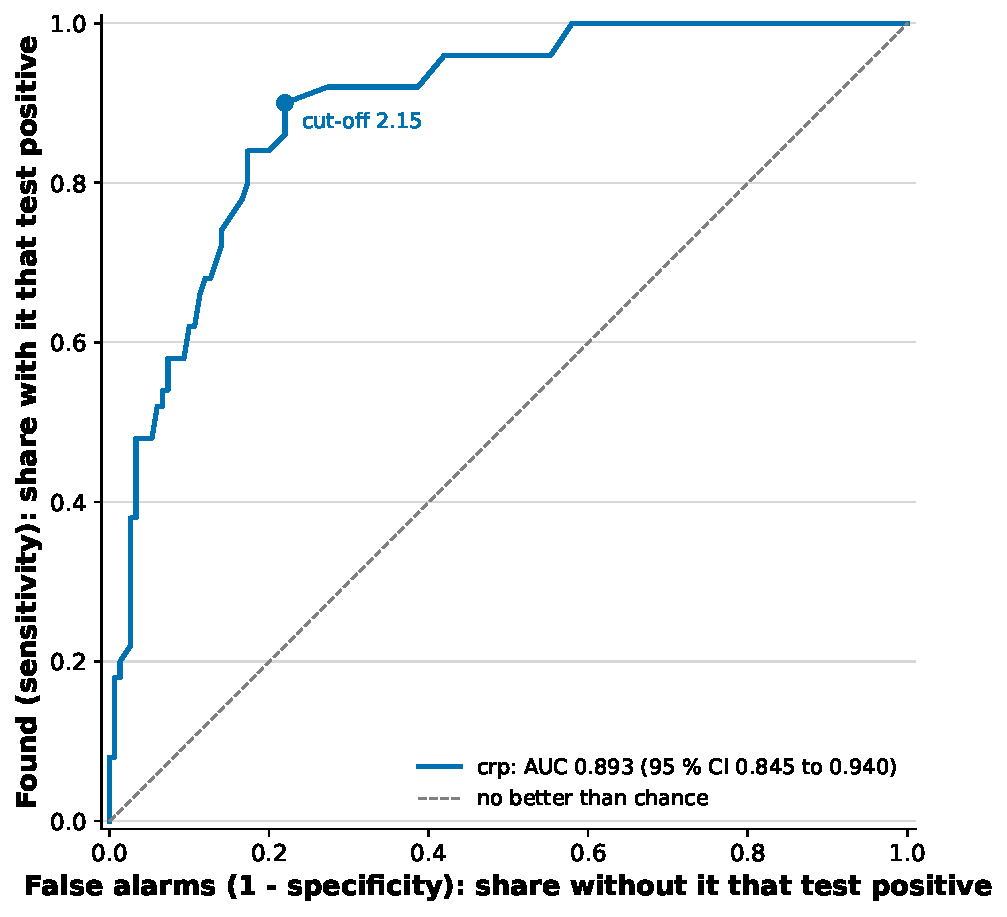
\includegraphics[width=0.52\textwidth,height=0.26\textheight,keepaspectratio]{figures/underneath_trade_off_curve.pdf}
\captionof*{figure}{The chart simplydata draws. The code below draws the same lines, without simplydata's paper look.}
\end{minipage}\end{center}
\needspace{10\baselineskip}\begin{underneathbox}{\libbadge{R}\libbadge{matplotlib}}
\underlib{R (simplydata runs this in R for you, through rpy2)}
\begin{lstlisting}[style=underr]
# trade_off_curve(score="crp", truth="infected")
# infected (1 = yes, 0 = no) and crp: two columns of sdata.get_example("clinic")
r <- pROC::roc(infected, crp, levels = c(0, 1),
               direction = "<", quiet = TRUE)      # (1)
ci <- pROC::ci.auc(r, method = "delong")           # (2)
p <- pROC::coords(r, "all", ret = c("specificity", "sensitivity"),
                  transpose = FALSE)
b <- pROC::coords(r, "best", best.method = "youden",
                  ret = c("specificity", "sensitivity"), transpose = FALSE)
list(x = 1 - p$specificity, y = p$sensitivity,
     best_x = 1 - b$specificity[1], best_y = b$sensitivity[1],
     auc = ci[2], auc_low = ci[1], auc_high = ci[3])
\end{lstlisting}
\underlib{matplotlib (with what R gives back)}
\begin{lstlisting}[style=under]
import matplotlib.pyplot as plt
import numpy as np
fig, ax = plt.subplots()
order = np.lexsort((y, x))
ax.plot(x[order], y[order])                         # the curve
ax.plot([best_x], [best_y], marker="o")             # (3)
ax.plot([0, 1], [0, 1], linestyle="--")             # no better than chance
\end{lstlisting}
\undertext{\textbf{simplydata chooses}}
\undertext{(1) higher scores count as positive (direction = \code{\textquotedbl{}\textless{}\textquotedbl{}}); \code{positive\_\allowbreak{}when=\textquotedbl{}lower\textquotedbl{}} turns it round.}
\undertext{(2) the AUC and its 95 \% interval by DeLong's method, written in the legend.}
\undertext{(3) the best cut-off by Youden's index (the most found cases minus false alarms) is marked with a dot.}
\undertext{\textit{In Python only:} Python's stack (SciPy, statsmodels) has no ROC analysis with DeLong's interval, so the numbers come from R.}
\undertext{simplydata also writes the AUC and the cut-off on the chart and labels both axes in words. simplydata also gives the chart its paper look (fonts, colours, no top and right lines); that is left out here.}
\undertext{\textit{Checked:} a test runs both and compares the lines and the numbers in the legend (the chart's data, not its pixels).}
\end{underneathbox}
\unsection{Agreement and reliability}{group:Agreement-and-reliability}
\wordentry{table.agreement\_between()}{word:table.agreement-between}
How well do two or more raters (or devices) agree on the same rows?

\codeline{table.agreement\_between(\textquotedbl{}nurse\_rating\textquotedbl{}, \textquotedbl{}doctor\_rating\textquotedbl{})   (with sdata.get\_example(\textquotedbl{}clinic\textquotedbl{}))}\\
Each column holds one rater's answers for the same rows. The kind of column decides, and the sentence says which: categories, 2 columns: Cohen's kappa (statsmodels, as R irr::\code{kappa2()}), with the raw agreement beside it; \code{near\_\allowbreak{}misses=\textquotedbl{}linear\textquotedbl{}} or \code{\textquotedbl{}quadratic\textquotedbl{}} counts near misses as partly right (ordered categories: give \code{in\_\allowbreak{}order=[\textquotedbl{}mild\textquotedbl{},\allowbreak{} \textquotedbl{}moderate\textquotedbl{},\allowbreak{} \textquotedbl{}severe\textquotedbl{}]}); categories, 3 or more columns: Fleiss' kappa (statsmodels; its p-value from R irr); numbers: the intraclass correlation (ICC) from R irr::\code{icc()}: by default two-way, absolute agreement, one rater, the raters a sample of many possible raters (\code{raters=\textquotedbl{}these only\textquotedbl{}} or \code{\textquotedbl{}different per row\textquotedbl{}}, \code{checking\_\allowbreak{}for=\textquotedbl{}consistency\textquotedbl{}}, \code{of=\textquotedbl{}average of raters\textquotedbl{}} choose another form, and the form is always named). \code{method=\textquotedbl{}krippendorff\textquotedbl{}}: Krippendorff's alpha (R irr::\code{kripp.\allowbreak{}alpha()}); \code{method=\textquotedbl{}lin\textquotedbl{}}: Lin's concordance correlation for two columns of numbers (R DescTools::\code{CCC()}). Rows with an empty cell are skipped. Gives back a one-row table.

\wordfield{Options}{}\par\nopagebreak
\begin{optiontable}
\code{columns.\allowbreak{}.\allowbreak{}.\allowbreak{}} & as many as you like, separated by commas\\
\code{method=} & \\
\code{near\_\allowbreak{}misses=} & \\
\code{in\_\allowbreak{}order=} & \\
\code{interval=} & normally \code{95}\\
\code{raters=} & normally \code{\textquotedbl{}a sample\textquotedbl{}}\\
\code{checking\_\allowbreak{}for=} & normally \code{\textquotedbl{}agreement\textquotedbl{}}\\
\code{of=} & normally \code{\textquotedbl{}one rater\textquotedbl{}}\\
\end{optiontable}

\wordfield{Underneath}{statsmodels (\code{inter\_\allowbreak{}rater}.cohens\_kappa, \code{fleiss\_\allowbreak{}kappa}); R irr::kappam.fleiss for the p-value of Fleiss' kappa, irr::icc, irr::kripp.alpha and DescTools::CCC (simplydata[r])}
\wordfield{Example you can run}{}\par\nopagebreak
\begin{lstlisting}[style=py]
import simplydata as sdata
table = sdata.table(sdata.get_example("clinic"))
table.agreement_between("nurse_rating", "doctor_rating")
table.agreement_between("device_a", "device_b")
\end{lstlisting}
\wordentry{table.limits\_of\_agreement()}{word:table.limits-of-agreement}
How far apart are two ways of measuring the same thing (Bland-Altman limits of agreement)?

\codeline{table.limits\_of\_agreement(\textquotedbl{}device\_a\textquotedbl{}, \textquotedbl{}device\_b\textquotedbl{})   (with sdata.get\_example(\textquotedbl{}clinic\textquotedbl{}))}\\
Each row is one thing measured both ways. Prints how much the first reads higher or lower on average, and the limits within which 95 \% of the differences lie (average difference plus and minus 1.96 standard deviations), each with its interval (R BlandAltmanLeh::\code{bland.\allowbreak{}altman.\allowbreak{}stats()}, simplydata[r]), and Lin's concordance correlation (R DescTools::\code{CCC()}). Whether the limits are close enough is a question for the field, not for statistics. \code{chart.\allowbreak{}difference\_\allowbreak{}dots(first=.\allowbreak{}.\allowbreak{}.\allowbreak{},\allowbreak{} second=.\allowbreak{}.\allowbreak{}.\allowbreak{})} draws it. Gives back a one-row table.

\wordfield{Options}{}\par\nopagebreak
\begin{optiontable}
\code{first=} & \\
\code{second=} & \\
\code{interval=} & normally \code{95}\\
\end{optiontable}

\wordfield{Underneath}{R BlandAltmanLeh::bland.altman.stats and DescTools::CCC (simplydata[r])}
\wordfield{Example you can run}{}\par\nopagebreak
\begin{lstlisting}[style=py]
import simplydata as sdata
table = sdata.table(sdata.get_example("clinic"))
table.limits_of_agreement("device_a", "device_b")
\end{lstlisting}
\wordentry{table.reliability\_of()}{word:table.reliability-of}
Do the items of a questionnaire hang together (Cronbach's alpha)?

\codeline{table.reliability\_of([\textquotedbl{}item\_1\textquotedbl{}, \textquotedbl{}item\_2\textquotedbl{}, \textquotedbl{}item\_3\textquotedbl{}, \textquotedbl{}item\_4\textquotedbl{}, \textquotedbl{}item\_5\textquotedbl{}])   (with sdata.get\_example(\textquotedbl{}clinic\textquotedbl{}))}\\
Each column is one item (question), each row one person. Prints Cronbach's alpha with Feldt's interval and what alpha would be without each item (R psych::\code{alpha()} and psych::\code{alpha.\allowbreak{}ci()}, simplydata[r]). Alpha rises with the number of items and does not show that the items measure one thing. Gives back one row for alpha and one per item.

\wordfield{Options}{}\par\nopagebreak
\begin{optiontable}
\code{columns.\allowbreak{}.\allowbreak{}.\allowbreak{}} & as many as you like, separated by commas\\
\code{interval=} & normally \code{95}\\
\end{optiontable}

\wordfield{Underneath}{R psych::alpha and psych::alpha.ci (simplydata[r])}
\wordfield{Example you can run}{}\par\nopagebreak
\begin{lstlisting}[style=py]
import simplydata as sdata
table = sdata.table(sdata.get_example("clinic"))
table.reliability_of(["item_1", "item_2", "item_3", "item_4", "item_5"])
\end{lstlisting}
\wordentry{chart.difference\_dots()}{word:difference-dots}
Do two ways of measuring agree? The difference of each pair against its average (Bland-Altman).\\
\codeline{chart.difference\_dots(first=\textquotedbl{}device\_a\textquotedbl{}, second=\textquotedbl{}device\_b\textquotedbl{}) (with sdata.get\_example(\textquotedbl{}clinic\textquotedbl{}))}

One dot per row: along, the average of the two measurements; up, first minus second. The names are those of \code{table.\allowbreak{}limits\_\allowbreak{}of\_\allowbreak{}agreement(first,\allowbreak{} second)}. The solid line is the average difference (does one read higher?), the dashed lines the limits of agreement, within which 95 \% of the differences lie (average plus and minus 1.96 standard deviations), each with its 95 \% interval shaded. The dots and the average come from statsmodels \code{mean\_\allowbreak{}diff\_\allowbreak{}plot}, the limits and their intervals from R BlandAltmanLeh::\code{bland.\allowbreak{}altman.\allowbreak{}stats()} (simplydata[r]), the same as\\
\codeline{table.limits\_of\_agreement(...).}

\wordfield{Options}{}\par\nopagebreak
\begin{optiontable}
\code{first=} & \\
\code{second=} & \\
\code{transparency=} & \\
\end{optiontable}

\wordfield{Underneath}{statsmodels (graphics.agreement.mean\_diff\_plot) for the dots; R BlandAltmanLeh::bland.altman.stats for the limits and their intervals (simplydata[r])}
\wordfield{Example you can run}{}\par\nopagebreak
\begin{lstlisting}[style=py]
import simplydata as sdata
clinic = sdata.get_example("clinic")
chart = sdata.chart(clinic)
chart.difference_dots(first="device_a", second="device_b")
chart.save("difference_dots.png")
\end{lstlisting}
\unsection{Fitting}{group:Fitting}
\wordentry{table.fit\_line()}{word:table.fit-line}
Fit the straight line y = slope * x + intercept that best follows the points.

\codeline{table.fit\_line(x=\textquotedbl{}hours\textquotedbl{}, y=\textquotedbl{}marks\textquotedbl{})   (with sdata.get\_example(\textquotedbl{}marks\textquotedbl{}))}\\
Ordinary least squares (the same as R \code{lm(y \textasciitilde{} x)}). Prints how much y goes up for each 1 more of x, with its 95 \% confidence interval and p-value, and R squared: the share of the differences in y that the line explains. Rows with an empty cell in x or y are skipped. A link does not show that x causes y. Gives back a one-row table. The same line as \code{chart.\allowbreak{}fit\_\allowbreak{}line()}; its old name \code{fit\_\allowbreak{}straight\_\allowbreak{}line} still works. For a curve use \code{fit\_\allowbreak{}curve()}, for any formula \code{fit\_\allowbreak{}formula()}.

\wordfield{Options}{}\par\nopagebreak
\begin{optiontable}
\code{x=} & \\
\code{y=} & \\
\end{optiontable}

\wordfield{Underneath}{SciPy \code{linregress()}, \code{t.\allowbreak{}ppf()}}
\wordfield{Example you can run}{}\par\nopagebreak
\begin{lstlisting}[style=py]
import simplydata as sdata
table = sdata.table(sdata.get_example("marks"))
table.fit_line(x="hours", y="marks")
\end{lstlisting}
\needspace{10\baselineskip}\begin{underneathbox}{\libbadge{SciPy}}
\underlib{SciPy}
\begin{lstlisting}[style=under]
from scipy import stats
df = sdata.get_example("marks")
# fit_line(x="hours", y="marks")
fit = stats.linregress(df["hours"], df["marks"])
t = stats.t.ppf(0.975, len(df) - 2)                 # (1)
{"slope": fit.slope, "intercept": fit.intercept,
 "slope standard error": fit.stderr, "intercept standard error": fit.intercept_stderr,
 "slope 95 % CI low": fit.slope - t * fit.stderr,
 "R squared": fit.rvalue ** 2, "p-value": fit.pvalue}
\end{lstlisting}
\undertext{\textbf{simplydata chooses}}
\undertext{(1) the 95 \% interval of the slope uses the t distribution with n - 2 degrees of freedom, as R's \code{confint(lm(.\allowbreak{}.\allowbreak{}.\allowbreak{}))}.}
\undertext{Rows with an empty cell in x or y are left out first. simplydata also writes the result as a sentence and names the test.}
\undertext{\textit{Checked:} a test runs both and compares the numbers of the result table (on a pandas and on a Polars table).}
\end{underneathbox}
\wordentry{table.fit\_curve()}{word:table.fit-curve}
Fit a curve y = b0 + b1 * x + b2 * x**2 ... that best follows the points.

\codeline{table.fit\_curve(x=\textquotedbl{}hours\textquotedbl{}, y=\textquotedbl{}marks\textquotedbl{}, of\_degree=2)   (with sdata.get\_example(\textquotedbl{}marks\textquotedbl{}))}\\
\code{of\_\allowbreak{}degree=2} is a curve with one bend, \code{of\_\allowbreak{}degree=3} can bend twice, and so on (up to 10), the same curve as \code{chart.\allowbreak{}fit\_\allowbreak{}curve(of\_\allowbreak{}degree=)}. Least squares on the powers of x, as R \code{lm(y \textasciitilde{} poly(x,\allowbreak{} 2,\allowbreak{} raw = TRUE))}. Prints the curve and R squared; gives back one row per term (the intercept, x, x**2 ...) with its estimate, standard error, t, p-value and 95 \% confidence interval. \code{weights=\textquotedbl{}column\textquotedbl{}} counts some rows more (as R \code{lm(weights =)}); \code{for\_\allowbreak{}each\_\allowbreak{}group\_\allowbreak{}in=\textquotedbl{}column\textquotedbl{}} fits each group on its own. Rows with an empty cell are skipped.

\wordfield{Options}{}\par\nopagebreak
\begin{optiontable}
\code{x=} & \\
\code{y=} & \\
\code{of\_\allowbreak{}degree=} & normally \code{2}\\
\code{weights=} & \\
\code{for\_\allowbreak{}each\_\allowbreak{}group\_\allowbreak{}in=} & \\
\end{optiontable}

\wordfield{Underneath}{statsmodels (WLS by QR on the powers of x, as R \code{lm(y \textasciitilde{} poly(x,\allowbreak{} raw = TRUE))})}
\wordfield{Example you can run}{}\par\nopagebreak
\begin{lstlisting}[style=py]
import simplydata as sdata
table = sdata.table(sdata.get_example("marks"))
table.fit_curve(x="hours", y="marks", of_degree=2)
\end{lstlisting}
\wordentry{table.fit\_formula()}{word:table.fit-formula}
Find the values in a formula that make it follow the data best.

\codeline{table.fit\_formula(\textquotedbl{}population = a * exp(b * (year - 2000))\textquotedbl{})   (with sdata.get\_example(\textquotedbl{}growth\textquotedbl{}))}\\
Write the column to fit on the left of =. On the right, names that are columns are data; any other name (such as a, b or rate) is a value to find. Uses nonlinear least squares, as R \code{nls()} (Levenberg-Marquardt). Every value to find starts at 1; give better start values with \code{start=}\{\code{\textquotedbl{}a\textquotedbl{}}: 10, \code{\textquotedbl{}b\textquotedbl{}}: 0.03\} if the fit fails. \code{between=}\{\code{\textquotedbl{}b\textquotedbl{}}: [0, None]\} keeps a value between limits (None: no limit), as R \code{nls(algorithm = \textquotedbl{}port\textquotedbl{})}; \code{search=\textquotedbl{}whole range\textquotedbl{}} searches the whole range of \code{between=} before fitting (differential evolution, seed 1), for when start values are hard to guess. \code{weights=\textquotedbl{}column\textquotedbl{}} counts some rows more (as R \code{nls(weights =)}). \code{for\_\allowbreak{}each\_\allowbreak{}group\_\allowbreak{}in=\textquotedbl{}column\textquotedbl{}} fits each group on its own. \code{method=} lets an expert choose \code{\textquotedbl{}levenberg-marquardt\textquotedbl{}}, \code{\textquotedbl{}trust region\textquotedbl{}} or \code{\textquotedbl{}dogbox\textquotedbl{}}. Prints each value with its 95 \% confidence interval, the residual standard error and R squared (only a rough guide for a curve). Gives back one row (one per group) with each value, its standard error, t, p-value and 95 \% CI, the residual standard error, degrees of freedom, R squared, AIC, rows and whether the fit converged. Residuals: \code{add\_\allowbreak{}predicted\_\allowbreak{}column} with the same formula, then \code{add\_\allowbreak{}column(\textquotedbl{}y - predicted y\textquotedbl{})}. Rows with an empty cell are skipped.

\wordfield{Options}{}\par\nopagebreak
\begin{optiontable}
\code{formula=} & \\
\code{start=} & \\
\code{between=} & \\
\code{weights=} & \\
\code{for\_\allowbreak{}each\_\allowbreak{}group\_\allowbreak{}in=} & \\
\code{search=} & normally \code{\textquotedbl{}from start\textquotedbl{}}\\
\code{method=} & \\
\end{optiontable}

\wordfield{Underneath}{SciPy (optimize.curve\_fit; optimize.differential\_evolution for \code{search=\textquotedbl{}whole range\textquotedbl{}})}
\wordfield{Example you can run}{}\par\nopagebreak
\begin{lstlisting}[style=py]
import simplydata as sdata
table = sdata.table(sdata.get_example("growth"))
table.fit_formula("population = a * exp(b * (year - 2000))", for_each_group_in="country")
table.keep_rows_where("country", is_equal_to="Applia")
table.fit_formula("population = a * exp(b * (year - 2000))")
\end{lstlisting}
\unsection{Finding and solving}{group:Finding-and-solving}
\wordentry{sdata.find\_where\_smallest()}{word:sdata.find-where-smallest}
Find where a formula is smallest, and its value there.

\codeline{sdata.find\_where\_smallest(\textquotedbl{}x**2 - 4*x + 1\textquotedbl{}, between=[0, 5])}\enspace (the smallest value is -3, at x = 2)\\
The names in the formula (x, y, a, rate) are what to find. Give a range with \code{between=} ([0, 5] for one name; \{\code{\textquotedbl{}x\textquotedbl{}}: [0, 5], \code{\textquotedbl{}y\textquotedbl{}}: [0, None]\} for several, None = no limit) or starting guesses with \code{start=} (a number, or \{\code{\textquotedbl{}x\textquotedbl{}}: 1, \code{\textquotedbl{}y\textquotedbl{}}: 2\}). \code{rules=[\textquotedbl{}x + y \textless{}= 4\textquotedbl{},\allowbreak{} \textquotedbl{}x \textgreater{}= 0\textquotedbl{}]} adds rules the answer must keep (=, \textless{}= or \textgreater{}=); \code{whole\_\allowbreak{}numbers=True} asks for whole numbers (with a straight-line formula and rules). \code{search=\textquotedbl{}whole range\textquotedbl{}} looks everywhere in \code{between=} instead of near the start. \code{known=}\{\code{\textquotedbl{}a\textquotedbl{}}: 2.1\} (or a one-row result table from \code{table.\allowbreak{}fit\_\allowbreak{}formula}) fixes some names. The method is decided by what you give and printed (R \code{optimize()}, \code{optim()}, lpSolve::\code{lp()}; see the module notes); \code{method=} lets experts choose (\code{\textquotedbl{}nelder-mead\textquotedbl{}}, \code{\textquotedbl{}bfgs\textquotedbl{}}, \code{\textquotedbl{}l-bfgs-b\textquotedbl{}}, \code{\textquotedbl{}conjugate gradient\textquotedbl{}}, \code{\textquotedbl{}powell\textquotedbl{}}, \code{\textquotedbl{}trust region\textquotedbl{}}, \code{\textquotedbl{}slsqp\textquotedbl{}}, \code{\textquotedbl{}cobyla\textquotedbl{}}; with \code{search=\textquotedbl{}whole range\textquotedbl{}}: \code{\textquotedbl{}differential evolution\textquotedbl{}}, \code{\textquotedbl{}dual annealing\textquotedbl{}}, \code{\textquotedbl{}shgo\textquotedbl{}}, \code{\textquotedbl{}basin hopping\textquotedbl{}}, \code{\textquotedbl{}direct\textquotedbl{}}). Gives back a one-row table: the value of each name, the smallest value, the method, whether the search settled, and for linear programs the value of one more on the right of each rule (shadow price, R \code{lp(compute.\allowbreak{}sens = TRUE)}\$duals). \code{fast=True} gives the table on the fast engine (Polars).

\wordfield{Options}{}\par\nopagebreak
\begin{optiontable}
\code{formula=} & \\
\code{between=} & \\
\code{start=} & \\
\code{rules=} & \\
\code{whole\_\allowbreak{}numbers=} & normally \code{False}\\
\code{search=} & normally \code{\textquotedbl{}from start\textquotedbl{}}\\
\code{method=} & \\
\code{known=} & \\
\code{fast=} & normally \code{False}\\
\end{optiontable}

\wordfield{Underneath}{SciPy (optimize.minimize\_scalar, minimize, linprog and milp with HiGHS, \code{differential\_\allowbreak{}evolution} and other global searches)}
\wordfield{Example you can run}{}\par\nopagebreak
\begin{lstlisting}[style=py]
import simplydata as sdata
sdata.find_where_smallest("x**2 - 4*x + 1", between=[0, 5])
sdata.find_where_smallest("(x - 1)**2 + (y - 2)**2", start={"x": 0, "y": 0})
\end{lstlisting}
\wordentry{sdata.find\_where\_biggest()}{word:sdata.find-where-biggest}
Find where a formula is biggest, and its value there.

\codeline{sdata.find\_where\_biggest(\textquotedbl{}3*x + 2*y\textquotedbl{}, rules=[\textquotedbl{}x + y \textless{}= 4\textquotedbl{}, \textquotedbl{}x + 3*y \textless{}= 6\textquotedbl{}, \textquotedbl{}x \textgreater{}= 0\textquotedbl{}, \textquotedbl{}y \textgreater{}= 0\textquotedbl{}])}\enspace (12, at x = 4, y = 0)\\
The same options as \code{find\_\allowbreak{}smallest()}: \code{between=}, \code{start=}, \code{rules=}, \code{whole\_\allowbreak{}numbers=}, \code{search=\textquotedbl{}whole range\textquotedbl{}}, \code{method=}, \code{known=} (a dict, or a one-row result table from \code{table.\allowbreak{}fit\_\allowbreak{}formula}, so a fitted curve can be handed straight over). It works by finding the smallest value of minus the formula, and prints the biggest. Gives back a one-row table: each name, the biggest value, the method, whether it settled, and for linear programs the value of one more on the right of each rule (shadow price).

\wordfield{Options}{}\par\nopagebreak
\begin{optiontable}
\code{formula=} & \\
\code{between=} & \\
\code{start=} & \\
\code{rules=} & \\
\code{whole\_\allowbreak{}numbers=} & normally \code{False}\\
\code{search=} & normally \code{\textquotedbl{}from start\textquotedbl{}}\\
\code{method=} & \\
\code{known=} & \\
\code{fast=} & normally \code{False}\\
\end{optiontable}

\wordfield{Underneath}{SciPy (the same as \code{find\_\allowbreak{}smallest}, on minus the formula)}
\wordfield{Example you can run}{}\par\nopagebreak
\begin{lstlisting}[style=py]
import simplydata as sdata
sdata.find_where_biggest("x * (10 - x)", between=[0, 10])
sdata.find_where_biggest("3*x + 2*y", rules=["x + y <= 4", "x + 3*y <= 6", "x >= 0", "y >= 0"])
\end{lstlisting}
\wordentry{sdata.solve()}{word:sdata.solve}
Find the values that make an equation true.

\codeline{sdata.solve(\textquotedbl{}x**3 - 2*x = 5\textquotedbl{}, between=[0, 3])}\enspace (x = 2.09455)\\
One equation with one name: \code{between=[low,\allowbreak{} high]} finds every solution in the range where the two sides cross (Brent's method, R \code{uniroot()} on each sign change, as rootSolve::\code{uniroot.\allowbreak{}all()}); \code{start=} finds one solution by searching from the start (secant method); a polynomial (only + - * and whole powers) needs neither and gives all its solutions, complex ones too (R \code{polyroot()}). Several equations in a list:\\
\codeline{sdata.solve([\textquotedbl{}x + y = 3\textquotedbl{}, \textquotedbl{}x * y = 2\textquotedbl{}], start=\{\textquotedbl{}x\textquotedbl{}: 0, \textquotedbl{}y\textquotedbl{}: 1\}) (Powell's hybrid method, as}\\
R nleqslv::\code{nleqslv()}); straight-line equations are solved exactly (R \code{solve()}). \code{known=} fixes some names (a dict, or a one-row result table from \code{table.\allowbreak{}fit\_\allowbreak{}formula}). Gives back a table with one row per solution: each name, \code{\textquotedbl{}left minus right\textquotedbl{}} at the solution (the check: close to 0) and the method. \code{fast=True} gives a Polars table.

\wordfield{Options}{}\par\nopagebreak
\begin{optiontable}
\code{equations=} & \\
\code{between=} & \\
\code{start=} & \\
\code{method=} & \\
\code{known=} & \\
\code{fast=} & normally \code{False}\\
\end{optiontable}

\wordfield{Underneath}{SciPy (optimize.brentq, \code{root\_\allowbreak{}scalar}, root) and NumPy (polynomial roots, linalg.solve)}
\wordfield{Example you can run}{}\par\nopagebreak
\begin{lstlisting}[style=py]
import simplydata as sdata
sdata.solve("x**3 - 2*x = 5", between=[0, 3])
sdata.solve("x**2 - 2*x + 5 = 0")
sdata.solve(["x + y = 3", "x * y = 2"], start={"x": 0, "y": 1})
\end{lstlisting}
\unsection{Values between points}{group:Values-between-points}
\wordentry{table.values\_at()}{word:table.values-at}
Estimate a column at places between the known points, by joining the dots.

\codeline{table.values\_at(\textquotedbl{}population\textquotedbl{}, at=\{\textquotedbl{}year\textquotedbl{}: [2001, 2003, 2011]\}, for\_each\_group\_in=\textquotedbl{}country\textquotedbl{})   (with sdata.get\_example(\textquotedbl{}growth\textquotedbl{}))}\\
\code{at=} names the \code{column(s)} that place the points and the places wanted. One column joins the points along a line; two or more (\code{at=}\{\code{\textquotedbl{}east\textquotedbl{}}: [1.5, 2.5], \code{\textquotedbl{}north\textquotedbl{}}: [3, 4.5]\},\\
\codeline{sdata.get\_example(\textquotedbl{}island\textquotedbl{})) join them across a surface: the lists are read as pairs,}\\
(1.5, 3) and (2.5, 4.5); \code{table.\allowbreak{}make\_\allowbreak{}map\_\allowbreak{}of()} gives every combination. \code{joined\_\allowbreak{}by=} says how the points are joined (one column): \code{\textquotedbl{}straight lines\textquotedbl{}} (default, linear interpolation, R \code{approx()}), \code{\textquotedbl{}smooth curve\textquotedbl{}} (natural cubic spline, R \code{splinefun(method = \textquotedbl{}natural\textquotedbl{})}), \code{\textquotedbl{}curve without overshoot\textquotedbl{}} (PCHIP), \code{\textquotedbl{}steps\textquotedbl{}}, \code{\textquotedbl{}nearest\textquotedbl{}}; experts: \code{\textquotedbl{}akima\textquotedbl{}}, \code{\textquotedbl{}makima\textquotedbl{}}, \code{\textquotedbl{}not-a-knot\textquotedbl{}}, \code{\textquotedbl{}periodic\textquotedbl{}}. Two or more columns: \code{\textquotedbl{}straight lines\textquotedbl{}} (bilinear on a full grid, triangles otherwise), \code{\textquotedbl{}smooth surface\textquotedbl{}} (thin-plate spline), \code{\textquotedbl{}nearest\textquotedbl{}}; on a full grid also \code{\textquotedbl{}cubic\textquotedbl{}}, \code{\textquotedbl{}quintic\textquotedbl{}}, \code{\textquotedbl{}pchip\textquotedbl{}}. \code{smoothness=\textquotedbl{}auto\textquotedbl{}} or a number gives a smoothing spline that passes near, not through, the points (R \code{smooth.\allowbreak{}spline()}; a number is R's \code{lambda=}); 0 passes through every point. \code{\textquotedbl{}auto\textquotedbl{}} lets R itself choose the smoothness and needs R (pip install \code{\textquotedbl{}simplydata[r]\textquotedbl{}}); a number needs no R. \code{outside=} is what happens beyond the known points: \code{\textquotedbl{}empty\textquotedbl{}} (default), \code{\textquotedbl{}nearest end\textquotedbl{}} or \code{\textquotedbl{}extend\textquotedbl{}} (curves only; guesswork). \code{for\_\allowbreak{}each\_\allowbreak{}group\_\allowbreak{}in=\textquotedbl{}country\textquotedbl{}} joins each group on its own. Rows with an empty cell are skipped. Gives back a new table: the \code{at=} columns, the \code{for\_\allowbreak{}each\_\allowbreak{}group\_\allowbreak{}in=} columns and the estimated column.

\wordfield{Options}{}\par\nopagebreak
\begin{optiontable}
\code{column=} & \\
\code{at=} & \\
\code{joined\_\allowbreak{}by=} & normally \code{\textquotedbl{}straight lines\textquotedbl{}}\\
\code{smoothness=} & normally \code{0}\\
\code{for\_\allowbreak{}each\_\allowbreak{}group\_\allowbreak{}in=} & \\
\code{outside=} & normally \code{\textquotedbl{}empty\textquotedbl{}}\\
\end{optiontable}

\wordfield{Underneath}{NumPy (interp) and SciPy (interpolate: CubicSpline, PchipInterpolator, Akima1DInterpolator, \code{make\_\allowbreak{}smoothing\_\allowbreak{}spline}, griddata, RegularGridInterpolator, RBFInterpolator); \code{smoothness=\textquotedbl{}auto\textquotedbl{}} lets R smooth.spline choose the smoothness (needs R)}
\wordfield{Example you can run}{}\par\nopagebreak
\begin{lstlisting}[style=py]
import simplydata as sdata
table = sdata.table(sdata.get_example("growth"))
estimates = table.values_at("population", at={"year": [2001, 2003, 2011]}, for_each_group_in="country")
estimates.show()
table.values_at("population", at={"year": [2001, 2003, 2011]}, joined_by="smooth curve", for_each_group_in="country")
\end{lstlisting}
\wordentry{table.make\_map\_of()}{word:table.make-map-of}
Estimate a column at evenly spaced places across one or more columns (a map), ready for a contour or heatmap.

\codeline{table.make\_map\_of(\textquotedbl{}height\textquotedbl{}, across=[\textquotedbl{}east\textquotedbl{}, \textquotedbl{}north\textquotedbl{}], steps=100)   (with sdata.get\_example(\textquotedbl{}island\textquotedbl{}))}\\
The map runs from the smallest to the biggest known value of each \code{across=} column, with \code{steps=} places along each (a number, or one per column). The points are joined as in \code{table.\allowbreak{}values\_\allowbreak{}at()} (same \code{joined\_\allowbreak{}by=} and \code{smoothness=}; \code{smoothness=\textquotedbl{}auto\textquotedbl{}} needs R, a number does not). Places outside the outline of the known points stay empty, with a note. Gives back a new long table: one row per place, with the \code{across=} columns and the estimated column.

\wordfield{Options}{}\par\nopagebreak
\begin{optiontable}
\code{column=} & \\
\code{across=} & \\
\code{steps=} & normally \code{50}\\
\code{joined\_\allowbreak{}by=} & normally \code{\textquotedbl{}straight lines\textquotedbl{}}\\
\code{smoothness=} & normally \code{0}\\
\end{optiontable}

\wordfield{Underneath}{SciPy (interpolate: RegularGridInterpolator, griddata, RBFInterpolator)}
\wordfield{Example you can run}{}\par\nopagebreak
\begin{lstlisting}[style=py]
import simplydata as sdata
table = sdata.table(sdata.get_example("island"))
heights = table.make_map_of("height", across=["east", "north"], steps=60, joined_by="smooth surface")
chart = heights.start_chart()
chart.draw_contour(x="east", y="north", z="height")
chart.save("map_of.png")
\end{lstlisting}
\unsection{Distributions}{group:Distributions}
\wordentry{sdata.distribution()}{word:sdata.distribution}
Make a distribution to ask chances, percentiles and random numbers of.

\codeline{dist = sdata.distribution(\textquotedbl{}normal\textquotedbl{}, average=50, standard\_deviation=10)}\\
then \code{dist.\allowbreak{}find\_\allowbreak{}chance\_\allowbreak{}that\_\allowbreak{}value(is\_\allowbreak{}above=80)}, \code{dist.\allowbreak{}find\_\allowbreak{}percentile(95)}, \code{dist.\allowbreak{}make\_\allowbreak{}random\_\allowbreak{}numbers(how\_\allowbreak{}many=100,\allowbreak{} with\_\allowbreak{}seed=1)}. Names: normal, lognormal, exponential, gamma, beta, uniform, t, chi-square, F, weibull, cauchy, logistic, laplace, gumbel, pareto, triangular, half-normal, inverse gaussian, von mises; for counts binomial, bernoulli, poisson, negative binomial, geometric, hypergeometric, whole number uniform. Parameters are R's with plain names; R's names (\code{mean=}, \code{sd=}, \code{prob=}, \code{size=}, \code{df=}, ...) work too. Any other SciPy distribution by its SciPy name and SciPy's parameters: \code{sdata.\allowbreak{}distribution(\textquotedbl{}burr12\textquotedbl{},\allowbreak{} c=2,\allowbreak{} d=3)}.

\wordfield{Options}{}\par\nopagebreak
\begin{optiontable}
\code{name=} & \\
\code{values.\allowbreak{}.\allowbreak{}.\allowbreak{}} & as many as you like, separated by commas\\
\end{optiontable}

\wordfield{Underneath}{SciPy (scipy.stats frozen distributions)}
\wordfield{Example you can run}{}\par\nopagebreak
\begin{lstlisting}[style=py]
import simplydata as sdata
dist = sdata.distribution("normal", average=50, standard_deviation=10)
print(dist)
dist.find_chance_that_value(is_above=80)
coins = sdata.distribution("binomial", tries=10, chance=0.5)
coins.find_chance_that_value(is_at_most=3)
\end{lstlisting}
\wordentry{table.fit\_distribution\_to()}{word:table.fit-distribution-to}
Fit a distribution to a column by maximum likelihood; gives back the fitted distribution.

\codeline{fit = table.fit\_distribution\_to(\textquotedbl{}sales\textquotedbl{}, \textquotedbl{}lognormal\textquotedbl{})   (with sdata.get\_example(\textquotedbl{}shop\textquotedbl{}))}\\
then \code{fit.\allowbreak{}find\_\allowbreak{}chance\_\allowbreak{}that\_\allowbreak{}value(is\_\allowbreak{}above=600)}, \code{fit.\allowbreak{}find\_\allowbreak{}percentile(90)}, \code{fit.\allowbreak{}draw\_\allowbreak{}chart()}, and \code{fit.\allowbreak{}turn\_\allowbreak{}into\_\allowbreak{}table()} for the result table (values, standard errors, log-likelihood, AIC, BIC, rows). As R MASS::\code{fitdistr(x,\allowbreak{} \textquotedbl{}gamma\textquotedbl{})} (fitdistrplus::fitdist for beta and others); standard errors from the observed information. Families without a location in R (gamma, weibull, lognormal, exponential, beta) keep it at 0, as R. \code{fixed=}\{\code{\textquotedbl{}shape\textquotedbl{}}: 2\} holds a parameter. With \code{for\_\allowbreak{}each\_\allowbreak{}group\_\allowbreak{}in=} it gives back a result table, one row per group. Empty cells are skipped. \code{\textquotedbl{}kernel density\textquotedbl{}} gives a smooth curve that follows the values, with no family chosen: SciPy \code{gaussian\_\allowbreak{}kde} with Silverman's bandwidth (statsmodels \code{bw\_\allowbreak{}silverman}), as R \code{density(x)}.

\wordfield{Options}{}\par\nopagebreak
\begin{optiontable}
\code{column=} & \\
\code{distribution=} & normally \code{\textquotedbl{}normal\textquotedbl{}}\\
\code{for\_\allowbreak{}each\_\allowbreak{}group\_\allowbreak{}in=} & \\
\code{fixed=} & \\
\end{optiontable}

\wordfield{Underneath}{SciPy (scipy.stats .fit and optimize, maximum likelihood; closed forms where they exist) and statsmodels (numdiff.approx\_hess3, for the standard errors); for \code{\textquotedbl{}kernel density\textquotedbl{}} SciPy \code{gaussian\_\allowbreak{}kde} with statsmodels \code{bw\_\allowbreak{}silverman}}
\wordfield{Example you can run}{}\par\nopagebreak
\begin{lstlisting}[style=py]
import simplydata as sdata
table = sdata.table(sdata.get_example("shop"))
fit = table.fit_distribution_to("sales", "lognormal")
fit.find_chance_that_value(is_above=600)
fit.turn_into_table()
\end{lstlisting}
\wordentry{table.compare\_distributions\_for()}{word:table.compare-distributions-for}
Fit several distributions to a column and rank them by AIC (smaller is better).

\codeline{table.compare\_distributions\_for(\textquotedbl{}sales\textquotedbl{})   (with sdata.get\_example(\textquotedbl{}shop\textquotedbl{}))}\\
\code{distributions=}(\code{\textquotedbl{}normal\textquotedbl{}}, \code{\textquotedbl{}lognormal\textquotedbl{}}, \code{\textquotedbl{}gamma\textquotedbl{}}, \code{\textquotedbl{}weibull\textquotedbl{}}) by default. Each is fitted by maximum likelihood (as \code{fit\_\allowbreak{}distribution\_\allowbreak{}to}); the result table has one row per distribution with its values, log-likelihood, AIC, BIC, the AIC difference from the best, and the Anderson-Darling, Kolmogorov-Smirnov and Cramer-von Mises statistics, as R fitdistrplus::\code{gofstat()}. An AIC difference below 2 is too small to choose between them.

\wordfield{Options}{}\par\nopagebreak
\begin{optiontable}
\code{column=} & \\
\code{distributions=} & normally \code{('normal',\allowbreak{} 'lognormal',\allowbreak{} 'gamma',\allowbreak{} 'weibull')}\\
\code{for\_\allowbreak{}each\_\allowbreak{}group\_\allowbreak{}in=} & \\
\end{optiontable}

\wordfield{Underneath}{SciPy (scipy.stats, maximum likelihood; Anderson-Darling, Kolmogorov-Smirnov and Cramer-von Mises statistics)}
\wordfield{Example you can run}{}\par\nopagebreak
\begin{lstlisting}[style=py]
import simplydata as sdata
table = sdata.table(sdata.get_example("shop"))
table.compare_distributions_for("sales")
\end{lstlisting}
\wordentry{nums.fit\_distribution()}{word:nums.fit-distribution}
Fit a distribution to the numbers by maximum likelihood; gives back the fitted distribution.

\codeline{fit = nums.fit\_distribution(\textquotedbl{}gamma\textquotedbl{})}\enspace then \code{fit.\allowbreak{}find\_\allowbreak{}chance\_\allowbreak{}that\_\allowbreak{}value(is\_\allowbreak{}above=10)}, \code{fit.\allowbreak{}turn\_\allowbreak{}into\_\allowbreak{}table()}\\
As R MASS::\code{fitdistr(x,\allowbreak{} \textquotedbl{}gamma\textquotedbl{})}; see \code{table.\allowbreak{}fit\_\allowbreak{}distribution\_\allowbreak{}to}. Empty values are skipped.

\wordfield{Options}{}\par\nopagebreak
\begin{optiontable}
\code{distribution=} & normally \code{\textquotedbl{}normal\textquotedbl{}}\\
\code{fixed=} & \\
\end{optiontable}

\wordfield{Underneath}{SciPy (scipy.stats and optimize, as \code{table.\allowbreak{}fit\_\allowbreak{}distribution\_\allowbreak{}to})}
\wordfield{Example you can run}{}\par\nopagebreak
\begin{lstlisting}[style=py]
import simplydata as sdata
nums = sdata.numbers([12, 15, 9, 20, 14])
fit = nums.fit_distribution("gamma")
fit.find_chance_that_value(is_above=18)
\end{lstlisting}
\wordentry{dist.find\_chance\_that\_value()}{word:dist.find-chance-that-value}
The chance of a value in a range, as a share from 0 to 1 (printed as a percent).

\codeline{dist.find\_chance\_that\_value(is\_above=80)}\enspace \code{dist.\allowbreak{}find\_\allowbreak{}chance\_\allowbreak{}that\_\allowbreak{}value(is\_\allowbreak{}below=60)} \code{dist.\allowbreak{}find\_\allowbreak{}chance\_\allowbreak{}that\_\allowbreak{}value(is\_\allowbreak{}between=[40,\allowbreak{} 60])}\\
\code{is\_\allowbreak{}at\_\allowbreak{}most=} and \code{is\_\allowbreak{}at\_\allowbreak{}least=} include the number itself; \code{is\_\allowbreak{}above=} and \code{is\_\allowbreak{}below=} do not (as \code{keep\_\allowbreak{}rows\_\allowbreak{}where}). For counts, \code{dist.\allowbreak{}find\_\allowbreak{}chance\_\allowbreak{}that\_\allowbreak{}value(3)} is the chance of exactly 3; \code{is\_\allowbreak{}below=3} means 0, 1 or 2 and \code{is\_\allowbreak{}at\_\allowbreak{}most=3} means 3 or fewer (R \code{pbinom(3)}). One lower option (\code{is\_\allowbreak{}above=}, \code{is\_\allowbreak{}at\_\allowbreak{}least=}) and one upper option (\code{is\_\allowbreak{}below=}, \code{is\_\allowbreak{}at\_\allowbreak{}most=}) can go together. A list gives Numbers. R: \code{pnorm(q,\allowbreak{} lower.\allowbreak{}tail = )}, dbinom.

\wordfield{Options}{}\par\nopagebreak
\begin{optiontable}
\code{value=} & \\
\code{is\_\allowbreak{}above=} & \\
\code{is\_\allowbreak{}below=} & \\
\code{is\_\allowbreak{}at\_\allowbreak{}most=} & \\
\code{is\_\allowbreak{}at\_\allowbreak{}least=} & \\
\code{is\_\allowbreak{}between=} & \\
\end{optiontable}

\wordfield{Underneath}{SciPy \code{norm()}, \code{sf()}}
\wordfield{Example you can run}{}\par\nopagebreak
\begin{lstlisting}[style=py]
import simplydata as sdata
dist = sdata.distribution("normal", average=50, standard_deviation=10)
dist.find_chance_that_value(is_above=80)
dist.find_chance_that_value(is_between=[40, 60])
dice = sdata.distribution("whole number uniform", between=[1, 6])
dice.find_chance_that_value(6)
\end{lstlisting}
\needspace{10\baselineskip}\begin{underneathbox}{\libbadge{SciPy}}
\underlib{SciPy}
\begin{lstlisting}[style=under]
from scipy import stats
dist = stats.norm(loc=50, scale=10)
# find_chance_that_value(is_above=80)
dist.sf(80)                     # (1)
\end{lstlisting}
\undertext{\textbf{simplydata chooses}}
\undertext{(1) the chance above a value is the survival function \code{sf()}, not 1 - \code{cdf()}: it stays accurate far out in the tail.}
\undertext{simplydata also says the chance in a sentence, with the same call in R (\code{pnorm(80,\allowbreak{} mean = 50,\allowbreak{} sd = 10,\allowbreak{} lower.\allowbreak{}tail = FALSE)}).}
\undertext{\textit{Checked:} a test runs both and compares the number.}
\end{underneathbox}
\wordentry{dist.find\_density\_at()}{word:dist.find-density-at}
The height of the density curve at a value (continuous distributions).

\codeline{dist.find\_density\_at(60)}\enspace (R \code{dnorm(60,\allowbreak{} mean = 50,\allowbreak{} sd = 10)}). A list gives Numbers.\\
It is not a chance: a chance is an area under the curve (\code{dist.\allowbreak{}find\_\allowbreak{}chance\_\allowbreak{}that\_\allowbreak{}value(is\_\allowbreak{}between=[.\allowbreak{}.\allowbreak{}.\allowbreak{}])}).

\wordfield{Options}{}\par\nopagebreak
\begin{optiontable}
\code{value=} & \\
\end{optiontable}

\wordfield{Underneath}{SciPy (scipy.stats frozen distributions: cdf, sf, ppf, isf, pdf, pmf, stats, rvs)}
\wordfield{Example you can run}{}\par\nopagebreak
\begin{lstlisting}[style=py]
import simplydata as sdata
dist = sdata.distribution("normal", average=50, standard_deviation=10)
dist.find_density_at(60)
\end{lstlisting}
\wordentry{dist.find\_percentile()}{word:dist.find-percentile}
The value that this percent of the distribution is below: \code{find\_\allowbreak{}percentile(95)}.

\codeline{dist.find\_percentile(95)}\enspace (R \code{qnorm(0.\allowbreak{}95,\allowbreak{} mean = 50,\allowbreak{} sd = 10)}). \code{find\_\allowbreak{}percentile(50)} is the median.\\
For counts: the smallest count with at least that percent at or below it (R qbinom). A list of percents gives Numbers.

\wordfield{Options}{}\par\nopagebreak
\begin{optiontable}
\code{percent=} & \\
\end{optiontable}

\wordfield{Underneath}{SciPy (scipy.stats frozen distributions: cdf, sf, ppf, isf, pdf, pmf, stats, rvs)}
\wordfield{Example you can run}{}\par\nopagebreak
\begin{lstlisting}[style=py]
import simplydata as sdata
dist = sdata.distribution("normal", average=50, standard_deviation=10)
dist.find_percentile(95)
dist.find_percentile([5, 50, 95])
\end{lstlisting}
\wordentry{dist.find\_cut\_off()}{word:dist.find-cut-off}
The value with this chance above it (or below it): critical values.

\codeline{dist.find\_cut\_off(with\_chance\_above=0.025)}\enspace the value with a 2.5 \% chance above it (R \code{qnorm(0.\allowbreak{}025,\allowbreak{} lower.\allowbreak{}tail = FALSE)})\\
\codeline{dist.find\_cut\_off(with\_chance\_below=0.05)}\enspace the value with a 5 \% chance below it\\
Chances are shares from 0 to 1. A list gives Numbers.

\wordfield{Options}{}\par\nopagebreak
\begin{optiontable}
\code{with\_\allowbreak{}chance\_\allowbreak{}above=} & \\
\code{with\_\allowbreak{}chance\_\allowbreak{}below=} & \\
\end{optiontable}

\wordfield{Underneath}{SciPy (scipy.stats frozen distributions: cdf, sf, ppf, isf, pdf, pmf, stats, rvs)}
\wordfield{Example you can run}{}\par\nopagebreak
\begin{lstlisting}[style=py]
import simplydata as sdata
dist = sdata.distribution("normal", average=50, standard_deviation=10)
dist.find_cut_off(with_chance_above=0.025)
dist.find_cut_off(with_chance_below=0.05)
\end{lstlisting}
\wordentry{dist.find\_middle\_range()}{word:dist.find-middle-range}
The range that holds the middle percent of the distribution, as Numbers [low, high].

\codeline{dist.find\_middle\_range(95)}\enspace (R \code{qnorm(c(0.\allowbreak{}025,\allowbreak{} 0.\allowbreak{}975),\allowbreak{} mean = 50,\allowbreak{} sd = 10)})

\wordfield{Options}{}\par\nopagebreak
\begin{optiontable}
\code{percent=} & normally \code{95}\\
\end{optiontable}

\wordfield{Underneath}{SciPy (scipy.stats frozen distributions: cdf, sf, ppf, isf, pdf, pmf, stats, rvs)}
\wordfield{Example you can run}{}\par\nopagebreak
\begin{lstlisting}[style=py]
import simplydata as sdata
dist = sdata.distribution("normal", average=50, standard_deviation=10)
dist.find_middle_range(95)
\end{lstlisting}
\wordentry{dist.find\_average()}{word:dist.find-average}
The average (mean) of the distribution. \code{dist.\allowbreak{}find\_\allowbreak{}average()}

\wordfield{Options}{none: just write the empty brackets.}

\wordfield{Underneath}{SciPy (scipy.stats frozen distributions: cdf, sf, ppf, isf, pdf, pmf, stats, rvs)}
\wordfield{Example you can run}{}\par\nopagebreak
\begin{lstlisting}[style=py]
import simplydata as sdata
dist = sdata.distribution("normal", average=50, standard_deviation=10)
dist.find_average()
\end{lstlisting}
\wordentry{dist.find\_median()}{word:dist.find-median}
The median: half of the distribution is below it. \code{dist.\allowbreak{}find\_\allowbreak{}median()}

\wordfield{Options}{none: just write the empty brackets.}

\wordfield{Underneath}{SciPy (scipy.stats frozen distributions: cdf, sf, ppf, isf, pdf, pmf, stats, rvs)}
\wordfield{Example you can run}{}\par\nopagebreak
\begin{lstlisting}[style=py]
import simplydata as sdata
dist = sdata.distribution("normal", average=50, standard_deviation=10)
dist.find_median()
\end{lstlisting}
\wordentry{dist.find\_standard\_deviation()}{word:dist.find-standard-deviation}
The standard deviation of the distribution. \code{dist.\allowbreak{}find\_\allowbreak{}standard\_\allowbreak{}deviation()}

\wordfield{Options}{none: just write the empty brackets.}

\wordfield{Underneath}{SciPy (scipy.stats frozen distributions: cdf, sf, ppf, isf, pdf, pmf, stats, rvs)}
\wordfield{Example you can run}{}\par\nopagebreak
\begin{lstlisting}[style=py]
import simplydata as sdata
dist = sdata.distribution("normal", average=50, standard_deviation=10)
dist.find_standard_deviation()
\end{lstlisting}
\wordentry{dist.find\_variance()}{word:dist.find-variance}
The variance (the standard deviation squared). \code{dist.\allowbreak{}find\_\allowbreak{}variance()}

\wordfield{Options}{none: just write the empty brackets.}

\wordfield{Underneath}{SciPy (scipy.stats frozen distributions: cdf, sf, ppf, isf, pdf, pmf, stats, rvs)}
\wordfield{Example you can run}{}\par\nopagebreak
\begin{lstlisting}[style=py]
import simplydata as sdata
dist = sdata.distribution("normal", average=50, standard_deviation=10)
dist.find_variance()
\end{lstlisting}
\wordentry{dist.show\_summary()}{word:dist.show-summary}
A one-row table: average, median, standard deviation, variance, skewness, excess kurtosis, entropy and the lowest and highest possible values. \code{dist.\allowbreak{}show\_\allowbreak{}summary()}

\wordfield{Options}{none: just write the empty brackets.}

\wordfield{Underneath}{SciPy (scipy.stats frozen distributions: cdf, sf, ppf, isf, pdf, pmf, stats, rvs)}
\wordfield{Example you can run}{}\par\nopagebreak
\begin{lstlisting}[style=py]
import simplydata as sdata
dist = sdata.distribution("normal", average=50, standard_deviation=10)
dist.show_summary()
\end{lstlisting}
\wordentry{dist.make\_random\_numbers()}{word:dist.make-random-numbers}
Numbers drawn at random from the distribution; the same seed gives the same numbers.

\codeline{dist.make\_random\_numbers(how\_many=100, with\_seed=1)}\enspace (\code{rows=} and \code{columns=} give a grid)\\
R's \code{rnorm()} and friends use another random number generator, so their numbers differ.

\wordfield{Options}{}\par\nopagebreak
\begin{optiontable}
\code{how\_\allowbreak{}many=} & \\
\code{with\_\allowbreak{}seed=} & normally \code{1}\\
\code{rows=} & \\
\code{columns=} & \\
\end{optiontable}

\wordfield{Underneath}{SciPy (scipy.stats frozen distributions: cdf, sf, ppf, isf, pdf, pmf, stats, rvs)}
\wordfield{Example you can run}{}\par\nopagebreak
\begin{lstlisting}[style=py]
import simplydata as sdata
dist = sdata.distribution("normal", average=50, standard_deviation=10)
nums = dist.make_random_numbers(how_many=100, with_seed=1)
nums.find_average()
\end{lstlisting}
\wordentry{dist.draw\_chart()}{word:dist.draw-chart}
A chart of the distribution: its density curve (or bars for counts).

\codeline{dist.draw\_chart()}\enspace or \code{dist.\allowbreak{}draw\_\allowbreak{}chart(show=\textquotedbl{}cumulative\textquotedbl{})} for the chance of a value at or below x.

\wordfield{Options}{}\par\nopagebreak
\begin{optiontable}
\code{show=} & normally \code{\textquotedbl{}density\textquotedbl{}}\\
\code{between=} & \\
\end{optiontable}

\wordfield{Underneath}{SciPy (scipy.stats frozen distributions: cdf, sf, ppf, isf, pdf, pmf, stats, rvs)}
\wordfield{Example you can run}{}\par\nopagebreak
\begin{lstlisting}[style=py]
import simplydata as sdata
dist = sdata.distribution("normal", average=50, standard_deviation=10)
chart = dist.draw_chart()
chart.write_title_on_top("Normal, average 50, standard deviation 10")
chart.save("distribution.png")
\end{lstlisting}
\wordentry{dist.turn\_into\_table()}{word:dist.turn-into-table}
A one-row table: the distribution, its parameters and, for a fit, the standard errors, log-likelihood, AIC and BIC. \code{dist.\allowbreak{}turn\_\allowbreak{}into\_\allowbreak{}table()}

\wordfield{Options}{none: just write the empty brackets.}

\wordfield{Underneath}{SciPy (scipy.stats frozen distributions: cdf, sf, ppf, isf, pdf, pmf, stats, rvs)}
\wordfield{Example you can run}{}\par\nopagebreak
\begin{lstlisting}[style=py]
import simplydata as sdata
dist = sdata.distribution("normal", average=50, standard_deviation=10)
result = dist.turn_into_table()
result.show()
\end{lstlisting}
\wordentry{dist.show\_parameters()}{word:dist.show-parameters}
The parameters as a dictionary of plain names: \{\code{\textquotedbl{}average\textquotedbl{}}: 50, \code{\textquotedbl{}standard\_\allowbreak{}deviation\textquotedbl{}}: 10\}. \code{dist.\allowbreak{}show\_\allowbreak{}parameters()}

\wordfield{Options}{none: just write the empty brackets.}

\wordfield{Underneath}{SciPy (scipy.stats frozen distributions: cdf, sf, ppf, isf, pdf, pmf, stats, rvs)}
\wordfield{Example you can run}{}\par\nopagebreak
\begin{lstlisting}[style=py]
import simplydata as sdata
dist = sdata.distribution("normal", average=50, standard_deviation=10)
print(dist.show_parameters())
\end{lstlisting}
\unsection{Models}{group:Models}
\wordentry{table.explain()}{word:table.explain}
Explain one column from several others with a model, and say how big each effect is.

\codeline{table.explain(\textquotedbl{}marks\textquotedbl{}, using=[\textquotedbl{}hours\textquotedbl{}, \textquotedbl{}breakfast\textquotedbl{}])   (with sdata.get\_example(\textquotedbl{}school\textquotedbl{}))}\\
\code{outcome=\textquotedbl{}numbers\textquotedbl{}} (the default): linear model by least squares (R \code{lm()}). \code{outcome=\textquotedbl{}yes or no\textquotedbl{}}: logistic regression, odds ratios (R \code{glm(family = binomial)}). \code{outcome=\textquotedbl{}counts\textquotedbl{}}: Poisson regression, rate ratios (R \code{glm(family = poisson)}); \code{outcome=\textquotedbl{}counts (overdispersed)\textquotedbl{}}: quasi-Poisson (R \code{glm(family = quasipoisson)}); \code{outcome=\textquotedbl{}counts that vary a lot\textquotedbl{}}: negative binomial (R MASS::\code{glm.\allowbreak{}nb()}). \code{outcome=\textquotedbl{}positive numbers\textquotedbl{}}: Gamma regression with a log link, for positive, skewed numbers such as times or amounts (R \code{glm(family = Gamma(link = \textquotedbl{}log\textquotedbl{}))}); effects multiply the average. \code{time=\textquotedbl{}years\textquotedbl{}} with counts: rates, the count per unit of time (R offset = \code{log(years)}). \code{out\_\allowbreak{}of=\textquotedbl{}tries\textquotedbl{}} with \code{outcome=\textquotedbl{}yes or no\textquotedbl{}}: the column holds the number of yes out of that many tries (R \code{glm(cbind(yes,\allowbreak{} tries - yes) \textasciitilde{} .\allowbreak{}.\allowbreak{}.\allowbreak{},\allowbreak{} family = binomial)}). With \code{out\_\allowbreak{}of=}, \code{outcome=\textquotedbl{}yes or no (overdispersed)\textquotedbl{}} is quasi-binomial (R \code{glm(family = quasibinomial)}), for yes counts that vary more than the binomial allows. \code{outcome=\textquotedbl{}ordered groups\textquotedbl{}}: ordered logistic regression (R MASS::\code{polr()}); give the order of text groups, lowest first, with \code{in\_\allowbreak{}order=[\textquotedbl{}low\textquotedbl{},\allowbreak{} \textquotedbl{}middle\textquotedbl{},\allowbreak{} \textquotedbl{}high\textquotedbl{}]}. \code{outcome=\textquotedbl{}groups\textquotedbl{}}: multinomial logistic regression, each group against the first (R nnet::\code{multinom()}). \code{outcome=\textquotedbl{}shares\textquotedbl{}}: beta regression for shares between 0 and 1 (R betareg). \code{outcome=\textquotedbl{}counts with many zeros\textquotedbl{}}: zero-inflated Poisson regression (R pscl::\code{zeroinfl()}); \code{\textquotedbl{}counts with many zeros that vary a lot\textquotedbl{}}: zero-inflated negative binomial (pscl::\code{zeroinfl(dist = \textquotedbl{}negbin\textquotedbl{})}). \code{outcome=\textquotedbl{}counts in two steps\textquotedbl{}} (a hurdle model; \code{\textquotedbl{}hurdle\textquotedbl{}} works too): first zero or not, then how many among the counts above 0 (R pscl::\code{hurdle()}); \code{\textquotedbl{}counts in two steps that vary a lot\textquotedbl{}} with a negative binomial second step. \code{zero\_\allowbreak{}part\_\allowbreak{}using=[\textquotedbl{}distance\textquotedbl{}]} gives the zero part its own columns (R pscl's y \textasciitilde{} x \textbar{} z). \code{link=} (experts): \code{\textquotedbl{}probit\textquotedbl{}} or \code{\textquotedbl{}cloglog\textquotedbl{}} for yes or no, \code{\textquotedbl{}identity\textquotedbl{}} or \code{\textquotedbl{}sqrt\textquotedbl{}} for counts, \code{\textquotedbl{}inverse\textquotedbl{}} or \code{\textquotedbl{}identity\textquotedbl{}} for positive numbers; the effects are then on that scale, not ratios. \code{test\_\allowbreak{}type=\textquotedbl{}type 2\textquotedbl{}} adds a table with one test for each column (an ANOVA table): \code{\textquotedbl{}type 2\textquotedbl{}} (the usual choice, R car::\code{Anova(type = 2)}), \code{\textquotedbl{}type 3\textquotedbl{}} (sum-to-zero coding, R car::\code{Anova(type = 3)}) or \code{\textquotedbl{}in order\textquotedbl{}} (R \code{anova()}; the order of \code{using=} matters), with partial eta-squared for numbers (R effectsize). A text column in \code{using=} is a group column: each group is compared with the first group in sorted order (the baseline). \code{\textquotedbl{}hours * breakfast\textquotedbl{}} adds both columns and their interaction (does the effect of hours depend on breakfast?). \code{weights=\textquotedbl{}precision\textquotedbl{}}: each row counts as much as its weight says (precision weights, R \code{lm(weights =)} and \code{glm(weights =)}; statsmodels WLS and \code{GLM(var\_\allowbreak{}weights=)}); rows with weight 0 are left out, as R does. \code{show=\textquotedbl{}risk ratios\textquotedbl{}} with \code{outcome=\textquotedbl{}yes or no\textquotedbl{}}: risk ratios instead of odds ratios, by modified Poisson regression (Zou 2004; R \code{glm(family = poisson)} with sandwich::\code{vcovHC(type = \textquotedbl{}HC0\textquotedbl{})}); \code{method=\textquotedbl{}log-binomial\textquotedbl{}} fits a log-binomial model instead (R \code{glm(family = binomial(link = \textquotedbl{}log\textquotedbl{}))}, which may not converge). \code{show=\textquotedbl{}standardised effects\textquotedbl{}} (also \code{\textquotedbl{}standardized effects\textquotedbl{}}): each effect per standard deviation, from the model fitted again on z-scores (R effectsize::\code{standardize\_\allowbreak{}parameters(method = \textquotedbl{}refit\textquotedbl{})}). \code{matched\_\allowbreak{}by=\textquotedbl{}set\textquotedbl{}} with \code{outcome=\textquotedbl{}yes or no\textquotedbl{}}: conditional logistic regression for matched case-control sets (R survival::\code{clogit()}; statsmodels ConditionalLogit). \code{giving\_\allowbreak{}outliers\_\allowbreak{}less\_\allowbreak{}weight=True}: robust regression (Huber's M-estimation, R MASS::\code{rlm()}; statsmodels RLM), so a few outliers in the column explained pull the effects less. Not the same as \code{robust\_\allowbreak{}errors=True}, which keeps the effects and only changes their standard errors. \code{curve\_\allowbreak{}for=\textquotedbl{}hours\textquotedbl{}} with \code{with\_\allowbreak{}knots=3}: \code{\textquotedbl{}hours\textquotedbl{}} follows a natural cubic spline whose pieces join at 3 knots, the points where the pieces of the curve join (R splines::\code{ns(hours,\allowbreak{} df = 4)}; patsy \code{cr()}); the printout gives the test of the whole curve. \code{interval\_\allowbreak{}by=\textquotedbl{}profile\textquotedbl{}} (or \code{\textquotedbl{}profile likelihood\textquotedbl{}}): profile-likelihood 95 \% intervals for yes or no and counts (R \code{confint()} of the glm; needs R); \code{interval\_\allowbreak{}by=\textquotedbl{}bootstrap\textquotedbl{}}: BCa intervals from \code{resamples=9999} resamples of the rows (\code{with\_\allowbreak{}seed=1}; SciPy bootstrap, as R boot::\code{boot.\allowbreak{}ci()}). \code{p\_\allowbreak{}value\_\allowbreak{}by=\textquotedbl{}likelihood ratio\textquotedbl{}}: a likelihood-ratio test for each column (R \code{drop1(m,\allowbreak{} test = \textquotedbl{}LRT\textquotedbl{})}) instead of the Wald z-test. \code{grouped\_\allowbreak{}by=\textquotedbl{}school\textquotedbl{}}: a mixed model with its own starting level for each school (R lme4::\code{lmer()}), for rows that belong together; \code{grouped\_\allowbreak{}by=[\textquotedbl{}school\textquotedbl{},\allowbreak{} \textquotedbl{}class\textquotedbl{}]} for classes inside schools ((1 \textbar{} school/class)). \code{own\_\allowbreak{}slope\_\allowbreak{}for=\textquotedbl{}hours\textquotedbl{}} gives each school its own slope for hours too (R lme4::\code{lmer()} itself, (1 + hours \textbar{} school)). \code{crossed\_\allowbreak{}with=\textquotedbl{}item\textquotedbl{}} with \code{grouped\_\allowbreak{}by=\textquotedbl{}subject\textquotedbl{}}: a second grouping crossed with the first, (1 \textbar{} subject) + (1 \textbar{} item) (R lme4 itself), when each subject meets several items. \code{p\_\allowbreak{}value\_\allowbreak{}by=\textquotedbl{}satterthwaite\textquotedbl{}} (or \code{\textquotedbl{}few groups\textquotedbl{}}) gives t-tests with Satterthwaite degrees of freedom (R lmerTest) instead of Wald z-tests. \code{effects=\textquotedbl{}for the whole population\textquotedbl{}} fits GEE instead (statsmodels, as R geepack::\code{geeglm()}): effects averaged over all groups, with \code{within\_\allowbreak{}groups=\textquotedbl{}alike\textquotedbl{}} (the default), \code{\textquotedbl{}in time order\textquotedbl{}} (rows in table order, R geepack) or \code{\textquotedbl{}independent\textquotedbl{}}; GEE takes \code{time=}, \code{out\_\allowbreak{}of=} (R geepack) and \code{link=} for yes or no too. \code{curve\_\allowbreak{}for=\textquotedbl{}hours\textquotedbl{}} lets \code{\textquotedbl{}hours\textquotedbl{}} follow a curve instead of a straight line (a generalised additive model with a smooth term \code{s(hours)}, R mgcv::\code{gam(marks \textasciitilde{} s(hours) + .\allowbreak{}.\allowbreak{}.\allowbreak{},\allowbreak{} method = \textquotedbl{}REML\textquotedbl{})}). \code{robust\_\allowbreak{}errors=True} (experts) gives robust standard errors (sandwich, HC3, as R sandwich::\code{vcovHC()}), which stay right when the spread is not the same everywhere; it does not make the model resistant to outliers (\code{giving\_\allowbreak{}outliers\_\allowbreak{}less\_\allowbreak{}weight=True} does). \code{empty\_\allowbreak{}cells=\textquotedbl{}multiple imputation\textquotedbl{}} fills in empty cells 20 times (R \code{mice()}) instead of leaving those rows out; \code{with\_\allowbreak{}seed=} fixes the random filling. Prints each effect with its 95 \% confidence interval and p-value in words, and how well the model fits: R squared (numbers), McFadden's pseudo R squared (yes or no, counts, groups; for yes or no also Nagelkerke's and Tjur's) or Nakagawa's R squared (\code{grouped\_\allowbreak{}by=}, R performance, needs R), with AIC and BIC (R \code{AIC()}, \code{BIC()}). Gives back a table with one row per term. A link does not show that one thing causes the other.

\wordfield{Options}{}\par\nopagebreak
\begin{optiontable}
\code{column=} & \\
\code{using=} & \\
\code{outcome=} & normally \code{\textquotedbl{}numbers\textquotedbl{}}\\
\code{grouped\_\allowbreak{}by=} & \\
\code{empty\_\allowbreak{}cells=} & normally \code{\textquotedbl{}leave out\textquotedbl{}}\\
\code{with\_\allowbreak{}seed=} & normally \code{1}\\
\code{time=} & \\
\code{out\_\allowbreak{}of=} & \\
\code{in\_\allowbreak{}order=} & \\
\code{link=} & \\
\code{test\_\allowbreak{}type=} & \\
\code{own\_\allowbreak{}slope\_\allowbreak{}for=} & \\
\code{robust\_\allowbreak{}errors=} & normally \code{False}\\
\code{p\_\allowbreak{}value\_\allowbreak{}by=} & normally \code{\textquotedbl{}wald\textquotedbl{}}\\
\code{effects=} & normally \code{\textquotedbl{}for the average group\textquotedbl{}}\\
\code{within\_\allowbreak{}groups=} & normally \code{\textquotedbl{}alike\textquotedbl{}}\\
\code{curve\_\allowbreak{}for=} & \\
\code{weights=} & \\
\code{show=} & \\
\code{method=} & \\
\code{matched\_\allowbreak{}by=} & \\
\code{giving\_\allowbreak{}outliers\_\allowbreak{}less\_\allowbreak{}weight=} & normally \code{False}\\
\code{with\_\allowbreak{}knots=} & \\
\code{interval\_\allowbreak{}by=} & normally \code{\textquotedbl{}wald\textquotedbl{}}\\
\code{resamples=} & \\
\code{crossed\_\allowbreak{}with=} & \\
\code{zero\_\allowbreak{}part\_\allowbreak{}using=} & \\
\end{optiontable}

\wordfield{Underneath}{statsmodels (OLS; GLM for yes/no and counts, as R glm; MixedLM for \code{grouped\_\allowbreak{}by=}; GEE for \code{effects=\textquotedbl{}for the whole population\textquotedbl{}}, as R geepack::geeglm; MICEData to fill in empty cells; \code{eval\_\allowbreak{}measures} aic and bic and McFadden's pseudo R squared, as R AIC, BIC and performance::\code{r2\_\allowbreak{}mcfadden}); R mgcv::gam for \code{curve\_\allowbreak{}for=} (needs R); R itself (needs R) for lme4::glmer, lme4::lmer with \code{own\_\allowbreak{}slope\_\allowbreak{}for=}, lmerTest for \code{p\_\allowbreak{}value\_\allowbreak{}by=\textquotedbl{}satterthwaite\textquotedbl{}}, geepack for \code{within\_\allowbreak{}groups=\textquotedbl{}in time order\textquotedbl{}} and GEE with \code{out\_\allowbreak{}of=}, car::Anova and effectsize for \code{test\_\allowbreak{}type=}, sandwich::vcovHC for \code{robust\_\allowbreak{}errors=True} with yes/no and counts, and mice::pool for multiple imputation; R performance::\code{r2\_\allowbreak{}nakagawa} for the R squared of every \code{grouped\_\allowbreak{}by=} model; statsmodels WLS and \code{GLM(var\_\allowbreak{}weights=)} for \code{weights=}, RLM for \code{giving\_\allowbreak{}outliers\_\allowbreak{}less\_\allowbreak{}weight=}, ConditionalLogit for \code{matched\_\allowbreak{}by=}, \code{GLM(cov\_\allowbreak{}type=\textquotedbl{}HC0\textquotedbl{})} for risk ratios; patsy cr for \code{with\_\allowbreak{}knots=}; SciPy bootstrap for \code{interval\_\allowbreak{}by=\textquotedbl{}bootstrap\textquotedbl{}}; R stats::confint for \code{interval\_\allowbreak{}by=\textquotedbl{}profile\textquotedbl{}}, lme4 for \code{crossed\_\allowbreak{}with=}, pscl::zeroinfl and pscl::hurdle for the zero outcomes}
\wordfield{Example you can run}{}\par\nopagebreak
\begin{lstlisting}[style=py]
import simplydata as sdata
table = sdata.table(sdata.get_example("school"))
table.explain("marks", using=["hours", "sleep", "breakfast"])
table.explain("passed", using=["hours", "breakfast"], outcome="yes or no")
table.explain("marks", using=["hours", "breakfast"], grouped_by="school")
table.explain("marks", using=["hours", "breakfast"], grouped_by=["school", "class"])
table.explain("marks", using=["hours", "breakfast"], grouped_by="school", effects="for the whole population")
table.explain("marks", using=["hours", "breakfast"], curve_for="hours")
table.explain("marks", using=["hours", "breakfast"], robust_errors=True)
table.explain("passed", using=["hours", "breakfast"], outcome="yes or no", show="risk ratios")
table.explain("marks", using=["hours", "breakfast"], giving_outliers_less_weight=True)
table.explain("marks", using=["hours", "breakfast"], curve_for="hours", with_knots=3)
table.explain("marks", using=["hours", "breakfast"], show="standardised effects")
\end{lstlisting}
\needspace{10\baselineskip}\begin{underneathbox}{\libbadge{statsmodels}}
\undertext{\textbf{With \code{weights=}}: the same job with this option.}
\underlib{statsmodels}
\begin{lstlisting}[style=under]
import statsmodels.api as sm
df = sdata.get_example("fruit")
# explain("price", using=["shop"], weights="count")
X = sm.add_constant((df["shop"] == "Market stall").astype(float))
fit = sm.WLS(df["price"], X, weights=df["count"]).fit()     # (1)
{"effect": fit.params.iloc[1], "standard error": fit.bse.iloc[1],
 "p-value": fit.pvalues.iloc[1]}
\end{lstlisting}
\undertext{\textbf{simplydata chooses}}
\undertext{(1) precision weights, as R \code{lm(weights =)}: statsmodels WLS; for the other outcomes \code{GLM(var\_\allowbreak{}weights=)}. Not \code{freq\_\allowbreak{}weights}, which would change the degrees of freedom.}
\undertext{Rows with weight 0 are left out first, as R does (statsmodels would count them in the degrees of freedom); negative weights are refused. simplydata also writes each effect as a sentence with its interval and p-value, and names the method.}
\undertext{\textit{Checked:} a test runs both and compares the numbers of the result table (on a pandas and on a Polars table).}
\end{underneathbox}
\needspace{10\baselineskip}\begin{underneathbox}{\libbadge{statsmodels}}
\undertext{\textbf{With \code{outcome=\textquotedbl{}yes or no (overdispersed)\textquotedbl{}}}: the same job with this option.}
\underlib{statsmodels}
\begin{lstlisting}[style=under]
import pandas as pd
import statsmodels.api as sm
seeds = pd.DataFrame({"extract": ["bean"] * 5 + ["cucumber"] * 6,
                      "germinated": [10, 23, 23, 26, 17, 5, 53, 55, 32, 46, 10],
                      "seeds": [39, 62, 81, 51, 39, 6, 74, 72, 51, 79, 13]})
# explain("germinated", using=["extract"], outcome="yes or no (overdispersed)", out_of="seeds")
X = sm.add_constant((seeds["extract"] == "cucumber").astype(float))
share = seeds["germinated"] / seeds["seeds"]
fit = sm.GLM(share, X, family=sm.families.Binomial(),
             var_weights=seeds["seeds"]).fit(scale="X2")   # (1)
{"log odds ratio": fit.params.iloc[1], "standard error": fit.bse.iloc[1]}
\end{lstlisting}
\undertext{\textbf{simplydata chooses}}
\undertext{(1) quasi-binomial as R \code{glm(family = quasibinomial)}: the shares, with the tries as \code{var\_\allowbreak{}weights} and the Pearson dispersion (\code{scale=\textquotedbl{}X2\textquotedbl{}}). A two-column endog would give statsmodels another dispersion.}
\undertext{simplydata also gives t-based p-values with the residual degrees of freedom, as R \code{summary()}, and says that quasi-binomial has no AIC. The 11 plates are Crowder's (1978) Orobanche seeds. simplydata also writes each effect as a sentence with its interval and p-value, and names the method.}
\undertext{\textit{Checked:} a test runs both and compares the numbers of the result table (on a pandas and on a Polars table).}
\end{underneathbox}
\needspace{10\baselineskip}\begin{underneathbox}{\libbadge{statsmodels}}
\undertext{\textbf{With \code{matched\_\allowbreak{}by=}}: the same job with this option.}
\underlib{statsmodels}
\begin{lstlisting}[style=under]
import pandas as pd
from statsmodels.discrete.conditional_models import ConditionalLogit
pairs = pd.DataFrame({"pair": [1, 1, 2, 2, 3, 3, 4, 4, 5, 5, 6, 6, 7, 7, 8, 8],
                      "case": [1, 0] * 8,
                      "smoker": [1, 0, 1, 1, 0, 0, 1, 0, 0, 1, 1, 0, 1, 0, 0, 0]})
# explain("case", using=["smoker"], outcome="yes or no", matched_by="pair")
model = ConditionalLogit(pairs["case"], pairs[["smoker"]],
                         groups=pairs["pair"])          # (1)
fit = model.fit(method="newton", disp=0)                  # (2)
{"log odds ratio": fit.params.iloc[0], "standard error": fit.bse.iloc[0]}
\end{lstlisting}
\undertext{\textbf{simplydata chooses}}
\undertext{(1) conditional logistic regression with the exact conditional likelihood, as R survival::\code{clogit()} (its default method = \code{\textquotedbl{}exact\textquotedbl{}}); no intercept, each pair compared only with itself.}
\undertext{(2) fitted by Newton's method to the end; statsmodels' default (BFGS) stops a little short of the best estimates.}
\undertext{Pairs with no case or no control are left out first and counted (they add nothing); a column that does not change within any pair is refused. simplydata also writes each effect as a sentence with its interval and p-value, and names the method.}
\undertext{\textit{Checked:} a test runs both and compares the numbers of the result table (on a pandas and on a Polars table).}
\end{underneathbox}
\needspace{10\baselineskip}\begin{underneathbox}{\libbadge{statsmodels}}
\undertext{\textbf{With \code{show=\textquotedbl{}risk ratios\textquotedbl{}}}: the same job with this option.}
\underlib{statsmodels}
\begin{lstlisting}[style=under]
import statsmodels.api as sm
df = sdata.get_example("clinic")
# explain("caught_infection", using=["ward", "patient_days"], outcome="yes or no", show="risk ratios")
X = sm.add_constant(df[["patient_days"]].assign(b=(df["ward"] == "ward B") * 1.0))
y = (df["caught_infection"] == "yes").astype(float)
fit = sm.GLM(y, X, family=sm.families.Poisson()).fit(cov_type="HC0")   # (1)
{"log risk ratio": fit.params.iloc[2], "standard error": fit.bse.iloc[2]}
\end{lstlisting}
\undertext{\textbf{simplydata chooses}}
\undertext{(1) modified Poisson regression (Zou 2004): a Poisson model for the 0/1 column with robust (HC0) standard errors, as R \code{glm(family = poisson)} with sandwich::\code{vcovHC(type = \textquotedbl{}HC0\textquotedbl{})}; it always converges, where log-binomial (\code{method=\textquotedbl{}log-binomial\textquotedbl{}}) often does not.}
\undertext{simplydata also prints the risk ratios (exp of the effects) and their intervals, and leaves out the AIC: the Poisson model is used only for its ratios. simplydata also writes each effect as a sentence with its interval and p-value, and names the method.}
\undertext{\textit{Checked:} a test runs both and compares the numbers of the result table (on a pandas and on a Polars table).}
\end{underneathbox}
\needspace{10\baselineskip}\begin{underneathbox}{\libbadge{statsmodels}}
\undertext{\textbf{With \code{method=\textquotedbl{}log-binomial\textquotedbl{}}}: the same job with this option.}
\underlib{statsmodels}
\begin{lstlisting}[style=under]
import statsmodels.api as sm
df = sdata.get_example("school")
# explain("passed", using=["breakfast"], outcome="yes or no", show="risk ratios", method="log-binomial")
X = sm.add_constant((df["breakfast"] == "yes").astype(float))
y = (df["passed"] == "yes").astype(float)
log = sm.families.links.Log()
fit = sm.GLM(y, X, family=sm.families.Binomial(link=log)).fit()   # (1)
{"log risk ratio": fit.params.iloc[1], "standard error": fit.bse.iloc[1]}
\end{lstlisting}
\undertext{\textbf{simplydata chooses}}
\undertext{(1) a binomial model with a log link, as R \code{glm(family = binomial(link = \textquotedbl{}log\textquotedbl{}))}; when it does not converge (a predicted chance reaches 1), simplydata says so and points to the default modified Poisson regression.}
\undertext{simplydata also writes each effect as a sentence with its interval and p-value, and names the method.}
\undertext{\textit{Checked:} a test runs both and compares the numbers of the result table (on a pandas and on a Polars table).}
\end{underneathbox}
\needspace{10\baselineskip}\begin{underneathbox}{\libbadge{statsmodels}}
\undertext{\textbf{With \code{giving\_\allowbreak{}outliers\_\allowbreak{}less\_\allowbreak{}weight=}}: the same job with this option.}
\underlib{statsmodels}
\begin{lstlisting}[style=under]
import statsmodels.api as sm
df = sdata.get_example("marks")
# explain("marks", using=["hours"], giving_outliers_less_weight=True)
X = sm.add_constant(df["hours"])
huber = sm.robust.norms.HuberT()                          # (1)
fit = sm.RLM(df["marks"], X, M=huber).fit(scale_est="mad", cov="H1",
                                           maxiter=200, tol=1e-10)   # (2)
{"effect": fit.params.iloc[1], "standard error": fit.bse.iloc[1],
 "p-value": fit.pvalues.iloc[1]}
\end{lstlisting}
\undertext{\textbf{simplydata chooses}}
\undertext{(1) Huber's weights with k = 1.345, the default of statsmodels and of R MASS::\code{rlm()}.}
\undertext{(2) the scale by the median absolute deviation and Huber's H1 covariance; R's \code{summary(rlm)} uses a slightly different small-sample correction, so its standard errors differ in the third digit.}
\undertext{simplydata also lists the rows given less weight, by their row number, and names \code{show\_\allowbreak{}rows\_\allowbreak{}that\_\allowbreak{}pull\_\allowbreak{}model()} for unusual values in the \code{using=} columns, which Huber's method does not resist. simplydata also writes each effect as a sentence with its interval and p-value, and names the method.}
\undertext{\textit{Checked:} a test runs both and compares the numbers of the result table (on a pandas and on a Polars table).}
\end{underneathbox}
\needspace{10\baselineskip}\begin{underneathbox}{\libbadge{patsy and statsmodels}}
\undertext{\textbf{With \code{with\_\allowbreak{}knots=}}: the same job with this option.}
\underlib{patsy and statsmodels}
\begin{lstlisting}[style=under]
import numpy as np
import statsmodels.api as sm
from patsy import dmatrix
df = sdata.get_example("school")
# explain("marks", using=["hours", "breakfast"], curve_for="hours", with_knots=3)
knots = np.quantile(df["hours"], [0.25, 0.5, 0.75])               # (1)
curve = dmatrix("cr(hours, knots=knots, constraints='center') - 1", df)   # (2)
X = sm.add_constant(np.column_stack([curve, df["breakfast"] == "yes"]))
fit = sm.OLS(df["marks"], X.astype(float)).fit()
{"effect": fit.params.iloc[-1], "standard error": fit.bse.iloc[-1]}
\end{lstlisting}
\undertext{\textbf{simplydata chooses}}
\undertext{(1) the knots at the quantiles of all the values, as R splines::\code{ns()} places them; patsy's own \code{df=} would take the quantiles of the distinct values (mgcv's rule) and give another curve.}
\undertext{(2) a natural cubic spline without its constant (\code{constraints=\textquotedbl{}center\textquotedbl{}}): the same curves as R \code{lm(marks \textasciitilde{} splines::ns(hours,\allowbreak{} df = 4) + breakfast)}, so the fitted values and the other effects are R's.}
\undertext{simplydata also tests the whole curve (is it flat?) with an F test, and leaves the spline's own numbers out of the printout: they depend on the basis and mean little. simplydata also writes each effect as a sentence with its interval and p-value, and names the method.}
\undertext{\textit{Checked:} a test runs both and compares the numbers of the result table (on a pandas and on a Polars table).}
\end{underneathbox}
\needspace{10\baselineskip}\begin{underneathbox}{\libbadge{statsmodels}}
\undertext{\textbf{With \code{show=\textquotedbl{}standardised effects\textquotedbl{}}}: the same job with this option.}
\underlib{statsmodels}
\begin{lstlisting}[style=under]
import statsmodels.api as sm
df = sdata.get_example("school")
# explain("marks", using=["hours", "breakfast"], show="standardised effects")
def z(v):
    return (v - v.mean()) / v.std()                       # (1)
X = sm.add_constant(df[["hours"]].apply(z).assign(b=(df["breakfast"] == "yes") * 1.0))
fit = sm.OLS(z(df["marks"]), X).fit()                     # (2)
{"effect": fit.params.iloc[1], "standard error": fit.bse.iloc[1]}
\end{lstlisting}
\undertext{\textbf{simplydata chooses}}
\undertext{(1) z-scores with the standard deviation of n - 1 (pandas' \code{std()}, R's \code{sd()}), on the rows the model uses.}
\undertext{(2) the model fitted again on the z-scores, as R effectsize::\code{standardize\_\allowbreak{}parameters(method = \textquotedbl{}refit\textquotedbl{})}; group columns stay as they are, and the outcome is standardised only for numbers.}
\undertext{simplydata also prints what one standard deviation is in each column and the warning that standardised effects depend on the sample's spread (Greenland et al. 1986). simplydata also writes each effect as a sentence with its interval and p-value, and names the method.}
\undertext{\textit{Checked:} a test runs both and compares the numbers of the result table (on a pandas and on a Polars table).}
\end{underneathbox}
\needspace{10\baselineskip}\begin{underneathbox}{\libbadge{SciPy and statsmodels}}
\undertext{\textbf{With \code{interval\_\allowbreak{}by=\textquotedbl{}bootstrap\textquotedbl{}}}: the same job with this option.}
\underlib{SciPy and statsmodels}
\begin{lstlisting}[style=under]
import numpy as np
import statsmodels.api as sm
from scipy import stats
df = sdata.get_example("marks")
# explain("marks", using=["hours"], interval_by="bootstrap", resamples=999, with_seed=1)
X, y = sm.add_constant(df["hours"]).to_numpy(), df["marks"].to_numpy()
def refit(rows):                                          # (1)
    return sm.OLS(y[rows], X[rows]).fit().params
res = stats.bootstrap((np.arange(len(y)),), refit, n_resamples=999, method="BCa",
                      vectorized=False, rng=np.random.default_rng(1))   # (2)
{"95 % CI low": res.confidence_interval.low[1], "95 % CI high": res.confidence_interval.high[1]}
\end{lstlisting}
\undertext{\textbf{simplydata chooses}}
\undertext{(1) the rows are drawn again whole (case resampling), and the same model is fitted to each new table.}
\undertext{(2) BCa intervals (bias-corrected and accelerated), as R boot::\code{boot.\allowbreak{}ci(type = \textquotedbl{}bca\textquotedbl{})}; \code{with\_\allowbreak{}seed=} fixes the random draws.}
\undertext{The p-values stay the model's usual ones; simplydata says so, and how many times the rows were drawn. simplydata also writes each effect as a sentence with its interval and p-value, and names the method.}
\undertext{\textit{Checked:} a test runs both and compares the numbers of the result table (on a pandas and on a Polars table).}
\end{underneathbox}
\needspace{10\baselineskip}\begin{underneathbox}{\libbadge{R}\libbadge{Python}}
\undertext{\textbf{With \code{interval\_\allowbreak{}by=\textquotedbl{}profile\textquotedbl{}}}: the same job with this option.}
\underlib{R (simplydata runs this in R for you, through rpy2)}
\begin{lstlisting}[style=underr]
# explain("passed", using=["hours"], outcome="yes or no", interval_by="profile")
# passed (1 = yes) and hours: two columns of sdata.get_example("school")
m <- glm(passed ~ hours, family = binomial)
ci <- confint(m)                                    # (1)
list(low = ci[2, 1], high = ci[2, 2])
\end{lstlisting}
\underlib{Python (with what R gives back)}
\begin{lstlisting}[style=under]
import math
{"95 % CI low": math.exp(low), "95 % CI high": math.exp(high)}   # odds ratios
\end{lstlisting}
\undertext{\textbf{simplydata chooses}}
\undertext{(1) profile-likelihood intervals, R's \code{confint()} of a glm (in stats since R 4.4; before, in MASS); safer than Wald intervals with few rows or effects far from 1.}
\undertext{\textit{In Python only:} statsmodels gives Wald intervals only, so the profile intervals come from R.}
\undertext{The p-values stay the usual ones. simplydata also writes each effect as a sentence with its interval and p-value, and names the method.}
\undertext{\textit{Checked:} a test runs both and compares the numbers of the result table (on a pandas and on a Polars table).}
\end{underneathbox}
\needspace{10\baselineskip}\begin{underneathbox}{\libbadge{statsmodels and SciPy}}
\undertext{\textbf{With \code{p\_\allowbreak{}value\_\allowbreak{}by=\textquotedbl{}likelihood ratio\textquotedbl{}}}: the same job with this option.}
\underlib{statsmodels and SciPy}
\begin{lstlisting}[style=under]
import statsmodels.api as sm
from scipy import stats
df = sdata.get_example("school")
# explain("passed", using=["hours", "breakfast"], outcome="yes or no", p_value_by="likelihood ratio")
y = (df["passed"] == "yes").astype(float)
X = sm.add_constant(df[["hours"]].assign(b=(df["breakfast"] == "yes") * 1.0))
full = sm.GLM(y, X, family=sm.families.Binomial()).fit()
small = sm.GLM(y, X.drop(columns="hours"), family=sm.families.Binomial()).fit()   # (1)
{"p-value": stats.chi2.sf(small.deviance - full.deviance, 1)}
\end{lstlisting}
\undertext{\textbf{simplydata chooses}}
\undertext{(1) each column left out in turn and the deviances compared (chi-square, 1 df), as R \code{drop1(m,\allowbreak{} test = \textquotedbl{}LRT\textquotedbl{})}; a group column is tested whole, and a column inside an interaction is not tested alone.}
\undertext{simplydata also writes each effect as a sentence with its interval and p-value, and names the method.}
\undertext{\textit{Checked:} a test runs both and compares the numbers of the result table (on a pandas and on a Polars table).}
\end{underneathbox}
\needspace{10\baselineskip}\begin{underneathbox}{\libbadge{R}\libbadge{Python}}
\undertext{\textbf{With \code{crossed\_\allowbreak{}with=}}: the same job with this option.}
\underlib{R (simplydata runs this in R for you, through rpy2)}
\begin{lstlisting}[style=underr]
# explain("marks", using=["hours"], grouped_by="school", crossed_with="class")
# marks, hours, school and class: four columns of sdata.get_example("school")
m <- lme4::lmer(marks ~ hours + (1 | school) + (1 | class_))   # (1)
list(b = lme4::fixef(m)[2], se = sqrt(diag(as.matrix(vcov(m))))[2])
\end{lstlisting}
\underlib{Python (with what R gives back)}
\begin{lstlisting}[style=under]
{"effect": b, "standard error": se}
\end{lstlisting}
\undertext{\textbf{simplydata chooses}}
\undertext{(1) two groupings crossed with each other, (1 \textbar{} school) + (1 \textbar{} class), fitted by REML as lme4's default; statsmodels MixedLM takes one grouping (or groups inside groups), so R fits it.}
\undertext{\textit{In Python only:} statsmodels MixedLM fits one grouping or groups inside groups, not two crossed ones.}
\undertext{simplydata also prints the variance of each grouping and of the rows, the share of each, and a note for a grouping with fewer than 5 groups. simplydata also writes each effect as a sentence with its interval and p-value, and names the method.}
\undertext{\textit{Checked:} a test runs both and compares the numbers of the result table (on a pandas and on a Polars table).}
\end{underneathbox}
\needspace{10\baselineskip}\begin{underneathbox}{\libbadge{R}\libbadge{Python}}
\undertext{\textbf{With \code{outcome=\textquotedbl{}counts with many zeros that vary a lot\textquotedbl{}}}: the same job with this option.}
\underlib{R (simplydata runs this in R for you, through rpy2)}
\begin{lstlisting}[style=underr]
# explain("thistle", using=["grazed", "nettle"], outcome="counts with many zeros that vary a lot")
# thistle, grazed and nettle: three columns of sdata.get_example("meadow")
z <- pscl::zeroinfl(thistle ~ grazed + nettle, dist = "negbin")   # (1)
list(b = coef(z, model = "count")[2], se = sqrt(diag(vcov(z)))[2])
\end{lstlisting}
\underlib{Python (with what R gives back)}
\begin{lstlisting}[style=under]
{"log ratio": b, "standard error": se}
\end{lstlisting}
\undertext{\textbf{simplydata chooses}}
\undertext{(1) zero-inflated negative binomial regression with a logistic zero part and the same columns in both parts, pscl::\code{zeroinfl(dist = \textquotedbl{}negbin\textquotedbl{})}'s defaults.}
\undertext{\textit{In Python only:} statsmodels ZeroInflatedNegativeBinomialP gives the same estimates but other standard errors.}
\undertext{The row compared is the count part; simplydata prints both parts in two blocks, and theta in words. simplydata also writes each effect as a sentence with its interval and p-value, and names the method.}
\undertext{\textit{Checked:} a test runs both and compares the numbers of the result table (on a pandas and on a Polars table).}
\end{underneathbox}
\needspace{10\baselineskip}\begin{underneathbox}{\libbadge{R}\libbadge{Python}}
\undertext{\textbf{With \code{outcome=\textquotedbl{}counts in two steps\textquotedbl{}}}: the same job with this option.}
\underlib{R (simplydata runs this in R for you, through rpy2)}
\begin{lstlisting}[style=underr]
# explain("thistle", using=["grazed", "nettle"], outcome="counts in two steps")
# thistle, grazed and nettle: three columns of sdata.get_example("meadow")
h <- pscl::hurdle(thistle ~ grazed + nettle, dist = "poisson",
                  zero.dist = "binomial")                 # (1)
list(b = coef(h, model = "count")[2], se = sqrt(diag(vcov(h)))[2])
\end{lstlisting}
\underlib{Python (with what R gives back)}
\begin{lstlisting}[style=under]
{"log ratio": b, "standard error": se}
\end{lstlisting}
\undertext{\textbf{simplydata chooses}}
\undertext{(1) a hurdle model: a logistic part for zero or not (pscl's binomial zero part, the textbook form) and a Poisson part cut off at 1 for the counts above 0.}
\undertext{\textit{In Python only:} statsmodels HurdleCountModel has no logistic zero part (its default zero part is Poisson).}
\undertext{The row compared is the second step (how many, when not zero); simplydata prints both steps in two blocks. simplydata also writes each effect as a sentence with its interval and p-value, and names the method.}
\undertext{\textit{Checked:} a test runs both and compares the numbers of the result table (on a pandas and on a Polars table).}
\end{underneathbox}
\needspace{10\baselineskip}\begin{underneathbox}{\libbadge{R}\libbadge{Python}}
\undertext{\textbf{With \code{zero\_\allowbreak{}part\_\allowbreak{}using=}}: the same job with this option.}
\underlib{R (simplydata runs this in R for you, through rpy2)}
\begin{lstlisting}[style=underr]
# explain("thistle", using=["grazed", "nettle"], outcome="counts with many zeros", zero_part_using=["grazed"])
# thistle, grazed and nettle: three columns of sdata.get_example("meadow")
z <- pscl::zeroinfl(thistle ~ grazed + nettle | grazed,
                    dist = "poisson")                     # (1)
list(b = coef(z, model = "count")[2], se = sqrt(diag(vcov(z)))[2])
\end{lstlisting}
\underlib{Python (with what R gives back)}
\begin{lstlisting}[style=under]
{"log ratio": b, "standard error": se}
\end{lstlisting}
\undertext{\textbf{simplydata chooses}}
\undertext{(1) the zero part gets its own columns, pscl's y \textasciitilde{} x \textbar{} z; without \code{zero\_\allowbreak{}part\_\allowbreak{}using=} both parts use the columns of \code{using=}.}
\undertext{\textit{In Python only:} statsmodels ZeroInflatedPoisson takes \code{exog\_\allowbreak{}infl=} for the zero part too, with other standard errors.}
\undertext{simplydata also writes each effect as a sentence with its interval and p-value, and names the method.}
\undertext{\textit{Checked:} a test runs both and compares the numbers of the result table (on a pandas and on a Polars table).}
\end{underneathbox}
\wordentry{table.add\_predicted\_column()}{word:table.add-predicted-column}
Add a column with the value the model predicts for each row.

\codeline{table.add\_predicted\_column(\textquotedbl{}marks\textquotedbl{}, using=[\textquotedbl{}hours\textquotedbl{}, \textquotedbl{}breakfast\textquotedbl{}])   (with sdata.get\_example(\textquotedbl{}school\textquotedbl{}))}\\
The same model as \code{explain()} with the same options: \code{outcome=\textquotedbl{}numbers\textquotedbl{}} gives the fitted value (R \code{fitted(lm(.\allowbreak{}.\allowbreak{}.\allowbreak{}))}), \code{outcome=\textquotedbl{}yes or no\textquotedbl{}} the chance of yes from 0 to 1 and \code{outcome=\textquotedbl{}counts\textquotedbl{}} the expected count (R \code{fitted(glm(.\allowbreak{}.\allowbreak{}.\allowbreak{}))}). With \code{grouped\_\allowbreak{}by=} the prediction includes each group's own level (R \code{fitted(lmer(.\allowbreak{}.\allowbreak{}.\allowbreak{}))}). Rows with an empty cell in a column used stay empty. Undo with \code{table.\allowbreak{}undo()}. \code{interval=95} adds two more columns, \code{\textquotedbl{}predicted marks 95 \% CI low\textquotedbl{}} and \code{\textquotedbl{}.\allowbreak{}.\allowbreak{}.\allowbreak{} high\textquotedbl{}}, the ends of the 95 \% confidence interval of the predicted average (R \code{predict(interval = \textquotedbl{}confidence\textquotedbl{})}; for yes/no and counts the interval on the link scale, turned back, as R \code{predict(se.\allowbreak{}fit = TRUE)}). \code{for\_\allowbreak{}new\_\allowbreak{}rows=True} gives instead the wider prediction interval, where one new row would fall (\code{\textquotedbl{}predicted marks 95 \% prediction low\textquotedbl{}} and \code{\textquotedbl{}.\allowbreak{}.\allowbreak{}.\allowbreak{} high\textquotedbl{}}) (R \code{predict(interval = \textquotedbl{}prediction\textquotedbl{})}; \code{outcome=\textquotedbl{}numbers\textquotedbl{}} only). From statsmodels \code{get\_\allowbreak{}prediction()}.

A formula with one = sign is fitted as \code{table.\allowbreak{}fit\_\allowbreak{}formula()} (with its options \code{start=}, \code{between=}, \code{weights=} and \code{for\_\allowbreak{}each\_\allowbreak{}group\_\allowbreak{}in=}) and its value is added for every row, also rows whose left-hand column is empty (as R \code{predict(nls(.\allowbreak{}.\allowbreak{}.\allowbreak{}),\allowbreak{} newdata)}):\\
\codeline{table.add\_predicted\_column(\textquotedbl{}population = a * exp(b * (year - 2000))\textquotedbl{}, for\_each\_group\_in=\textquotedbl{}country\textquotedbl{})}\\
\code{using=} a \code{fit\_\allowbreak{}formula()} result takes its values instead of fitting again.

\wordfield{Options}{}\par\nopagebreak
\begin{optiontable}
\code{column=} & \\
\code{using=} & \\
\code{outcome=} & normally \code{\textquotedbl{}numbers\textquotedbl{}}\\
\code{name=} & \\
\code{grouped\_\allowbreak{}by=} & \\
\code{start=} & \\
\code{between=} & \\
\code{weights=} & \\
\code{for\_\allowbreak{}each\_\allowbreak{}group\_\allowbreak{}in=} & \\
\code{interval=} & \\
\code{for\_\allowbreak{}new\_\allowbreak{}rows=} & normally \code{False}\\
\end{optiontable}

\wordfield{Underneath}{statsmodels (the same model as \code{table.\allowbreak{}explain}; \code{get\_\allowbreak{}prediction} for \code{interval=} and \code{for\_\allowbreak{}new\_\allowbreak{}rows=})}
\wordfield{Example you can run}{}\par\nopagebreak
\begin{lstlisting}[style=py]
import simplydata as sdata
table = sdata.table(sdata.get_example("school"))
table.add_predicted_column("marks", using=["hours", "breakfast"], interval=95)
table.show_first_rows(5)
\end{lstlisting}
\wordentry{table.find\_model\_averages\_of()}{word:table.find-model-averages-of}
The average the model gives for each group, once the other columns are allowed for.

\codeline{table.find\_model\_averages\_of(\textquotedbl{}marks\textquotedbl{}, for\_each\_group\_in=\textquotedbl{}school\textquotedbl{}, using=[\textquotedbl{}hours\textquotedbl{}, \textquotedbl{}breakfast\textquotedbl{}])}\\
(with \code{sdata.\allowbreak{}get\_\allowbreak{}example(\textquotedbl{}school\textquotedbl{})}) The model is the one \code{explain()} fits from \code{using=} (\code{for\_\allowbreak{}each\_\allowbreak{}group\_\allowbreak{}in=} is added if it is not in \code{using=}). Number columns are held at their averages and the other group columns are counted equally, so the groups are compared on an equal footing (adjusted averages, also called estimated marginal means). Then every pair of groups is compared, with Tukey's adjustment for making many comparisons. \code{outcome=\textquotedbl{}yes or no\textquotedbl{}} gives the chance of yes in each group and odds ratios for the pairs; the count outcomes the average count and rate ratios; \code{\textquotedbl{}positive numbers\textquotedbl{}} the average and ratios; \code{\textquotedbl{}shares\textquotedbl{}} the average share; \code{\textquotedbl{}ordered groups\textquotedbl{}} and \code{\textquotedbl{}groups\textquotedbl{}} the chance of each of the outcome's groups (column \code{\textquotedbl{}model chance\textquotedbl{}} instead of \code{\textquotedbl{}model average\textquotedbl{}}). \code{grouped\_\allowbreak{}by=} uses the mixed model (\code{grouped\_\allowbreak{}by=[\textquotedbl{}school\textquotedbl{},\allowbreak{} \textquotedbl{}class\textquotedbl{}]} for classes inside schools). Done by R emmeans::\code{emmeans()} and \code{pairs()} (needs R: pip install \code{\textquotedbl{}simplydata[r]\textquotedbl{}}). Gives back a table with one row per group and one per pair. Other name: marginal means (R emmeans).

\wordfield{Options}{}\par\nopagebreak
\begin{optiontable}
\code{column=} & \\
\code{for\_\allowbreak{}each\_\allowbreak{}group\_\allowbreak{}in=} & \\
\code{using=} & \\
\code{outcome=} & normally \code{\textquotedbl{}numbers\textquotedbl{}}\\
\code{grouped\_\allowbreak{}by=} & \\
\code{in\_\allowbreak{}order=} & \\
\end{optiontable}

\wordfield{Underneath}{R emmeans (emmeans::emmeans and pairs, Tukey's adjustment; lme4 and pbkrtest for \code{grouped\_\allowbreak{}by=}; MASS, nnet, betareg and pscl for the other outcomes), on the model of \code{table.\allowbreak{}explain} (needs R)}
\wordfield{Example you can run}{}\par\nopagebreak
\begin{lstlisting}[style=py]
import simplydata as sdata
table = sdata.table(sdata.get_example("school"))
table.find_model_averages_of("marks", for_each_group_in="breakfast", using=["hours", "school"])
table.find_model_averages_of("passed", for_each_group_in="breakfast", using=["hours"], outcome="yes or no")
\end{lstlisting}
\wordentry{table.check\_model\_of()}{word:table.check-model-of}
Four pictures to check a model from \code{explain()}, as R \code{plot(lm(.\allowbreak{}.\allowbreak{}.\allowbreak{}))}.

\codeline{table.check\_model\_of(\textquotedbl{}marks\textquotedbl{}, using=[\textquotedbl{}hours\textquotedbl{}, \textquotedbl{}breakfast\textquotedbl{}])   (with sdata.get\_example(\textquotedbl{}school\textquotedbl{}))}\\
1. Residuals against fitted values: the dots should lie in an even band around 0 with no curve (a curve means a straight line does not fit). 2. Normal Q-Q: the dots should lie on the line (the residuals follow a bell curve). 3. Scale-location: the line should be flat (the spread of the residuals is the same everywhere). 4. Residuals against leverage: rows outside the dashed Cook's distance lines pull the model strongly (\code{show\_\allowbreak{}rows\_\allowbreak{}that\_\allowbreak{}pull\_\allowbreak{}model()} lists them). The same options as \code{explain()}; \code{outcome=\textquotedbl{}yes or no\textquotedbl{}}, the count outcomes and \code{\textquotedbl{}positive numbers\textquotedbl{}} show the pictures of R \code{plot(glm(.\allowbreak{}.\allowbreak{}.\allowbreak{}))}. The numbers come from statsmodels (OLSInfluence, GLMInfluence), the LOWESS lines from statsmodels lowess (as R panel.smooth). With \code{grouped\_\allowbreak{}by=} (a mixed model) the fourth picture is a normal Q-Q of the groups' own starting levels, as R \code{qqnorm(ranef(m))}; \code{grouped\_\allowbreak{}by=[\textquotedbl{}school\textquotedbl{},\allowbreak{} \textquotedbl{}class\textquotedbl{}]} adds a fifth for the classes inside the schools. Without \code{grouped\_\allowbreak{}by=} it also prints each column's variance inflation factor (how strongly it is linked with the others, as R car::\code{vif()}). Gives back the page of charts: .show() or .save(\code{\textquotedbl{}checks.\allowbreak{}png\textquotedbl{}}).

\wordfield{Options}{}\par\nopagebreak
\begin{optiontable}
\code{column=} & \\
\code{using=} & \\
\code{outcome=} & normally \code{\textquotedbl{}numbers\textquotedbl{}}\\
\code{grouped\_\allowbreak{}by=} & \\
\end{optiontable}

\wordfield{Underneath}{statsmodels (OLSInfluence, GLMInfluence, MixedLM, ProbPlot and lowess), the pictures of R \code{plot(lm)}, \code{plot(glm)} and \code{plot(lmer)} with \code{qqnorm(ranef)}, drawn with matplotlib; R lme4::glmer for yes/no and counts with \code{grouped\_\allowbreak{}by=}; statsmodels \code{variance\_\allowbreak{}inflation\_\allowbreak{}factor} (least squares) or R car::vif (GLMs, group columns) for the variance inflation factors}
\wordfield{Example you can run}{}\par\nopagebreak
\begin{lstlisting}[style=py]
import simplydata as sdata
table = sdata.table(sdata.get_example("school"))
page = table.check_model_of("marks", using=["hours", "breakfast"])
page.save("model_checks.png")
table.check_model_of("marks", using=["hours", "breakfast"], grouped_by="school")
\end{lstlisting}
\wordentry{table.show\_rows\_that\_pull\_model()}{word:table.show-rows-that-pull-model}
Show the rows that change a model from \code{explain()} the most (the table does not change).

\codeline{table.show\_rows\_that\_pull\_model(\textquotedbl{}marks\textquotedbl{}, using=[\textquotedbl{}hours\textquotedbl{}, \textquotedbl{}breakfast\textquotedbl{}])   (with sdata.get\_example(\textquotedbl{}school\textquotedbl{}))}\\
Each row's Cook's distance says how much all the model's effects would move without that row; rows above 4 / (number of rows), the usual rule of thumb, are shown, the biggest first, with their leverage (how unusual the row's values in \code{using=} are) and their studentised residual (how far the row is from the model). Numbers from statsmodels OLSInfluence (GLMInfluence for \code{outcome=\textquotedbl{}yes or no\textquotedbl{}}, the count outcomes and \code{\textquotedbl{}positive numbers\textquotedbl{}}), as R \code{cooks.\allowbreak{}distance()}, \code{hatvalues()} and \code{rstudent()}. Each row is shown with its number in the whole table, so \code{remove\_\allowbreak{}rows\_\allowbreak{}by\_\allowbreak{}position()} can follow, but only remove a row for a reason (a mistake in the data), and say so in the report. With \code{grouped\_\allowbreak{}by=} (a mixed model) whole groups are checked instead: each group is left out in turn and the model refitted, R lme4 \code{influence(m,\allowbreak{} groups =)} and \code{cooks.\allowbreak{}distance()} (needs R).

\wordfield{Options}{}\par\nopagebreak
\begin{optiontable}
\code{column=} & \\
\code{using=} & \\
\code{outcome=} & normally \code{\textquotedbl{}numbers\textquotedbl{}}\\
\code{grouped\_\allowbreak{}by=} & \\
\end{optiontable}

\wordfield{Underneath}{statsmodels (OLSInfluence, GLMInfluence), as R cooks.distance, hatvalues and rstudent; R lme4 \code{influence()} and \code{cooks.\allowbreak{}distance()} for whole groups with \code{grouped\_\allowbreak{}by=}}
\wordfield{Example you can run}{}\par\nopagebreak
\begin{lstlisting}[style=py]
import simplydata as sdata
table = sdata.table(sdata.get_example("school"))
table.show_rows_that_pull_model("marks", using=["hours", "breakfast"])
\end{lstlisting}
\wordentry{table.compare\_models()}{word:table.compare-models}
Does a bigger model explain the column better than a smaller one?

\codeline{table.compare\_models(\textquotedbl{}marks\textquotedbl{}, using=[\textquotedbl{}hours\textquotedbl{}], against=[\textquotedbl{}hours\textquotedbl{}, \textquotedbl{}breakfast\textquotedbl{}])}\\
(with \code{sdata.\allowbreak{}get\_\allowbreak{}example(\textquotedbl{}school\textquotedbl{})}) Fits both models on the same rows (those with a value in every column of either model). When one model holds every column of the other (nested models), it tests whether the extra columns help, as R \code{anova(m0,\allowbreak{} m1)}: an F test for \code{outcome=\textquotedbl{}numbers\textquotedbl{}} (statsmodels \code{compare\_\allowbreak{}f\_\allowbreak{}test}), \code{\textquotedbl{}counts (overdispersed)\textquotedbl{}} and \code{\textquotedbl{}positive numbers\textquotedbl{}} (R \code{anova(test = \textquotedbl{}F\textquotedbl{})}), and a likelihood-ratio test for the other outcomes. With \code{grouped\_\allowbreak{}by=} both mixed models are fitted by maximum likelihood for the test, as R \code{anova()} refits lme4 models (also with \code{grouped\_\allowbreak{}by=[\textquotedbl{}school\textquotedbl{},\allowbreak{} \textquotedbl{}class\textquotedbl{}]}, groups inside groups). It also prints AIC and BIC for each model (smaller is better; a difference under about 2 means little). Gives back a table with one row per model and one for the test.

\wordfield{Options}{}\par\nopagebreak
\begin{optiontable}
\code{column=} & \\
\code{using=} & \\
\code{against=} & \\
\code{outcome=} & normally \code{\textquotedbl{}numbers\textquotedbl{}}\\
\code{grouped\_\allowbreak{}by=} & \\
\code{in\_\allowbreak{}order=} & \\
\end{optiontable}

\wordfield{Underneath}{statsmodels (OLS \code{compare\_\allowbreak{}f\_\allowbreak{}test}; GLM deviances and log-likelihoods with SciPy's chi-square and F; MixedLM refitted by maximum likelihood; \code{eval\_\allowbreak{}measures} aic and bic), as R \code{anova(m0,\allowbreak{} m1)}, lmtest::lrtest, AIC and BIC; R for glmer, betareg and zeroinfl models}
\wordfield{Example you can run}{}\par\nopagebreak
\begin{lstlisting}[style=py]
import simplydata as sdata
table = sdata.table(sdata.get_example("school"))
table.compare_models("marks", using=["hours"], against=["hours", "breakfast"])
table.compare_models("passed", using=["hours"], against=["hours", "breakfast"], outcome="yes or no")
table.compare_models("marks", using=["hours"], against=["hours", "breakfast"], grouped_by="school")
\end{lstlisting}
\unsection{Patterns across columns}{group:Patterns-across-columns}
\wordentry{table.add\_principal\_components()}{word:table.add-principal-components}
Add principal components: a few new columns that hold most of the spread of many columns.

\codeline{table.add\_principal\_components(how\_many=2)   (with sdata.get\_example(\textquotedbl{}meadow\textquotedbl{}))}\\
Principal component analysis turns many related columns into new columns PC1, PC2 ... that do not overlap: PC1 holds the most spread, PC2 the most of what is left, and so on. The new columns are the scores of each row. \code{columns=None} uses every number column; \code{same\_\allowbreak{}scale=True} (the default, as R \code{prcomp(scale.\allowbreak{} = TRUE)}) first puts each column on the same scale (mean 0, standard deviation 1) so that big numbers do not dominate; \code{same\_\allowbreak{}scale=False} keeps the columns as they are (use it when all columns are the same kind of measure on the same scale). Prints how much of the spread each component explains and the 3 columns with the largest weights in each. The sign of a component is arbitrary: flipping it changes nothing. Rows with an empty cell get empty PC cells. \code{table.\allowbreak{}find\_\allowbreak{}principal\_\allowbreak{}components\_\allowbreak{}of()} gives all the weights as a table. Method: singular value decomposition (statsmodels PCA), as R \code{prcomp()}.

\wordfield{Options}{}\par\nopagebreak
\begin{optiontable}
\code{columns=} & \\
\code{how\_\allowbreak{}many=} & normally \code{2}\\
\code{same\_\allowbreak{}scale=} & normally \code{True}\\
\end{optiontable}

\wordfield{Underneath}{statsmodels (multivariate.pca.PCA, by singular value decomposition)}
\wordfield{Example you can run}{}\par\nopagebreak
\begin{lstlisting}[style=py]
import simplydata as sdata
table = sdata.table(sdata.get_example("meadow"))
table.add_principal_components(how_many=2)
chart = table.start_chart()
chart.draw_dots(x="PC1", y="PC2", colour="grazed")
chart.save("meadow_pca.png")
\end{lstlisting}
\wordentry{table.find\_principal\_components\_of()}{word:table.find-principal-components-of}
A table of the principal components: how much spread each explains and the weight of each column.

\codeline{table.find\_principal\_components\_of()   (with sdata.get\_example(\textquotedbl{}meadow\textquotedbl{}))}\\
One row per component (PC1, PC2 ...) with its standard deviation, the share of the spread it explains, the cumulative share, and one column of weights per original column, \code{\textquotedbl{}weight of hours\textquotedbl{}} and so on (the loadings, R \code{prcomp()}\$rotation). A large weight, plus or minus, means the column counts a lot in that component. The sign of a component is arbitrary. \code{same\_\allowbreak{}scale=True} puts each column on the same scale first, as R \code{prcomp(scale.\allowbreak{} = TRUE)}.

\wordfield{Options}{}\par\nopagebreak
\begin{optiontable}
\code{columns=} & \\
\code{same\_\allowbreak{}scale=} & normally \code{True}\\
\end{optiontable}

\wordfield{Underneath}{statsmodels (multivariate.pca.PCA, by singular value decomposition)}
\wordfield{Example you can run}{}\par\nopagebreak
\begin{lstlisting}[style=py]
import simplydata as sdata
table = sdata.table(sdata.get_example("meadow"))
components = table.find_principal_components_of()
components.show()
\end{lstlisting}
\wordentry{table.add\_clusters()}{word:table.add-clusters}
Sort the rows into groups of similar rows (clusters), in a new column.

\codeline{table.add\_clusters(how\_many=3)   (with sdata.get\_example(\textquotedbl{}meadow\textquotedbl{}))}\\
\code{method=\textquotedbl{}k-means\textquotedbl{}} (the default) finds \code{how\_\allowbreak{}many} clusters whose rows are as close as possible to their cluster's average, from 25 random starts (as R \code{kmeans(nstart = 25)}); \code{with\_\allowbreak{}seed=} makes the result the same every time. \code{method=\textquotedbl{}hierarchical\textquotedbl{}} joins the closest rows step by step and cuts the tree into \code{how\_\allowbreak{}many} clusters; \code{linkage=\textquotedbl{}ward\textquotedbl{}} (the default, R \code{hclust(method = \textquotedbl{}ward.\allowbreak{}D2\textquotedbl{})}), \code{\textquotedbl{}average\textquotedbl{}}, \code{\textquotedbl{}complete\textquotedbl{}} or \code{\textquotedbl{}single\textquotedbl{}}. \code{same\_\allowbreak{}scale=True} (the default) puts each column on the same scale first (R \code{scale()}). The clusters are numbered 1, 2, 3 in the order they first appear in the table. Prints the size of each cluster and the share of the spread that lies between clusters (R kmeans: \code{between\_\allowbreak{}SS} / \code{total\_\allowbreak{}SS}). Rows with an empty cell get an empty cluster cell.

\wordfield{Options}{}\par\nopagebreak
\begin{optiontable}
\code{columns=} & \\
\code{how\_\allowbreak{}many=} & normally \code{3}\\
\code{method=} & normally \code{\textquotedbl{}k-means\textquotedbl{}}\\
\code{same\_\allowbreak{}scale=} & normally \code{True}\\
\code{with\_\allowbreak{}seed=} & normally \code{1}\\
\code{name=} & normally \code{\textquotedbl{}cluster\textquotedbl{}}\\
\code{linkage=} & normally \code{\textquotedbl{}ward\textquotedbl{}}\\
\end{optiontable}

\wordfield{Underneath}{R stats::kmeans (k-means; needs R) or SciPy (cluster.hierarchy, for \code{method=\textquotedbl{}hierarchical\textquotedbl{}})}
\wordfield{Example you can run}{}\par\nopagebreak
\begin{lstlisting}[style=py]
import simplydata as sdata
table = sdata.table(sdata.get_example("meadow"))
table.add_clusters(how_many=2)
table.count_rows(for_each_group_in="cluster", across="grazed")
\end{lstlisting}
\wordentry{table.find\_distances\_between\_rows()}{word:table.find-distances-between-rows}
How different each row is from every other row: a square table of distances.

\codeline{table.find\_distances\_between\_rows(names=\textquotedbl{}plot\textquotedbl{})   (with sdata.get\_example(\textquotedbl{}meadow\textquotedbl{}))}\\
\code{measure=\textquotedbl{}bray-curtis\textquotedbl{}} (the default, as R vegan::\code{vegdist()}) is the usual measure for counts of species: 0 when two rows have the same counts, 1 when they share nothing. \code{\textquotedbl{}jaccard\textquotedbl{}} uses only present / absent (a count above 0 is present), as vegan::\code{vegdist(binary = TRUE)}: the share of the species found in either row that are found in only one. \code{\textquotedbl{}euclidean\textquotedbl{}} is the straight-line distance and \code{\textquotedbl{}manhattan\textquotedbl{}} the sum of the differences. \code{names=} is a column whose values label the rows and columns.

\wordfield{Options}{}\par\nopagebreak
\begin{optiontable}
\code{columns=} & \\
\code{measure=} & normally \code{\textquotedbl{}bray-curtis\textquotedbl{}}\\
\code{names=} & \\
\end{optiontable}

\wordfield{Underneath}{SciPy (spatial.distance.pdist)}
\wordfield{Example you can run}{}\par\nopagebreak
\begin{lstlisting}[style=py]
import simplydata as sdata
table = sdata.table(sdata.get_example("meadow"))
distances = table.find_distances_between_rows(measure="bray-curtis", names="plot")
distances.show_first_rows(3)
\end{lstlisting}
\wordentry{table.add\_nmds()}{word:table.add-nmds}
Draw the rows as points on a map where close points are similar rows (NMDS), in new columns.

\codeline{table.add\_nmds()   (with sdata.get\_example(\textquotedbl{}meadow\textquotedbl{}))}\\
Non-metric multidimensional scaling puts each row on a map with \code{dimensions=} axes (NMDS1, NMDS2) so that the order of the distances on the map follows the order of the distances between the rows (\code{measure=\textquotedbl{}bray-curtis\textquotedbl{}}, as R vegan::metaMDS). It tries at least \code{tries=} random starts (\code{with\_\allowbreak{}seed=} makes them the same every time), and more, up to 100, until the best map has been found twice; it keeps the map with the lowest stress (Kruskal's stress-1: how badly the map fits). Clarke's (1993) rule of thumb: below 0.05 excellent, below 0.1 good, below 0.2 usable, above 0.2 hard to trust. The axes have no units; their rotation and signs are arbitrary. Rows with an empty cell get empty NMDS cells.

\wordfield{Options}{}\par\nopagebreak
\begin{optiontable}
\code{columns=} & \\
\code{measure=} & normally \code{\textquotedbl{}bray-curtis\textquotedbl{}}\\
\code{dimensions=} & normally \code{2}\\
\code{tries=} & normally \code{20}\\
\code{with\_\allowbreak{}seed=} & normally \code{1}\\
\end{optiontable}

\wordfield{Underneath}{R vegan::metaMDS on vegan::vegdist distances (needs R)}
\wordfield{Example you can run}{}\par\nopagebreak
\begin{lstlisting}[style=py]
import simplydata as sdata
table = sdata.table(sdata.get_example("meadow"))
table.add_nmds(measure="bray-curtis")
chart = table.start_chart()
chart.draw_dots(x="NMDS1", y="NMDS2", colour="grazed")
chart.save("meadow_nmds.png")
\end{lstlisting}
\wordentry{table.compare\_profiles\_of()}{word:table.compare-profiles-of}
Do the groups really differ in their make-up across many columns (PERMANOVA)?

\codeline{table.compare\_profiles\_of(for\_each\_group\_in=\textquotedbl{}grazed\textquotedbl{})   (with sdata.get\_example(\textquotedbl{}meadow\textquotedbl{}))}\\
Compares whole profiles, such as the counts of all plant species in a plot, between the groups in \code{for\_\allowbreak{}each\_\allowbreak{}group\_\allowbreak{}in=}. PERMANOVA, as R vegan::\code{adonis2(distances \textasciitilde{} group)}: R squared is the share of the differences between rows (\code{measure=} distances, Bray-Curtis by default) that the groups explain, and pseudo-F compares the differences between groups with those within groups. The p-value comes from shuffling the rows \code{permutations=} times (\code{with\_\allowbreak{}seed=} makes it the same every time). It also checks whether the groups differ in spread (vegan::betadisper and permutest), because PERMANOVA can then mistake a difference in spread for a difference in make-up. Gives back a one-row table.

\wordfield{Options}{}\par\nopagebreak
\begin{optiontable}
\code{columns=} & \\
\code{for\_\allowbreak{}each\_\allowbreak{}group\_\allowbreak{}in=} & \\
\code{measure=} & normally \code{\textquotedbl{}bray-curtis\textquotedbl{}}\\
\code{permutations=} & normally \code{999}\\
\code{with\_\allowbreak{}seed=} & normally \code{1}\\
\end{optiontable}

\wordfield{Underneath}{R vegan::adonis2, betadisper and permutest (needs R)}
\wordfield{Example you can run}{}\par\nopagebreak
\begin{lstlisting}[style=py]
import simplydata as sdata
table = sdata.table(sdata.get_example("meadow"))
table.compare_profiles_of(for_each_group_in="grazed")
\end{lstlisting}
\unsection{Survival}{group:Survival}
\wordentry{table.find\_survival\_over\_time()}{word:table.find-survival-over-time}
The share still without the event over time (Kaplan-Meier), with the median time.

\codeline{table.find\_survival\_over\_time(time=\textquotedbl{}days\textquotedbl{}, event=\textquotedbl{}died\textquotedbl{}, for\_each\_group\_in=\textquotedbl{}treatment\textquotedbl{})   (with sdata.get\_example(\textquotedbl{}trial\textquotedbl{}))}\\
\code{time=} is the time until the event or the end of follow-up; \code{event=} says whether the event happened (yes/no, True/False or 1/0). \code{for\_\allowbreak{}each\_\allowbreak{}group\_\allowbreak{}in=} gives one curve per group. Prints the median time (by when half have had the event) with its 95 \% CI per group, or says it was not reached, as R \code{print(survfit(Surv(days,\allowbreak{} died == \textquotedbl{}yes\textquotedbl{}) \textasciitilde{} treatment))}. Gives back a table with one row per event time: the group, time, at risk, events, censored (since the previous row), survival and its 95 \% CI (log scale, R's default), as R \code{summary(survfit(.\allowbreak{}.\allowbreak{}.\allowbreak{}))}. Draw the curves with \code{chart.\allowbreak{}draw\_\allowbreak{}survival\_\allowbreak{}curves(.\allowbreak{}.\allowbreak{}.\allowbreak{})}.

\wordfield{Options}{}\par\nopagebreak
\begin{optiontable}
\code{time=} & \\
\code{event=} & \\
\code{for\_\allowbreak{}each\_\allowbreak{}group\_\allowbreak{}in=} & \\
\end{optiontable}

\wordfield{Underneath}{statsmodels (duration.SurvfuncRight, Kaplan-Meier with Greenwood errors)}
\wordfield{Example you can run}{}\par\nopagebreak
\begin{lstlisting}[style=py]
import simplydata as sdata
table = sdata.table(sdata.get_example("trial"))
table.find_survival_over_time(time="days", event="died", for_each_group_in="treatment")
\end{lstlisting}
\wordentry{table.compare\_survival()}{word:table.compare-survival}
Do the groups really differ in the time until the event? (log-rank test)

\codeline{table.compare\_survival(time=\textquotedbl{}days\textquotedbl{}, event=\textquotedbl{}died\textquotedbl{}, for\_each\_group\_in=\textquotedbl{}treatment\textquotedbl{})   (with sdata.get\_example(\textquotedbl{}trial\textquotedbl{}))}\\
The log-rank test, as R \code{survdiff(Surv(days,\allowbreak{} died == \textquotedbl{}yes\textquotedbl{}) \textasciitilde{} treatment)}: at each event time the events are shared out over the groups by how many rows are at risk in each, and the observed events are compared with these expected ones over the whole follow-up. Prints the answer in words and the observed vs expected events per group; gives back a one-row table of results.

\wordfield{Options}{}\par\nopagebreak
\begin{optiontable}
\code{time=} & \\
\code{event=} & \\
\code{for\_\allowbreak{}each\_\allowbreak{}group\_\allowbreak{}in=} & \\
\end{optiontable}

\wordfield{Underneath}{statsmodels (duration.survdiff, the log-rank test)}
\wordfield{Example you can run}{}\par\nopagebreak
\begin{lstlisting}[style=py]
import simplydata as sdata
table = sdata.table(sdata.get_example("trial"))
table.compare_survival(time="days", event="died", for_each_group_in="treatment")
\end{lstlisting}
\wordentry{table.explain\_survival()}{word:table.explain-survival}
Which columns go with a higher or lower risk of the event? (Cox model, hazard ratios)

\codeline{table.explain\_survival(time=\textquotedbl{}days\textquotedbl{}, event=\textquotedbl{}died\textquotedbl{}, using=[\textquotedbl{}treatment\textquotedbl{}, \textquotedbl{}age\textquotedbl{}])   (with sdata.get\_example(\textquotedbl{}trial\textquotedbl{}))}\\
The Cox proportional hazards model, as R \code{coxph(Surv(days,\allowbreak{} died == \textquotedbl{}yes\textquotedbl{}) \textasciitilde{} treatment + age)}, with Efron's method for tied times. A hazard ratio above 1 means a higher risk of the event at any moment (2 = twice the risk), below 1 a lower risk. Numbers count per 1 more; text columns are groups compared with the first group (A to Z). Prints each hazard ratio with its 95 \% CI and p-value, and the likelihood-ratio test of the whole model; a note says if a hazard ratio seems to change over time (the proportional-hazards check of R \code{cox.\allowbreak{}zph()}). Gives back a table with one row per term.

\wordfield{Options}{}\par\nopagebreak
\begin{optiontable}
\code{time=} & \\
\code{event=} & \\
\code{using=} & \\
\end{optiontable}

\wordfield{Underneath}{statsmodels (duration.PHReg, the Cox model with Efron ties) and R survival::cox.zph for the proportional-hazards check (needs R)}
\wordfield{Example you can run}{}\par\nopagebreak
\begin{lstlisting}[style=py]
import simplydata as sdata
table = sdata.table(sdata.get_example("trial"))
table.explain_survival(time="days", event="died", using=["treatment", "age"])
\end{lstlisting}
\wordentry{chart.draw\_survival\_curves()}{word:draw-survival-curves}
The share still without the event over time (Kaplan-Meier curves).\\
\codeline{chart.draw\_survival\_curves(time=\textquotedbl{}days\textquotedbl{}, event=\textquotedbl{}died\textquotedbl{}, colour=\textquotedbl{}treatment\textquotedbl{}) (with sdata.get\_example(\textquotedbl{}trial\textquotedbl{}))}

\code{time=} is the time until the event or the end of follow-up; \code{event=} says whether the event happened (yes/no, True/False or 1/0). \code{colour=\textquotedbl{}treatment\textquotedbl{}} draws one curve per group, or \code{colour=\textquotedbl{}blue\textquotedbl{}} one colour. Each curve starts at 1 and drops at each event; censored rows (followed without the event) are small ticks (\code{with\_\allowbreak{}censor\_\allowbreak{}marks=False} hides them). \code{with\_\allowbreak{}confidence\_\allowbreak{}band=True} shades the 95 \% confidence interval. \code{with\_\allowbreak{}at\_\allowbreak{}risk\_\allowbreak{}table=True} writes the number still at risk under the x-axis. \code{transparency=} (0 to 1) makes the curves see-through and \code{thickness=} sets their width in points. The numbers are those of\\
\codeline{table.find\_survival\_over\_time() (as R survfit()).}

\wordfield{Options}{}\par\nopagebreak
\begin{optiontable}
\code{time=} & \\
\code{event=} & \\
\code{colour=} & \\
\code{with\_\allowbreak{}confidence\_\allowbreak{}band=} & normally \code{False}\\
\code{with\_\allowbreak{}censor\_\allowbreak{}marks=} & normally \code{True}\\
\code{with\_\allowbreak{}at\_\allowbreak{}risk\_\allowbreak{}table=} & normally \code{False}\\
\code{transparency=} & \\
\code{thickness=} & \\
\end{optiontable}

\wordfield{Underneath}{statsmodels (Kaplan-Meier, as \code{table.\allowbreak{}find\_\allowbreak{}survival\_\allowbreak{}over\_\allowbreak{}time}), drawn with matplotlib}
\wordfield{Example you can run}{}\par\nopagebreak
\begin{lstlisting}[style=py]
import simplydata as sdata
trial = sdata.get_example("trial")
chart = sdata.chart(trial)
chart.draw_survival_curves(time="days", event="died", colour="treatment", with_confidence_band=True)
chart.save("draw_survival_curves.png")
\end{lstlisting}
\unsection{Dates and time windows}{group:Dates-and-time-windows}
\wordentry{sdata.make\_run\_of\_dates()}{word:sdata.make-run-of-dates}
A table with one column, \code{\textquotedbl{}date\textquotedbl{}}: regular dates from start, every day (or week, month ...).

\codeline{sdata.make\_run\_of\_dates(\textquotedbl{}2026-01-01\textquotedbl{}, to=\textquotedbl{}2026-12-31\textquotedbl{}, every=\textquotedbl{}day\textquotedbl{})}\\
Give \code{to=} (the last date, included when a step lands on it) or \code{how\_\allowbreak{}many=} (how many dates):\\
\codeline{sdata.make\_run\_of\_dates(\textquotedbl{}2026-01\textquotedbl{}, how\_many=24, every=\textquotedbl{}month\textquotedbl{}). every= is \textquotedbl{}second\textquotedbl{}, \textquotedbl{}minute\textquotedbl{}, \textquotedbl{}hour\textquotedbl{}, \textquotedbl{}day\textquotedbl{},}\\
\code{\textquotedbl{}week\textquotedbl{}}, \code{\textquotedbl{}month\textquotedbl{}}, \code{\textquotedbl{}quarter\textquotedbl{}} or \code{\textquotedbl{}year\textquotedbl{}}, or a count and a unit such as \code{\textquotedbl{}15 minutes\textquotedbl{}} or \code{\textquotedbl{}2 weeks\textquotedbl{}}. Month steps are counted from the first date: from the 31st the dates stay on the 31st, or on the month's last day when the month is shorter (2026-01-31, 2026-02-28, 2026-03-31), as pandas DateOffset and Polars \code{\textquotedbl{}1mo\textquotedbl{}}; R's \code{seq(by = \textquotedbl{}month\textquotedbl{})} overflows into the next month instead. For other steps the dates are those of R \code{seq(as.\allowbreak{}Date(start),\allowbreak{} as.\allowbreak{}Date(to),\allowbreak{} by = \textquotedbl{}day\textquotedbl{})}. \code{fast=True} gives a Polars table. The table joins with others (\code{join\_\allowbreak{}with}) and charts like any table.

\wordfield{Options}{}\par\nopagebreak
\begin{optiontable}
\code{start=} & \\
\code{to=} & \\
\code{every=} & normally \code{\textquotedbl{}day\textquotedbl{}}\\
\code{how\_\allowbreak{}many=} & \\
\code{fast=} & normally \code{False}\\
\end{optiontable}

\wordfield{Underneath}{pandas (Timestamp, DateOffset)}
\wordfield{Example you can run}{}\par\nopagebreak
\begin{lstlisting}[style=py]
import simplydata as sdata
table = sdata.make_run_of_dates("2026-01-01", to="2026-12-31", every="day")
\end{lstlisting}
\wordentry{table.add\_missing\_dates()}{word:table.add-missing-dates}
Add a row for every date that is missing from a regular run of dates (other cells empty).

\codeline{table.add\_missing\_dates(\textquotedbl{}date\textquotedbl{}, every=\textquotedbl{}day\textquotedbl{}, for\_each\_group\_in=\textquotedbl{}station\textquotedbl{})   (with sdata.get\_example(\textquotedbl{}river\textquotedbl{}))}\\
\code{every=} is the step (\code{\textquotedbl{}day\textquotedbl{}}, \code{\textquotedbl{}week\textquotedbl{}}, \code{\textquotedbl{}month\textquotedbl{}}, \code{\textquotedbl{}hour\textquotedbl{}}, \code{\textquotedbl{}15 minutes\textquotedbl{}} ...); without it, the most common step between the dates, printed. \code{for\_\allowbreak{}each\_\allowbreak{}group\_\allowbreak{}in=} fills each group's own run (the group's value is copied into the new rows). \code{between=[\textquotedbl{}2024-01-01\textquotedbl{},\allowbreak{} \textquotedbl{}2025-12-31\textquotedbl{}]} also adds rows before the first and after the last date. The new rows have empty cells: fill them next with\\
\codeline{table.fill\_empty\_cells\_in(..., with\_the=\textquotedbl{}line between neighbours\textquotedbl{}, sorted\_by=..., for\_each\_group\_in=...).}\\
The table comes back sorted by the groups and the dates. As pandas reindex / Polars upsample; R \code{merge(data.\allowbreak{}frame(date = seq(.\allowbreak{}.\allowbreak{}.\allowbreak{})),\allowbreak{} x,\allowbreak{} all.\allowbreak{}x = TRUE)}. Undo with \code{table.\allowbreak{}undo()}.

\wordfield{Options}{}\par\nopagebreak
\begin{optiontable}
\code{column=} & \\
\code{every=} & \\
\code{for\_\allowbreak{}each\_\allowbreak{}group\_\allowbreak{}in=} & \\
\code{between=} & \\
\end{optiontable}

\wordfield{Underneath}{pandas (dates by DateOffset; concat), as reindex / Polars upsample}
\wordfield{Example you can run}{}\par\nopagebreak
\begin{lstlisting}[style=py]
import simplydata as sdata
table = sdata.table(sdata.get_example("river"))
table.add_missing_dates("date", every="day", for_each_group_in="station")
table.fill_empty_cells_in("nitrate", with_the="line between neighbours", sorted_by="date", for_each_group_in="station")
\end{lstlisting}
\unsection{Smoothing and trend}{group:Smoothing-and-trend}
\wordentry{table.add\_smoothed\_column()}{word:table.add-smoothed-column}
Add a smoothed copy of a column: each value becomes a summary of its neighbours in time.

\codeline{table.add\_smoothed\_column(\textquotedbl{}signal\_smoothed\textquotedbl{}, from\_column=\textquotedbl{}signal\textquotedbl{}, method=\textquotedbl{}savitzky-golay\textquotedbl{}, window=11, sorted\_by=\textquotedbl{}time\textquotedbl{})}\\
(with \code{sdata.\allowbreak{}get\_\allowbreak{}example(\textquotedbl{}sensor\textquotedbl{})}). The methods and their options are those of \code{nums.\allowbreak{}smooth}: \code{\textquotedbl{}moving average\textquotedbl{}} (\code{weights=}, \code{ends=}), \code{\textquotedbl{}median\textquotedbl{}} (R runmed, needs simplydata[r]), \code{\textquotedbl{}savitzky-golay\textquotedbl{}} (\code{of\_\allowbreak{}degree=}), \code{\textquotedbl{}exponential\textquotedbl{}} (\code{newest\_\allowbreak{}weight=}), \code{\textquotedbl{}gaussian\textquotedbl{}} (\code{width=}), \code{\textquotedbl{}lowess\textquotedbl{}} and \code{\textquotedbl{}spline\textquotedbl{}} (\code{smoothness=}; these two use the \code{sorted\_\allowbreak{}by} values as x and allow uneven steps and empty cells), \code{\textquotedbl{}whittaker\textquotedbl{}} (\code{smoothness=}) or \code{\textquotedbl{}wiener\textquotedbl{}}. The other methods need evenly spaced readings (\code{sorted\_\allowbreak{}by=}) and no empty cells. \code{for\_\allowbreak{}each\_\allowbreak{}group\_\allowbreak{}in=} smooths each group on its own. Undo with \code{table.\allowbreak{}undo()}.

\wordfield{Options}{}\par\nopagebreak
\begin{optiontable}
\code{name=} & \\
\code{from\_\allowbreak{}column=} & \\
\code{method=} & normally \code{\textquotedbl{}moving average\textquotedbl{}}\\
\code{window=} & normally \code{5}\\
\code{sorted\_\allowbreak{}by=} & \\
\code{for\_\allowbreak{}each\_\allowbreak{}group\_\allowbreak{}in=} & \\
\code{ends=} & \\
\code{weights=} & \\
\code{of\_\allowbreak{}degree=} & \\
\code{newest\_\allowbreak{}weight=} & \\
\code{width=} & \\
\code{smoothness=} & \\
\code{alpha=} & \\
\code{span=} & \\
\code{half\_\allowbreak{}life=} & \\
\code{com=} & \\
\end{optiontable}

\wordfield{Underneath}{SciPy (ndimage.convolve1d, \code{gaussian\_\allowbreak{}filter1d}, signal.savgol\_filter, \code{whittaker\_\allowbreak{}henderson}, wiener), pandas (rolling, ewm), statsmodels (lowess); R stats::runmed for the median (simplydata[r])}
\wordfield{Example you can run}{}\par\nopagebreak
\begin{lstlisting}[style=py]
import simplydata as sdata
table = sdata.table(sdata.get_example("sensor"))
table.add_smoothed_column("signal_smoothed", from_column="signal", method="savitzky-golay", window=11, sorted_by="time")
\end{lstlisting}
\wordentry{nums.smooth()}{word:nums.smooth}
Smooth the numbers: each one becomes a summary of its neighbours, so noise and spikes shrink.

\codeline{nums.smooth(method=\textquotedbl{}median\textquotedbl{}, window=5)}\\
The numbers are taken in order, one step apart. \code{method=} \code{\textquotedbl{}moving average\textquotedbl{}} (the average of the \code{window=} readings centred on each; \code{weights=[1,\allowbreak{} 2,\allowbreak{} 1]} for a weighted average; \code{ends=} \code{\textquotedbl{}empty\textquotedbl{}} (as R stats::filter), \code{\textquotedbl{}shorter windows\textquotedbl{}} or \code{\textquotedbl{}mirror\textquotedbl{}}), \code{\textquotedbl{}median\textquotedbl{}} (removes single spikes; R \code{runmed()} itself, \code{ends=} \code{\textquotedbl{}tukey\textquotedbl{}} (R's default), \code{\textquotedbl{}keep\textquotedbl{}} or \code{\textquotedbl{}constant\textquotedbl{}}; needs simplydata[r]), \code{\textquotedbl{}savitzky-golay\textquotedbl{}} (a \code{of\_\allowbreak{}degree=2} curve fitted in each window; keeps peak heights; R signal::sgolayfilt), \code{\textquotedbl{}exponential\textquotedbl{}} (\code{newest\_\allowbreak{}weight=0.\allowbreak{}3}: each value = 0.3 x the reading + 0.7 x the value before; \code{alpha=}, \code{span=}, \code{half\_\allowbreak{}life=} or \code{com=} instead), \code{\textquotedbl{}gaussian\textquotedbl{}} (weights from a bell curve with a standard deviation of \code{width=2} readings), \code{\textquotedbl{}lowess\textquotedbl{}} (\code{smoothness=} the share of readings in each local fit, 2/3), \code{\textquotedbl{}spline\textquotedbl{}} (\code{smoothness=\textquotedbl{}auto\textquotedbl{}} or R's \code{lambda=}), \code{\textquotedbl{}whittaker\textquotedbl{}} (\code{smoothness=100}; bigger is smoother) or \code{\textquotedbl{}wiener\textquotedbl{}}. Undo with \code{nums.\allowbreak{}undo()}.

\wordfield{Options}{}\par\nopagebreak
\begin{optiontable}
\code{method=} & normally \code{\textquotedbl{}moving average\textquotedbl{}}\\
\code{window=} & normally \code{5}\\
\code{ends=} & \\
\code{weights=} & \\
\code{of\_\allowbreak{}degree=} & \\
\code{newest\_\allowbreak{}weight=} & \\
\code{width=} & \\
\code{smoothness=} & \\
\code{alpha=} & \\
\code{span=} & \\
\code{half\_\allowbreak{}life=} & \\
\code{com=} & \\
\end{optiontable}

\wordfield{Underneath}{as \code{table.\allowbreak{}add\_\allowbreak{}smoothed\_\allowbreak{}column}}
\wordfield{Example you can run}{}\par\nopagebreak
\begin{lstlisting}[style=py]
import simplydata as sdata
nums = sdata.numbers(sdata.get_example("sensor")["signal"])
nums.smooth(method="median", window=5)
\end{lstlisting}
\wordentry{table.find\_trend\_of()}{word:table.find-trend-of}
Does a column keep rising or falling over time, and by how much? (Mann-Kendall test, Sen's slope)

\codeline{table.find\_trend\_of(\textquotedbl{}visitors\textquotedbl{}, sorted\_by=\textquotedbl{}month\textquotedbl{}, for\_each\_group\_in=\textquotedbl{}museum\textquotedbl{})   (with sdata.get\_example(\textquotedbl{}visitors\textquotedbl{}))}\\
Sen's slope is the middle (median) of the slopes between every pair of readings, so a few odd readings do not move it, with its 95 \% interval (SciPy theilslopes, as R trend::sens.slope): the change per reading in table order, per month (quarter, year) for dates one calendar step apart, and per day (or second, or unit of \code{sorted\_\allowbreak{}by}) otherwise, worked out on the times themselves so weekly readings and gaps count right; also per year. The Mann-Kendall test asks whether a rise or fall that keeps going one way could be chance; it runs in R itself (trend::mk.test, needs simplydata[r]). With \code{repeats\_\allowbreak{}every=} (12, or \code{\textquotedbl{}year\textquotedbl{}}) the seasonal test and seasonal slope compare each month only with the same month in other years (R trend::smk.test, trend::sea.sens.slope, both in R; the slope is per cycle, per year for 12 months; the readings must be evenly spaced). Without R the slope (not the seasonal one) is still given and a note says how to add the test.

\wordfield{Options}{}\par\nopagebreak
\begin{optiontable}
\code{column=} & \\
\code{sorted\_\allowbreak{}by=} & \\
\code{repeats\_\allowbreak{}every=} & \\
\code{for\_\allowbreak{}each\_\allowbreak{}group\_\allowbreak{}in=} & \\
\end{optiontable}

\wordfield{Underneath}{SciPy (stats.theilslopes); R trend::mk.test, smk.test, sea.sens.slope (simplydata[r])}
\wordfield{Example you can run}{}\par\nopagebreak
\begin{lstlisting}[style=py]
import simplydata as sdata
table = sdata.table(sdata.get_example("visitors"))
table.find_trend_of("visitors", sorted_by="month", for_each_group_in="museum")
\end{lstlisting}
\wordentry{nums.remove\_trend()}{word:nums.remove-trend}
Take away the trend: the best straight line (or only the average) is taken from the numbers.

\codeline{nums.remove\_trend()}\\
\code{method=\textquotedbl{}straight line\textquotedbl{}} (least squares, as R \code{residuals(lm(x \textasciitilde{} seq\_\allowbreak{}along(x)))}) or \code{\textquotedbl{}average\textquotedbl{}} (takes away the average only). \code{breaks=[200,\allowbreak{} 500]} fits a separate straight line to each piece: a new line starts after readings 200 and 500 (counting from 1). The pieces are fitted separately, so the lines may jump at a break, as SciPy detrend (MATLAB and R pracma::detrend join them into one line). Undo with \code{nums.\allowbreak{}undo()}.

\wordfield{Options}{}\par\nopagebreak
\begin{optiontable}
\code{method=} & normally \code{\textquotedbl{}straight line\textquotedbl{}}\\
\code{breaks=} & \\
\end{optiontable}

\wordfield{Underneath}{SciPy (signal.detrend)}
\wordfield{Example you can run}{}\par\nopagebreak
\begin{lstlisting}[style=py]
import simplydata as sdata
nums = sdata.numbers(sdata.get_example("sensor")["signal"])
nums.remove_trend()
\end{lstlisting}
\wordentry{table.add\_trend\_and\_season()}{word:table.add-trend-and-season}
Split a column into a trend, a season that repeats, and the rest, as three new columns.

\codeline{table.add\_trend\_and\_season(\textquotedbl{}visitors\textquotedbl{}, sorted\_by=\textquotedbl{}month\textquotedbl{}, repeats\_every=\textquotedbl{}year\textquotedbl{}, for\_each\_group\_in=\textquotedbl{}museum\textquotedbl{})}\\
(with \code{sdata.\allowbreak{}get\_\allowbreak{}example(\textquotedbl{}visitors\textquotedbl{})}). Adds \code{visitors\_\allowbreak{}trend}, \code{visitors\_\allowbreak{}season} and \code{visitors\_\allowbreak{}rest} (\code{names=} gives three other names); trend + season + rest = the column (season \code{\textquotedbl{}added\textquotedbl{}}). \code{repeats\_\allowbreak{}every=} is the number of readings in one cycle (12, or \code{\textquotedbl{}year\textquotedbl{}} for monthly readings). \code{method=\textquotedbl{}loess\textquotedbl{}} (the default, R \code{stl()}: statsmodels STL with R's settings; \code{season\_\allowbreak{}window=} odd number of cycles, at least 7, or \code{\textquotedbl{}fixed\textquotedbl{}} for the same season every cycle, which runs R \code{stl(s.\allowbreak{}window = \textquotedbl{}periodic\textquotedbl{})} itself and needs simplydata[r]; \code{robust=True} keeps outliers from pulling the trend), \code{\textquotedbl{}moving averages\textquotedbl{}} (R \code{decompose()}: statsmodels \code{seasonal\_\allowbreak{}decompose}; \code{season=\textquotedbl{}multiplied\textquotedbl{}} for a season that grows with the level) or \code{\textquotedbl{}straight line\textquotedbl{}} (R \code{lm()}: one statsmodels least-squares fit of a straight line over time and, with \code{repeats\_\allowbreak{}every=}, an effect for each place in the cycle, the effects adding up to 0). One undo step.

\wordfield{Options}{}\par\nopagebreak
\begin{optiontable}
\code{column=} & \\
\code{sorted\_\allowbreak{}by=} & \\
\code{repeats\_\allowbreak{}every=} & \\
\code{method=} & normally \code{\textquotedbl{}loess\textquotedbl{}}\\
\code{season=} & normally \code{\textquotedbl{}added\textquotedbl{}}\\
\code{season\_\allowbreak{}window=} & normally \code{7}\\
\code{robust=} & normally \code{False}\\
\code{for\_\allowbreak{}each\_\allowbreak{}group\_\allowbreak{}in=} & \\
\code{names=} & \\
\end{optiontable}

\wordfield{Underneath}{statsmodels (STL with R's settings, \code{seasonal\_\allowbreak{}decompose}, OLS with season effects); R stats::\code{stl(s.\allowbreak{}window = \textquotedbl{}periodic\textquotedbl{})} for a fixed season (simplydata[r])}
\wordfield{Example you can run}{}\par\nopagebreak
\begin{lstlisting}[style=py]
import simplydata as sdata
table = sdata.table(sdata.get_example("visitors"))
table.add_trend_and_season("visitors", sorted_by="month", repeats_every="year", for_each_group_in="museum")
table.show_first_rows(3)
\end{lstlisting}
\wordentry{table.find\_autocorrelation\_of()}{word:table.find-autocorrelation-of}
How much a column is like itself some rows back (autocorrelation), with a noise band.

\codeline{table.find\_autocorrelation\_of(\textquotedbl{}signal\textquotedbl{}, sorted\_by=\textquotedbl{}time\textquotedbl{}, rows\_back=40)   (with sdata.get\_example(\textquotedbl{}sensor\textquotedbl{}))}\\
The correlation of the column with itself 1, 2, ... \code{rows\_\allowbreak{}back=} rows back (default as R: 10 x log10 of the number of readings). A pattern that repeats every 12 rows shows as a high correlation 12 rows back. \code{show=\textquotedbl{}correlation\textquotedbl{}} (R acf), \code{\textquotedbl{}partial\textquotedbl{}} (R pacf: each rows back with the shorter ones held fixed) or \code{\textquotedbl{}covariance\textquotedbl{}}. \code{band=\textquotedbl{}white noise\textquotedbl{}} (+/- 1.96 / \code{sqrt(n)}, the dashed lines of R plot.acf) or \code{\textquotedbl{}bartlett\textquotedbl{}} (wider further back, R ci.type = \code{\textquotedbl{}ma\textquotedbl{}}). The Ljung-Box test asks whether all these correlations together could be chance. The readings must be evenly spaced (\code{sorted\_\allowbreak{}by=}) and filled in. Numbers come from statsmodels with R's options. Gives back one row per rows back.

\wordfield{Options}{}\par\nopagebreak
\begin{optiontable}
\code{column=} & \\
\code{sorted\_\allowbreak{}by=} & \\
\code{rows\_\allowbreak{}back=} & \\
\code{show=} & normally \code{\textquotedbl{}correlation\textquotedbl{}}\\
\code{band=} & normally \code{\textquotedbl{}white noise\textquotedbl{}}\\
\code{for\_\allowbreak{}each\_\allowbreak{}group\_\allowbreak{}in=} & \\
\end{optiontable}

\wordfield{Underneath}{statsmodels (tsa.stattools acf, pacf method ywm, acovf, \code{acorr\_\allowbreak{}ljungbox}), as R acf, pacf, Box.test}
\wordfield{Example you can run}{}\par\nopagebreak
\begin{lstlisting}[style=py]
import simplydata as sdata
table = sdata.table(sdata.get_example("sensor"))
table.find_autocorrelation_of("signal", sorted_by="time", rows_back=10)
\end{lstlisting}
\wordentry{nums.find\_autocorrelation()}{word:nums.find-autocorrelation}
How much the numbers are like themselves some places back (autocorrelation), with a noise band.

\codeline{nums.find\_autocorrelation(rows\_back=24)}\\
As \code{table.\allowbreak{}find\_\allowbreak{}autocorrelation\_\allowbreak{}of}: R acf (\code{show=\textquotedbl{}correlation\textquotedbl{}}), pacf (\code{\textquotedbl{}partial\textquotedbl{}}) or the covariance, the white-noise or Bartlett band, and the Ljung-Box test, from statsmodels with R's options. The numbers are taken in order, evenly spaced, with no empty values.

\wordfield{Options}{}\par\nopagebreak
\begin{optiontable}
\code{rows\_\allowbreak{}back=} & \\
\code{show=} & normally \code{\textquotedbl{}correlation\textquotedbl{}}\\
\code{band=} & normally \code{\textquotedbl{}white noise\textquotedbl{}}\\
\end{optiontable}

\wordfield{Underneath}{statsmodels (tsa.stattools acf, pacf method ywm, acovf, \code{acorr\_\allowbreak{}ljungbox}), as R acf, pacf, Box.test}
\wordfield{Example you can run}{}\par\nopagebreak
\begin{lstlisting}[style=py]
import simplydata as sdata
nums = sdata.numbers(sdata.get_example("sensor")["signal"])
nums.find_autocorrelation(rows_back=10)
\end{lstlisting}
\wordentry{table.check\_steady\_over\_time()}{word:table.check-steady-over-time}
Does a column stay steady over time, or does it wander? (ADF and KPSS tests, as R tseries)

\codeline{table.check\_steady\_over\_time(\textquotedbl{}signal\textquotedbl{}, sorted\_by=\textquotedbl{}time\textquotedbl{})   (with sdata.get\_example(\textquotedbl{}sensor\textquotedbl{}))}\\
\code{\textquotedbl{}Steady\textquotedbl{}} (stationary) means the column keeps the same average and spread over time: it goes up and down around one level (\code{around=\textquotedbl{}level\textquotedbl{}}) or around one straight line (\code{around=\textquotedbl{}straight line\textquotedbl{}}). Two tests that start from opposite assumptions run together (\code{method=\textquotedbl{}both\textquotedbl{}}; \code{\textquotedbl{}adf\textquotedbl{}} or \code{\textquotedbl{}kpss\textquotedbl{}} for one): the augmented Dickey-Fuller test starts from \code{\textquotedbl{}it wanders\textquotedbl{}}, so a small p-value says steady; the KPSS test starts from \code{\textquotedbl{}steady\textquotedbl{}}, so a small p-value says it wanders. Both are R's own (tseries::adf.test, tseries::kpss.test), run through rpy2: needs simplydata[r] and R. The readings must be evenly spaced (\code{sorted\_\allowbreak{}by=}) and filled in. Gives back one row per test.

\wordfield{Options}{}\par\nopagebreak
\begin{optiontable}
\code{column=} & \\
\code{sorted\_\allowbreak{}by=} & \\
\code{around=} & normally \code{\textquotedbl{}level\textquotedbl{}}\\
\code{method=} & normally \code{\textquotedbl{}both\textquotedbl{}}\\
\code{for\_\allowbreak{}each\_\allowbreak{}group\_\allowbreak{}in=} & \\
\end{optiontable}

\wordfield{Underneath}{R (tseries::adf.test and kpss.test, through rpy2: simplydata[r])}
\wordfield{Example you can run}{}\par\nopagebreak
\begin{lstlisting}[style=py]
import simplydata as sdata
table = sdata.table(sdata.get_example("sensor"))
table.check_steady_over_time("signal", sorted_by="time")
\end{lstlisting}
\wordentry{table.find\_change\_points\_in()}{word:table.find-change-points-in}
Find the points where the average of a column jumps to a new level (R changepoint, PELT).

\codeline{table.find\_change\_points\_in(\textquotedbl{}nitrate\textquotedbl{}, sorted\_by=\textquotedbl{}date\textquotedbl{}, for\_each\_group\_in=\textquotedbl{}station\textquotedbl{})   (with sdata.get\_example(\textquotedbl{}river\textquotedbl{}))}\\
Splits the readings, in the order of \code{sorted\_\allowbreak{}by=}, into pieces with their own average, and gives back one row per piece: where it starts and ends, how many readings, its average (and its standard deviation). \code{change=\textquotedbl{}average\textquotedbl{}} (R changepoint::cpt.mean, after dividing the readings by \code{mad(diff(x))} / \code{sqrt(2)}: simplydata's choice of noise size, because cpt.mean assumes noise with standard deviation 1 and changepoint itself does not scale) or \code{\textquotedbl{}average and spread\textquotedbl{}} (R cpt.meanvar: the spread may jump too). The search is PELT; \code{penalty=} \code{\textquotedbl{}mbic\textquotedbl{}} (the default, as R), \code{\textquotedbl{}bic\textquotedbl{}}, \code{\textquotedbl{}aic\textquotedbl{}} or \code{\textquotedbl{}hannan-quinn\textquotedbl{}} sets how big a jump must be to count (a smaller penalty, such as \code{\textquotedbl{}aic\textquotedbl{}}, finds more points). The readings are taken in order; they need no empty cells. Runs in R itself (simplydata[r]).

\wordfield{Options}{}\par\nopagebreak
\begin{optiontable}
\code{column=} & \\
\code{sorted\_\allowbreak{}by=} & \\
\code{change=} & normally \code{\textquotedbl{}average\textquotedbl{}}\\
\code{penalty=} & normally \code{\textquotedbl{}mbic\textquotedbl{}}\\
\code{for\_\allowbreak{}each\_\allowbreak{}group\_\allowbreak{}in=} & \\
\end{optiontable}

\wordfield{Underneath}{R (changepoint::cpt.mean and cpt.meanvar, PELT; stats::mad; through rpy2: simplydata[r])}
\wordfield{Example you can run}{}\par\nopagebreak
\begin{lstlisting}[style=py]
import simplydata as sdata
table = sdata.table(sdata.get_example("river"))
table.find_change_points_in("nitrate", sorted_by="date", for_each_group_in="station")
\end{lstlisting}
\wordentry{chart.trend\_and\_season()}{word:trend-and-season}
Four panels sharing x: the column itself, its trend, its season and the rest (as R \code{plot(stl(.\allowbreak{}.\allowbreak{}.\allowbreak{}))}, which labels the first panel \code{\textquotedbl{}data\textquotedbl{}}).

\codeline{chart.trend\_and\_season(x=\textquotedbl{}month\textquotedbl{}, y=\textquotedbl{}visitors\textquotedbl{}, repeats\_every=\textquotedbl{}year\textquotedbl{})}\enspace (with one museum of \code{sdata.\allowbreak{}get\_\allowbreak{}example(\textquotedbl{}visitors\textquotedbl{})})\\
The parts are those of \code{table.\allowbreak{}add\_\allowbreak{}trend\_\allowbreak{}and\_\allowbreak{}season} (\code{repeats\_\allowbreak{}every=}, \code{method=\textquotedbl{}loess\textquotedbl{}}, \code{\textquotedbl{}moving averages\textquotedbl{}} or \code{\textquotedbl{}straight line\textquotedbl{}}); the first panel is named after the column.

\wordfield{Options}{}\par\nopagebreak
\begin{optiontable}
\code{x=} & \\
\code{y=} & \\
\code{repeats\_\allowbreak{}every=} & \\
\code{method=} & normally \code{\textquotedbl{}loess\textquotedbl{}}\\
\end{optiontable}

\wordfield{Underneath}{statsmodels (as \code{table.\allowbreak{}add\_\allowbreak{}trend\_\allowbreak{}and\_\allowbreak{}season}), drawn with matplotlib}
\wordfield{Example you can run}{}\par\nopagebreak
\begin{lstlisting}[style=py]
import simplydata as sdata
table = sdata.table(sdata.get_example("visitors"))
table.keep_rows_where("museum", is_equal_to="Harbour Museum")
chart = table.start_chart()
chart.trend_and_season(x="month", y="visitors", repeats_every="year")
chart.save("trend_and_season.png")
\end{lstlisting}
\wordentry{chart.autocorrelation\_bars()}{word:autocorrelation-bars}
Sticks for the correlation of a column with itself 1, 2, ... rows back, with the noise band.

\codeline{chart.autocorrelation\_bars(\textquotedbl{}visitors\textquotedbl{}, sorted\_by=\textquotedbl{}month\textquotedbl{})}\enspace (with one museum of \code{sdata.\allowbreak{}get\_\allowbreak{}example(\textquotedbl{}visitors\textquotedbl{})})\\
The column first, \code{sorted\_\allowbreak{}by=} the time column (the order), as \code{table.\allowbreak{}find\_\allowbreak{}autocorrelation\_\allowbreak{}of}: the heights are its numbers (\code{rows\_\allowbreak{}back=}, \code{show=\textquotedbl{}correlation\textquotedbl{}} or \code{\textquotedbl{}partial\textquotedbl{}}, \code{band=\textquotedbl{}white noise\textquotedbl{}} or \code{\textquotedbl{}bartlett\textquotedbl{}}); the dashed lines are the band, as R \code{plot(acf(x))}. \code{colour=} groups are not used: keep one series first.

\wordfield{Options}{}\par\nopagebreak
\begin{optiontable}
\code{column=} & \\
\code{sorted\_\allowbreak{}by=} & \\
\code{rows\_\allowbreak{}back=} & \\
\code{show=} & normally \code{\textquotedbl{}correlation\textquotedbl{}}\\
\code{band=} & normally \code{\textquotedbl{}white noise\textquotedbl{}}\\
\end{optiontable}

\wordfield{Underneath}{statsmodels (as \code{table.\allowbreak{}find\_\allowbreak{}autocorrelation\_\allowbreak{}of}), drawn with matplotlib}
\wordfield{Example you can run}{}\par\nopagebreak
\begin{lstlisting}[style=py]
import simplydata as sdata
table = sdata.table(sdata.get_example("visitors"))
table.keep_rows_where("museum", is_equal_to="Harbour Museum")
chart = table.start_chart()
chart.autocorrelation_bars("visitors", sorted_by="month")
chart.save("autocorrelation_bars.png")
\end{lstlisting}
\wordentry{chart.cross\_correlation\_bars()}{word:cross-correlation-bars}
Sticks for the correlation of two columns when the second is shifted by -k to k rows.

\codeline{chart.cross\_correlation\_bars(\textquotedbl{}signal\textquotedbl{}, \textquotedbl{}vibration\textquotedbl{}, sorted\_by=\textquotedbl{}time\textquotedbl{}, rows\_back=20)   (with sdata.get\_example(\textquotedbl{}sensor\textquotedbl{}))}\\
The two columns first, \code{sorted\_\allowbreak{}by=} the time column, as \code{table.\allowbreak{}find\_\allowbreak{}correlation\_\allowbreak{}between}: the heights are its numbers. A high stick at shift 6 means the second column follows the first 6 rows later.

\wordfield{Options}{}\par\nopagebreak
\begin{optiontable}
\code{columns.\allowbreak{}.\allowbreak{}.\allowbreak{}} & as many as you like, separated by commas\\
\code{sorted\_\allowbreak{}by=} & \\
\code{rows\_\allowbreak{}back=} & \\
\end{optiontable}

\wordfield{Underneath}{statsmodels (as \code{table.\allowbreak{}find\_\allowbreak{}correlation\_\allowbreak{}between} with \code{rows\_\allowbreak{}back=}), drawn with matplotlib}
\wordfield{Example you can run}{}\par\nopagebreak
\begin{lstlisting}[style=py]
import simplydata as sdata
sensor = sdata.get_example("sensor")
chart = sdata.chart(sensor)
chart.cross_correlation_bars("signal", "vibration", sorted_by="time", rows_back=20)
chart.save("cross_correlation_bars.png")
\end{lstlisting}
\wordentry{chart.lag\_dots()}{word:lag-dots}
Dots of each value against the value some rows back, with the 1:1 line (as R lag.plot).

\codeline{chart.lag\_dots(\textquotedbl{}visitors\textquotedbl{}, sorted\_by=\textquotedbl{}month\textquotedbl{}, rows\_back=[1, 12])}\enspace (with one museum of \code{sdata.\allowbreak{}get\_\allowbreak{}example(\textquotedbl{}visitors\textquotedbl{})})\\
The column first, \code{sorted\_\allowbreak{}by=} the time column (the order; table order without it). \code{rows\_\allowbreak{}back=} one number or a list: each gets its own colour. Dots near the dashed 1:1 line mean the value is like the one \code{rows\_\allowbreak{}back} earlier. \code{transparency=0.\allowbreak{}5} makes the dots half see-through where many overlap.

\wordfield{Options}{}\par\nopagebreak
\begin{optiontable}
\code{column=} & \\
\code{sorted\_\allowbreak{}by=} & \\
\code{rows\_\allowbreak{}back=} & normally \code{1}\\
\code{transparency=} & \\
\end{optiontable}

\wordfield{Underneath}{pandas (shift), drawn with matplotlib}
\wordfield{Example you can run}{}\par\nopagebreak
\begin{lstlisting}[style=py]
import simplydata as sdata
table = sdata.table(sdata.get_example("visitors"))
table.keep_rows_where("museum", is_equal_to="Harbour Museum")
chart = table.start_chart()
chart.lag_dots("visitors", sorted_by="month", rows_back=[1, 12])
chart.save("lag_dots.png")
\end{lstlisting}
\unsection{Forecasts}{group:Forecasts}
\wordentry{table.forecast()}{word:table.forecast}
Forecast the next values of a column, with an interval for each.

\codeline{table.forecast(\textquotedbl{}visitors\textquotedbl{}, sorted\_by=\textquotedbl{}month\textquotedbl{}, steps\_ahead=12, repeats\_every=\textquotedbl{}year\textquotedbl{}, for\_each\_group\_in=\textquotedbl{}museum\textquotedbl{})}\\
(with \code{sdata.\allowbreak{}get\_\allowbreak{}example(\textquotedbl{}visitors\textquotedbl{})}). Gives back one row per future step: the \code{sorted\_\allowbreak{}by} column carried on (months stay months), the forecast and its \code{interval=} (95 \%) low and high. \code{method=} \code{\textquotedbl{}exponential smoothing\textquotedbl{}} (the default: Holt-Winters, a level, a trend unless \code{trend=False}, and a season with \code{repeats\_\allowbreak{}every=}, season \code{\textquotedbl{}added\textquotedbl{}} or \code{\textquotedbl{}multiplied\textquotedbl{}}; R HoltWinters), \code{\textquotedbl{}last value\textquotedbl{}} (R forecast::naive), \code{\textquotedbl{}same season last time\textquotedbl{}} (R snaive), \code{\textquotedbl{}average\textquotedbl{}} (R meanf), \code{\textquotedbl{}straight on\textquotedbl{}} (the line from the first to the last reading carried on: R \code{rwf(drift = TRUE)}) or \code{\textquotedbl{}arima\textquotedbl{}} (R arima with \code{order=}(p, d, q): past values, differences, past errors; \code{seasonal\_\allowbreak{}order=} the same for the season; empty cells allowed). \code{check\_\allowbreak{}on\_\allowbreak{}last=12} fits on all but the last 12 rows, forecasts them and says how far off it was (R forecast::accuracy: MAE, RMSE, MAPE, MASE); the table gains the actual values and the errors. \code{show=\textquotedbl{}model\textquotedbl{}} gives the fitted weights or estimates instead. All in R itself: needs simplydata[r] and R with the forecast package.

\wordfield{Options}{}\par\nopagebreak
\begin{optiontable}
\code{column=} & \\
\code{sorted\_\allowbreak{}by=} & \\
\code{steps\_\allowbreak{}ahead=} & normally \code{12}\\
\code{method=} & normally \code{\textquotedbl{}exponential smoothing\textquotedbl{}}\\
\code{repeats\_\allowbreak{}every=} & \\
\code{trend=} & normally \code{True}\\
\code{season=} & normally \code{\textquotedbl{}added\textquotedbl{}}\\
\code{order=} & \\
\code{seasonal\_\allowbreak{}order=} & \\
\code{interval=} & normally \code{95}\\
\code{check\_\allowbreak{}on\_\allowbreak{}last=} & \\
\code{show=} & normally \code{\textquotedbl{}forecast\textquotedbl{}}\\
\code{for\_\allowbreak{}each\_\allowbreak{}group\_\allowbreak{}in=} & \\
\end{optiontable}

\wordfield{Underneath}{R (forecast::naive, snaive, meanf, rwf; stats::HoltWinters, stats::arima; forecast::forecast and accuracy, through rpy2: simplydata[r])}
\wordfield{Example you can run}{}\par\nopagebreak
\begin{lstlisting}[style=py]
import simplydata as sdata
table = sdata.table(sdata.get_example("visitors"))
table.forecast("visitors", sorted_by="month", steps_ahead=12, repeats_every="year", for_each_group_in="museum")
\end{lstlisting}
\wordentry{nums.forecast()}{word:nums.forecast}
Forecast the next numbers, with an interval for each (R forecast and stats, run in R).

\codeline{nums.forecast(steps\_ahead=12, repeats\_every=12)}\\
As \code{table.\allowbreak{}forecast}: the numbers are taken in order, one step apart, and called \code{\textquotedbl{}numbers\textquotedbl{}} in the sentences. \code{method=} \code{\textquotedbl{}exponential smoothing\textquotedbl{}} (R HoltWinters), \code{\textquotedbl{}last value\textquotedbl{}}, \code{\textquotedbl{}same season last time\textquotedbl{}}, \code{\textquotedbl{}average\textquotedbl{}}, \code{\textquotedbl{}straight on\textquotedbl{}} or \code{\textquotedbl{}arima\textquotedbl{}} (with \code{order=}); \code{repeats\_\allowbreak{}every=} is a whole number of readings here. Needs simplydata[r] and R with the forecast package. Gives back a table.

\wordfield{Options}{}\par\nopagebreak
\begin{optiontable}
\code{steps\_\allowbreak{}ahead=} & normally \code{12}\\
\code{method=} & normally \code{\textquotedbl{}exponential smoothing\textquotedbl{}}\\
\code{repeats\_\allowbreak{}every=} & \\
\code{trend=} & normally \code{True}\\
\code{season=} & normally \code{\textquotedbl{}added\textquotedbl{}}\\
\code{order=} & \\
\code{seasonal\_\allowbreak{}order=} & \\
\code{interval=} & normally \code{95}\\
\code{check\_\allowbreak{}on\_\allowbreak{}last=} & \\
\code{show=} & normally \code{\textquotedbl{}forecast\textquotedbl{}}\\
\end{optiontable}

\wordfield{Underneath}{R (as \code{table.\allowbreak{}forecast}, through rpy2: simplydata[r])}
\wordfield{Example you can run}{}\par\nopagebreak
\begin{lstlisting}[style=py]
import simplydata as sdata
nums = sdata.numbers(sdata.get_example("visitors")["visitors"][:144])
nums.forecast(steps_ahead=12, repeats_every=12)
\end{lstlisting}
\wordentry{chart.forecast()}{word:forecast}
The forecast after the data: a dashed line and its interval band, per colour group.

\codeline{chart.forecast(steps\_ahead=12, repeats\_every=\textquotedbl{}year\textquotedbl{})}\enspace (after \code{chart.\allowbreak{}draw\_\allowbreak{}lines}(\code{x=\textquotedbl{}month\textquotedbl{}}, \code{y=\textquotedbl{}visitors\textquotedbl{}},\\
\code{colour=\textquotedbl{}museum\textquotedbl{}}) with \code{sdata.\allowbreak{}get\_\allowbreak{}example(\textquotedbl{}visitors\textquotedbl{})}). \code{x=} and \code{y=} come from the lines before it (or give them). The numbers and the printed sentence are those of \code{table.\allowbreak{}forecast} (\code{method=}, \code{repeats\_\allowbreak{}every=}, \code{interval=} ...); the colour groups of the lines are forecast one by one.

\wordfield{Options}{}\par\nopagebreak
\begin{optiontable}
\code{x=} & \\
\code{y=} & \\
\code{steps\_\allowbreak{}ahead=} & normally \code{12}\\
\code{method=} & normally \code{\textquotedbl{}exponential smoothing\textquotedbl{}}\\
\code{repeats\_\allowbreak{}every=} & \\
\code{trend=} & normally \code{True}\\
\code{season=} & normally \code{\textquotedbl{}added\textquotedbl{}}\\
\code{order=} & \\
\code{seasonal\_\allowbreak{}order=} & \\
\code{interval=} & normally \code{95}\\
\end{optiontable}

\wordfield{Underneath}{R (as \code{table.\allowbreak{}forecast}, through rpy2: simplydata[r]), drawn with matplotlib}
\wordfield{Example you can run}{}\par\nopagebreak
\begin{lstlisting}[style=py]
import simplydata as sdata
visitors = sdata.get_example("visitors")
chart = sdata.chart(visitors)
chart.draw_lines(x="month", y="visitors", colour="museum")
chart.forecast(steps_ahead=12, repeats_every="year")
chart.save("forecast.png")
\end{lstlisting}
\wordentry{table.compare\_forecasts\_for()}{word:table.compare-forecasts-for}
Which forecast method would have done best on the last rows? (R forecast::accuracy)

\codeline{table.compare\_forecasts\_for(\textquotedbl{}visitors\textquotedbl{}, sorted\_by=\textquotedbl{}month\textquotedbl{}, repeats\_every=\textquotedbl{}year\textquotedbl{}, for\_each\_group\_in=\textquotedbl{}museum\textquotedbl{})}\\
(with \code{sdata.\allowbreak{}get\_\allowbreak{}example(\textquotedbl{}visitors\textquotedbl{})}). Each method in \code{methods=} is fitted on all but the last \code{check\_\allowbreak{}on\_\allowbreak{}last=} rows (12) and forecasts them; the methods are ranked by MASE, the average error divided by the average error of the simplest forecast inside the fitted rows (the same season last time with \code{repeats\_\allowbreak{}every=}, otherwise the last value): below 1 is better than that. Also MAE (the average size of the errors), RMSE and MAPE (the average error in \% of the actual values). \code{methods=} defaults to \code{\textquotedbl{}last value\textquotedbl{}}, \code{\textquotedbl{}same season last time\textquotedbl{}} (with \code{repeats\_\allowbreak{}every=}; else \code{\textquotedbl{}average\textquotedbl{}}), \code{\textquotedbl{}straight on\textquotedbl{}} and \code{\textquotedbl{}exponential smoothing\textquotedbl{}}; \code{\textquotedbl{}arima\textquotedbl{}} needs \code{order=}. Runs in R itself (simplydata[r]). Gives back one row per method.

\wordfield{Options}{}\par\nopagebreak
\begin{optiontable}
\code{column=} & \\
\code{sorted\_\allowbreak{}by=} & \\
\code{methods=} & \\
\code{check\_\allowbreak{}on\_\allowbreak{}last=} & normally \code{12}\\
\code{repeats\_\allowbreak{}every=} & \\
\code{order=} & \\
\code{seasonal\_\allowbreak{}order=} & \\
\code{for\_\allowbreak{}each\_\allowbreak{}group\_\allowbreak{}in=} & \\
\end{optiontable}

\wordfield{Underneath}{R (forecast::accuracy on each method's forecast, through rpy2: simplydata[r])}
\wordfield{Example you can run}{}\par\nopagebreak
\begin{lstlisting}[style=py]
import simplydata as sdata
table = sdata.table(sdata.get_example("visitors"))
table.compare_forecasts_for("visitors", sorted_by="month", repeats_every="year", for_each_group_in="museum")
\end{lstlisting}
\unsection{Cycles and filters}{group:Cycles-and-filters}
\wordentry{table.find\_each\_peak\_that()}{word:table.find-each-peak-that}
Find the peaks of a column: readings higher than both neighbours, with conditions.

\codeline{table.find\_each\_peak\_that(\textquotedbl{}signal\textquotedbl{}, sorted\_by=\textquotedbl{}time\textquotedbl{}, is\_at\_least=1, apart=0.05)   (with sdata.get\_example(\textquotedbl{}sensor\textquotedbl{}))}\\
\code{apart=} and \code{wide\_\allowbreak{}at\_\allowbreak{}least=} are in units of the \code{sorted\_\allowbreak{}by} column (readings without it). The other options and the result are those of \code{nums.\allowbreak{}find\_\allowbreak{}each\_\allowbreak{}peak\_\allowbreak{}that}, with the \code{sorted\_\allowbreak{}by} value of each peak. Empty cells are never peaks. SciPy signal.find\_peaks, as R pracma::findpeaks.

\wordfield{Options}{}\par\nopagebreak
\begin{optiontable}
\code{column=} & \\
\code{sorted\_\allowbreak{}by=} & \\
\code{is\_\allowbreak{}at\_\allowbreak{}least=} & \\
\code{apart=} & \\
\code{stands\_\allowbreak{}out\_\allowbreak{}by=} & \\
\code{wide\_\allowbreak{}at\_\allowbreak{}least=} & \\
\code{for\_\allowbreak{}each\_\allowbreak{}group\_\allowbreak{}in=} & \\
\end{optiontable}

\wordfield{Underneath}{SciPy (signal.find\_peaks, \code{peak\_\allowbreak{}prominences}, \code{peak\_\allowbreak{}widths})}
\wordfield{Example you can run}{}\par\nopagebreak
\begin{lstlisting}[style=py]
import simplydata as sdata
table = sdata.table(sdata.get_example("sensor"))
table.find_each_peak_that("signal", sorted_by="time", is_at_least=1, apart=0.05)
\end{lstlisting}
\wordentry{nums.find\_each\_peak\_that()}{word:nums.find-each-peak-that}
Find the peaks: numbers higher than both neighbours, with conditions. \code{nums.\allowbreak{}find\_\allowbreak{}each\_\allowbreak{}peak\_\allowbreak{}that(is\_\allowbreak{}at\_\allowbreak{}least=1,\allowbreak{} apart=10)}

\code{is\_\allowbreak{}at\_\allowbreak{}least=} the lowest height that counts; \code{apart=} the smallest distance between peaks (in readings, or in units of time with \code{time\_\allowbreak{}step=}); \code{stands\_\allowbreak{}out\_\allowbreak{}by=} how far a peak rises above the higher of the two lowest points that part it from higher ground (prominence); \code{wide\_\allowbreak{}at\_\allowbreak{}least=} its width at half that height. Gives back one row per peak: position (from 1), value, stands out by, width, left and right base. SciPy signal.find\_peaks (SciPy's \code{height=}, \code{distance=}, \code{prominence=} ... work too); the positions are those of R pracma::findpeaks. A flat top counts once, at its middle.

\wordfield{Options}{}\par\nopagebreak
\begin{optiontable}
\code{is\_\allowbreak{}at\_\allowbreak{}least=} & \\
\code{apart=} & \\
\code{stands\_\allowbreak{}out\_\allowbreak{}by=} & \\
\code{wide\_\allowbreak{}at\_\allowbreak{}least=} & \\
\code{time\_\allowbreak{}step=} & \\
\end{optiontable}

\wordfield{Underneath}{SciPy (signal.find\_peaks, \code{peak\_\allowbreak{}prominences}, \code{peak\_\allowbreak{}widths})}
\wordfield{Example you can run}{}\par\nopagebreak
\begin{lstlisting}[style=py]
import simplydata as sdata
nums = sdata.numbers(sdata.get_example("sensor")["signal"])
nums.find_each_peak_that(is_at_least=1, apart=10)
\end{lstlisting}
\wordentry{chart.peak\_dots()}{word:peak-dots}
Dots on the peaks of the line (and on the dips with \code{dips=True}).

\codeline{chart.peak\_dots(is\_at\_least=1, apart=0.05)}\enspace (after \code{chart.\allowbreak{}draw\_\allowbreak{}lines(x=\textquotedbl{}time\textquotedbl{},\allowbreak{} y=\textquotedbl{}signal\textquotedbl{})} with \code{sdata.\allowbreak{}get\_\allowbreak{}example(\textquotedbl{}sensor\textquotedbl{})})\\
The peaks are those of \code{table.\allowbreak{}find\_\allowbreak{}each\_\allowbreak{}peak\_\allowbreak{}that} (\code{is\_\allowbreak{}at\_\allowbreak{}least=}, \code{apart=}, \code{stands\_\allowbreak{}out\_\allowbreak{}by=}); \code{dips=True} marks the dips of \code{table.\allowbreak{}find\_\allowbreak{}each\_\allowbreak{}dip\_\allowbreak{}that} instead (\code{is\_\allowbreak{}at\_\allowbreak{}most=}). \code{x=} and \code{y=} come from the lines before it.

\wordfield{Options}{}\par\nopagebreak
\begin{optiontable}
\code{x=} & \\
\code{y=} & \\
\code{is\_\allowbreak{}at\_\allowbreak{}least=} & \\
\code{apart=} & \\
\code{stands\_\allowbreak{}out\_\allowbreak{}by=} & \\
\code{dips=} & normally \code{False}\\
\code{is\_\allowbreak{}at\_\allowbreak{}most=} & \\
\end{optiontable}

\wordfield{Underneath}{SciPy (as \code{table.\allowbreak{}find\_\allowbreak{}each\_\allowbreak{}peak\_\allowbreak{}that}), drawn with matplotlib}
\wordfield{Example you can run}{}\par\nopagebreak
\begin{lstlisting}[style=py]
import simplydata as sdata
sensor = sdata.get_example("sensor")
chart = sdata.chart(sensor)
chart.draw_lines(x="time", y="signal")
chart.peak_dots(is_at_least=1, apart=0.05)
chart.save("peak_dots.png")
\end{lstlisting}
\wordentry{table.find\_each\_dip\_that()}{word:table.find-each-dip-that}
Find the dips of a column: readings lower than both neighbours (\code{find\_\allowbreak{}each\_\allowbreak{}peak\_\allowbreak{}that} upside down).

\codeline{table.find\_each\_dip\_that(\textquotedbl{}signal\textquotedbl{}, sorted\_by=\textquotedbl{}time\textquotedbl{}, is\_at\_most=-1, apart=0.05)   (with sdata.get\_example(\textquotedbl{}sensor\textquotedbl{}))}

\wordfield{Options}{}\par\nopagebreak
\begin{optiontable}
\code{column=} & \\
\code{sorted\_\allowbreak{}by=} & \\
\code{is\_\allowbreak{}at\_\allowbreak{}most=} & \\
\code{apart=} & \\
\code{stands\_\allowbreak{}out\_\allowbreak{}by=} & \\
\code{wide\_\allowbreak{}at\_\allowbreak{}least=} & \\
\code{for\_\allowbreak{}each\_\allowbreak{}group\_\allowbreak{}in=} & \\
\end{optiontable}

\wordfield{Underneath}{SciPy (signal.find\_peaks on minus the column)}
\wordfield{Example you can run}{}\par\nopagebreak
\begin{lstlisting}[style=py]
import simplydata as sdata
table = sdata.table(sdata.get_example("sensor"))
table.find_each_dip_that("signal", sorted_by="time", is_at_most=-1, apart=0.05)
\end{lstlisting}
\wordentry{nums.find\_each\_dip\_that()}{word:nums.find-each-dip-that}
Find the dips: numbers lower than both neighbours. \code{nums.\allowbreak{}find\_\allowbreak{}each\_\allowbreak{}dip\_\allowbreak{}that(is\_\allowbreak{}at\_\allowbreak{}most=-1,\allowbreak{} apart=10)}

As \code{find\_\allowbreak{}each\_\allowbreak{}peak\_\allowbreak{}that}, turned upside down: \code{is\_\allowbreak{}at\_\allowbreak{}most=} the highest value a dip may have. SciPy signal.find\_peaks on minus the numbers, as R pracma::\code{findpeaks(-x)}.

\wordfield{Options}{}\par\nopagebreak
\begin{optiontable}
\code{is\_\allowbreak{}at\_\allowbreak{}most=} & \\
\code{apart=} & \\
\code{stands\_\allowbreak{}out\_\allowbreak{}by=} & \\
\code{wide\_\allowbreak{}at\_\allowbreak{}least=} & \\
\code{time\_\allowbreak{}step=} & \\
\end{optiontable}

\wordfield{Underneath}{SciPy (signal.find\_peaks on minus the numbers)}
\wordfield{Example you can run}{}\par\nopagebreak
\begin{lstlisting}[style=py]
import simplydata as sdata
nums = sdata.numbers(sdata.get_example("sensor")["signal"])
nums.find_each_dip_that(is_at_most=-1, apart=10)
\end{lstlisting}
\wordentry{table.find\_spectrum\_of()}{word:table.find-spectrum-of}
Which repeating cycles (frequencies) a column holds over time, and how strong each is.

\codeline{table.find\_spectrum\_of(\textquotedbl{}signal\textquotedbl{}, sorted\_by=\textquotedbl{}time\textquotedbl{})   (with sdata.get\_example(\textquotedbl{}sensor\textquotedbl{}))}\\
\code{sorted\_\allowbreak{}by=} is the time column (numbers or dates); it gives the order and the time between readings (dates: per day, or per month, quarter or year for calendar steps). Without it the rows are taken in table order and frequencies are in cycles per reading. The readings must be evenly spaced and filled in, except with \code{method=\textquotedbl{}lomb-scargle\textquotedbl{}}, which is made for uneven times (empty cells are then left out). \code{method=} and \code{show=} as \code{nums.\allowbreak{}find\_\allowbreak{}spectrum}: \code{\textquotedbl{}periodogram\textquotedbl{}} (SciPy; 2 x R \code{spec.\allowbreak{}pgram(x,\allowbreak{} taper = 0,\allowbreak{} detrend = FALSE,\allowbreak{} fast = FALSE)}\$spec except at the top frequency), \code{\textquotedbl{}welch\textquotedbl{}} (\code{window=} readings per piece) or \code{\textquotedbl{}lomb-scargle\textquotedbl{}} (R lomb::\code{lsp()} itself, needs simplydata[r] and R). \code{for\_\allowbreak{}each\_\allowbreak{}group\_\allowbreak{}in=} gives one spectrum per group. Gives back a table: frequency, repeats every (1 / frequency), power, share of the variance (\%). Prints the 3 strongest cycles.

\wordfield{Options}{}\par\nopagebreak
\begin{optiontable}
\code{column=} & \\
\code{sorted\_\allowbreak{}by=} & \\
\code{method=} & normally \code{\textquotedbl{}periodogram\textquotedbl{}}\\
\code{window=} & \\
\code{window\_\allowbreak{}shape=} & normally \code{\textquotedbl{}hann\textquotedbl{}}\\
\code{show=} & normally \code{\textquotedbl{}power\textquotedbl{}}\\
\code{between=} & \\
\code{for\_\allowbreak{}each\_\allowbreak{}group\_\allowbreak{}in=} & \\
\end{optiontable}

\wordfield{Underneath}{SciPy (signal.periodogram, signal.welch); R lomb::lsp for uneven times (simplydata[r])}
\wordfield{Example you can run}{}\par\nopagebreak
\begin{lstlisting}[style=py]
import simplydata as sdata
table = sdata.table(sdata.get_example("sensor"))
table.find_spectrum_of("signal", sorted_by="time")
\end{lstlisting}
\wordentry{nums.find\_spectrum()}{word:nums.find-spectrum}
Which repeating cycles (frequencies) the numbers hold, and how strong each is.

\codeline{nums.find\_spectrum(time\_step=0.01)}\enspace (readings 0.01 seconds apart: frequencies per second)\\
\code{time\_\allowbreak{}step=} is the time between readings (\code{sampling\_\allowbreak{}rate=} or \code{fs=}, readings per unit of time, are accepted instead); without it the frequencies are in cycles per reading. \code{method=\textquotedbl{}periodogram\textquotedbl{}} (the default; SciPy periodogram, one-sided, scaled so that the powers times the frequency step add up to the variance: 2 x R \code{spec.\allowbreak{}pgram(x,\allowbreak{} taper = 0,\allowbreak{} detrend = FALSE,\allowbreak{} fast = FALSE)}\$spec, except at the top frequency, which R does not double), \code{\textquotedbl{}welch\textquotedbl{}} (the average periodogram of pieces of \code{window=} readings with half overlap and a \code{window\_\allowbreak{}shape=\textquotedbl{}hann\textquotedbl{}} window; less noisy, coarser) or \code{\textquotedbl{}lomb-scargle\textquotedbl{}} (for readings at uneven \code{time\_\allowbreak{}points=}; R lomb::\code{lsp()} itself, needs simplydata[r] and R). \code{show=\textquotedbl{}power\textquotedbl{}}, \code{\textquotedbl{}decibels\textquotedbl{}} (10 x log10 of the power) or \code{\textquotedbl{}amplitude\textquotedbl{}} (the size of the cycle in the numbers' own units). \code{between=[low,\allowbreak{} high]} keeps that frequency range in the table. Gives back a table: frequency, repeats every (1 / frequency), the power and the share of the variance (\%) at each frequency. Prints the 3 strongest cycles.

\wordfield{Options}{}\par\nopagebreak
\begin{optiontable}
\code{time\_\allowbreak{}step=} & \\
\code{method=} & normally \code{\textquotedbl{}periodogram\textquotedbl{}}\\
\code{window=} & \\
\code{window\_\allowbreak{}shape=} & normally \code{\textquotedbl{}hann\textquotedbl{}}\\
\code{show=} & normally \code{\textquotedbl{}power\textquotedbl{}}\\
\code{between=} & \\
\code{time\_\allowbreak{}points=} & \\
\code{sampling\_\allowbreak{}rate=} & \\
\code{fs=} & \\
\end{optiontable}

\wordfield{Underneath}{SciPy (signal.periodogram, signal.welch); R lomb::lsp for uneven times (simplydata[r])}
\wordfield{Example you can run}{}\par\nopagebreak
\begin{lstlisting}[style=py]
import simplydata as sdata
nums = sdata.numbers(sdata.get_example("sensor")["signal"])
nums.find_spectrum(time_step=0.005)
\end{lstlisting}
\wordentry{chart.spectrum()}{word:spectrum}
Power against frequency: which cycles a column holds, the 3 strongest labelled with their period.

\codeline{chart.spectrum(\textquotedbl{}signal\textquotedbl{}, sorted\_by=\textquotedbl{}time\textquotedbl{})   (with sdata.get\_example(\textquotedbl{}sensor\textquotedbl{}))}\\
The column first, \code{sorted\_\allowbreak{}by=} the time column, as \code{table.\allowbreak{}find\_\allowbreak{}spectrum\_\allowbreak{}of}: the numbers are its numbers (\code{method=\textquotedbl{}periodogram\textquotedbl{}}, \code{\textquotedbl{}welch\textquotedbl{}} or \code{\textquotedbl{}lomb-scargle\textquotedbl{}}; \code{show=\textquotedbl{}power\textquotedbl{}}, \code{\textquotedbl{}decibels\textquotedbl{}} or \code{\textquotedbl{}amplitude\textquotedbl{}}). \code{log\_\allowbreak{}scale=True} puts the power on a log scale (not for decibels). \code{colour=} groups each get a line.

\wordfield{Options}{}\par\nopagebreak
\begin{optiontable}
\code{column=} & \\
\code{sorted\_\allowbreak{}by=} & \\
\code{method=} & normally \code{\textquotedbl{}periodogram\textquotedbl{}}\\
\code{show=} & normally \code{\textquotedbl{}power\textquotedbl{}}\\
\code{window=} & \\
\code{log\_\allowbreak{}scale=} & normally \code{True}\\
\end{optiontable}

\wordfield{Underneath}{SciPy (as \code{table.\allowbreak{}find\_\allowbreak{}spectrum\_\allowbreak{}of}; lomb-scargle from R lomb), drawn with matplotlib}
\wordfield{Example you can run}{}\par\nopagebreak
\begin{lstlisting}[style=py]
import simplydata as sdata
sensor = sdata.get_example("sensor")
chart = sdata.chart(sensor)
chart.spectrum("signal", sorted_by="time")
chart.save("spectrum.png")
\end{lstlisting}
\wordentry{chart.spectrum\_over\_time()}{word:spectrum-over-time}
How the cycles in a column change over time: a heat map of time, frequency and power (decibels).

\codeline{chart.spectrum\_over\_time(\textquotedbl{}signal\textquotedbl{}, sorted\_by=\textquotedbl{}time\textquotedbl{}, window=100)   (with sdata.get\_example(\textquotedbl{}sensor\textquotedbl{}))}\\
The column first, \code{sorted\_\allowbreak{}by=} the time column. The column is cut into pieces of \code{window=} readings that overlap by half; each piece gets its periodogram (\code{window\_\allowbreak{}shape=} weights, the mean of each piece removed), as SciPy signal.spectrogram; the time of each piece is its middle. The readings must be evenly spaced (\code{sorted\_\allowbreak{}by=}) and filled in.

\wordfield{Options}{}\par\nopagebreak
\begin{optiontable}
\code{column=} & \\
\code{sorted\_\allowbreak{}by=} & \\
\code{window=} & normally \code{256}\\
\code{window\_\allowbreak{}shape=} & normally \code{\textquotedbl{}hann\textquotedbl{}}\\
\end{optiontable}

\wordfield{Underneath}{SciPy (signal.spectrogram), drawn with matplotlib (pcolormesh)}
\wordfield{Example you can run}{}\par\nopagebreak
\begin{lstlisting}[style=py]
import simplydata as sdata
sensor = sdata.get_example("sensor")
chart = sdata.chart(sensor)
chart.spectrum_over_time("signal", sorted_by="time", window=100)
chart.save("spectrum_over_time.png")
\end{lstlisting}
\wordentry{nums.keep\_each\_frequency\_that()}{word:nums.keep-each-frequency-that}
Keep only some frequencies of the numbers (a low-pass, high-pass, band-pass or peak filter).

\codeline{nums.keep\_each\_frequency\_that(is\_below=5, time\_step=0.01)}\\
One condition: \code{is\_\allowbreak{}below=5} keeps the slow cycles (low-pass), \code{is\_\allowbreak{}above=1} the fast ones (high-pass), \code{is\_\allowbreak{}between=[1,\allowbreak{} 5]} a band, \code{is\_\allowbreak{}equal\_\allowbreak{}to=10} one frequency (\code{width=} how wide). Frequencies are cycles per unit of time: \code{time\_\allowbreak{}step=} is the time between readings (\code{sampling\_\allowbreak{}rate=} or \code{fs=} instead). \code{method=} \code{\textquotedbl{}butterworth\textquotedbl{}} (flat where it keeps; R signal::butter), \code{\textquotedbl{}chebyshev\textquotedbl{}} (\code{ripple=} dB), \code{\textquotedbl{}chebyshev 2\textquotedbl{}} (\code{removed\_\allowbreak{}by=} dB), \code{\textquotedbl{}elliptic\textquotedbl{}} or \code{\textquotedbl{}bessel\textquotedbl{}} (keeps the shape of pulses). \code{steepness=} is the filter order (4). \code{both\_\allowbreak{}ways=True} runs the filter forwards and backwards so nothing moves in time (SciPy sosfiltfilt; the ends as MATLAB filtfilt, which differs from R signal::filtfilt near the ends); \code{both\_\allowbreak{}ways=False} runs it forwards only, as R signal::filter. \code{show\_\allowbreak{}filter=True} also shows the filter's chart (gain and phase against frequency) and prints the line that saves it, \code{sdata.\allowbreak{}frequency\_\allowbreak{}filter(.\allowbreak{}.\allowbreak{}.\allowbreak{})}.chart().save(...). Undo with \code{nums.\allowbreak{}undo()}.

\wordfield{Options}{}\par\nopagebreak
\begin{optiontable}
\code{is\_\allowbreak{}below=} & \\
\code{is\_\allowbreak{}above=} & \\
\code{is\_\allowbreak{}between=} & \\
\code{is\_\allowbreak{}equal\_\allowbreak{}to=} & \\
\code{time\_\allowbreak{}step=} & \\
\code{method=} & normally \code{\textquotedbl{}butterworth\textquotedbl{}}\\
\code{steepness=} & normally \code{4}\\
\code{both\_\allowbreak{}ways=} & normally \code{True}\\
\code{ripple=} & normally \code{0.\allowbreak{}5}\\
\code{removed\_\allowbreak{}by=} & normally \code{40}\\
\code{width=} & normally \code{1}\\
\code{show\_\allowbreak{}filter=} & normally \code{False}\\
\code{sampling\_\allowbreak{}rate=} & \\
\code{fs=} & \\
\end{optiontable}

\wordfield{Underneath}{SciPy (signal.butter, cheby1, cheby2, ellip, bessel as sos; iirpeak; sosfiltfilt, sosfilt)}
\wordfield{Example you can run}{}\par\nopagebreak
\begin{lstlisting}[style=py]
import simplydata as sdata
nums = sdata.numbers(sdata.get_example("sensor")["signal"])
nums.keep_each_frequency_that(is_below=10, time_step=0.005)
\end{lstlisting}
\wordentry{nums.remove\_each\_frequency\_that()}{word:nums.remove-each-frequency-that}
Remove some frequencies from the numbers, such as a 50-per-second hum (band-stop or notch filter).

\codeline{nums.remove\_each\_frequency\_that(is\_equal\_to=50, time\_step=0.005)}\\
\code{is\_\allowbreak{}between=[49,\allowbreak{} 51]} removes a band; \code{is\_\allowbreak{}equal\_\allowbreak{}to=50} one frequency (a notch, \code{width=} how wide; \code{and\_\allowbreak{}multiples} =True also removes 100, 150 ...: a comb); \code{is\_\allowbreak{}below=} and \code{is\_\allowbreak{}above=} remove the slow or the fast cycles. The options are those of \code{keep\_\allowbreak{}each\_\allowbreak{}frequency\_\allowbreak{}that} (\code{show\_\allowbreak{}filter=} too). Undo with \code{nums.\allowbreak{}undo()}.

\wordfield{Options}{}\par\nopagebreak
\begin{optiontable}
\code{is\_\allowbreak{}below=} & \\
\code{is\_\allowbreak{}above=} & \\
\code{is\_\allowbreak{}between=} & \\
\code{is\_\allowbreak{}equal\_\allowbreak{}to=} & \\
\code{time\_\allowbreak{}step=} & \\
\code{method=} & normally \code{\textquotedbl{}butterworth\textquotedbl{}}\\
\code{steepness=} & normally \code{4}\\
\code{both\_\allowbreak{}ways=} & normally \code{True}\\
\code{ripple=} & normally \code{0.\allowbreak{}5}\\
\code{removed\_\allowbreak{}by=} & normally \code{40}\\
\code{width=} & normally \code{1}\\
\code{and\_\allowbreak{}multiples=} & normally \code{False}\\
\code{show\_\allowbreak{}filter=} & normally \code{False}\\
\code{sampling\_\allowbreak{}rate=} & \\
\code{fs=} & \\
\end{optiontable}

\wordfield{Underneath}{SciPy (as \code{keep\_\allowbreak{}each\_\allowbreak{}frequency\_\allowbreak{}that}; iirnotch, iircomb)}
\wordfield{Example you can run}{}\par\nopagebreak
\begin{lstlisting}[style=py]
import simplydata as sdata
nums = sdata.numbers(sdata.get_example("sensor")["signal"])
nums.remove_each_frequency_that(is_equal_to=50, time_step=0.005)
\end{lstlisting}
\wordentry{table.add\_filtered\_column()}{word:table.add-filtered-column}
Add a filtered copy of a column: some frequencies kept or removed (low-pass, high-pass, band, notch).

\codeline{table.add\_filtered\_column(\textquotedbl{}slow\textquotedbl{}, from\_column=\textquotedbl{}signal\textquotedbl{}, keep\_below=10, sorted\_by=\textquotedbl{}time\textquotedbl{})   (with sdata.get\_example(\textquotedbl{}sensor\textquotedbl{}))}\\
One condition: \code{keep\_\allowbreak{}below=}, \code{keep\_\allowbreak{}above=}, \code{keep\_\allowbreak{}between=[low,\allowbreak{} high]}, \code{remove\_\allowbreak{}between=[low,\allowbreak{} high]} or \code{remove\_\allowbreak{}at=} one frequency (a notch, \code{width=} how wide). Frequencies are cycles per unit of the \code{sorted\_\allowbreak{}by} column (per second for seconds, per day for dates). The options are those of \code{nums.\allowbreak{}keep\_\allowbreak{}each\_\allowbreak{}frequency\_\allowbreak{}that} (\code{method=}, \code{steepness=}, \code{both\_\allowbreak{}ways=}, \code{show\_\allowbreak{}filter=True} ...). The readings must be evenly spaced and filled in. \code{for\_\allowbreak{}each\_\allowbreak{}group\_\allowbreak{}in=} filters each group on its own. Undo with \code{table.\allowbreak{}undo()}.

\wordfield{Options}{}\par\nopagebreak
\begin{optiontable}
\code{name=} & \\
\code{from\_\allowbreak{}column=} & \\
\code{keep\_\allowbreak{}below=} & \\
\code{keep\_\allowbreak{}above=} & \\
\code{keep\_\allowbreak{}between=} & \\
\code{remove\_\allowbreak{}between=} & \\
\code{remove\_\allowbreak{}at=} & \\
\code{sorted\_\allowbreak{}by=} & \\
\code{for\_\allowbreak{}each\_\allowbreak{}group\_\allowbreak{}in=} & \\
\code{method=} & normally \code{\textquotedbl{}butterworth\textquotedbl{}}\\
\code{steepness=} & normally \code{4}\\
\code{both\_\allowbreak{}ways=} & normally \code{True}\\
\code{ripple=} & normally \code{0.\allowbreak{}5}\\
\code{removed\_\allowbreak{}by=} & normally \code{40}\\
\code{width=} & normally \code{1}\\
\code{show\_\allowbreak{}filter=} & normally \code{False}\\
\end{optiontable}

\wordfield{Underneath}{SciPy (as \code{nums.\allowbreak{}keep\_\allowbreak{}each\_\allowbreak{}frequency\_\allowbreak{}that})}
\wordfield{Example you can run}{}\par\nopagebreak
\begin{lstlisting}[style=py]
import simplydata as sdata
table = sdata.table(sdata.get_example("sensor"))
table.add_filtered_column("slow", from_column="signal", keep_below=10, sorted_by="time")
\end{lstlisting}
\wordentry{sdata.frequency\_filter()}{word:sdata.frequency-filter}
The filter of \code{add\_\allowbreak{}filtered\_\allowbreak{}column} as a system in steps, to look at before using it.

\codeline{sdata.frequency\_filter(keep\_below=10, time\_step=0.005)}\\
One condition (\code{keep\_\allowbreak{}below=}, \code{keep\_\allowbreak{}above=}, \code{keep\_\allowbreak{}between=}, \code{remove\_\allowbreak{}between=}, \code{remove\_\allowbreak{}at=}) and the options of \code{nums.\allowbreak{}keep\_\allowbreak{}each\_\allowbreak{}frequency\_\allowbreak{}that} (\code{method=}, \code{steepness=}, ...). Gives back a System: .frequency\_response() (in cycles per unit of time), .chart() (the Bode chart), .poles(), .table(), .response\_to(nums) (forwards only, from rest, as \code{both\_\allowbreak{}ways=False}).

\wordfield{Options}{}\par\nopagebreak
\begin{optiontable}
\code{keep\_\allowbreak{}below=} & \\
\code{keep\_\allowbreak{}above=} & \\
\code{keep\_\allowbreak{}between=} & \\
\code{remove\_\allowbreak{}between=} & \\
\code{remove\_\allowbreak{}at=} & \\
\code{time\_\allowbreak{}step=} & \\
\code{method=} & normally \code{\textquotedbl{}butterworth\textquotedbl{}}\\
\code{steepness=} & normally \code{4}\\
\code{ripple=} & normally \code{0.\allowbreak{}5}\\
\code{removed\_\allowbreak{}by=} & normally \code{40}\\
\code{width=} & normally \code{1}\\
\code{and\_\allowbreak{}multiples=} & normally \code{False}\\
\code{sampling\_\allowbreak{}rate=} & \\
\code{fs=} & \\
\end{optiontable}

\wordfield{Underneath}{SciPy (the designs of \code{nums.\allowbreak{}keep\_\allowbreak{}each\_\allowbreak{}frequency\_\allowbreak{}that}; sosfreqz, sos2zpk, sosfilt)}
\wordfield{Example you can run}{}\par\nopagebreak
\begin{lstlisting}[style=py]
import simplydata as sdata
system = sdata.frequency_filter(keep_below=10, time_step=0.005)
system.frequency_response(between=[1, 90])
\end{lstlisting}
\wordentry{nums.find\_envelope()}{word:nums.find-envelope}
The envelope of the numbers: how big the wave is at each moment (from the Hilbert transform).

\codeline{nums.find\_envelope()}\\
\code{show=\textquotedbl{}envelope\textquotedbl{}} (the size of the analytic signal), \code{\textquotedbl{}phase\textquotedbl{}} (in degrees, unwrapped) or \code{\textquotedbl{}frequency\textquotedbl{}} (how fast the phase turns, cycles per unit of time; the last value is empty). SciPy signal.hilbert, as R gsignal::hilbert. Undo with \code{nums.\allowbreak{}undo()}.

\wordfield{Options}{}\par\nopagebreak
\begin{optiontable}
\code{show=} & normally \code{\textquotedbl{}envelope\textquotedbl{}}\\
\code{time\_\allowbreak{}step=} & \\
\code{sampling\_\allowbreak{}rate=} & \\
\code{fs=} & \\
\end{optiontable}

\wordfield{Underneath}{SciPy (signal.hilbert)}
\wordfield{Example you can run}{}\par\nopagebreak
\begin{lstlisting}[style=py]
import simplydata as sdata
nums = sdata.numbers(sdata.get_example("sensor")["signal"])
nums.find_envelope()
\end{lstlisting}
\wordentry{table.add\_envelope\_column()}{word:table.add-envelope-column}
Add the envelope of a column: how big its wave is at each moment (from the Hilbert transform).

\codeline{table.add\_envelope\_column(\textquotedbl{}signal\_envelope\textquotedbl{}, from\_column=\textquotedbl{}signal\textquotedbl{}, sorted\_by=\textquotedbl{}time\textquotedbl{})   (with sdata.get\_example(\textquotedbl{}sensor\textquotedbl{}))}\\
\code{show=\textquotedbl{}envelope\textquotedbl{}} (the size of the analytic signal), \code{\textquotedbl{}phase\textquotedbl{}} (in degrees, unwrapped) or \code{\textquotedbl{}frequency\textquotedbl{}} (how fast the phase turns, in cycles per unit of the \code{sorted\_\allowbreak{}by} column; the last value of each series is empty). The readings must be evenly spaced and filled in. \code{for\_\allowbreak{}each\_\allowbreak{}group\_\allowbreak{}in=} works on each group on its own. SciPy signal.hilbert, as R gsignal::hilbert. Undo with \code{table.\allowbreak{}undo()}.

\wordfield{Options}{}\par\nopagebreak
\begin{optiontable}
\code{name=} & \\
\code{from\_\allowbreak{}column=} & \\
\code{show=} & normally \code{\textquotedbl{}envelope\textquotedbl{}}\\
\code{sorted\_\allowbreak{}by=} & \\
\code{for\_\allowbreak{}each\_\allowbreak{}group\_\allowbreak{}in=} & \\
\end{optiontable}

\wordfield{Underneath}{SciPy (signal.hilbert)}
\wordfield{Example you can run}{}\par\nopagebreak
\begin{lstlisting}[style=py]
import simplydata as sdata
table = sdata.table(sdata.get_example("sensor"))
table.add_envelope_column("signal_envelope", from_column="signal", sorted_by="time")
\end{lstlisting}
\wordentry{nums.take\_fourier\_transform()}{word:nums.take-fourier-transform}
The numbers as a sum of waves: the size and phase of each frequency (the Fourier transform).

\codeline{nums.take\_fourier\_transform(time\_step=0.005)}\\
Gives back a table: frequency, size, phase (degrees), real part, imaginary part. \code{show=\textquotedbl{}half\textquotedbl{}} (0 up to the highest frequency the readings can show, SciPy rfft) or \code{\textquotedbl{}all\textquotedbl{}} (every frequency, negative ones too, SciPy fft). The sizes are R's \code{Mod(fft(x))} and the phases \code{Arg(fft(x))} in degrees.\\
\codeline{sdata.find\_inverse\_fourier\_transform(table) turns the table back into the numbers.}

\wordfield{Options}{}\par\nopagebreak
\begin{optiontable}
\code{time\_\allowbreak{}step=} & \\
\code{show=} & normally \code{\textquotedbl{}half\textquotedbl{}}\\
\code{sampling\_\allowbreak{}rate=} & \\
\code{fs=} & \\
\end{optiontable}

\wordfield{Underneath}{SciPy (fft.rfft, fft.fft)}
\wordfield{Example you can run}{}\par\nopagebreak
\begin{lstlisting}[style=py]
import simplydata as sdata
nums = sdata.numbers(sdata.get_example("sensor")["signal"])
nums.take_fourier_transform(time_step=0.005)
\end{lstlisting}
\wordentry{sdata.find\_inverse\_fourier\_transform()}{word:sdata.find-inverse-fourier-transform}
Numbers back from a Fourier transform table (its real and imaginary parts). \code{sdata.\allowbreak{}find\_\allowbreak{}inverse\_\allowbreak{}fourier\_\allowbreak{}transform(table)}

table is what \code{nums.\allowbreak{}take\_\allowbreak{}fourier\_\allowbreak{}transform()} gave back (\code{show=\textquotedbl{}half\textquotedbl{}} or \code{\textquotedbl{}all\textquotedbl{}}). SciPy irfft / ifft, as R \code{Re(fft(z,\allowbreak{} inverse = TRUE))} / n. A round trip gives the numbers back (to about 1e-12).

\wordfield{Options}{}\par\nopagebreak
\begin{optiontable}
\code{table=} & \\
\end{optiontable}

\wordfield{Underneath}{SciPy (fft.irfft, fft.ifft)}
\wordfield{Example you can run}{}\par\nopagebreak
\begin{lstlisting}[style=py]
import simplydata as sdata
nums = sdata.numbers([1, 2, 3, 4])
table = nums.take_fourier_transform()
back = sdata.find_inverse_fourier_transform(table)
\end{lstlisting}
\unsection{Planning a study}{group:Planning-a-study}
\wordentry{sdata.find\_how\_many\_needed()}{word:sdata.find-how-many-needed}
How many values (in each group) does a study need to find a real difference?

\codeline{sdata.find\_how\_many\_needed(effect\_size=0.5)}\enspace (two groups, a medium difference: 64 in each)\\
\code{test=} is the simplydata test the study will use: \code{\textquotedbl{}compare\_\allowbreak{}averages\textquotedbl{}} (2 groups: t-test; \code{groups=3} or more: ANOVA with Cohen's f), \code{\textquotedbl{}compare\_\allowbreak{}before\_\allowbreak{}after\textquotedbl{}} (paired, Cohen's d of the changes), \code{\textquotedbl{}compare\_\allowbreak{}average\_\allowbreak{}to\textquotedbl{}} (one sample), \code{\textquotedbl{}compare\_\allowbreak{}counts\textquotedbl{}} (chi-square with Cohen's w; \code{groups=}(groups, kinds of outcome)) or \code{\textquotedbl{}correlation\_\allowbreak{}between\textquotedbl{}} (r; the answer is pairs). The size of the difference: \code{effect\_\allowbreak{}size=} (Cohen's d, f, w or r, the sentence says which), or \code{difference=} and \code{spread=} (the standard deviation) for the t-tests. \code{power=} is the chance you want to find it (0.8 is usual); \code{significance=} is the p-value limit (0.05); \code{sides=1} looks only in the direction you expect. The t-tests use the usual equal-spread formula (R \code{power.\allowbreak{}t.\allowbreak{}test()}), very close to Welch's t-test when the groups are the same size; the others match R pwr. Numbers come from statsmodels (correlations: R pwr.r.test through simplydata[r]). The number is rounded UP to a whole number; the exact value is in the result. Gives back a one-row table. \code{test=\textquotedbl{}compare\_\allowbreak{}counts\textquotedbl{}}, \code{percents=[30,\allowbreak{} 15]}: two groups compared on a yes/no outcome, with the percents you expect (R \code{power.\allowbreak{}prop.\allowbreak{}test()}, run through simplydata[r]; \code{find\_\allowbreak{}chance\_\allowbreak{}of\_\allowbreak{}finding} gives the same power from statsmodels \code{power\_\allowbreak{}proportions\_\allowbreak{}2indep}). \code{same\_\allowbreak{}within=5}, \code{spread=10} (\code{difference=0} by default): the number needed to show the groups are the same within 5 with two one-sided tests (R TOSTER::\code{power\_\allowbreak{}t\_\allowbreak{}TOST()}). \code{interval\_\allowbreak{}width=4}, \code{spread=10}: the number needed for a 95 \% interval of an average that is 4 wide from end to end (R presize::\code{prec\_\allowbreak{}mean()}).

\wordfield{Options}{}\par\nopagebreak
\begin{optiontable}
\code{test=} & normally \code{\textquotedbl{}compare\_\allowbreak{}averages\textquotedbl{}}\\
\code{effect\_\allowbreak{}size=} & \\
\code{difference=} & \\
\code{spread=} & \\
\code{power=} & normally \code{0.\allowbreak{}8}\\
\code{significance=} & normally \code{0.\allowbreak{}05}\\
\code{groups=} & normally \code{2}\\
\code{sides=} & normally \code{2}\\
\code{percents=} & \\
\code{same\_\allowbreak{}within=} & \\
\code{interval\_\allowbreak{}width=} & \\
\code{based\_\allowbreak{}on=} & normally \code{\textquotedbl{}averages\textquotedbl{}}\\
\end{optiontable}

\wordfield{Underneath}{statsmodels (stats.power: TTestIndPower, TTestPower, FTestAnovaPower, GofChisquarePower, \code{solve\_\allowbreak{}power}); R pwr::pwr.r.test, power.prop.test, TOSTER::\code{power\_\allowbreak{}t\_\allowbreak{}TOST} and presize::\code{prec\_\allowbreak{}mean} (simplydata[r])}
\wordfield{Example you can run}{}\par\nopagebreak
\begin{lstlisting}[style=py]
import simplydata as sdata
sdata.find_how_many_needed(effect_size=0.5, power=0.8)
sdata.find_how_many_needed(test="compare_averages", difference=5, spread=10)
sdata.find_how_many_needed(test="compare_averages", effect_size=0.25, groups=3)
\end{lstlisting}
\wordentry{sdata.find\_chance\_of\_finding()}{word:sdata.find-chance-of-finding}
What chance does a study have to find a real difference of a given size (its power)?

\codeline{sdata.find\_chance\_of\_finding(effect\_size=0.5, values\_per\_group=30)}\enspace (two groups of 30: about 48 \%)\\
The same options as \code{find\_\allowbreak{}how\_\allowbreak{}many\_\allowbreak{}needed()}, with \code{values\_\allowbreak{}per\_\allowbreak{}group=} instead of \code{power=}: the number in each group (pairs for \code{compare\_\allowbreak{}before\_\allowbreak{}and\_\allowbreak{}after} and \code{find\_\allowbreak{}correlation\_\allowbreak{}between}; all the values for \code{compare\_\allowbreak{}average\_\allowbreak{}to}). The t-tests use the usual equal-spread formula (R \code{power.\allowbreak{}t.\allowbreak{}test()}), very close to Welch's t-test when the groups are the same size; the others match R pwr. Gives back a one-row table. \code{test=\textquotedbl{}compare\_\allowbreak{}counts\textquotedbl{}}, \code{percents=[30,\allowbreak{} 15]}: two groups compared on a yes/no outcome (statsmodels \code{power\_\allowbreak{}proportions\_\allowbreak{}2indep}, as R \code{power.\allowbreak{}prop.\allowbreak{}test()}). \code{same\_\allowbreak{}within=5}, \code{spread=10}: the chance that two one-sided tests show the groups are the same within 5 (R TOSTER::\code{power\_\allowbreak{}t\_\allowbreak{}TOST()}).

\wordfield{Options}{}\par\nopagebreak
\begin{optiontable}
\code{test=} & normally \code{\textquotedbl{}compare\_\allowbreak{}averages\textquotedbl{}}\\
\code{effect\_\allowbreak{}size=} & \\
\code{difference=} & \\
\code{spread=} & \\
\code{values\_\allowbreak{}per\_\allowbreak{}group=} & \\
\code{significance=} & normally \code{0.\allowbreak{}05}\\
\code{groups=} & normally \code{2}\\
\code{sides=} & normally \code{2}\\
\code{percents=} & \\
\code{same\_\allowbreak{}within=} & \\
\code{based\_\allowbreak{}on=} & normally \code{\textquotedbl{}averages\textquotedbl{}}\\
\end{optiontable}

\wordfield{Underneath}{statsmodels (stats.power classes; proportion.power\_proportions\_2indep for \code{percents=}); R pwr::pwr.r.test and TOSTER::\code{power\_\allowbreak{}t\_\allowbreak{}TOST} (simplydata[r])}
\wordfield{Example you can run}{}\par\nopagebreak
\begin{lstlisting}[style=py]
import simplydata as sdata
sdata.find_chance_of_finding(effect_size=0.5, values_per_group=20)
\end{lstlisting}
\unsection{Combine and reshape}{group:Combine-and-reshape}
\wordentry{table.join\_with()}{word:table.join-with}
Bring in the columns of another table, matching rows on a column such as a name.

\code{keep=} says which rows stay:\\
\codeline{\textquotedbl{}matching rows\textquotedbl{}}\enspace only rows found in both tables (the normal choice)\\
\code{\textquotedbl{}all rows from this table\textquotedbl{}}  every row of this table; no match gives empty cells\\
\codeline{\textquotedbl{}all rows from both\textquotedbl{}}\enspace every row of both tables\\
other can be a simplydata table, a pandas or Polars table, or a file name. A column found in both tables (other than \code{using=}) gets \code{\textquotedbl{}\_\allowbreak{}other\textquotedbl{}} added to the other table's copy.\\
\codeline{table.join\_with(\{\textquotedbl{}name\textquotedbl{}: [\textquotedbl{}Asha\textquotedbl{}, \textquotedbl{}Ben\textquotedbl{}], \textquotedbl{}age\textquotedbl{}: [12, 13]\}, using=\textquotedbl{}name\textquotedbl{})   (with sdata.get\_example(\textquotedbl{}marks\textquotedbl{}))}

\wordfield{Options}{}\par\nopagebreak
\begin{optiontable}
\code{other=} & \\
\code{using=} & \\
\code{keep=} & normally \code{\textquotedbl{}matching rows\textquotedbl{}}\\
\end{optiontable}

\wordfield{Underneath}{narwhals, which runs the step in pandas or Polars (whichever holds the table)}
\wordfield{Example you can run}{}\par\nopagebreak
\begin{lstlisting}[style=py]
import simplydata as sdata
table = sdata.table(sdata.get_example("marks"))
ages = {"name": ["Asha", "Ben"], "age": [12, 13]}
table.join_with(ages, using="name", keep="all rows from this table")
table.show_first_rows()
\end{lstlisting}
\wordentry{table.add\_rows\_from()}{word:table.add-rows-from}
Put the rows of another table under this one; columns are matched by their names.

\codeline{table.add\_rows\_from(sdata.get\_example(\textquotedbl{}marks\textquotedbl{}))   (with sdata.get\_example(\textquotedbl{}marks\textquotedbl{}): the class twice)}

\wordfield{Options}{}\par\nopagebreak
\begin{optiontable}
\code{other=} & \\
\end{optiontable}

\wordfield{Underneath}{pandas (concat) or Polars (concat), whichever holds the table}
\wordfield{Example you can run}{}\par\nopagebreak
\begin{lstlisting}[style=py]
import simplydata as sdata
table = sdata.table(sdata.get_example("marks"))
table.add_rows_from(sdata.get_example("marks"))
print(table)
\end{lstlisting}
\wordentry{table.turn\_columns\_into\_rows()}{word:table.turn-columns-into-rows}
Turn some columns into rows: each value gets its own row, with its old column name beside it.

This makes a \code{\textquotedbl{}long\textquotedbl{}} table, which most charts like. The new column \code{names\_\allowbreak{}to=} holds the old column names and \code{values\_\allowbreak{}to=} holds the values.\\
\codeline{table.turn\_columns\_into\_rows([\textquotedbl{}temperature\textquotedbl{}, \textquotedbl{}rain\textquotedbl{}])   (with sdata.get\_example(\textquotedbl{}weather\textquotedbl{}))}

\wordfield{Options}{}\par\nopagebreak
\begin{optiontable}
\code{columns=} & \\
\code{names\_\allowbreak{}to=} & normally \code{\textquotedbl{}column\textquotedbl{}}\\
\code{values\_\allowbreak{}to=} & normally \code{\textquotedbl{}value\textquotedbl{}}\\
\end{optiontable}

\wordfield{Underneath}{narwhals, which runs the step in pandas or Polars (whichever holds the table)}
\wordfield{Example you can run}{}\par\nopagebreak
\begin{lstlisting}[style=py]
import simplydata as sdata
table = sdata.table(sdata.get_example("weather"))
table.keep_columns("month", "city", "temperature", "rain")
table.turn_columns_into_rows(["temperature", "rain"])
table.show_first_rows()
\end{lstlisting}
\wordentry{table.turn\_rows\_into\_columns()}{word:table.turn-rows-into-columns}
Turn rows into columns: each different value in \code{names\_\allowbreak{}from=} becomes a new column, filled from \code{values\_\allowbreak{}from=}.

This makes a \code{\textquotedbl{}wide\textquotedbl{}} table, the opposite of \code{turn\_\allowbreak{}columns\_\allowbreak{}into\_\allowbreak{}rows()}. All the other columns say which row is which, so rows only merge when those all agree.\\
\codeline{table.turn\_rows\_into\_columns(names\_from=\textquotedbl{}city\textquotedbl{}, values\_from=\textquotedbl{}temperature\textquotedbl{})   (with sdata.get\_example(\textquotedbl{}weather\textquotedbl{}))}

\wordfield{Options}{}\par\nopagebreak
\begin{optiontable}
\code{names\_\allowbreak{}from=} & \\
\code{values\_\allowbreak{}from=} & \\
\end{optiontable}

\wordfield{Underneath}{narwhals, which runs the step in pandas or Polars (whichever holds the table)}
\wordfield{Example you can run}{}\par\nopagebreak
\begin{lstlisting}[style=py]
import simplydata as sdata
table = sdata.table(sdata.get_example("weather"))
table.turn_rows_into_columns(names_from="city", values_from="temperature")
table.show_first_rows()
\end{lstlisting}
\unsection{Undo and finish}{group:Undo-and-finish}
\wordentry{table.undo()}{word:table.undo}
Take the last step back. \code{table.\allowbreak{}undo()}

\wordfield{Options}{none: just write the empty brackets.}

\wordfield{Underneath}{simplydata itself: it keeps every version of the table}
\wordfield{Example you can run}{}\par\nopagebreak
\begin{lstlisting}[style=py]
import simplydata as sdata
table = sdata.table(sdata.get_example("marks"))
table.keep_rows_where("marks", is_above=50)
table.undo()
print(table)
\end{lstlisting}
\wordentry{table.show\_steps()}{word:table.show-steps}
List every step you did to this table, in order. \code{table.\allowbreak{}show\_\allowbreak{}steps()}

\wordfield{Options}{none: just write the empty brackets.}

\wordfield{Underneath}{simplydata itself: it keeps every version of the table}
\wordfield{Example you can run}{}\par\nopagebreak
\begin{lstlisting}[style=py]
import simplydata as sdata
table = sdata.table(sdata.get_example("marks"))
table.keep_rows_where("marks", is_above=50)
table.sort_by("marks")
table.show_steps()
\end{lstlisting}
\wordentry{table.start\_again()}{word:table.start-again}
Go back to the table as it was at the start. \code{table.\allowbreak{}start\_\allowbreak{}again()}

\wordfield{Options}{none: just write the empty brackets.}

\wordfield{Underneath}{simplydata itself: it keeps every version of the table}
\wordfield{Example you can run}{}\par\nopagebreak
\begin{lstlisting}[style=py]
import simplydata as sdata
table = sdata.table(sdata.get_example("marks"))
table.keep_rows_where("marks", is_above=50)
table.remove_columns("height")
table.start_again()
print(table)
\end{lstlisting}
\wordentry{table.save()}{word:table.save}
Save the table; the end of the file name decides the type. \code{table.\allowbreak{}save(\textquotedbl{}clean.\allowbreak{}xlsx\textquotedbl{})}

File types: \code{.\allowbreak{}xlsx} (Excel), \code{.\allowbreak{}csv}, \code{.\allowbreak{}tsv}, \code{.\allowbreak{}parquet} and \code{.\allowbreak{}json}.

\wordfield{Options}{}\par\nopagebreak
\begin{optiontable}
\code{file\_\allowbreak{}name} & needed\\
\end{optiontable}

\wordfield{Underneath}{pandas (\code{to\_\allowbreak{}excel}, \code{to\_\allowbreak{}csv} ...) or Polars, whichever holds the table}
\wordfield{Example you can run}{}\par\nopagebreak
\begin{lstlisting}[style=py]
import simplydata as sdata
table = sdata.table(sdata.get_example("marks"))
table.keep_rows_where("marks", is_above=50)
table.save("good_marks.xlsx")
table.save("good_marks.csv")
\end{lstlisting}
\wordentry{table.start\_chart()}{word:table.start-chart}
Start a chart from this table. chart = \code{table.\allowbreak{}start\_\allowbreak{}chart()}

\wordfield{Options}{none: just write the empty brackets.}

\wordfield{Underneath}{matplotlib and seaborn (the chart is drawn from a pandas copy of the table)}
\wordfield{Example you can run}{}\par\nopagebreak
\begin{lstlisting}[style=py]
import simplydata as sdata
table = sdata.table(sdata.get_example("marks"))
table.keep_rows_where("subject", is_equal_to="Maths")
chart = table.start_chart()
chart.draw_bars(x="name", y="marks")
chart.rotate_labels_x()
chart.save("maths_marks.png")
\end{lstlisting}
\wordentry{table.as\_pandas()}{word:table.as-pandas}
Give back the table as a plain pandas table, for other Python tools. df = \code{table.\allowbreak{}as\_\allowbreak{}pandas()}

Only needed when another library wants pandas: simplydata words never need it.

\wordfield{Options}{none: just write the empty brackets.}

\wordfield{Underneath}{pandas}
\wordfield{Example you can run}{}\par\nopagebreak
\begin{lstlisting}[style=py]
import simplydata as sdata
table = sdata.table(sdata.get_example("marks"))
table.keep_rows_where("marks", is_above=50)
df = table.as_pandas()
print(type(df))
\end{lstlisting}
\wordentry{table.as\_polars()}{word:table.as-polars}
Give back the table as a plain Polars table, for other Python tools. df = \code{table.\allowbreak{}as\_\allowbreak{}polars()}

Needs Polars (pip install simplydata[fast]). simplydata words never need it.

\wordfield{Options}{none: just write the empty brackets.}

\wordfield{Underneath}{Polars}
\wordfield{Example you can run}{}\par\nopagebreak
\begin{lstlisting}[style=py]
import simplydata as sdata
table = sdata.table(sdata.get_example("marks"))
table.keep_rows_where("marks", is_above=50)
df = table.as_polars()
print(type(df))
\end{lstlisting}
\unchapter{Number words}{family:numbers}
Steps on numbers, \code{nums = sdata.numbers([12, 15, 9, 20, 14])}, on grids of numbers, \code{grid = sdata.number\_grid([[3, 5, 2], [8, 6, 4]])}, and on systems, \code{system = sdata.system("1 / (s**2 + 2*s + 5)")}.
\unsection{Numbers: make and look}{group:Numbers-make-and-look}
\wordentry{sdata.numbers()}{word:sdata.numbers}
Make a list of numbers.

\codeline{sdata.numbers([3, 5, 2, 8])}\enspace these numbers (or \code{sdata.\allowbreak{}numbers(3,\allowbreak{} 5,\allowbreak{} 2,\allowbreak{} 8)})\\
\codeline{sdata.numbers(1, to=10)}\enspace 1, 2, 3 ... 10 (the end is included)\\
\codeline{sdata.numbers(0, to=100, step=25)}\enspace 0, 25, 50, 75, 100\\
\codeline{sdata.numbers(0, to=1, how\_many=5)}\enspace 5 numbers evenly spaced: 0, 0.25, 0.5, 0.75, 1\\
\codeline{sdata.numbers(10, to=1)}\enspace counting down: 10, 9 ... 1\\
\codeline{sdata.numbers(\textquotedbl{}call.wav\textquotedbl{}, channel=1)}\enspace the readings of a sound file, scaled to -1 to 1 (they remember their time step)\\
None or NaN in a list is an empty (missing) value.

\wordfield{Options}{}\par\nopagebreak
\begin{optiontable}
\code{values.\allowbreak{}.\allowbreak{}.\allowbreak{}} & as many as you like, separated by commas\\
\code{to=} & \\
\code{step=} & \\
\code{how\_\allowbreak{}many=} & \\
\code{channel=} & \\
\end{optiontable}

\wordfield{Underneath}{NumPy}
\wordfield{Example you can run}{}\par\nopagebreak
\begin{lstlisting}[style=py]
import simplydata as sdata
nums = sdata.numbers([3, 5, 2, 8])
print(nums)
print(sdata.numbers(1, to=10))
print(sdata.numbers(0, to=1, how_many=5))
\end{lstlisting}
\wordentry{sdata.make\_random\_numbers()}{word:sdata.make-random-numbers}
Make random numbers; give \code{with\_\allowbreak{}seed=} to get the same numbers every time.

\codeline{sdata.make\_random\_numbers(how\_many=10, between=[0, 1], with\_seed=1)}\\
any number from 0 up to 1, each equally likely (a uniform distribution)\\
\codeline{sdata.make\_random\_numbers(how\_many=10, between=[1, 6], whole\_numbers=True, with\_seed=1)}\\
whole numbers from 1 to 6, both ends included, like rolling a dice\\
\codeline{sdata.make\_random\_numbers(how\_many=100, average=50, standard\_deviation=10, with\_seed=1)}\\
numbers that bunch around the average in a bell shape (a normal distribution); about 2 in 3 land within one standard deviation of the average \code{rows=} and \code{columns=} in place of \code{how\_\allowbreak{}many=} give a grid.

\wordfield{Options}{}\par\nopagebreak
\begin{optiontable}
\code{how\_\allowbreak{}many=} & \\
\code{between=} & \\
\code{average=} & \\
\code{standard\_\allowbreak{}deviation=} & \\
\code{whole\_\allowbreak{}numbers=} & normally \code{False}\\
\code{with\_\allowbreak{}seed=} & \\
\code{rows=} & \\
\code{columns=} & \\
\end{optiontable}

\wordfield{Underneath}{NumPy (random.default\_rng)}
\wordfield{Example you can run}{}\par\nopagebreak
\begin{lstlisting}[style=py]
import simplydata as sdata
dice = sdata.make_random_numbers(how_many=10, between=[1, 6], whole_numbers=True, with_seed=1)
dice.show()
heights = sdata.make_random_numbers(how_many=100, average=150, standard_deviation=8, with_seed=1)
heights.find_average()
\end{lstlisting}
\wordentry{nums.show()}{word:nums.show}
Show every number. \code{nums.\allowbreak{}show()}

\wordfield{Options}{none: just write the empty brackets.}

\wordfield{Underneath}{NumPy}
\wordfield{Example you can run}{}\par\nopagebreak
\begin{lstlisting}[style=py]
import simplydata as sdata
nums = sdata.numbers([12, 15, 9, 20, 14])
nums.show()
\end{lstlisting}
\wordentry{nums.show\_first\_numbers()}{word:nums.show-first-numbers}
Show the first numbers. \code{nums.\allowbreak{}show\_\allowbreak{}first\_\allowbreak{}numbers(5)}

\wordfield{Options}{}\par\nopagebreak
\begin{optiontable}
\code{how\_\allowbreak{}many=} & normally \code{5}\\
\end{optiontable}

\wordfield{Underneath}{NumPy}
\wordfield{Example you can run}{}\par\nopagebreak
\begin{lstlisting}[style=py]
import simplydata as sdata
nums = sdata.numbers([12, 15, 9, 20, 14])
nums.show_first_numbers(3)
\end{lstlisting}
\wordentry{nums.show\_last\_numbers()}{word:nums.show-last-numbers}
Show the last numbers. \code{nums.\allowbreak{}show\_\allowbreak{}last\_\allowbreak{}numbers(5)}

\wordfield{Options}{}\par\nopagebreak
\begin{optiontable}
\code{how\_\allowbreak{}many=} & normally \code{5}\\
\end{optiontable}

\wordfield{Underneath}{NumPy}
\wordfield{Example you can run}{}\par\nopagebreak
\begin{lstlisting}[style=py]
import simplydata as sdata
nums = sdata.numbers([12, 15, 9, 20, 14])
nums.show_last_numbers(2)
\end{lstlisting}
\wordentry{nums.get\_number\_at()}{word:nums.get-number-at}
The number at a position, counting from 1: \code{get\_\allowbreak{}number\_\allowbreak{}at(1)} is the first number.

\codeline{nums.get\_number\_at(1)}\\
Positions count from 1, the way people count and the way charts number the x axis. \code{get\_\allowbreak{}number\_\allowbreak{}at(\textquotedbl{}last\textquotedbl{})} is the last number.

\wordfield{Options}{}\par\nopagebreak
\begin{optiontable}
\code{position=} & \\
\end{optiontable}

\wordfield{Underneath}{NumPy}
\wordfield{Example you can run}{}\par\nopagebreak
\begin{lstlisting}[style=py]
import simplydata as sdata
nums = sdata.numbers([12, 15, 9, 20, 14])
print(nums.get_number_at(1))
print(nums.get_number_at("last"))
\end{lstlisting}
\wordentry{nums.count()}{word:nums.count}
How many numbers there are (empty ones included). \code{nums.\allowbreak{}count()}

\wordfield{Options}{none: just write the empty brackets.}

\wordfield{Underneath}{NumPy}
\wordfield{Example you can run}{}\par\nopagebreak
\begin{lstlisting}[style=py]
import simplydata as sdata
nums = sdata.numbers([12, 15, 9, 20, 14])
print(nums.count())
\end{lstlisting}
\wordentry{nums.count\_empty\_numbers()}{word:nums.count-empty-numbers}
How many values are empty (missing). \code{nums.\allowbreak{}count\_\allowbreak{}empty\_\allowbreak{}numbers()}

\wordfield{Options}{none: just write the empty brackets.}

\wordfield{Underneath}{NumPy}
\wordfield{Example you can run}{}\par\nopagebreak
\begin{lstlisting}[style=py]
import simplydata as sdata
nums = sdata.numbers([12, None, 9, None, 14])
print(nums.count_empty_numbers())
\end{lstlisting}
\unsection{Numbers: maths in words}{group:Numbers-maths-in-words}
\wordentry{nums.add()}{word:nums.add}
Add a number to every number (or add numbers one by one). \code{nums.\allowbreak{}add(5)}

For new numbers, write bigger = nums + 5 instead.

\wordfield{Options}{}\par\nopagebreak
\begin{optiontable}
\code{number=} & \\
\end{optiontable}

\wordfield{Underneath}{NumPy}
\wordfield{Example you can run}{}\par\nopagebreak
\begin{lstlisting}[style=py]
import simplydata as sdata
nums = sdata.numbers([12, 15, 9, 20, 14])
nums.add(5)
nums.show()
\end{lstlisting}
\wordentry{nums.subtract()}{word:nums.subtract}
Take a number away from every number. \code{nums.\allowbreak{}subtract(2)}

For new numbers, write smaller = nums - 2 instead.

\wordfield{Options}{}\par\nopagebreak
\begin{optiontable}
\code{number=} & \\
\end{optiontable}

\wordfield{Underneath}{NumPy}
\wordfield{Example you can run}{}\par\nopagebreak
\begin{lstlisting}[style=py]
import simplydata as sdata
nums = sdata.numbers([12, 15, 9, 20, 14])
nums.subtract(2)
nums.show()
\end{lstlisting}
\wordentry{nums.times()}{word:nums.times}
Multiply every number by a number. \code{nums.\allowbreak{}times(2)}

For new numbers, write double = nums * 2 instead.

\wordfield{Options}{}\par\nopagebreak
\begin{optiontable}
\code{number=} & \\
\end{optiontable}

\wordfield{Underneath}{NumPy}
\wordfield{Example you can run}{}\par\nopagebreak
\begin{lstlisting}[style=py]
import simplydata as sdata
nums = sdata.numbers([12, 15, 9, 20, 14])
nums.times(2)
nums.show()
\end{lstlisting}
\wordentry{nums.divide\_by()}{word:nums.divide-by}
Divide every number by a number. \code{nums.\allowbreak{}divide\_\allowbreak{}by(4)}

Dividing by 0 has no answer, so those values become empty and a note says how many. For new numbers, write quarter = nums / 4 instead.

\wordfield{Options}{}\par\nopagebreak
\begin{optiontable}
\code{number=} & \\
\end{optiontable}

\wordfield{Underneath}{NumPy}
\wordfield{Example you can run}{}\par\nopagebreak
\begin{lstlisting}[style=py]
import simplydata as sdata
nums = sdata.numbers([12, 15, 9, 20, 14])
nums.divide_by(4)
nums.show()
\end{lstlisting}
\wordentry{nums.raise\_to\_power()}{word:nums.raise-to-power}
Raise every number to a power: \code{raise\_\allowbreak{}to\_\allowbreak{}power(2)} squares, \code{raise\_\allowbreak{}to\_\allowbreak{}power(3)} cubes. \code{nums.\allowbreak{}raise\_\allowbreak{}to\_\allowbreak{}power(2)}

\code{raise\_\allowbreak{}to\_\allowbreak{}power(0.\allowbreak{}5)} is the same as the square root. For new numbers, write squares = nums ** 2.

\wordfield{Options}{}\par\nopagebreak
\begin{optiontable}
\code{number=} & \\
\end{optiontable}

\wordfield{Underneath}{NumPy}
\wordfield{Example you can run}{}\par\nopagebreak
\begin{lstlisting}[style=py]
import simplydata as sdata
nums = sdata.numbers([12, 15, 9, 20, 14])
nums.raise_to_power(2)
nums.show()
\end{lstlisting}
\wordentry{nums.take\_square\_root()}{word:nums.take-square-root}
The square root of every number: 9 becomes 3. \code{nums.\allowbreak{}take\_\allowbreak{}square\_\allowbreak{}root()}

Negative numbers have no square root among ordinary numbers, so they become empty.

\wordfield{Options}{none: just write the empty brackets.}

\wordfield{Underneath}{NumPy}
\wordfield{Example you can run}{}\par\nopagebreak
\begin{lstlisting}[style=py]
import simplydata as sdata
nums = sdata.numbers([9, 16, 25])
nums.take_square_root()
nums.show()
\end{lstlisting}
\wordentry{nums.take\_absolute\_value()}{word:nums.take-absolute-value}
Every number without its minus sign: -3 becomes 3. \code{nums.\allowbreak{}take\_\allowbreak{}absolute\_\allowbreak{}value()}

\wordfield{Options}{none: just write the empty brackets.}

\wordfield{Underneath}{NumPy}
\wordfield{Example you can run}{}\par\nopagebreak
\begin{lstlisting}[style=py]
import simplydata as sdata
nums = sdata.numbers([-3, 5, -2])
nums.take_absolute_value()
nums.show()
\end{lstlisting}
\wordentry{nums.round\_to()}{word:nums.round-to}
Round every number to this many decimal places. \code{nums.\allowbreak{}round\_\allowbreak{}to(2)}

A number exactly halfway goes to the even neighbour (2.5 becomes 2, 3.5 becomes 4), like R and NumPy; this stops a run of halves from always pushing totals up. \code{round\_\allowbreak{}to(0)} gives whole numbers; \code{round\_\allowbreak{}to(-1)} rounds to tens.

\wordfield{Options}{}\par\nopagebreak
\begin{optiontable}
\code{with\_\allowbreak{}decimals=} & normally \code{0}\\
\end{optiontable}

\wordfield{Underneath}{NumPy}
\wordfield{Example you can run}{}\par\nopagebreak
\begin{lstlisting}[style=py]
import simplydata as sdata
nums = sdata.numbers([2.345, 3.14159, 7.07])
nums.round_to(1)
nums.show()
\end{lstlisting}
\wordentry{nums.take\_log()}{word:nums.take-log}
The logarithm of every number: natural (base e) unless you give \code{base=10} or \code{base=2}.

\codeline{nums.take\_log()  nums.take\_log(base=10)  nums.take\_log(base=2)}\\
\code{take\_\allowbreak{}log(base=10)} of 1000 is 3, because 10 x 10 x 10 = 1000. The log only exists for numbers above 0, so 0 and negative numbers become empty.

\wordfield{Options}{}\par\nopagebreak
\begin{optiontable}
\code{base=} & normally \code{\textquotedbl{}e\textquotedbl{}}\\
\end{optiontable}

\wordfield{Underneath}{NumPy}
\wordfield{Example you can run}{}\par\nopagebreak
\begin{lstlisting}[style=py]
import simplydata as sdata
nums = sdata.numbers([1, 10, 100, 1000])
nums.take_log(base=10)
nums.show()
\end{lstlisting}
\wordentry{nums.take\_exp()}{word:nums.take-exp}
e (about 2.718) to the power of every number; it undoes \code{take\_\allowbreak{}log()}. \code{nums.\allowbreak{}take\_\allowbreak{}exp()}

\wordfield{Options}{none: just write the empty brackets.}

\wordfield{Underneath}{NumPy}
\wordfield{Example you can run}{}\par\nopagebreak
\begin{lstlisting}[style=py]
import simplydata as sdata
nums = sdata.numbers([0, 1, 2])
nums.take_exp()
nums.show()
\end{lstlisting}
\wordentry{nums.turn\_into\_running\_total()}{word:nums.turn-into-running-total}
Each number becomes the total so far (the cumulative sum): 1, 2, 3 becomes 1, 3, 6.

\codeline{nums.turn\_into\_running\_total()}\\
Empty values stay empty and are skipped in the total, like pandas \code{cumsum()}.

\wordfield{Options}{none: just write the empty brackets.}

\wordfield{Underneath}{NumPy}
\wordfield{Example you can run}{}\par\nopagebreak
\begin{lstlisting}[style=py]
import simplydata as sdata
nums = sdata.numbers([1, 2, 3, 4])
nums.turn_into_running_total()
nums.show()
\end{lstlisting}
\unsection{Numbers: choose, sort and fill}{group:Numbers-choose-sort-and-fill}
\wordentry{nums.keep\_each\_number\_that()}{word:nums.keep-each-number-that}
Keep only the numbers that match one condition. \code{nums.\allowbreak{}keep\_\allowbreak{}each\_\allowbreak{}number\_\allowbreak{}that(is\_\allowbreak{}above=50)}

Conditions (the same as \code{table.\allowbreak{}keep\_\allowbreak{}rows\_\allowbreak{}where}): \code{is\_\allowbreak{}above}, \code{is\_\allowbreak{}below}, \code{is\_\allowbreak{}at\_\allowbreak{}least}, \code{is\_\allowbreak{}at\_\allowbreak{}most}, \code{is\_\allowbreak{}equal\_\allowbreak{}to}, \code{is\_\allowbreak{}not\_\allowbreak{}equal\_\allowbreak{}to}, \code{is\_\allowbreak{}between=[low,\allowbreak{} high]} (both ends included), \code{is\_\allowbreak{}one\_\allowbreak{}of=[.\allowbreak{}.\allowbreak{}.\allowbreak{}]}, \code{is\_\allowbreak{}empty=True}. Empty values only match \code{is\_\allowbreak{}empty}.

\wordfield{Options}{}\par\nopagebreak
\begin{optiontable}
\code{is\_\allowbreak{}above=} & \\
\code{is\_\allowbreak{}below=} & \\
\code{is\_\allowbreak{}at\_\allowbreak{}least=} & \\
\code{is\_\allowbreak{}at\_\allowbreak{}most=} & \\
\code{is\_\allowbreak{}equal\_\allowbreak{}to=} & \\
\code{is\_\allowbreak{}not\_\allowbreak{}equal\_\allowbreak{}to=} & \\
\code{is\_\allowbreak{}between=} & \\
\code{is\_\allowbreak{}one\_\allowbreak{}of=} & \\
\code{is\_\allowbreak{}empty=} & \\
\end{optiontable}

\wordfield{Underneath}{NumPy}
\wordfield{Example you can run}{}\par\nopagebreak
\begin{lstlisting}[style=py]
import simplydata as sdata
nums = sdata.numbers([12, 15, 9, 20, 14])
nums.keep_each_number_that(is_above=10)
nums.show()
\end{lstlisting}
\wordentry{nums.remove\_each\_number\_that()}{word:nums.remove-each-number-that}
Remove the numbers that match one condition (the opposite of \code{keep\_\allowbreak{}each\_\allowbreak{}number\_\allowbreak{}that}).

\codeline{nums.remove\_each\_number\_that(is\_below=0)}\\
Same conditions as \code{keep\_\allowbreak{}each\_\allowbreak{}number\_\allowbreak{}that}; \code{is\_\allowbreak{}between=[low,\allowbreak{} high]} includes both ends.

\wordfield{Options}{}\par\nopagebreak
\begin{optiontable}
\code{is\_\allowbreak{}above=} & \\
\code{is\_\allowbreak{}below=} & \\
\code{is\_\allowbreak{}at\_\allowbreak{}least=} & \\
\code{is\_\allowbreak{}at\_\allowbreak{}most=} & \\
\code{is\_\allowbreak{}equal\_\allowbreak{}to=} & \\
\code{is\_\allowbreak{}not\_\allowbreak{}equal\_\allowbreak{}to=} & \\
\code{is\_\allowbreak{}between=} & \\
\code{is\_\allowbreak{}one\_\allowbreak{}of=} & \\
\code{is\_\allowbreak{}empty=} & \\
\end{optiontable}

\wordfield{Underneath}{NumPy}
\wordfield{Example you can run}{}\par\nopagebreak
\begin{lstlisting}[style=py]
import simplydata as sdata
nums = sdata.numbers([12, 15, 9, 20, 14])
nums.remove_each_number_that(is_below=10)
nums.show()
\end{lstlisting}
\wordentry{nums.keep\_first\_numbers()}{word:nums.keep-first-numbers}
Keep only the first numbers. \code{nums.\allowbreak{}keep\_\allowbreak{}first\_\allowbreak{}numbers(10)}

\wordfield{Options}{}\par\nopagebreak
\begin{optiontable}
\code{how\_\allowbreak{}many=} & normally \code{5}\\
\end{optiontable}

\wordfield{Underneath}{NumPy}
\wordfield{Example you can run}{}\par\nopagebreak
\begin{lstlisting}[style=py]
import simplydata as sdata
nums = sdata.numbers([12, 15, 9, 20, 14])
nums.keep_first_numbers(3)
nums.show()
\end{lstlisting}
\wordentry{nums.keep\_last\_numbers()}{word:nums.keep-last-numbers}
Keep only the last numbers. \code{nums.\allowbreak{}keep\_\allowbreak{}last\_\allowbreak{}numbers(10)}

\wordfield{Options}{}\par\nopagebreak
\begin{optiontable}
\code{how\_\allowbreak{}many=} & normally \code{5}\\
\end{optiontable}

\wordfield{Underneath}{NumPy}
\wordfield{Example you can run}{}\par\nopagebreak
\begin{lstlisting}[style=py]
import simplydata as sdata
nums = sdata.numbers([12, 15, 9, 20, 14])
nums.keep_last_numbers(3)
nums.show()
\end{lstlisting}
\wordentry{nums.keep\_random\_numbers()}{word:nums.keep-random-numbers}
Keep some numbers picked at random (they keep their order); a seed gives the same pick every time.

\codeline{nums.keep\_random\_numbers(10, with\_seed=1)}

\wordfield{Options}{}\par\nopagebreak
\begin{optiontable}
\code{how\_\allowbreak{}many=} & normally \code{5}\\
\code{with\_\allowbreak{}seed=} & \\
\end{optiontable}

\wordfield{Underneath}{NumPy (random.default\_rng)}
\wordfield{Example you can run}{}\par\nopagebreak
\begin{lstlisting}[style=py]
import simplydata as sdata
nums = sdata.numbers([12, 15, 9, 20, 14])
nums.keep_random_numbers(3, with_seed=1)
nums.show()
\end{lstlisting}
\wordentry{nums.remove\_duplicate\_numbers()}{word:nums.remove-duplicate-numbers}
Remove numbers that repeat an earlier number, so each number is left once, in its first place.

\codeline{nums.remove\_duplicate\_numbers()}

\wordfield{Options}{none: just write the empty brackets.}

\wordfield{Underneath}{NumPy}
\wordfield{Example you can run}{}\par\nopagebreak
\begin{lstlisting}[style=py]
import simplydata as sdata
nums = sdata.numbers([3, 5, 3, 8, 5])
nums.remove_duplicate_numbers()
nums.show()
\end{lstlisting}
\wordentry{nums.remove\_empty\_numbers()}{word:nums.remove-empty-numbers}
Remove the empty (missing) values. \code{nums.\allowbreak{}remove\_\allowbreak{}empty\_\allowbreak{}numbers()}

\wordfield{Options}{none: just write the empty brackets.}

\wordfield{Underneath}{NumPy}
\wordfield{Example you can run}{}\par\nopagebreak
\begin{lstlisting}[style=py]
import simplydata as sdata
nums = sdata.numbers([12, None, 9, 14])
nums.remove_empty_numbers()
nums.show()
\end{lstlisting}
\wordentry{nums.keep\_numbers\_by\_position()}{word:nums.keep-numbers-by-position}
Keep numbers by their position, counting from 1: a run, every n-th number, or a list.

\codeline{nums.keep\_numbers\_by\_position(2, to=4)}\\
Both ends are included. \code{to=\textquotedbl{}last\textquotedbl{}} goes to the end; \code{step=2} keeps every 2nd number; a list such as [1, 4] keeps those numbers in that order. As NumPy a[1:4] (positions, not values: \code{keep\_\allowbreak{}each\_\allowbreak{}number\_\allowbreak{}that(is\_\allowbreak{}between=[2,\allowbreak{} 4])} keeps the values from 2 to 4).

\wordfield{Options}{}\par\nopagebreak
\begin{optiontable}
\code{positions=} & \\
\code{to=} & \\
\code{step=} & \\
\end{optiontable}

\wordfield{Underneath}{NumPy}
\wordfield{Example you can run}{}\par\nopagebreak
\begin{lstlisting}[style=py]
import simplydata as sdata
nums = sdata.numbers([12, 15, 9, 20, 14])
nums.keep_numbers_by_position(2, to=4)
nums.show()
\end{lstlisting}
\wordentry{nums.remove\_numbers\_by\_position()}{word:nums.remove-numbers-by-position}
Remove numbers by their position, counting from 1: a run, every n-th number, or a list.

\codeline{nums.remove\_numbers\_by\_position(\textquotedbl{}last\textquotedbl{})}\\
The opposite of \code{keep\_\allowbreak{}numbers\_\allowbreak{}by\_\allowbreak{}position}, with the same positions. As NumPy \code{np.\allowbreak{}delete(a,\allowbreak{} -1)}.

\wordfield{Options}{}\par\nopagebreak
\begin{optiontable}
\code{positions=} & \\
\code{to=} & \\
\code{step=} & \\
\end{optiontable}

\wordfield{Underneath}{NumPy}
\wordfield{Example you can run}{}\par\nopagebreak
\begin{lstlisting}[style=py]
import simplydata as sdata
nums = sdata.numbers([12, 15, 9, 20, 14])
nums.remove_numbers_by_position("last")
nums.show()
\end{lstlisting}
\wordentry{nums.replace\_each\_number\_that()}{word:nums.replace-each-number-that}
Replace a number, or every number that meets one condition; \code{with\_\allowbreak{}value=None} makes them empty.

\codeline{nums.replace\_each\_number\_that(-999, with\_value=None)}\enspace a code for \code{\textquotedbl{}missing\textquotedbl{}} becomes empty\\
\codeline{nums.replace\_each\_number\_that(is\_above=100, with\_value=100)}\enspace every number above 100 becomes 100\\
The conditions are those of \code{keep\_\allowbreak{}each\_\allowbreak{}number\_\allowbreak{}that} (one at a time): \code{is\_\allowbreak{}above}, \code{is\_\allowbreak{}below}, \code{is\_\allowbreak{}at\_\allowbreak{}least}, \code{is\_\allowbreak{}at\_\allowbreak{}most}, \code{is\_\allowbreak{}equal\_\allowbreak{}to}, \code{is\_\allowbreak{}not\_\allowbreak{}equal\_\allowbreak{}to}, \code{is\_\allowbreak{}between}, \code{is\_\allowbreak{}one\_\allowbreak{}of}, \code{is\_\allowbreak{}empty}. A grid keeps its rows and columns. As NumPy \code{np.\allowbreak{}where(a \textgreater{} 100,\allowbreak{} 100,\allowbreak{} a)} and pandas \code{s.\allowbreak{}mask(s \textgreater{} 100,\allowbreak{} 100)}.

\wordfield{Options}{}\par\nopagebreak
\begin{optiontable}
\code{old=} & \\
\code{with\_\allowbreak{}value=} & \\
\code{is\_\allowbreak{}above=} & \\
\code{is\_\allowbreak{}below=} & \\
\code{is\_\allowbreak{}at\_\allowbreak{}least=} & \\
\code{is\_\allowbreak{}at\_\allowbreak{}most=} & \\
\code{is\_\allowbreak{}equal\_\allowbreak{}to=} & \\
\code{is\_\allowbreak{}not\_\allowbreak{}equal\_\allowbreak{}to=} & \\
\code{is\_\allowbreak{}between=} & \\
\code{is\_\allowbreak{}one\_\allowbreak{}of=} & \\
\code{is\_\allowbreak{}empty=} & \\
\end{optiontable}

\wordfield{Underneath}{NumPy}
\wordfield{Example you can run}{}\par\nopagebreak
\begin{lstlisting}[style=py]
import simplydata as sdata
nums = sdata.numbers([12, -999, 9, 20, 14])
nums.replace_each_number_that(-999, with_value=None)
nums.replace_each_number_that(is_above=14, with_value=14)
nums.show()
\end{lstlisting}
\wordentry{nums.fill\_empty\_numbers()}{word:nums.fill-empty-numbers}
Fill the empty values with a number, or with the average, median, value above or value below.

\codeline{nums.fill\_empty\_numbers(with\_value=0)}\enspace or \code{nums.\allowbreak{}fill\_\allowbreak{}empty\_\allowbreak{}numbers(with\_\allowbreak{}the=\textquotedbl{}average\textquotedbl{})}\\
\code{with\_\allowbreak{}the=\textquotedbl{}line between neighbours\textquotedbl{}} fills each gap on the straight line between the values just before and just after it; empty values at the start or end stay empty.

\wordfield{Options}{}\par\nopagebreak
\begin{optiontable}
\code{with\_\allowbreak{}value=} & \\
\code{with\_\allowbreak{}the=} & \\
\end{optiontable}

\wordfield{Underneath}{NumPy (interp for the line between neighbours)}
\wordfield{Example you can run}{}\par\nopagebreak
\begin{lstlisting}[style=py]
import simplydata as sdata
nums = sdata.numbers([12, None, 9, None, 14])
nums.fill_empty_numbers(with_the="line between neighbours")
nums.show()
\end{lstlisting}
\wordentry{nums.sort()}{word:nums.sort}
Put the numbers in order, smallest first; empty values go last. \code{nums.\allowbreak{}sort(biggest\_\allowbreak{}first=True)}

\wordfield{Options}{}\par\nopagebreak
\begin{optiontable}
\code{biggest\_\allowbreak{}first=} & normally \code{False}\\
\end{optiontable}

\wordfield{Underneath}{NumPy}
\wordfield{Example you can run}{}\par\nopagebreak
\begin{lstlisting}[style=py]
import simplydata as sdata
nums = sdata.numbers([12, 15, 9, 20, 14])
nums.sort(biggest_first=True)
nums.show()
\end{lstlisting}
\wordentry{nums.reverse()}{word:nums.reverse}
Turn the order round: the last number comes first. \code{nums.\allowbreak{}reverse()}

\wordfield{Options}{none: just write the empty brackets.}

\wordfield{Underneath}{NumPy}
\wordfield{Example you can run}{}\par\nopagebreak
\begin{lstlisting}[style=py]
import simplydata as sdata
nums = sdata.numbers([12, 15, 9, 20, 14])
nums.reverse()
nums.show()
\end{lstlisting}
\unsection{Numbers: summaries}{group:Numbers-summaries}
\wordentry{nums.find\_average()}{word:nums.find-average}
The average (mean) of the numbers; empty values are skipped.

\codeline{nums.find\_average()}

\wordfield{Options}{none: just write the empty brackets.}

\wordfield{Underneath}{NumPy (functions that skip empty values, such as nanmean)}
\wordfield{Example you can run}{}\par\nopagebreak
\begin{lstlisting}[style=py]
import simplydata as sdata
nums = sdata.numbers([12, 15, 9, 20, 14])
nums.find_average()
\end{lstlisting}
\wordentry{nums.find\_median()}{word:nums.find-median}
The middle number once the numbers are sorted; empty values are skipped.

\codeline{nums.find\_median()}

\wordfield{Options}{none: just write the empty brackets.}

\wordfield{Underneath}{NumPy \code{nanmedian()}}
\wordfield{Example you can run}{}\par\nopagebreak
\begin{lstlisting}[style=py]
import simplydata as sdata
nums = sdata.numbers([12, 15, 9, 20, 14])
nums.find_median()
\end{lstlisting}
\needspace{10\baselineskip}\begin{underneathbox}{\libbadge{NumPy}}
\underlib{NumPy}
\begin{lstlisting}[style=under]
import numpy as np
values = np.array([12, 15, 9, 20, 14])
# find_median()
np.nanmedian(values)                 # (1)
\end{lstlisting}
\undertext{\textbf{simplydata chooses}}
\undertext{(1) empty values are skipped (np.nanmedian); NumPy's np.median would give nan.}
\undertext{simplydata also says the median in a sentence, with how many numbers it used.}
\undertext{\textit{Checked:} a test runs both and compares the number.}
\end{underneathbox}
\wordentry{nums.find\_total()}{word:nums.find-total}
All the numbers added up; empty values are skipped.

\codeline{nums.find\_total()}

\wordfield{Options}{none: just write the empty brackets.}

\wordfield{Underneath}{NumPy (functions that skip empty values, such as nanmean)}
\wordfield{Example you can run}{}\par\nopagebreak
\begin{lstlisting}[style=py]
import simplydata as sdata
nums = sdata.numbers([12, 15, 9, 20, 14])
nums.find_total()
\end{lstlisting}
\wordentry{nums.find\_smallest()}{word:nums.find-smallest}
The smallest number; empty values are skipped.

\codeline{nums.find\_smallest()}

\wordfield{Options}{none: just write the empty brackets.}

\wordfield{Underneath}{NumPy (functions that skip empty values, such as nanmean)}
\wordfield{Example you can run}{}\par\nopagebreak
\begin{lstlisting}[style=py]
import simplydata as sdata
nums = sdata.numbers([12, 15, 9, 20, 14])
nums.find_smallest()
\end{lstlisting}
\wordentry{nums.find\_biggest()}{word:nums.find-biggest}
The biggest number; empty values are skipped.

\codeline{nums.find\_biggest()}

\wordfield{Options}{none: just write the empty brackets.}

\wordfield{Underneath}{NumPy (functions that skip empty values, such as nanmean)}
\wordfield{Example you can run}{}\par\nopagebreak
\begin{lstlisting}[style=py]
import simplydata as sdata
nums = sdata.numbers([12, 15, 9, 20, 14])
nums.find_biggest()
\end{lstlisting}
\wordentry{nums.find\_standard\_deviation()}{word:nums.find-standard-deviation}
How spread out the numbers are: the sample standard deviation (divide by n - 1).

It is the same as pandas .std() and R \code{sd()}. Empty values are skipped.

\codeline{nums.find\_standard\_deviation()}

\wordfield{Options}{none: just write the empty brackets.}

\wordfield{Underneath}{NumPy (functions that skip empty values, such as nanmean)}
\wordfield{Example you can run}{}\par\nopagebreak
\begin{lstlisting}[style=py]
import simplydata as sdata
nums = sdata.numbers([12, 15, 9, 20, 14])
nums.find_standard_deviation()
\end{lstlisting}
\wordentry{nums.find\_percentile()}{word:nums.find-percentile}
The number that this percent of the numbers are below: \code{find\_\allowbreak{}percentile(50)} is the median.

\codeline{nums.find\_percentile(90)}\\
Uses NumPy's usual \code{\textquotedbl{}linear\textquotedbl{}} method, the same as pandas and R. Empty values are skipped.

\wordfield{Options}{}\par\nopagebreak
\begin{optiontable}
\code{percent=} & \\
\end{optiontable}

\wordfield{Underneath}{NumPy (nanpercentile, the usual \code{\textquotedbl{}linear\textquotedbl{}} method, as pandas and R)}
\wordfield{Example you can run}{}\par\nopagebreak
\begin{lstlisting}[style=py]
import simplydata as sdata
nums = sdata.numbers([12, 15, 9, 20, 14])
nums.find_percentile(90)
\end{lstlisting}
\wordentry{nums.count\_each()}{word:nums.count-each}
Each different number, how many times it appears, and its percent, as a table.

Biggest count first. Empty values count as a value of their own, so the percents are out of all numbers. Percents are rounded to 1 decimal place.\\
\codeline{nums.count\_each()}

\wordfield{Options}{none: just write the empty brackets.}

\wordfield{Underneath}{NumPy (functions that skip empty values, such as nanmean)}
\wordfield{Example you can run}{}\par\nopagebreak
\begin{lstlisting}[style=py]
import simplydata as sdata
nums = sdata.numbers([3, 5, 3, 8, 5, 3])
nums.count_each()
\end{lstlisting}
\unsection{Grids of numbers}{group:Grids-of-numbers}
\wordentry{sdata.number\_grid()}{word:sdata.number-grid}
Make a grid of numbers in rows and columns.

\codeline{sdata.number\_grid([[1, 2, 3], [4, 5, 6]])}\enspace from rows of numbers (2 rows, 3 columns)\\
\codeline{sdata.number\_grid(rows=3, columns=4, filled\_with=0)  a grid of 0s (filled\_with=1 for 1s, or any number)}\\
\codeline{sdata.number\_grid([1, 2, 3, 4, 5, 6], columns=3)}\enspace a list cut into rows of 3

\wordfield{Options}{}\par\nopagebreak
\begin{optiontable}
\code{values=} & \\
\code{rows=} & \\
\code{columns=} & \\
\code{filled\_\allowbreak{}with=} & normally \code{0}\\
\end{optiontable}

\wordfield{Underneath}{NumPy (a two-dimensional array)}
\wordfield{Example you can run}{}\par\nopagebreak
\begin{lstlisting}[style=py]
import simplydata as sdata
grid = sdata.number_grid([[1, 2, 3], [4, 5, 6]])
print(grid)
print(sdata.number_grid(rows=2, columns=3, filled_with=0))
\end{lstlisting}
\wordentry{nums.make\_number\_grid()}{word:nums.make-number-grid}
Make a NEW grid from these numbers, filled row by row. grid = \code{nums.\allowbreak{}make\_\allowbreak{}number\_\allowbreak{}grid(columns=3)}

Give \code{rows=} or \code{columns=} (or both); the numbers must fill the grid exactly.

\wordfield{Options}{}\par\nopagebreak
\begin{optiontable}
\code{rows=} & \\
\code{columns=} & \\
\end{optiontable}

\wordfield{Underneath}{NumPy (a two-dimensional array)}
\wordfield{Example you can run}{}\par\nopagebreak
\begin{lstlisting}[style=py]
import simplydata as sdata
nums = sdata.numbers([1, 2, 3, 4, 5, 6])
grid = nums.make_number_grid(columns=3)
print(grid)
\end{lstlisting}
\wordentry{grid.count\_rows()}{word:grid.count-rows}
How many rows the grid has. \code{grid.\allowbreak{}count\_\allowbreak{}rows()}

\wordfield{Options}{none: just write the empty brackets.}

\wordfield{Underneath}{NumPy (a two-dimensional array)}
\wordfield{Example you can run}{}\par\nopagebreak
\begin{lstlisting}[style=py]
import simplydata as sdata
grid = sdata.number_grid([[3, 5, 2], [8, 6, 4]])
print(grid.count_rows())
\end{lstlisting}
\wordentry{grid.count\_columns()}{word:grid.count-columns}
How many columns the grid has. \code{grid.\allowbreak{}count\_\allowbreak{}columns()}

\wordfield{Options}{none: just write the empty brackets.}

\wordfield{Underneath}{NumPy (a two-dimensional array)}
\wordfield{Example you can run}{}\par\nopagebreak
\begin{lstlisting}[style=py]
import simplydata as sdata
grid = sdata.number_grid([[3, 5, 2], [8, 6, 4]])
print(grid.count_columns())
\end{lstlisting}
\wordentry{grid.find\_shape()}{word:grid.find-shape}
How many rows and columns, as (rows, columns). \code{grid.\allowbreak{}find\_\allowbreak{}shape()}

\wordfield{Options}{none: just write the empty brackets.}

\wordfield{Underneath}{NumPy (a two-dimensional array)}
\wordfield{Example you can run}{}\par\nopagebreak
\begin{lstlisting}[style=py]
import simplydata as sdata
grid = sdata.number_grid([[3, 5, 2], [8, 6, 4]])
print(grid.find_shape())
\end{lstlisting}
\wordentry{grid.show\_first\_rows()}{word:grid.show-first-rows}
Show the first rows. \code{grid.\allowbreak{}show\_\allowbreak{}first\_\allowbreak{}rows(5)}

\wordfield{Options}{}\par\nopagebreak
\begin{optiontable}
\code{rows=} & normally \code{5}\\
\end{optiontable}

\wordfield{Underneath}{NumPy (a two-dimensional array)}
\wordfield{Example you can run}{}\par\nopagebreak
\begin{lstlisting}[style=py]
import simplydata as sdata
grid = sdata.number_grid([[3, 5, 2], [8, 6, 4]])
grid.show_first_rows(1)
\end{lstlisting}
\wordentry{grid.show\_last\_rows()}{word:grid.show-last-rows}
Show the last rows. \code{grid.\allowbreak{}show\_\allowbreak{}last\_\allowbreak{}rows(5)}

\wordfield{Options}{}\par\nopagebreak
\begin{optiontable}
\code{rows=} & normally \code{5}\\
\end{optiontable}

\wordfield{Underneath}{NumPy (a two-dimensional array)}
\wordfield{Example you can run}{}\par\nopagebreak
\begin{lstlisting}[style=py]
import simplydata as sdata
grid = sdata.number_grid([[3, 5, 2], [8, 6, 4]])
grid.show_last_rows(1)
\end{lstlisting}
\wordentry{grid.get\_number\_at()}{word:grid.get-number-at}
The number at a row and column, counting from 1. \code{grid.\allowbreak{}get\_\allowbreak{}number\_\allowbreak{}at(row=1,\allowbreak{} column=2)}

\code{\textquotedbl{}last\textquotedbl{}} is the last row or column: \code{grid.\allowbreak{}get\_\allowbreak{}number\_\allowbreak{}at(row=\textquotedbl{}last\textquotedbl{},\allowbreak{} column=\textquotedbl{}last\textquotedbl{})}.

\wordfield{Options}{}\par\nopagebreak
\begin{optiontable}
\code{row=} & \\
\code{column=} & \\
\end{optiontable}

\wordfield{Underneath}{NumPy (a two-dimensional array)}
\wordfield{Example you can run}{}\par\nopagebreak
\begin{lstlisting}[style=py]
import simplydata as sdata
grid = sdata.number_grid([[3, 5, 2], [8, 6, 4]])
print(grid.get_number_at(row=1, column=2))
\end{lstlisting}
\wordentry{grid.get\_row()}{word:grid.get-row}
One row of the grid as new numbers, counting from 1: \code{get\_\allowbreak{}row(1)} is the top row. \code{grid.\allowbreak{}get\_\allowbreak{}row(1)}

\codeline{grid.get\_row(\textquotedbl{}last\textquotedbl{}) is the bottom row.}

\wordfield{Options}{}\par\nopagebreak
\begin{optiontable}
\code{position=} & \\
\end{optiontable}

\wordfield{Underneath}{NumPy (a two-dimensional array)}
\wordfield{Example you can run}{}\par\nopagebreak
\begin{lstlisting}[style=py]
import simplydata as sdata
grid = sdata.number_grid([[3, 5, 2], [8, 6, 4]])
top = grid.get_row(1)
top.show()
\end{lstlisting}
\wordentry{grid.get\_column()}{word:grid.get-column}
One column of the grid as new numbers, counting from 1: \code{get\_\allowbreak{}column(1)} is the left one. \code{grid.\allowbreak{}get\_\allowbreak{}column(1)}

\codeline{grid.get\_column(\textquotedbl{}last\textquotedbl{}) is the right one.}

\wordfield{Options}{}\par\nopagebreak
\begin{optiontable}
\code{position=} & \\
\end{optiontable}

\wordfield{Underneath}{NumPy (a two-dimensional array)}
\wordfield{Example you can run}{}\par\nopagebreak
\begin{lstlisting}[style=py]
import simplydata as sdata
grid = sdata.number_grid([[3, 5, 2], [8, 6, 4]])
left = grid.get_column(1)
left.show()
\end{lstlisting}
\wordentry{grid.get\_all\_numbers()}{word:grid.get-all-numbers}
All the numbers of the grid as a list, row by row (flatten). nums = \code{grid.\allowbreak{}get\_\allowbreak{}all\_\allowbreak{}numbers()}

\wordfield{Options}{none: just write the empty brackets.}

\wordfield{Underneath}{NumPy (a two-dimensional array)}
\wordfield{Example you can run}{}\par\nopagebreak
\begin{lstlisting}[style=py]
import simplydata as sdata
grid = sdata.number_grid([[3, 5, 2], [8, 6, 4]])
nums = grid.get_all_numbers()
nums.show()
\end{lstlisting}
\wordentry{grid.keep\_rows\_by\_position()}{word:grid.keep-rows-by-position}
Keep rows of the grid by their position, counting from 1: a run, every n-th row, or a list.

\codeline{grid.keep\_rows\_by\_position(1, to=2)}\\
Both ends are included; \code{to=\textquotedbl{}last\textquotedbl{}} goes to the bottom; \code{step=2} keeps every 2nd row; a list such as [2, 1] keeps those rows in that order. A block is two steps:\\
\codeline{grid.keep\_rows\_by\_position(2, to=5).keep\_columns\_by\_position(1, to=3), as NumPy g[1:5, 0:3].}

\wordfield{Options}{}\par\nopagebreak
\begin{optiontable}
\code{positions=} & \\
\code{to=} & \\
\code{step=} & \\
\end{optiontable}

\wordfield{Underneath}{NumPy (a two-dimensional array)}
\wordfield{Example you can run}{}\par\nopagebreak
\begin{lstlisting}[style=py]
import simplydata as sdata
grid = sdata.numbers(1, to=24).make_number_grid(columns=6)
grid.keep_rows_by_position(2, to=3)
print(grid)
\end{lstlisting}
\wordentry{grid.keep\_columns\_by\_position()}{word:grid.keep-columns-by-position}
Keep columns of the grid by their position, counting from 1 at the left. \code{grid.\allowbreak{}keep\_\allowbreak{}columns\_\allowbreak{}by\_\allowbreak{}position(2,\allowbreak{} to=3)}

The same positions as \code{keep\_\allowbreak{}rows\_\allowbreak{}by\_\allowbreak{}position}: a run (\code{to=}), every n-th (\code{step=}) or a list. As NumPy g[:, 1:3].

\wordfield{Options}{}\par\nopagebreak
\begin{optiontable}
\code{positions=} & \\
\code{to=} & \\
\code{step=} & \\
\end{optiontable}

\wordfield{Underneath}{NumPy (a two-dimensional array)}
\wordfield{Example you can run}{}\par\nopagebreak
\begin{lstlisting}[style=py]
import simplydata as sdata
grid = sdata.numbers(1, to=24).make_number_grid(columns=6)
grid.keep_rows_by_position(2, to=3)
grid.keep_columns_by_position(1, to=3)
print(grid)
\end{lstlisting}
\wordentry{grid.remove\_rows\_by\_position()}{word:grid.remove-rows-by-position}
Remove rows of the grid by their position, counting from 1. \code{grid.\allowbreak{}remove\_\allowbreak{}rows\_\allowbreak{}by\_\allowbreak{}position(1)}

The same positions as \code{keep\_\allowbreak{}rows\_\allowbreak{}by\_\allowbreak{}position}. As NumPy \code{np.\allowbreak{}delete(g,\allowbreak{} 0,\allowbreak{} axis=0)}.

\wordfield{Options}{}\par\nopagebreak
\begin{optiontable}
\code{positions=} & \\
\code{to=} & \\
\code{step=} & \\
\end{optiontable}

\wordfield{Underneath}{NumPy (a two-dimensional array)}
\wordfield{Example you can run}{}\par\nopagebreak
\begin{lstlisting}[style=py]
import simplydata as sdata
grid = sdata.numbers(1, to=24).make_number_grid(columns=6)
grid.remove_rows_by_position(1)
print(grid)
\end{lstlisting}
\wordentry{grid.remove\_columns\_by\_position()}{word:grid.remove-columns-by-position}
Remove columns of the grid by their position, counting from 1 at the left. \code{grid.\allowbreak{}remove\_\allowbreak{}columns\_\allowbreak{}by\_\allowbreak{}position(1)}

The same positions as \code{keep\_\allowbreak{}columns\_\allowbreak{}by\_\allowbreak{}position}. As NumPy \code{np.\allowbreak{}delete(g,\allowbreak{} 0,\allowbreak{} axis=1)}.

\wordfield{Options}{}\par\nopagebreak
\begin{optiontable}
\code{positions=} & \\
\code{to=} & \\
\code{step=} & \\
\end{optiontable}

\wordfield{Underneath}{NumPy (a two-dimensional array)}
\wordfield{Example you can run}{}\par\nopagebreak
\begin{lstlisting}[style=py]
import simplydata as sdata
grid = sdata.numbers(1, to=24).make_number_grid(columns=6)
grid.remove_columns_by_position(1, step=2)
print(grid)
\end{lstlisting}
\wordentry{grid.replace\_each\_number\_that()}{word:grid.replace-each-number-that}
Replace a number, or every number that meets one condition; the grid keeps its rows and columns.

\codeline{grid.replace\_each\_number\_that(is\_below=4, with\_value=0)}\\
The conditions are those of \code{keep\_\allowbreak{}each\_\allowbreak{}number\_\allowbreak{}that} (one at a time): \code{is\_\allowbreak{}above}, \code{is\_\allowbreak{}below}, \code{is\_\allowbreak{}at\_\allowbreak{}least}, \code{is\_\allowbreak{}at\_\allowbreak{}most}, \code{is\_\allowbreak{}equal\_\allowbreak{}to}, \code{is\_\allowbreak{}not\_\allowbreak{}equal\_\allowbreak{}to}, \code{is\_\allowbreak{}between}, \code{is\_\allowbreak{}one\_\allowbreak{}of}, \code{is\_\allowbreak{}empty}; \code{with\_\allowbreak{}value=None} makes the numbers empty. As NumPy \code{np.\allowbreak{}where(g \textless{} 4,\allowbreak{} 0,\allowbreak{} g)} or g[g \textless{} 4] = 0.

\wordfield{Options}{}\par\nopagebreak
\begin{optiontable}
\code{old=} & \\
\code{with\_\allowbreak{}value=} & \\
\code{is\_\allowbreak{}above=} & \\
\code{is\_\allowbreak{}below=} & \\
\code{is\_\allowbreak{}at\_\allowbreak{}least=} & \\
\code{is\_\allowbreak{}at\_\allowbreak{}most=} & \\
\code{is\_\allowbreak{}equal\_\allowbreak{}to=} & \\
\code{is\_\allowbreak{}not\_\allowbreak{}equal\_\allowbreak{}to=} & \\
\code{is\_\allowbreak{}between=} & \\
\code{is\_\allowbreak{}one\_\allowbreak{}of=} & \\
\code{is\_\allowbreak{}empty=} & \\
\end{optiontable}

\wordfield{Underneath}{NumPy (a two-dimensional array)}
\wordfield{Example you can run}{}\par\nopagebreak
\begin{lstlisting}[style=py]
import simplydata as sdata
grid = sdata.number_grid([[3, 5, 2], [8, 6, 4]])
grid.replace_each_number_that(is_below=4, with_value=0)
print(grid)
\end{lstlisting}
\wordentry{grid.swap\_rows\_and\_columns()}{word:grid.swap-rows-and-columns}
Turn rows into columns and columns into rows (the transpose in maths).

\codeline{grid.swap\_rows\_and\_columns()}\\
A grid of 2 rows and 3 columns becomes 3 rows and 2 columns. Matrix multiplication and other linear algebra are planned for simplydata v0.7.

\wordfield{Options}{none: just write the empty brackets.}

\wordfield{Underneath}{NumPy (a two-dimensional array)}
\wordfield{Example you can run}{}\par\nopagebreak
\begin{lstlisting}[style=py]
import simplydata as sdata
grid = sdata.number_grid([[3, 5, 2], [8, 6, 4]])
grid.swap_rows_and_columns()
print(grid)
\end{lstlisting}
\unsection{Numbers: undo and finish}{group:Numbers-undo-and-finish}
\wordentry{nums.undo()}{word:nums.undo}
Take the last step back. \code{nums.\allowbreak{}undo()}

\wordfield{Options}{none: just write the empty brackets.}

\wordfield{Underneath}{simplydata itself: it keeps every version of the numbers}
\wordfield{Example you can run}{}\par\nopagebreak
\begin{lstlisting}[style=py]
import simplydata as sdata
nums = sdata.numbers([12, 15, 9, 20, 14])
nums.add(5)
nums.undo()
nums.show()
\end{lstlisting}
\wordentry{nums.show\_steps()}{word:nums.show-steps}
List every step you did, in order. \code{nums.\allowbreak{}show\_\allowbreak{}steps()}

\wordfield{Options}{none: just write the empty brackets.}

\wordfield{Underneath}{simplydata itself: it keeps every version of the numbers}
\wordfield{Example you can run}{}\par\nopagebreak
\begin{lstlisting}[style=py]
import simplydata as sdata
nums = sdata.numbers([12, 15, 9, 20, 14])
nums.add(5)
nums.keep_each_number_that(is_above=15)
nums.show_steps()
\end{lstlisting}
\wordentry{nums.start\_again()}{word:nums.start-again}
Go back to the numbers as they were at the start. \code{nums.\allowbreak{}start\_\allowbreak{}again()}

\wordfield{Options}{none: just write the empty brackets.}

\wordfield{Underneath}{simplydata itself: it keeps every version of the numbers}
\wordfield{Example you can run}{}\par\nopagebreak
\begin{lstlisting}[style=py]
import simplydata as sdata
nums = sdata.numbers([12, 15, 9, 20, 14])
nums.add(5)
nums.times(2)
nums.start_again()
nums.show()
\end{lstlisting}
\wordentry{nums.turn\_into\_table()}{word:nums.turn-into-table}
Turn the numbers into a simplydata table. \code{nums.\allowbreak{}turn\_\allowbreak{}into\_\allowbreak{}table(name=\textquotedbl{}marks\textquotedbl{})}

\wordfield{Options}{}\par\nopagebreak
\begin{optiontable}
\code{name=} & normally \code{\textquotedbl{}value\textquotedbl{}}\\
\end{optiontable}

\wordfield{Underneath}{pandas}
\wordfield{Example you can run}{}\par\nopagebreak
\begin{lstlisting}[style=py]
import simplydata as sdata
nums = sdata.numbers([12, 15, 9, 20, 14])
table = nums.turn_into_table(name="marks")
print(table)
\end{lstlisting}
\wordentry{nums.start\_chart()}{word:nums.start-chart}
Start a chart from these numbers. chart = \code{nums.\allowbreak{}start\_\allowbreak{}chart()}

\wordfield{Options}{none: just write the empty brackets.}

\wordfield{Underneath}{matplotlib and seaborn, from a pandas table with one column called value}
\wordfield{Example you can run}{}\par\nopagebreak
\begin{lstlisting}[style=py]
import simplydata as sdata
nums = sdata.numbers([12, 15, 9, 20, 14])
chart = nums.start_chart()
chart.draw_histogram(x="value", with_bins=4)
chart.save("nums.png")
\end{lstlisting}
\wordentry{nums.save()}{word:nums.save}
Save the numbers; the end of the file name decides the type. \code{nums.\allowbreak{}save(\textquotedbl{}nums.\allowbreak{}csv\textquotedbl{})}

File types: \code{.\allowbreak{}csv}, \code{.\allowbreak{}tsv}, \code{.\allowbreak{}xlsx} (Excel), \code{.\allowbreak{}parquet} and \code{.\allowbreak{}json}, the same as tables, and .wav (sound: \code{time\_\allowbreak{}step=} the time between readings, or the one the numbers remember; \code{bits=32} writes the numbers as they are (32-bit floating point), \code{bits=16} writes 16-bit whole numbers: -1 to 1 times 32768, rounded, clipped to -32768 to 32767, so a 16-bit file read with \code{sdata.\allowbreak{}numbers} comes back the same; SciPy io.wavfile).

\wordfield{Options}{}\par\nopagebreak
\begin{optiontable}
\code{file\_\allowbreak{}name} & needed\\
\code{time\_\allowbreak{}step=} & \\
\code{bits=} & normally \code{32}\\
\end{optiontable}

\wordfield{Underneath}{pandas (\code{to\_\allowbreak{}csv}, \code{to\_\allowbreak{}excel} ...)}
\wordfield{Example you can run}{}\par\nopagebreak
\begin{lstlisting}[style=py]
import simplydata as sdata
nums = sdata.numbers([12, 15, 9, 20, 14])
nums.save("nums.csv")
\end{lstlisting}
\wordentry{nums.as\_numpy()}{word:nums.as-numpy}
Give back the numbers as a plain NumPy array, for other Python tools. array = \code{nums.\allowbreak{}as\_\allowbreak{}numpy()}

\wordfield{Options}{none: just write the empty brackets.}

\wordfield{Underneath}{simplydata itself: it keeps every version of the numbers}
\wordfield{Example you can run}{}\par\nopagebreak
\begin{lstlisting}[style=py]
import simplydata as sdata
nums = sdata.numbers([12, 15, 9, 20, 14])
array = nums.as_numpy()
print(type(array))
\end{lstlisting}
\unsection{Waves and systems}{group:Waves-and-systems}
\wordentry{nums.convolve\_with()}{word:nums.convolve-with}
Convolve the numbers with other numbers: each result is a sum of products as one list slides along.

\codeline{nums.convolve\_with([1, 2, 1])}\\
\code{keep=\textquotedbl{}all\textquotedbl{}} (every overlap, n + m - 1 numbers; R \code{convolve(x,\allowbreak{} rev(y),\allowbreak{} type = \textquotedbl{}open\textquotedbl{})}), \code{\textquotedbl{}same\textquotedbl{}} (the middle n) or \code{\textquotedbl{}overlap\textquotedbl{}} (only where they overlap fully; R type = \code{\textquotedbl{}filter\textquotedbl{}}). SciPy signal.convolve. Sliding sums without the flip: \code{nums.\allowbreak{}convolve\_\allowbreak{}with(other.\allowbreak{}reverse())}. Undo with \code{nums.\allowbreak{}undo()}.

\wordfield{Options}{}\par\nopagebreak
\begin{optiontable}
\code{other} & needed\\
\code{keep=} & normally \code{\textquotedbl{}all\textquotedbl{}}\\
\end{optiontable}

\wordfield{Underneath}{SciPy (signal.convolve)}
\wordfield{Example you can run}{}\par\nopagebreak
\begin{lstlisting}[style=py]
import simplydata as sdata
nums = sdata.numbers([1, 2, 3])
nums.convolve_with([1, 2, 1])
\end{lstlisting}
\wordentry{nums.deconvolve\_by()}{word:nums.deconvolve-by}
Undo a convolution: the numbers divided by other numbers (polynomial division).

\codeline{nums.deconvolve\_by([1, 2, 3])}\\
Gives the quotient as the new numbers and prints the size of what is left over (the remainder). SciPy signal.deconvolve, as R pracma::deconv. Undo with \code{nums.\allowbreak{}undo()}.

\wordfield{Options}{}\par\nopagebreak
\begin{optiontable}
\code{other} & needed\\
\end{optiontable}

\wordfield{Underneath}{SciPy (signal.deconvolve)}
\wordfield{Example you can run}{}\par\nopagebreak
\begin{lstlisting}[style=py]
import simplydata as sdata
nums = sdata.numbers([0, 1, 2.5, 4, 1.5])
nums.deconvolve_by([1, 2, 3])
\end{lstlisting}
\wordentry{nums.change\_time\_step()}{word:nums.change-time-step}
Change the time between readings (resample): fewer readings (with a filter first) or more.

\codeline{nums.change\_time\_step(to=0.01, time\_step=0.001)}\\
\code{to=} is the new time between readings; \code{time\_\allowbreak{}step=} the present one (or remembered). \code{method=\textquotedbl{}fourier\textquotedbl{}} (SciPy signal.resample: treats the recording as repeating), \code{\textquotedbl{}polyphase\textquotedbl{}} (SciPy \code{resample\_\allowbreak{}poly} with the ratio as a fraction, Kaiser window 5) or \code{\textquotedbl{}filter then keep\textquotedbl{}} (SciPy decimate: a Chebyshev filter run both ways, then every n-th reading; \code{to=} must be a whole number of steps). Keeping every n-th reading without a filter is \code{keep\_\allowbreak{}numbers\_\allowbreak{}by\_\allowbreak{}position(1,\allowbreak{} step=n)}, which can fold fast cycles into slow ones (aliasing). The numbers remember the new time step. Undo with \code{nums.\allowbreak{}undo()}.

\wordfield{Options}{}\par\nopagebreak
\begin{optiontable}
\code{to=} & \\
\code{time\_\allowbreak{}step=} & \\
\code{method=} & normally \code{\textquotedbl{}fourier\textquotedbl{}}\\
\code{sampling\_\allowbreak{}rate=} & \\
\code{fs=} & \\
\end{optiontable}

\wordfield{Underneath}{SciPy (signal.resample, \code{resample\_\allowbreak{}poly}, decimate)}
\wordfield{Example you can run}{}\par\nopagebreak
\begin{lstlisting}[style=py]
import simplydata as sdata
nums = sdata.numbers(sdata.get_example("sensor")["signal"])
nums.change_time_step(to=0.01, time_step=0.005)
\end{lstlisting}
\wordentry{sdata.make\_wave()}{word:sdata.make-wave}
Numbers that make a wave: a sine, square, sawtooth, chirp, pulse or impulse. \code{sdata.\allowbreak{}make\_\allowbreak{}wave(\textquotedbl{}sine\textquotedbl{},\allowbreak{} frequency=5,\allowbreak{} time\_\allowbreak{}step=0.\allowbreak{}01,\allowbreak{} how\_\allowbreak{}many=100)}

\code{frequency=} is cycles per unit of time (for \code{\textquotedbl{}chirp\textquotedbl{}}, [start, end] with \code{sweep=} \code{\textquotedbl{}linear\textquotedbl{}}, \code{\textquotedbl{}quadratic\textquotedbl{}}, \code{\textquotedbl{}logarithmic\textquotedbl{}} or \code{\textquotedbl{}hyperbolic\textquotedbl{}}); \code{time\_\allowbreak{}step=} the time between readings (\code{sampling\_\allowbreak{}rate=} or \code{fs=} instead); \code{how\_\allowbreak{}many=} the number of readings. \code{\textquotedbl{}square\textquotedbl{}} is high for \code{high\_\allowbreak{}share=} of each cycle; \code{\textquotedbl{}sawtooth\textquotedbl{}} rises for \code{rising\_\allowbreak{}share=} of each cycle (1: rises then drops); \code{\textquotedbl{}pulse\textquotedbl{}} is a Gaussian pulse with \code{bandwidth=} (centred in the middle); \code{\textquotedbl{}impulse\textquotedbl{}} is 1 at position \code{at=} (from 1) and 0 elsewhere. SciPy signal.square, sawtooth, chirp, gausspulse, \code{unit\_\allowbreak{}impulse}; R gsignal gives the same. The numbers remember their time step.

\wordfield{Options}{}\par\nopagebreak
\begin{optiontable}
\code{shape=} & normally \code{\textquotedbl{}sine\textquotedbl{}}\\
\code{frequency=} & normally \code{1}\\
\code{time\_\allowbreak{}step=} & \\
\code{how\_\allowbreak{}many=} & \\
\code{high\_\allowbreak{}share=} & normally \code{0.\allowbreak{}5}\\
\code{rising\_\allowbreak{}share=} & normally \code{1.\allowbreak{}0}\\
\code{sweep=} & normally \code{\textquotedbl{}linear\textquotedbl{}}\\
\code{bandwidth=} & normally \code{0.\allowbreak{}5}\\
\code{at=} & normally \code{1}\\
\code{sampling\_\allowbreak{}rate=} & \\
\code{fs=} & \\
\end{optiontable}

\wordfield{Underneath}{SciPy (signal.square, sawtooth, chirp, gausspulse, \code{unit\_\allowbreak{}impulse}) and NumPy sin}
\wordfield{Example you can run}{}\par\nopagebreak
\begin{lstlisting}[style=py]
import simplydata as sdata
nums = sdata.make_wave("sine", frequency=5, time_step=0.01, how_many=100)
\end{lstlisting}
\wordentry{sdata.make\_window\_shape()}{word:sdata.make-window-shape}
The weights of a window (taper), such as \code{\textquotedbl{}hann\textquotedbl{}}: high in the middle, low at the ends. \code{sdata.\allowbreak{}make\_\allowbreak{}window\_\allowbreak{}shape(\textquotedbl{}hann\textquotedbl{},\allowbreak{} how\_\allowbreak{}many=64)}

Any SciPy window name: \code{\textquotedbl{}hann\textquotedbl{}}, \code{\textquotedbl{}hamming\textquotedbl{}}, \code{\textquotedbl{}blackman\textquotedbl{}}, \code{\textquotedbl{}bartlett\textquotedbl{}}, \code{\textquotedbl{}kaiser\textquotedbl{}} (give (\code{\textquotedbl{}kaiser\textquotedbl{}}, 5)), \code{\textquotedbl{}tukey\textquotedbl{}} ... Symmetric by default, as R gsignal::hann and NumPy hanning; \code{periodic=True} gives the version used inside spectra (SciPy \code{get\_\allowbreak{}window}'s default).

\wordfield{Options}{}\par\nopagebreak
\begin{optiontable}
\code{name=} & normally \code{\textquotedbl{}hann\textquotedbl{}}\\
\code{how\_\allowbreak{}many=} & normally \code{64}\\
\code{periodic=} & normally \code{False}\\
\end{optiontable}

\wordfield{Underneath}{SciPy (signal.get\_window)}
\wordfield{Example you can run}{}\par\nopagebreak
\begin{lstlisting}[style=py]
import simplydata as sdata
nums = sdata.make_window_shape("hann", how_many=64)
\end{lstlisting}
\wordentry{sdata.system()}{word:sdata.system}
A linear system (one input, one output) from its formula, coefficients, poles or matrices.

\codeline{sdata.system(\textquotedbl{}1 / (s**2 + 2*s + 5)\textquotedbl{})}\\
The formula is a ratio of polynomials in s (continuous time) or z (in steps of \code{time\_\allowbreak{}step=}):\\
\codeline{sdata.system(\textquotedbl{}0.1 / (z - 0.9)\textquotedbl{}, time\_step=0.1). Or numerator= and denominator= (highest power first,}\\
as R control::tf and SciPy; \code{num=} and \code{den=}, as in R and MATLAB, are accepted), \code{poles=} and \code{zeros=} with \code{gain=} (the number in front of the formula, not the steady gain), or the state-space matrices \code{a=}, \code{b=}, \code{c=}, \code{d=} (A= to D= are accepted). Prints the formula, the poles and whether it is stable. Words on it: \code{step\_\allowbreak{}response}, \code{impulse\_\allowbreak{}response}, \code{response\_\allowbreak{}to}, \code{frequency\_\allowbreak{}response}, poles, zeros, \code{is\_\allowbreak{}stable}, \code{steady\_\allowbreak{}gain}, \code{in\_\allowbreak{}steps}, then, add, \code{with\_\allowbreak{}feedback}, table, chart. SciPy signal.lti / dlti, as R control::tf.

\wordfield{Options}{}\par\nopagebreak
\begin{optiontable}
\code{formula=} & \\
\code{numerator=} & \\
\code{denominator=} & \\
\code{poles=} & \\
\code{zeros=} & \\
\code{gain=} & normally \code{1}\\
\code{a=} & \\
\code{b=} & \\
\code{c=} & \\
\code{d=} & \\
\code{time\_\allowbreak{}step=} & \\
\code{A=} & \\
\code{B=} & \\
\code{C=} & \\
\code{D=} & \\
\code{num=} & \\
\code{den=} & \\
\end{optiontable}

\wordfield{Underneath}{SciPy (signal.lti / dlti, step, impulse, lsim, freqresp, freqz, cont2discrete, tf2ss, tf2zpk); the formula read with Python's ast and NumPy polynomials; rise time, settling time, overshoot and margins from python-control (\code{step\_\allowbreak{}info}, \code{stability\_\allowbreak{}margins}: simplydata[systems])}
\wordfield{Example you can run}{}\par\nopagebreak
\begin{lstlisting}[style=py]
import simplydata as sdata
system = sdata.system("1 / (s**2 + 2*s + 5)")
\end{lstlisting}
\wordentry{system.step\_response()}{word:system.step-response}
How the output answers an input that jumps from 0 to 1 and stays there.

\code{system.\allowbreak{}step\_\allowbreak{}response(until=10)} Gives back a table: time, output. \code{until=} is the last time (SciPy picks it from the poles when left out); \code{how\_\allowbreak{}many=} how many time points (200; systems in steps use their own time step); \code{time\_\allowbreak{}points=} your own evenly spaced times, starting at 0 (for a system in steps, its time step apart). Prints the final value, peak, overshoot, rise time (from the first time the output reaches 10 \% of the final value to the first time it reaches 90 \%) and settling time (the first time shown after which the output stays within 2 \% of the final value), from python-control \code{step\_\allowbreak{}info} on the times shown (no interpolation between them; needs simplydata[systems]). SciPy signal.step (dstep in steps), as R control::\code{step(sys,\allowbreak{} t)}.

\wordfield{Options}{}\par\nopagebreak
\begin{optiontable}
\code{until=} & \\
\code{how\_\allowbreak{}many=} & normally \code{200}\\
\code{time\_\allowbreak{}points=} & \\
\end{optiontable}

\wordfield{Underneath}{SciPy (signal.step, dstep); python-control (\code{step\_\allowbreak{}info}) for the rise time, settling time and overshoot (simplydata[systems])}
\wordfield{Example you can run}{}\par\nopagebreak
\begin{lstlisting}[style=py]
import simplydata as sdata
system = sdata.system("1 / (s**2 + 2*s + 5)")
system.step_response(until=10)
\end{lstlisting}
\wordentry{system.impulse\_response()}{word:system.impulse-response}
How the output answers a short kick at time 0 (an impulse of size 1).

\code{system.\allowbreak{}impulse\_\allowbreak{}response(until=10)} Gives back a table: time, output. Options as \code{step\_\allowbreak{}response}. SciPy signal.impulse (dimpulse in steps: a 1 at the first step), as R control::\code{impulse(sys,\allowbreak{} t)}.

\wordfield{Options}{}\par\nopagebreak
\begin{optiontable}
\code{until=} & \\
\code{how\_\allowbreak{}many=} & normally \code{200}\\
\code{time\_\allowbreak{}points=} & \\
\end{optiontable}

\wordfield{Underneath}{SciPy (signal.lti / dlti, step, impulse, lsim, freqresp, freqz, cont2discrete, tf2ss, tf2zpk); the formula read with Python's ast and NumPy polynomials; rise time, settling time, overshoot and margins from python-control (\code{step\_\allowbreak{}info}, \code{stability\_\allowbreak{}margins}: simplydata[systems])}
\wordfield{Example you can run}{}\par\nopagebreak
\begin{lstlisting}[style=py]
import simplydata as sdata
system = sdata.system("1 / (s**2 + 2*s + 5)")
system.impulse_response(until=10)
\end{lstlisting}
\wordentry{system.response\_to()}{word:system.response-to}
How the output answers any input you give: a simulation.

\code{system.\allowbreak{}response\_\allowbreak{}to(sdata.\allowbreak{}make\_\allowbreak{}wave(\textquotedbl{}square\textquotedbl{},\allowbreak{} frequency=0.\allowbreak{}2,\allowbreak{} time\_\allowbreak{}step=0.\allowbreak{}05,\allowbreak{} how\_\allowbreak{}many=400))} \code{inputs=} are the input values (Numbers or a list), one per time. \code{time\_\allowbreak{}points=} are the times (evenly spaced); left out, they come from the time step the numbers remember (or the system's own time step). The system starts at rest and each input value holds until the next time (zero order hold). Gives back a table: time, input, output. SciPy \code{signal.\allowbreak{}lsim(interp=False)} (dlsim in steps; sosfilt for a \code{frequency\_\allowbreak{}filter}), as R control::\code{lsim(sys,\allowbreak{} u,\allowbreak{} t)}.

\wordfield{Options}{}\par\nopagebreak
\begin{optiontable}
\code{inputs=} & \\
\code{time\_\allowbreak{}points=} & \\
\end{optiontable}

\wordfield{Underneath}{SciPy (signal.lti / dlti, step, impulse, lsim, freqresp, freqz, cont2discrete, tf2ss, tf2zpk); the formula read with Python's ast and NumPy polynomials; rise time, settling time, overshoot and margins from python-control (\code{step\_\allowbreak{}info}, \code{stability\_\allowbreak{}margins}: simplydata[systems])}
\wordfield{Example you can run}{}\par\nopagebreak
\begin{lstlisting}[style=py]
import simplydata as sdata
system = sdata.system("1 / (s**2 + 2*s + 5)")
system.response_to(sdata.make_wave("square", frequency=0.2, time_step=0.05, how_many=400))
\end{lstlisting}
\wordentry{system.frequency\_response()}{word:system.frequency-response}
How much the system passes each frequency (gain) and how much it delays it (phase): the Bode data.

\code{system.\allowbreak{}frequency\_\allowbreak{}response(between=[0.\allowbreak{}1,\allowbreak{} 100])} Gives back a table: frequency, gain, gain (decibels), phase (degrees, unwrapped). \code{between=[low,\allowbreak{} high]} is the range (spaced evenly on a log scale; SciPy picks it from the poles and zeros when left out); \code{how\_\allowbreak{}many=} how many frequencies (200). \code{unit=\textquotedbl{}radians per second\textquotedbl{}} (the default for \code{sdata.\allowbreak{}system}, as R control and SciPy; 2 radians per second is 0.32 cycles per second) or \code{\textquotedbl{}cycles per second\textquotedbl{}} (\code{\textquotedbl{}hertz\textquotedbl{}} is accepted; cycles per unit of time, the default for \code{sdata.\allowbreak{}frequency\_\allowbreak{}filter}). Prints the gain and phase margins (how far the system is from becoming unstable when a feedback loop is closed around it), read from the response. SciPy signal.freqresp (freqz / sosfreqz in steps), as R control::\code{bode(sys,\allowbreak{} w)}.

\wordfield{Options}{}\par\nopagebreak
\begin{optiontable}
\code{between=} & \\
\code{how\_\allowbreak{}many=} & normally \code{200}\\
\code{unit=} & \\
\end{optiontable}

\wordfield{Underneath}{SciPy (signal.freqresp, freqz); python-control (\code{stability\_\allowbreak{}margins}) for the gain and phase margins (simplydata[systems])}
\wordfield{Example you can run}{}\par\nopagebreak
\begin{lstlisting}[style=py]
import simplydata as sdata
system = sdata.system("1 / (s**2 + 2*s + 5)")
system.frequency_response(between=[0.1, 100])
\end{lstlisting}
\wordentry{system.poles()}{word:system.poles}
The poles: the values of s (or z) where the bottom of the formula is 0. They set how it moves.

\code{system.\allowbreak{}poles()} Gives back a table: real part, imaginary part, distance from 0 (the size of the pole, also called its magnitude), damping ratio, natural frequency (radians per unit of time; for a system in steps worked out from \code{log(pole)} / time step, as R control::damp).

\wordfield{Options}{none: just write the empty brackets.}

\wordfield{Underneath}{SciPy (signal.lti / dlti, step, impulse, lsim, freqresp, freqz, cont2discrete, tf2ss, tf2zpk); the formula read with Python's ast and NumPy polynomials; rise time, settling time, overshoot and margins from python-control (\code{step\_\allowbreak{}info}, \code{stability\_\allowbreak{}margins}: simplydata[systems])}
\wordfield{Example you can run}{}\par\nopagebreak
\begin{lstlisting}[style=py]
import simplydata as sdata
system = sdata.system("1 / (s**2 + 2*s + 5)")
system.poles()
\end{lstlisting}
\wordentry{system.zeros()}{word:system.zeros}
The zeros: the values of s (or z) where the top of the formula is 0 (inputs that do not get through).

\code{system.\allowbreak{}zeros()} Gives back a table as \code{poles()}.

\wordfield{Options}{none: just write the empty brackets.}

\wordfield{Underneath}{SciPy (signal.lti / dlti, step, impulse, lsim, freqresp, freqz, cont2discrete, tf2ss, tf2zpk); the formula read with Python's ast and NumPy polynomials; rise time, settling time, overshoot and margins from python-control (\code{step\_\allowbreak{}info}, \code{stability\_\allowbreak{}margins}: simplydata[systems])}
\wordfield{Example you can run}{}\par\nopagebreak
\begin{lstlisting}[style=py]
import simplydata as sdata
system = sdata.system("(s + 1) / (s**2 + 2*s + 5)")
system.zeros()
\end{lstlisting}
\wordentry{system.is\_stable()}{word:system.is-stable}
True when every response to a bounded input stays bounded (and settles). \code{system.\allowbreak{}is\_\allowbreak{}stable()}

Continuous: every pole has a negative real part. In steps: every pole lies inside the unit circle (distance from 0 below 1). A pole on the edge (real part 0, or distance 1) is not stable: the output never settles.

\wordfield{Options}{none: just write the empty brackets.}

\wordfield{Underneath}{SciPy (signal.lti / dlti, step, impulse, lsim, freqresp, freqz, cont2discrete, tf2ss, tf2zpk); the formula read with Python's ast and NumPy polynomials; rise time, settling time, overshoot and margins from python-control (\code{step\_\allowbreak{}info}, \code{stability\_\allowbreak{}margins}: simplydata[systems])}
\wordfield{Example you can run}{}\par\nopagebreak
\begin{lstlisting}[style=py]
import simplydata as sdata
system = sdata.system("1 / (s**2 + 2*s + 5)")
system.is_stable()
\end{lstlisting}
\wordentry{system.steady\_gain()}{word:system.steady-gain}
Where the output settles for a constant input of 1 (the DC gain). \code{system.\allowbreak{}steady\_\allowbreak{}gain()}

The formula at s = 0 (z = 1 in steps), as R control::\code{dcgain(sys)}.

\wordfield{Options}{none: just write the empty brackets.}

\wordfield{Underneath}{SciPy (signal.lti / dlti, step, impulse, lsim, freqresp, freqz, cont2discrete, tf2ss, tf2zpk); the formula read with Python's ast and NumPy polynomials; rise time, settling time, overshoot and margins from python-control (\code{step\_\allowbreak{}info}, \code{stability\_\allowbreak{}margins}: simplydata[systems])}
\wordfield{Example you can run}{}\par\nopagebreak
\begin{lstlisting}[style=py]
import simplydata as sdata
system = sdata.system("1 / (s**2 + 2*s + 5)")
system.steady_gain()
\end{lstlisting}
\wordentry{system.in\_steps()}{word:system.in-steps}
The same system in steps of \code{time\_\allowbreak{}step} (discrete time), for a computer that reads and acts in steps.

\code{system.\allowbreak{}in\_\allowbreak{}steps(time\_\allowbreak{}step=0.\allowbreak{}1)} \code{method=\textquotedbl{}zero order hold\textquotedbl{}} (the input stays constant between steps; R control::\code{c2d(sys,\allowbreak{} 0.\allowbreak{}1)}), \code{\textquotedbl{}bilinear\textquotedbl{}} (\code{\textquotedbl{}tustin\textquotedbl{}}; as R signal::bilinear), \code{\textquotedbl{}forward difference\textquotedbl{}} (\code{\textquotedbl{}euler\textquotedbl{}}) or \code{\textquotedbl{}backward difference\textquotedbl{}}. SciPy signal.cont2discrete.

\wordfield{Options}{}\par\nopagebreak
\begin{optiontable}
\code{time\_\allowbreak{}step=} & \\
\code{method=} & normally \code{\textquotedbl{}zero order hold\textquotedbl{}}\\
\end{optiontable}

\wordfield{Underneath}{SciPy (signal.lti / dlti, step, impulse, lsim, freqresp, freqz, cont2discrete, tf2ss, tf2zpk); the formula read with Python's ast and NumPy polynomials; rise time, settling time, overshoot and margins from python-control (\code{step\_\allowbreak{}info}, \code{stability\_\allowbreak{}margins}: simplydata[systems])}
\wordfield{Example you can run}{}\par\nopagebreak
\begin{lstlisting}[style=py]
import simplydata as sdata
system = sdata.system("1 / (s**2 + 2*s + 5)")
system.in_steps(time_step=0.1)
\end{lstlisting}
\wordentry{system.then()}{word:system.then}
This system, then another one after it (in series): the output of this one feeds the other.

\code{system.\allowbreak{}then(sdata.\allowbreak{}system(\textquotedbl{}1 / s\textquotedbl{}))} The formulas multiply, as R control::\code{series(sys1,\allowbreak{} sys2)}.

\wordfield{Options}{}\par\nopagebreak
\begin{optiontable}
\code{other} & needed\\
\end{optiontable}

\wordfield{Underneath}{SciPy (signal.lti / dlti, step, impulse, lsim, freqresp, freqz, cont2discrete, tf2ss, tf2zpk); the formula read with Python's ast and NumPy polynomials; rise time, settling time, overshoot and margins from python-control (\code{step\_\allowbreak{}info}, \code{stability\_\allowbreak{}margins}: simplydata[systems])}
\wordfield{Example you can run}{}\par\nopagebreak
\begin{lstlisting}[style=py]
import simplydata as sdata
system = sdata.system("1 / (s**2 + 2*s + 5)")
system.then(sdata.system("1 / s"))
\end{lstlisting}
\wordentry{system.add()}{word:system.add}
This system and another side by side, their outputs added (in parallel): both get the same input.

\code{system.\allowbreak{}add(sdata.\allowbreak{}system(\textquotedbl{}1 / (s + 3)\textquotedbl{}))} The formulas add, as R control::\code{parallel(sys1,\allowbreak{} sys2)}. (To put one after the other, use then.)

\wordfield{Options}{}\par\nopagebreak
\begin{optiontable}
\code{other} & needed\\
\end{optiontable}

\wordfield{Underneath}{SciPy (signal.lti / dlti, step, impulse, lsim, freqresp, freqz, cont2discrete, tf2ss, tf2zpk); the formula read with Python's ast and NumPy polynomials; rise time, settling time, overshoot and margins from python-control (\code{step\_\allowbreak{}info}, \code{stability\_\allowbreak{}margins}: simplydata[systems])}
\wordfield{Example you can run}{}\par\nopagebreak
\begin{lstlisting}[style=py]
import simplydata as sdata
system = sdata.system("1 / (s**2 + 2*s + 5)")
system.add(sdata.system("1 / (s + 3)"))
\end{lstlisting}
\wordentry{system.with\_feedback()}{word:system.with-feedback}
The closed loop: the output is fed back (through a sensor, say) and taken from the input.

\codeline{system.with\_feedback()}\enspace \code{system.\allowbreak{}with\_\allowbreak{}feedback(through=sdata.\allowbreak{}system(\textquotedbl{}1 / (0.\allowbreak{}1*s + 1)\textquotedbl{}))}\\
\code{through=} is the system in the feedback path (1: the output itself). \code{sign=\textquotedbl{}negative\textquotedbl{}} (the usual loop, G / (1 + G H)) or \code{\textquotedbl{}positive\textquotedbl{}} (G / (1 - G H)). As R control::\code{feedback(sys1,\allowbreak{} sys2)}.

\wordfield{Options}{}\par\nopagebreak
\begin{optiontable}
\code{through=} & normally \code{1}\\
\code{sign=} & normally \code{\textquotedbl{}negative\textquotedbl{}}\\
\end{optiontable}

\wordfield{Underneath}{SciPy (signal.lti / dlti, step, impulse, lsim, freqresp, freqz, cont2discrete, tf2ss, tf2zpk); the formula read with Python's ast and NumPy polynomials; rise time, settling time, overshoot and margins from python-control (\code{step\_\allowbreak{}info}, \code{stability\_\allowbreak{}margins}: simplydata[systems])}
\wordfield{Example you can run}{}\par\nopagebreak
\begin{lstlisting}[style=py]
import simplydata as sdata
system = sdata.system("1 / (s**2 + 2*s + 5)")
system.with_feedback()
\end{lstlisting}
\wordentry{system.table()}{word:system.table}
The system as numbers: \code{form=\textquotedbl{}transfer function\textquotedbl{}} (the coefficients of the top and the bottom, highest power first: power of s (power of z in steps), numerator, denominator), \code{\textquotedbl{}state space\textquotedbl{}} (the matrices A, B, C, D in controller form: matrix, row, column, value; SciPy tf2ss, as R control::tf2ss) or \code{\textquotedbl{}poles and zeros\textquotedbl{}} (kind, real part, imaginary part; the last row is the gain). \code{system.\allowbreak{}table()}

\wordfield{Options}{}\par\nopagebreak
\begin{optiontable}
\code{form=} & normally \code{\textquotedbl{}transfer function\textquotedbl{}}\\
\end{optiontable}

\wordfield{Underneath}{SciPy (signal.lti / dlti, step, impulse, lsim, freqresp, freqz, cont2discrete, tf2ss, tf2zpk); the formula read with Python's ast and NumPy polynomials; rise time, settling time, overshoot and margins from python-control (\code{step\_\allowbreak{}info}, \code{stability\_\allowbreak{}margins}: simplydata[systems])}
\wordfield{Example you can run}{}\par\nopagebreak
\begin{lstlisting}[style=py]
import simplydata as sdata
system = sdata.system("1 / (s**2 + 2*s + 5)")
system.table()
system.table(form="state space")
\end{lstlisting}
\wordentry{system.chart()}{word:system.chart}
A chart of the system: \code{show=\textquotedbl{}bode\textquotedbl{}} (gain in decibels and phase against frequency on a log scale, two panels; \code{\textquotedbl{}gain and phase\textquotedbl{}} is accepted), \code{\textquotedbl{}step\textquotedbl{}}, \code{\textquotedbl{}impulse\textquotedbl{}}, \code{\textquotedbl{}poles and zeros\textquotedbl{}} (x for poles, o for zeros; the unit circle for a system in steps; \code{\textquotedbl{}pole-zero\textquotedbl{}} is accepted) or \code{\textquotedbl{}nyquist\textquotedbl{}} (the frequency response as one curve; a feedback loop is stable when it stays clear of -1). \code{system.\allowbreak{}chart()}

\code{between=} (frequencies, with \code{\textquotedbl{}bode\textquotedbl{}}) and \code{unit=} as in \code{frequency\_\allowbreak{}response}; \code{until=} (the last time, with \code{\textquotedbl{}step\textquotedbl{}} and \code{\textquotedbl{}impulse\textquotedbl{}}) as in \code{step\_\allowbreak{}response}. Gives back a chart (or a page of two charts for \code{\textquotedbl{}bode\textquotedbl{}}): .save(\code{\textquotedbl{}bode.\allowbreak{}png\textquotedbl{}}) or .show().

\wordfield{Options}{}\par\nopagebreak
\begin{optiontable}
\code{show=} & normally \code{\textquotedbl{}bode\textquotedbl{}}\\
\code{between=} & \\
\code{until=} & \\
\code{unit=} & \\
\end{optiontable}

\wordfield{Underneath}{SciPy (signal.lti / dlti, step, impulse, lsim, freqresp, freqz, cont2discrete, tf2ss, tf2zpk); the formula read with Python's ast and NumPy polynomials; rise time, settling time, overshoot and margins from python-control (\code{step\_\allowbreak{}info}, \code{stability\_\allowbreak{}margins}: simplydata[systems])}
\wordfield{Example you can run}{}\par\nopagebreak
\begin{lstlisting}[style=py]
import simplydata as sdata
system = sdata.system("1 / (s**2 + 2*s + 5)")
chart = system.chart()
chart.save("bode.png")
\end{lstlisting}
\unchapter{Help words}{family:help}
Words that teach simplydata.
\unsection{Help}{group:Help}
\wordentry{sdata.show\_all\_words()}{word:sdata.show-all-words}
Print every simplydata word with a short example. \code{sdata.\allowbreak{}show\_\allowbreak{}all\_\allowbreak{}words()}

For more about one word, type \code{sdata.\allowbreak{}help(\textquotedbl{}draw\_\allowbreak{}bars\textquotedbl{})}.

\wordfield{Options}{none: just write the empty brackets.}

\wordfield{Underneath}{plain Python: simplydata reads its own word list and docstrings}
\wordfield{Example you can run}{}\par\nopagebreak
\begin{lstlisting}[style=py]
import simplydata as sdata
sdata.show_all_words()
\end{lstlisting}
\wordentry{sdata.help()}{word:sdata.help}
Explain one word: what it does, its options and an example you can run. \code{sdata.\allowbreak{}help(\textquotedbl{}draw\_\allowbreak{}bars\textquotedbl{})}

\codeline{sdata.help() on its own explains how to get help. Table words work too: sdata.help(\textquotedbl{}keep\_rows\_where\textquotedbl{}).}

\wordfield{Options}{}\par\nopagebreak
\begin{optiontable}
\code{word=} & \\
\end{optiontable}

\wordfield{Underneath}{plain Python: simplydata reads its own word list and docstrings}
\wordfield{Example you can run}{}\par\nopagebreak
\begin{lstlisting}[style=py]
import simplydata as sdata
sdata.help("draw_bars")
sdata.help("show=")
sdata.help("keep_rows_where")
sdata.help("find_average")
\end{lstlisting}
\wordentry{sdata.show\_lesson()}{word:sdata.show-lesson}
A lesson: an example to run, what each line does, and a task. \code{sdata.\allowbreak{}show\_\allowbreak{}lesson(1)}

\codeline{sdata.show\_lesson() on its own lists all the lessons. solutions=True also shows a worked}\\
solution for each task: \code{sdata.\allowbreak{}show\_\allowbreak{}lesson(3,\allowbreak{} solutions=True)}.

\wordfield{Options}{}\par\nopagebreak
\begin{optiontable}
\code{number=} & \\
\code{solutions=} & normally \code{False}\\
\end{optiontable}

\wordfield{Underneath}{plain Python: simplydata reads its own word list and docstrings}
\wordfield{Example you can run}{}\par\nopagebreak
\begin{lstlisting}[style=py]
import simplydata as sdata
sdata.show_lesson()
sdata.show_lesson(1)
\end{lstlisting}
\unsection{30 days of simplydata}{group:30-days-of-simplydata}
\wordentry{sdata.start\_30\_days()}{word:sdata.start-30-days}
Start 30 days of simplydata: an hour a day of warm-up questions, lessons and tasks. \code{sdata.\allowbreak{}start\_\allowbreak{}30\_\allowbreak{}days()}

\code{track=\textquotedbl{}python\textquotedbl{}} (the normal choice) is for people who already write some Python; \code{track=\textquotedbl{}beginner\textquotedbl{}} starts with three days of just enough Python. The day you start is kept in a small file on this computer (nothing is sent anywhere), so that \code{sdata.\allowbreak{}show\_\allowbreak{}today()} knows which day comes next. If you have started already, it says so and changes nothing; \code{start\_\allowbreak{}again=True} starts again from day 1:\\
\codeline{sdata.start\_30\_days(track=\textquotedbl{}beginner\textquotedbl{}, start\_again=True).}

\wordfield{Options}{}\par\nopagebreak
\begin{optiontable}
\code{track=} & normally \code{\textquotedbl{}python\textquotedbl{}}\\
\code{start\_\allowbreak{}again=} & normally \code{False}\\
\end{optiontable}

\wordfield{Underneath}{plain Python: the days are in simplydata/\code{learn\_\allowbreak{}days}.py, and the progress is a small JSON file on your computer (json, pathlib)}
\wordfield{Example you can run}{}\par\nopagebreak
\begin{lstlisting}[style=py]
import simplydata as sdata
sdata.start_30_days(track="python")
\end{lstlisting}
\wordentry{sdata.show\_today()}{word:sdata.show-today}
Show today's day of the 30 days of simplydata: warm-up questions, what to do and a task. \code{sdata.\allowbreak{}show\_\allowbreak{}today()}

The day after the one you last opened comes next, so a day you miss is never lost: \code{show\_\allowbreak{}today()} carries on where you stopped (on the same date it shows the same day again). If you have fallen more than a day behind the calendar it says so; \code{follow\_\allowbreak{}calendar=True} jumps to the calendar's day instead:\\
\codeline{sdata.show\_today(follow\_calendar=True). Not started yet? It shows how to start, and day 1.}

\wordfield{Options}{}\par\nopagebreak
\begin{optiontable}
\code{follow\_\allowbreak{}calendar=} & normally \code{False}\\
\end{optiontable}

\wordfield{Underneath}{plain Python: the days are in simplydata/\code{learn\_\allowbreak{}days}.py, and the progress is a small JSON file on your computer (json, pathlib)}
\wordfield{Example you can run}{}\par\nopagebreak
\begin{lstlisting}[style=py]
import simplydata as sdata
sdata.show_today()
\end{lstlisting}
\wordentry{sdata.show\_day()}{word:sdata.show-day}
Show any day of the 30 days, without changing where you are. \code{sdata.\allowbreak{}show\_\allowbreak{}day(5)}

\codeline{sdata.show\_day() on its own lists all 30 days, with a tick for each day you have opened. The track is}\\
the one you started, else \code{\textquotedbl{}python\textquotedbl{}}: \code{sdata.\allowbreak{}show\_\allowbreak{}day(1,\allowbreak{} track=\textquotedbl{}beginner\textquotedbl{})} shows the other one.

\wordfield{Options}{}\par\nopagebreak
\begin{optiontable}
\code{number=} & \\
\code{track=} & \\
\end{optiontable}

\wordfield{Underneath}{plain Python: the days are in simplydata/\code{learn\_\allowbreak{}days}.py, and the progress is a small JSON file on your computer (json, pathlib)}
\wordfield{Example you can run}{}\par\nopagebreak
\begin{lstlisting}[style=py]
import simplydata as sdata
sdata.show_day()
sdata.show_day(5)
sdata.show_day(1, track="beginner")
\end{lstlisting}
\wordentry{sdata.show\_answers()}{word:sdata.show-answers}
The answers to a day's warm-up questions, and a worked answer to its task. \code{sdata.\allowbreak{}show\_\allowbreak{}answers(5)}

\codeline{sdata.show\_answers() on its own gives the answers to the day you opened last. The track is the one you}\\
started, else \code{\textquotedbl{}python\textquotedbl{}}: \code{sdata.\allowbreak{}show\_\allowbreak{}answers(5,\allowbreak{} track=\textquotedbl{}beginner\textquotedbl{})}.

\wordfield{Options}{}\par\nopagebreak
\begin{optiontable}
\code{number=} & \\
\code{track=} & \\
\end{optiontable}

\wordfield{Underneath}{plain Python: the days are in simplydata/\code{learn\_\allowbreak{}days}.py, and the progress is a small JSON file on your computer (json, pathlib)}
\wordfield{Example you can run}{}\par\nopagebreak
\begin{lstlisting}[style=py]
import simplydata as sdata
sdata.show_answers(5)
\end{lstlisting}
\wordentry{sdata.go\_to\_next\_day()}{word:sdata.go-to-next-day}
Go on to the next day now, without waiting for tomorrow. \code{sdata.\allowbreak{}go\_\allowbreak{}to\_\allowbreak{}next\_\allowbreak{}day()}

It opens the day after the last one you opened, so two days can be done in one go. Tomorrow,\\
\codeline{sdata.show\_today() carries on from there.}

\wordfield{Options}{none: just write the empty brackets.}

\wordfield{Underneath}{plain Python: the days are in simplydata/\code{learn\_\allowbreak{}days}.py, and the progress is a small JSON file on your computer (json, pathlib)}
\wordfield{Example you can run}{}\par\nopagebreak
\begin{lstlisting}[style=py]
import simplydata as sdata
sdata.start_30_days()
sdata.go_to_next_day()
\end{lstlisting}

\part{Data science ideas}\label{part:ideas}

% Data science ideas: written by hand, read by docs/make_manual.py (% Data science ideas: written by hand, read by docs/make_manual.py (% Data science ideas: written by hand, read by docs/make_manual.py (\input{ideas}).
% Plain words first, then the formal name, so a learner can follow a paper's Methods section.

\unchapter{Describing numbers}{ideas:describe}

Before any test or model, a few numbers describe a column well: where its middle is, and how
spread out it is. simplydata's summary words say each one in a sentence.

\unsection{Average or median?}{ideas:average-median}

The \textbf{average} (formally the \textbf{arithmetic mean}, written $\bar{x}$) adds all the values
and divides by how many there are:
\[
  \bar{x} = \frac{x_1 + x_2 + \dots + x_n}{n}.
\]
The \textbf{median} is the middle value when the values are put in order (with an even number of
values, the average of the two in the middle). Half the values are below it and half above.

Both describe the ``middle'', but they react differently to values far from the rest
(\textbf{outliers}). Five children earn pocket money of 2, 3, 3, 4 and 50 a week: the average is
12.4, though four of the five get 4 or less; the median is 3. One extreme value pulls the average
towards it but hardly moves the median. So:

\begin{itemize}
  \item Use the \textbf{average} when the values are roughly symmetric (a bell shape), and when you
    want to add things up (total = average $\times$ count).
  \item Use the \textbf{median} when the values are lopsided (\textbf{skewed}), such as incomes,
    house prices, waiting times or bacterial counts, or when there are outliers you cannot
    remove.
  \item When the two are far apart, say so: it tells the reader the values are skewed.
\end{itemize}

In simplydata: \code{table.find\_average\_of("marks")}, \code{table.find\_median\_of("marks")},
\code{nums.find\_average()}, \code{nums.find\_median()}, and on charts \code{show="average"} or
\code{show="median"}. Lesson~\ref{lesson:5} draws both.

\unsection{Spread: range, percentiles and standard deviation}{ideas:spread}

Two classes can have the same average mark, one with every child near 65 and the other with
marks from 20 to 100. The \textbf{spread} tells them apart.

\begin{itemize}
  \item The \textbf{range} is the biggest value minus the smallest. It is easy to understand but
    depends on just two values, often the strangest ones.
  \item A \textbf{percentile} is the value that a given share of the values is below:
    \code{nums.find\_percentile(90)} is the value that 90\,\% are below. The median is the 50th
    percentile. The middle half of the values lies between the 25th and 75th percentiles; that
    distance is the \textbf{interquartile range (IQR)}, and it is the box in a box plot
    (\code{chart.draw\_boxes}).
  \item The \textbf{standard deviation} (SD, written $s$) is about how far a typical value is from
    the average:
    \[
      s = \sqrt{\frac{\sum_{i=1}^{n} (x_i - \bar{x})^2}{n - 1}}.
    \]
    Its square, $s^2$, is the \textbf{variance}. Dividing by $n-1$ instead of $n$ (Bessel's
    correction) makes the sample variance an unbiased estimate of the variance of everything the
    sample came from; simplydata always divides by $n-1$, as pandas and R do (NumPy divides by $n$
    unless told otherwise).
\end{itemize}

The SD goes with the average and the IQR with the median. For all the marks of the practice table:
``average 64.9 (SD 15.0)'' or ``median 68.5 (IQR 54.3 to 74.8)''.

\unsection{The shape of the values: distributions}{ideas:distribution}

The way values are spread out is their \textbf{distribution}; a histogram
(\code{chart.draw\_histogram}) or a density curve (\code{chart.draw\_density}) shows it. Many measurements,
such as heights or measuring errors, follow a bell shape called the \textbf{normal} (or
Gaussian) \textbf{distribution}. For a normal distribution about 68\,\% of the values lie within
one SD of the average and about 95\,\% within two SD.

Not everything is bell-shaped. Counts and concentrations are often skewed to the right (many
small values, a few large ones); a log scale (\code{chart.use\_log\_scale\_y()}) often makes them look
more symmetric. Look at the distribution before choosing what to report and which test to use.

\ideachapter{How sure are we?}{ideas:uncertainty}

We almost never measure everything. We measure a \textbf{sample} (18 children, 40 water samples)
and want to learn about the \textbf{population} it came from (all children of that age, the whole
fjord). A number worked out from a sample, such as its average, is an \textbf{estimate}, and
another sample would give a slightly different one. These ideas say how much.

\unsection{Standard deviation or standard error?}{ideas:sd-se}

They sound alike and are often mixed up, but they answer different questions.

\begin{center}\small
\begin{tabularx}{\textwidth}{@{}>{\raggedright\arraybackslash}p{0.19\textwidth}>{\raggedright\arraybackslash}X>{\raggedright\arraybackslash}X@{}}
\toprule
 & \textbf{Standard deviation (SD)} & \textbf{Standard error of the mean (SE, SEM)}\\
\midrule
Describes & the \emph{values}: how spread out they are & the \emph{average}: how precisely the sample pins it down\\
Formula & $s$ (above) & $\mathrm{SE} = s / \sqrt{n}$\\
More data & stays about the same & gets smaller (4 times the data halves it)\\
Use it to & show the spread of individuals & compare averages, build confidence intervals\\
simplydata & \code{error="standard deviation"} & \code{error="standard error"}\\
\bottomrule
\end{tabularx}
\end{center}

Error bars of the SE are always shorter than those of the SD, and can look reassuringly small. That
is why a figure caption must say which one was drawn; simplydata prints a line saying it, ready
for your caption.

\unsection{Confidence intervals}{ideas:ci}

A \textbf{95\,\% confidence interval} (CI) is a range of plausible values for the true number in
the population, worked out from the sample. For an average it is
\[
  \bar{x} \pm t_{0.975,\,n-1} \times \mathrm{SE},
\]
where $t_{0.975,\,n-1}$ is a number from the $t$ distribution: about 2 for most samples, a bit
more for small ones (2.26 for $n = 10$, 2.09 for $n = 20$).

What ``95\,\%'' means, exactly: if you repeated the whole study many times and built an interval
each time, about 95 out of 100 of those intervals would contain the true value. It does
\emph{not} mean that the true value moves around, nor that 95\,\% of the individual values lie
inside (that would be about $\bar{x} \pm 2\,\mathrm{SD}$ for a bell shape).

\begin{itemize}
  \item A \textbf{narrow} interval means the data pin the value down well; a \textbf{wide} one
    means you need more data.
  \item An interval says more than a p-value: it gives the size of the effect \emph{and} how sure
    you are of it. \code{table.fit\_line} prints the slope with its 95\,\% CI.
  \item On charts: \code{error="confidence interval"} on bars and lines, and
    \code{fit\_line(with\_confidence\_band=True)} for a fitted line.
\end{itemize}

\unsection{Why averages behave well: the central limit theorem}{ideas:clt}

Even when the values themselves are skewed, the \emph{average} of many of them is close to
bell-shaped; this is the \textbf{central limit theorem}. It is why tests on averages (t-tests,
ANOVA) usually work well with 30 or more values per group, even for values that are not
bell-shaped. With small groups of skewed values, rank-based tests are safer
(\code{based\_on="ranks"}).

\ideachapter{Testing: real difference, or chance?}{ideas:testing}

\unsection{The null hypothesis and the p-value}{ideas:p-value}

Two groups almost never have exactly the same average, even when nothing real separates them:
samples differ by chance. A statistical test asks whether a difference is bigger than chance alone
would often produce. It works like a court case, where the accused is innocent until proven
guilty:

\begin{enumerate}
  \item Assume there is \textbf{no real difference}. This assumption is the \textbf{null
    hypothesis} ($H_0$). The \textbf{alternative hypothesis} ($H_1$) is that there is one.
  \item Work out how surprising your data would be if $H_0$ were true. The \textbf{p-value} is the
    probability of a difference at least as big as the one you saw, if there were really no
    difference.
  \item A small p-value means the data are hard to explain by chance alone. By custom, below
    $0.05$ is called \textbf{statistically significant}; that threshold is the
    \textbf{significance level} $\alpha$.
\end{enumerate}

simplydata says every p-value in one sentence, as a count of studies: ``If there were truly no
difference, a difference this big or bigger would turn up in about 3 of 100 studies like this one
(p = 0.031).'' Below 0.001 it says ``fewer than 1 in 1000 studies''. From 0.05 it adds ``This does
not show that there is no difference.'' The sentence never says ``significant'' and never calls the
result ``chance'', because ``unlikely to be chance'' is easily read as the probability that chance
did it, which a p-value is not.

\begin{goodtoknow}
What a p-value is \textbf{not}:
\begin{itemize}
  \item It is \textbf{not} the probability that $H_0$ is true, nor the probability that the result
    is a fluke.
  \item A small p-value does \textbf{not} say the difference is big or important. With thousands
    of values, tiny, meaningless differences become ``significant''. The \emph{effect size} says
    how big it is.
  \item A large p-value does \textbf{not} show that there is no difference. It only says these
    data cannot tell. ``Absence of evidence is not evidence of absence.''
  \item 0.049 and 0.051 are practically the same evidence. Report the exact p-value, not just
    ``$p < 0.05$''.
\end{itemize}
\end{goodtoknow}

\unsection{Two kinds of mistake, and power}{ideas:errors}

\begin{itemize}
  \item A \textbf{false alarm} (\textbf{type I error}, a false positive): the test says there is a
    difference when there is none. With $\alpha = 0.05$ this happens in about 1 test in 20 when
    $H_0$ is true.
  \item A \textbf{missed difference} (\textbf{type II error}, a false negative): there is a real
    difference, but the test does not find it. Small samples miss differences often.
\end{itemize}

The \textbf{power} of a study is the chance of finding a difference of a given size if it is
really there. More data, less noisy measurements and bigger true differences all raise power. A
study with low power can only find large effects; plan the sample size before collecting data.

\unsection{Many tests at once}{ideas:multiple}

Every test at $\alpha = 0.05$ carries a 5\,\% risk of a false alarm, and the risks add up: with 20
tests on pure noise, you expect about one ``significant'' result. Correcting for
\textbf{multiple comparisons} keeps the chance of \emph{any} false alarm at 5\,\%.
\code{table.compare\_each\_pair\_of} uses \textbf{Holm's method}, which is never less powerful than the
simpler Bonferroni correction (multiply each p-value by the number of tests). Decide which
comparisons you will make before you look at the data.

\unsection{Effect sizes: how big is the difference?}{ideas:effect-size}

The p-value says how often a difference this big would turn up if there were truly none. The
\textbf{effect size} answers ``how big is it?'',
which is usually what matters. Report both, ideally with a confidence interval for the effect.

\begin{center}\small
\begin{tabularx}{\textwidth}{@{}>{\raggedright\arraybackslash}p{0.26\textwidth}>{\raggedright\arraybackslash}X>{\raggedright\arraybackslash}p{0.25\textwidth}@{}}
\toprule
\textbf{Effect size} & \textbf{What it says} & \textbf{Given by}\\
\midrule
Difference in averages & in the units of the data (``7.6 marks higher''): often the clearest & \code{compare\_averages\_of}, \code{compare\_each\_pair\_of}\\
Cohen's $d$, Hedges' $g$ & the difference in standard deviations; $g$ corrects $d$ for small samples. Rough guide: 0.2 small, 0.5 medium, 0.8 large & \code{compare\_averages\_of} (2 groups), \code{compare\_average\_to}, \code{compare\_before\_and\_after} ($d_z$)\\
Omega-squared $\omega^2$ & the share of all the differences that the groups explain (0 to 1) & \code{compare\_averages\_of} (3+ groups)\\
Cramér's $V$ & how strongly two categories are linked, 0 (none) to 1 & \code{compare\_counts\_of}\\
Correlation $r$ & how closely two columns go up and down together, $-1$ to $1$ & \code{find\_correlation\_between}\\
$R^2$ & the share of the differences in $y$ that a line or curve explains & \code{fit\_line}, \code{fit\_formula}\\
\bottomrule
\end{tabularx}
\end{center}

The ``small, medium, large'' labels (from Jacob Cohen) are only a last resort: a ``small''
difference in survival can be important, and a ``large'' one in a lab assay may not be.

\ideachapter{Links between columns}{ideas:links}

\unsection{Correlation}{ideas:correlation}

A \textbf{correlation} measures how closely two columns of numbers go up and down together, from
$-1$ (one always goes down when the other goes up) through $0$ (no straight-line link) to $1$.

\begin{itemize}
  \item \textbf{Pearson's $r$} (the usual one) measures a \emph{straight-line} link. It is
    sensitive to outliers, and can be near 0 for a strong curved link (a U shape).
  \item \textbf{Spearman's $\rho$} (rho) uses ranks: it measures any link that keeps going one way
    (always up, or always down), and is robust to outliers.
    \code{table.find\_correlation\_between("hours", "marks", test\_method="spearman")}.
  \item $r^2$ is the share of the differences in one column that a straight line through the other
    explains. $r = 0.5$ explains only a quarter.
\end{itemize}

Always draw the dots (\code{chart.draw\_dots}) before trusting a correlation: very different patterns
can have the same $r$ (Anscombe's quartet is the famous example).

\unsection{Correlation is not cause}{ideas:cause}

Ice cream sales and drownings go up together, but ice cream does not cause drowning: hot weather
drives both. When two things go together there are several possible reasons:

\begin{enumerate}
  \item A causes B.
  \item B causes A (\textbf{reverse causation}): do people exercise because they are healthy, or
    are they healthy because they exercise?
  \item A third thing causes both (a \textbf{confounder}): hot weather, age, wealth, or the size of
    a hospital.
  \item Chance: test enough pairs of columns and some will line up by luck.
\end{enumerate}

Only an \textbf{experiment} where you change A yourself, ideally by random assignment (a
randomised controlled trial), shows cause directly. With observational data, say ``is associated
with'', not ``causes''. simplydata's link words remind you: ``A link does not show that one thing
causes the other.''

\unsection{Fitting a line or a formula}{ideas:regression}

\textbf{Linear regression} finds the straight line $y = a + b\,x$ that goes as close as possible to
the dots, by making the sum of the squared vertical distances from the dots to the line as small as
possible (\textbf{least squares}). The \textbf{slope} $b$ says how much $y$ changes for each 1 more
of $x$; its p-value tests whether the slope could be 0, and its confidence interval gives a range of
plausible slopes. $R^2$ says how much of the differences in $y$ the line explains.
\code{table.fit\_line(x="hours", y="marks")} prints all of these;
\code{chart.fit\_line()} draws the line.

When the relation is curved, such as growth that multiplies by the same share each year, write the
formula yourself: \code{table.fit\_formula("population = a * exp(b * (year - 2000))")} finds $a$ and
$b$ by \textbf{nonlinear least squares}. A fitted line or curve describes the data you have;
predicting far outside their range (\textbf{extrapolation}) is risky.

\ideachapter{The shape of a table}{ideas:tables}

\unsection{Tidy data: long and wide tables}{ideas:tidy}

The same marks can be stored in two shapes:

\begin{center}\small
\begin{tabular}{@{}lll@{\hspace{3em}}llll@{}}
\multicolumn{3}{@{}l}{\textbf{Long (tidy)}} & \multicolumn{4}{l@{}}{\textbf{Wide}}\\
\toprule
name & subject & marks & name & Maths & Science & English\\
\midrule
Asha & Maths & 61 & Asha & 61 & 66 & 77\\
Asha & Science & 66 & Ben & 73 & 98 & 71\\
Asha & English & 77 & & & & \\
Ben & Maths & 73 & & & & \\
\multicolumn{3}{@{}l}{\dots} & & & & \\
\bottomrule
\end{tabular}
\end{center}

A table is \textbf{tidy} (Hadley Wickham's term) when each \textbf{variable} is a column, each
\textbf{observation} is a row, and each value has its own cell. The long table is tidy: it has one
column for what was measured (\code{marks}) and columns that say which child and which subject.

\begin{itemize}
  \item \textbf{Long tables} suit charts, groups and tests: \code{chart.draw\_bars(x="subject", y="marks")}
    and \code{compare\_averages\_of("marks", for\_each\_group\_in="subject")} need the subject as a column.
  \item \textbf{Wide tables} suit sums across columns (a total per child) and paired tests
    (\code{compare\_before\_and\_after("Maths", "Science")}), and are how people often type data into
    a spreadsheet.
  \item \code{table.turn\_columns\_into\_rows} makes a wide table long (in pandas: \code{melt}; in R:
    \code{pivot\_longer}); \code{table.turn\_rows\_into\_columns} makes a long table wide (\code{pivot}).
\end{itemize}

\unsection{Missing values and imputation}{ideas:missing}

Real data has empty cells: a sample was lost, a question skipped. What to do depends on
\emph{why} they are empty:

\begin{itemize}
  \item \textbf{Missing completely at random}: the reason has nothing to do with the data (a tube
    dropped). Leaving those rows out loses some power but does not bias the result.
  \item \textbf{Missing at random}: the reason depends on other columns you have (older people skip
    a question more often). Leaving rows out can bias the result; taking that other column into
    account helps.
  \item \textbf{Missing not at random}: the reason depends on the missing value itself (very ill
    patients drop out; concentrations below the detection limit). No simple fix removes the bias;
    say so in your report.
\end{itemize}

\textbf{Removing} rows with empty cells (\code{table.remove\_rows\_with\_empty\_cells\_in()}) is
simple and honest when few rows are affected. \textbf{Filling} them in is called
\textbf{imputation}: \code{table.fill\_empty\_cells\_in("marks", with\_the="average")} (also
\code{"median"}, \code{"value above"}, \code{"value below"}, or \code{with\_value=0}). Filling with
the average keeps the average the same, but makes the values look \emph{less spread out} than they
really are, so standard deviations, standard errors and p-values become too small. Filling with the
value above or below suits a series in time order. Whatever you choose, count the empty cells first
(\code{table.count\_empty\_cells\_in()}) and say in your methods how you handled them.

\ideachapter{Which test when?}{ideas:which-test}

First draw the data: a chart shows outliers, skew and odd values that a single p-value hides. Then
answer four questions:

\begin{enumerate}
  \item \textbf{What is the question?} A difference between groups, a change within the same
    rows, a link between two columns, or the shape of a relation?
  \item \textbf{What kind of data?} Numbers (marks, heights, concentrations) or categories (pass or
    fail, species, site)?
  \item \textbf{How many groups, and are they the same rows?} Two groups or more; independent
    groups (different children) or paired measurements (the same children twice)?
  \item \textbf{Are the groups small and the values far from bell-shaped?} Then use the rank-based
    version: \code{based\_on="ranks"}. simplydata checks each group for a bell shape
    (Shapiro--Wilk test) and adds a note when it matters.
\end{enumerate}

\begin{center}\footnotesize
\renewcommand{\arraystretch}{1.25}
\begin{tabularx}{\textwidth}{@{}>{\raggedright\arraybackslash}p{0.25\textwidth}>{\raggedright\arraybackslash}p{0.27\textwidth}>{\raggedright\arraybackslash}X>{\raggedright\arraybackslash}X@{}}
\toprule
\textbf{Question} & \textbf{simplydata word} & \textbf{Test (the usual one)} & \textbf{With \code{based\_on="ranks"}}\\
\midrule
Is one average different from a number you choose? & \code{compare\_average\_to("marks", 60)} & one-sample $t$-test & Wilcoxon signed-rank test\\
Do \textbf{two} groups differ in their average? & \code{compare\_averages\_of("marks", for\_each\_group\_in="group")} & Welch's $t$-test & Mann--Whitney $U$ test\\
Do \textbf{three or more} groups differ? & \code{compare\_averages\_of("marks", for\_each\_group\_in="class")} & Welch's one-way ANOVA & Kruskal--Wallis test\\
\emph{Which} groups differ? & \code{compare\_each\_pair\_of("marks", for\_each\_group\_in="class")} & pairwise Welch $t$-tests, Holm's correction & pairwise Mann--Whitney tests, Holm's correction\\
Did the values change, in the \textbf{same} rows measured twice? & \code{compare\_before\_and\_after("before", "after")} & paired $t$-test & Wilcoxon signed-rank test\\
Do \textbf{counts} of categories differ between groups? & \code{compare\_counts\_of("result", for\_each\_group\_in="class")} & chi-square test of independence & --- (for a $2\times2$ table with small counts: \code{test\_method="fisher"}, Fisher's exact test)\\
Do two columns of numbers go up and down together? & \code{find\_correlation\_between("hours", "marks")} & Pearson's $r$ & \code{test\_method="spearman"}: Spearman's $\rho$\\
How much does $y$ change with $x$? & \code{fit\_line(x="hours", y="marks")} & linear regression (least squares) & ---\\
Does the data follow a formula (growth, decay, saturation)? & \code{fit\_formula("y = a * exp(b * x)")} & nonlinear least squares & ---\\
\bottomrule
\end{tabularx}
\end{center}

\begin{goodtoknow}
\begin{itemize}
  \item \textbf{Welch, not Student.} For averages simplydata uses Welch's versions, which do not
    assume that the groups have the same spread. They are R's defaults and lose almost nothing when
    the spreads are equal. An expert can still choose: \code{test\_method="student"} or \code{test\_method="anova"}.
  \item \textbf{Paired or not?} If each row of one measurement belongs to a row of the other (the same
    child, the same site), the test must be paired: \code{compare\_before\_and\_after}. Treating paired
    data as independent groups throws away information.
  \item \textbf{Counts, not percentages.} \code{compare\_counts\_of} needs the rows themselves (one row per
    observation), not percentages worked out by hand.
  \item \textbf{One test per question.} Decide the question and the test before looking at the
    results; trying several tests and keeping the best p-value makes false alarms much more
    likely.
  \item Each test gives back a one-row table with every number in it:
    \code{result = table.compare\_averages\_of(...)}, then \code{result.save("test.csv")}.
\end{itemize}
\end{goodtoknow}

\unsection{Writing it up}{ideas:report}

A good results sentence lets a reader check your work. Give:
\begin{enumerate}
  \item the summary for each group (average and SD, or median and IQR) and the number of values $n$;
  \item the effect size, ideally with its 95\,\% confidence interval;
  \item the name of the test and the exact p-value;
  \item in figure captions, what the bars or bands show (SD, SE or 95\,\% CI) and $n$.
\end{enumerate}

For example: ``Class~A scored on average 13.2 marks more than class~C (Welch's $t$-test with Holm's
correction, $p = 0.023$; $n = 18$ per class).'' simplydata's printed answers name each test, and
\code{table.show\_steps()} lists every change you made to the table, in order, for your methods.
).
% Plain words first, then the formal name, so a learner can follow a paper's Methods section.

\unchapter{Describing numbers}{ideas:describe}

Before any test or model, a few numbers describe a column well: where its middle is, and how
spread out it is. simplydata's summary words say each one in a sentence.

\unsection{Average or median?}{ideas:average-median}

The \textbf{average} (formally the \textbf{arithmetic mean}, written $\bar{x}$) adds all the values
and divides by how many there are:
\[
  \bar{x} = \frac{x_1 + x_2 + \dots + x_n}{n}.
\]
The \textbf{median} is the middle value when the values are put in order (with an even number of
values, the average of the two in the middle). Half the values are below it and half above.

Both describe the ``middle'', but they react differently to values far from the rest
(\textbf{outliers}). Five children earn pocket money of 2, 3, 3, 4 and 50 a week: the average is
12.4, though four of the five get 4 or less; the median is 3. One extreme value pulls the average
towards it but hardly moves the median. So:

\begin{itemize}
  \item Use the \textbf{average} when the values are roughly symmetric (a bell shape), and when you
    want to add things up (total = average $\times$ count).
  \item Use the \textbf{median} when the values are lopsided (\textbf{skewed}), such as incomes,
    house prices, waiting times or bacterial counts, or when there are outliers you cannot
    remove.
  \item When the two are far apart, say so: it tells the reader the values are skewed.
\end{itemize}

In simplydata: \code{table.find\_average\_of("marks")}, \code{table.find\_median\_of("marks")},
\code{nums.find\_average()}, \code{nums.find\_median()}, and on charts \code{show="average"} or
\code{show="median"}. Lesson~\ref{lesson:5} draws both.

\unsection{Spread: range, percentiles and standard deviation}{ideas:spread}

Two classes can have the same average mark, one with every child near 65 and the other with
marks from 20 to 100. The \textbf{spread} tells them apart.

\begin{itemize}
  \item The \textbf{range} is the biggest value minus the smallest. It is easy to understand but
    depends on just two values, often the strangest ones.
  \item A \textbf{percentile} is the value that a given share of the values is below:
    \code{nums.find\_percentile(90)} is the value that 90\,\% are below. The median is the 50th
    percentile. The middle half of the values lies between the 25th and 75th percentiles; that
    distance is the \textbf{interquartile range (IQR)}, and it is the box in a box plot
    (\code{chart.draw\_boxes}).
  \item The \textbf{standard deviation} (SD, written $s$) is about how far a typical value is from
    the average:
    \[
      s = \sqrt{\frac{\sum_{i=1}^{n} (x_i - \bar{x})^2}{n - 1}}.
    \]
    Its square, $s^2$, is the \textbf{variance}. Dividing by $n-1$ instead of $n$ (Bessel's
    correction) makes the sample variance an unbiased estimate of the variance of everything the
    sample came from; simplydata always divides by $n-1$, as pandas and R do (NumPy divides by $n$
    unless told otherwise).
\end{itemize}

The SD goes with the average and the IQR with the median. For all the marks of the practice table:
``average 64.9 (SD 15.0)'' or ``median 68.5 (IQR 54.3 to 74.8)''.

\unsection{The shape of the values: distributions}{ideas:distribution}

The way values are spread out is their \textbf{distribution}; a histogram
(\code{chart.draw\_histogram}) or a density curve (\code{chart.draw\_density}) shows it. Many measurements,
such as heights or measuring errors, follow a bell shape called the \textbf{normal} (or
Gaussian) \textbf{distribution}. For a normal distribution about 68\,\% of the values lie within
one SD of the average and about 95\,\% within two SD.

Not everything is bell-shaped. Counts and concentrations are often skewed to the right (many
small values, a few large ones); a log scale (\code{chart.use\_log\_scale\_y()}) often makes them look
more symmetric. Look at the distribution before choosing what to report and which test to use.

\ideachapter{How sure are we?}{ideas:uncertainty}

We almost never measure everything. We measure a \textbf{sample} (18 children, 40 water samples)
and want to learn about the \textbf{population} it came from (all children of that age, the whole
fjord). A number worked out from a sample, such as its average, is an \textbf{estimate}, and
another sample would give a slightly different one. These ideas say how much.

\unsection{Standard deviation or standard error?}{ideas:sd-se}

They sound alike and are often mixed up, but they answer different questions.

\begin{center}\small
\begin{tabularx}{\textwidth}{@{}>{\raggedright\arraybackslash}p{0.19\textwidth}>{\raggedright\arraybackslash}X>{\raggedright\arraybackslash}X@{}}
\toprule
 & \textbf{Standard deviation (SD)} & \textbf{Standard error of the mean (SE, SEM)}\\
\midrule
Describes & the \emph{values}: how spread out they are & the \emph{average}: how precisely the sample pins it down\\
Formula & $s$ (above) & $\mathrm{SE} = s / \sqrt{n}$\\
More data & stays about the same & gets smaller (4 times the data halves it)\\
Use it to & show the spread of individuals & compare averages, build confidence intervals\\
simplydata & \code{error="standard deviation"} & \code{error="standard error"}\\
\bottomrule
\end{tabularx}
\end{center}

Error bars of the SE are always shorter than those of the SD, and can look reassuringly small. That
is why a figure caption must say which one was drawn; simplydata prints a line saying it, ready
for your caption.

\unsection{Confidence intervals}{ideas:ci}

A \textbf{95\,\% confidence interval} (CI) is a range of plausible values for the true number in
the population, worked out from the sample. For an average it is
\[
  \bar{x} \pm t_{0.975,\,n-1} \times \mathrm{SE},
\]
where $t_{0.975,\,n-1}$ is a number from the $t$ distribution: about 2 for most samples, a bit
more for small ones (2.26 for $n = 10$, 2.09 for $n = 20$).

What ``95\,\%'' means, exactly: if you repeated the whole study many times and built an interval
each time, about 95 out of 100 of those intervals would contain the true value. It does
\emph{not} mean that the true value moves around, nor that 95\,\% of the individual values lie
inside (that would be about $\bar{x} \pm 2\,\mathrm{SD}$ for a bell shape).

\begin{itemize}
  \item A \textbf{narrow} interval means the data pin the value down well; a \textbf{wide} one
    means you need more data.
  \item An interval says more than a p-value: it gives the size of the effect \emph{and} how sure
    you are of it. \code{table.fit\_line} prints the slope with its 95\,\% CI.
  \item On charts: \code{error="confidence interval"} on bars and lines, and
    \code{fit\_line(with\_confidence\_band=True)} for a fitted line.
\end{itemize}

\unsection{Why averages behave well: the central limit theorem}{ideas:clt}

Even when the values themselves are skewed, the \emph{average} of many of them is close to
bell-shaped; this is the \textbf{central limit theorem}. It is why tests on averages (t-tests,
ANOVA) usually work well with 30 or more values per group, even for values that are not
bell-shaped. With small groups of skewed values, rank-based tests are safer
(\code{based\_on="ranks"}).

\ideachapter{Testing: real difference, or chance?}{ideas:testing}

\unsection{The null hypothesis and the p-value}{ideas:p-value}

Two groups almost never have exactly the same average, even when nothing real separates them:
samples differ by chance. A statistical test asks whether a difference is bigger than chance alone
would often produce. It works like a court case, where the accused is innocent until proven
guilty:

\begin{enumerate}
  \item Assume there is \textbf{no real difference}. This assumption is the \textbf{null
    hypothesis} ($H_0$). The \textbf{alternative hypothesis} ($H_1$) is that there is one.
  \item Work out how surprising your data would be if $H_0$ were true. The \textbf{p-value} is the
    probability of a difference at least as big as the one you saw, if there were really no
    difference.
  \item A small p-value means the data are hard to explain by chance alone. By custom, below
    $0.05$ is called \textbf{statistically significant}; that threshold is the
    \textbf{significance level} $\alpha$.
\end{enumerate}

simplydata says every p-value in one sentence, as a count of studies: ``If there were truly no
difference, a difference this big or bigger would turn up in about 3 of 100 studies like this one
(p = 0.031).'' Below 0.001 it says ``fewer than 1 in 1000 studies''. From 0.05 it adds ``This does
not show that there is no difference.'' The sentence never says ``significant'' and never calls the
result ``chance'', because ``unlikely to be chance'' is easily read as the probability that chance
did it, which a p-value is not.

\begin{goodtoknow}
What a p-value is \textbf{not}:
\begin{itemize}
  \item It is \textbf{not} the probability that $H_0$ is true, nor the probability that the result
    is a fluke.
  \item A small p-value does \textbf{not} say the difference is big or important. With thousands
    of values, tiny, meaningless differences become ``significant''. The \emph{effect size} says
    how big it is.
  \item A large p-value does \textbf{not} show that there is no difference. It only says these
    data cannot tell. ``Absence of evidence is not evidence of absence.''
  \item 0.049 and 0.051 are practically the same evidence. Report the exact p-value, not just
    ``$p < 0.05$''.
\end{itemize}
\end{goodtoknow}

\unsection{Two kinds of mistake, and power}{ideas:errors}

\begin{itemize}
  \item A \textbf{false alarm} (\textbf{type I error}, a false positive): the test says there is a
    difference when there is none. With $\alpha = 0.05$ this happens in about 1 test in 20 when
    $H_0$ is true.
  \item A \textbf{missed difference} (\textbf{type II error}, a false negative): there is a real
    difference, but the test does not find it. Small samples miss differences often.
\end{itemize}

The \textbf{power} of a study is the chance of finding a difference of a given size if it is
really there. More data, less noisy measurements and bigger true differences all raise power. A
study with low power can only find large effects; plan the sample size before collecting data.

\unsection{Many tests at once}{ideas:multiple}

Every test at $\alpha = 0.05$ carries a 5\,\% risk of a false alarm, and the risks add up: with 20
tests on pure noise, you expect about one ``significant'' result. Correcting for
\textbf{multiple comparisons} keeps the chance of \emph{any} false alarm at 5\,\%.
\code{table.compare\_each\_pair\_of} uses \textbf{Holm's method}, which is never less powerful than the
simpler Bonferroni correction (multiply each p-value by the number of tests). Decide which
comparisons you will make before you look at the data.

\unsection{Effect sizes: how big is the difference?}{ideas:effect-size}

The p-value says how often a difference this big would turn up if there were truly none. The
\textbf{effect size} answers ``how big is it?'',
which is usually what matters. Report both, ideally with a confidence interval for the effect.

\begin{center}\small
\begin{tabularx}{\textwidth}{@{}>{\raggedright\arraybackslash}p{0.26\textwidth}>{\raggedright\arraybackslash}X>{\raggedright\arraybackslash}p{0.25\textwidth}@{}}
\toprule
\textbf{Effect size} & \textbf{What it says} & \textbf{Given by}\\
\midrule
Difference in averages & in the units of the data (``7.6 marks higher''): often the clearest & \code{compare\_averages\_of}, \code{compare\_each\_pair\_of}\\
Cohen's $d$, Hedges' $g$ & the difference in standard deviations; $g$ corrects $d$ for small samples. Rough guide: 0.2 small, 0.5 medium, 0.8 large & \code{compare\_averages\_of} (2 groups), \code{compare\_average\_to}, \code{compare\_before\_and\_after} ($d_z$)\\
Omega-squared $\omega^2$ & the share of all the differences that the groups explain (0 to 1) & \code{compare\_averages\_of} (3+ groups)\\
Cramér's $V$ & how strongly two categories are linked, 0 (none) to 1 & \code{compare\_counts\_of}\\
Correlation $r$ & how closely two columns go up and down together, $-1$ to $1$ & \code{find\_correlation\_between}\\
$R^2$ & the share of the differences in $y$ that a line or curve explains & \code{fit\_line}, \code{fit\_formula}\\
\bottomrule
\end{tabularx}
\end{center}

The ``small, medium, large'' labels (from Jacob Cohen) are only a last resort: a ``small''
difference in survival can be important, and a ``large'' one in a lab assay may not be.

\ideachapter{Links between columns}{ideas:links}

\unsection{Correlation}{ideas:correlation}

A \textbf{correlation} measures how closely two columns of numbers go up and down together, from
$-1$ (one always goes down when the other goes up) through $0$ (no straight-line link) to $1$.

\begin{itemize}
  \item \textbf{Pearson's $r$} (the usual one) measures a \emph{straight-line} link. It is
    sensitive to outliers, and can be near 0 for a strong curved link (a U shape).
  \item \textbf{Spearman's $\rho$} (rho) uses ranks: it measures any link that keeps going one way
    (always up, or always down), and is robust to outliers.
    \code{table.find\_correlation\_between("hours", "marks", test\_method="spearman")}.
  \item $r^2$ is the share of the differences in one column that a straight line through the other
    explains. $r = 0.5$ explains only a quarter.
\end{itemize}

Always draw the dots (\code{chart.draw\_dots}) before trusting a correlation: very different patterns
can have the same $r$ (Anscombe's quartet is the famous example).

\unsection{Correlation is not cause}{ideas:cause}

Ice cream sales and drownings go up together, but ice cream does not cause drowning: hot weather
drives both. When two things go together there are several possible reasons:

\begin{enumerate}
  \item A causes B.
  \item B causes A (\textbf{reverse causation}): do people exercise because they are healthy, or
    are they healthy because they exercise?
  \item A third thing causes both (a \textbf{confounder}): hot weather, age, wealth, or the size of
    a hospital.
  \item Chance: test enough pairs of columns and some will line up by luck.
\end{enumerate}

Only an \textbf{experiment} where you change A yourself, ideally by random assignment (a
randomised controlled trial), shows cause directly. With observational data, say ``is associated
with'', not ``causes''. simplydata's link words remind you: ``A link does not show that one thing
causes the other.''

\unsection{Fitting a line or a formula}{ideas:regression}

\textbf{Linear regression} finds the straight line $y = a + b\,x$ that goes as close as possible to
the dots, by making the sum of the squared vertical distances from the dots to the line as small as
possible (\textbf{least squares}). The \textbf{slope} $b$ says how much $y$ changes for each 1 more
of $x$; its p-value tests whether the slope could be 0, and its confidence interval gives a range of
plausible slopes. $R^2$ says how much of the differences in $y$ the line explains.
\code{table.fit\_line(x="hours", y="marks")} prints all of these;
\code{chart.fit\_line()} draws the line.

When the relation is curved, such as growth that multiplies by the same share each year, write the
formula yourself: \code{table.fit\_formula("population = a * exp(b * (year - 2000))")} finds $a$ and
$b$ by \textbf{nonlinear least squares}. A fitted line or curve describes the data you have;
predicting far outside their range (\textbf{extrapolation}) is risky.

\ideachapter{The shape of a table}{ideas:tables}

\unsection{Tidy data: long and wide tables}{ideas:tidy}

The same marks can be stored in two shapes:

\begin{center}\small
\begin{tabular}{@{}lll@{\hspace{3em}}llll@{}}
\multicolumn{3}{@{}l}{\textbf{Long (tidy)}} & \multicolumn{4}{l@{}}{\textbf{Wide}}\\
\toprule
name & subject & marks & name & Maths & Science & English\\
\midrule
Asha & Maths & 61 & Asha & 61 & 66 & 77\\
Asha & Science & 66 & Ben & 73 & 98 & 71\\
Asha & English & 77 & & & & \\
Ben & Maths & 73 & & & & \\
\multicolumn{3}{@{}l}{\dots} & & & & \\
\bottomrule
\end{tabular}
\end{center}

A table is \textbf{tidy} (Hadley Wickham's term) when each \textbf{variable} is a column, each
\textbf{observation} is a row, and each value has its own cell. The long table is tidy: it has one
column for what was measured (\code{marks}) and columns that say which child and which subject.

\begin{itemize}
  \item \textbf{Long tables} suit charts, groups and tests: \code{chart.draw\_bars(x="subject", y="marks")}
    and \code{compare\_averages\_of("marks", for\_each\_group\_in="subject")} need the subject as a column.
  \item \textbf{Wide tables} suit sums across columns (a total per child) and paired tests
    (\code{compare\_before\_and\_after("Maths", "Science")}), and are how people often type data into
    a spreadsheet.
  \item \code{table.turn\_columns\_into\_rows} makes a wide table long (in pandas: \code{melt}; in R:
    \code{pivot\_longer}); \code{table.turn\_rows\_into\_columns} makes a long table wide (\code{pivot}).
\end{itemize}

\unsection{Missing values and imputation}{ideas:missing}

Real data has empty cells: a sample was lost, a question skipped. What to do depends on
\emph{why} they are empty:

\begin{itemize}
  \item \textbf{Missing completely at random}: the reason has nothing to do with the data (a tube
    dropped). Leaving those rows out loses some power but does not bias the result.
  \item \textbf{Missing at random}: the reason depends on other columns you have (older people skip
    a question more often). Leaving rows out can bias the result; taking that other column into
    account helps.
  \item \textbf{Missing not at random}: the reason depends on the missing value itself (very ill
    patients drop out; concentrations below the detection limit). No simple fix removes the bias;
    say so in your report.
\end{itemize}

\textbf{Removing} rows with empty cells (\code{table.remove\_rows\_with\_empty\_cells\_in()}) is
simple and honest when few rows are affected. \textbf{Filling} them in is called
\textbf{imputation}: \code{table.fill\_empty\_cells\_in("marks", with\_the="average")} (also
\code{"median"}, \code{"value above"}, \code{"value below"}, or \code{with\_value=0}). Filling with
the average keeps the average the same, but makes the values look \emph{less spread out} than they
really are, so standard deviations, standard errors and p-values become too small. Filling with the
value above or below suits a series in time order. Whatever you choose, count the empty cells first
(\code{table.count\_empty\_cells\_in()}) and say in your methods how you handled them.

\ideachapter{Which test when?}{ideas:which-test}

First draw the data: a chart shows outliers, skew and odd values that a single p-value hides. Then
answer four questions:

\begin{enumerate}
  \item \textbf{What is the question?} A difference between groups, a change within the same
    rows, a link between two columns, or the shape of a relation?
  \item \textbf{What kind of data?} Numbers (marks, heights, concentrations) or categories (pass or
    fail, species, site)?
  \item \textbf{How many groups, and are they the same rows?} Two groups or more; independent
    groups (different children) or paired measurements (the same children twice)?
  \item \textbf{Are the groups small and the values far from bell-shaped?} Then use the rank-based
    version: \code{based\_on="ranks"}. simplydata checks each group for a bell shape
    (Shapiro--Wilk test) and adds a note when it matters.
\end{enumerate}

\begin{center}\footnotesize
\renewcommand{\arraystretch}{1.25}
\begin{tabularx}{\textwidth}{@{}>{\raggedright\arraybackslash}p{0.25\textwidth}>{\raggedright\arraybackslash}p{0.27\textwidth}>{\raggedright\arraybackslash}X>{\raggedright\arraybackslash}X@{}}
\toprule
\textbf{Question} & \textbf{simplydata word} & \textbf{Test (the usual one)} & \textbf{With \code{based\_on="ranks"}}\\
\midrule
Is one average different from a number you choose? & \code{compare\_average\_to("marks", 60)} & one-sample $t$-test & Wilcoxon signed-rank test\\
Do \textbf{two} groups differ in their average? & \code{compare\_averages\_of("marks", for\_each\_group\_in="group")} & Welch's $t$-test & Mann--Whitney $U$ test\\
Do \textbf{three or more} groups differ? & \code{compare\_averages\_of("marks", for\_each\_group\_in="class")} & Welch's one-way ANOVA & Kruskal--Wallis test\\
\emph{Which} groups differ? & \code{compare\_each\_pair\_of("marks", for\_each\_group\_in="class")} & pairwise Welch $t$-tests, Holm's correction & pairwise Mann--Whitney tests, Holm's correction\\
Did the values change, in the \textbf{same} rows measured twice? & \code{compare\_before\_and\_after("before", "after")} & paired $t$-test & Wilcoxon signed-rank test\\
Do \textbf{counts} of categories differ between groups? & \code{compare\_counts\_of("result", for\_each\_group\_in="class")} & chi-square test of independence & --- (for a $2\times2$ table with small counts: \code{test\_method="fisher"}, Fisher's exact test)\\
Do two columns of numbers go up and down together? & \code{find\_correlation\_between("hours", "marks")} & Pearson's $r$ & \code{test\_method="spearman"}: Spearman's $\rho$\\
How much does $y$ change with $x$? & \code{fit\_line(x="hours", y="marks")} & linear regression (least squares) & ---\\
Does the data follow a formula (growth, decay, saturation)? & \code{fit\_formula("y = a * exp(b * x)")} & nonlinear least squares & ---\\
\bottomrule
\end{tabularx}
\end{center}

\begin{goodtoknow}
\begin{itemize}
  \item \textbf{Welch, not Student.} For averages simplydata uses Welch's versions, which do not
    assume that the groups have the same spread. They are R's defaults and lose almost nothing when
    the spreads are equal. An expert can still choose: \code{test\_method="student"} or \code{test\_method="anova"}.
  \item \textbf{Paired or not?} If each row of one measurement belongs to a row of the other (the same
    child, the same site), the test must be paired: \code{compare\_before\_and\_after}. Treating paired
    data as independent groups throws away information.
  \item \textbf{Counts, not percentages.} \code{compare\_counts\_of} needs the rows themselves (one row per
    observation), not percentages worked out by hand.
  \item \textbf{One test per question.} Decide the question and the test before looking at the
    results; trying several tests and keeping the best p-value makes false alarms much more
    likely.
  \item Each test gives back a one-row table with every number in it:
    \code{result = table.compare\_averages\_of(...)}, then \code{result.save("test.csv")}.
\end{itemize}
\end{goodtoknow}

\unsection{Writing it up}{ideas:report}

A good results sentence lets a reader check your work. Give:
\begin{enumerate}
  \item the summary for each group (average and SD, or median and IQR) and the number of values $n$;
  \item the effect size, ideally with its 95\,\% confidence interval;
  \item the name of the test and the exact p-value;
  \item in figure captions, what the bars or bands show (SD, SE or 95\,\% CI) and $n$.
\end{enumerate}

For example: ``Class~A scored on average 13.2 marks more than class~C (Welch's $t$-test with Holm's
correction, $p = 0.023$; $n = 18$ per class).'' simplydata's printed answers name each test, and
\code{table.show\_steps()} lists every change you made to the table, in order, for your methods.
).
% Plain words first, then the formal name, so a learner can follow a paper's Methods section.

\unchapter{Describing numbers}{ideas:describe}

Before any test or model, a few numbers describe a column well: where its middle is, and how
spread out it is. simplydata's summary words say each one in a sentence.

\unsection{Average or median?}{ideas:average-median}

The \textbf{average} (formally the \textbf{arithmetic mean}, written $\bar{x}$) adds all the values
and divides by how many there are:
\[
  \bar{x} = \frac{x_1 + x_2 + \dots + x_n}{n}.
\]
The \textbf{median} is the middle value when the values are put in order (with an even number of
values, the average of the two in the middle). Half the values are below it and half above.

Both describe the ``middle'', but they react differently to values far from the rest
(\textbf{outliers}). Five children earn pocket money of 2, 3, 3, 4 and 50 a week: the average is
12.4, though four of the five get 4 or less; the median is 3. One extreme value pulls the average
towards it but hardly moves the median. So:

\begin{itemize}
  \item Use the \textbf{average} when the values are roughly symmetric (a bell shape), and when you
    want to add things up (total = average $\times$ count).
  \item Use the \textbf{median} when the values are lopsided (\textbf{skewed}), such as incomes,
    house prices, waiting times or bacterial counts, or when there are outliers you cannot
    remove.
  \item When the two are far apart, say so: it tells the reader the values are skewed.
\end{itemize}

In simplydata: \code{table.find\_average\_of("marks")}, \code{table.find\_median\_of("marks")},
\code{nums.find\_average()}, \code{nums.find\_median()}, and on charts \code{show="average"} or
\code{show="median"}. Lesson~\ref{lesson:5} draws both.

\unsection{Spread: range, percentiles and standard deviation}{ideas:spread}

Two classes can have the same average mark, one with every child near 65 and the other with
marks from 20 to 100. The \textbf{spread} tells them apart.

\begin{itemize}
  \item The \textbf{range} is the biggest value minus the smallest. It is easy to understand but
    depends on just two values, often the strangest ones.
  \item A \textbf{percentile} is the value that a given share of the values is below:
    \code{nums.find\_percentile(90)} is the value that 90\,\% are below. The median is the 50th
    percentile. The middle half of the values lies between the 25th and 75th percentiles; that
    distance is the \textbf{interquartile range (IQR)}, and it is the box in a box plot
    (\code{chart.draw\_boxes}).
  \item The \textbf{standard deviation} (SD, written $s$) is about how far a typical value is from
    the average:
    \[
      s = \sqrt{\frac{\sum_{i=1}^{n} (x_i - \bar{x})^2}{n - 1}}.
    \]
    Its square, $s^2$, is the \textbf{variance}. Dividing by $n-1$ instead of $n$ (Bessel's
    correction) makes the sample variance an unbiased estimate of the variance of everything the
    sample came from; simplydata always divides by $n-1$, as pandas and R do (NumPy divides by $n$
    unless told otherwise).
\end{itemize}

The SD goes with the average and the IQR with the median. For all the marks of the practice table:
``average 64.9 (SD 15.0)'' or ``median 68.5 (IQR 54.3 to 74.8)''.

\unsection{The shape of the values: distributions}{ideas:distribution}

The way values are spread out is their \textbf{distribution}; a histogram
(\code{chart.draw\_histogram}) or a density curve (\code{chart.draw\_density}) shows it. Many measurements,
such as heights or measuring errors, follow a bell shape called the \textbf{normal} (or
Gaussian) \textbf{distribution}. For a normal distribution about 68\,\% of the values lie within
one SD of the average and about 95\,\% within two SD.

Not everything is bell-shaped. Counts and concentrations are often skewed to the right (many
small values, a few large ones); a log scale (\code{chart.use\_log\_scale\_y()}) often makes them look
more symmetric. Look at the distribution before choosing what to report and which test to use.

\ideachapter{How sure are we?}{ideas:uncertainty}

We almost never measure everything. We measure a \textbf{sample} (18 children, 40 water samples)
and want to learn about the \textbf{population} it came from (all children of that age, the whole
fjord). A number worked out from a sample, such as its average, is an \textbf{estimate}, and
another sample would give a slightly different one. These ideas say how much.

\unsection{Standard deviation or standard error?}{ideas:sd-se}

They sound alike and are often mixed up, but they answer different questions.

\begin{center}\small
\begin{tabularx}{\textwidth}{@{}>{\raggedright\arraybackslash}p{0.19\textwidth}>{\raggedright\arraybackslash}X>{\raggedright\arraybackslash}X@{}}
\toprule
 & \textbf{Standard deviation (SD)} & \textbf{Standard error of the mean (SE, SEM)}\\
\midrule
Describes & the \emph{values}: how spread out they are & the \emph{average}: how precisely the sample pins it down\\
Formula & $s$ (above) & $\mathrm{SE} = s / \sqrt{n}$\\
More data & stays about the same & gets smaller (4 times the data halves it)\\
Use it to & show the spread of individuals & compare averages, build confidence intervals\\
simplydata & \code{error="standard deviation"} & \code{error="standard error"}\\
\bottomrule
\end{tabularx}
\end{center}

Error bars of the SE are always shorter than those of the SD, and can look reassuringly small. That
is why a figure caption must say which one was drawn; simplydata prints a line saying it, ready
for your caption.

\unsection{Confidence intervals}{ideas:ci}

A \textbf{95\,\% confidence interval} (CI) is a range of plausible values for the true number in
the population, worked out from the sample. For an average it is
\[
  \bar{x} \pm t_{0.975,\,n-1} \times \mathrm{SE},
\]
where $t_{0.975,\,n-1}$ is a number from the $t$ distribution: about 2 for most samples, a bit
more for small ones (2.26 for $n = 10$, 2.09 for $n = 20$).

What ``95\,\%'' means, exactly: if you repeated the whole study many times and built an interval
each time, about 95 out of 100 of those intervals would contain the true value. It does
\emph{not} mean that the true value moves around, nor that 95\,\% of the individual values lie
inside (that would be about $\bar{x} \pm 2\,\mathrm{SD}$ for a bell shape).

\begin{itemize}
  \item A \textbf{narrow} interval means the data pin the value down well; a \textbf{wide} one
    means you need more data.
  \item An interval says more than a p-value: it gives the size of the effect \emph{and} how sure
    you are of it. \code{table.fit\_line} prints the slope with its 95\,\% CI.
  \item On charts: \code{error="confidence interval"} on bars and lines, and
    \code{fit\_line(with\_confidence\_band=True)} for a fitted line.
\end{itemize}

\unsection{Why averages behave well: the central limit theorem}{ideas:clt}

Even when the values themselves are skewed, the \emph{average} of many of them is close to
bell-shaped; this is the \textbf{central limit theorem}. It is why tests on averages (t-tests,
ANOVA) usually work well with 30 or more values per group, even for values that are not
bell-shaped. With small groups of skewed values, rank-based tests are safer
(\code{based\_on="ranks"}).

\ideachapter{Testing: real difference, or chance?}{ideas:testing}

\unsection{The null hypothesis and the p-value}{ideas:p-value}

Two groups almost never have exactly the same average, even when nothing real separates them:
samples differ by chance. A statistical test asks whether a difference is bigger than chance alone
would often produce. It works like a court case, where the accused is innocent until proven
guilty:

\begin{enumerate}
  \item Assume there is \textbf{no real difference}. This assumption is the \textbf{null
    hypothesis} ($H_0$). The \textbf{alternative hypothesis} ($H_1$) is that there is one.
  \item Work out how surprising your data would be if $H_0$ were true. The \textbf{p-value} is the
    probability of a difference at least as big as the one you saw, if there were really no
    difference.
  \item A small p-value means the data are hard to explain by chance alone. By custom, below
    $0.05$ is called \textbf{statistically significant}; that threshold is the
    \textbf{significance level} $\alpha$.
\end{enumerate}

simplydata says every p-value in one sentence, as a count of studies: ``If there were truly no
difference, a difference this big or bigger would turn up in about 3 of 100 studies like this one
(p = 0.031).'' Below 0.001 it says ``fewer than 1 in 1000 studies''. From 0.05 it adds ``This does
not show that there is no difference.'' The sentence never says ``significant'' and never calls the
result ``chance'', because ``unlikely to be chance'' is easily read as the probability that chance
did it, which a p-value is not.

\begin{goodtoknow}
What a p-value is \textbf{not}:
\begin{itemize}
  \item It is \textbf{not} the probability that $H_0$ is true, nor the probability that the result
    is a fluke.
  \item A small p-value does \textbf{not} say the difference is big or important. With thousands
    of values, tiny, meaningless differences become ``significant''. The \emph{effect size} says
    how big it is.
  \item A large p-value does \textbf{not} show that there is no difference. It only says these
    data cannot tell. ``Absence of evidence is not evidence of absence.''
  \item 0.049 and 0.051 are practically the same evidence. Report the exact p-value, not just
    ``$p < 0.05$''.
\end{itemize}
\end{goodtoknow}

\unsection{Two kinds of mistake, and power}{ideas:errors}

\begin{itemize}
  \item A \textbf{false alarm} (\textbf{type I error}, a false positive): the test says there is a
    difference when there is none. With $\alpha = 0.05$ this happens in about 1 test in 20 when
    $H_0$ is true.
  \item A \textbf{missed difference} (\textbf{type II error}, a false negative): there is a real
    difference, but the test does not find it. Small samples miss differences often.
\end{itemize}

The \textbf{power} of a study is the chance of finding a difference of a given size if it is
really there. More data, less noisy measurements and bigger true differences all raise power. A
study with low power can only find large effects; plan the sample size before collecting data.

\unsection{Many tests at once}{ideas:multiple}

Every test at $\alpha = 0.05$ carries a 5\,\% risk of a false alarm, and the risks add up: with 20
tests on pure noise, you expect about one ``significant'' result. Correcting for
\textbf{multiple comparisons} keeps the chance of \emph{any} false alarm at 5\,\%.
\code{table.compare\_each\_pair\_of} uses \textbf{Holm's method}, which is never less powerful than the
simpler Bonferroni correction (multiply each p-value by the number of tests). Decide which
comparisons you will make before you look at the data.

\unsection{Effect sizes: how big is the difference?}{ideas:effect-size}

The p-value says how often a difference this big would turn up if there were truly none. The
\textbf{effect size} answers ``how big is it?'',
which is usually what matters. Report both, ideally with a confidence interval for the effect.

\begin{center}\small
\begin{tabularx}{\textwidth}{@{}>{\raggedright\arraybackslash}p{0.26\textwidth}>{\raggedright\arraybackslash}X>{\raggedright\arraybackslash}p{0.25\textwidth}@{}}
\toprule
\textbf{Effect size} & \textbf{What it says} & \textbf{Given by}\\
\midrule
Difference in averages & in the units of the data (``7.6 marks higher''): often the clearest & \code{compare\_averages\_of}, \code{compare\_each\_pair\_of}\\
Cohen's $d$, Hedges' $g$ & the difference in standard deviations; $g$ corrects $d$ for small samples. Rough guide: 0.2 small, 0.5 medium, 0.8 large & \code{compare\_averages\_of} (2 groups), \code{compare\_average\_to}, \code{compare\_before\_and\_after} ($d_z$)\\
Omega-squared $\omega^2$ & the share of all the differences that the groups explain (0 to 1) & \code{compare\_averages\_of} (3+ groups)\\
Cramér's $V$ & how strongly two categories are linked, 0 (none) to 1 & \code{compare\_counts\_of}\\
Correlation $r$ & how closely two columns go up and down together, $-1$ to $1$ & \code{find\_correlation\_between}\\
$R^2$ & the share of the differences in $y$ that a line or curve explains & \code{fit\_line}, \code{fit\_formula}\\
\bottomrule
\end{tabularx}
\end{center}

The ``small, medium, large'' labels (from Jacob Cohen) are only a last resort: a ``small''
difference in survival can be important, and a ``large'' one in a lab assay may not be.

\ideachapter{Links between columns}{ideas:links}

\unsection{Correlation}{ideas:correlation}

A \textbf{correlation} measures how closely two columns of numbers go up and down together, from
$-1$ (one always goes down when the other goes up) through $0$ (no straight-line link) to $1$.

\begin{itemize}
  \item \textbf{Pearson's $r$} (the usual one) measures a \emph{straight-line} link. It is
    sensitive to outliers, and can be near 0 for a strong curved link (a U shape).
  \item \textbf{Spearman's $\rho$} (rho) uses ranks: it measures any link that keeps going one way
    (always up, or always down), and is robust to outliers.
    \code{table.find\_correlation\_between("hours", "marks", test\_method="spearman")}.
  \item $r^2$ is the share of the differences in one column that a straight line through the other
    explains. $r = 0.5$ explains only a quarter.
\end{itemize}

Always draw the dots (\code{chart.draw\_dots}) before trusting a correlation: very different patterns
can have the same $r$ (Anscombe's quartet is the famous example).

\unsection{Correlation is not cause}{ideas:cause}

Ice cream sales and drownings go up together, but ice cream does not cause drowning: hot weather
drives both. When two things go together there are several possible reasons:

\begin{enumerate}
  \item A causes B.
  \item B causes A (\textbf{reverse causation}): do people exercise because they are healthy, or
    are they healthy because they exercise?
  \item A third thing causes both (a \textbf{confounder}): hot weather, age, wealth, or the size of
    a hospital.
  \item Chance: test enough pairs of columns and some will line up by luck.
\end{enumerate}

Only an \textbf{experiment} where you change A yourself, ideally by random assignment (a
randomised controlled trial), shows cause directly. With observational data, say ``is associated
with'', not ``causes''. simplydata's link words remind you: ``A link does not show that one thing
causes the other.''

\unsection{Fitting a line or a formula}{ideas:regression}

\textbf{Linear regression} finds the straight line $y = a + b\,x$ that goes as close as possible to
the dots, by making the sum of the squared vertical distances from the dots to the line as small as
possible (\textbf{least squares}). The \textbf{slope} $b$ says how much $y$ changes for each 1 more
of $x$; its p-value tests whether the slope could be 0, and its confidence interval gives a range of
plausible slopes. $R^2$ says how much of the differences in $y$ the line explains.
\code{table.fit\_line(x="hours", y="marks")} prints all of these;
\code{chart.fit\_line()} draws the line.

When the relation is curved, such as growth that multiplies by the same share each year, write the
formula yourself: \code{table.fit\_formula("population = a * exp(b * (year - 2000))")} finds $a$ and
$b$ by \textbf{nonlinear least squares}. A fitted line or curve describes the data you have;
predicting far outside their range (\textbf{extrapolation}) is risky.

\ideachapter{The shape of a table}{ideas:tables}

\unsection{Tidy data: long and wide tables}{ideas:tidy}

The same marks can be stored in two shapes:

\begin{center}\small
\begin{tabular}{@{}lll@{\hspace{3em}}llll@{}}
\multicolumn{3}{@{}l}{\textbf{Long (tidy)}} & \multicolumn{4}{l@{}}{\textbf{Wide}}\\
\toprule
name & subject & marks & name & Maths & Science & English\\
\midrule
Asha & Maths & 61 & Asha & 61 & 66 & 77\\
Asha & Science & 66 & Ben & 73 & 98 & 71\\
Asha & English & 77 & & & & \\
Ben & Maths & 73 & & & & \\
\multicolumn{3}{@{}l}{\dots} & & & & \\
\bottomrule
\end{tabular}
\end{center}

A table is \textbf{tidy} (Hadley Wickham's term) when each \textbf{variable} is a column, each
\textbf{observation} is a row, and each value has its own cell. The long table is tidy: it has one
column for what was measured (\code{marks}) and columns that say which child and which subject.

\begin{itemize}
  \item \textbf{Long tables} suit charts, groups and tests: \code{chart.draw\_bars(x="subject", y="marks")}
    and \code{compare\_averages\_of("marks", for\_each\_group\_in="subject")} need the subject as a column.
  \item \textbf{Wide tables} suit sums across columns (a total per child) and paired tests
    (\code{compare\_before\_and\_after("Maths", "Science")}), and are how people often type data into
    a spreadsheet.
  \item \code{table.turn\_columns\_into\_rows} makes a wide table long (in pandas: \code{melt}; in R:
    \code{pivot\_longer}); \code{table.turn\_rows\_into\_columns} makes a long table wide (\code{pivot}).
\end{itemize}

\unsection{Missing values and imputation}{ideas:missing}

Real data has empty cells: a sample was lost, a question skipped. What to do depends on
\emph{why} they are empty:

\begin{itemize}
  \item \textbf{Missing completely at random}: the reason has nothing to do with the data (a tube
    dropped). Leaving those rows out loses some power but does not bias the result.
  \item \textbf{Missing at random}: the reason depends on other columns you have (older people skip
    a question more often). Leaving rows out can bias the result; taking that other column into
    account helps.
  \item \textbf{Missing not at random}: the reason depends on the missing value itself (very ill
    patients drop out; concentrations below the detection limit). No simple fix removes the bias;
    say so in your report.
\end{itemize}

\textbf{Removing} rows with empty cells (\code{table.remove\_rows\_with\_empty\_cells\_in()}) is
simple and honest when few rows are affected. \textbf{Filling} them in is called
\textbf{imputation}: \code{table.fill\_empty\_cells\_in("marks", with\_the="average")} (also
\code{"median"}, \code{"value above"}, \code{"value below"}, or \code{with\_value=0}). Filling with
the average keeps the average the same, but makes the values look \emph{less spread out} than they
really are, so standard deviations, standard errors and p-values become too small. Filling with the
value above or below suits a series in time order. Whatever you choose, count the empty cells first
(\code{table.count\_empty\_cells\_in()}) and say in your methods how you handled them.

\ideachapter{Which test when?}{ideas:which-test}

First draw the data: a chart shows outliers, skew and odd values that a single p-value hides. Then
answer four questions:

\begin{enumerate}
  \item \textbf{What is the question?} A difference between groups, a change within the same
    rows, a link between two columns, or the shape of a relation?
  \item \textbf{What kind of data?} Numbers (marks, heights, concentrations) or categories (pass or
    fail, species, site)?
  \item \textbf{How many groups, and are they the same rows?} Two groups or more; independent
    groups (different children) or paired measurements (the same children twice)?
  \item \textbf{Are the groups small and the values far from bell-shaped?} Then use the rank-based
    version: \code{based\_on="ranks"}. simplydata checks each group for a bell shape
    (Shapiro--Wilk test) and adds a note when it matters.
\end{enumerate}

\begin{center}\footnotesize
\renewcommand{\arraystretch}{1.25}
\begin{tabularx}{\textwidth}{@{}>{\raggedright\arraybackslash}p{0.25\textwidth}>{\raggedright\arraybackslash}p{0.27\textwidth}>{\raggedright\arraybackslash}X>{\raggedright\arraybackslash}X@{}}
\toprule
\textbf{Question} & \textbf{simplydata word} & \textbf{Test (the usual one)} & \textbf{With \code{based\_on="ranks"}}\\
\midrule
Is one average different from a number you choose? & \code{compare\_average\_to("marks", 60)} & one-sample $t$-test & Wilcoxon signed-rank test\\
Do \textbf{two} groups differ in their average? & \code{compare\_averages\_of("marks", for\_each\_group\_in="group")} & Welch's $t$-test & Mann--Whitney $U$ test\\
Do \textbf{three or more} groups differ? & \code{compare\_averages\_of("marks", for\_each\_group\_in="class")} & Welch's one-way ANOVA & Kruskal--Wallis test\\
\emph{Which} groups differ? & \code{compare\_each\_pair\_of("marks", for\_each\_group\_in="class")} & pairwise Welch $t$-tests, Holm's correction & pairwise Mann--Whitney tests, Holm's correction\\
Did the values change, in the \textbf{same} rows measured twice? & \code{compare\_before\_and\_after("before", "after")} & paired $t$-test & Wilcoxon signed-rank test\\
Do \textbf{counts} of categories differ between groups? & \code{compare\_counts\_of("result", for\_each\_group\_in="class")} & chi-square test of independence & --- (for a $2\times2$ table with small counts: \code{test\_method="fisher"}, Fisher's exact test)\\
Do two columns of numbers go up and down together? & \code{find\_correlation\_between("hours", "marks")} & Pearson's $r$ & \code{test\_method="spearman"}: Spearman's $\rho$\\
How much does $y$ change with $x$? & \code{fit\_line(x="hours", y="marks")} & linear regression (least squares) & ---\\
Does the data follow a formula (growth, decay, saturation)? & \code{fit\_formula("y = a * exp(b * x)")} & nonlinear least squares & ---\\
\bottomrule
\end{tabularx}
\end{center}

\begin{goodtoknow}
\begin{itemize}
  \item \textbf{Welch, not Student.} For averages simplydata uses Welch's versions, which do not
    assume that the groups have the same spread. They are R's defaults and lose almost nothing when
    the spreads are equal. An expert can still choose: \code{test\_method="student"} or \code{test\_method="anova"}.
  \item \textbf{Paired or not?} If each row of one measurement belongs to a row of the other (the same
    child, the same site), the test must be paired: \code{compare\_before\_and\_after}. Treating paired
    data as independent groups throws away information.
  \item \textbf{Counts, not percentages.} \code{compare\_counts\_of} needs the rows themselves (one row per
    observation), not percentages worked out by hand.
  \item \textbf{One test per question.} Decide the question and the test before looking at the
    results; trying several tests and keeping the best p-value makes false alarms much more
    likely.
  \item Each test gives back a one-row table with every number in it:
    \code{result = table.compare\_averages\_of(...)}, then \code{result.save("test.csv")}.
\end{itemize}
\end{goodtoknow}

\unsection{Writing it up}{ideas:report}

A good results sentence lets a reader check your work. Give:
\begin{enumerate}
  \item the summary for each group (average and SD, or median and IQR) and the number of values $n$;
  \item the effect size, ideally with its 95\,\% confidence interval;
  \item the name of the test and the exact p-value;
  \item in figure captions, what the bars or bands show (SD, SE or 95\,\% CI) and $n$.
\end{enumerate}

For example: ``Class~A scored on average 13.2 marks more than class~C (Welch's $t$-test with Holm's
correction, $p = 0.023$; $n = 18$ per class).'' simplydata's printed answers name each test, and
\code{table.show\_steps()} lists every change you made to the table, in order, for your methods.


\part{Solutions}\label{part:solutions}

\unchapter{Solutions to the tasks}{solutions}
One worked solution for each ``Try it yourself'' task. There is often more than one good answer: if yours runs and answers the question, it is right. Each solution runs on its own and was run to make the chart and output shown. In Python, \code{sdata.\allowbreak{}show\_\allowbreak{}lesson(3,\allowbreak{} solutions=True)} prints the solutions of lesson 3.
\unsection{Lesson 1: Your first chart}{solutions:1}
\solutiontask{1}{Change \code{x=\textquotedbl{}name\textquotedbl{}} to \code{x=\textquotedbl{}subject\textquotedbl{}}. What does each bar show now?}
\begin{lstlisting}[style=py]
import simplydata as sdata
marks = sdata.get_example("marks")
chart = sdata.chart(marks)
chart.draw_bars(x="subject", y="marks")
chart.save("lesson1_subjects.png")
\end{lstlisting}
\printedoutput{output/solution01_task1.txt}
\begin{center}\begin{minipage}{\linewidth}\centering
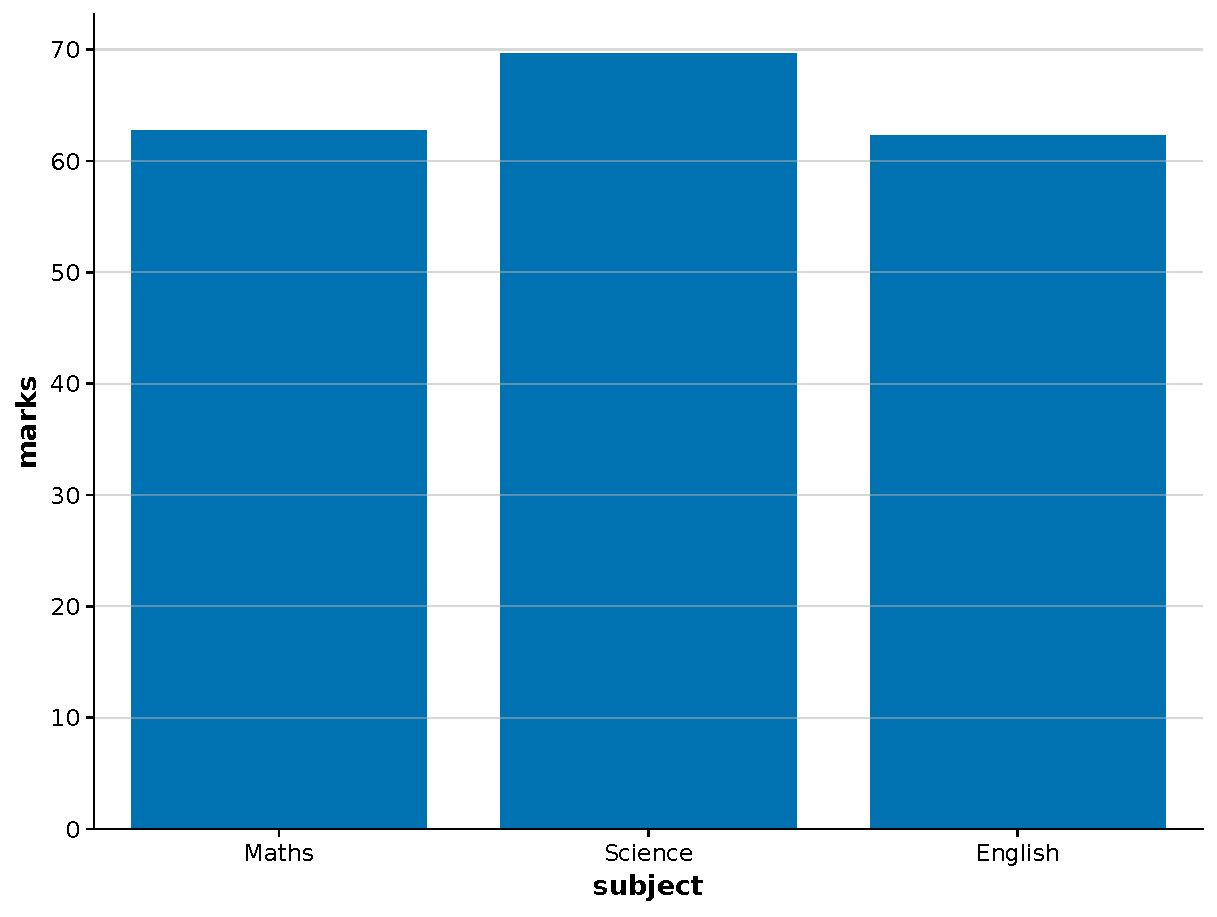
\includegraphics[width=0.52\textwidth,height=0.30\textheight,keepaspectratio]{figures/solution01_task1_lesson1_subjects.pdf}
\captionof*{figure}{Lesson 1, task 1: \code{lesson1\_\allowbreak{}subjects.\allowbreak{}png}.}
\end{minipage}\end{center}
\solutionanswer{Each bar is now one subject, as tall as the average mark of all 18 children in that subject.}
\solutiontask{2}{Save the chart as \code{\textquotedbl{}my\_\allowbreak{}first\_\allowbreak{}chart.\allowbreak{}png\textquotedbl{}} and also as \code{\textquotedbl{}my\_\allowbreak{}first\_\allowbreak{}chart.\allowbreak{}pdf\textquotedbl{}}.}
\begin{lstlisting}[style=py]
import simplydata as sdata
marks = sdata.get_example("marks")
chart = sdata.chart(marks)
chart.draw_bars(x="name", y="marks")
chart.save("my_first_chart.png")
chart.save("my_first_chart.pdf")
\end{lstlisting}
\printedoutput{output/solution01_task2.txt}
\begin{center}\begin{minipage}{\linewidth}\centering
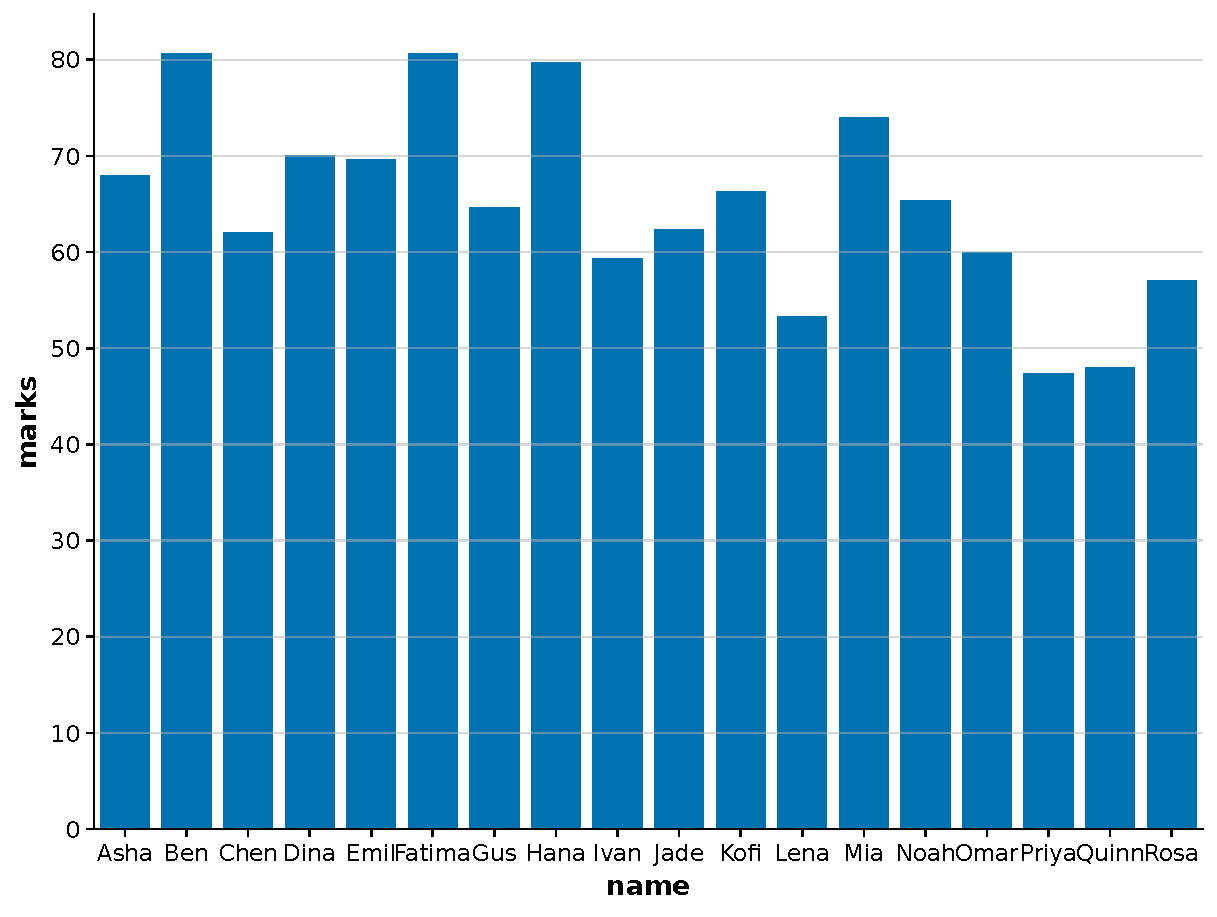
\includegraphics[width=0.52\textwidth,height=0.30\textheight,keepaspectratio]{figures/solution01_task2_my_first_chart.pdf}
\captionof*{figure}{Lesson 1, task 2: \code{my\_\allowbreak{}first\_\allowbreak{}chart.\allowbreak{}png}.}
\end{minipage}\end{center}
\solutionanswer{One chart can be saved many times; the end of the file name (\code{.\allowbreak{}png} or \code{.\allowbreak{}pdf}) decides the type.}
\solutiontask{3}{Make a chart of the \code{\textquotedbl{}fruit\textquotedbl{}} table: bars with \code{x=\textquotedbl{}fruit\textquotedbl{}} and \code{y=\textquotedbl{}count\textquotedbl{}}.}
\begin{lstlisting}[style=py]
import simplydata as sdata
fruit = sdata.get_example("fruit")
chart = sdata.chart(fruit)
chart.draw_bars(x="fruit", y="count")
chart.save("fruit.png")
\end{lstlisting}
\printedoutput{output/solution01_task3.txt}
\begin{center}\begin{minipage}{\linewidth}\centering
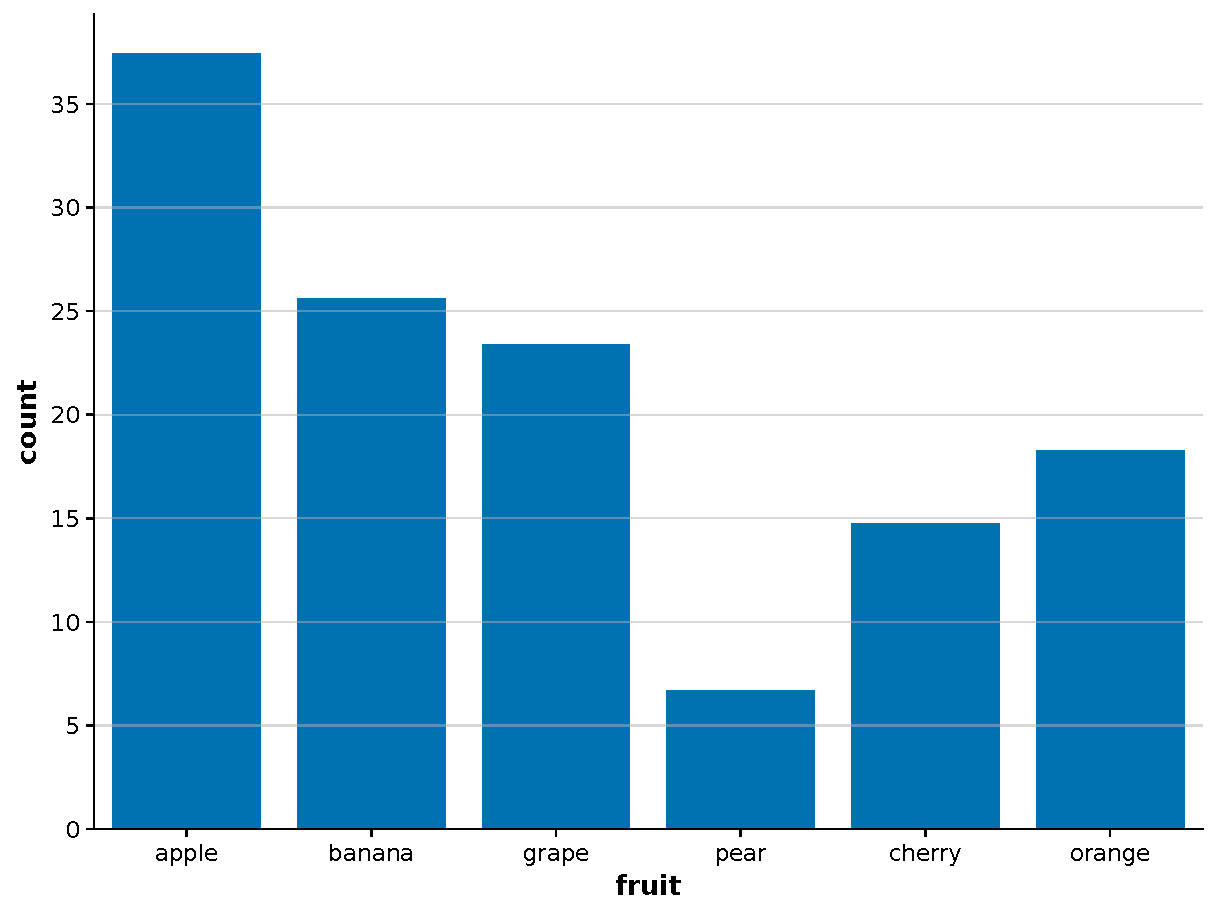
\includegraphics[width=0.52\textwidth,height=0.30\textheight,keepaspectratio]{figures/solution01_task3_fruit.pdf}
\captionof*{figure}{Lesson 1, task 3: \code{fruit.\allowbreak{}png}.}
\end{minipage}\end{center}
\solutionanswer{One bar per fruit. Each fruit was sold several times, so a bar is the average count of one sale; \code{show=\textquotedbl{}total\textquotedbl{}} would show how many were sold in the whole week.}
\par\noindent{\small\sffamily\hyperref[lesson:1]{Back to lesson 1}}
\unsection{Lesson 2: Titles and labels}{solutions:2}
\solutiontask{1}{Give the chart your own title, and label the y-axis \code{\textquotedbl{}Marks out of 100\textquotedbl{}}.}
\begin{lstlisting}[style=py]
import simplydata as sdata
marks = sdata.get_example("marks")
chart = sdata.chart(marks)
chart.draw_bars(x="name", y="marks")
chart.write_title_on_top("How well did each child do?")
chart.label_y("Marks out of 100")
chart.rotate_labels_x(45)
chart.save("lesson2_my_title.png")
\end{lstlisting}
\printedoutput{output/solution02_task1.txt}
\begin{center}\begin{minipage}{\linewidth}\centering
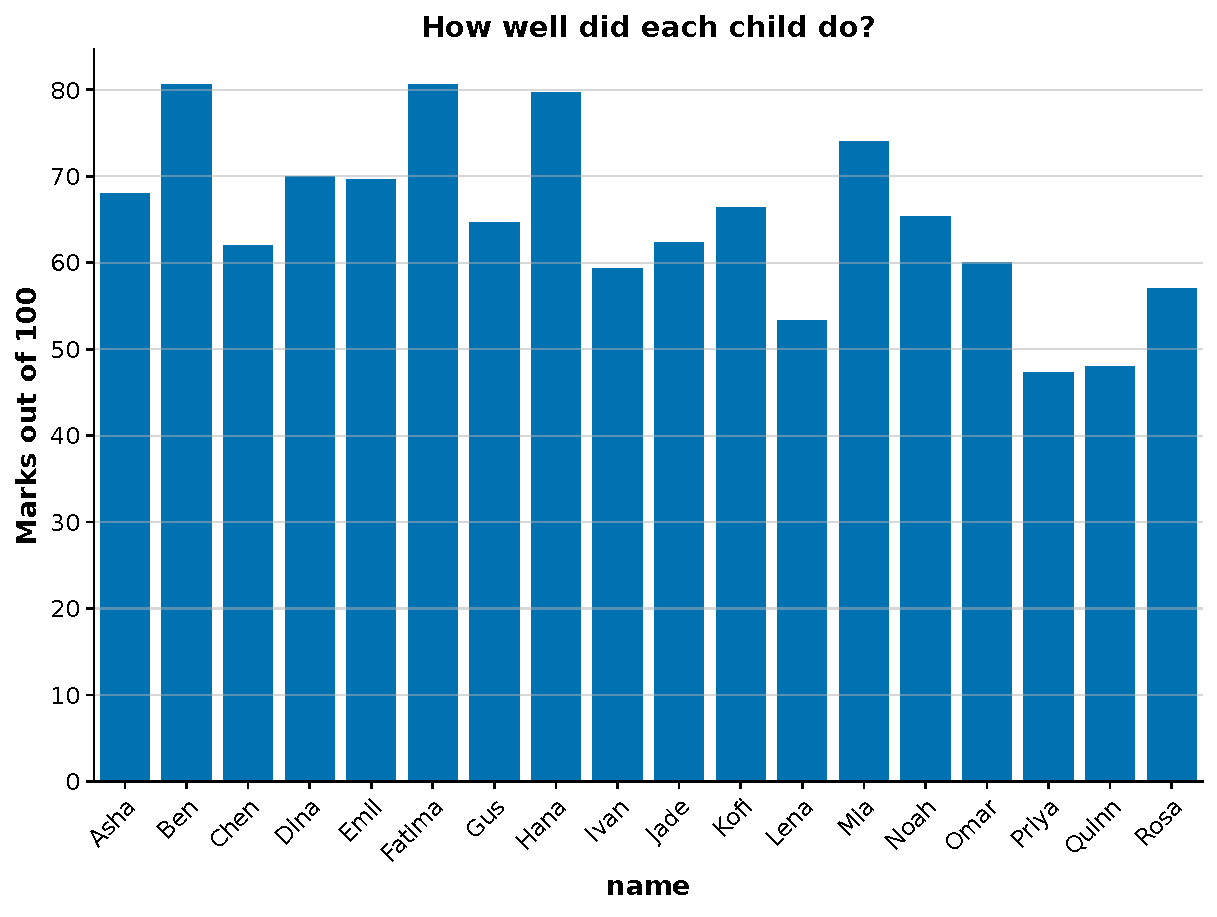
\includegraphics[width=0.52\textwidth,height=0.30\textheight,keepaspectratio]{figures/solution02_task1_lesson2_my_title.pdf}
\captionof*{figure}{Lesson 2, task 1: \code{lesson2\_\allowbreak{}my\_\allowbreak{}title.\allowbreak{}png}.}
\end{minipage}\end{center}
\solutionanswer{\code{write\_\allowbreak{}title\_\allowbreak{}on\_\allowbreak{}top} writes any title you like, and \code{label\_\allowbreak{}y} names the y-axis.}
\solutiontask{2}{Try \code{chart.\allowbreak{}use\_\allowbreak{}font\_\allowbreak{}size(20)}. Then try 9. Which is easier to read?}
\begin{lstlisting}[style=py]
import simplydata as sdata
marks = sdata.get_example("marks")
chart = sdata.chart(marks)
chart.draw_bars(x="name", y="marks")
chart.write_title_on_top("Our class marks")
chart.rotate_labels_x(45)
chart.use_font_size(20)
chart.save("lesson2_big_text.png")
chart.use_font_size(9)
chart.save("lesson2_small_text.png")
\end{lstlisting}
\printedoutput{output/solution02_task2.txt}
\begin{center}\begin{minipage}{\linewidth}\centering
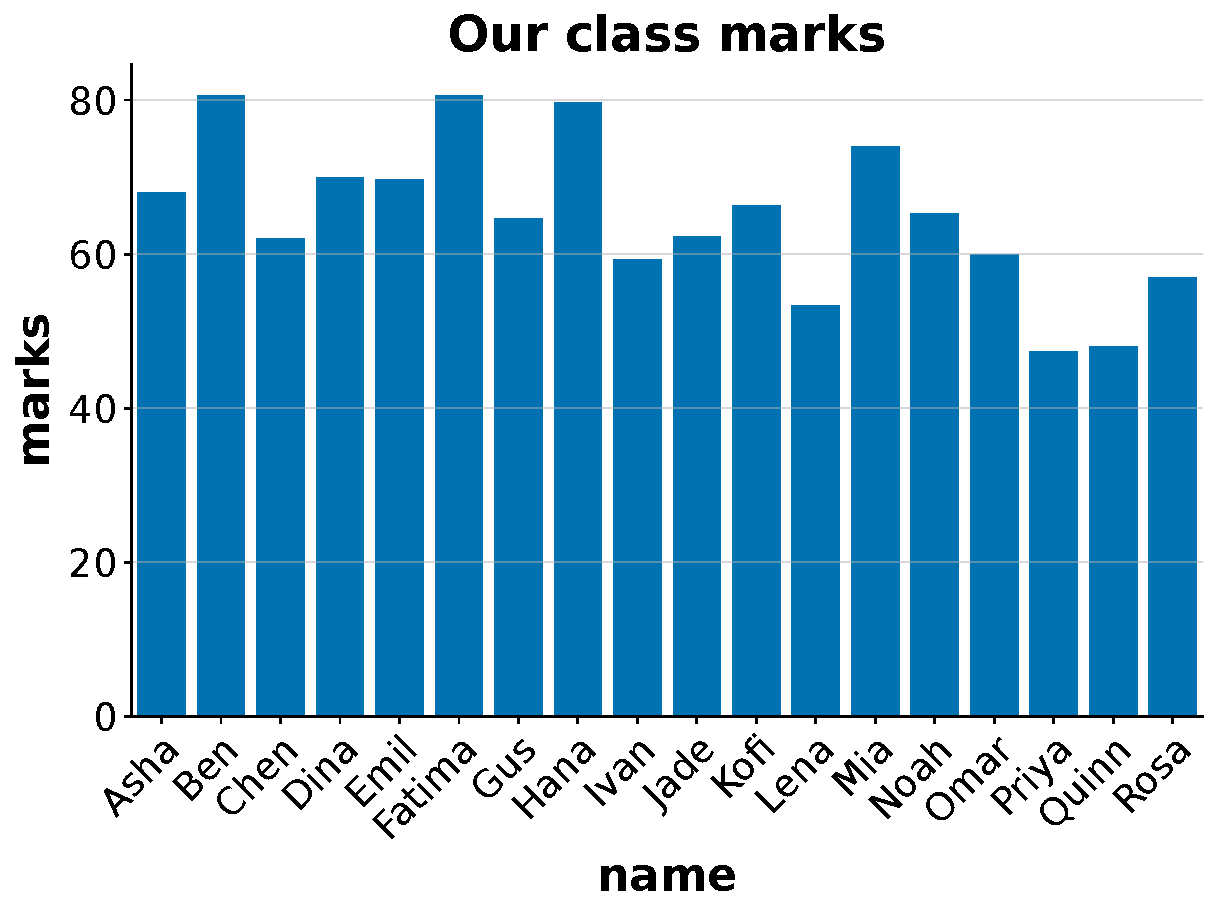
\includegraphics[width=0.48\textwidth,height=0.30\textheight,keepaspectratio]{figures/solution02_task2_lesson2_big_text.pdf}\hfill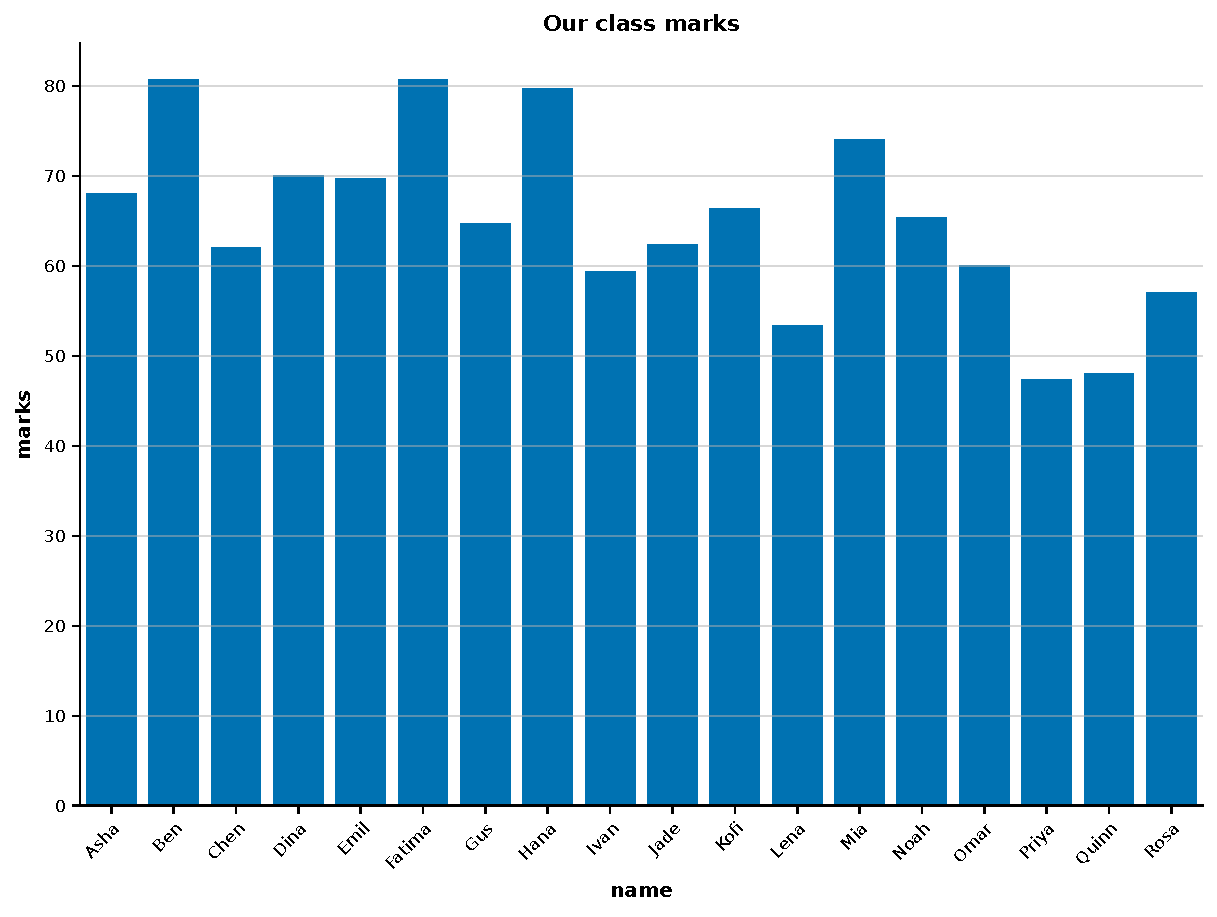
\includegraphics[width=0.48\textwidth,height=0.30\textheight,keepaspectratio]{figures/solution02_task2_lesson2_small_text.pdf}
\captionof*{figure}{Lesson 2, task 2: \code{lesson2\_\allowbreak{}big\_\allowbreak{}text.\allowbreak{}png} and \code{lesson2\_\allowbreak{}small\_\allowbreak{}text.\allowbreak{}png}.}
\end{minipage}\end{center}
\solutionanswer{The last \code{use\_\allowbreak{}font\_\allowbreak{}size} wins, so one chart gives both pictures. Size 20 is easy to read on a slide but crowds the names; 9 fits everything but is small. 12 to 14 suits most charts.}
\solutiontask{3}{Take away the line \code{chart.\allowbreak{}rotate\_\allowbreak{}labels\_\allowbreak{}x(45)}. What happens to the names?}
\begin{lstlisting}[style=py]
import simplydata as sdata
marks = sdata.get_example("marks")
chart = sdata.chart(marks)
chart.draw_bars(x="name", y="marks")
chart.write_title_on_top("Our class marks")
chart.save("lesson2_no_rotate.png")
\end{lstlisting}
\printedoutput{output/solution02_task3.txt}
\begin{center}\begin{minipage}{\linewidth}\centering
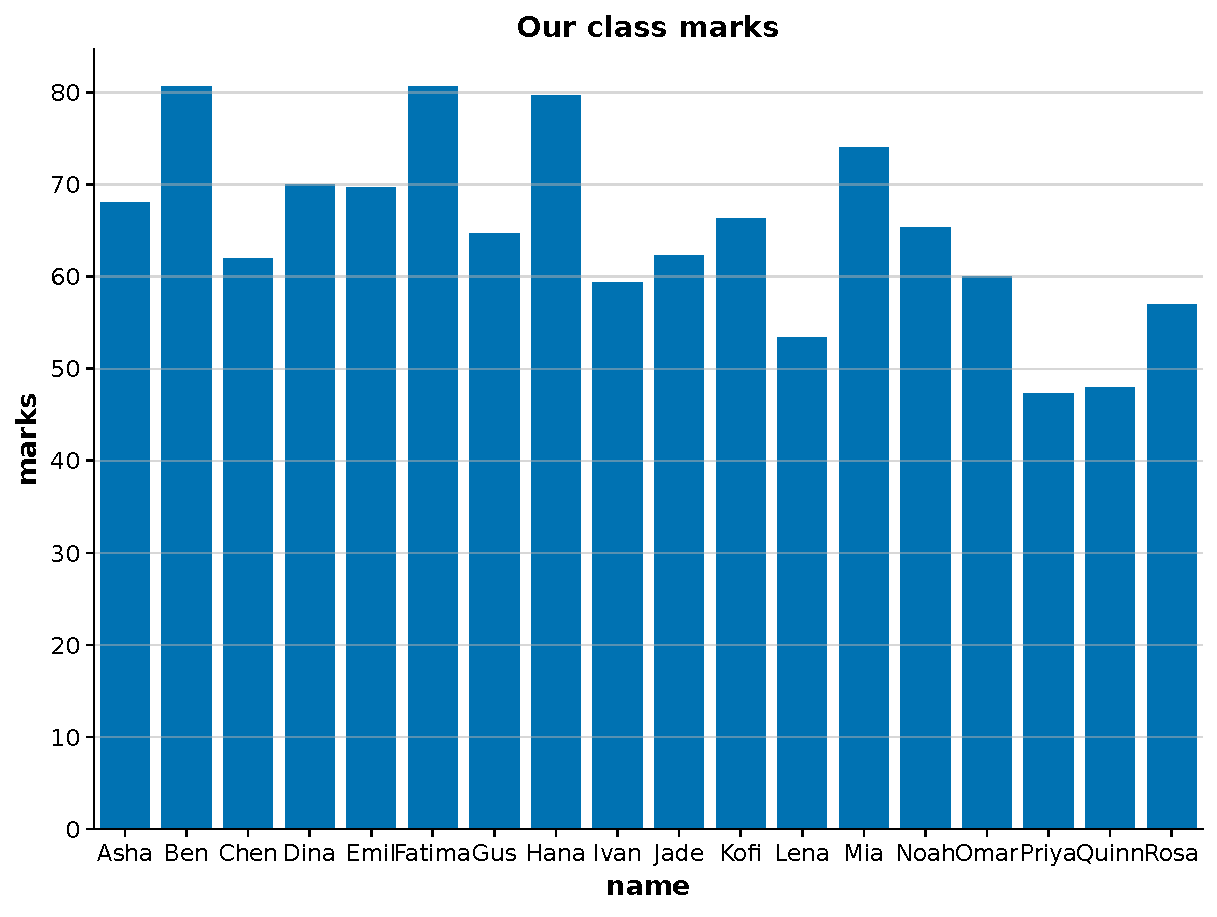
\includegraphics[width=0.52\textwidth,height=0.30\textheight,keepaspectratio]{figures/solution02_task3_lesson2_no_rotate.pdf}
\captionof*{figure}{Lesson 2, task 3: \code{lesson2\_\allowbreak{}no\_\allowbreak{}rotate.\allowbreak{}png}.}
\end{minipage}\end{center}
\solutionanswer{Without \code{rotate\_\allowbreak{}labels\_\allowbreak{}x} the 18 names lie flat under the bars and run into each other.}
\par\noindent{\small\sffamily\hyperref[lesson:2]{Back to lesson 2}}
\unsection{Lesson 3: Colours, groups and legends}{solutions:3}
\solutiontask{1}{In the weather chart, add \code{colour=\textquotedbl{}city\textquotedbl{}} to \code{chart.\allowbreak{}draw\_\allowbreak{}lines(.\allowbreak{}.\allowbreak{}.\allowbreak{})}. How many lines do you get?}
\begin{lstlisting}[style=py]
import simplydata as sdata
weather = sdata.get_example("weather")
chart = sdata.chart(weather)
chart.draw_lines(x="month", y="rain", colour="city")
chart.save("lesson3_cities.png")
\end{lstlisting}
\printedoutput{output/solution03_task1.txt}
\begin{center}\begin{minipage}{\linewidth}\centering
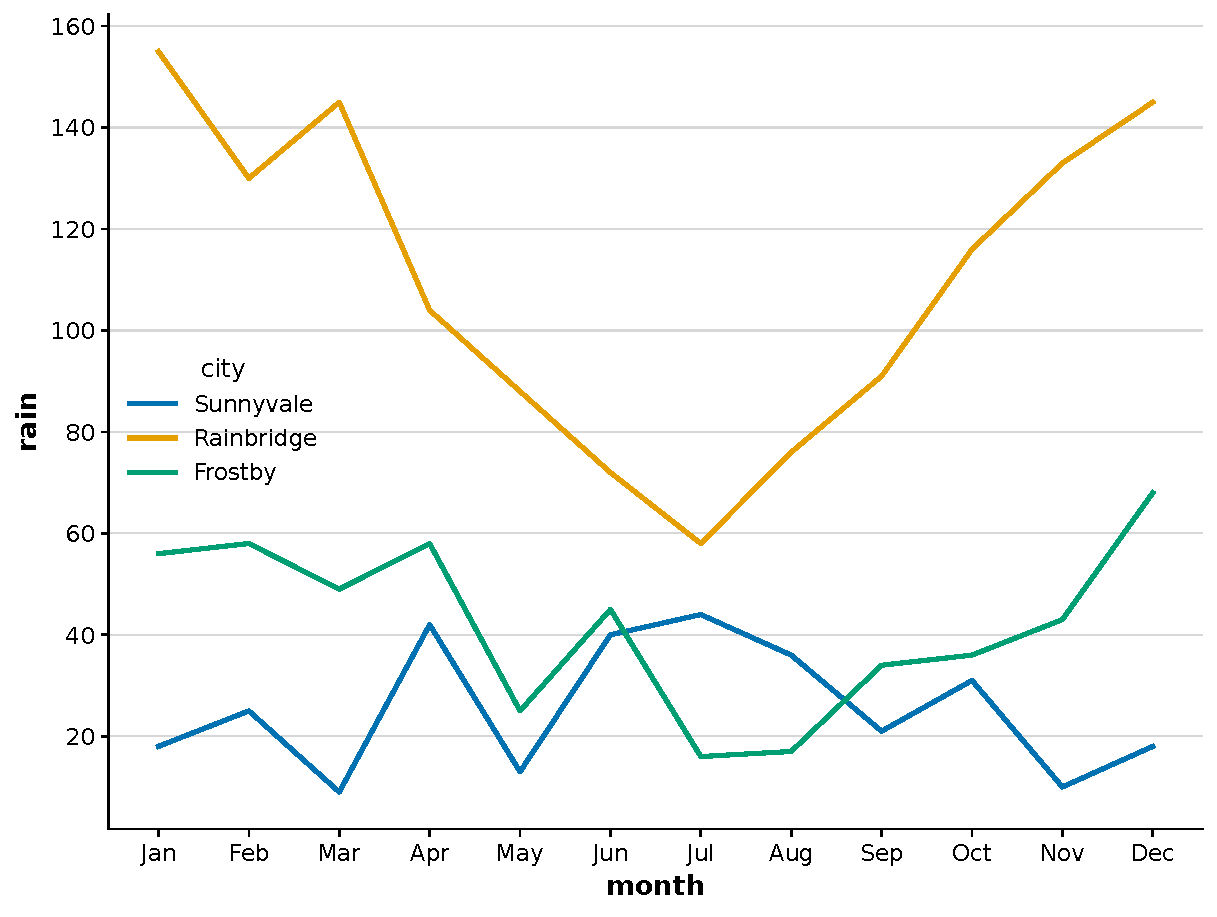
\includegraphics[width=0.52\textwidth,height=0.30\textheight,keepaspectratio]{figures/solution03_task1_lesson3_cities.pdf}
\captionof*{figure}{Lesson 3, task 1: \code{lesson3\_\allowbreak{}cities.\allowbreak{}png}.}
\end{minipage}\end{center}
\solutionanswer{Three lines, one for each city, and a legend that says which colour is which city.}
\solutiontask{2}{Move the legend to the top with \code{chart.\allowbreak{}put\_\allowbreak{}legend\_\allowbreak{}at\_\allowbreak{}top()}.}
\begin{lstlisting}[style=py]
import simplydata as sdata
marks = sdata.get_example("marks")
chart = sdata.chart(marks)
chart.draw_bars(x="subject", y="marks", colour="class")
chart.use_colours("orange", "teal", "purple")
chart.put_legend_at_top()
chart.save("lesson3_legend_top.png")
\end{lstlisting}
\printedoutput{output/solution03_task2.txt}
\begin{center}\begin{minipage}{\linewidth}\centering
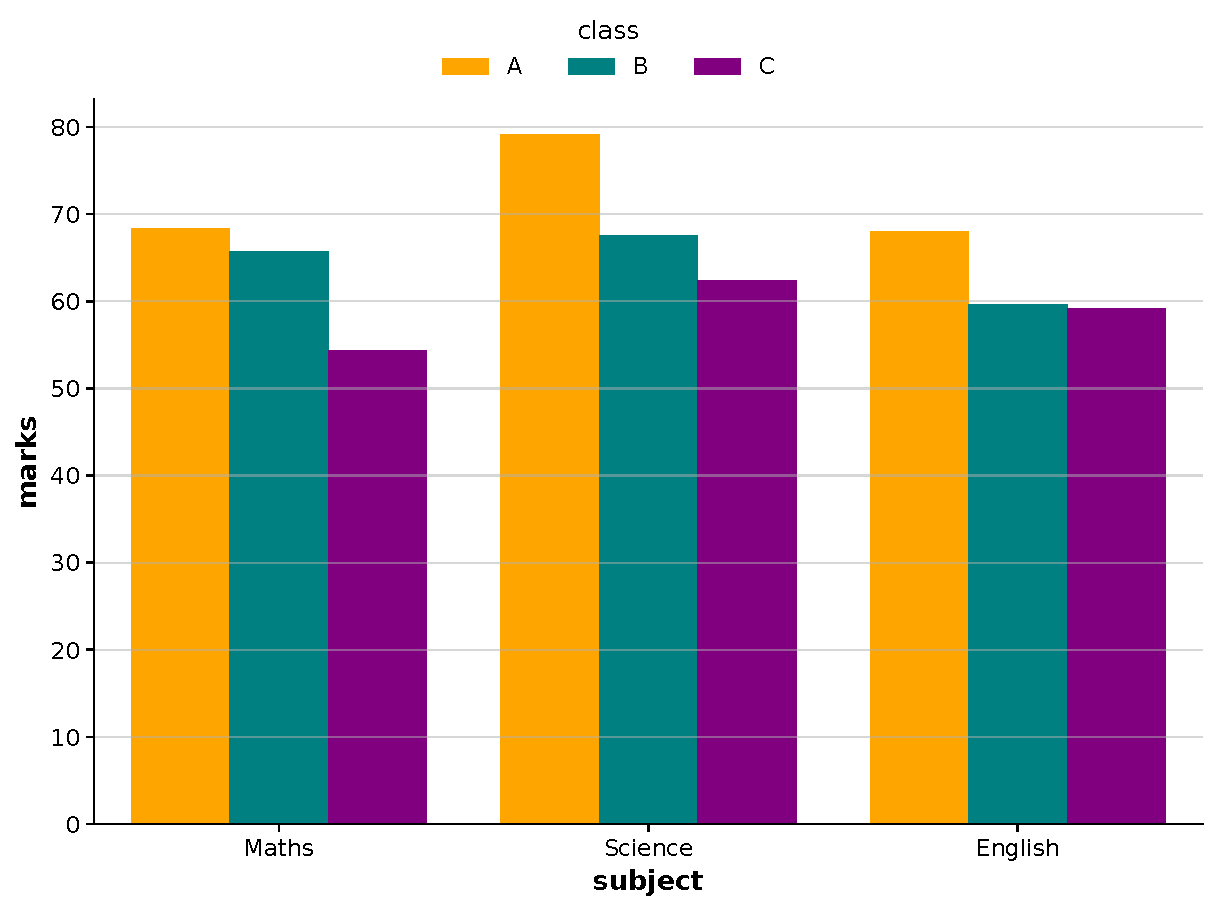
\includegraphics[width=0.52\textwidth,height=0.30\textheight,keepaspectratio]{figures/solution03_task2_lesson3_legend_top.pdf}
\captionof*{figure}{Lesson 3, task 2: \code{lesson3\_\allowbreak{}legend\_\allowbreak{}top.\allowbreak{}png}.}
\end{minipage}\end{center}
\solutionanswer{\code{put\_\allowbreak{}legend\_\allowbreak{}at\_\allowbreak{}top} puts the legend above the chart, in place of \code{put\_\allowbreak{}legend\_\allowbreak{}at\_\allowbreak{}bottom}.}
\solutiontask{3}{Try \code{chart.\allowbreak{}use\_\allowbreak{}style(\textquotedbl{}dark\textquotedbl{})} and choose three colours that look good on it.}
\begin{lstlisting}[style=py]
import simplydata as sdata
marks = sdata.get_example("marks")
chart = sdata.chart(marks)
chart.draw_bars(x="subject", y="marks", colour="class")
chart.use_style("dark")
chart.use_colours("gold", "turquoise", "hotpink")
chart.save("lesson3_dark.png")
\end{lstlisting}
\printedoutput{output/solution03_task3.txt}
\begin{center}\begin{minipage}{\linewidth}\centering
\includegraphics[width=0.52\textwidth,height=0.30\textheight,keepaspectratio]{figures/solution03_task3_lesson3_dark.pdf}
\captionof*{figure}{Lesson 3, task 3: \code{lesson3\_\allowbreak{}dark.\allowbreak{}png}.}
\end{minipage}\end{center}
\solutionanswer{Light, bright colours stand out on a dark background; dark colours such as navy would almost disappear.}
\par\noindent{\small\sffamily\hyperref[lesson:3]{Back to lesson 3}}
\unsection{Lesson 4: Different chart types}{solutions:4}
\solutiontask{1}{Draw \code{chart.\allowbreak{}draw\_\allowbreak{}violins(x=\textquotedbl{}class\textquotedbl{},\allowbreak{} y=\textquotedbl{}marks\textquotedbl{})} instead of boxes. What is different?}
\begin{lstlisting}[style=py]
import simplydata as sdata
marks = sdata.get_example("marks")
chart = sdata.chart(marks)
chart.draw_violins(x="class", y="marks")
chart.draw_all_dots(x="class", y="marks")
chart.save("lesson4_violins.png")
\end{lstlisting}
\printedoutput{output/solution04_task1.txt}
\begin{center}\begin{minipage}{\linewidth}\centering
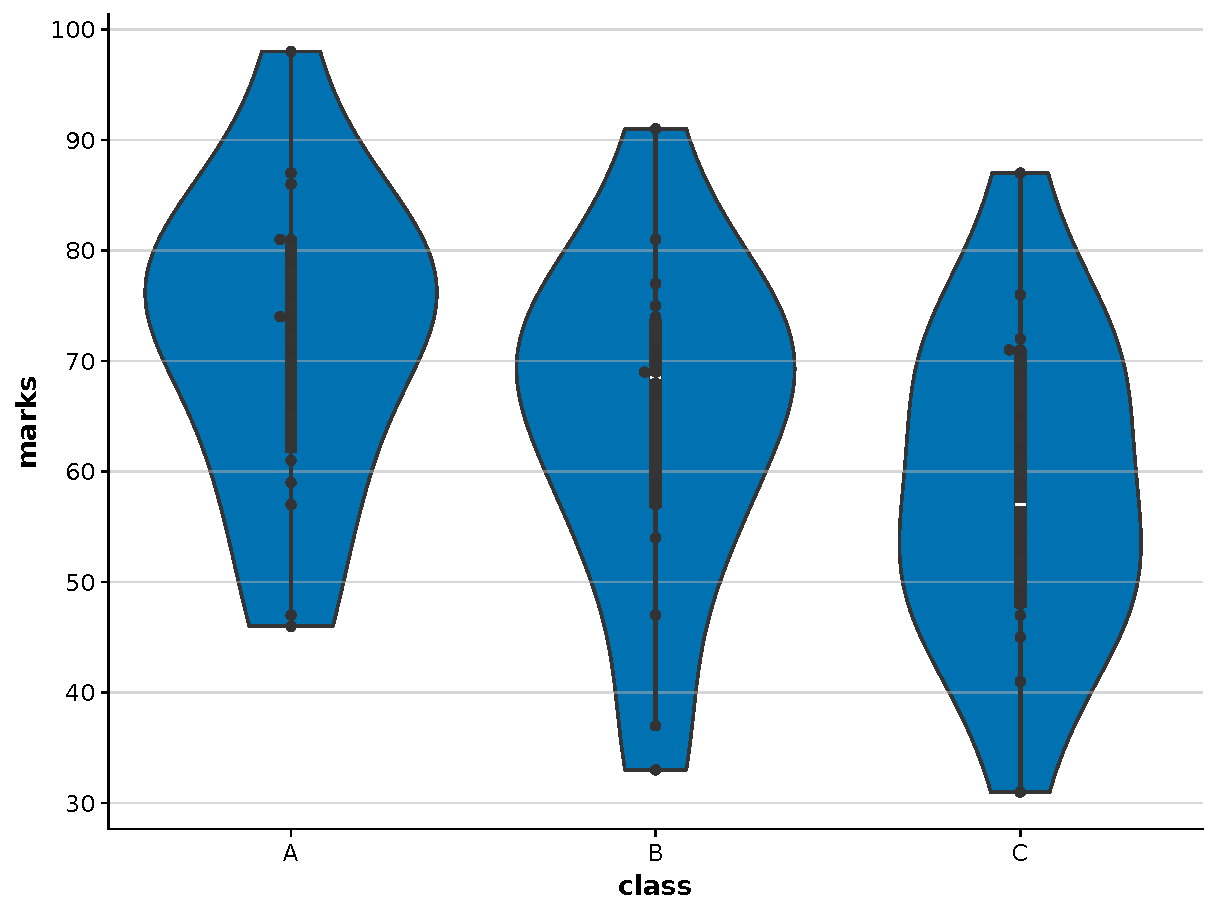
\includegraphics[width=0.52\textwidth,height=0.30\textheight,keepaspectratio]{figures/solution04_task1_lesson4_violins.pdf}
\captionof*{figure}{Lesson 4, task 1: \code{lesson4\_\allowbreak{}violins.\allowbreak{}png}.}
\end{minipage}\end{center}
\solutionanswer{A violin shows the whole shape of the marks: it is wide where many marks are and thin where few are. A box shows only the middle half and the median.}
\solutiontask{2}{Draw a histogram of the weather \code{\textquotedbl{}temperature\textquotedbl{}} column with \code{with\_\allowbreak{}bins=6}.}
\begin{lstlisting}[style=py]
import simplydata as sdata
weather = sdata.get_example("weather")
chart = sdata.chart(weather)
chart.draw_histogram(x="temperature", with_bins=6)
chart.save("lesson4_temperature.png")
\end{lstlisting}
\printedoutput{output/solution04_task2.txt}
\begin{center}\begin{minipage}{\linewidth}\centering
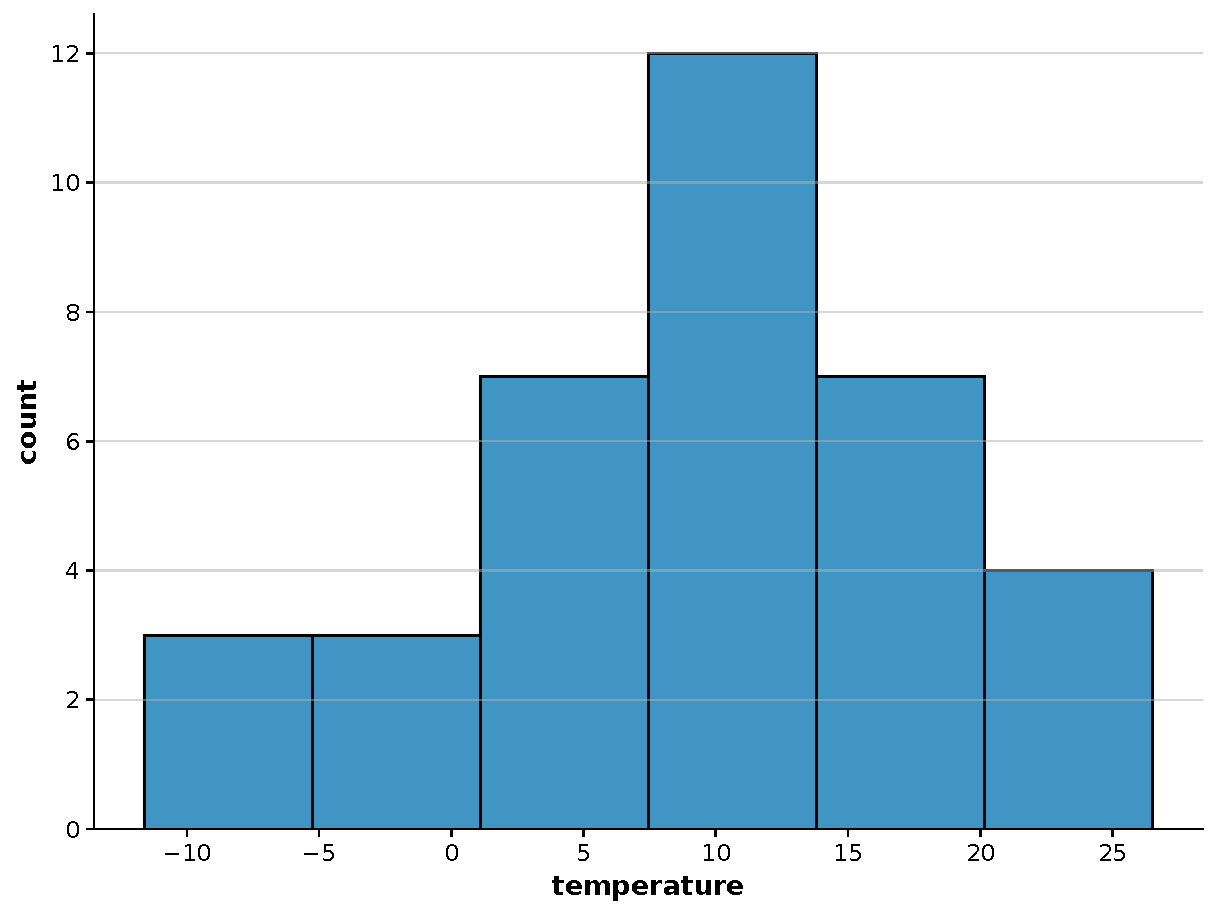
\includegraphics[width=0.52\textwidth,height=0.30\textheight,keepaspectratio]{figures/solution04_task2_lesson4_temperature.pdf}
\captionof*{figure}{Lesson 4, task 2: \code{lesson4\_\allowbreak{}temperature.\allowbreak{}png}.}
\end{minipage}\end{center}
\solutionanswer{Six ranges of temperature, each bar as high as the number of months (of all three cities) that fall in it.}
\solutiontask{3}{Make a chart of \code{sdata.\allowbreak{}get\_\allowbreak{}example(\textquotedbl{}growth\textquotedbl{})} and draw \code{chart.\allowbreak{}draw\_\allowbreak{}area(x=\textquotedbl{}year\textquotedbl{},\allowbreak{} y=\textquotedbl{}population\textquotedbl{},\allowbreak{} colour=\textquotedbl{}country\textquotedbl{})}.}
\begin{lstlisting}[style=py]
import simplydata as sdata
growth = sdata.get_example("growth")
chart = sdata.chart(growth)
chart.draw_area(x="year", y="population", colour="country")
chart.save("lesson4_area.png")
\end{lstlisting}
\printedoutput{output/solution04_task3.txt}
\begin{center}\begin{minipage}{\linewidth}\centering
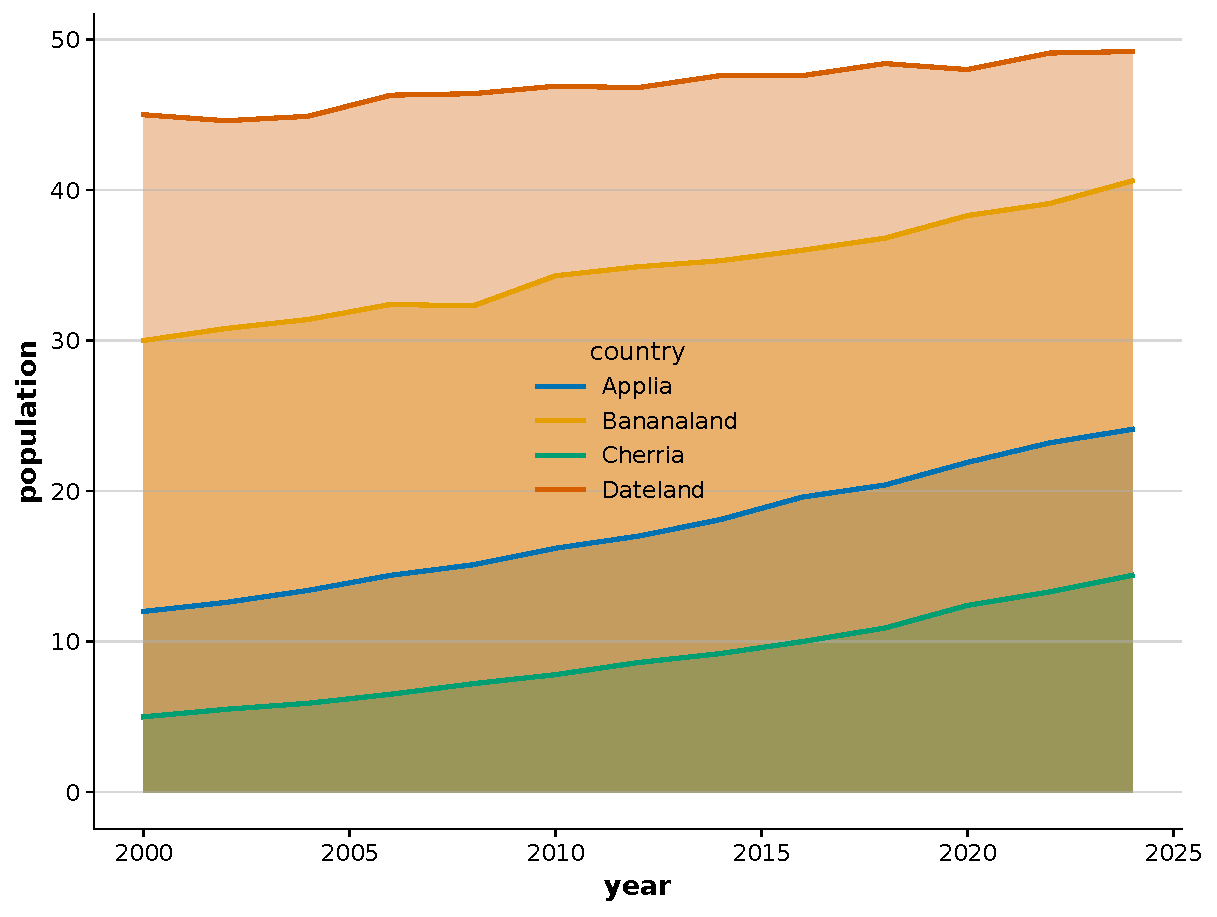
\includegraphics[width=0.52\textwidth,height=0.30\textheight,keepaspectratio]{figures/solution04_task3_lesson4_area.pdf}
\captionof*{figure}{Lesson 4, task 3: \code{lesson4\_\allowbreak{}area.\allowbreak{}png}.}
\end{minipage}\end{center}
\solutionanswer{An area chart is a line chart with the space under each line filled in.}
\par\noindent{\small\sffamily\hyperref[lesson:4]{Back to lesson 4}}
\unsection{Lesson 5: Statistics: averages, error bars and fit lines}{solutions:5}
\solutiontask{1}{Change \code{show=\textquotedbl{}average\textquotedbl{}} to \code{show=\textquotedbl{}median\textquotedbl{}}. Do the bars change much?}
\begin{lstlisting}[style=py]
import simplydata as sdata
marks = sdata.get_example("marks")
chart = sdata.chart(marks)
chart.draw_bars(x="class", y="marks", show="median")
chart.write_numbers_on_bars()
chart.save("lesson5_median.png")
\end{lstlisting}
\printedoutput{output/solution05_task1.txt}
\begin{center}\begin{minipage}{\linewidth}\centering
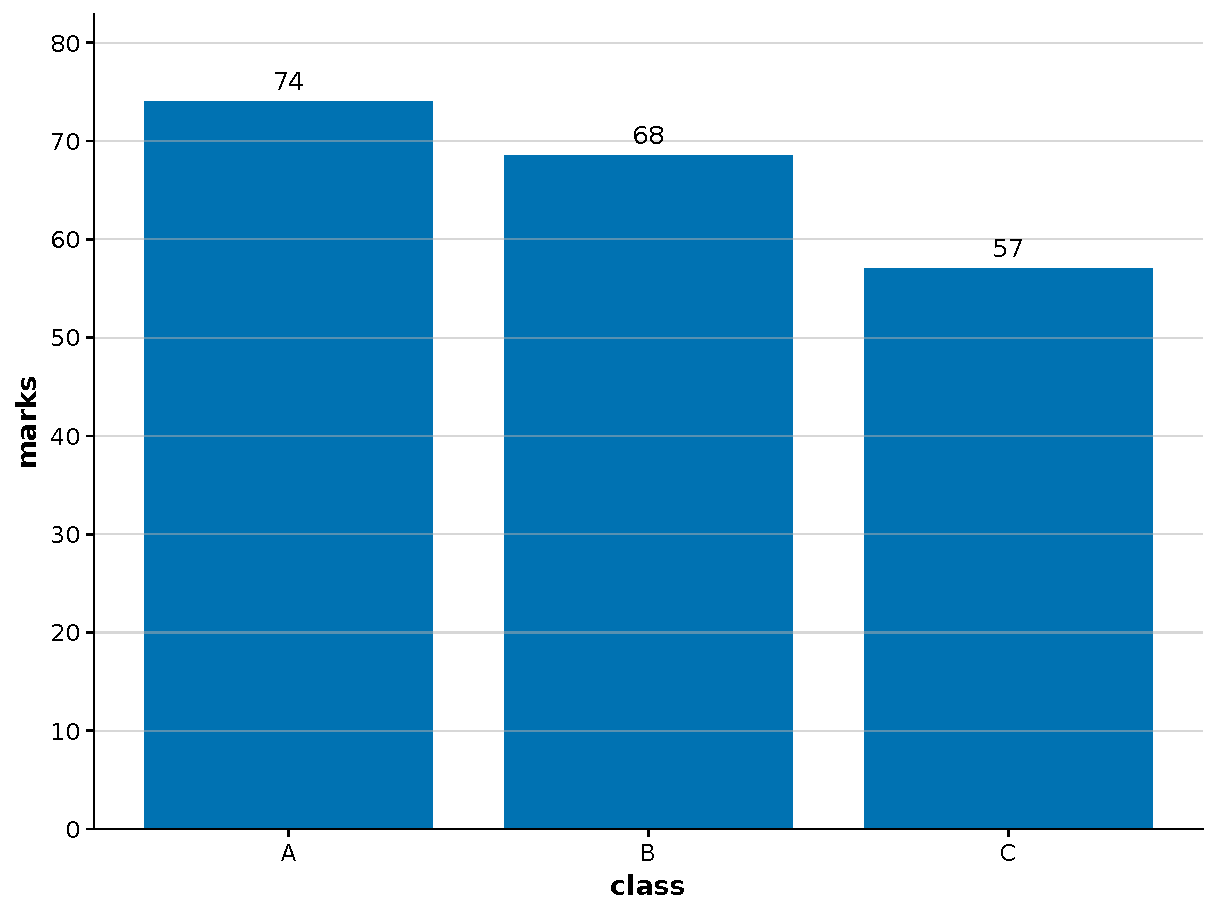
\includegraphics[width=0.52\textwidth,height=0.30\textheight,keepaspectratio]{figures/solution05_task1_lesson5_median.pdf}
\captionof*{figure}{Lesson 5, task 1: \code{lesson5\_\allowbreak{}median.\allowbreak{}png}.}
\end{minipage}\end{center}
\solutionanswer{Error bars go with averages, so \code{error=} comes out. The medians (A 74, B 68.5, C 57) are close to the averages (A 71.8, B 64.3, C 58.6): no single mark pulls them far.}
\solutiontask{2}{Change \code{error=\textquotedbl{}standard deviation\textquotedbl{}} to \code{error=\textquotedbl{}standard error\textquotedbl{}}. Are the error bars bigger or smaller? Why?}
\begin{lstlisting}[style=py]
import simplydata as sdata
marks = sdata.get_example("marks")
chart = sdata.chart(marks)
chart.draw_bars(x="class", y="marks", show="average", error="standard error")
chart.save("lesson5_standard_error.png")
\end{lstlisting}
\printedoutput{output/solution05_task2.txt}
\begin{center}\begin{minipage}{\linewidth}\centering
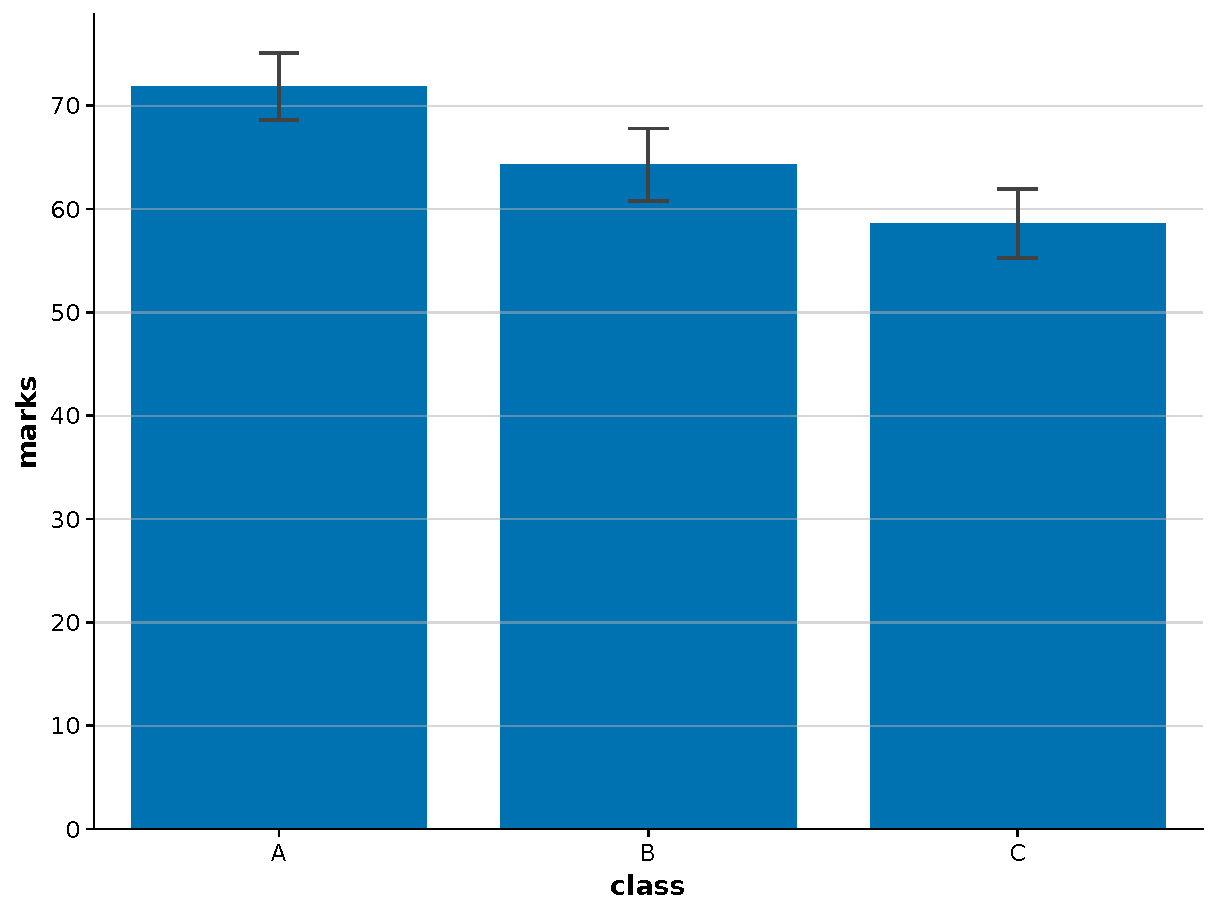
\includegraphics[width=0.52\textwidth,height=0.30\textheight,keepaspectratio]{figures/solution05_task2_lesson5_standard_error.pdf}
\captionof*{figure}{Lesson 5, task 2: \code{lesson5\_\allowbreak{}standard\_\allowbreak{}error.\allowbreak{}png}.}
\end{minipage}\end{center}
\solutionanswer{Smaller: the standard error is the standard deviation divided by the square root of the number of values (here 18), so it is about a quarter of the standard deviation.}
\solutiontask{3}{Make a chart of the weather table, draw dots with \code{x=\textquotedbl{}month\_\allowbreak{}number\textquotedbl{}}, \code{y=\textquotedbl{}temperature\textquotedbl{}} and add \code{chart.\allowbreak{}fit\_\allowbreak{}curve(of\_\allowbreak{}degree=2)}.}
\begin{lstlisting}[style=py]
import simplydata as sdata
weather = sdata.get_example("weather")
chart = sdata.chart(weather)
chart.draw_dots(x="month_number", y="temperature", colour="city")
chart.fit_curve(of_degree=2)
chart.save("lesson5_fit_curve.png")
\end{lstlisting}
\printedoutput{output/solution05_task3.txt}
\begin{center}\begin{minipage}{\linewidth}\centering
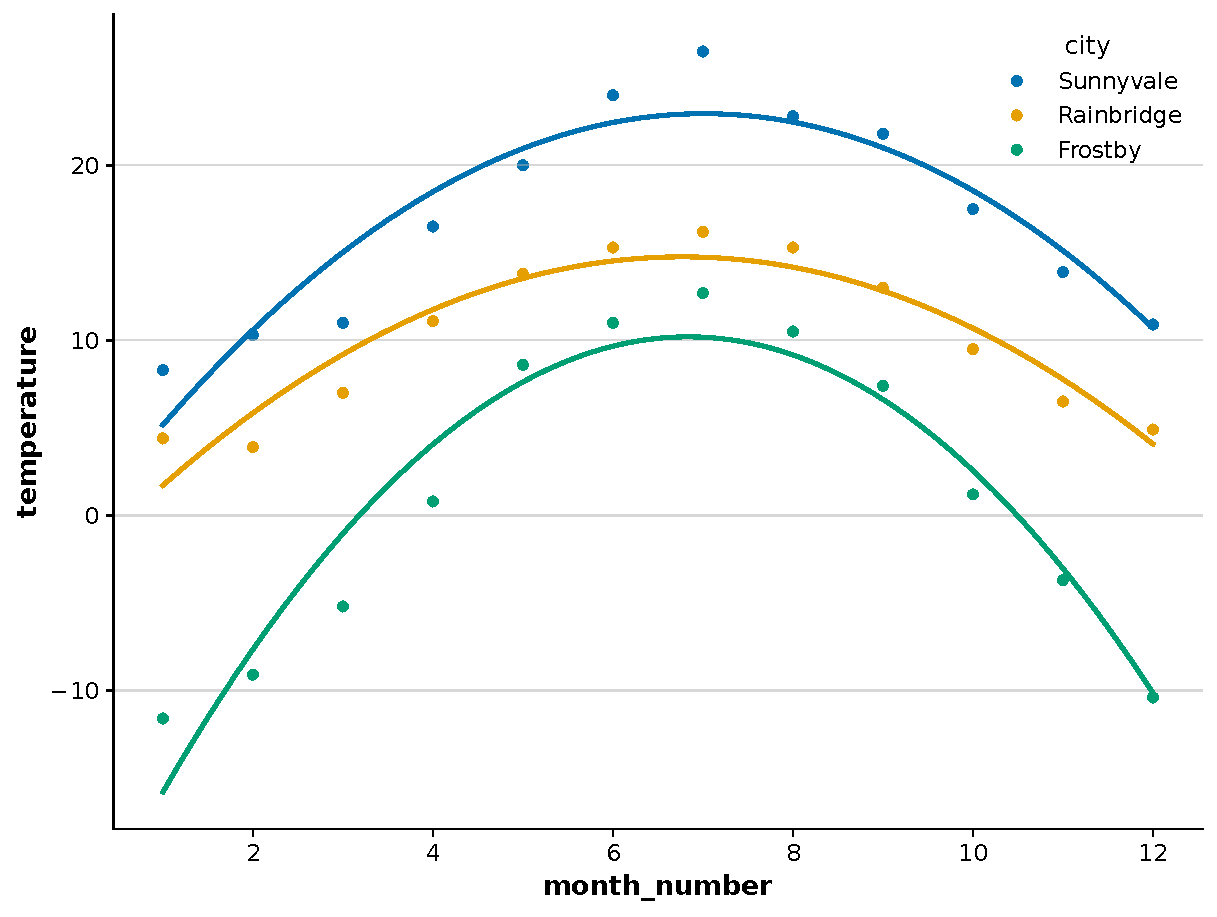
\includegraphics[width=0.52\textwidth,height=0.30\textheight,keepaspectratio]{figures/solution05_task3_lesson5_fit_curve.pdf}
\captionof*{figure}{Lesson 5, task 3: \code{lesson5\_\allowbreak{}fit\_\allowbreak{}curve.\allowbreak{}png}.}
\end{minipage}\end{center}
\solutionanswer{Each city gets a curve with one bend: warm in the middle of the year, cold at both ends.}
\par\noindent{\small\sffamily\hyperref[lesson:5]{Back to lesson 5}}
\unsection{Lesson 6: Axes and reference lines}{solutions:6}
\solutiontask{1}{Move the pass mark to 60 and shade between 0 and 40 instead.}
\begin{lstlisting}[style=py]
import simplydata as sdata
marks = sdata.get_example("marks")
chart = sdata.chart(marks)
chart.draw_bars(x="name", y="marks")
chart.set_range_y(0, 100)
chart.draw_line_at_y(60, labelled="pass mark")
chart.shade_between_y(0, 40)
chart.rotate_labels_x()
chart.save("lesson6_pass_60.png")
\end{lstlisting}
\printedoutput{output/solution06_task1.txt}
\begin{center}\begin{minipage}{\linewidth}\centering
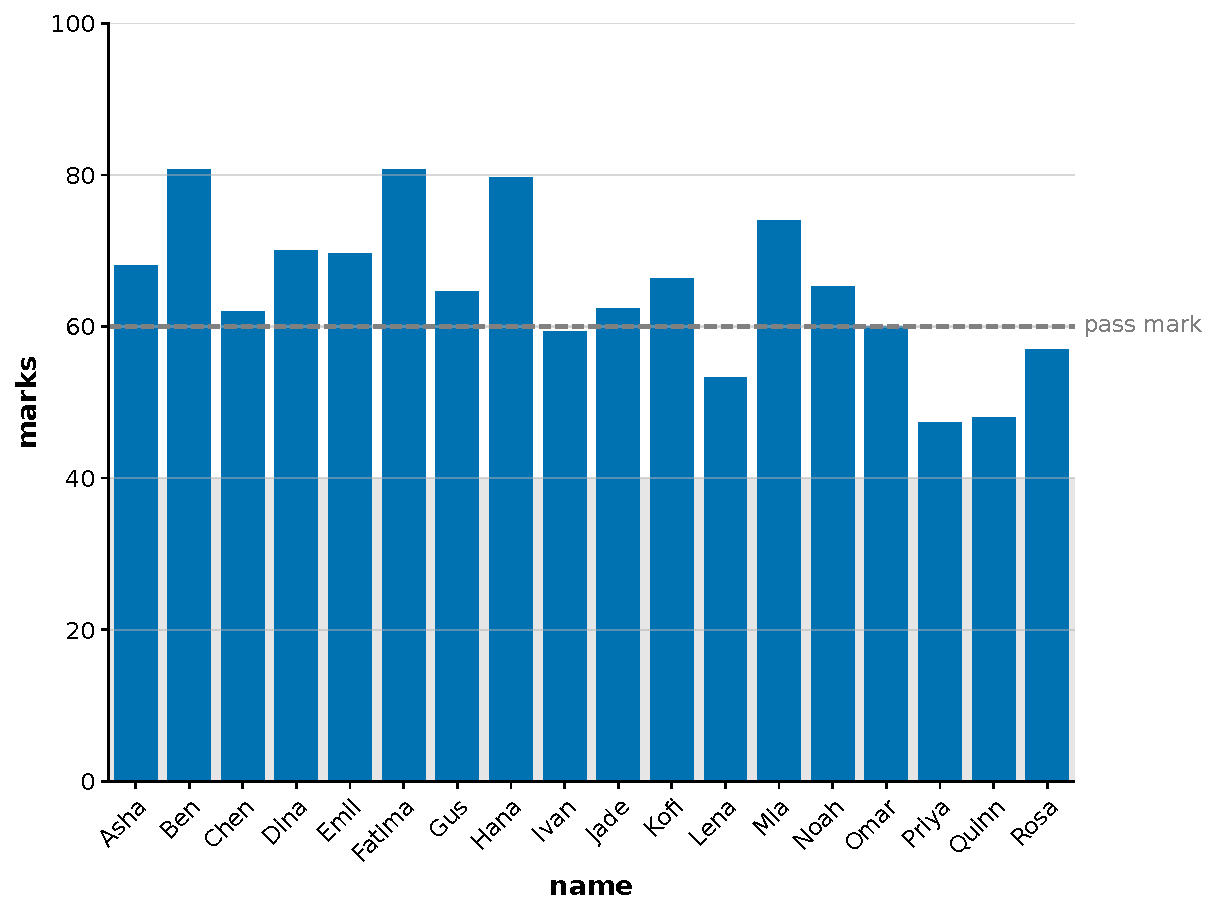
\includegraphics[width=0.52\textwidth,height=0.30\textheight,keepaspectratio]{figures/solution06_task1_lesson6_pass_60.pdf}
\captionof*{figure}{Lesson 6, task 1: \code{lesson6\_\allowbreak{}pass\_\allowbreak{}60.\allowbreak{}png}.}
\end{minipage}\end{center}
\solutionanswer{\code{draw\_\allowbreak{}line\_\allowbreak{}at\_\allowbreak{}y(60)} moves the line; \code{shade\_\allowbreak{}between\_\allowbreak{}y(0,\allowbreak{} 40)} shades the band from 0 to 40.}
\solutiontask{2}{Take away \code{chart.\allowbreak{}use\_\allowbreak{}log\_\allowbreak{}scale\_\allowbreak{}y()}. Which countries look different?}
\begin{lstlisting}[style=py]
import simplydata as sdata
growth = sdata.get_example("growth")
chart = sdata.chart(growth)
chart.draw_lines(x="year", y="population", colour="country")
chart.draw_line_at_x(2010, labelled="2010")
chart.label_y("People (millions)")
chart.save("lesson6_no_log.png")
\end{lstlisting}
\printedoutput{output/solution06_task2.txt}
\begin{center}\begin{minipage}{\linewidth}\centering
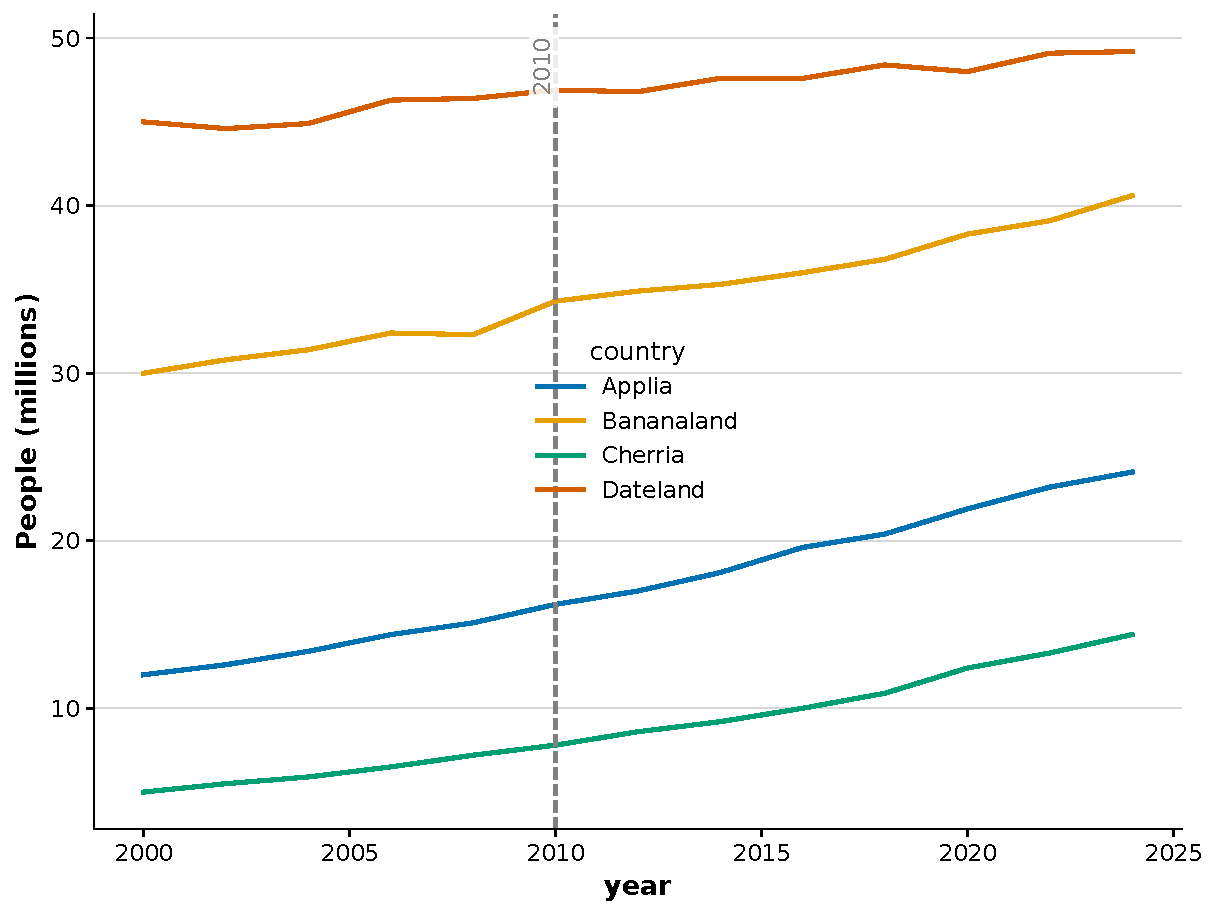
\includegraphics[width=0.52\textwidth,height=0.30\textheight,keepaspectratio]{figures/solution06_task2_lesson6_no_log.pdf}
\captionof*{figure}{Lesson 6, task 2: \code{lesson6\_\allowbreak{}no\_\allowbreak{}log.\allowbreak{}png}.}
\end{minipage}\end{center}
\solutionanswer{The lines now bend upwards instead of running straight, and the small countries (Cherria and Applia) sit low and look flat, although Cherria nearly triples.}
\solutiontask{3}{Try \code{chart.\allowbreak{}flip\_\allowbreak{}y()} on any chart. What happens?}
\begin{lstlisting}[style=py]
import simplydata as sdata
marks = sdata.get_example("marks")
chart = sdata.chart(marks)
chart.draw_bars(x="class", y="marks")
chart.flip_y()
chart.save("lesson6_flip.png")
\end{lstlisting}
\printedoutput{output/solution06_task3.txt}
\begin{center}\begin{minipage}{\linewidth}\centering
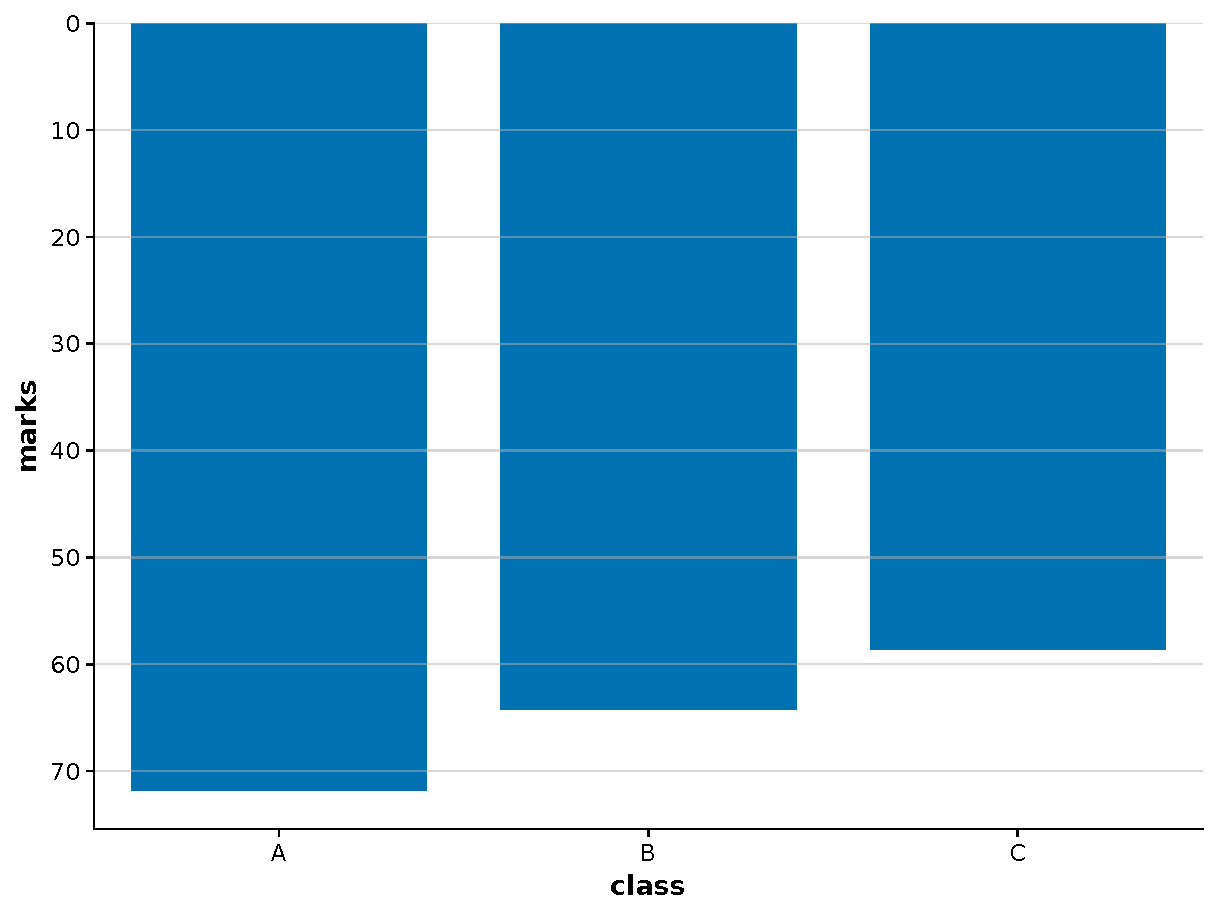
\includegraphics[width=0.52\textwidth,height=0.30\textheight,keepaspectratio]{figures/solution06_task3_lesson6_flip.pdf}
\captionof*{figure}{Lesson 6, task 3: \code{lesson6\_\allowbreak{}flip.\allowbreak{}png}.}
\end{minipage}\end{center}
\solutionanswer{The y-axis turns upside down: 0 is at the top and the bars hang down. Useful for depths, where bigger numbers are further down.}
\par\noindent{\small\sffamily\hyperref[lesson:6]{Back to lesson 6}}
\unsection{Lesson 7: Several charts together}{solutions:7}
\solutiontask{1}{Change \code{chart.\allowbreak{}draw\_\allowbreak{}one\_\allowbreak{}chart\_\allowbreak{}for\_\allowbreak{}each\_\allowbreak{}group\_\allowbreak{}in(\textquotedbl{}class\textquotedbl{})} to \code{chart.\allowbreak{}draw\_\allowbreak{}one\_\allowbreak{}chart\_\allowbreak{}for\_\allowbreak{}each\_\allowbreak{}group\_\allowbreak{}in(\textquotedbl{}subject\textquotedbl{})}.}
\begin{lstlisting}[style=py]
import simplydata as sdata
marks = sdata.get_example("marks")
chart = sdata.chart(marks)
chart.draw_dots(x="hours", y="marks")
chart.fit_line()
chart.draw_one_chart_for_each_group_in("subject")
chart.save("lesson7_per_subject.png")
\end{lstlisting}
\printedoutput{output/solution07_task1.txt}
\begin{center}\begin{minipage}{\linewidth}\centering
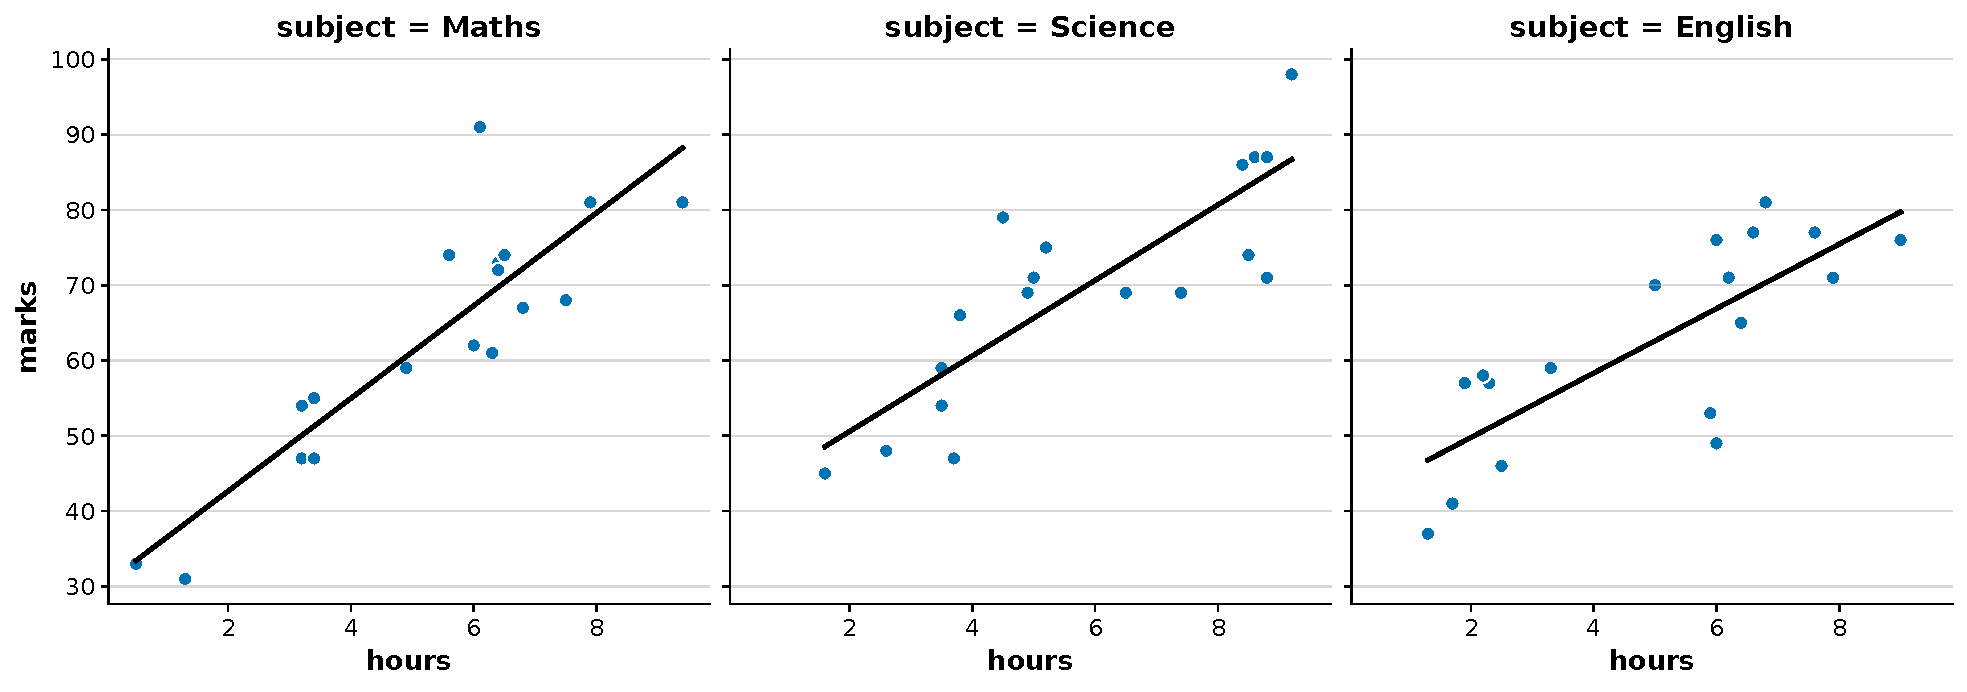
\includegraphics[width=0.52\textwidth,height=0.30\textheight,keepaspectratio]{figures/solution07_task1_lesson7_per_subject.pdf}
\captionof*{figure}{Lesson 7, task 1: \code{lesson7\_\allowbreak{}per\_\allowbreak{}subject.\allowbreak{}png}.}
\end{minipage}\end{center}
\solutionanswer{One small chart for each subject (Maths, Science and English), each with its own fit line.}
\solutiontask{2}{Use \code{sdata.\allowbreak{}put\_\allowbreak{}side\_\allowbreak{}by\_\allowbreak{}side(a,\allowbreak{} b)} instead of \code{sdata.\allowbreak{}put\_\allowbreak{}one\_\allowbreak{}above\_\allowbreak{}other(a,\allowbreak{} b)} for the weather charts.}
\begin{lstlisting}[style=py]
import simplydata as sdata
weather = sdata.get_example("weather")
a = sdata.chart(weather).draw_lines(x="month", y="temperature", colour="city")
b = sdata.chart(weather).draw_bars(x="month", y="rain", colour="city")
page = sdata.put_side_by_side(a, b)
page.write_title_on_top("A year of weather")
page.save("lesson7_side_by_side.png")
\end{lstlisting}
\printedoutput{output/solution07_task2.txt}
\begin{center}\begin{minipage}{\linewidth}\centering
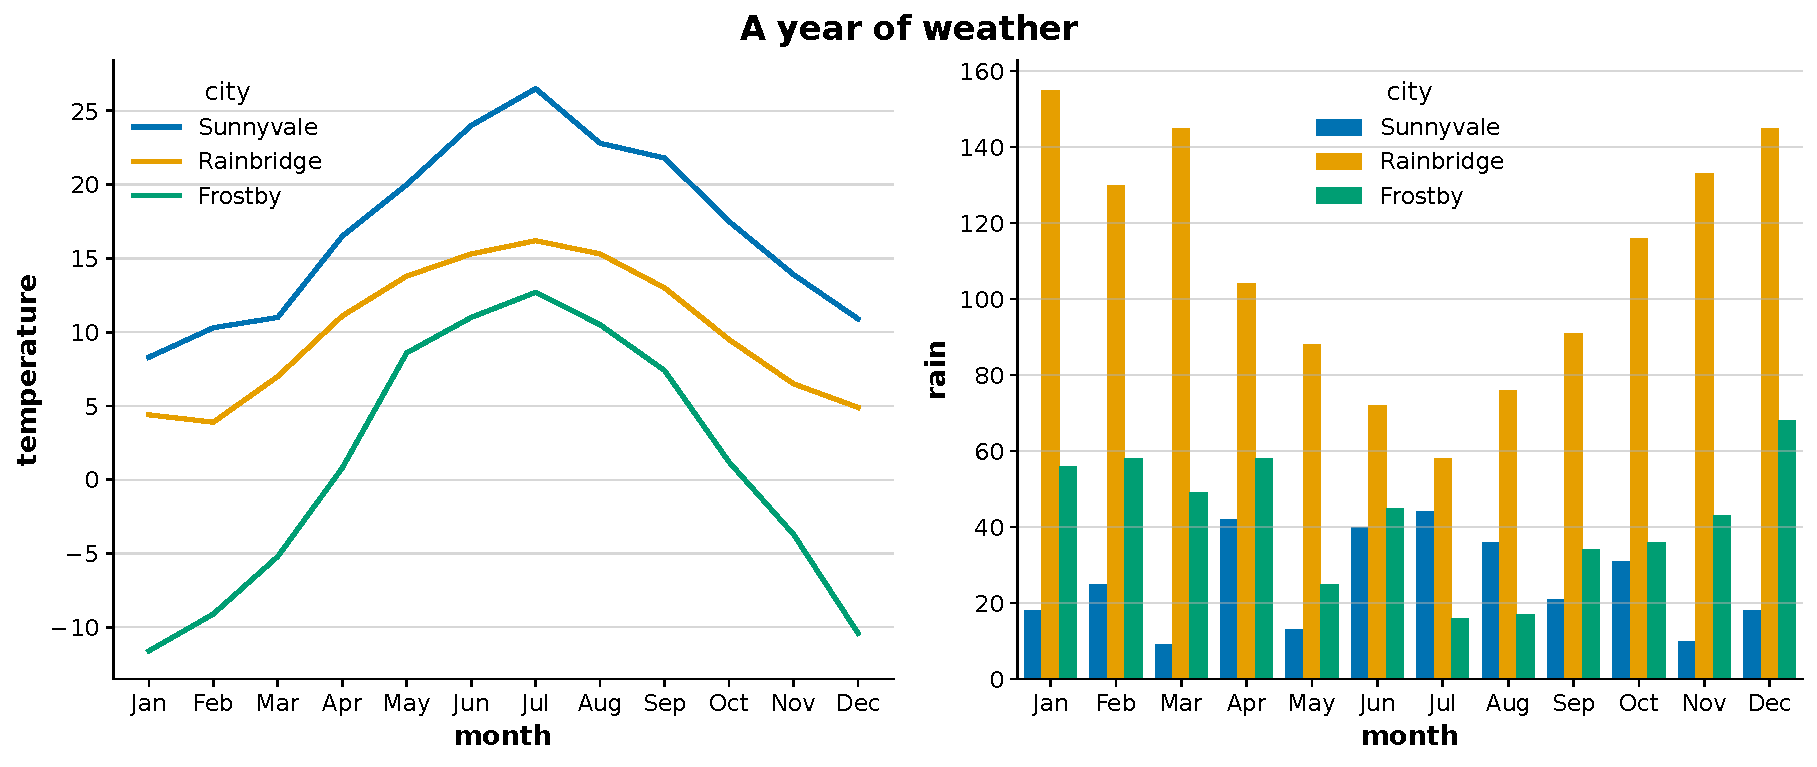
\includegraphics[width=0.52\textwidth,height=0.30\textheight,keepaspectratio]{figures/solution07_task2_lesson7_side_by_side.pdf}
\captionof*{figure}{Lesson 7, task 2: \code{lesson7\_\allowbreak{}side\_\allowbreak{}by\_\allowbreak{}side.\allowbreak{}png}.}
\end{minipage}\end{center}
\solutionanswer{The same two charts, now next to each other instead of one above the other.}
\solutiontask{3}{Make \code{sdata.\allowbreak{}draw\_\allowbreak{}all\_\allowbreak{}pairs} of \code{sdata.\allowbreak{}get\_\allowbreak{}example(\textquotedbl{}weather\textquotedbl{})} with \code{colour=\textquotedbl{}city\textquotedbl{}}.}
\begin{lstlisting}[style=py]
import simplydata as sdata
pairs = sdata.draw_all_pairs(sdata.get_example("weather"), colour="city")
pairs.save("lesson7_weather_pairs.png")
\end{lstlisting}
\printedoutput{output/solution07_task3.txt}
\begin{center}\begin{minipage}{\linewidth}\centering
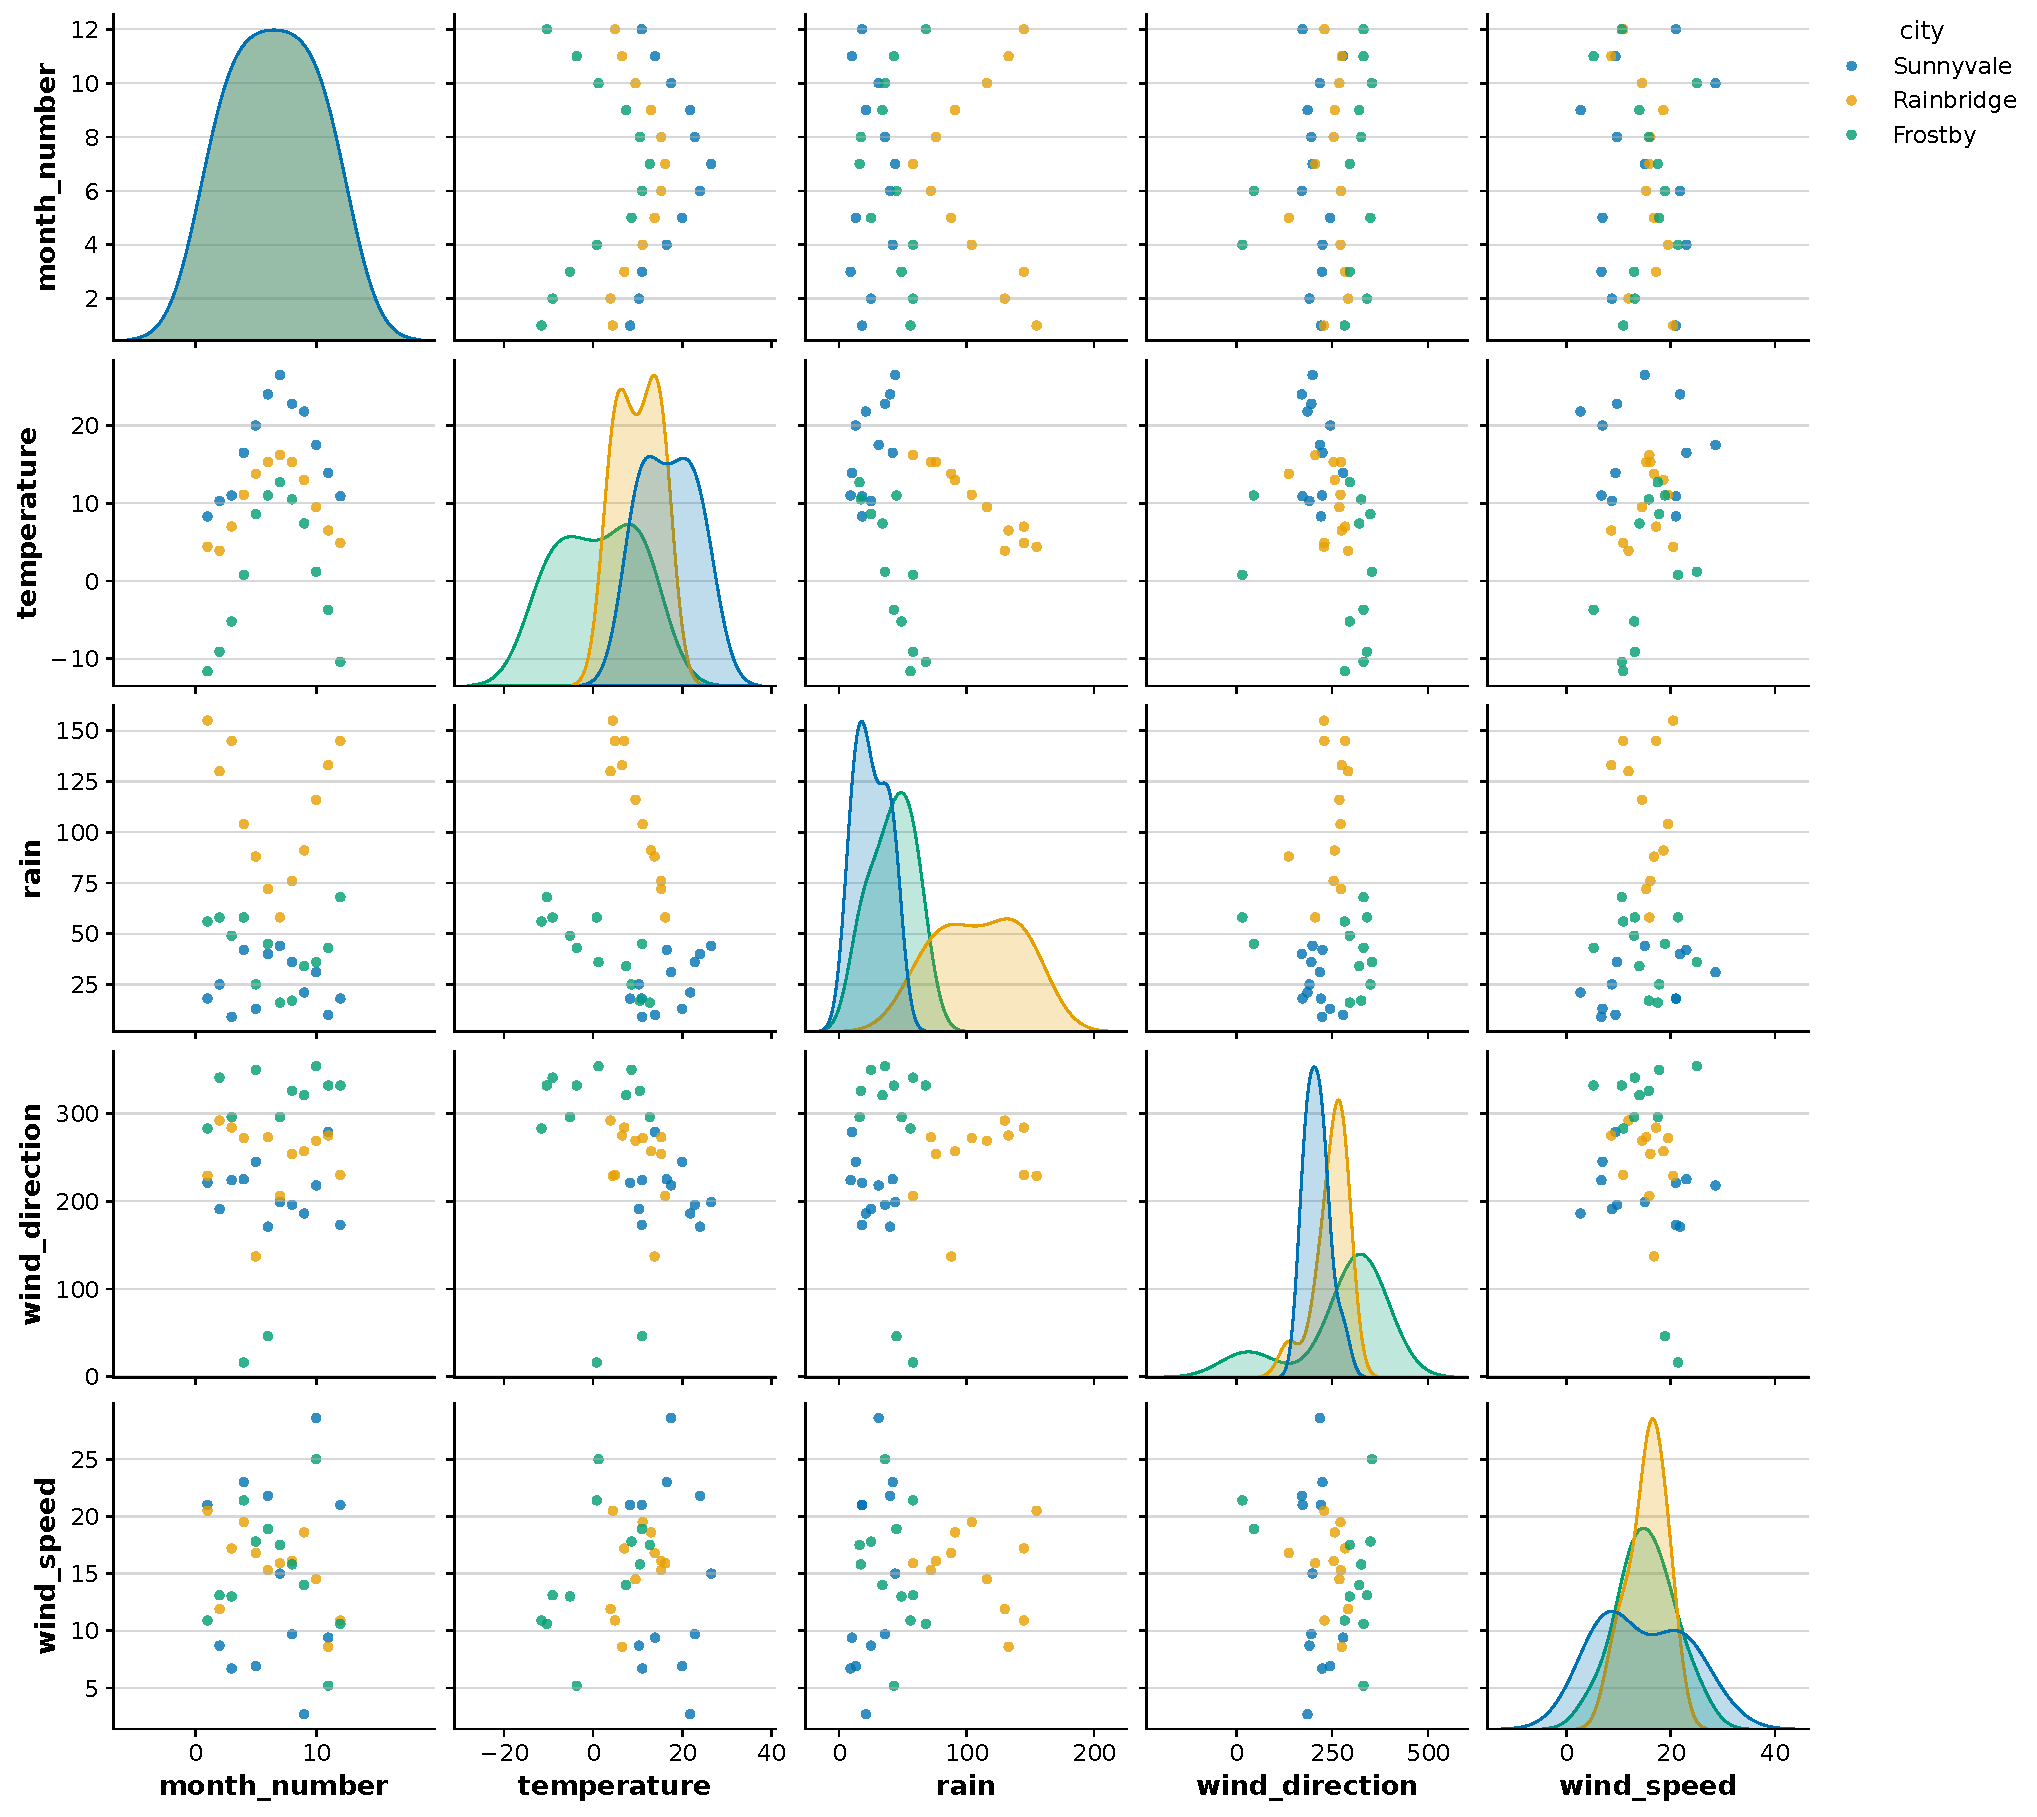
\includegraphics[width=0.52\textwidth,height=0.30\textheight,keepaspectratio]{figures/solution07_task3_lesson7_weather_pairs.pdf}
\captionof*{figure}{Lesson 7, task 3: \code{lesson7\_\allowbreak{}weather\_\allowbreak{}pairs.\allowbreak{}png}.}
\end{minipage}\end{center}
\solutionanswer{Every number column of the weather table against every other, one colour per city.}
\par\noindent{\small\sffamily\hyperref[lesson:7]{Back to lesson 7}}
\unsection{Lesson 8: Hard tricks, and your own program}{solutions:8}
\solutiontask{1}{Write your own program, from an empty file, for a question you care about.}
\begin{lstlisting}[style=py]
import simplydata as sdata
fruit = sdata.get_example("fruit")
print(fruit)
chart = sdata.chart(fruit)
chart.draw_bars(x="fruit", y="count", show="total")
chart.write_numbers_on_bars()
chart.write_title_on_top("Which fruit sells best?")
chart.label_x("Fruit")
chart.label_y("Sold in one week")
chart.save("lesson8_fruit.png")
\end{lstlisting}
\printedoutput{output/solution08_task1.txt}
\begin{center}\begin{minipage}{\linewidth}\centering
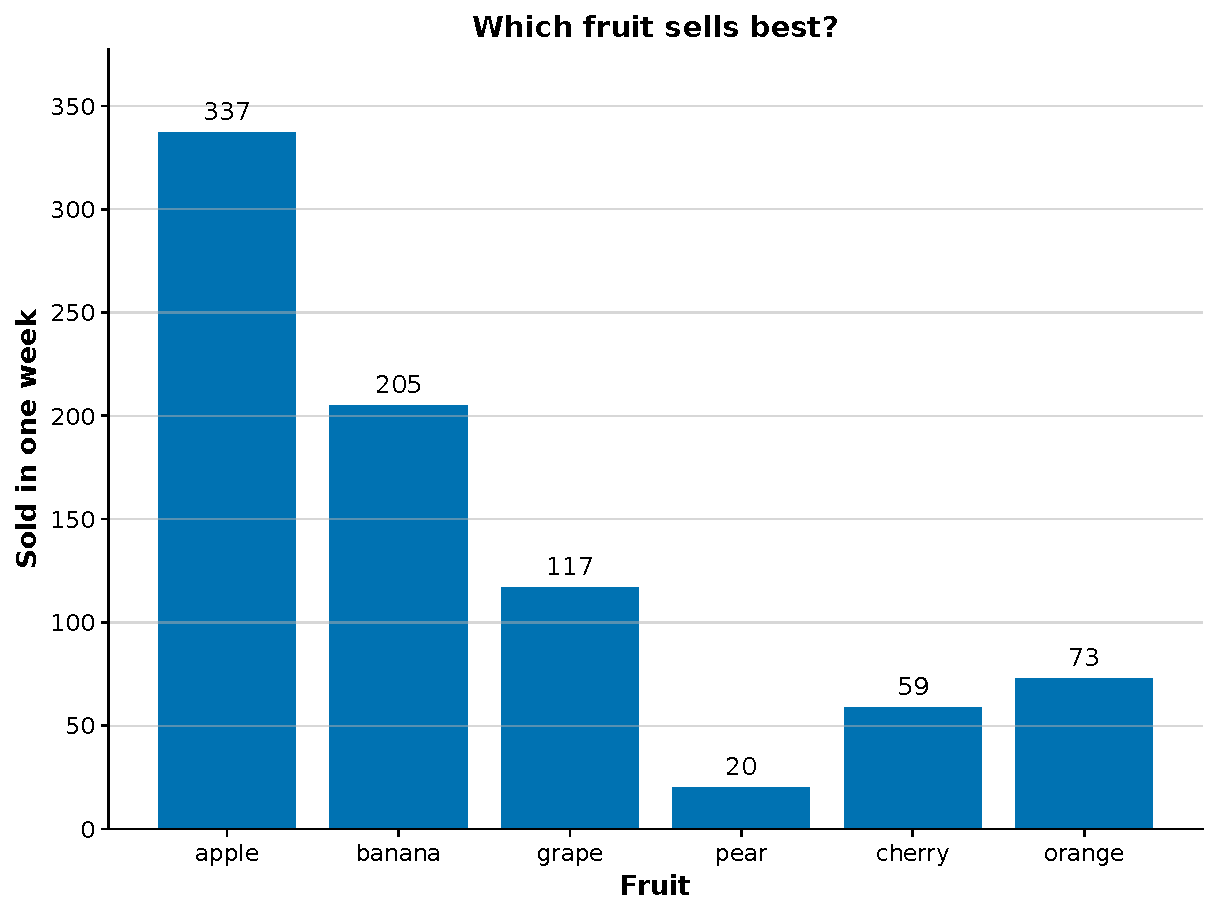
\includegraphics[width=0.52\textwidth,height=0.30\textheight,keepaspectratio]{figures/solution08_task1_lesson8_fruit.pdf}
\captionof*{figure}{Lesson 8, task 1: \code{lesson8\_\allowbreak{}fruit.\allowbreak{}png}.}
\end{minipage}\end{center}
\solutionanswer{One possible question: which fruit sells best? Same plan as always: get the data, look, start, draw, words, save.}
\solutiontask{2}{Use any example table, or your own. Give it a title, axis names and a note.}
\begin{lstlisting}[style=py]
import simplydata as sdata
growth = sdata.get_example("growth")
chart = sdata.chart(growth)
chart.draw_lines(x="year", y="forest", colour="country")
chart.write_title_on_top("Forest in four countries")
chart.label_x("Year")
chart.label_y("Forest (% of the land)")
chart.write_note("Applia loses the most", x=2016, y=50, with_arrow=True)
chart.save("lesson8_forest.png")
\end{lstlisting}
\printedoutput{output/solution08_task2.txt}
\begin{center}\begin{minipage}{\linewidth}\centering
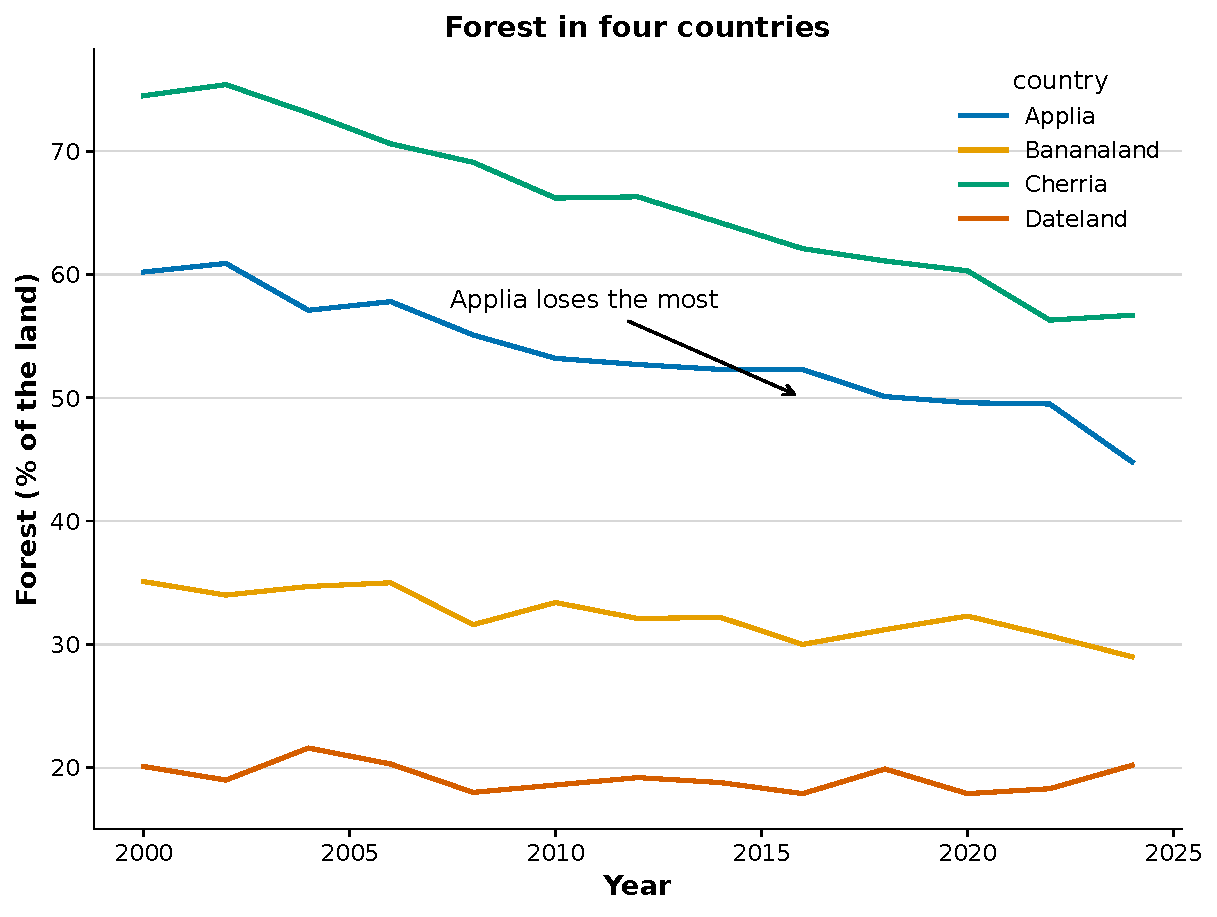
\includegraphics[width=0.52\textwidth,height=0.30\textheight,keepaspectratio]{figures/solution08_task2_lesson8_forest.pdf}
\captionof*{figure}{Lesson 8, task 2: \code{lesson8\_\allowbreak{}forest.\allowbreak{}png}.}
\end{minipage}\end{center}
\solutionanswer{Another table, with a title, both axis names and a note with an arrow.}
\solutiontask{3}{Make a second chart of the same table, put the two charts side by side and save the page as a PDF.}
\begin{lstlisting}[style=py]
import simplydata as sdata
growth = sdata.get_example("growth")
people = sdata.chart(growth).draw_lines(x="year", y="population", colour="country")
people.label_y("People (millions)")
forest = sdata.chart(growth).draw_lines(x="year", y="forest", colour="country")
forest.label_y("Forest (% of the land)")
page = sdata.put_side_by_side(people, forest, with_letters=True)
page.save("lesson8_page.pdf")
\end{lstlisting}
\printedoutput{output/solution08_task3.txt}
\begin{center}\begin{minipage}{\linewidth}\centering
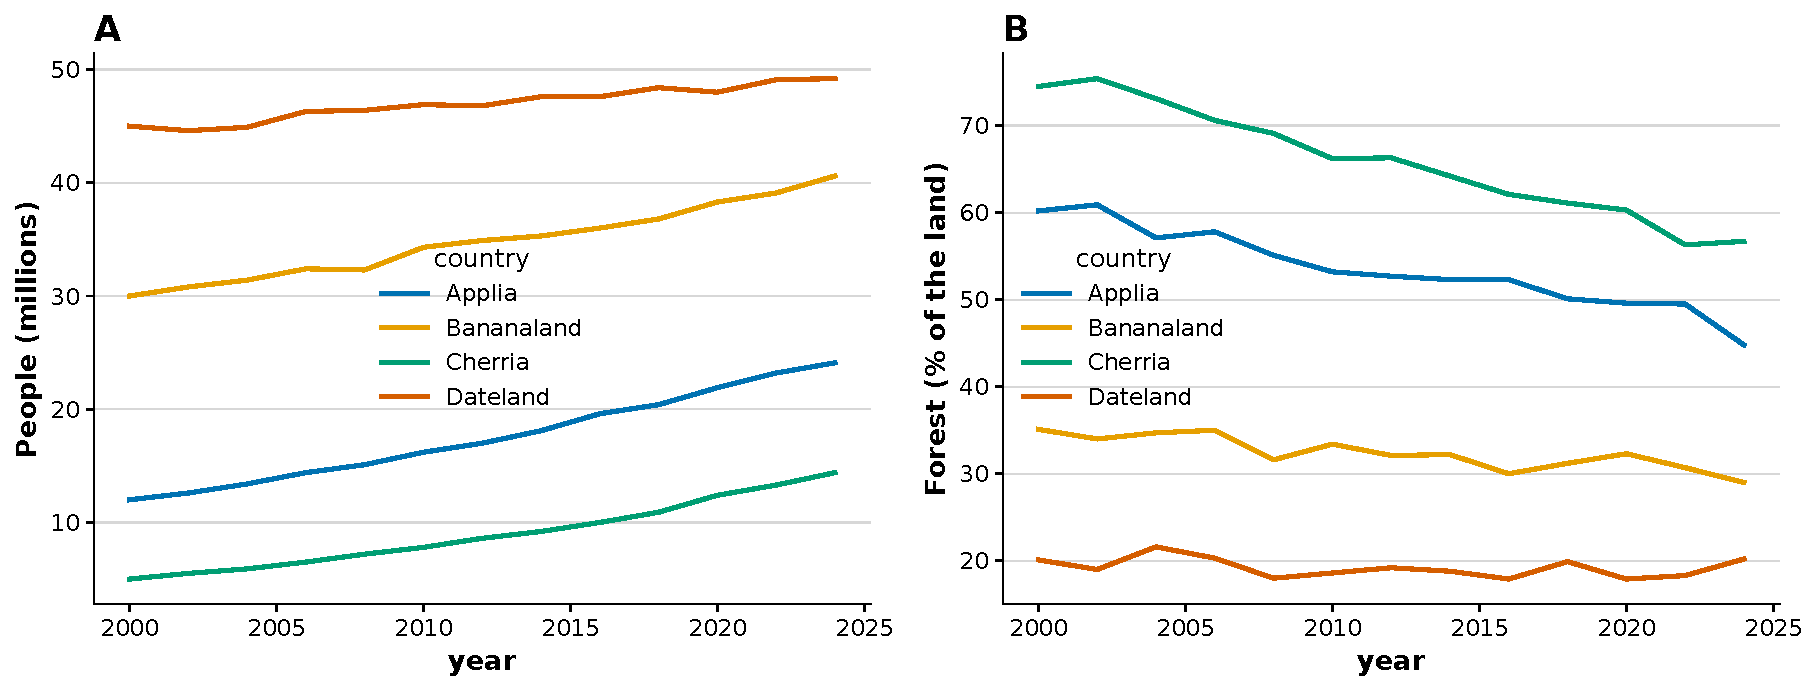
\includegraphics[width=0.52\textwidth,height=0.30\textheight,keepaspectratio]{figures/solution08_task3_lesson8_page.pdf}
\captionof*{figure}{Lesson 8, task 3: \code{lesson8\_\allowbreak{}page.\allowbreak{}pdf}.}
\end{minipage}\end{center}
\solutionanswer{Two charts of one table on one page, saved as a PDF because the name ends in \code{.\allowbreak{}pdf}.}
\par\noindent{\small\sffamily\hyperref[lesson:8]{Back to lesson 8}}
\unsection{Lesson 9: Tables: open one and look at it}{solutions:9}
\solutiontask{1}{Make a table of \code{sdata.\allowbreak{}get\_\allowbreak{}example(\textquotedbl{}weather\textquotedbl{})}. How many rows does it have?}
\begin{lstlisting}[style=py]
import simplydata as sdata
table = sdata.table(sdata.get_example("weather"))
table.count_rows()
\end{lstlisting}
\printedoutput{output/solution09_task1.txt}
\solutionanswer{36 rows: 12 months for each of 3 cities.}
\solutiontask{2}{Describe its columns. Which column has the biggest numbers?}
\begin{lstlisting}[style=py]
import simplydata as sdata
table = sdata.table(sdata.get_example("weather"))
table.describe_columns()
\end{lstlisting}
\printedoutput{output/solution09_task2.txt}
\solutionanswer{\code{wind\_\allowbreak{}direction} has the biggest numbers (up to 354): it is an angle in degrees, from 0 to 360.}
\solutiontask{3}{Count each \code{\textquotedbl{}city\textquotedbl{}}. Does every city have the same number of rows?}
\begin{lstlisting}[style=py]
import simplydata as sdata
table = sdata.table(sdata.get_example("weather"))
table.count_each("city")
\end{lstlisting}
\printedoutput{output/solution09_task3.txt}
\solutionanswer{Yes: Frostby, Rainbridge and Sunnyvale have 12 rows each, one for every month.}
\par\noindent{\small\sffamily\hyperref[lesson:9]{Back to lesson 9}}
\unsection{Lesson 10: Tables: choose rows and columns, and undo}{solutions:10}
\solutiontask{1}{In the marks table, keep only class \code{\textquotedbl{}B\textquotedbl{}} and sort by \code{\textquotedbl{}hours\textquotedbl{}}. Who studied the longest?}
\begin{lstlisting}[style=py]
import simplydata as sdata
table = sdata.table(sdata.get_example("marks"))
table.keep_rows_where("class", is_equal_to="B")
table.sort_by("hours", biggest_first=True)
table.show_first_rows(3)
\end{lstlisting}
\printedoutput{output/solution10_task1.txt}
\solutionanswer{Jade studied the longest: 9.4 hours, for Maths. \code{biggest\_\allowbreak{}first=True} puts the longest on top.}
\solutiontask{2}{Undo the sorting, then sort by name instead.}
\begin{lstlisting}[style=py]
import simplydata as sdata
table = sdata.table(sdata.get_example("marks"))
table.keep_rows_where("class", is_equal_to="B")
table.sort_by("hours", biggest_first=True)
table.undo()
table.sort_by("name")
table.show_first_rows()
\end{lstlisting}
\printedoutput{output/solution10_task2.txt}
\solutionanswer{\code{undo()} takes back only the sorting; class B stays. Text is sorted from A to Z.}
\solutiontask{3}{Keep 5 random rows with \code{table.\allowbreak{}keep\_\allowbreak{}random\_\allowbreak{}rows(5,\allowbreak{} with\_\allowbreak{}seed=1)} and save them as \code{\textquotedbl{}five.\allowbreak{}csv\textquotedbl{}}.}
\begin{lstlisting}[style=py]
import simplydata as sdata
table = sdata.table(sdata.get_example("marks"))
table.keep_random_rows(5, with_seed=1)
print(table)
table.save("five.csv")
\end{lstlisting}
\printedoutput{output/solution10_task3.txt}
\solutionanswer{\code{with\_\allowbreak{}seed=1} picks the same 5 rows every time, so someone else can repeat it.}
\solutiontask{4}{With one written condition, keep the rows with marks below 50 or hours above 8. How many rows are there?}
\begin{lstlisting}[style=py]
import simplydata as sdata
table = sdata.table(sdata.get_example("marks"))
table.keep_rows_where("marks < 50 or hours > 8")
table.count_rows()
\end{lstlisting}
\printedoutput{output/solution10_task4.txt}
\solutionanswer{19 rows: or keeps a row when at least one of the two is true.}
\solutiontask{5}{From memory, without looking back: start again, keep rows 5 to 9, then remove the last row. How many rows are left, and whose name is in row 1 now?}
\begin{lstlisting}[style=py]
import simplydata as sdata
table = sdata.table(sdata.get_example("marks"))
table.keep_rows_by_position(5, to=9)
table.remove_rows_by_position("last")
table.count_rows()
print(table.get_cell_at(row=1, column="name"))
\end{lstlisting}
\printedoutput{output/solution10_task5.txt}
\solutionanswer{4 rows: rows 5 to 9 are 5 rows (both ends count), and one is removed. Row 1 is now Ben's Science mark, which was row 5 before: positions are always of the table as it is now.}
\par\noindent{\small\sffamily\hyperref[lesson:10]{Back to lesson 10}}
\unsection{Lesson 11: Tables: clean the data and add new columns}{solutions:11}
\solutiontask{1}{In the first example, fill the empty marks with the median instead of the average.}
\begin{lstlisting}[style=py]
import simplydata as sdata
table = sdata.table(sdata.get_example("marks"))
table.replace_values_in("marks", [61, 73], with_value=None)
table.count_empty_cells_in()
table.fill_empty_cells_in("marks", with_the="median")
table.count_empty_cells_in()
\end{lstlisting}
\printedoutput{output/solution11_task1.txt}
\solutionanswer{\code{with\_\allowbreak{}the=\textquotedbl{}median\textquotedbl{}} fills each empty mark with the middle mark of the others; afterwards no cell is empty.}
\solutiontask{2}{Add a column \code{\textquotedbl{}height\_\allowbreak{}m\textquotedbl{}} with the height in metres: \code{from\_\allowbreak{}column=\textquotedbl{}height\textquotedbl{}}, \code{divide\_\allowbreak{}by=100}.}
\begin{lstlisting}[style=py]
import simplydata as sdata
table = sdata.table(sdata.get_example("marks"))
table.add_column("height_m", from_column="height", divide_by=100)
table.show_first_rows()
\end{lstlisting}
\printedoutput{output/solution11_task2.txt}
\solutionanswer{The height in centimetres divided by 100: 144 becomes 1.44.}
\solutiontask{3}{In the last example, add a column \code{\textquotedbl{}best\_\allowbreak{}two\textquotedbl{}} with the formula \code{\textquotedbl{}total - English\textquotedbl{}}.}
\begin{lstlisting}[style=py]
import simplydata as sdata
table = sdata.table(sdata.get_example("marks"))
table.keep_columns("name", "class", "subject", "marks")
table.turn_rows_into_columns(names_from="subject", values_from="marks")
table.add_column("total", "Maths + Science + English")
table.add_column("best_two", "total - English")
table.show_first_rows()
\end{lstlisting}
\printedoutput{output/solution11_task3.txt}
\solutionanswer{The formula can use a column made earlier (total); \code{best\_\allowbreak{}two} is Maths + Science.}
\solutiontask{4}{In the shop example, add a column \code{\textquotedbl{}change\textquotedbl{}} with the change in sales from the day before, \code{for\_\allowbreak{}each\_\allowbreak{}group\_\allowbreak{}in=\textquotedbl{}shop\textquotedbl{}} and \code{sorted\_\allowbreak{}by=\textquotedbl{}date\textquotedbl{}} (\code{add\_\allowbreak{}change\_\allowbreak{}column}).}
\begin{lstlisting}[style=py]
import simplydata as sdata
table = sdata.table(sdata.get_example("shop"))
table.fill_empty_cells_in("sales", with_the="line between neighbours", sorted_by="date", for_each_group_in="shop")
table.add_change_column("change", from_column="sales", for_each_group_in="shop", sorted_by="date")
table.show(rows=5)
\end{lstlisting}
\printedoutput{output/solution11_task4.txt}
\solutionanswer{Each change is today's sales minus yesterday's, in the same shop; the first day of each shop has nothing before it, so its change is empty.}
\par\noindent{\small\sffamily\hyperref[lesson:11]{Back to lesson 11}}
\unsection{Lesson 12: Tables: summaries, and from a table to a chart}{solutions:12}
\solutiontask{1}{Make the fruit totals \code{for\_\allowbreak{}each\_\allowbreak{}group\_\allowbreak{}in=\textquotedbl{}shop\textquotedbl{}} instead. Which shop sold more?}
\begin{lstlisting}[style=py]
import simplydata as sdata
table = sdata.table(sdata.get_example("fruit"))
totals = table.find_total_of("count", for_each_group_in="shop")
print(totals)
\end{lstlisting}
\printedoutput{output/solution12_task1.txt}
\solutionanswer{The Market stall sold more: 457 pieces of fruit, against 354 at the Corner shop.}
\solutiontask{2}{Work out the average temperature \code{for\_\allowbreak{}each\_\allowbreak{}group\_\allowbreak{}in=\textquotedbl{}city\textquotedbl{}} in the weather table and draw it as bars.}
\begin{lstlisting}[style=py]
import simplydata as sdata
table = sdata.table(sdata.get_example("weather"))
averages = table.find_average_of("temperature", for_each_group_in="city")
chart = averages.start_chart()
chart.draw_bars(x="city", y="average of temperature")
chart.write_numbers_on_bars(with_decimals=1)
chart.save("lesson12_temperature.png")
\end{lstlisting}
\printedoutput{output/solution12_task2.txt}
\begin{center}\begin{minipage}{\linewidth}\centering
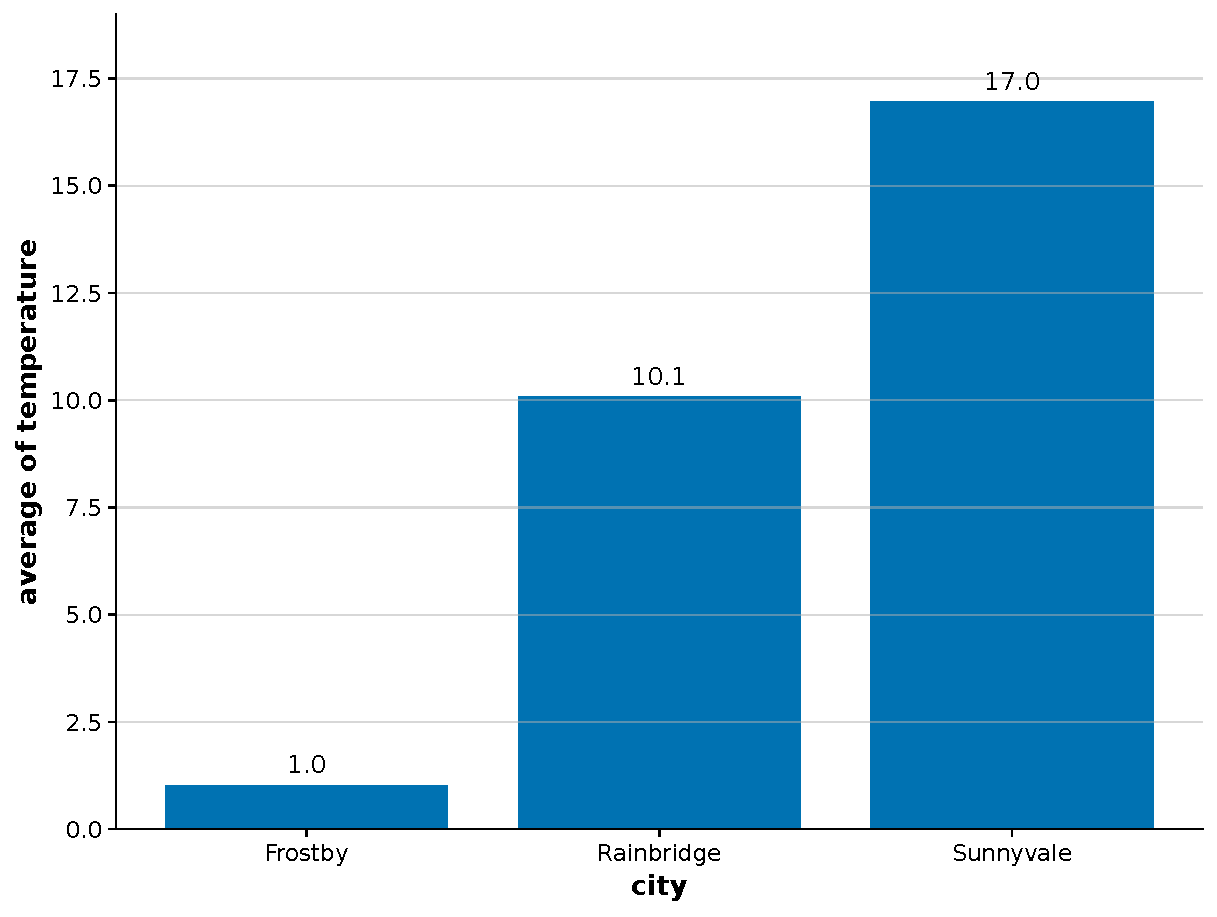
\includegraphics[width=0.52\textwidth,height=0.30\textheight,keepaspectratio]{figures/solution12_task2_lesson12_temperature.pdf}
\captionof*{figure}{Lesson 12, task 2: \code{lesson12\_\allowbreak{}temperature.\allowbreak{}png}.}
\end{minipage}\end{center}
\solutionanswer{Frostby 1.0, Rainbridge 10.1 and Sunnyvale 17.0 degrees. The summary table's column is called \code{\textquotedbl{}average of temperature\textquotedbl{}}.}
\solutiontask{3}{Is there a link between height and marks? Use \code{find\_\allowbreak{}correlation\_\allowbreak{}between} to find out.}
\begin{lstlisting}[style=py]
import simplydata as sdata
table = sdata.table(sdata.get_example("marks"))
table.find_correlation_between("height", "marks")
\end{lstlisting}
\printedoutput{output/solution12_task3.txt}
\solutionanswer{No: r = 0.03, very close to 0. Even with truly no link, a link this strong would turn up in about 83 of 100 studies (p = 0.83).}
\solutiontask{4}{Make a cross table of the average mark \code{for\_\allowbreak{}each\_\allowbreak{}group\_\allowbreak{}in=\textquotedbl{}subject\textquotedbl{}} \code{across=\textquotedbl{}class\textquotedbl{}}. Which class is best in Science?}
\begin{lstlisting}[style=py]
import simplydata as sdata
table = sdata.table(sdata.get_example("marks"))
table.find_average_of("marks", for_each_group_in="subject", across="class")
\end{lstlisting}
\printedoutput{output/solution12_task4.txt}
\solutionanswer{Class A, with an average of 79.2 in Science, against 67.5 for B and 62.3 for C.}
\par\noindent{\small\sffamily\hyperref[lesson:12]{Back to lesson 12}}
\unsection{Lesson 13: Numbers: lists and grids of numbers}{solutions:13}
\solutiontask{1}{Make the numbers 1 to 10, then square them in two ways: with ** 2 and with \code{raise\_\allowbreak{}to\_\allowbreak{}power(2)}.}
\begin{lstlisting}[style=py]
import simplydata as sdata
nums = sdata.numbers(1, to=10)
squares = nums ** 2
print(squares)
nums.raise_to_power(2)
nums.show()
\end{lstlisting}
\printedoutput{output/solution13_task1.txt}
\solutionanswer{Both give 1, 4, 9 ... 100. ** 2 makes new numbers and leaves nums alone; \code{raise\_\allowbreak{}to\_\allowbreak{}power(2)} changes nums itself (and \code{undo()} can take it back).}
\solutiontask{2}{Make 6 dice throws with \code{sdata.\allowbreak{}make\_\allowbreak{}random\_\allowbreak{}numbers(how\_\allowbreak{}many=6,\allowbreak{} between=[1,\allowbreak{} 6],\allowbreak{} whole\_\allowbreak{}numbers=True,\allowbreak{} with\_\allowbreak{}seed=1)}. What is their total?}
\begin{lstlisting}[style=py]
import simplydata as sdata
dice = sdata.make_random_numbers(how_many=6, between=[1, 6], whole_numbers=True, with_seed=1)
dice.show()
dice.find_total()
\end{lstlisting}
\printedoutput{output/solution13_task2.txt}
\solutionanswer{With \code{with\_\allowbreak{}seed=1} the throws are 3, 4, 5, 6, 1 and 1, which add up to 20.}
\solutiontask{3}{Make a grid of 3 rows and 4 columns filled with 0: \code{sdata.\allowbreak{}number\_\allowbreak{}grid(rows=3,\allowbreak{} columns=4,\allowbreak{} filled\_\allowbreak{}with=0)}.}
\begin{lstlisting}[style=py]
import simplydata as sdata
grid = sdata.number_grid(rows=3, columns=4, filled_with=0)
print(grid)
\end{lstlisting}
\printedoutput{output/solution13_task3.txt}
\solutionanswer{Three rows of four zeros: a grid to fill in later.}
\par\noindent{\small\sffamily\hyperref[lesson:13]{Back to lesson 13}}
\unsection{Lesson 14: Statistical tests: real difference, or chance?}{solutions:14}
\solutiontask{1}{Compare the average marks \code{for\_\allowbreak{}each\_\allowbreak{}group\_\allowbreak{}in=\textquotedbl{}subject\textquotedbl{}}. Could the differences be chance?}
\begin{lstlisting}[style=py]
import simplydata as sdata
table = sdata.table(sdata.get_example("marks"))
table.compare_averages_of("marks", for_each_group_in="subject")
\end{lstlisting}
\printedoutput{output/solution14_task1.txt}
\solutionanswer{Yes, they could: p = 0.26 is well above 0.05. That does not prove the subjects are the same; these data simply cannot tell.}
\solutiontask{2}{Is the average temperature different between the cities of \code{sdata.\allowbreak{}get\_\allowbreak{}example(\textquotedbl{}weather\textquotedbl{})}?}
\begin{lstlisting}[style=py]
import simplydata as sdata
table = sdata.table(sdata.get_example("weather"))
table.compare_averages_of("temperature", for_each_group_in="city")
table.compare_each_pair_of("temperature", for_each_group_in="city")
\end{lstlisting}
\printedoutput{output/solution14_task2.txt}
\solutionanswer{Yes: if the cities truly had the same average, differences this big would turn up in fewer than 1 in 1000 studies (p = 0.0002). \code{compare\_\allowbreak{}each\_\allowbreak{}pair\_\allowbreak{}of} then shows which cities differ from each other.}
\solutiontask{3}{Fit a straight line of \code{\textquotedbl{}forest\textquotedbl{}} against \code{\textquotedbl{}year\textquotedbl{}} in \code{sdata.\allowbreak{}get\_\allowbreak{}example(\textquotedbl{}growth\textquotedbl{})} for one country.}
\begin{lstlisting}[style=py]
import simplydata as sdata
table = sdata.table(sdata.get_example("growth"))
table.keep_rows_where("country", is_equal_to="Applia")
table.fit_line(x="year", y="forest")
\end{lstlisting}
\printedoutput{output/solution14_task3.txt}
\solutionanswer{In Applia the forest shrinks by about 0.57 percentage points a year (95 \% CI 0.48 to 0.67), and the line explains 94 \% of the differences.}
\solutiontask{4}{Remove the rows with outliers in \code{\textquotedbl{}marks\textquotedbl{}} \code{for\_\allowbreak{}each\_\allowbreak{}group\_\allowbreak{}in=\textquotedbl{}class\textquotedbl{}}, then compare the average marks \code{for\_\allowbreak{}each\_\allowbreak{}group\_\allowbreak{}in=\textquotedbl{}class\textquotedbl{}} again. Did the answer change?}
\begin{lstlisting}[style=py]
import simplydata as sdata
table = sdata.table(sdata.get_example("marks"))
table.remove_rows_with_outliers("marks", for_each_group_in="class")
table.compare_averages_of("marks", for_each_group_in="class")
\end{lstlisting}
\printedoutput{output/solution14_task4.txt}
\solutionanswer{Only one mark (33 in class B) is removed. Class B goes up from 64.3 to 66.1, but p stays 0.028: the answer does not change. Say in a report that you checked, and how.}
\par\noindent{\small\sffamily\hyperref[lesson:14]{Back to lesson 14}}
\unsection{Lesson 15: A whole analysis: from a question to a figure}{solutions:15}
\solutiontask{1}{Do a whole analysis of \code{sdata.\allowbreak{}get\_\allowbreak{}example(\textquotedbl{}weather\textquotedbl{})}: look at it, compare the average rain \code{for\_\allowbreak{}each\_\allowbreak{}group\_\allowbreak{}in=\textquotedbl{}city\textquotedbl{}}, draw the rain of each city as boxes, and save the chart and the table.}
\begin{lstlisting}[style=py]
import simplydata as sdata
table = sdata.table(sdata.get_example("weather"))
table.describe_columns()
table.remove_columns("wind_direction", "wind_speed")
table.find_average_of("rain", for_each_group_in="city")
table.compare_averages_of("rain", for_each_group_in="city")
chart = table.start_chart()
chart.draw_boxes(x="city", y="rain")
chart.draw_all_dots(x="city", y="rain")
chart.label_y("Rain (mm)")
chart.save("lesson15_rain_boxes.png")
table.save("lesson15_weather.xlsx")
\end{lstlisting}
\printedoutput{output/solution15_task1.txt}
\begin{center}\begin{minipage}{\linewidth}\centering
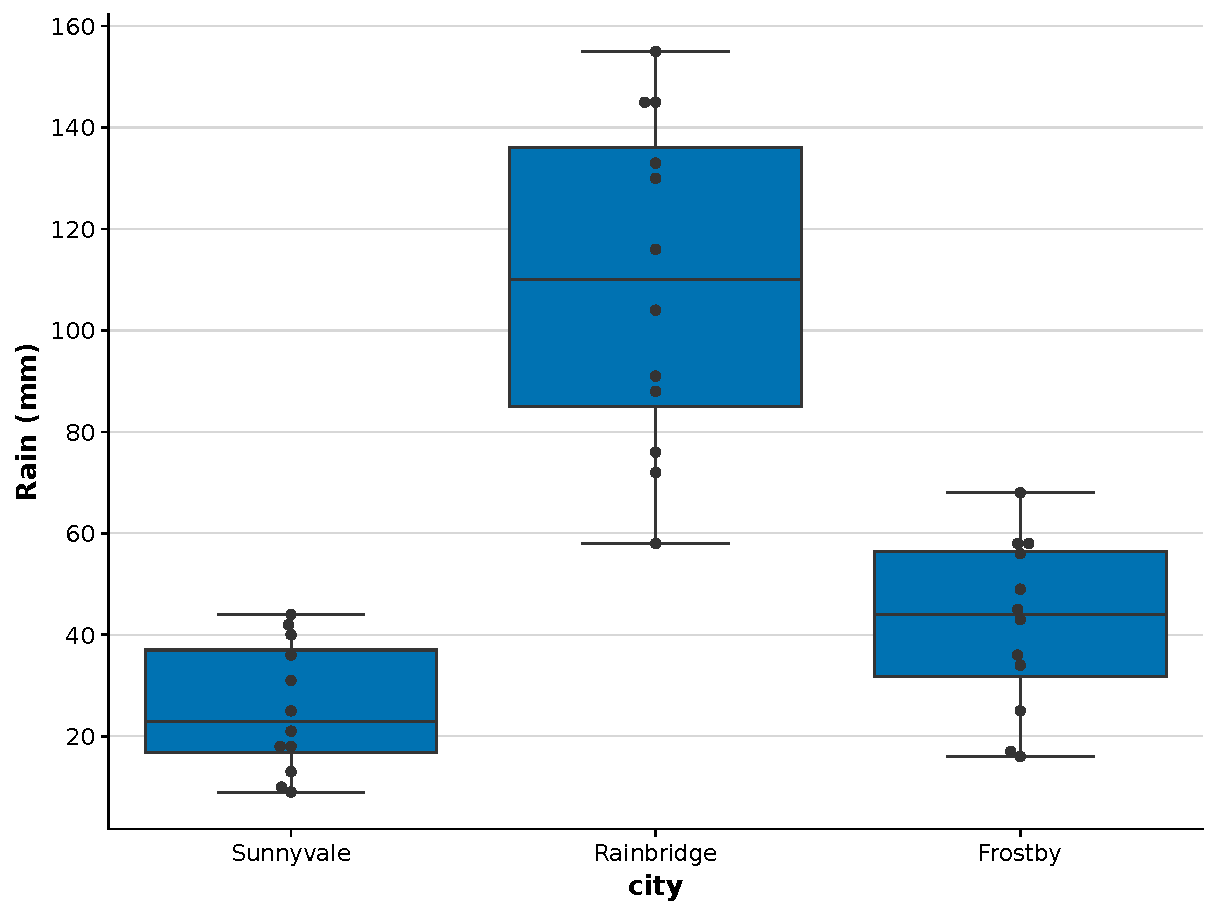
\includegraphics[width=0.52\textwidth,height=0.30\textheight,keepaspectratio]{figures/solution15_task1_lesson15_rain_boxes.pdf}
\captionof*{figure}{Lesson 15, task 1: \code{lesson15\_\allowbreak{}rain\_\allowbreak{}boxes.\allowbreak{}png}.}
\end{minipage}\end{center}
\solutionanswer{Rainbridge is much wetter (109 mm a month on average) than Frostby (42) and Sunnyvale (26); if the cities truly had the same rain, differences this big would turn up in fewer than 1 in 1000 studies (p \textless{} 0.0001).}
\solutiontask{2}{Make a second chart of the temperature, then put the two charts together with \code{sdata.\allowbreak{}put\_\allowbreak{}side\_\allowbreak{}by\_\allowbreak{}side(.\allowbreak{}.\allowbreak{}.\allowbreak{},\allowbreak{} with\_\allowbreak{}letters=True)}.}
\begin{lstlisting}[style=py]
import simplydata as sdata
table = sdata.table(sdata.get_example("weather"))
rain = table.start_chart()
rain.draw_boxes(x="city", y="rain")
rain.label_y("Rain (mm)")
warmth = table.start_chart()
warmth.draw_lines(x="month", y="temperature", colour="city")
warmth.label_y("Temperature (°C)")
page = sdata.put_side_by_side(rain, warmth, with_letters=True)
page.save("lesson15_weather_page.png")
\end{lstlisting}
\printedoutput{output/solution15_task2.txt}
\begin{center}\begin{minipage}{\linewidth}\centering
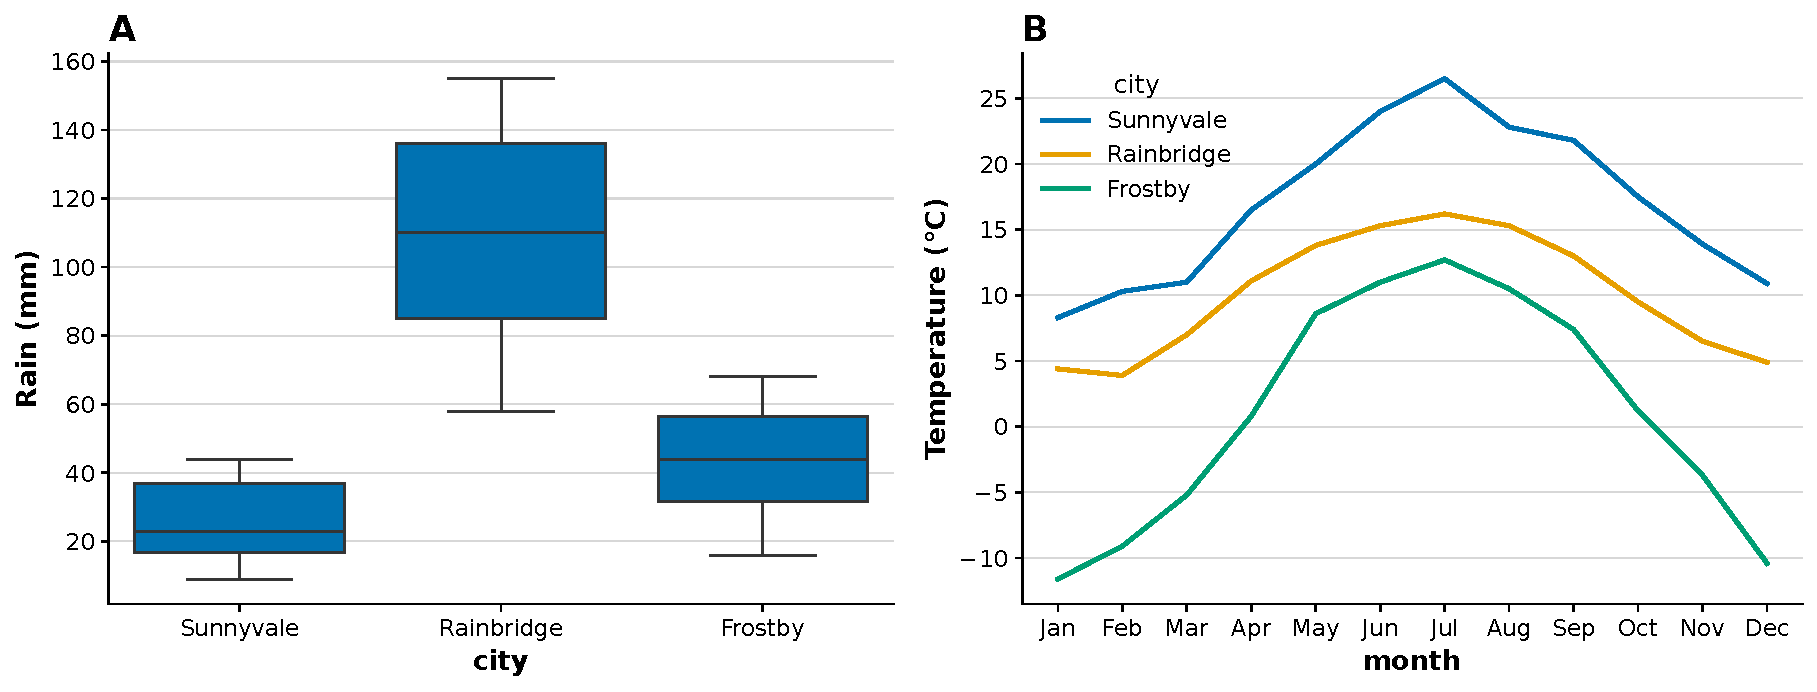
\includegraphics[width=0.52\textwidth,height=0.30\textheight,keepaspectratio]{figures/solution15_task2_lesson15_weather_page.pdf}
\captionof*{figure}{Lesson 15, task 2: \code{lesson15\_\allowbreak{}weather\_\allowbreak{}page.\allowbreak{}png}.}
\end{minipage}\end{center}
\solutionanswer{Two charts of one table, side by side, with A and B so a report can point to each.}
\solutiontask{3}{Read the \code{show\_\allowbreak{}steps()} of your table out loud. Would someone else understand what you did?}
\begin{lstlisting}[style=py]
import simplydata as sdata
table = sdata.table(sdata.get_example("weather"))
table.remove_columns("wind_direction", "wind_speed")
table.keep_rows_where("month_number", is_between=[6, 8])
table.sort_by("rain", biggest_first=True)
table.show_steps()
\end{lstlisting}
\printedoutput{output/solution15_task3.txt}
\solutionanswer{\code{show\_\allowbreak{}steps()} lists each change in plain words, in order; those lines are a first draft of the methods part of a report.}
\par\noindent{\small\sffamily\hyperref[lesson:15]{Back to lesson 15}}
\unsection{Lesson 16: Models: explain one column from several others}{solutions:16}
\solutiontask{1}{Explain \code{\textquotedbl{}marks\textquotedbl{}} using \code{\textquotedbl{}hours\textquotedbl{}} and \code{\textquotedbl{}school\textquotedbl{}} (school as a column of groups). Which schools differ from School A, and is school as a whole important?}
\begin{lstlisting}[style=py]
import simplydata as sdata
table = sdata.table(sdata.get_example("school"))
table.explain("marks", using=["hours", "school"])
\end{lstlisting}
\printedoutput{output/solution16_task1.txt}
\solutionanswer{School as a whole matters a lot (F = 10.4, p \textless{} 0.0001); School D scores about 15 marks more than School A for the same hours of study. \code{grouped\_\allowbreak{}by=} would instead treat the schools as a sample of many possible schools.}
\solutiontask{2}{Explain \code{\textquotedbl{}passed\textquotedbl{}} using \code{\textquotedbl{}hours\textquotedbl{}} and \code{\textquotedbl{}sleep\textquotedbl{}} with \code{outcome=\textquotedbl{}yes or no\textquotedbl{}}.}
\begin{lstlisting}[style=py]
import simplydata as sdata
table = sdata.table(sdata.get_example("school"))
table.explain("passed", using=["hours", "sleep"], outcome="yes or no")
\end{lstlisting}
\printedoutput{output/solution16_task2.txt}
\solutionanswer{Each extra hour of study multiplies the odds of passing by 1.69 and each extra hour of sleep by 1.98; with truly no effect, fewer than 1 in 1000 studies (hours) and about 2 of 1000 (sleep) would show this much.}
\solutiontask{3}{Explain \code{\textquotedbl{}days\_\allowbreak{}absent\textquotedbl{}} using \code{\textquotedbl{}hours\textquotedbl{}} and \code{\textquotedbl{}breakfast\textquotedbl{}} with \code{outcome=\textquotedbl{}counts\textquotedbl{}}. Does breakfast matter?}
\begin{lstlisting}[style=py]
import simplydata as sdata
table = sdata.table(sdata.get_example("school"))
table.explain("days_absent", using=["hours", "breakfast"], outcome="counts")
\end{lstlisting}
\printedoutput{output/solution16_task3.txt}
\solutionanswer{For breakfast the data cannot tell (rate ratio 0.94, p = 0.45: about 45 of 100 studies would show this much with truly no effect); study hours matter (rate ratio 0.86 for each hour).}
\solutiontask{4}{In the clinic table, explain \code{\textquotedbl{}caught\_\allowbreak{}infection\textquotedbl{}} using \code{\textquotedbl{}ward\textquotedbl{}} and \code{\textquotedbl{}patient\_\allowbreak{}days\textquotedbl{}} with \code{outcome=\textquotedbl{}yes or no\textquotedbl{}}, first as odds ratios and then with \code{show=\textquotedbl{}risk ratios\textquotedbl{}}. Which is further from 1?}
\begin{lstlisting}[style=py]
import simplydata as sdata
table = sdata.table(sdata.get_example("clinic"))
table.explain("caught_infection", using=["ward", "patient_days"], outcome="yes or no")
table.explain("caught_infection", using=["ward", "patient_days"], outcome="yes or no",
              show="risk ratios")
\end{lstlisting}
\printedoutput{output/solution16_task4.txt}
\solutionanswer{Ward B: odds ratio 5.80, risk ratio 4.63. The odds ratio is further from 1, even with only 1 patient in 10 infected; the rarer the outcome, the closer the two.}
\par\noindent{\small\sffamily\hyperref[lesson:16]{Back to lesson 16}}
\unsection{Lesson 17: Patterns across many columns}{solutions:17}
\solutiontask{1}{Add principal components of \code{\textquotedbl{}hours\textquotedbl{}}, \code{\textquotedbl{}sleep\textquotedbl{}}, \code{\textquotedbl{}marks\textquotedbl{}} and \code{\textquotedbl{}days\_\allowbreak{}absent\textquotedbl{}} in \code{sdata.\allowbreak{}get\_\allowbreak{}example(\textquotedbl{}school\textquotedbl{})}. Which columns weigh most in PC1?}
\begin{lstlisting}[style=py]
import simplydata as sdata
table = sdata.table(sdata.get_example("school"))
table.add_principal_components(columns=["hours", "sleep", "marks", "days_absent"])
\end{lstlisting}
\printedoutput{output/solution17_task1.txt}
\solutionanswer{PC1 (50 \% of the spread) is mostly hours, marks and, the other way, days absent: pupils who study more get better marks and miss fewer days. PC2 is mostly sleep.}
\solutiontask{2}{Make an NMDS map of the meadow in 3 dimensions. Is the stress lower than in 2?}
\begin{lstlisting}[style=py]
import simplydata as sdata
table = sdata.table(sdata.get_example("meadow"))
table.add_nmds(measure="bray-curtis", dimensions=3)
\end{lstlisting}
\printedoutput{output/solution17_task2.txt}
\solutionanswer{Yes: the stress drops from 0.195 to 0.127. That is still in the usable band (good is below 0.1), but the map keeps the distances clearly better.}
\solutiontask{3}{Do the three fields differ in make-up? Use \code{compare\_\allowbreak{}profiles\_\allowbreak{}of} with \code{for\_\allowbreak{}each\_\allowbreak{}group\_\allowbreak{}in=\textquotedbl{}field\textquotedbl{}}.}
\begin{lstlisting}[style=py]
import simplydata as sdata
table = sdata.table(sdata.get_example("meadow"))
table.compare_profiles_of(for_each_group_in="field")
\end{lstlisting}
\printedoutput{output/solution17_task3.txt}
\solutionanswer{The fields explain 12 \% of the differences, much less than grazing (25 \%); a difference this big would turn up in about 5 of 100 studies even if the fields had the same make-up (p = 0.053). The spread check finds no sign of a difference in spread (p = 0.53).}
\solutiontask{4}{Cluster the meadow plots with \code{method=\textquotedbl{}hierarchical\textquotedbl{}}. Do the clusters match the grazing?}
\begin{lstlisting}[style=py]
import simplydata as sdata
table = sdata.table(sdata.get_example("meadow"))
table.add_clusters(how_many=2, method="hierarchical")
table.count_rows(for_each_group_in="cluster", across="grazed")
\end{lstlisting}
\printedoutput{output/solution17_task4.txt}
\solutionanswer{Exactly: cluster 1 is the 15 grazed plots and cluster 2 the 15 ungrazed ones.}
\par\noindent{\small\sffamily\hyperref[lesson:17]{Back to lesson 17}}
\unsection{Lesson 18: Survival, and planning a study}{solutions:18}
\solutiontask{1}{Explain the risk of dying from \code{\textquotedbl{}age\textquotedbl{}} alone with \code{explain\_\allowbreak{}survival}.}
\begin{lstlisting}[style=py]
import simplydata as sdata
table = sdata.table(sdata.get_example("trial"))
table.explain_survival(time="days", event="died", using="age")
\end{lstlisting}
\printedoutput{output/solution18_task1.txt}
\solutionanswer{Each year of age multiplies the risk by 1.05 (95 \% CI 1.03 to 1.08), p \textless{} 0.0001.}
\solutiontask{2}{How many pairs does a before/after study need to find a small change (\code{effect\_\allowbreak{}size=0.\allowbreak{}3})?}
\begin{lstlisting}[style=py]
import simplydata as sdata
sdata.find_how_many_needed(test="compare_before_and_after", effect_size=0.3)
\end{lstlisting}
\printedoutput{output/solution18_task2.txt}
\solutionanswer{90 pairs, each with a before and an after value.}
\solutiontask{3}{What is the chance to find a medium difference (\code{effect\_\allowbreak{}size=0.\allowbreak{}25}) between 3 groups with 30 values in each?}
\begin{lstlisting}[style=py]
import simplydata as sdata
sdata.find_chance_of_finding(test="compare_averages", effect_size=0.25, groups=3, values_per_group=30)
\end{lstlisting}
\printedoutput{output/solution18_task3.txt}
\solutionanswer{Only 54 \%: too small. \code{find\_\allowbreak{}how\_\allowbreak{}many\_\allowbreak{}needed} with \code{groups=3} tells you how many to aim for.}
\par\noindent{\small\sffamily\hyperref[lesson:18]{Back to lesson 18}}
\unsection{Lesson 19: Fitting curves, finding the best value and solving}{solutions:19}
\solutiontask{1}{Fit a curve of degree 3 to \code{\textquotedbl{}marks\textquotedbl{}} against \code{\textquotedbl{}hours\textquotedbl{}}. Does R squared go up much from the straight line?}
\begin{lstlisting}[style=py]
import simplydata as sdata
table = sdata.table(sdata.get_example("marks"))
table.fit_curve(x="hours", y="marks", of_degree=3)
\end{lstlisting}
\printedoutput{output/solution19_task1.txt}
\solutionanswer{R squared is 0.71, against 0.69 for the straight line: the extra bends add very little.}
\solutiontask{2}{With the weather table, keep the city Sunnyvale and fit \code{\textquotedbl{}temperature = a + b * cos(2 * pi * (month\_\allowbreak{}number - c) / 12)\textquotedbl{}} with \code{start=}\{\code{\textquotedbl{}a\textquotedbl{}}: 15, \code{\textquotedbl{}b\textquotedbl{}}: 8, \code{\textquotedbl{}c\textquotedbl{}}: 7\}. In which month is it warmest (c)?}
\begin{lstlisting}[style=py]
import simplydata as sdata
table = sdata.table(sdata.get_example("weather"))
table.keep_rows_where("city", is_equal_to="Sunnyvale")
table.fit_formula("temperature = a + b * cos(2 * pi * (month_number - c) / 12)",
                  start={"a": 15, "b": 8, "c": 7})
\end{lstlisting}
\printedoutput{output/solution19_task2.txt}
\solutionanswer{c = 7.19: the warmest time is in July; a = 17.0 is the average and b = 8.18 how far it swings.}
\solutiontask{3}{Try to remember without looking back: which word finds where a formula is biggest, and which word finds where the two sides of an equation are equal? Use them on \code{\textquotedbl{}x * (10 - x)\textquotedbl{}} between 0 and 10, and on \code{\textquotedbl{}x**2 = 2\textquotedbl{}} between 0 and 2.}
\begin{lstlisting}[style=py]
import simplydata as sdata
sdata.find_where_biggest("x * (10 - x)", between=[0, 10])
sdata.solve("x**2 = 2", between=[0, 2])
\end{lstlisting}
\printedoutput{output/solution19_task3.txt}
\solutionanswer{\code{find\_\allowbreak{}biggest} gives 25 at x = 5, and solve gives x = 1.41421, the square root of 2.}
\par\noindent{\small\sffamily\hyperref[lesson:19]{Back to lesson 19}}
\unsection{Lesson 20: Distributions, chances and values between points}{solutions:20}
\solutiontask{1}{Ten coins are thrown. With \code{sdata.\allowbreak{}distribution(\textquotedbl{}binomial\textquotedbl{},\allowbreak{} tries=10,\allowbreak{} chance=0.\allowbreak{}5)}, what is the chance of 8 heads or more?}
\begin{lstlisting}[style=py]
import simplydata as sdata
coins = sdata.distribution("binomial", tries=10, chance=0.5)
coins.find_chance_that_value(is_at_least=8)
\end{lstlisting}
\printedoutput{output/solution20_task1.txt}
\solutionanswer{5.47 \%: 8, 9 or 10 heads happen about once in 18 tries.}
\solutiontask{2}{Which fits the daily \code{\textquotedbl{}sales\textquotedbl{}} of the shop table best: normal, lognormal, gamma or weibull? Then check the best one with \code{compare\_\allowbreak{}shape\_\allowbreak{}to}.}
\begin{lstlisting}[style=py]
import simplydata as sdata
table = sdata.table(sdata.get_example("shop"))
table.compare_distributions_for("sales")
table.compare_shape_to("sales", "lognormal")
\end{lstlisting}
\printedoutput{output/solution20_task2.txt}
\solutionanswer{Lognormal has the smallest AIC, and its shape could well fit (p = 0.65).}
\solutiontask{3}{Try to remember without looking back: which word estimates a value between the points you measured? Use it to estimate the temperature of each city at \code{month\_\allowbreak{}number} 6.5, joined by a smooth curve.}
\begin{lstlisting}[style=py]
import simplydata as sdata
table = sdata.table(sdata.get_example("weather"))
estimates = table.values_at("temperature", at={"month_number": [6.5]},
                            joined_by="smooth curve", for_each_group_in="city")
estimates.show()
\end{lstlisting}
\printedoutput{output/solution20_task3.txt}
\solutionanswer{\code{values\_\allowbreak{}at} joins the months with a smooth curve and reads off each city at 6.5.}
\par\noindent{\small\sffamily\hyperref[lesson:20]{Back to lesson 20}}
\unsection{Lesson 21: Working with a model: check it, compare it, predict with it}{solutions:21}
\solutiontask{1}{Partly done for you: after import simplydata as sdata, the next two lines are table = \code{sdata.\allowbreak{}table(sdata.\allowbreak{}get\_\allowbreak{}example(\textquotedbl{}school\textquotedbl{}))} and \code{table.\allowbreak{}check\_\allowbreak{}model\_\allowbreak{}of(\textquotedbl{}marks\textquotedbl{},\allowbreak{} using=[\textquotedbl{}hours\textquotedbl{},\allowbreak{} \textquotedbl{}breakfast\textquotedbl{}])}. Write the last line yourself: does \code{\textquotedbl{}sleep\textquotedbl{}} help the model of \code{\textquotedbl{}marks\textquotedbl{}} that already has \code{\textquotedbl{}hours\textquotedbl{}} and \code{\textquotedbl{}breakfast\textquotedbl{}}?}
\begin{lstlisting}[style=py]
import simplydata as sdata
table = sdata.table(sdata.get_example("school"))
table.check_model_of("marks", using=["hours", "breakfast"])
table.compare_models("marks", using=["hours", "breakfast"], against=["hours", "breakfast", "sleep"])
\end{lstlisting}
\printedoutput{output/solution21_task1.txt}
\solutionanswer{Yes: on the 161 rows with every value, sleep helps (F = 10.2, p = 0.002) and the AIC drops by 8.17.}
\solutiontask{2}{Check the model of \code{\textquotedbl{}marks\textquotedbl{}} using \code{\textquotedbl{}hours\textquotedbl{}} and \code{\textquotedbl{}school\textquotedbl{}} with \code{check\_\allowbreak{}model\_\allowbreak{}of} and \code{show\_\allowbreak{}rows\_\allowbreak{}that\_\allowbreak{}pull\_\allowbreak{}model}, then use \code{compare\_\allowbreak{}models} to ask whether adding \code{\textquotedbl{}breakfast\textquotedbl{}} to it helps.}
\begin{lstlisting}[style=py]
import simplydata as sdata
table = sdata.table(sdata.get_example("school"))
page = table.check_model_of("marks", using=["hours", "school"])
page.save("model_checks.png")
table.show_rows_that_pull_model("marks", using=["hours", "school"])
table.compare_models("marks", using=["hours", "school"], against=["hours", "school", "breakfast"])
\end{lstlisting}
\printedoutput{output/solution21_task2.txt}
\begin{center}\begin{minipage}{\linewidth}\centering
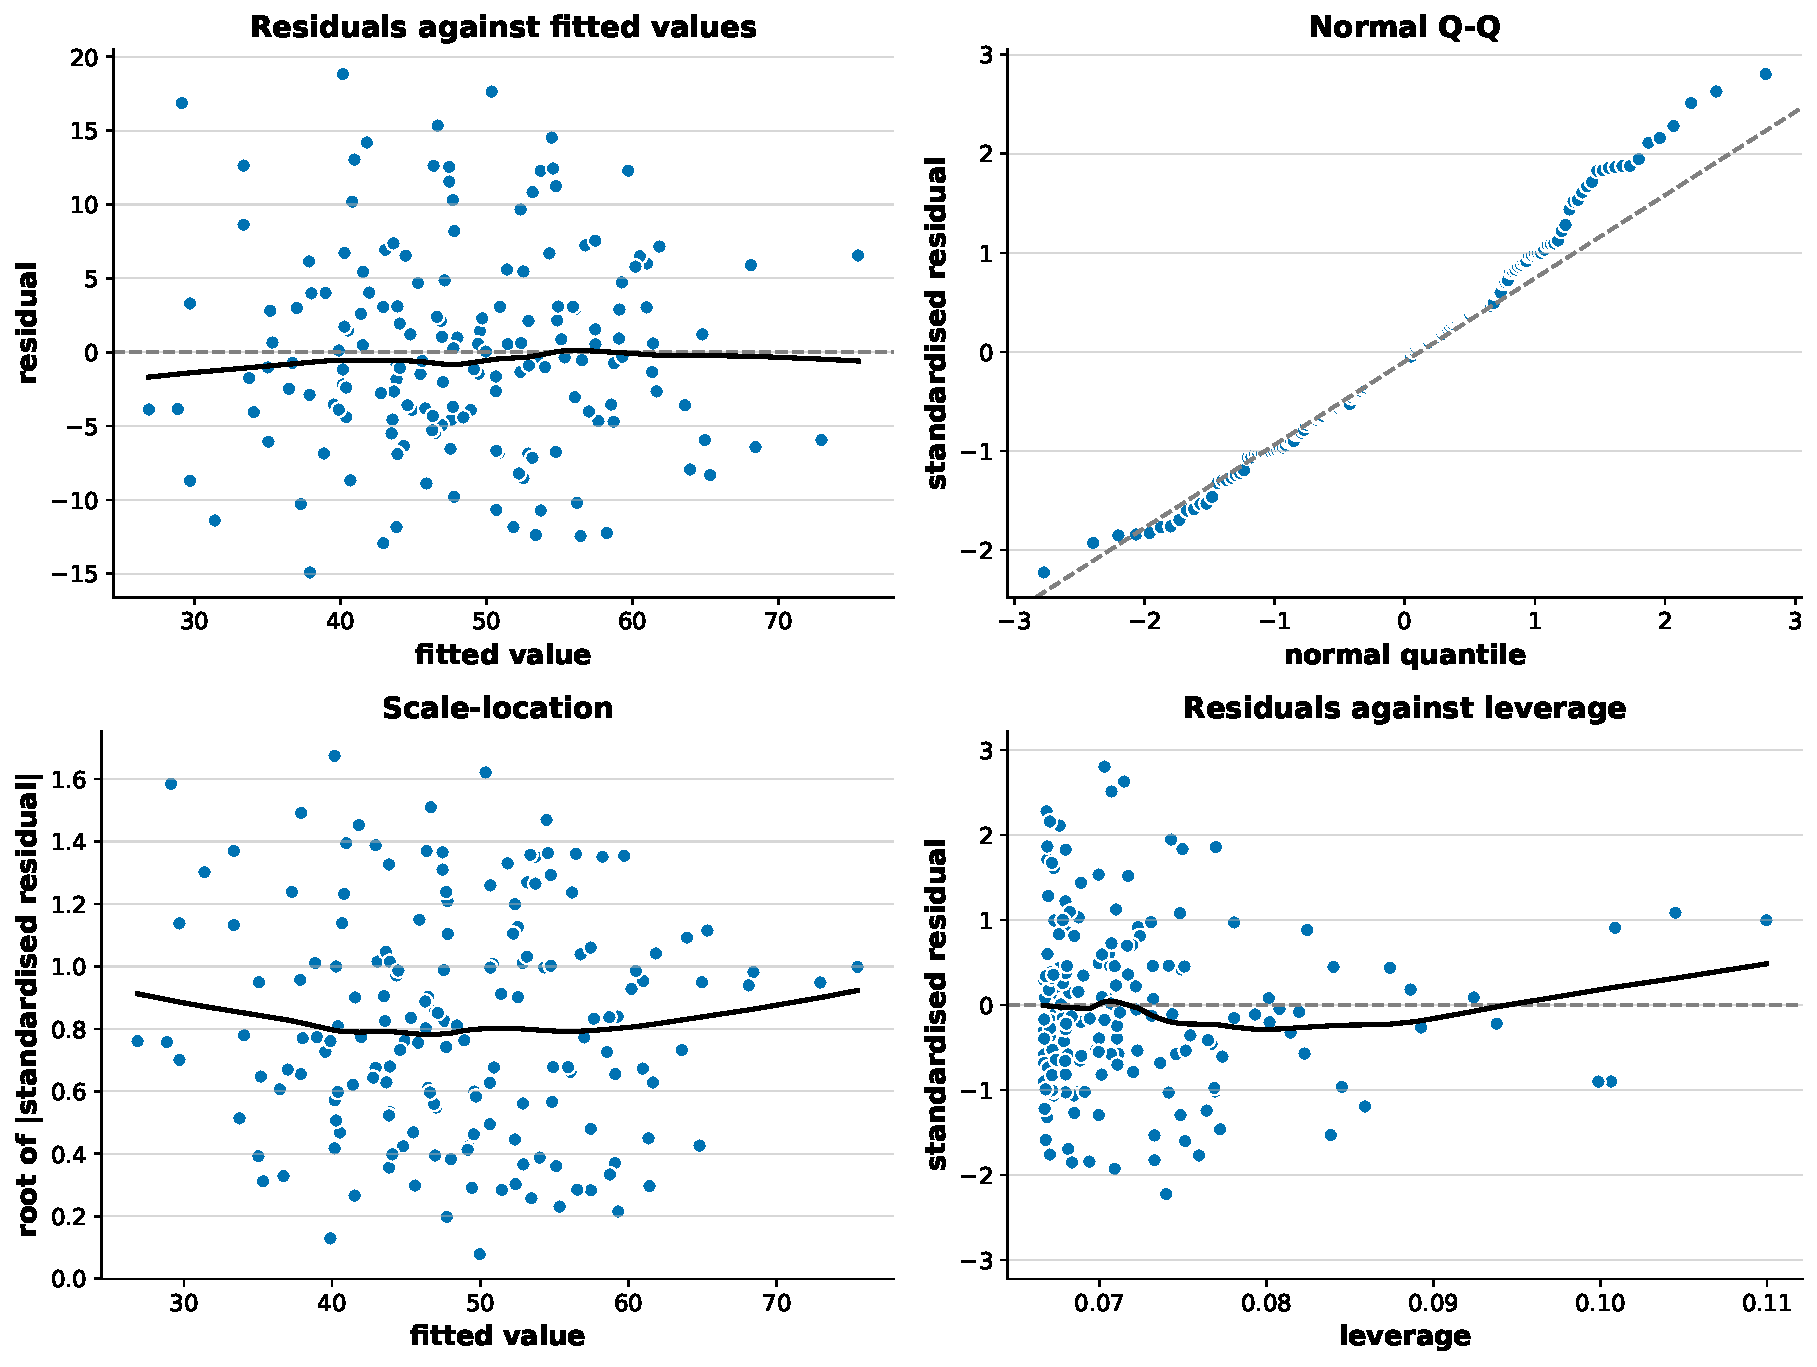
\includegraphics[width=0.52\textwidth,height=0.30\textheight,keepaspectratio]{figures/solution21_task2_model_checks.pdf}
\captionof*{figure}{Lesson 21, task 2: \code{model\_\allowbreak{}checks.\allowbreak{}png}.}
\end{minipage}\end{center}
\solutionanswer{The pictures look fine, and no row comes near the Cook's distance lines (the largest is 0.0457, row 97). Adding breakfast helps: F = 7.13, p = 0.008, and the AIC drops by 5.57.}
\solutiontask{3}{Try to remember without looking back: which word adds a prediction with its interval, and which option gives the interval for one new row? Use them to predict \code{\textquotedbl{}marks\textquotedbl{}} from \code{\textquotedbl{}hours\textquotedbl{}} and \code{\textquotedbl{}sleep\textquotedbl{}}, and look at the first 3 rows.}
\begin{lstlisting}[style=py]
import simplydata as sdata
table = sdata.table(sdata.get_example("school"))
table.add_predicted_column("marks", using=["hours", "sleep"], interval=95, for_new_rows=True)
table.keep_columns(contains="predicted")
table.show(rows=3)
\end{lstlisting}
\printedoutput{output/solution21_task3.txt}
\solutionanswer{\code{add\_\allowbreak{}predicted\_\allowbreak{}column} with \code{interval=95} and \code{for\_\allowbreak{}new\_\allowbreak{}rows=True}; \code{keep\_\allowbreak{}columns(contains=\textquotedbl{}predicted\textquotedbl{})} keeps the three new columns, and \code{show(rows=3)} shows the first 3 rows with every column. Pupil 1 is predicted 46.9, but one pupil like this could score from 29.8 to 64.0. Pupil 2 has no sleep value, so its cells stay empty.}
\solutiontask{4}{If you have R: find the model averages of \code{\textquotedbl{}marks\textquotedbl{}} for each \code{\textquotedbl{}school\textquotedbl{}}, allowing for \code{\textquotedbl{}hours\textquotedbl{}}. Which school has the highest average and which the lowest, and how many pairs of schools differ?}
\begin{lstlisting}[style=py]
import simplydata as sdata
table = sdata.table(sdata.get_example("school"))
table.find_model_averages_of("marks", for_each_group_in="school", using=["hours"])
\end{lstlisting}
\printedoutput{output/solution21_task4.txt}
\solutionanswer{With hours held at their average (5.00), School D has the highest average mark (57.7) and School C the lowest (36.5). 22 of the 66 pairs of schools differ after Tukey's adjustment (p \textless{} 0.05). This needs R (emmeans).}
\par\noindent{\small\sffamily\hyperref[lesson:21]{Back to lesson 21}}
\unsection{Lesson 22: Risks, diagnostic tests and agreement}{solutions:22}
\solutiontask{1}{Compare the risk of \code{\textquotedbl{}infected\textquotedbl{}} between the wards, against \code{\textquotedbl{}ward A\textquotedbl{}}. Does the interval of the difference leave out 0?}
\begin{lstlisting}[style=py]
import simplydata as sdata
table = sdata.table(sdata.get_example("clinic"))
table.compare_risks("infected", for_each_group_in="ward", against="ward A")
\end{lstlisting}
\printedoutput{output/solution22_task1.txt}
\solutionanswer{About 10 more in 100 in ward B, but the interval of the difference, -2.02 to 21.7 points, includes 0, so the data cannot tell (p = 0.142); the number needed runs through infinity.}
\solutiontask{2}{How good is the rapid test where only 2 \% have the infection? Of the positive results, how many really have it?}
\begin{lstlisting}[style=py]
import simplydata as sdata
table = sdata.table(sdata.get_example("clinic"))
table.compare_to_truth("rapid_test", truth="infected", prevalence=2)
\end{lstlisting}
\printedoutput{output/solution22_task2.txt}
\solutionanswer{Of 1000 people, 20 have it; the test finds 16 but 65 test positive by mistake, so only 16 of the 81 positives (about 1 in 5) are real.}
\solutiontask{3}{Complete the started lines to draw the two ratios of task 1: risks = \code{table.\allowbreak{}compare\_\allowbreak{}risks(\textquotedbl{}infected\textquotedbl{},\allowbreak{} for\_\allowbreak{}each\_\allowbreak{}group\_\allowbreak{}in=\textquotedbl{}ward\textquotedbl{},\allowbreak{} against=\textquotedbl{}ward A\textquotedbl{})}, then \code{risks.\allowbreak{}keep\_\allowbreak{}rows\_\allowbreak{}where(\textquotedbl{}measure\textquotedbl{},\allowbreak{} is\_\allowbreak{}one\_\allowbreak{}of=[.\allowbreak{}.\allowbreak{}.\allowbreak{}])}, then chart = \code{risks.\allowbreak{}start\_\allowbreak{}chart()} and \code{chart.\allowbreak{}forest\_\allowbreak{}plot(.\allowbreak{}.\allowbreak{}.\allowbreak{})}.}
\begin{lstlisting}[style=py]
import simplydata as sdata
table = sdata.table(sdata.get_example("clinic"))
risks = table.compare_risks("infected", for_each_group_in="ward", against="ward A")
risks.keep_rows_where("measure", is_one_of=["risk ratio", "odds ratio"])
chart = risks.start_chart()
chart.forest_plot(x="estimate", y="measure")
chart.save("infected_ratios.png")
\end{lstlisting}
\printedoutput{output/solution22_task3.txt}
\begin{center}\begin{minipage}{\linewidth}\centering
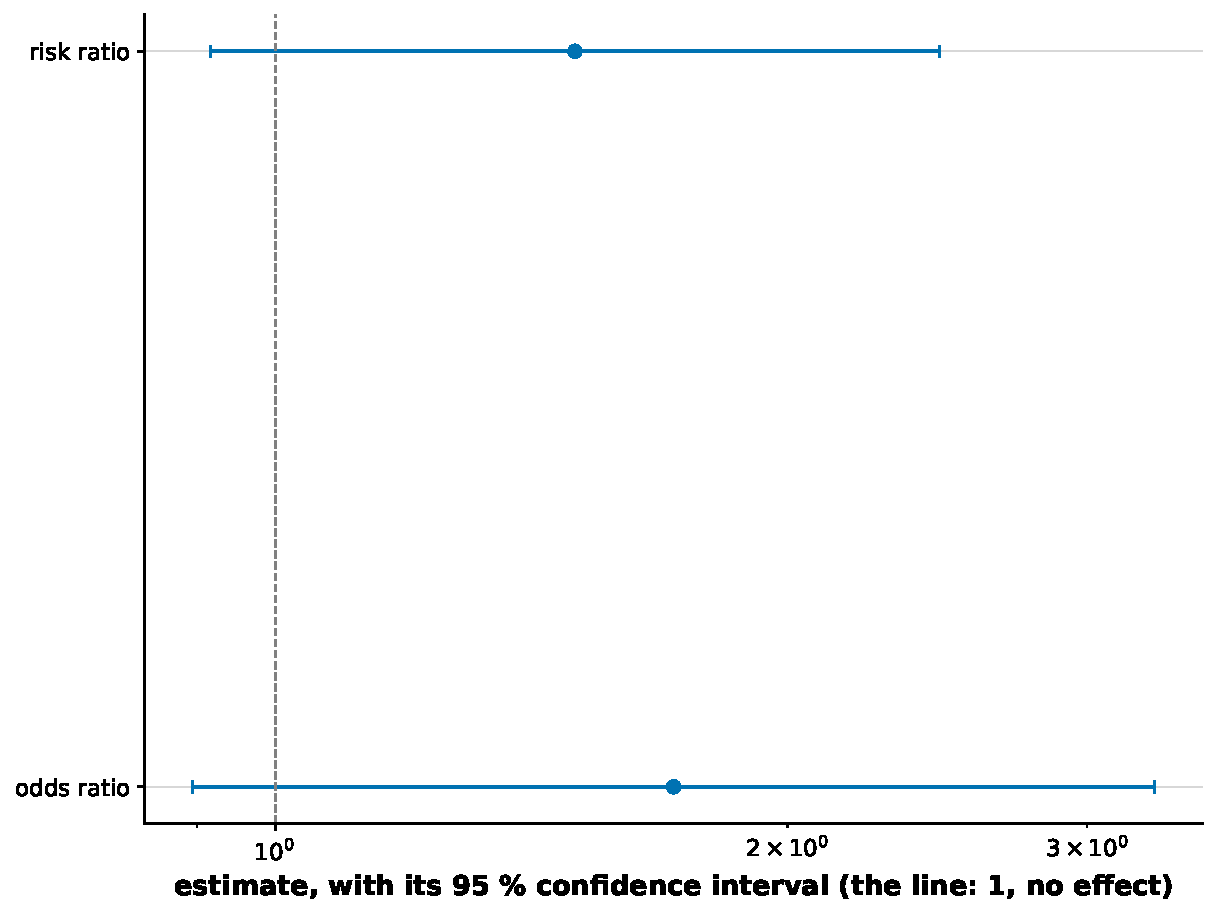
\includegraphics[width=0.52\textwidth,height=0.30\textheight,keepaspectratio]{figures/solution22_task3_infected_ratios.pdf}
\captionof*{figure}{Lesson 22, task 3: \code{infected\_\allowbreak{}ratios.\allowbreak{}png}.}
\end{minipage}\end{center}
\solutionanswer{Both intervals cross the line at 1, as the interval of the difference includes 0.}
\par\noindent{\small\sffamily\hyperref[lesson:22]{Back to lesson 22}}
\unsection{Lesson 23: Time series: dates, missing days, time windows and trend}{solutions:23}
\solutiontask{1}{Make a run of dates for every day of March 2026.}
\begin{lstlisting}[style=py]
import simplydata as sdata
days = sdata.make_run_of_dates("2026-03-01", to="2026-03-31", every="day")
days.show()
\end{lstlisting}
\printedoutput{output/solution23_task1.txt}
\solutionanswer{31 dates, one a day.}
\solutiontask{2}{Add a column with the average level of the last 30 days at each station.}
\begin{lstlisting}[style=py]
import simplydata as sdata
table = sdata.table(sdata.get_example("river"))
table.add_rolling_column("month_level", from_column="level", window="30 days", sorted_by="date", for_each_group_in="station")
table.show_first_rows()
\end{lstlisting}
\printedoutput{output/solution23_task2.txt}
\solutionanswer{A time window works even with missing days: it counts days, not rows.}
\solutiontask{3}{Smooth the level of each station with a moving average over 61 days instead of 31, and draw it. What does the wider window do?}
\begin{lstlisting}[style=py]
import simplydata as sdata
table = sdata.table(sdata.get_example("river"))
table.add_missing_dates("date", every="day", for_each_group_in="station")
table.fill_empty_cells_in("level", with_the="line between neighbours", sorted_by="date", for_each_group_in="station")
table.add_smoothed_column("level_smoothed", from_column="level", window=61, sorted_by="date", for_each_group_in="station")
chart = table.start_chart()
chart.draw_lines(x="date", y="level_smoothed", colour="station")
chart.save("level_smoothed.png")
\end{lstlisting}
\printedoutput{output/solution23_task3.txt}
\begin{center}\begin{minipage}{\linewidth}\centering
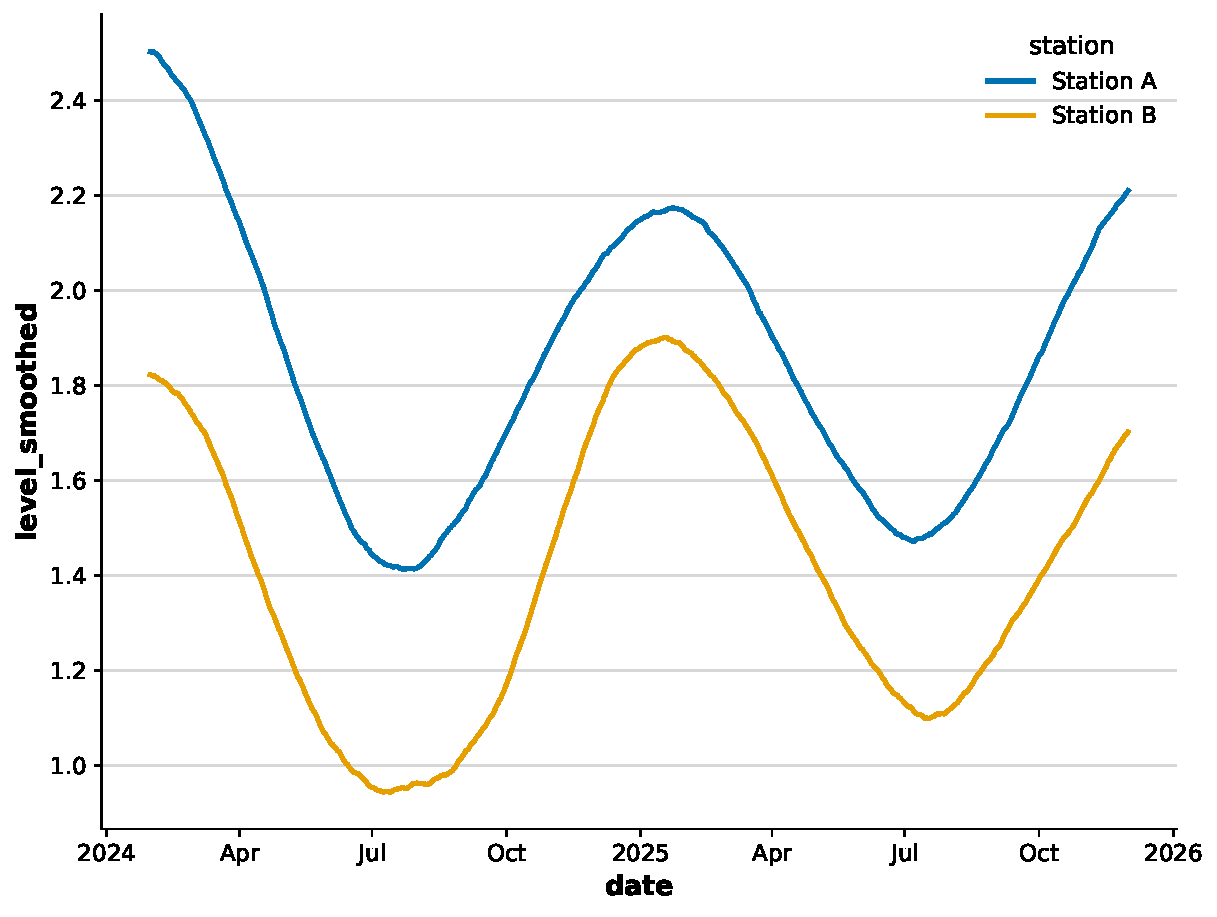
\includegraphics[width=0.52\textwidth,height=0.30\textheight,keepaspectratio]{figures/solution23_task3_level_smoothed.pdf}
\captionof*{figure}{Lesson 23, task 3: \code{level\_\allowbreak{}smoothed.\allowbreak{}png}.}
\end{minipage}\end{center}
\solutionanswer{The wider window gives a calmer line that hides the shorter ups and downs, and now the first and last 30 days of each station are empty.}
\par\noindent{\small\sffamily\hyperref[lesson:23]{Back to lesson 23}}
\unsection{Lesson 24: Forecasts: the next months, checked first}{solutions:24}
\solutiontask{1}{Forecast the Harbour Museum with \code{method=\textquotedbl{}same season last time\textquotedbl{}}. How does it compare with exponential smoothing?}
\begin{lstlisting}[style=py]
import simplydata as sdata
table = sdata.table(sdata.get_example("visitors"))
table.keep_rows_where("museum", is_equal_to="Harbour Museum")
table.forecast("visitors", sorted_by="month", steps_ahead=12, repeats_every="year", method="same season last time")
\end{lstlisting}
\printedoutput{output/solution24_task1.txt}
\solutionanswer{It repeats last year's months, so it misses the rise; \code{compare\_\allowbreak{}forecasts\_\allowbreak{}for} showed it is about twice as far off as exponential smoothing (MASE 0.930 against 0.469).}
\solutiontask{2}{Check the \code{\textquotedbl{}straight on\textquotedbl{}} method (the line from the first reading to the last) on the last 12 months of the Hill Gallery.}
\begin{lstlisting}[style=py]
import simplydata as sdata
table = sdata.table(sdata.get_example("visitors"))
table.keep_rows_where("museum", is_equal_to="Hill Gallery")
table.forecast("visitors", sorted_by="month", steps_ahead=12, method="straight on", check_on_last=12)
\end{lstlisting}
\printedoutput{output/solution24_task2.txt}
\solutionanswer{It follows the rise but not the season: far worse than exponential smoothing (MASE 2.08 in \code{compare\_\allowbreak{}forecasts\_\allowbreak{}for}).}
\par\noindent{\small\sffamily\hyperref[lesson:24]{Back to lesson 24}}
\unsection{Lesson 25: Cycles: spectra, filters, peaks, and steady or not}{solutions:25}
\solutiontask{1}{Which cycle is strongest in the \code{\textquotedbl{}vibration\textquotedbl{}} column? Is it the same as in \code{\textquotedbl{}signal\textquotedbl{}}?}
\begin{lstlisting}[style=py]
import simplydata as sdata
table = sdata.table(sdata.get_example("sensor"))
table.find_spectrum_of("vibration", sorted_by="time")
\end{lstlisting}
\printedoutput{output/solution25_task1.txt}
\solutionanswer{The same: 5 per second (65 \% of the variance), then 20 per second and the 50-per-second hum. The vibration follows the signal, a little later.}
\solutiontask{2}{Keep only the frequencies between 15 and 25 in the signal. Which cycle is left?}
\begin{lstlisting}[style=py]
import simplydata as sdata
table = sdata.table(sdata.get_example("sensor"))
table.add_filtered_column("middle", from_column="signal", keep_between=[15, 25], sorted_by="time")
table.find_spectrum_of("middle", sorted_by="time")
\end{lstlisting}
\printedoutput{output/solution25_task2.txt}
\solutionanswer{Only the 20-per-second cycle is left: it holds 89 \% of the variance of the new column.}
\solutiontask{3}{Find the dips of the signal that go down to -1.5 or lower. Is the lowest one still the same?}
\begin{lstlisting}[style=py]
import simplydata as sdata
table = sdata.table(sdata.get_example("sensor"))
table.find_each_dip_that("signal", sorted_by="time", is_at_most=-1.5)
\end{lstlisting}
\printedoutput{output/solution25_task3.txt}
\solutionanswer{Many more dips now, each with its time and value; the lowest is still -2.36 at time 0.94.}
\par\noindent{\small\sffamily\hyperref[lesson:25]{Back to lesson 25}}
\unsection{Lesson 26: Systems: a spring and damper, its response and a feedback loop}{solutions:26}
\solutiontask{1}{Make the damper stronger: 1 / (s**2 + 2*s + 4). What happens to the overshoot?}
\begin{lstlisting}[style=py]
import simplydata as sdata
spring = sdata.system("1 / (s**2 + 2*s + 4)")
spring.step_response(until=15)
\end{lstlisting}
\printedoutput{output/solution26_task1.txt}
\solutionanswer{Damping ratio 0.5 instead of 0.2: the overshoot drops to about 16 \%.}
\solutiontask{2}{Use a controller that only pushes in proportion to the error, \code{sdata.\allowbreak{}system(\textquotedbl{}10\textquotedbl{})}. Where does the position settle?}
\begin{lstlisting}[style=py]
import simplydata as sdata
spring = sdata.system("1 / (s**2 + 0.8*s + 4)")
loop = sdata.system("10").then(spring).with_feedback()
loop.step_response(until=30)
\end{lstlisting}
\printedoutput{output/solution26_task2.txt}
\solutionanswer{It settles at 0.714, not at 1: a push in proportion to the error always leaves some error. The part that adds up the error over time removes it.}
\solutiontask{3}{Draw the poles and zeros of the closed loop of part 3.}
\begin{lstlisting}[style=py]
import simplydata as sdata
spring = sdata.system("1 / (s**2 + 0.8*s + 4)")
loop = sdata.system("2 * (s + 1) / s").then(spring).with_feedback()
chart = loop.chart(show="poles and zeros")
chart.save("loop_poles.png")
\end{lstlisting}
\printedoutput{output/solution26_task3.txt}
\begin{center}\begin{minipage}{\linewidth}\centering
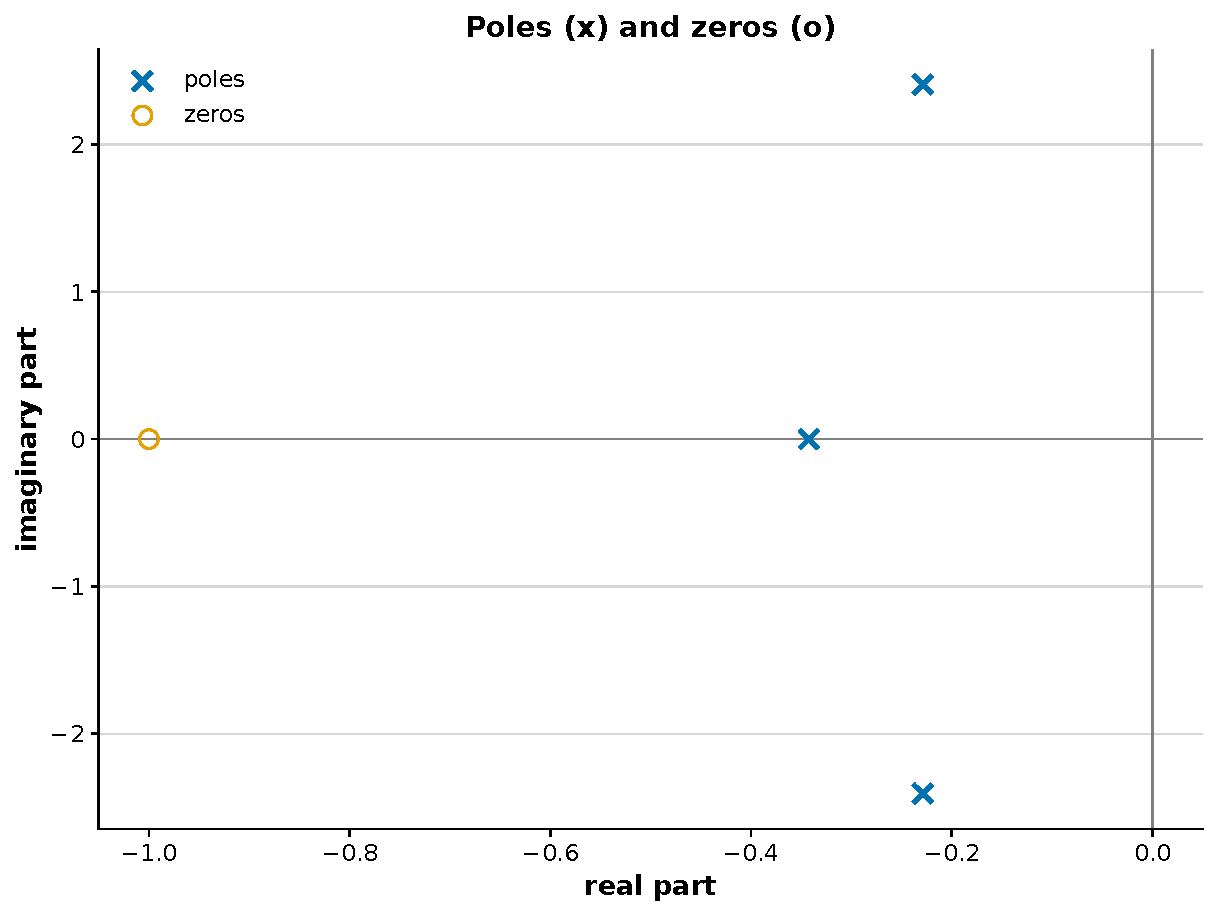
\includegraphics[width=0.52\textwidth,height=0.30\textheight,keepaspectratio]{figures/solution26_task3_loop_poles.pdf}
\captionof*{figure}{Lesson 26, task 3: \code{loop\_\allowbreak{}poles.\allowbreak{}png}.}
\end{minipage}\end{center}
\solutionanswer{Three poles, all left of the imaginary axis (stable), and one zero at -1.}
\par\noindent{\small\sffamily\hyperref[lesson:26]{Back to lesson 26}}
\unsection{Lesson 27: Beyond the average line: outliers}{solutions:27}
\solutiontask{1}{In the marks table, explain \code{\textquotedbl{}marks\textquotedbl{}} from \code{\textquotedbl{}hours\textquotedbl{}} with \code{giving\_\allowbreak{}outliers\_\allowbreak{}less\_\allowbreak{}weight=True}. Which rows get less weight?}
\begin{lstlisting}[style=py]
import simplydata as sdata
table = sdata.table(sdata.get_example("marks"))
table.explain("marks", using=["hours"], giving_outliers_less_weight=True)
\end{lstlisting}
\printedoutput{output/solution27_task1.txt}
\solutionanswer{Four rows get less weight: row 22 (weight 0.59), then rows 45, 11 and 42. The printout lists them with the lowest weight first.}
\solutiontask{2}{Without looking back: which option changes the effects themselves, \code{giving\_\allowbreak{}outliers\_\allowbreak{}less\_\allowbreak{}weight=} or \code{robust\_\allowbreak{}errors=}? Run both on the school table to check.}
\begin{lstlisting}[style=py]
import simplydata as sdata
table = sdata.table(sdata.get_example("school"))
table.explain("marks", using=["hours"], giving_outliers_less_weight=True)
table.explain("marks", using=["hours"], robust_errors=True)
\end{lstlisting}
\printedoutput{output/solution27_task2.txt}
\solutionanswer{\code{giving\_\allowbreak{}outliers\_\allowbreak{}less\_\allowbreak{}weight=} changes the effects (rows far from the model count less); \code{robust\_\allowbreak{}errors=} gives the same effects as the ordinary model, with other standard errors.}
\par\noindent{\small\sffamily\hyperref[lesson:27]{Back to lesson 27}}

\backmatter

\unchapter{Index of words}{index}
Every word and option, A to Z, with the page of its dictionary entry. Other spellings of a word (such as \code{chart.\allowbreak{}use\_\allowbreak{}color()} for \code{chart.\allowbreak{}use\_\allowbreak{}colour()}) point to the same entry.
\begin{multicols}{2}\small\raggedright\setlength{\parskip}{0.1em}
\indexline{word:nums.add}{nums.add()}
\indexline{word:system.add}{system.add()}
\indexline{word:table.add-adjusted-p-value-column}{table.add\_adjusted\_p\_value\_column()}
\indexline{word:table.add-change-column}{table.add\_change\_column()}
\indexline{word:table.add-clusters}{table.add\_clusters()}
\indexline{word:table.add-column}{table.add\_column()}
\indexline{word:table.add-column-with-part-of-date}{table.add\_column\_with\_part\_of\_date()}
\indexline{word:table.add-column-with-part-of-text}{table.add\_column\_with\_part\_of\_text()}
\indexline{word:table.add-envelope-column}{table.add\_envelope\_column()}
\indexline{word:table.add-filtered-column}{table.add\_filtered\_column()}
\indexline{word:table.add-group-column}{table.add\_group\_column()}
\indexline{word:table.add-is-empty-column}{table.add\_is\_empty\_column()}
\indexline{word:table.add-missing-dates}{table.add\_missing\_dates()}
\indexline{word:table.add-nmds}{table.add\_nmds()}
\indexline{word:table.add-predicted-column}{table.add\_predicted\_column()}
\indexline{word:table.add-previous-value-column}{table.add\_previous\_value\_column()}
\indexline{word:table.add-principal-components}{table.add\_principal\_components()}
\indexline{word:table.add-rank-column}{table.add\_rank\_column()}
\indexline{word:table.add-rolling-column}{table.add\_rolling\_column()}
\indexline{word:table.add-rows-from}{table.add\_rows\_from()}
\indexline{word:add-second-y}{chart.add\_second\_y()}
\indexline{word:table.add-smoothed-column}{table.add\_smoothed\_column()}
\indexline{word:table.add-trend-and-season}{table.add\_trend\_and\_season()}
\indexline{word:table.add-z-score-column}{table.add\_z\_score\_column()}
\indexline{word:add-zoom-box}{chart.add\_zoom\_box()}
\indexline{word:table.agreement-between}{table.agreement\_between()}
\indexline{word:animate}{chart.animate()}
\indexline{word:nums.as-numpy}{nums.as\_numpy()}
\indexline{word:table.as-pandas}{table.as\_pandas()}
\indexline{word:table.as-polars}{table.as\_polars()}
\indexline{word:autocorrelation-bars}{chart.autocorrelation\_bars()}
\indexline{word:table.change-column}{table.change\_column()}
\indexline{word:nums.change-time-step}{nums.change\_time\_step()}
\indexline{word:sdata.chart}{sdata.chart()}
\indexline{word:system.chart}{system.chart()}
\indexline{word:table.check-if-random-order}{table.check\_if\_random\_order()}
\indexline{word:table.check-model-of}{table.check\_model\_of()}
\indexline{word:table.check-steady-over-time}{table.check\_steady\_over\_time()}
\indexline{word:table.compare-accuracy}{table.compare\_accuracy()}
\indexline{word:table.compare-average-to}{table.compare\_average\_to()}
\indexline{word:sdata.compare-averages}{sdata.compare\_averages()}
\indexline{word:table.compare-averages-of}{table.compare\_averages\_of()}
\indexline{word:table.compare-before-and-after}{table.compare\_before\_and\_after()}
\indexline{word:table.compare-correlations}{table.compare\_correlations()}
\indexline{word:sdata.compare-counts}{sdata.compare\_counts()}
\indexline{word:table.compare-counts-of}{table.compare\_counts\_of()}
\indexline{word:table.compare-counts-to}{table.compare\_counts\_to()}
\indexline{word:table.compare-distributions-for}{table.compare\_distributions\_for()}
\indexline{word:table.compare-each-pair-of}{table.compare\_each\_pair\_of()}
\indexline{word:table.compare-forecasts-for}{table.compare\_forecasts\_for()}
\indexline{word:table.compare-matched-columns}{table.compare\_matched\_columns()}
\indexline{word:table.compare-models}{table.compare\_models()}
\indexline{word:table.compare-percent-to}{table.compare\_percent\_to()}
\indexline{word:table.compare-profiles-of}{table.compare\_profiles\_of()}
\indexline{word:sdata.compare-rates}{sdata.compare\_rates()}
\indexline{word:table.compare-rates}{table.compare\_rates()}
\indexline{word:sdata.compare-risks}{sdata.compare\_risks()}
\indexline{word:table.compare-risks}{table.compare\_risks()}
\indexline{word:table.compare-shape-to}{table.compare\_shape\_to()}
\indexline{word:table.compare-shapes-of}{table.compare\_shapes\_of()}
\indexline{word:table.compare-spreads-of}{table.compare\_spreads\_of()}
\indexline{word:table.compare-survival}{table.compare\_survival()}
\indexline{word:sdata.compare-to-truth}{sdata.compare\_to\_truth()}
\indexline{word:table.compare-to-truth}{table.compare\_to\_truth()}
\indexline{word:nums.convolve-with}{nums.convolve\_with()}
\indexline{word:nums.count}{nums.count()}
\indexline{word:grid.count-columns}{grid.count\_columns()}
\indexline{word:table.count-different-values-in}{table.count\_different\_values\_in()}
\indexline{word:nums.count-each}{nums.count\_each()}
\indexline{word:table.count-each}{table.count\_each()}
\indexline{word:table.count-empty-cells-in}{table.count\_empty\_cells\_in()}
\indexline{word:nums.count-empty-numbers}{nums.count\_empty\_numbers()}
\indexline{word:grid.count-rows}{grid.count\_rows()}
\indexline{word:table.count-rows}{table.count\_rows()}
\indexline{word:cross-correlation-bars}{chart.cross\_correlation\_bars()}
\indexline{word:nums.deconvolve-by}{nums.deconvolve\_by()}
\indexline{word:table.describe-columns}{table.describe\_columns()}
\indexline{word:difference-dots}{chart.difference\_dots()}
\indexline{word:sdata.distribution}{sdata.distribution()}
\indexline{word:nums.divide-by}{nums.divide\_by()}
\indexline{word:draw-all-dots}{chart.draw\_all\_dots()}
\indexline{word:sdata.draw-all-pairs}{sdata.draw\_all\_pairs()}
\indexline{word:draw-area}{chart.draw\_area()}
\indexline{word:draw-band}{chart.draw\_band()}
\indexline{word:draw-bars}{chart.draw\_bars()}
\indexline{word:draw-boxes}{chart.draw\_boxes()}
\indexline{word:dist.draw-chart}{dist.draw\_chart()}
\indexline{word:draw-contour}{chart.draw\_contour()}
\indexline{word:draw-count-bars}{chart.draw\_count\_bars()}
\indexline{word:draw-cumulative-share}{chart.draw\_cumulative\_share()}
\indexline{word:draw-curve}{chart.draw\_curve()}
\indexline{word:draw-density}{chart.draw\_density()}
\indexline{word:draw-dots}{chart.draw\_dots()}
\indexline{word:draw-dots-3d}{chart.draw\_dots\_3d()}
\indexline{word:draw-error-bars}{chart.draw\_error\_bars()}
\indexline{word:draw-heatmap}{chart.draw\_heatmap()}
\indexline{word:draw-histogram}{chart.draw\_histogram()}
\indexline{word:draw-line-at-x}{chart.draw\_line\_at\_x()}
\indexline{word:draw-line-at-y}{chart.draw\_line\_at\_y()}
\indexline{word:draw-line-with-slope}{chart.draw\_line\_with\_slope()}
\indexline{word:draw-lines}{chart.draw\_lines()}
\indexline{word:draw-map-of-empty-cells}{chart.draw\_map\_of\_empty\_cells()}
\indexline{word:draw-one-chart-for-each-group-in}{chart.draw\_one\_chart\_for\_each\_group\_in()}
\indexline{word:draw-pie}{chart.draw\_pie()}
\indexline{word:draw-polar}{chart.draw\_polar()}
\indexline{word:draw-qq-dots}{chart.draw\_qq\_dots()}
\indexline{word:draw-side-histograms}{chart.draw\_side\_histograms()}
\indexline{word:draw-smooth-line}{chart.draw\_smooth\_line()}
\indexline{word:draw-surface}{chart.draw\_surface()}
\indexline{word:draw-survival-curves}{chart.draw\_survival\_curves()}
\indexline{word:draw-violins}{chart.draw\_violins()}
\indexline{word:error-eq}{error=}
\indexline{word:table.explain}{table.explain()}
\indexline{word:table.explain-survival}{table.explain\_survival()}
\indexline{word:table.fill-empty-cells-in}{table.fill\_empty\_cells\_in()}
\indexline{word:nums.fill-empty-numbers}{nums.fill\_empty\_numbers()}
\indexline{word:nums.find-autocorrelation}{nums.find\_autocorrelation()}
\indexline{word:table.find-autocorrelation-of}{table.find\_autocorrelation\_of()}
\indexline{word:dist.find-average}{dist.find\_average()}
\indexline{word:nums.find-average}{nums.find\_average()}
\indexline{word:table.find-average-of}{table.find\_average\_of()}
\indexline{word:nums.find-biggest}{nums.find\_biggest()}
\indexline{word:table.find-biggest-of}{table.find\_biggest\_of()}
\indexline{word:sdata.find-chance-of-finding}{sdata.find\_chance\_of\_finding()}
\indexline{word:dist.find-chance-that-value}{dist.find\_chance\_that\_value()}
\indexline{word:table.find-change-points-in}{table.find\_change\_points\_in()}
\indexline{word:table.find-correlation-between}{table.find\_correlation\_between()}
\indexline{word:dist.find-cut-off}{dist.find\_cut\_off()}
\indexline{word:dist.find-density-at}{dist.find\_density\_at()}
\indexline{word:table.find-distances-between-rows}{table.find\_distances\_between\_rows()}
\indexline{word:nums.find-each-dip-that}{nums.find\_each\_dip\_that()}
\indexline{word:table.find-each-dip-that}{table.find\_each\_dip\_that()}
\indexline{word:nums.find-each-peak-that}{nums.find\_each\_peak\_that()}
\indexline{word:table.find-each-peak-that}{table.find\_each\_peak\_that()}
\indexline{word:nums.find-envelope}{nums.find\_envelope()}
\indexline{word:sdata.find-how-many-needed}{sdata.find\_how\_many\_needed()}
\indexline{word:table.find-interval-of}{table.find\_interval\_of()}
\indexline{word:sdata.find-inverse-fourier-transform}{sdata.find\_inverse\_fourier\_transform()}
\indexline{word:dist.find-median}{dist.find\_median()}
\indexline{word:nums.find-median}{nums.find\_median()}
\indexline{word:table.find-median-of}{table.find\_median\_of()}
\indexline{word:dist.find-middle-range}{dist.find\_middle\_range()}
\indexline{word:table.find-model-averages-of}{table.find\_model\_averages\_of()}
\indexline{word:table.find-most-common-of}{table.find\_most\_common\_of()}
\indexline{word:table.find-percent-of-rows-where}{table.find\_percent\_of\_rows\_where()}
\indexline{word:dist.find-percentile}{dist.find\_percentile()}
\indexline{word:nums.find-percentile}{nums.find\_percentile()}
\indexline{word:table.find-percentile-of}{table.find\_percentile\_of()}
\indexline{word:table.find-principal-components-of}{table.find\_principal\_components\_of()}
\indexline{word:grid.find-shape}{grid.find\_shape()}
\indexline{word:nums.find-smallest}{nums.find\_smallest()}
\indexline{word:table.find-smallest-of}{table.find\_smallest\_of()}
\indexline{word:nums.find-spectrum}{nums.find\_spectrum()}
\indexline{word:table.find-spectrum-of}{table.find\_spectrum\_of()}
\indexline{word:dist.find-standard-deviation}{dist.find\_standard\_deviation()}
\indexline{word:nums.find-standard-deviation}{nums.find\_standard\_deviation()}
\indexline{word:table.find-standard-deviation-of}{table.find\_standard\_deviation\_of()}
\indexline{word:table.find-summary-of}{table.find\_summary\_of()}
\indexline{word:table.find-survival-over-time}{table.find\_survival\_over\_time()}
\indexline{word:nums.find-total}{nums.find\_total()}
\indexline{word:table.find-total-of}{table.find\_total\_of()}
\indexline{word:table.find-trend-of}{table.find\_trend\_of()}
\indexline{word:dist.find-variance}{dist.find\_variance()}
\indexline{word:sdata.find-where-biggest}{sdata.find\_where\_biggest()}
\indexline{word:sdata.find-where-smallest}{sdata.find\_where\_smallest()}
\indexline{word:fit-curve}{chart.fit\_curve()}
\indexline{word:table.fit-curve}{table.fit\_curve()}
\indexline{word:fit-distribution}{chart.fit\_distribution()}
\indexline{word:nums.fit-distribution}{nums.fit\_distribution()}
\indexline{word:table.fit-distribution-to}{table.fit\_distribution\_to()}
\indexline{word:fit-formula}{chart.fit\_formula()}
\indexline{word:table.fit-formula}{table.fit\_formula()}
\indexline{word:fit-line}{chart.fit\_line()}
\indexline{word:table.fit-line}{table.fit\_line()}
\indexline{word:flip-x}{chart.flip\_x()}
\indexline{word:flip-y}{chart.flip\_y()}
\indexline{word:forecast}{chart.forecast()}
\indexline{word:nums.forecast}{nums.forecast()}
\indexline{word:table.forecast}{table.forecast()}
\indexline{word:forest-plot}{chart.forest\_plot()}
\indexline{word:sdata.frequency-filter}{sdata.frequency\_filter()}
\indexline{word:system.frequency-response}{system.frequency\_response()}
\indexline{word:grid.get-all-numbers}{grid.get\_all\_numbers()}
\indexline{word:table.get-cell-at}{table.get\_cell\_at()}
\indexline{word:grid.get-column}{grid.get\_column()}
\indexline{word:table.get-column}{table.get\_column()}
\indexline{word:table.get-column-names}{table.get\_column\_names()}
\indexline{word:sdata.get-example}{sdata.get\_example()}
\indexline{word:grid.get-number-at}{grid.get\_number\_at()}
\indexline{word:nums.get-number-at}{nums.get\_number\_at()}
\indexline{word:grid.get-row}{grid.get\_row()}
\indexline{word:table.get-row}{table.get\_row()}
\indexline{word:sdata.go-to-next-day}{sdata.go\_to\_next\_day()}
\indexline{word:sdata.help}{sdata.help()}
\indexline{word:hide-grid}{chart.hide\_grid()}
\indexline{word:hide-legend}{chart.hide\_legend()}
\indexline{word:system.impulse-response}{system.impulse\_response()}
\indexline{word:system.in-steps}{system.in\_steps()}
\indexline{word:system.is-stable}{system.is\_stable()}
\indexline{word:table.join-with}{table.join\_with()}
\indexline{word:table.keep-biggest-rows}{table.keep\_biggest\_rows()}
\indexline{word:table.keep-columns}{table.keep\_columns()}
\indexline{word:grid.keep-columns-by-position}{grid.keep\_columns\_by\_position()}
\indexline{word:table.keep-columns-by-position}{table.keep\_columns\_by\_position()}
\indexline{word:nums.keep-each-frequency-that}{nums.keep\_each\_frequency\_that()}
\indexline{word:nums.keep-each-number-that}{nums.keep\_each\_number\_that()}
\indexline{word:nums.keep-first-numbers}{nums.keep\_first\_numbers()}
\indexline{word:table.keep-first-rows}{table.keep\_first\_rows()}
\indexline{word:nums.keep-last-numbers}{nums.keep\_last\_numbers()}
\indexline{word:table.keep-last-rows}{table.keep\_last\_rows()}
\indexline{word:nums.keep-numbers-by-position}{nums.keep\_numbers\_by\_position()}
\indexline{word:nums.keep-random-numbers}{nums.keep\_random\_numbers()}
\indexline{word:table.keep-random-rows}{table.keep\_random\_rows()}
\indexline{word:grid.keep-rows-by-position}{grid.keep\_rows\_by\_position()}
\indexline{word:table.keep-rows-by-position}{table.keep\_rows\_by\_position()}
\indexline{word:table.keep-rows-where}{table.keep\_rows\_where()}
\indexline{word:table.keep-smallest-rows}{table.keep\_smallest\_rows()}
\indexline{word:label-colour-bar}{chart.label\_color\_bar()}
\indexline{word:label-colour-bar}{chart.label\_colour\_bar()}
\indexline{word:label-legend}{chart.label\_legend()}
\indexline{word:label-x}{chart.label\_x()}
\indexline{word:label-y}{chart.label\_y()}
\indexline{word:lag-dots}{chart.lag\_dots()}
\indexline{word:table.limits-of-agreement}{table.limits\_of\_agreement()}
\indexline{word:table.make-map-of}{table.make\_map\_of()}
\indexline{word:nums.make-number-grid}{nums.make\_number\_grid()}
\indexline{word:dist.make-random-numbers}{dist.make\_random\_numbers()}
\indexline{word:sdata.make-random-numbers}{sdata.make\_random\_numbers()}
\indexline{word:sdata.make-run-of-dates}{sdata.make\_run\_of\_dates()}
\indexline{word:sdata.make-wave}{sdata.make\_wave()}
\indexline{word:sdata.make-window-shape}{sdata.make\_window\_shape()}
\indexline{word:sdata.number-grid}{sdata.number\_grid()}
\indexline{word:sdata.numbers}{sdata.numbers()}
\indexline{word:order-legend}{chart.order\_legend()}
\indexline{word:order-x}{chart.order\_x()}
\indexline{word:order-y}{chart.order\_y()}
\indexline{word:peak-dots}{chart.peak\_dots()}
\indexline{word:system.poles}{system.poles()}
\indexline{word:sdata.put-in-rows-and-columns}{sdata.put\_in\_rows\_and\_columns()}
\indexline{word:put-legend-at-bottom}{chart.put\_legend\_at\_bottom()}
\indexline{word:put-legend-on-left}{chart.put\_legend\_at\_left()}
\indexline{word:put-legend-on-right}{chart.put\_legend\_at\_right()}
\indexline{word:put-legend-at-top}{chart.put\_legend\_at\_top()}
\indexline{word:put-legend-at-bottom}{chart.put\_legend\_on\_bottom()}
\indexline{word:put-legend-on-left}{chart.put\_legend\_on\_left()}
\indexline{word:put-legend-on-right}{chart.put\_legend\_on\_right()}
\indexline{word:put-legend-at-top}{chart.put\_legend\_on\_top()}
\indexline{word:sdata.put-one-above-other}{sdata.put\_one\_above\_other()}
\indexline{word:sdata.put-side-by-side}{sdata.put\_side\_by\_side()}
\indexline{word:put-ticks-x}{chart.put\_ticks\_x()}
\indexline{word:put-ticks-y}{chart.put\_ticks\_y()}
\indexline{word:nums.raise-to-power}{nums.raise\_to\_power()}
\indexline{word:table.rate-of}{table.rate\_of()}
\indexline{word:table.reliability-of}{table.reliability\_of()}
\indexline{word:table.remove-columns}{table.remove\_columns()}
\indexline{word:grid.remove-columns-by-position}{grid.remove\_columns\_by\_position()}
\indexline{word:table.remove-columns-by-position}{table.remove\_columns\_by\_position()}
\indexline{word:nums.remove-duplicate-numbers}{nums.remove\_duplicate\_numbers()}
\indexline{word:table.remove-duplicate-rows}{table.remove\_duplicate\_rows()}
\indexline{word:nums.remove-each-frequency-that}{nums.remove\_each\_frequency\_that()}
\indexline{word:nums.remove-each-number-that}{nums.remove\_each\_number\_that()}
\indexline{word:nums.remove-empty-numbers}{nums.remove\_empty\_numbers()}
\indexline{word:table.remove-extra-spaces-in}{table.remove\_extra\_spaces\_in()}
\indexline{word:nums.remove-numbers-by-position}{nums.remove\_numbers\_by\_position()}
\indexline{word:grid.remove-rows-by-position}{grid.remove\_rows\_by\_position()}
\indexline{word:table.remove-rows-by-position}{table.remove\_rows\_by\_position()}
\indexline{word:table.remove-rows-where}{table.remove\_rows\_where()}
\indexline{word:table.remove-rows-with-empty-cells-in}{table.remove\_rows\_with\_empty\_cells\_in()}
\indexline{word:table.remove-rows-with-outliers}{table.remove\_rows\_with\_outliers()}
\indexline{word:nums.remove-trend}{nums.remove\_trend()}
\indexline{word:table.rename-column}{table.rename\_column()}
\indexline{word:grid.replace-each-number-that}{grid.replace\_each\_number\_that()}
\indexline{word:nums.replace-each-number-that}{nums.replace\_each\_number\_that()}
\indexline{word:table.replace-text-in}{table.replace\_text\_in()}
\indexline{word:table.replace-values-in}{table.replace\_values\_in()}
\indexline{word:system.response-to}{system.response\_to()}
\indexline{word:nums.reverse}{nums.reverse()}
\indexline{word:table.reverse-rows}{table.reverse\_rows()}
\indexline{word:rotate-labels-x}{chart.rotate\_labels\_x()}
\indexline{word:rotate-labels-y}{chart.rotate\_labels\_y()}
\indexline{word:table.round-numbers-in}{table.round\_numbers\_in()}
\indexline{word:nums.round-to}{nums.round\_to()}
\indexline{word:save}{chart.save()}
\indexline{word:nums.save}{nums.save()}
\indexline{word:table.save}{table.save()}
\indexline{word:set-range-x}{chart.set\_range\_x()}
\indexline{word:set-range-y}{chart.set\_range\_y()}
\indexline{word:set-size}{chart.set\_size()}
\indexline{word:shade-between-x}{chart.shade\_between\_x()}
\indexline{word:shade-between-y}{chart.shade\_between\_y()}
\indexline{word:show}{chart.show()}
\indexline{word:nums.show}{nums.show()}
\indexline{word:show-eq}{show=}
\indexline{word:table.show}{table.show()}
\indexline{word:sdata.show-all-words}{sdata.show\_all\_words()}
\indexline{word:sdata.show-answers}{sdata.show\_answers()}
\indexline{word:sdata.show-day}{sdata.show\_day()}
\indexline{word:nums.show-first-numbers}{nums.show\_first\_numbers()}
\indexline{word:grid.show-first-rows}{grid.show\_first\_rows()}
\indexline{word:table.show-first-rows}{table.show\_first\_rows()}
\indexline{word:show-grid}{chart.show\_grid()}
\indexline{word:nums.show-last-numbers}{nums.show\_last\_numbers()}
\indexline{word:grid.show-last-rows}{grid.show\_last\_rows()}
\indexline{word:table.show-last-rows}{table.show\_last\_rows()}
\indexline{word:show-legend}{chart.show\_legend()}
\indexline{word:sdata.show-lesson}{sdata.show\_lesson()}
\indexline{word:dist.show-parameters}{dist.show\_parameters()}
\indexline{word:table.show-rows-that-pull-model}{table.show\_rows\_that\_pull\_model()}
\indexline{word:table.show-rows-with-outliers}{table.show\_rows\_with\_outliers()}
\indexline{word:nums.show-steps}{nums.show\_steps()}
\indexline{word:table.show-steps}{table.show\_steps()}
\indexline{word:dist.show-summary}{dist.show\_summary()}
\indexline{word:sdata.show-today}{sdata.show\_today()}
\indexline{word:nums.smooth}{nums.smooth()}
\indexline{word:sdata.solve}{sdata.solve()}
\indexline{word:nums.sort}{nums.sort()}
\indexline{word:table.sort-by}{table.sort\_by()}
\indexline{word:spectrum}{chart.spectrum()}
\indexline{word:spectrum-over-time}{chart.spectrum\_over\_time()}
\indexline{word:table.split-column}{table.split\_column()}
\indexline{word:sdata.start-30-days}{sdata.start\_30\_days()}
\indexline{word:nums.start-again}{nums.start\_again()}
\indexline{word:table.start-again}{table.start\_again()}
\indexline{word:nums.start-chart}{nums.start\_chart()}
\indexline{word:table.start-chart}{table.start\_chart()}
\indexline{word:system.steady-gain}{system.steady\_gain()}
\indexline{word:system.step-response}{system.step\_response()}
\indexline{word:sticks}{chart.sticks()}
\indexline{word:nums.subtract}{nums.subtract()}
\indexline{word:grid.swap-rows-and-columns}{grid.swap\_rows\_and\_columns()}
\indexline{word:sdata.system}{sdata.system()}
\indexline{word:sdata.table}{sdata.table()}
\indexline{word:system.table}{system.table()}
\indexline{word:nums.take-absolute-value}{nums.take\_absolute\_value()}
\indexline{word:nums.take-exp}{nums.take\_exp()}
\indexline{word:nums.take-fourier-transform}{nums.take\_fourier\_transform()}
\indexline{word:nums.take-log}{nums.take\_log()}
\indexline{word:nums.take-square-root}{nums.take\_square\_root()}
\indexline{word:system.then}{system.then()}
\indexline{word:nums.times}{nums.times()}
\indexline{word:trade-off-curve}{chart.trade\_off\_curve()}
\indexline{word:trend-and-season}{chart.trend\_and\_season()}
\indexline{word:table.turn-columns-into-rows}{table.turn\_columns\_into\_rows()}
\indexline{word:table.turn-into-dates}{table.turn\_into\_dates()}
\indexline{word:table.turn-into-lowercase}{table.turn\_into\_lowercase()}
\indexline{word:table.turn-into-numbers}{table.turn\_into\_numbers()}
\indexline{word:nums.turn-into-running-total}{nums.turn\_into\_running\_total()}
\indexline{word:dist.turn-into-table}{dist.turn\_into\_table()}
\indexline{word:nums.turn-into-table}{nums.turn\_into\_table()}
\indexline{word:table.turn-into-text}{table.turn\_into\_text()}
\indexline{word:table.turn-into-uppercase}{table.turn\_into\_uppercase()}
\indexline{word:table.turn-rows-into-columns}{table.turn\_rows\_into\_columns()}
\indexline{word:nums.undo}{nums.undo()}
\indexline{word:table.undo}{table.undo()}
\indexline{word:use-colour}{chart.use\_color()}
\indexline{word:use-colour-scale}{chart.use\_color\_scale()}
\indexline{word:use-colours}{chart.use\_colors()}
\indexline{word:use-colour}{chart.use\_colour()}
\indexline{word:use-colour-scale}{chart.use\_colour\_scale()}
\indexline{word:use-colours}{chart.use\_colours()}
\indexline{word:use-font}{chart.use\_font()}
\indexline{word:use-font-size}{chart.use\_font\_size()}
\indexline{word:use-log-scale-x}{chart.use\_log\_scale\_x()}
\indexline{word:use-log-scale-y}{chart.use\_log\_scale\_y()}
\indexline{word:use-style}{chart.use\_style()}
\indexline{word:table.values-at}{table.values\_at()}
\indexline{word:system.with-feedback}{system.with\_feedback()}
\indexline{word:write-caption-at-bottom}{chart.write\_caption\_at\_bottom()}
\indexline{word:write-names-on-dots}{chart.write\_names\_on\_dots()}
\indexline{word:write-note}{chart.write\_note()}
\indexline{word:write-numbers-on-bars}{chart.write\_numbers\_on\_bars()}
\indexline{word:write-ticks-x-as}{chart.write\_ticks\_x\_as()}
\indexline{word:write-ticks-y-as}{chart.write\_ticks\_y\_as()}
\indexline{word:write-title-on-top}{chart.write\_title\_on\_top()}
\indexline{word:system.zeros}{system.zeros()}
\end{multicols}

\end{document}
